\documentclass[a4paper,twoside]{book}

\usepackage[notheorems]{beamerarticle}

\mode<presentation>{
  % \useinnertheme{rectangles}
  %\useoutertheme{infolines}
  % \usecolortheme{crane}
  % \usecolortheme{rose}
}
%% Pre-amble - commonly defined macros.

%% Packages
\usepackage{amsmath}
\usepackage{amsfonts}
\usepackage{amssymb}
\usepackage{amsbsy}
\usepackage{isomath}
\usepackage{amsthm}
\usepackage{dsfont}
%%\usepackage{theorem}
\usepackage{algorithm}
\usepackage{algorithmicx}
\usepackage{algpseudocode}
\usepackage{mathrsfs}
\usepackage{epsfig}
\usepackage{subcaption}
\usepackage{makeidx} 
\usepackage{colortbl}
\usepackage{enumerate}
\usepackage{multirow}
\usepackage{listings}
\usepackage{pgfplots}
\newlength\fheight
\newlength\fwidth
\only<presentation>{
\setlength\fheight{0.5\columnwidth}
\setlength\fwidth{0.5\columnwidth}
}
\only<article>{
\setlength\fheight{0.25\textwidth}
\setlength\fwidth{0.25\textwidth}
}
\usepackage[sort&compress,comma,super]{natbib}
\def\newblock{} % To avoid a compilation error about a function \newblock undefined
\usepackage{hyperref}

\setbeamertemplate{theorems}[numbered] 
\mode<presentation>{
\theoremstyle{plain}
\newtheorem{assumption}{Assumption}
\theoremstyle{definition}
\newtheorem{exercise}{Exercise}
\theoremstyle{remark}
\newtheorem{remark}{Remark}
}

\numberwithin{equation}{section} 
\mode<article>{
\theoremstyle{plain}
%    \newtheorem{assumption}{Assumption}[section]
\newtheorem{lemma}{Lemma}[section]
\newtheorem{theorem}{Theorem}[section]
\newtheorem{corollary}{Corollary}[section]
\theoremstyle{definition}
\newtheorem{definition}{Definition}[section]
\theoremstyle{remark}
\newtheorem{remark}{Remark}[section]

%\theoremstyle{plain} \newtheorem{remark}{Remark}[section]
%\theoremstyle{plain} \newtheorem{definition}{Definition}[section]
\theoremstyle{plain} \newtheorem{assumption}{Assumption}[section]

%%% Examples %%%%
\newtheoremstyle{example}  % Name
{1em}       % Space above 
{1em}       % Space below
{\small}      % Body font
{}          % Indent amount 
{\scshape}  % Theorem head font
{.}         % Punctuation after theorem head
{.5em}      % Space after theorem head
{}          % Theorem head spec
\theoremstyle{example}
\newtheorem{example}{Example}
\newtheorem{exercise}{Exercise}

\usepackage{framed}
\renewenvironment{block}[1]
{\framed \par \textbf{#1} \newline}
{\par \endframed}

\renewenvironment{exampleblock}[1]
{\framed \par \textit{#1} \newline \bigskip}
{\par \endframed}

\renewenvironment{alertblock}[1]
{\framed \par \textit{\textbf{#1}} \newline \hrule \bigskip}
{\par \endframed}
}


%\theoremstyle{plain} \newtheorem{conjecture}{Conjecture}[section]
%\theoremstyle{plain} \newtheorem{theorem}{Theorem}[section]
%\theoremstyle{plain} \newtheorem{proposition}{Proposition}[section]
%\theoremstyle{plain} \newtheorem{lemma}{Lemma}[section]
%\theoremstyle{plain} \newtheorem{corollary}{Corollary}[section]


%\newenvironment{proof}[1][Proof]{\begin{trivlist}
%\item[\hskip \labelsep {\bfseries #1}]}{\end{trivlist}}
%\newcommand{\qed}{\nobreak \ifvmode \relax \else
%      \ifdim\lastskip<1.5em \hskip-\lastskip
%      \hskip1.5em plus0em minus0.5em \fi \nobreak
%      \vrule height0.5em width0.5em depth0.25em\fi}

\newcommand \indexmargin[1] {\marginpar{\emph{#1}}\index{#1}}
\newcommand \marginref[2] {\marginpar{\emph{#1}}\emph{#1}\index{#2}}
\newcommand \emindex[1] {\emph{#1}\marginpar{\emph{#1}}\index{#1}}


\newcommand \E {\mathop{\mbox{\ensuremath{\mathbb{E}}}}\nolimits}
\newcommand \hE {\hat{\mathop{\mbox{\ensuremath{\mathbb{E}}}}\nolimits}}
\renewcommand \Pr {\mathop{\mbox{\ensuremath{\mathbb{P}}}}\nolimits}
\newcommand \given {\mathrel{|}}
\newcommand \gvn {|}
\newcommand \eq {{=}}


%% Special characters
\newcommand\Reals {{\mathbb{R}}}
\newcommand\Naturals {{\mathbb{N}}} 
\newcommand\Simplex {\mathbold{\Delta}}

\newcommand \FB {{\mathfrak{B}}}
\newcommand \FD {{\mathfrak{D}}}
\newcommand \FF {{\mathfrak{F}}}
\newcommand \FM {{\mathfrak{M}}}
\newcommand \FK {{\mathfrak{K}}}
\newcommand \FJ {{\mathfrak{J}}}
\newcommand \FL {{\mathfrak{L}}}
\newcommand \FO {{\mathfrak{O}}}
\newcommand \FS {{\mathfrak{S}}}
\newcommand \FT {{\mathfrak{T}}}
\newcommand \FP {{\mathfrak{P}}}
\newcommand \FR {{\mathfrak{R}}}


\newcommand \CA {{\mathcal{A}}}
\newcommand \CB {{\mathcal{B}}}
\newcommand \CC {{\mathcal{C}}}
\newcommand \CD {{\mathcal{D}}}
\newcommand \CE {{\mathcal{E}}}
\newcommand \CF {{\mathcal{F}}}
\newcommand \CG {{\mathcal{G}}}
\newcommand \CH {{\mathcal{H}}}
\newcommand \CJ {{\mathcal{J}}}
\newcommand \CL {{\mathcal{L}}}
\newcommand \CM {{\mathcal{M}}}
\newcommand \CN {{\mathcal{N}}}
\newcommand \CO {{\mathcal{O}}}
\newcommand \CP {{\mathcal{P}}}
\newcommand \CQ {{\mathcal{Q}}}
\newcommand \CR {{\mathcal{R}}}
\newcommand \CS {{\mathcal{S}}}
\newcommand \CT {{\mathcal{T}}}
\newcommand \CU {{\mathcal{U}}}
\newcommand \CV {{\mathcal{V}}}
\newcommand \CW {{\mathcal{W}}}
\newcommand \CX {{\mathcal{X}}}
\newcommand \CY {{\mathcal{Y}}}
\newcommand \CZ {{\mathcal{Z}}}

\newcommand \BA {{\mathbb{A}}}
\newcommand \BI {{\mathbb{I}}}
\newcommand \BS {{\mathbb{S}}}

\newcommand \bx {{\mathbf{x}}}
\newcommand \by {{\mathbf{y}}}
\newcommand \bu {{\mathbf{u}}}
\newcommand \bw {{\mathbf{w}}}
\newcommand \ba {{\mathbf{a}}}
\newcommand \bz {{\mathbf{z}}}
\newcommand \bat {{\mathbf{a}_t}}
\newcommand \bh {{\mathbf{h}}}
\newcommand \bo {{\mathbf{o}}}
\newcommand \bp {{\mathbf{p}}}
\newcommand \bs {{\mathbf{s}}}
\newcommand \br {{\mathbf{r}}}

\newcommand \SA {\mathscr{A}}
\newcommand \SB {\mathscr{B}}
\newcommand \SC {\mathscr{C}}
\newcommand \SF {\mathscr{F}}
\newcommand \SG {\mathscr{G}}
\newcommand \SH {\mathscr{H}}
\newcommand \SJ {\mathscr{J}}
\newcommand \SL {\mathscr{L}}
\newcommand \SP {\mathscr{P}}
\newcommand \SR {\mathscr{R}}
%%\newcommand \SS {\mathscr{S}}
\newcommand \ST {\mathscr{T}}
\newcommand \SU {\mathscr{U}}
\newcommand \SV {\mathscr{V}}
\newcommand \SW {\mathscr{W}}

\newcommand \hM {\widehat{M}}

\newcommand \KL[2] {\mathbb{D}\left( #1 \| #2 \right)}


%\newcommand \p {\partial}

\newcommand \then{\Rightarrow}
\newcommand \defn {\mathrel{\triangleq}}
%\newcommand \StateSet {{\CQ}}


%% Commands

\newcommand \argmax{\mathop{\rm arg\,max}}
\newcommand \argmin{\mathop{\rm arg\,min}}
\newcommand \dtan{\mathop{\rm dtan}}
\newcommand \sgn{\mathop{\rm sgn}}
\newcommand \trace{\mathop{\rm tr}}

\newcommand \onenorm[1]{\left\|#1\right\|_1}
\newcommand \pnorm[2]{\left\|#1\right\|_{#2}}
\newcommand \inftynorm[1]{\left\right\|#1\|_\infty}
\newcommand \norm[1]{\left\|#1\right\|}

%%\newcommand \defn {\triangleq}
%%\newcommand \defn {\equiv}
%%\newcommand \defn {\coloneq}
%%\newcommand \defn {\stackrel{\text{\tiny def}}{=}}
%%\newcommand \defn {\stackrel{\text{def}}{\hbox{\equalsfill}}}

\DeclareMathAlphabet{\mathpzc}{OT1}{pzc}{m}{it}

\newcommand \Normal {\mathop{\mathpzc{N}}\nolimits}
\newcommand \Poisson {\mathop{\mathpzc{Poisson}}\nolimits}
\newcommand \Multinomial {\mathop{\mathpzc{Multinomial}}\nolimits}
\newcommand \Dirichlet {\mathop{\mathpzc{Dirichlet}}\nolimits}
\newcommand \Student {\mathop{\mathpzc{Student}}\nolimits}
\newcommand \Bernoulli {\mathop{\mathpzc{Bernoulli}}\nolimits}
\newcommand \BetaDist   {\mathop{\mathpzc{Beta}}\nolimits}
\newcommand \Singular   {\mathop{\mathpzc{D}}\nolimits}
\newcommand \GammaDist {\mathop{\mathpzc{Gamma}}\nolimits}
\newcommand \Softmax{\mathop{\mathpzc{Softmax}}\nolimits}
\newcommand \Exp{\mathop{\mathpzc{Exp}}\nolimits}
\newcommand \Uniform{\mathop{\mathpzc{Unif}}\nolimits}
\newcommand \Laplace {\mathop{\mathpzc{Laplace}}\nolimits}

\newcommand \Param {\Theta}
\newcommand \param {\theta}
\newcommand \vparam {\vectorsym{\theta}}
\newcommand \mparam {\matrixsym{\Theta}}
\newcommand \Hyperparam {\Phi}
\newcommand \hyperparam {\phi}
\newcommand \family {\mathcal{F}}
\newcommand{\ie}{\emph{i.e.}\xspace}
\newcommand{\eg}{\emph{e.g.}\xspace}
\newcommand{\etal}{\emph{et al.}\xspace}
\newcommand{\constg}{}
\newcommand{\Bel}{\Xi}
\newcommand \Bay {\ensuremath{\mathscr{B}}}
\newcommand \Adv {\ensuremath{\mathscr{A}}}


\newcommand \Borel[1] {\FF(#1)}
\newcommand \Probs[1] {\FM(#1)}


\newcommand \pol {\pi}
\newcommand \Pol {\Pi}
\newcommand \mdp {\mu}
\newcommand \MDP {\CM}
\newcommand \meanMDP {{\bar{\mdp}_\xi}}

\newcommand {\msqr} {\vrule height0.33cm width0.44cm}
\newcommand {\bsqr} {\vrule height0.55cm width0.66cm}

\newcommand\ind[1]{\mathop{\mbox{\ensuremath{\mathbb{I}}}}\left\{#1\right\}}
\newcommand\Ind{\mbox{\bf{I}}}

\newcommand\dd{\,\mathrm{d}}

\newcommand \seq[2]{#1^{#2}}
\newcommand \pseq[3]{#1_{#2}^{#3}}
\newcommand \sam[2]{#1^{(#2)}}
\newcommand \transpose[1] {#1^\top}
\newcommand\set[1] {\left\{#1\right\}}
\newcommand\tuple[1] {\left\langle #1\right\rangle}
\newcommand\cset[2] {\left\{#1 ~\middle|~ #2\right\}}
\newcommand \ceil[1]{\left\lceil #1 \right\rceil}





\newcommand{\indep}{\mathrel{\text{\scalebox{1.07}{$\perp\mkern-10mu\perp$}}}}


\newcommand \eqlike {\eqsim}
\newcommand \gtlike {\succ}
\newcommand \ltlike {\prec}
\newcommand \gelike {\succsim}
\newcommand \lelike {\precsim}

\newcommand \eqpref {\eqsim^*}
\newcommand \gtpref {\succ^*}
\newcommand \ltpref {\prec^*}
\newcommand \gepref {\succsim^*}
\newcommand \lepref {\precsim^*}

\newcommand \util {U}
\newcommand \BUtil {U^*}
\newcommand \MUtil {\matrixsym{U}}
\newcommand \risk {\sigma}
\newcommand \Brisk {\sigma^*}
\newcommand \Loss {\ell}
\newcommand \Regret {L}
\newcommand \regret {\ell}
\newcommand \Reward {\SR}
\newcommand \reward {r}
\newcommand \vreward {\vectorsym{r}}
\newcommand \Rew {\rho}
\newcommand \outcome {\omega}
\newcommand \Outcome {\Omega}
\newcommand \act {a}
\newcommand \Act {\CA}
\newcommand \decision {a}
\newcommand \Decision {\mathcal{A}}
\newcommand \dec {\delta}
\newcommand \Dec {\mathscr{D}}


\newcommand {\MH} {\matrixsym{H}}

\newcommand \alg {\lambda}
\newcommand \Alg {\Lambda}
\newcommand \KNN {\textsc{k-NN}}

\newcommand \model {\mu}
\newcommand \MAP {\model_{\textrm{MAP}}}
\newcommand \Model {\CM}
\newcommand \Datasets {\CD}
\newcommand \Data {D}
\newcommand \Training {D_T}
\newcommand \Holdout {D_H}
\newcommand \Testing {D^*}
\newcommand \error {\epsilon}
\newcommand \obs {x}
\newcommand \Obs {\CX}
\newcommand \Att {\CA}
\newcommand \att {a}
\newcommand \attv {v}
\newcommand \Attv {\CV}
\newcommand \cls {y}
\newcommand \Cls {\CY}
\newcommand \Entropy {\mathbb{H}}
\newcommand \Gain {\mathbb{G}}


\newcommand \IDThree {\texttt{ID3}}

\newcommand \nactions {A}
\newcommand \nclasses {C}
\newcommand \nstates{S}
\newcommand \nobservations {N}
\newcommand \ndata{T}

\newcommand \figwidth {0.6\textwidth}
\newcommand \figheight {0.4\textwidth}

\newcommand \eye {\matrixsym{I}}
\newcommand \MA {\matrixsym{A}}
\newcommand \MX {\matrixsym{X}}
\newcommand \MY {\matrixsym{Y}}
\newcommand \MB {\matrixsym{B}}
\newcommand \MV {\matrixsym{V}}
\newcommand \MW {\matrixsym{W}}
\newcommand \MP {\matrixsym{P}}
\newcommand \vg {\vectorsym{\gamma}}
\newcommand \vp {\vectorsym{p}}
\newcommand \vs {\vectorsym{s}}
\newcommand \vx {\vectorsym{x}}
\newcommand \vr {\vectorsym{r}}
\newcommand \vm {\vectorsym{m}}
\newcommand \vb {\vectorsym{b}}
\newcommand \vt {\vectorsym{\theta}}

\newcommand \pn[1] {\vx_{[#1]}}

\newcommand \basis {f}
\newcommand \bel {\xi}
\newcommand \hyper {\omega}
\newcommand \mbel {\bel^D}
\newcommand \pbel {\bel^C}

\newcommand \pmean {\matrixsym{M}}
\newcommand \pcov {\matrixsym{C}}
\newcommand \pwish {\matrixsym{W}}
\newcommand \porder {n}

\newcommand \Syx {\matrixsym{\Sigma}_{yx}}
\newcommand \Sxx {\matrixsym{\Sigma}_{xx}}
\newcommand \Syy {\matrixsym{\Sigma}_{yy}}
\newcommand \Symx {\matrixsym{\Sigma}_{y\mid x}}

\newcommand \trans {\matrixsym{P}}
\newcommand \ident {\matrixsym{I}}

\newcommand \noise {\vectorsym{\varepsilon}}

\newcommand \pt {p_t}


\newcommand \CSet {G}
\newcommand \Parent[1] {\mathfrak{P}(#1)}
\newcommand \Children[1] {\mathfrak{C}(#1)}
\newcommand \Ancestors[1] {\mathfrak{A}(#1)}
\newcommand \Descendants[1] {\mathfrak{D}(#1)}
\newcommand \metric[2] {\nu(#1, #2)}
\newcommand \zooming {\zeta}
\newcommand \depth[1] {d(#1)}

\newcommand \sensitivity[1] {\mathbb{L}\left(#1\right)}
\newcommand \disc {\gamma}
\newcommand \Value {V}
\newcommand \val {\vectorsym{v}}
\newcommand \Vals {\mathcal{V}}
\newcommand \qval {\vectorsym{q}}
\newcommand \Qvals {\mathcal{Q}}
\newcommand \blm {\mathscr{L}}
\newcommand \tdm {\mathscr{D}}
\newcommand \pim {\mathscr{B}}



\newcommand \dist[2]{D\left(#1 ~\middle\|~ #2\right)}

\newcommand \Ae {A_\epsilon^\hist}

\newcommand \lrdist[2]{d_{lr}(#1, #2)}
\newcommand \xdistChar{\rho}
\newcommand \xdist[2]{\xdistChar(#1, #2)}
\newcommand \pdist[2]{\kappa(#1, #2)}
\newcommand{\constScale}{\omega}
\newcommand{\constScaleB}{\kappa}

\newcommand \fields[1]{\sigma(#1)}

\newcommand \hist {h}

\newcommand \abs[1] {\left|#1\right|}

\newcommand{\errorband}[5][]{ % x column, y column, error column, optional argument for setting style of the area plot
\pgfplotstableread[col sep=comma, skip first n=2]{#2}\datatable
% Lower bound (invisible plot)
\addplot [draw=none, stack plots=y, forget plot] table [
x={#3},
y expr=\thisrow{#4}-\thisrow{#5}
] {\datatable};

% Stack twice the error, draw as area plot
\addplot [draw=none, fill=gray!40, stack plots=y, area legend, #1] table [
x={#3},
y expr=2*\thisrow{#5}
] {\datatable} \closedcycle;

% Reset stack using invisible plot
\addplot [forget plot, stack plots=y,draw=none] table [x={#3}, y expr=-(\thisrow{#4}+\thisrow{#5})] {\datatable};
}


%%% macros to make things smalller
% For comparison, the existing overlap macros:
% \def\llap#1{\hbox to 0pt{\hss#1}}
% \def\rlap#1{\hbox to 0pt{#1\hss}}
\def\clap#1{\hbox to 0pt{\hss#1\hss}}
\def\mathllap{\mathpalette\mathllapinternal}
\def\mathrlap{\mathpalette\mathrlapinternal}
\def\mathclap{\mathpalette\mathclapinternal}
\def\mathllapinternal#1#2{%
\llap{$\mathsurround=0pt#1{#2}$}}
\def\mathrlapinternal#1#2{%
\rlap{$\mathsurround=0pt#1{#2}$}}
\def\mathclapinternal#1#2{%
\clap{$\mathsurround=0pt#1{#2}$}}


\usepackage{tikz}

%\usetikzlibrary{external}
%\tikzexternalize[prefix=tikz/]
\usepackage{gnuplot-lua-tikz}


\usetikzlibrary{automata}
\usetikzlibrary{topaths}
\usetikzlibrary{shapes}
\usetikzlibrary{arrows}
\usetikzlibrary{decorations.markings}
\usetikzlibrary{intersections}
\usetikzlibrary{backgrounds}


\tikzstyle{utility}=[diamond,draw=black,draw=blue!50,fill=blue!10,inner sep=0mm, minimum size=8mm]
\tikzstyle{select}=[rectangle,draw=black,draw=blue!50,fill=blue!10,inner sep=0mm, minimum size=6mm]
\tikzstyle{hidden}=[dashed,draw=black,fill=red!10]
\tikzstyle{RV}=[circle,draw=black,draw=blue!50,fill=blue!10,inner sep=0mm, minimum size=6mm]
\tikzstyle{place}=[circle,draw=black,draw=blue!50,fill=blue!20,inner sep=0mm, minimum size=9mm]
\tikzstyle{select}=[rectangle,draw=black,draw=blue!50,fill=blue!20,inner sep=0mm, minimum size=6mm]
\tikzstyle{transition}=[rectangle,draw=black!50,fill=black!20,thick]
\tikzstyle{observed}=[circle,draw=black,draw=blue!50,fill=blue!10,inner sep=0mm, minimum size=6mm]
\tikzstyle{someset}=[circle,draw=black,minimum size=8mm]

\tikzstyle{known}=[rectangle,draw=green!50,fill=green!20,thick]
\tikzstyle{queried}=[rectangle,draw=blue!50,fill=blue!20,thick]
%\tikzstyle{transition}=[rectangle,draw=black!50,fill=black!20,thick]

\tikzstyle{thickarrow}=[->, >=latex, line width=15pt, green!50]
\tikzstyle{medarrow}=[->, >=latex,  line width=5pt]
\tikzstyle{arrow}=[->,>=triangle 60]

\tikzset{every picture/.style={
    line width=1
  }
}

\definecolor{dark-green}{rgb}{0,0.5,0}




\includeonly{ml-intro}

\title{Machine learning in science and society}
\subtitle{From automated science to beneficial artificial intelligence}
\author[C. Dimitrakakis]{Christos Dimitrakakis}
\begin{document}

\begin{frame}
  \titlepage
\end{frame}

\chapter{Simple decision problems}

\only<article>{This chapter deals with simple decision problems, whereby a decision maker (DM) makes a simple choice among many. In some of this problems the DM has to make a decision after first observing some side-information. Then the DM uses a \emph{decision rule} to assign a probability to each possible decision for each possible side-information. However, designing the decision rule is not trivial , as it relies on previously collected data. A higher-level decision includes choosing the decision rule itself. The problems of classification and regression fall within this framework. While most steps in the process can be automated and formalised, a lot of decisions are actual design choices made by humans. This creates scope for errors and misinterpretation of results.

In this chapter, we shall formalise all these simple decision problems from the point of view of statistical decision theory. The first question is, given a real world application, what type of decision problem does it map to? Then, what kind of machine learning algorithms can we use to solve it? What are the underlying assumptions and how valid are our conclusions? Does application of the method have a societal impact? In particular, is there scope for privacy violations, reinforcing racial biases or creating other negative externalities?
}

\section{Introduction to machine learning}


\only<article>{
  What are the central problems in machine learning?

  Problems in machine learning are similar to problems in science.
  Scientists must plan experiments intelligently and collect data.
  The must be able to use the data to verify a different hypothesis.
  More generally, they must be able to make decisions under
  uncertainty (Without uncertainty, there would be no need to gather more data).
  Similar problems appear in more mundane tasks, like learning to drive a car.
}
\only<presentation>{
  \begin{frame}
    \frametitle{Scientific applications}
    \centering
    \begin{columns}
      \begin{column}{0.5\textwidth}
        \centering
        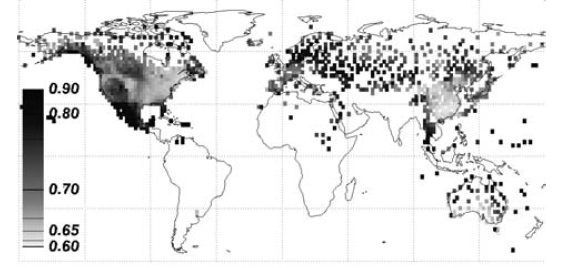
\includegraphics[width=0.8\columnwidth]{../figures/climate.jpg}\\
        
\includegraphics[width=\columnwidth]{../figures/networks-2.jpg}
      \end{column}
      \begin{column}{0.5\textwidth}
        
\includegraphics[width=\columnwidth]{../figures/dark_matter.jpg}
        \\
        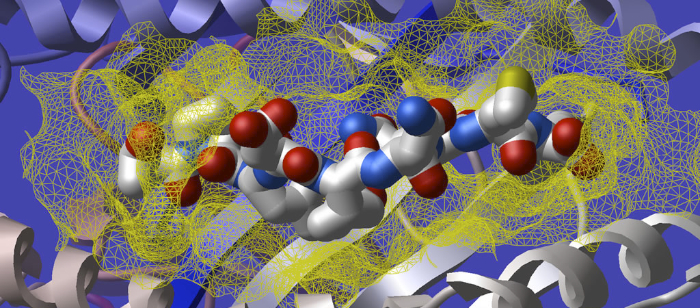
\includegraphics[width=\columnwidth]{../figures/protein.jpg}
      \end{column}
    \end{columns}
    \only<2>{
      \begin{tikzpicture}[remember picture,overlay]
        \draw[fill=black,opacity=0.75] 
        (current page.north east) rectangle (current page.south west);
        \node at (current page.center) {
          {\Huge \alert{Interpretability, Reproducibility}}
        };
      \end{tikzpicture}}
  \end{frame}
}

\only<article>{
  For that reason, science is a very natural application area for
  machine learning.  We can model the effects of climate change and
  how to mitigate it; discover structure in social networks; map
  the existence of dark matter in the universe by intelligently
  shifting through weak gravitational lens data, and not only study
  the mechanisms of protein folding, but discover methods to
  synthesize new drugs.

  We must be careful, however. In many cases we need to be able to
  interpret what our model tells us. We also must make sure that
  the any results we obtain are reproducible. This is something
  that we shall emphasize in this course.
}

\only<presentation>{
  \begin{frame}
    \frametitle{Pervasive ``intelligent'' systems}
    \begin{columns}
      \begin{column}{0.3\textwidth}
        \centering
        
\includegraphics[width=\textwidth]{../figures/echo-home.jpg}
        \\
        Home assistants

        \vspace{\fill}

        \bigskip

        
\includegraphics[width=\textwidth]{../figures/tesla.jpg}
        \\
        Autonomous vehicles
      \end{column}
      \begin{column}{0.3\textwidth}
        \centering 
        
\includegraphics[width=\textwidth]{../figures/web-ads.png}
        \\
        Web advertising

        \vspace{\fill}

        \bigskip

        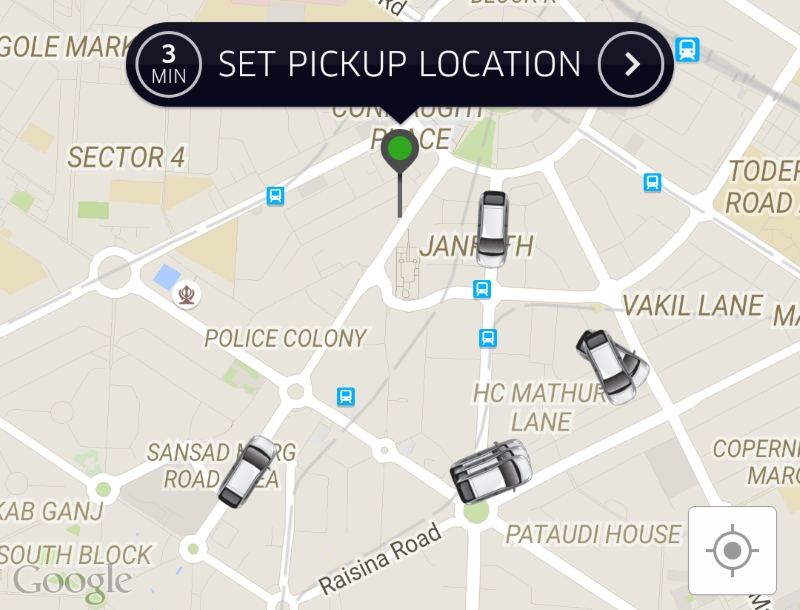
\includegraphics[width=\textwidth]{../figures/uber-here-maps.jpg}
        \\
        Ridesharing
      \end{column}
      \begin{column}{0.3\textwidth}
        \centering 
        \\
        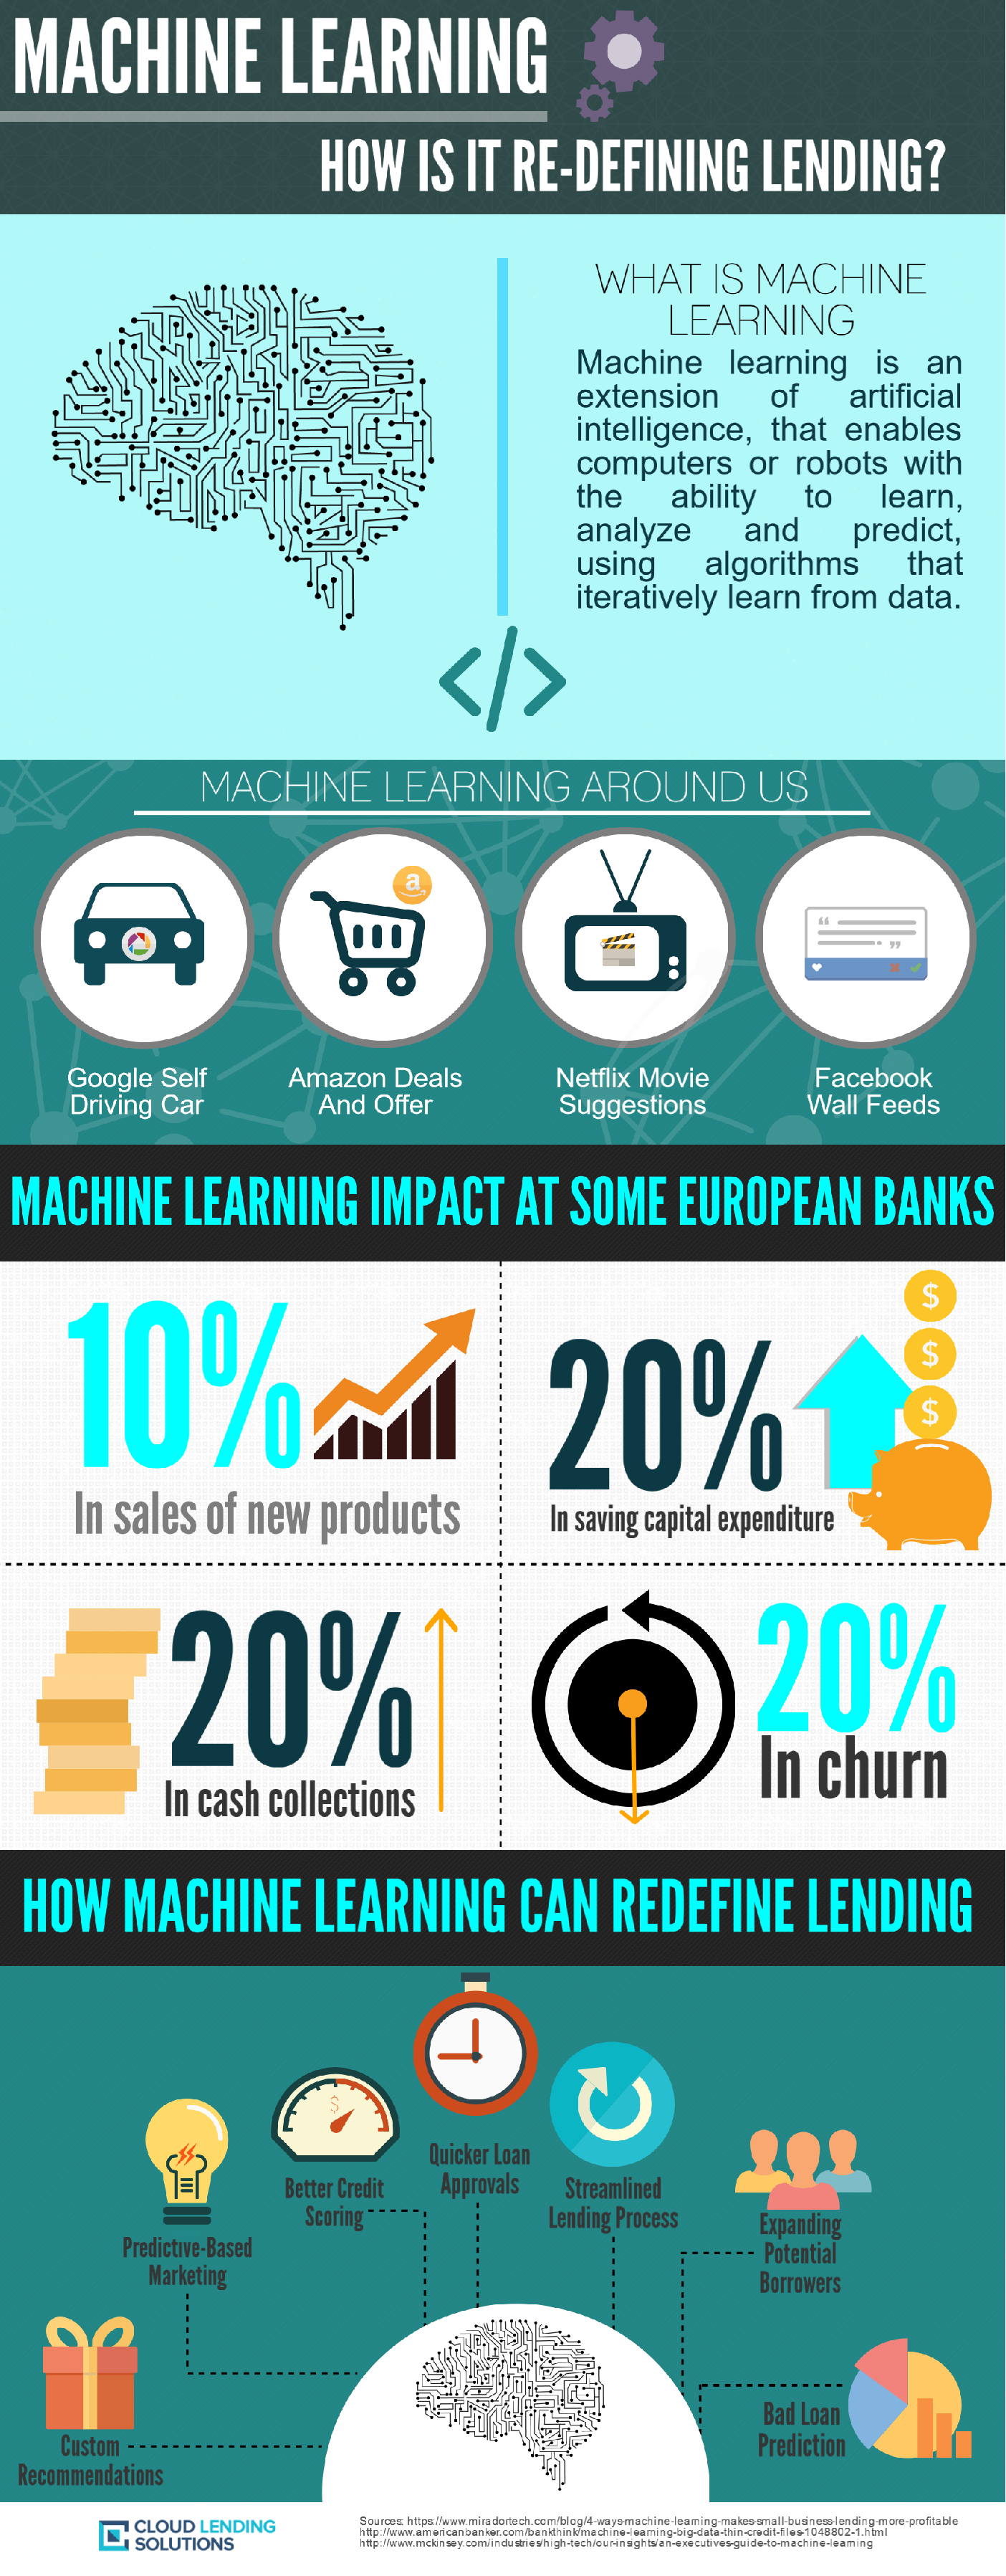
\includegraphics[width=\textwidth,clip = true, trim=0 0 0 42.5cm]{../figures/lending.pdf}
        \\
        Lending

        \vspace{\fill}

        \bigskip

        
\includegraphics[width=\textwidth]{../figures/algorithms-public.jpg}
        \\
        Public policy
      \end{column}
    \end{columns}
    \only<2>{
      \begin{tikzpicture}[remember picture,overlay]
        \draw[fill=black,opacity=0.75] 
        (current page.north east) rectangle (current page.south west);
        \node at (current page.center) {
          {\Huge \alert{Privacy, Fairness, Safety}}
        };
      \end{tikzpicture}}
  \end{frame}
}

\only<article>{
  While machine learning models in science are typically carefully
  handcrafted by scientists and experts in machine learning and
  statistics, this is not typically the case in everyday
  applications. Nevertheless, well-known or home-grown machine
  learning models are being deployed across the application
  spectrum. This involve home assistants that try and get you want,
  web advertising, which tries to find new things for you to want,
  lending, which tries to optimally lend you money so that you buy
  what you didn't need before. We also have autonomous vehicles,
  which take you were you want to go, and ridesharing services,
  which do the same thing, but use humans instead. Finally, there
  are many applications in public policy, such as crime prevention,
  justice, and disease control which use machine learning.  In all
  those cases, we have to worry about a great many things that are
  outside the scope of the machine learning problems itself. These
  are (a) privacy: you don't want your data used in ways that you have
  not consented to (b) fairness: you don't want minorities to be
  disadvantaged and (c) safety: you don't want your car to crash.
}

\subsection{Data analysis,  learning and planning}

\only<article>{
  To make the above more concrete, let's have a look at a number of problems in machine learning. These involve learning from and analysing data, including inferring decision rules, and constructing complex plans using the evidence gleaned from the data. Machine learning problems are commonly separated in three different types: supervised, unsupervised and reinforcement learning. Typical supervised learning problems include classification and regression, while unsupervised problems include compression, clustering and topic modelling. Reinforcement learning, on the other hand, is concerned with artificially intelligent agents more generally, with examples including game playing and adaptive control. Their main differences are two. Firstly, the \emph{type} of feedback we have about learning performance. Secondly, and perhaps more importantly, whether or not the problem involves \emph{active data collection}. In this course, we will try and take a global view of these problems in the context of decision theory.
}

\only<presentation>{
  \begin{frame}
    \centering
    \Huge{What can machine learning do?}
  \end{frame}
}
\begin{frame}
  \frametitle{Can machines learn from data?}
  \begin{center}
    \only<1>{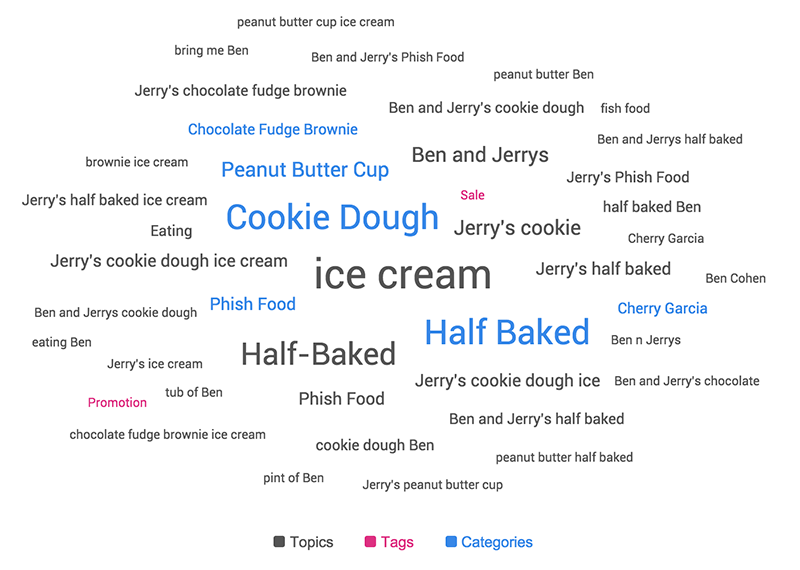
\includegraphics[width=0.8\textwidth]{../figures/text-cloud}
      \\

      {\large An unsupervised learning problem: topic modelling}
    }
    \only<2>{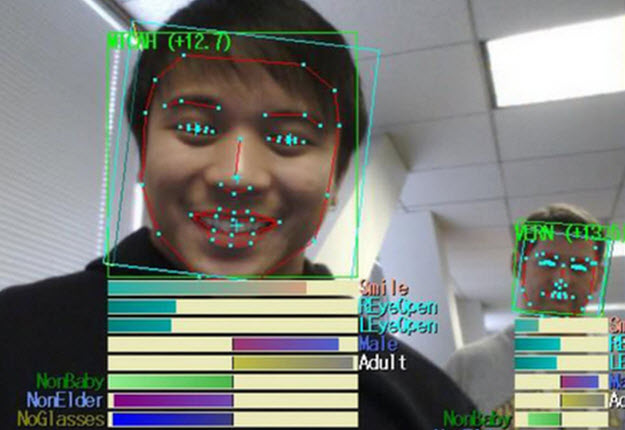
\includegraphics[width=0.8\textwidth]{../figures/Face-Recognition}
      \\

      {\large A supervised learning problem: object recognition}
    }
  \end{center}
\end{frame}


\only<article>{
  You can use machine learning just to analyse, or find structure in
  the data. This is generally called unsupervised learning. One such
  example is topic modelling, where you let the algorithm find topics
  from a corpus of text.  These days machines are used to learn from
  in many applications.  These include speech recognition, facial
  authentication, weather prediction, etc. In general, in these
  problems we are given a \emph{labelled} dataset with, say, example
  images from each class. Unfortunately this does not scale very
  well, because obtaining labels is expensive.

  This is partially how science works, because what we need to do
  is to find a general rule of nature from data. Starting from some
  hypothesis and some data, we reach a conclusion. However, many
  times we may need to actively experiment to obtain more data,
  perhaps because we found that our model is wrong.
}



\begin{frame}
  \frametitle{Can machines learn from their mistakes?}
  \begin{center}
    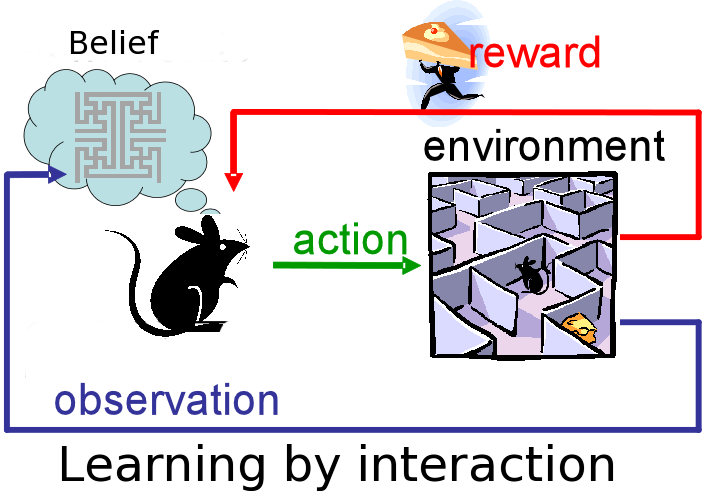
\includegraphics[width=0.7\textwidth]{../figures/rl_interaction}
  \end{center}
  \begin{block}{Reinforcement learning}
    Take actions $a_1, \ldots, a_t$, so as to maximise utility
    $U = \sum_{t=1}^T r_t$
  \end{block}
\end{frame}


\only<article>{
  So, what happens when we make a mistake? Can we somehow recognise
  it? Humans and other animals can actually learn from their
  mistakes. Consider the proverbial rat in the maze. At some
  intervals, the experimenter places some cheese in there, and the
  rat must do a series of actions to obtain it, such as navigating
  the maze and pulling some levers. It doesn't know how to get to
  the cheese easily, but it slowly learns the layout of the maze
  through observation, and in the end, through trial-and-error it
  is able to get to the cheese very efficiently.

  We can formalise this as a reinforcement learning problem, where
  the rat takes a series of actions; at each step it also obtains a
  reward, let's say equal to 0 when it has no cheese, and 1 when it
  eats cheese. Then we can declare that the rat's utility is the sum
  of all rewards over time, i.e. the total amount of cheese it can
  eat before it dies. The rat needs to explore the environment in order to be able to
  get to the cheese. 

  An example in robotics is trying to teach a
  robot to flip pancakes. One easy thing we can try is to show the robot
  how to do it, and then let it just copy the demonstrated
  movement. However, this doesn't work! The robot needs to explore
  variations of the movement, until it manages to successfully flip
  pancakes. Again, we can formulate this as a reinforcement learning
  problem, with a reward that is high whenever the pancake's position is
  flipped, and on the pan; and low everywhere else. Then the robot can
  learn to perform this behaviour through trial and error. It's
  important to note that in this example, merely demonstration is not
  enough. Neither is reinforcement learning enough. The same thing is
  true for the recent success of AlphaGo in beating a master human:
  apart from planning, they used both demonstration data and self-play,
  so that it could learn through trial and error.  }

\begin{frame}
  \frametitle{Can machines make complex plans?}
  \begin{center}
    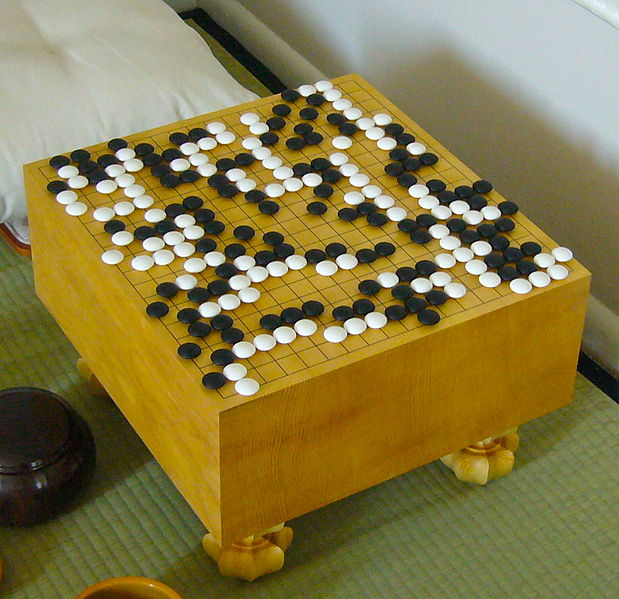
\includegraphics[width=0.8\textwidth]{../figures/619px-FloorGoban}
  \end{center}
\end{frame}


\only<article>{
  I suppose the first question is whether machines can plan
  ahead. Indeed, even for large problems, such as Go, machines can
  now perform at least as well as top-rated humans. How is this
  achieved?
}

\begin{frame}
  \frametitle{Machines can make complex plans!}
  \begin{center}
    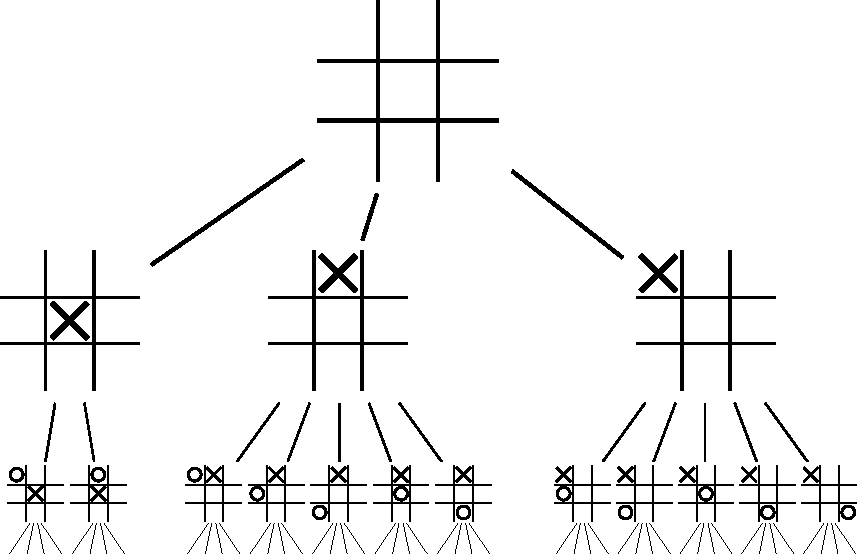
\includegraphics[width=0.8\textwidth]{../figures/Tic-tac-toe-game-tree}
  \end{center}
\end{frame}


\only<article>{
  The basic construction is the planning tree. This is an enumeration
  of all possible future events. If a complete enumeration is
  impossible, a partial tree is constructed. However this requires
  evaluating non-terminal game positions. In the old times, this was
  done with heuristics, but now this is data-driven, both through the
  use of expert databases, and through self-play and reinforcement
  learning.
}


\subsection{Experiment design}

\only<presentation>{
  \begin{frame}
    \centering
    \Huge{The scientific process as machine learning}
  \end{frame}
  \begin{frame}
    \centering
    
\includegraphics[width=\textwidth]{../figures/Las_Vegas_slot_machines}
  \end{frame}
}


\only<article>{
  An example that typifies trial and error learning are bandit
  problems. Imagine that you are in a Casino and you wish to
  maximise the amount of money you make during the night. There are
  a lot of machines to play. If you knew which one was the best,
  then you'd just play it all night long. However, you must also
  spend time trying out different machines, in order to get an
  estimate of how much money each one gives out. The trade off
  between trying out different machines and playing the one you
  currently think is best is called the exploration-exploitation
  trade-off and it appears in many problems of experiment design for
  science.
}


\begin{frame}
  \frametitle{Adam, the robot scientist}
  \centering
  
\includegraphics[width=0.8\textwidth]{../figures/robot-scientist}
\end{frame}


\only<article>{
  Let's say we want to build a robot scientist and tell it to
  discover a cure for cancer. What does the scientist do and how can the robot replicate it??
}



\begin{frame}
  \frametitle{Drug discovery}
  \centering
  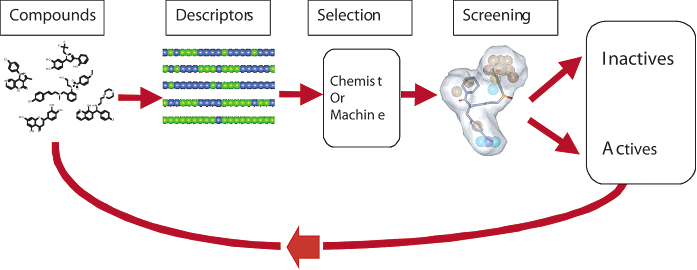
\includegraphics[width=\columnwidth]{../figures/drug-discovery-000}
\end{frame}


\only<article>{
  Simplifying the problem a bit, consider that you have a large
  number of drug candidates for cancer and you wish to discover
  those that are active against it. The ideas is that you select
  some of them, then screen them, to sort them into active and
  inactive. However, there are too many drugs to screen, so the
  process is interactive. At each cycle, we select some drugs to
  screen, classify them, and then use this information to select
  more drugs to screen. This cycle, consequently has two parts:
  1. Selecting some drugs given our current knowledge.
  2. Updating our knowledge given new evidence.
}


\begin{frame}
  \frametitle{Drawing conclusions from results}
  \centering
  \begin{tikzpicture}[line width=2pt]
    \node at (0,0) (bt) {hypothesis};
    \node[select] at (0,2) (at) {experiment};
    \node[utility] at (3,-2) (rt) {result};
    \draw[blue,->] (at) -- (rt);
    \node at (4,0) (bt2) {conclusion};
    \draw[red,->] (at) -- (bt2);
    \draw[red,->] (bt) -- (bt2);
    \draw[red,->] (rt) -- (bt2);
  \end{tikzpicture}
\end{frame}

\only<article>{
  In general, we would like to have some method which can draw
  conclusions from results. This involves starting with a
  hypothesis, performing an experiment to verify or refute it,
  obtain some experimental result; and then concluding for or
  against the hypothesis. Here the arrows show dependencies
  between these variables. So what do we mean by "hypothesis" in this case?
}

\subsection{Bayesian inference.}
\begin{frame}
  \frametitle{Tycho Brahe's minute eye measurements}
  \begin{columns}
    \begin{column}{0.5\textwidth}
      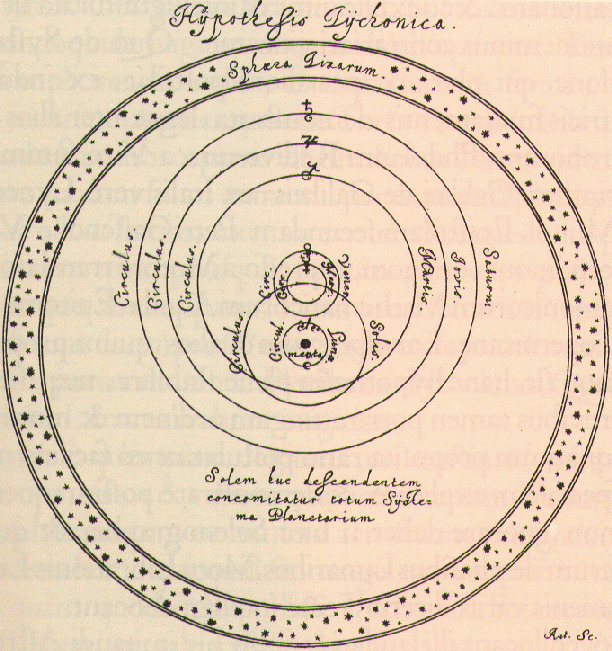
\includegraphics[width=0.5\textwidth]{../figures/circular-orbits}
    \end{column}
    \begin{column}{0.5\textwidth}
      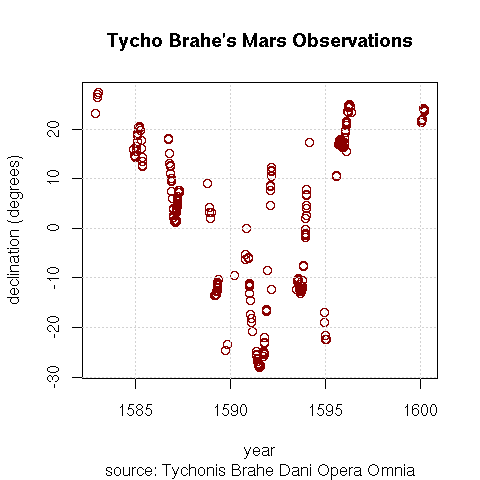
\includegraphics[width=0.5\textwidth]{../figures/tycho-observations}
    \end{column}
  \end{columns}
  \begin{itemize}
  \item Hypothesis: Circular orbits
  \item Conclusion: \alert{Specific} circular orbits
  \end{itemize}
\end{frame}


\only<article>{
  Let's take the example of planetary orbits. Here Tycho famously
  spent 20 years experimentally measuring the location of Mars. He
  had a hypothesis: that planetary orbits were circular, but he
  didn't know which were the right orbits. When he tried to fit his data to this hypothesis, he concluded a specific circular orbit for Mars \ldots around Earth.
}


\begin{frame}
  \frametitle{Johannes Kepler's alternative hypothesis}
  \begin{columns}
    \begin{column}{0.5\textwidth}
      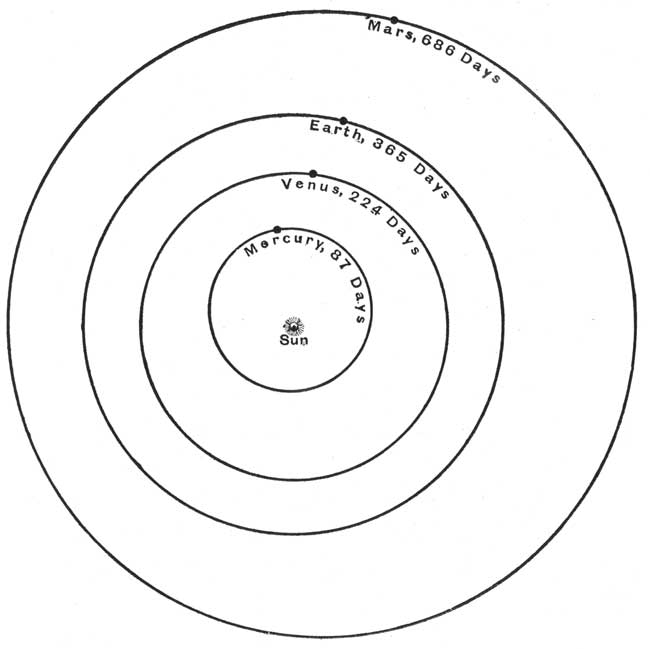
\includegraphics[width=0.5\textwidth]{../figures/orbits}
    \end{column}
    \begin{column}{0.5\textwidth}
      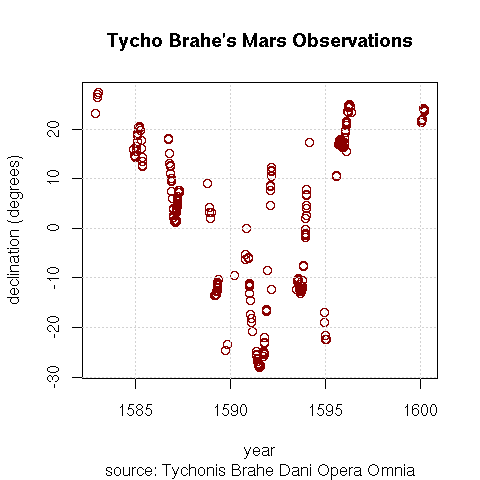
\includegraphics[width=0.5\textwidth]{../figures/tycho-observations}
    \end{column}
  \end{columns}
  \begin{itemize}
  \item Hypothesis: Circular \alert{or} elliptic orbits
  \item Conclusion: Specific \alert{elliptic} orbits
  \end{itemize}
\end{frame}


\only<article>{
  Kepler had a more general hypothesis: that orbits could be
  circular or elliptic, and he actually accepted that the planets
  orbited the sun. This led him to the broadly correct model of all
  planets being in elliptical orbits around the sun. However, the
  actual verification that all things do not revolve around earth,
  requires different experiments.
}


\begin{frame}
  \frametitle{200 years later, Gauss formalised this statistically}
  \begin{columns}
    \begin{column}{0.5\textwidth}
      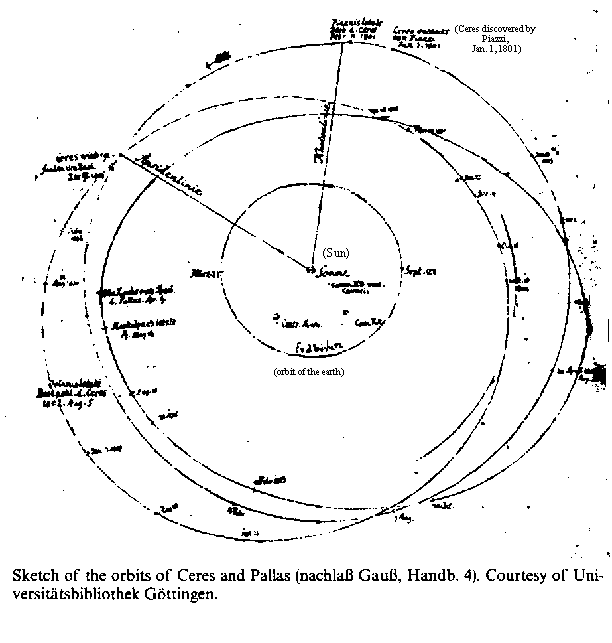
\includegraphics[width=\columnwidth]{../figures/gauss-diagram}
    \end{column}
    \begin{column}{0.5\textwidth}
      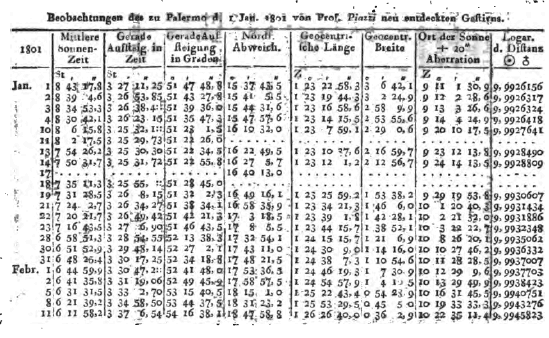
\includegraphics[width=\columnwidth]{../figures/SeptemberTable}
    \end{column}
  \end{columns}
\end{frame}


\only<article>{
  Later on, Gauss collected even more experimental data to calculate the orbit of Ceres. He did this using one of the first formal statistical methods; this allowed him to avoid cheating (like Kepler did, to accentuate his finding that orbits were elliptical).
}


\begin{frame}
  \frametitle{A warning: The dead salmon mirage}
  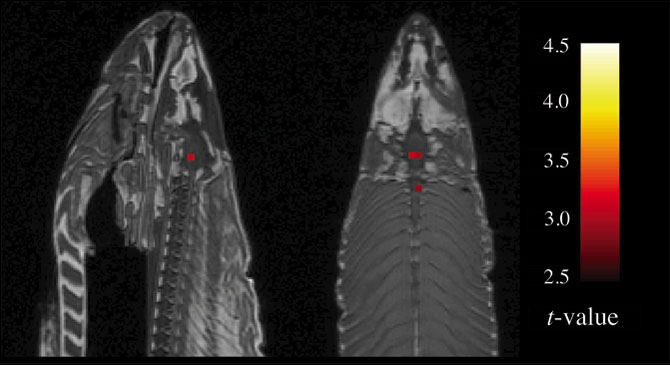
\includegraphics[width=\textwidth]{../figures/fmri-salmon}
\end{frame}


\only<article>{
  It is quite easy to draw the wrong conclusions from applying
  machine learning / statistics to your data. For example, it was
  fashionable to perform fMRI studies in humans to see whether some
  neurons have a particular functional role. There were even
  articles saying that "we found the neurons encoding for Angelina
  Jolie". So some scientists tried to replicate those results. They
  took a dead salmon, and put it an fMRI scanner. They checked its
  brain activity when it was shown images of happy or sad
  people. Perhaps surprisingly, they found an area of the brain that
  was correlated with the pictures - so it seemed, as though the
  dead salmon could distinguish photos of happy people from sad
  ones. However, this was all due to a misapplication of
  statistics. In this course, we will try and teach you to avoid
  such mistakes.
}


\begin{frame}
  \frametitle{Planning future experiments}
  \centering
  \begin{tikzpicture}[line width=2pt]
    \node at (0,0) (bt) {hypothesis};
    \node[select] at (0,2) (at) {experiment};
    \node[utility] at (3,-2) (rt) {result};
    \draw[blue,->] (at) -- (rt);
    \node at (4,0) (bt2) {conclusion};
    \draw[red,->] (at) -- (bt2);
    \draw[red,->] (bt) -- (bt2);
    \draw[red,->] (rt) -- (bt2);
  \end{tikzpicture}
\end{frame}

\only<article>{
  I mentioned before that we must decide what experiment to do. This is indeed difficult, especially in setting such as drug discovery where the number of experiments is huge.  However, conceptually, there is a simple and elegant solution to this problem.
}


\begin{frame}
  \frametitle{Planning experiments is like Tic-Tac-Toe}
  \begin{center}
    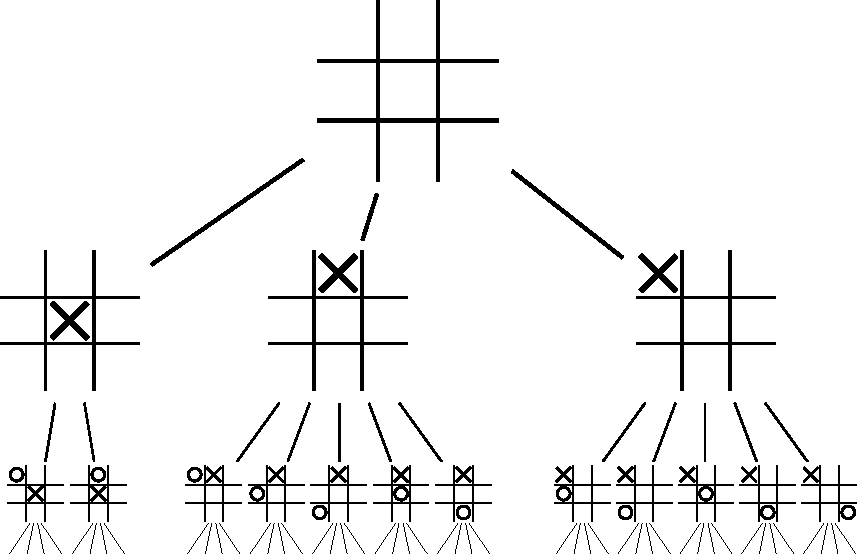
\includegraphics[width=\textwidth]{../figures/Tic-tac-toe-game-tree}
  \end{center}
\end{frame}


\only<article>{
  The basic idea is to think of experiment design as a game between the scientist and Nature. At every step, the scientist plays an X to  denote an experiment. Then Nature responds with an Observation. The main difference from a game is that Nature is (probably) not adversarial. We can also generalise this idea to problems in robotics, etc.
}

\only<presentation>{
  \begin{frame}
    \frametitle{Eve, another robot scientist}
    \centering \movie{
\includegraphics[width=\textwidth]{../figures/eve.jpg}}{Eve-video.mp4}
    Discovered a malaria drug
  \end{frame}
}
\only<article>{
  These kinds of techniques, coming from the reinforcement learning literature have been successfully used at the university of Manchester to create a robot, called Eve, that recently (re)-discovered a malaria drug.
}

\subsection{Course overview}

\begin{frame}
  \frametitle{Machine learning in practice}
  \begin{block}{Avoiding pitfalls}
    \begin{itemize}
    \item Choosing hypotheses.
    \item Correctly interpreting conclusions.
    \item Using a good testing methodology.
    \end{itemize}
  \end{block}
  \begin{block}{Machine learning in society}
    \begin{itemize}
    \item<alert@2> Privacy \uncover<2->{--- Medical data.}
    \item<alert@3> Fairness \uncover<3->{--- Credit risk.}
    \item<alert@4> Safety \uncover<4->{--- Autonomous vehicles.}
    \end{itemize}
  \end{block}
\end{frame}

\only<article>{
  One of the things we want to do in this course is teach you to
  avoid common pitfalls.

  Now I want to get into a different track. So far everything has
  been about pure research, but now machine learning is pervasive:
  Our phones, cars, watches, bathrooms, kettles are connected to the
  internet and send a continuous stream of data to companies. In
  addition, many companies and government actors use machine
  learning algorithms to make or support decisions. This creates a
  number of problems in privacy, fairness and safety.
}


\begin{frame}
  \frametitle{Technical topics}
  
  \begin{block}{Machine learning problems}
    \begin{itemize}
    \item Unsupervised learning.
    \item Supervised learning.
    \item Reinforcement learning.
    \end{itemize}
  \end{block}

  \begin{block}{Machine learning tools}
    \begin{itemize}
    \item Stochastic optimisation and neural networks.
    \item Probabilistic inference and Bayesian networks.
    \item Markov decision processes.
    \end{itemize}
  \end{block}
\end{frame}

\begin{frame}
  \frametitle{Course structure}
  \begin{block}{Module structure}
    \begin{itemize}
    \item \alert{Activity}-based, hands-on.
    \item Background reading \alert{before} class.
    \item Mini-lecture with \alert{Q/A} at each class.
    \item Small \alert{group project} in second half of class.
    \end{itemize}
  \end{block}

  \begin{block}{Modules}
    \begin{itemize}
    \item Medical diagnostics.
    \item Speech recognition.
    \item Recommendation systems.
    \item Helicopter flight.
    \end{itemize}
  \end{block}
\end{frame}


\section{Nearest neighbours}
\begin{frame}
  \frametitle{Discriminating between diseases}
  % Title: glps_renderer figure
% Creator: GL2PS 1.3.8, (C) 1999-2012 C. Geuzaine
% For: Octave
% CreationDate: Fri Jun 16 12:38:10 2017
\begin{pgfpicture}
\pgfsetlinewidth{0.01pt}
\color[rgb]{1.000000,1.000000,1.000000}
\pgfpathmoveto{\pgfpoint{41.600006pt}{205.577454pt}}
\pgflineto{\pgfpoint{289.600037pt}{140.777435pt}}
\pgflineto{\pgfpoint{41.600006pt}{140.777435pt}}
\pgfpathclose
\pgfusepath{fill,stroke}
\pgfpathmoveto{\pgfpoint{41.600006pt}{205.577454pt}}
\pgflineto{\pgfpoint{289.600037pt}{205.577454pt}}
\pgflineto{\pgfpoint{289.600037pt}{140.777435pt}}
\pgfpathclose
\pgfusepath{fill,stroke}
\pgfpathmoveto{\pgfpoint{41.600006pt}{91.199989pt}}
\pgflineto{\pgfpoint{289.600037pt}{26.399979pt}}
\pgflineto{\pgfpoint{41.600006pt}{26.399979pt}}
\pgfpathclose
\pgfusepath{fill,stroke}
\pgfpathmoveto{\pgfpoint{41.600006pt}{91.199989pt}}
\pgflineto{\pgfpoint{289.600037pt}{91.199989pt}}
\pgflineto{\pgfpoint{289.600037pt}{26.399979pt}}
\pgfpathclose
\pgfusepath{fill,stroke}
\color[rgb]{1.000000,0.000000,0.000000}
\pgfpathmoveto{\pgfpoint{287.608032pt}{140.777435pt}}
\pgflineto{\pgfpoint{288.604004pt}{140.777435pt}}
\pgflineto{\pgfpoint{288.604004pt}{142.317886pt}}
\pgfpathclose
\pgfusepath{fill,stroke}
\pgfpathmoveto{\pgfpoint{289.600037pt}{141.234161pt}}
\pgflineto{\pgfpoint{288.604004pt}{142.317886pt}}
\pgflineto{\pgfpoint{288.604004pt}{140.777435pt}}
\pgfpathclose
\pgfusepath{fill,stroke}
\pgfpathmoveto{\pgfpoint{289.600037pt}{140.777435pt}}
\pgflineto{\pgfpoint{289.600037pt}{141.234161pt}}
\pgflineto{\pgfpoint{288.604004pt}{140.777435pt}}
\pgfpathclose
\pgfusepath{fill,stroke}
\pgfpathmoveto{\pgfpoint{283.624115pt}{140.777435pt}}
\pgflineto{\pgfpoint{284.620087pt}{140.777435pt}}
\pgflineto{\pgfpoint{284.620087pt}{140.819778pt}}
\pgfpathclose
\pgfusepath{fill,stroke}
\pgfpathmoveto{\pgfpoint{285.616089pt}{141.090790pt}}
\pgflineto{\pgfpoint{284.620087pt}{140.819778pt}}
\pgflineto{\pgfpoint{284.620087pt}{140.777435pt}}
\pgfpathclose
\pgfusepath{fill,stroke}
\pgfpathmoveto{\pgfpoint{285.616089pt}{140.777435pt}}
\pgflineto{\pgfpoint{285.616089pt}{141.090790pt}}
\pgflineto{\pgfpoint{284.620087pt}{140.777435pt}}
\pgfpathclose
\pgfusepath{fill,stroke}
\pgfpathmoveto{\pgfpoint{286.612061pt}{140.777435pt}}
\pgflineto{\pgfpoint{285.616089pt}{141.090790pt}}
\pgflineto{\pgfpoint{285.616089pt}{140.777435pt}}
\pgfpathclose
\pgfusepath{fill,stroke}
\pgfpathmoveto{\pgfpoint{275.656250pt}{140.777435pt}}
\pgflineto{\pgfpoint{276.652222pt}{140.777435pt}}
\pgflineto{\pgfpoint{276.652222pt}{141.883286pt}}
\pgfpathclose
\pgfusepath{fill,stroke}
\pgfpathmoveto{\pgfpoint{277.648193pt}{145.700470pt}}
\pgflineto{\pgfpoint{276.652222pt}{141.883286pt}}
\pgflineto{\pgfpoint{276.652222pt}{140.777435pt}}
\pgfpathclose
\pgfusepath{fill,stroke}
\pgfpathmoveto{\pgfpoint{277.648193pt}{140.777435pt}}
\pgflineto{\pgfpoint{277.648193pt}{145.700470pt}}
\pgflineto{\pgfpoint{276.652222pt}{140.777435pt}}
\pgfpathclose
\pgfusepath{fill,stroke}
\pgfpathmoveto{\pgfpoint{278.644196pt}{141.350510pt}}
\pgflineto{\pgfpoint{277.648193pt}{145.700470pt}}
\pgflineto{\pgfpoint{277.648193pt}{140.777435pt}}
\pgfpathclose
\pgfusepath{fill,stroke}
\pgfpathmoveto{\pgfpoint{278.644196pt}{140.777435pt}}
\pgflineto{\pgfpoint{278.644196pt}{141.350510pt}}
\pgflineto{\pgfpoint{277.648193pt}{140.777435pt}}
\pgfpathclose
\pgfusepath{fill,stroke}
\pgfpathmoveto{\pgfpoint{279.640167pt}{141.685425pt}}
\pgflineto{\pgfpoint{278.644196pt}{141.350510pt}}
\pgflineto{\pgfpoint{278.644196pt}{140.777435pt}}
\pgfpathclose
\pgfusepath{fill,stroke}
\pgfpathmoveto{\pgfpoint{279.640167pt}{140.777435pt}}
\pgflineto{\pgfpoint{279.640167pt}{141.685425pt}}
\pgflineto{\pgfpoint{278.644196pt}{140.777435pt}}
\pgfpathclose
\pgfusepath{fill,stroke}
\pgfpathmoveto{\pgfpoint{280.636139pt}{140.839111pt}}
\pgflineto{\pgfpoint{279.640167pt}{141.685425pt}}
\pgflineto{\pgfpoint{279.640167pt}{140.777435pt}}
\pgfpathclose
\pgfusepath{fill,stroke}
\pgfpathmoveto{\pgfpoint{280.636139pt}{140.777435pt}}
\pgflineto{\pgfpoint{280.636139pt}{140.839111pt}}
\pgflineto{\pgfpoint{279.640167pt}{140.777435pt}}
\pgfpathclose
\pgfusepath{fill,stroke}
\pgfpathmoveto{\pgfpoint{281.632141pt}{140.783401pt}}
\pgflineto{\pgfpoint{280.636139pt}{140.839111pt}}
\pgflineto{\pgfpoint{280.636139pt}{140.777435pt}}
\pgfpathclose
\pgfusepath{fill,stroke}
\pgfpathmoveto{\pgfpoint{281.632141pt}{140.777435pt}}
\pgflineto{\pgfpoint{281.632141pt}{140.783401pt}}
\pgflineto{\pgfpoint{280.636139pt}{140.777435pt}}
\pgfpathclose
\pgfusepath{fill,stroke}
\pgfpathmoveto{\pgfpoint{282.628113pt}{141.247986pt}}
\pgflineto{\pgfpoint{281.632141pt}{140.783401pt}}
\pgflineto{\pgfpoint{281.632141pt}{140.777435pt}}
\pgfpathclose
\pgfusepath{fill,stroke}
\pgfpathmoveto{\pgfpoint{282.628113pt}{140.777435pt}}
\pgflineto{\pgfpoint{282.628113pt}{141.247986pt}}
\pgflineto{\pgfpoint{281.632141pt}{140.777435pt}}
\pgfpathclose
\pgfusepath{fill,stroke}
\pgfpathmoveto{\pgfpoint{283.624115pt}{140.777435pt}}
\pgflineto{\pgfpoint{282.628113pt}{141.247986pt}}
\pgflineto{\pgfpoint{282.628113pt}{140.777435pt}}
\pgfpathclose
\pgfusepath{fill,stroke}
\pgfpathmoveto{\pgfpoint{262.708435pt}{140.777435pt}}
\pgflineto{\pgfpoint{263.704407pt}{140.777435pt}}
\pgflineto{\pgfpoint{263.704407pt}{149.672318pt}}
\pgfpathclose
\pgfusepath{fill,stroke}
\pgfpathmoveto{\pgfpoint{264.700409pt}{150.470245pt}}
\pgflineto{\pgfpoint{263.704407pt}{149.672318pt}}
\pgflineto{\pgfpoint{263.704407pt}{140.777435pt}}
\pgfpathclose
\pgfusepath{fill,stroke}
\pgfpathmoveto{\pgfpoint{264.700409pt}{140.777435pt}}
\pgflineto{\pgfpoint{264.700409pt}{150.470245pt}}
\pgflineto{\pgfpoint{263.704407pt}{140.777435pt}}
\pgfpathclose
\pgfusepath{fill,stroke}
\pgfpathmoveto{\pgfpoint{265.696411pt}{146.772659pt}}
\pgflineto{\pgfpoint{264.700409pt}{150.470245pt}}
\pgflineto{\pgfpoint{264.700409pt}{140.777435pt}}
\pgfpathclose
\pgfusepath{fill,stroke}
\pgfpathmoveto{\pgfpoint{265.696411pt}{140.777435pt}}
\pgflineto{\pgfpoint{265.696411pt}{146.772659pt}}
\pgflineto{\pgfpoint{264.700409pt}{140.777435pt}}
\pgfpathclose
\pgfusepath{fill,stroke}
\pgfpathmoveto{\pgfpoint{266.692383pt}{141.012543pt}}
\pgflineto{\pgfpoint{265.696411pt}{146.772659pt}}
\pgflineto{\pgfpoint{265.696411pt}{140.777435pt}}
\pgfpathclose
\pgfusepath{fill,stroke}
\pgfpathmoveto{\pgfpoint{266.692383pt}{140.777435pt}}
\pgflineto{\pgfpoint{266.692383pt}{141.012543pt}}
\pgflineto{\pgfpoint{265.696411pt}{140.777435pt}}
\pgfpathclose
\pgfusepath{fill,stroke}
\pgfpathmoveto{\pgfpoint{267.688354pt}{140.947601pt}}
\pgflineto{\pgfpoint{266.692383pt}{141.012543pt}}
\pgflineto{\pgfpoint{266.692383pt}{140.777435pt}}
\pgfpathclose
\pgfusepath{fill,stroke}
\pgfpathmoveto{\pgfpoint{267.688354pt}{140.777435pt}}
\pgflineto{\pgfpoint{267.688354pt}{140.947601pt}}
\pgflineto{\pgfpoint{266.692383pt}{140.777435pt}}
\pgfpathclose
\pgfusepath{fill,stroke}
\pgfpathmoveto{\pgfpoint{268.684326pt}{165.780823pt}}
\pgflineto{\pgfpoint{267.688354pt}{140.947601pt}}
\pgflineto{\pgfpoint{267.688354pt}{140.777435pt}}
\pgfpathclose
\pgfusepath{fill,stroke}
\pgfpathmoveto{\pgfpoint{268.684326pt}{140.777435pt}}
\pgflineto{\pgfpoint{268.684326pt}{165.780823pt}}
\pgflineto{\pgfpoint{267.688354pt}{140.777435pt}}
\pgfpathclose
\pgfusepath{fill,stroke}
\pgfpathmoveto{\pgfpoint{269.680328pt}{142.178589pt}}
\pgflineto{\pgfpoint{268.684326pt}{165.780823pt}}
\pgflineto{\pgfpoint{268.684326pt}{140.777435pt}}
\pgfpathclose
\pgfusepath{fill,stroke}
\pgfpathmoveto{\pgfpoint{269.680328pt}{140.777435pt}}
\pgflineto{\pgfpoint{269.680328pt}{142.178589pt}}
\pgflineto{\pgfpoint{268.684326pt}{140.777435pt}}
\pgfpathclose
\pgfusepath{fill,stroke}
\pgfpathmoveto{\pgfpoint{270.676331pt}{140.852936pt}}
\pgflineto{\pgfpoint{269.680328pt}{142.178589pt}}
\pgflineto{\pgfpoint{269.680328pt}{140.777435pt}}
\pgfpathclose
\pgfusepath{fill,stroke}
\pgfpathmoveto{\pgfpoint{270.676331pt}{140.777435pt}}
\pgflineto{\pgfpoint{270.676331pt}{140.852936pt}}
\pgflineto{\pgfpoint{269.680328pt}{140.777435pt}}
\pgfpathclose
\pgfusepath{fill,stroke}
\pgfpathmoveto{\pgfpoint{271.672302pt}{149.853119pt}}
\pgflineto{\pgfpoint{270.676331pt}{140.852936pt}}
\pgflineto{\pgfpoint{270.676331pt}{140.777435pt}}
\pgfpathclose
\pgfusepath{fill,stroke}
\pgfpathmoveto{\pgfpoint{271.672302pt}{140.777435pt}}
\pgflineto{\pgfpoint{271.672302pt}{149.853119pt}}
\pgflineto{\pgfpoint{270.676331pt}{140.777435pt}}
\pgfpathclose
\pgfusepath{fill,stroke}
\pgfpathmoveto{\pgfpoint{272.668274pt}{167.198486pt}}
\pgflineto{\pgfpoint{271.672302pt}{149.853119pt}}
\pgflineto{\pgfpoint{271.672302pt}{140.777435pt}}
\pgfpathclose
\pgfusepath{fill,stroke}
\pgfpathmoveto{\pgfpoint{272.668274pt}{140.777435pt}}
\pgflineto{\pgfpoint{272.668274pt}{167.198486pt}}
\pgflineto{\pgfpoint{271.672302pt}{140.777435pt}}
\pgfpathclose
\pgfusepath{fill,stroke}
\pgfpathmoveto{\pgfpoint{273.664276pt}{140.777435pt}}
\pgflineto{\pgfpoint{272.668274pt}{167.198486pt}}
\pgflineto{\pgfpoint{272.668274pt}{140.777435pt}}
\pgfpathclose
\pgfusepath{fill,stroke}
\pgfpathmoveto{\pgfpoint{255.736542pt}{140.777435pt}}
\pgflineto{\pgfpoint{256.732544pt}{140.777435pt}}
\pgflineto{\pgfpoint{256.732544pt}{160.055664pt}}
\pgfpathclose
\pgfusepath{fill,stroke}
\pgfpathmoveto{\pgfpoint{257.728516pt}{145.276688pt}}
\pgflineto{\pgfpoint{256.732544pt}{160.055664pt}}
\pgflineto{\pgfpoint{256.732544pt}{140.777435pt}}
\pgfpathclose
\pgfusepath{fill,stroke}
\pgfpathmoveto{\pgfpoint{257.728516pt}{140.777435pt}}
\pgflineto{\pgfpoint{257.728516pt}{145.276688pt}}
\pgflineto{\pgfpoint{256.732544pt}{140.777435pt}}
\pgfpathclose
\pgfusepath{fill,stroke}
\pgfpathmoveto{\pgfpoint{258.724518pt}{145.143265pt}}
\pgflineto{\pgfpoint{257.728516pt}{145.276688pt}}
\pgflineto{\pgfpoint{257.728516pt}{140.777435pt}}
\pgfpathclose
\pgfusepath{fill,stroke}
\pgfpathmoveto{\pgfpoint{258.724518pt}{140.777435pt}}
\pgflineto{\pgfpoint{258.724518pt}{145.143265pt}}
\pgflineto{\pgfpoint{257.728516pt}{140.777435pt}}
\pgfpathclose
\pgfusepath{fill,stroke}
\pgfpathmoveto{\pgfpoint{259.720490pt}{141.107025pt}}
\pgflineto{\pgfpoint{258.724518pt}{145.143265pt}}
\pgflineto{\pgfpoint{258.724518pt}{140.777435pt}}
\pgfpathclose
\pgfusepath{fill,stroke}
\pgfpathmoveto{\pgfpoint{259.720490pt}{140.777435pt}}
\pgflineto{\pgfpoint{259.720490pt}{141.107025pt}}
\pgflineto{\pgfpoint{258.724518pt}{140.777435pt}}
\pgfpathclose
\pgfusepath{fill,stroke}
\pgfpathmoveto{\pgfpoint{260.716492pt}{140.785751pt}}
\pgflineto{\pgfpoint{259.720490pt}{141.107025pt}}
\pgflineto{\pgfpoint{259.720490pt}{140.777435pt}}
\pgfpathclose
\pgfusepath{fill,stroke}
\pgfpathmoveto{\pgfpoint{260.716492pt}{140.777435pt}}
\pgflineto{\pgfpoint{260.716492pt}{140.785751pt}}
\pgflineto{\pgfpoint{259.720490pt}{140.777435pt}}
\pgfpathclose
\pgfusepath{fill,stroke}
\pgfpathmoveto{\pgfpoint{261.712463pt}{140.881470pt}}
\pgflineto{\pgfpoint{260.716492pt}{140.785751pt}}
\pgflineto{\pgfpoint{260.716492pt}{140.777435pt}}
\pgfpathclose
\pgfusepath{fill,stroke}
\pgfpathmoveto{\pgfpoint{261.712463pt}{140.777435pt}}
\pgflineto{\pgfpoint{261.712463pt}{140.881470pt}}
\pgflineto{\pgfpoint{260.716492pt}{140.777435pt}}
\pgfpathclose
\pgfusepath{fill,stroke}
\pgfpathmoveto{\pgfpoint{262.708435pt}{140.777435pt}}
\pgflineto{\pgfpoint{261.712463pt}{140.881470pt}}
\pgflineto{\pgfpoint{261.712463pt}{140.777435pt}}
\pgfpathclose
\pgfusepath{fill,stroke}
\pgfpathmoveto{\pgfpoint{252.748611pt}{140.777435pt}}
\pgflineto{\pgfpoint{253.744598pt}{205.642242pt}}
\pgflineto{\pgfpoint{253.234100pt}{205.642242pt}}
\pgfpathclose
\pgfusepath{fill,stroke}
\pgfpathmoveto{\pgfpoint{252.748611pt}{140.777435pt}}
\pgflineto{\pgfpoint{253.744598pt}{140.777435pt}}
\pgflineto{\pgfpoint{253.744598pt}{205.642242pt}}
\pgfpathclose
\pgfusepath{fill,stroke}
\pgfpathmoveto{\pgfpoint{254.325424pt}{205.642242pt}}
\pgflineto{\pgfpoint{253.744598pt}{205.642242pt}}
\pgflineto{\pgfpoint{253.744598pt}{140.777435pt}}
\pgfpathclose
\pgfusepath{fill,stroke}
\pgfpathmoveto{\pgfpoint{254.740570pt}{140.777435pt}}
\pgflineto{\pgfpoint{254.325424pt}{205.642242pt}}
\pgflineto{\pgfpoint{253.744598pt}{140.777435pt}}
\pgfpathclose
\pgfusepath{fill,stroke}
\pgfpathmoveto{\pgfpoint{254.740570pt}{140.777435pt}}
\pgflineto{\pgfpoint{254.740570pt}{205.642242pt}}
\pgflineto{\pgfpoint{254.325424pt}{205.642242pt}}
\pgfpathclose
\pgfusepath{fill,stroke}
\pgfpathmoveto{\pgfpoint{255.736542pt}{140.777435pt}}
\pgflineto{\pgfpoint{254.740570pt}{205.642242pt}}
\pgflineto{\pgfpoint{254.740570pt}{140.777435pt}}
\pgfpathclose
\pgfusepath{fill,stroke}
\pgfpathmoveto{\pgfpoint{255.736542pt}{140.777435pt}}
\pgflineto{\pgfpoint{255.155716pt}{205.642242pt}}
\pgflineto{\pgfpoint{254.740570pt}{205.642242pt}}
\pgfpathclose
\pgfusepath{fill,stroke}
\pgfpathmoveto{\pgfpoint{244.780731pt}{140.777435pt}}
\pgflineto{\pgfpoint{245.776718pt}{140.777435pt}}
\pgflineto{\pgfpoint{245.776718pt}{140.921082pt}}
\pgfpathclose
\pgfusepath{fill,stroke}
\pgfpathmoveto{\pgfpoint{246.231064pt}{205.642242pt}}
\pgflineto{\pgfpoint{245.776718pt}{140.921082pt}}
\pgflineto{\pgfpoint{245.776718pt}{140.777435pt}}
\pgfpathclose
\pgfusepath{fill,stroke}
\pgfpathmoveto{\pgfpoint{246.231064pt}{205.642242pt}}
\pgflineto{\pgfpoint{246.230515pt}{205.642242pt}}
\pgflineto{\pgfpoint{245.776718pt}{140.921082pt}}
\pgfpathclose
\pgfusepath{fill,stroke}
\pgfpathmoveto{\pgfpoint{246.772705pt}{140.777435pt}}
\pgflineto{\pgfpoint{246.231064pt}{205.642242pt}}
\pgflineto{\pgfpoint{245.776718pt}{140.777435pt}}
\pgfpathclose
\pgfusepath{fill,stroke}
\pgfpathmoveto{\pgfpoint{246.772705pt}{140.777435pt}}
\pgflineto{\pgfpoint{246.772705pt}{205.642242pt}}
\pgflineto{\pgfpoint{246.231064pt}{205.642242pt}}
\pgfpathclose
\pgfusepath{fill,stroke}
\pgfpathmoveto{\pgfpoint{247.768677pt}{144.035980pt}}
\pgflineto{\pgfpoint{246.772705pt}{205.642242pt}}
\pgflineto{\pgfpoint{246.772705pt}{140.777435pt}}
\pgfpathclose
\pgfusepath{fill,stroke}
\pgfpathmoveto{\pgfpoint{247.768677pt}{144.035980pt}}
\pgflineto{\pgfpoint{247.327042pt}{205.642242pt}}
\pgflineto{\pgfpoint{246.772705pt}{205.642242pt}}
\pgfpathclose
\pgfusepath{fill,stroke}
\pgfpathmoveto{\pgfpoint{247.768677pt}{140.777435pt}}
\pgflineto{\pgfpoint{247.768677pt}{144.035980pt}}
\pgflineto{\pgfpoint{246.772705pt}{140.777435pt}}
\pgfpathclose
\pgfusepath{fill,stroke}
\pgfpathmoveto{\pgfpoint{248.764679pt}{140.987183pt}}
\pgflineto{\pgfpoint{247.768677pt}{144.035980pt}}
\pgflineto{\pgfpoint{247.768677pt}{140.777435pt}}
\pgfpathclose
\pgfusepath{fill,stroke}
\pgfpathmoveto{\pgfpoint{248.764679pt}{140.777435pt}}
\pgflineto{\pgfpoint{248.764679pt}{140.987183pt}}
\pgflineto{\pgfpoint{247.768677pt}{140.777435pt}}
\pgfpathclose
\pgfusepath{fill,stroke}
\pgfpathmoveto{\pgfpoint{249.760651pt}{140.861908pt}}
\pgflineto{\pgfpoint{248.764679pt}{140.987183pt}}
\pgflineto{\pgfpoint{248.764679pt}{140.777435pt}}
\pgfpathclose
\pgfusepath{fill,stroke}
\pgfpathmoveto{\pgfpoint{249.760651pt}{140.777435pt}}
\pgflineto{\pgfpoint{249.760651pt}{140.861908pt}}
\pgflineto{\pgfpoint{248.764679pt}{140.777435pt}}
\pgfpathclose
\pgfusepath{fill,stroke}
\pgfpathmoveto{\pgfpoint{250.756638pt}{143.997910pt}}
\pgflineto{\pgfpoint{249.760651pt}{140.861908pt}}
\pgflineto{\pgfpoint{249.760651pt}{140.777435pt}}
\pgfpathclose
\pgfusepath{fill,stroke}
\pgfpathmoveto{\pgfpoint{250.756638pt}{140.777435pt}}
\pgflineto{\pgfpoint{250.756638pt}{143.997910pt}}
\pgflineto{\pgfpoint{249.760651pt}{140.777435pt}}
\pgfpathclose
\pgfusepath{fill,stroke}
\pgfpathmoveto{\pgfpoint{251.752625pt}{140.777435pt}}
\pgflineto{\pgfpoint{250.756638pt}{143.997910pt}}
\pgflineto{\pgfpoint{250.756638pt}{140.777435pt}}
\pgfpathclose
\pgfusepath{fill,stroke}
\pgfpathmoveto{\pgfpoint{241.792786pt}{140.777435pt}}
\pgflineto{\pgfpoint{242.788757pt}{140.777435pt}}
\pgflineto{\pgfpoint{242.788757pt}{141.050537pt}}
\pgfpathclose
\pgfusepath{fill,stroke}
\pgfpathmoveto{\pgfpoint{243.784744pt}{140.826157pt}}
\pgflineto{\pgfpoint{242.788757pt}{141.050537pt}}
\pgflineto{\pgfpoint{242.788757pt}{140.777435pt}}
\pgfpathclose
\pgfusepath{fill,stroke}
\pgfpathmoveto{\pgfpoint{243.784744pt}{140.777435pt}}
\pgflineto{\pgfpoint{243.784744pt}{140.826157pt}}
\pgflineto{\pgfpoint{242.788757pt}{140.777435pt}}
\pgfpathclose
\pgfusepath{fill,stroke}
\pgfpathmoveto{\pgfpoint{244.780731pt}{140.777435pt}}
\pgflineto{\pgfpoint{243.784744pt}{140.826157pt}}
\pgflineto{\pgfpoint{243.784744pt}{140.777435pt}}
\pgfpathclose
\pgfusepath{fill,stroke}
\pgfpathmoveto{\pgfpoint{239.800812pt}{140.777435pt}}
\pgflineto{\pgfpoint{240.796814pt}{140.777435pt}}
\pgflineto{\pgfpoint{240.796814pt}{141.635849pt}}
\pgfpathclose
\pgfusepath{fill,stroke}
\pgfpathmoveto{\pgfpoint{241.792786pt}{140.777435pt}}
\pgflineto{\pgfpoint{240.796814pt}{141.635849pt}}
\pgflineto{\pgfpoint{240.796814pt}{140.777435pt}}
\pgfpathclose
\pgfusepath{fill,stroke}
\pgfpathmoveto{\pgfpoint{232.828934pt}{140.777435pt}}
\pgflineto{\pgfpoint{233.824921pt}{140.777435pt}}
\pgflineto{\pgfpoint{233.824921pt}{143.663483pt}}
\pgfpathclose
\pgfusepath{fill,stroke}
\pgfpathmoveto{\pgfpoint{234.820892pt}{144.424850pt}}
\pgflineto{\pgfpoint{233.824921pt}{143.663483pt}}
\pgflineto{\pgfpoint{233.824921pt}{140.777435pt}}
\pgfpathclose
\pgfusepath{fill,stroke}
\pgfpathmoveto{\pgfpoint{234.820892pt}{140.777435pt}}
\pgflineto{\pgfpoint{234.820892pt}{144.424850pt}}
\pgflineto{\pgfpoint{233.824921pt}{140.777435pt}}
\pgfpathclose
\pgfusepath{fill,stroke}
\pgfpathmoveto{\pgfpoint{235.816864pt}{141.070068pt}}
\pgflineto{\pgfpoint{234.820892pt}{144.424850pt}}
\pgflineto{\pgfpoint{234.820892pt}{140.777435pt}}
\pgfpathclose
\pgfusepath{fill,stroke}
\pgfpathmoveto{\pgfpoint{235.816864pt}{140.777435pt}}
\pgflineto{\pgfpoint{235.816864pt}{141.070068pt}}
\pgflineto{\pgfpoint{234.820892pt}{140.777435pt}}
\pgfpathclose
\pgfusepath{fill,stroke}
\pgfpathmoveto{\pgfpoint{236.812866pt}{141.387177pt}}
\pgflineto{\pgfpoint{235.816864pt}{141.070068pt}}
\pgflineto{\pgfpoint{235.816864pt}{140.777435pt}}
\pgfpathclose
\pgfusepath{fill,stroke}
\pgfpathmoveto{\pgfpoint{236.812866pt}{140.777435pt}}
\pgflineto{\pgfpoint{236.812866pt}{141.387177pt}}
\pgflineto{\pgfpoint{235.816864pt}{140.777435pt}}
\pgfpathclose
\pgfusepath{fill,stroke}
\pgfpathmoveto{\pgfpoint{237.808838pt}{141.605896pt}}
\pgflineto{\pgfpoint{236.812866pt}{141.387177pt}}
\pgflineto{\pgfpoint{236.812866pt}{140.777435pt}}
\pgfpathclose
\pgfusepath{fill,stroke}
\pgfpathmoveto{\pgfpoint{237.808838pt}{140.777435pt}}
\pgflineto{\pgfpoint{237.808838pt}{141.605896pt}}
\pgflineto{\pgfpoint{236.812866pt}{140.777435pt}}
\pgfpathclose
\pgfusepath{fill,stroke}
\pgfpathmoveto{\pgfpoint{238.804825pt}{141.892487pt}}
\pgflineto{\pgfpoint{237.808838pt}{141.605896pt}}
\pgflineto{\pgfpoint{237.808838pt}{140.777435pt}}
\pgfpathclose
\pgfusepath{fill,stroke}
\pgfpathmoveto{\pgfpoint{238.804825pt}{140.777435pt}}
\pgflineto{\pgfpoint{238.804825pt}{141.892487pt}}
\pgflineto{\pgfpoint{237.808838pt}{140.777435pt}}
\pgfpathclose
\pgfusepath{fill,stroke}
\pgfpathmoveto{\pgfpoint{239.800812pt}{140.777435pt}}
\pgflineto{\pgfpoint{238.804825pt}{141.892487pt}}
\pgflineto{\pgfpoint{238.804825pt}{140.777435pt}}
\pgfpathclose
\pgfusepath{fill,stroke}
\pgfpathmoveto{\pgfpoint{226.853027pt}{140.777435pt}}
\pgflineto{\pgfpoint{227.849014pt}{140.777435pt}}
\pgflineto{\pgfpoint{227.849014pt}{141.269379pt}}
\pgfpathclose
\pgfusepath{fill,stroke}
\pgfpathmoveto{\pgfpoint{228.845001pt}{143.487183pt}}
\pgflineto{\pgfpoint{227.849014pt}{141.269379pt}}
\pgflineto{\pgfpoint{227.849014pt}{140.777435pt}}
\pgfpathclose
\pgfusepath{fill,stroke}
\pgfpathmoveto{\pgfpoint{228.845001pt}{140.777435pt}}
\pgflineto{\pgfpoint{228.845001pt}{143.487183pt}}
\pgflineto{\pgfpoint{227.849014pt}{140.777435pt}}
\pgfpathclose
\pgfusepath{fill,stroke}
\pgfpathmoveto{\pgfpoint{229.840973pt}{143.864670pt}}
\pgflineto{\pgfpoint{228.845001pt}{143.487183pt}}
\pgflineto{\pgfpoint{228.845001pt}{140.777435pt}}
\pgfpathclose
\pgfusepath{fill,stroke}
\pgfpathmoveto{\pgfpoint{229.840973pt}{140.777435pt}}
\pgflineto{\pgfpoint{229.840973pt}{143.864670pt}}
\pgflineto{\pgfpoint{228.845001pt}{140.777435pt}}
\pgfpathclose
\pgfusepath{fill,stroke}
\pgfpathmoveto{\pgfpoint{230.836945pt}{141.428329pt}}
\pgflineto{\pgfpoint{229.840973pt}{143.864670pt}}
\pgflineto{\pgfpoint{229.840973pt}{140.777435pt}}
\pgfpathclose
\pgfusepath{fill,stroke}
\pgfpathmoveto{\pgfpoint{230.836945pt}{140.777435pt}}
\pgflineto{\pgfpoint{230.836945pt}{141.428329pt}}
\pgflineto{\pgfpoint{229.840973pt}{140.777435pt}}
\pgfpathclose
\pgfusepath{fill,stroke}
\pgfpathmoveto{\pgfpoint{231.832932pt}{162.511902pt}}
\pgflineto{\pgfpoint{230.836945pt}{141.428329pt}}
\pgflineto{\pgfpoint{230.836945pt}{140.777435pt}}
\pgfpathclose
\pgfusepath{fill,stroke}
\pgfpathmoveto{\pgfpoint{231.832932pt}{140.777435pt}}
\pgflineto{\pgfpoint{231.832932pt}{162.511902pt}}
\pgflineto{\pgfpoint{230.836945pt}{140.777435pt}}
\pgfpathclose
\pgfusepath{fill,stroke}
\pgfpathmoveto{\pgfpoint{232.828934pt}{140.777435pt}}
\pgflineto{\pgfpoint{231.832932pt}{162.511902pt}}
\pgflineto{\pgfpoint{231.832932pt}{140.777435pt}}
\pgfpathclose
\pgfusepath{fill,stroke}
\pgfpathmoveto{\pgfpoint{222.869080pt}{140.777435pt}}
\pgflineto{\pgfpoint{223.865082pt}{140.777435pt}}
\pgflineto{\pgfpoint{223.865082pt}{142.648438pt}}
\pgfpathclose
\pgfusepath{fill,stroke}
\pgfpathmoveto{\pgfpoint{224.861053pt}{140.814316pt}}
\pgflineto{\pgfpoint{223.865082pt}{142.648438pt}}
\pgflineto{\pgfpoint{223.865082pt}{140.777435pt}}
\pgfpathclose
\pgfusepath{fill,stroke}
\pgfpathmoveto{\pgfpoint{224.861053pt}{140.777435pt}}
\pgflineto{\pgfpoint{224.861053pt}{140.814316pt}}
\pgflineto{\pgfpoint{223.865082pt}{140.777435pt}}
\pgfpathclose
\pgfusepath{fill,stroke}
\pgfpathmoveto{\pgfpoint{225.857040pt}{142.893295pt}}
\pgflineto{\pgfpoint{224.861053pt}{140.814316pt}}
\pgflineto{\pgfpoint{224.861053pt}{140.777435pt}}
\pgfpathclose
\pgfusepath{fill,stroke}
\pgfpathmoveto{\pgfpoint{225.857040pt}{140.777435pt}}
\pgflineto{\pgfpoint{225.857040pt}{142.893295pt}}
\pgflineto{\pgfpoint{224.861053pt}{140.777435pt}}
\pgfpathclose
\pgfusepath{fill,stroke}
\pgfpathmoveto{\pgfpoint{226.853027pt}{140.777435pt}}
\pgflineto{\pgfpoint{225.857040pt}{142.893295pt}}
\pgflineto{\pgfpoint{225.857040pt}{140.777435pt}}
\pgfpathclose
\pgfusepath{fill,stroke}
\pgfpathmoveto{\pgfpoint{218.885147pt}{140.777435pt}}
\pgflineto{\pgfpoint{219.881134pt}{140.777435pt}}
\pgflineto{\pgfpoint{219.881134pt}{141.240646pt}}
\pgfpathclose
\pgfusepath{fill,stroke}
\pgfpathmoveto{\pgfpoint{220.877121pt}{140.777435pt}}
\pgflineto{\pgfpoint{219.881134pt}{141.240646pt}}
\pgflineto{\pgfpoint{219.881134pt}{140.777435pt}}
\pgfpathclose
\pgfusepath{fill,stroke}
\pgfpathmoveto{\pgfpoint{216.893188pt}{140.777435pt}}
\pgflineto{\pgfpoint{217.889160pt}{140.777435pt}}
\pgflineto{\pgfpoint{217.889160pt}{144.868698pt}}
\pgfpathclose
\pgfusepath{fill,stroke}
\pgfpathmoveto{\pgfpoint{218.885147pt}{140.777435pt}}
\pgflineto{\pgfpoint{217.889160pt}{144.868698pt}}
\pgflineto{\pgfpoint{217.889160pt}{140.777435pt}}
\pgfpathclose
\pgfusepath{fill,stroke}
\pgfpathmoveto{\pgfpoint{207.929337pt}{140.777435pt}}
\pgflineto{\pgfpoint{208.925323pt}{140.777435pt}}
\pgflineto{\pgfpoint{208.925323pt}{168.977936pt}}
\pgfpathclose
\pgfusepath{fill,stroke}
\pgfpathmoveto{\pgfpoint{209.716339pt}{205.642242pt}}
\pgflineto{\pgfpoint{208.925323pt}{168.977936pt}}
\pgflineto{\pgfpoint{208.925323pt}{140.777435pt}}
\pgfpathclose
\pgfusepath{fill,stroke}
\pgfpathmoveto{\pgfpoint{209.716339pt}{205.642242pt}}
\pgflineto{\pgfpoint{209.608246pt}{205.642242pt}}
\pgflineto{\pgfpoint{208.925323pt}{168.977936pt}}
\pgfpathclose
\pgfusepath{fill,stroke}
\pgfpathmoveto{\pgfpoint{209.921295pt}{140.777435pt}}
\pgflineto{\pgfpoint{209.716339pt}{205.642242pt}}
\pgflineto{\pgfpoint{208.925323pt}{140.777435pt}}
\pgfpathclose
\pgfusepath{fill,stroke}
\pgfpathmoveto{\pgfpoint{209.921295pt}{140.777435pt}}
\pgflineto{\pgfpoint{209.921295pt}{205.642242pt}}
\pgflineto{\pgfpoint{209.716339pt}{205.642242pt}}
\pgfpathclose
\pgfusepath{fill,stroke}
\pgfpathmoveto{\pgfpoint{210.917267pt}{156.156219pt}}
\pgflineto{\pgfpoint{209.921295pt}{205.642242pt}}
\pgflineto{\pgfpoint{209.921295pt}{140.777435pt}}
\pgfpathclose
\pgfusepath{fill,stroke}
\pgfpathmoveto{\pgfpoint{210.917267pt}{156.156219pt}}
\pgflineto{\pgfpoint{210.173798pt}{205.642242pt}}
\pgflineto{\pgfpoint{209.921295pt}{205.642242pt}}
\pgfpathclose
\pgfusepath{fill,stroke}
\pgfpathmoveto{\pgfpoint{210.917267pt}{140.777435pt}}
\pgflineto{\pgfpoint{210.917267pt}{156.156219pt}}
\pgflineto{\pgfpoint{209.921295pt}{140.777435pt}}
\pgfpathclose
\pgfusepath{fill,stroke}
\pgfpathmoveto{\pgfpoint{211.913269pt}{142.768951pt}}
\pgflineto{\pgfpoint{210.917267pt}{156.156219pt}}
\pgflineto{\pgfpoint{210.917267pt}{140.777435pt}}
\pgfpathclose
\pgfusepath{fill,stroke}
\pgfpathmoveto{\pgfpoint{211.913269pt}{140.777435pt}}
\pgflineto{\pgfpoint{211.913269pt}{142.768951pt}}
\pgflineto{\pgfpoint{210.917267pt}{140.777435pt}}
\pgfpathclose
\pgfusepath{fill,stroke}
\pgfpathmoveto{\pgfpoint{212.909241pt}{140.796997pt}}
\pgflineto{\pgfpoint{211.913269pt}{142.768951pt}}
\pgflineto{\pgfpoint{211.913269pt}{140.777435pt}}
\pgfpathclose
\pgfusepath{fill,stroke}
\pgfpathmoveto{\pgfpoint{212.909241pt}{140.777435pt}}
\pgflineto{\pgfpoint{212.909241pt}{140.796997pt}}
\pgflineto{\pgfpoint{211.913269pt}{140.777435pt}}
\pgfpathclose
\pgfusepath{fill,stroke}
\pgfpathmoveto{\pgfpoint{213.905228pt}{147.912155pt}}
\pgflineto{\pgfpoint{212.909241pt}{140.796997pt}}
\pgflineto{\pgfpoint{212.909241pt}{140.777435pt}}
\pgfpathclose
\pgfusepath{fill,stroke}
\pgfpathmoveto{\pgfpoint{213.905228pt}{140.777435pt}}
\pgflineto{\pgfpoint{213.905228pt}{147.912155pt}}
\pgflineto{\pgfpoint{212.909241pt}{140.777435pt}}
\pgfpathclose
\pgfusepath{fill,stroke}
\pgfpathmoveto{\pgfpoint{214.901215pt}{141.340469pt}}
\pgflineto{\pgfpoint{213.905228pt}{147.912155pt}}
\pgflineto{\pgfpoint{213.905228pt}{140.777435pt}}
\pgfpathclose
\pgfusepath{fill,stroke}
\pgfpathmoveto{\pgfpoint{214.901215pt}{140.777435pt}}
\pgflineto{\pgfpoint{214.901215pt}{141.340469pt}}
\pgflineto{\pgfpoint{213.905228pt}{140.777435pt}}
\pgfpathclose
\pgfusepath{fill,stroke}
\pgfpathmoveto{\pgfpoint{215.897217pt}{146.916656pt}}
\pgflineto{\pgfpoint{214.901215pt}{141.340469pt}}
\pgflineto{\pgfpoint{214.901215pt}{140.777435pt}}
\pgfpathclose
\pgfusepath{fill,stroke}
\pgfpathmoveto{\pgfpoint{215.897217pt}{140.777435pt}}
\pgflineto{\pgfpoint{215.897217pt}{146.916656pt}}
\pgflineto{\pgfpoint{214.901215pt}{140.777435pt}}
\pgfpathclose
\pgfusepath{fill,stroke}
\pgfpathmoveto{\pgfpoint{216.893188pt}{140.777435pt}}
\pgflineto{\pgfpoint{215.897217pt}{146.916656pt}}
\pgflineto{\pgfpoint{215.897217pt}{140.777435pt}}
\pgfpathclose
\pgfusepath{fill,stroke}
\pgfpathmoveto{\pgfpoint{204.941376pt}{140.777435pt}}
\pgflineto{\pgfpoint{205.937347pt}{140.777435pt}}
\pgflineto{\pgfpoint{205.937347pt}{144.822937pt}}
\pgfpathclose
\pgfusepath{fill,stroke}
\pgfpathmoveto{\pgfpoint{206.933334pt}{140.777435pt}}
\pgflineto{\pgfpoint{205.937347pt}{144.822937pt}}
\pgflineto{\pgfpoint{205.937347pt}{140.777435pt}}
\pgfpathclose
\pgfusepath{fill,stroke}
\pgfpathmoveto{\pgfpoint{199.961456pt}{140.777435pt}}
\pgflineto{\pgfpoint{200.957443pt}{140.777435pt}}
\pgflineto{\pgfpoint{200.957443pt}{141.105011pt}}
\pgfpathclose
\pgfusepath{fill,stroke}
\pgfpathmoveto{\pgfpoint{201.953430pt}{140.916779pt}}
\pgflineto{\pgfpoint{200.957443pt}{141.105011pt}}
\pgflineto{\pgfpoint{200.957443pt}{140.777435pt}}
\pgfpathclose
\pgfusepath{fill,stroke}
\pgfpathmoveto{\pgfpoint{201.953430pt}{140.777435pt}}
\pgflineto{\pgfpoint{201.953430pt}{140.916779pt}}
\pgflineto{\pgfpoint{200.957443pt}{140.777435pt}}
\pgfpathclose
\pgfusepath{fill,stroke}
\pgfpathmoveto{\pgfpoint{202.949402pt}{140.777435pt}}
\pgflineto{\pgfpoint{201.953430pt}{140.916779pt}}
\pgflineto{\pgfpoint{201.953430pt}{140.777435pt}}
\pgfpathclose
\pgfusepath{fill,stroke}
\pgfpathmoveto{\pgfpoint{188.009659pt}{140.777435pt}}
\pgflineto{\pgfpoint{189.005630pt}{140.777435pt}}
\pgflineto{\pgfpoint{189.005630pt}{140.805771pt}}
\pgfpathclose
\pgfusepath{fill,stroke}
\pgfpathmoveto{\pgfpoint{190.001617pt}{149.564423pt}}
\pgflineto{\pgfpoint{189.005630pt}{140.805771pt}}
\pgflineto{\pgfpoint{189.005630pt}{140.777435pt}}
\pgfpathclose
\pgfusepath{fill,stroke}
\pgfpathmoveto{\pgfpoint{190.001617pt}{140.777435pt}}
\pgflineto{\pgfpoint{190.001617pt}{149.564423pt}}
\pgflineto{\pgfpoint{189.005630pt}{140.777435pt}}
\pgfpathclose
\pgfusepath{fill,stroke}
\pgfpathmoveto{\pgfpoint{190.997604pt}{140.863358pt}}
\pgflineto{\pgfpoint{190.001617pt}{149.564423pt}}
\pgflineto{\pgfpoint{190.001617pt}{140.777435pt}}
\pgfpathclose
\pgfusepath{fill,stroke}
\pgfpathmoveto{\pgfpoint{190.997604pt}{140.777435pt}}
\pgflineto{\pgfpoint{190.997604pt}{140.863358pt}}
\pgflineto{\pgfpoint{190.001617pt}{140.777435pt}}
\pgfpathclose
\pgfusepath{fill,stroke}
\pgfpathmoveto{\pgfpoint{191.993591pt}{142.184387pt}}
\pgflineto{\pgfpoint{190.997604pt}{140.863358pt}}
\pgflineto{\pgfpoint{190.997604pt}{140.777435pt}}
\pgfpathclose
\pgfusepath{fill,stroke}
\pgfpathmoveto{\pgfpoint{191.993591pt}{140.777435pt}}
\pgflineto{\pgfpoint{191.993591pt}{142.184387pt}}
\pgflineto{\pgfpoint{190.997604pt}{140.777435pt}}
\pgfpathclose
\pgfusepath{fill,stroke}
\pgfpathmoveto{\pgfpoint{192.989563pt}{195.151352pt}}
\pgflineto{\pgfpoint{191.993591pt}{142.184387pt}}
\pgflineto{\pgfpoint{191.993591pt}{140.777435pt}}
\pgfpathclose
\pgfusepath{fill,stroke}
\pgfpathmoveto{\pgfpoint{192.989563pt}{140.777435pt}}
\pgflineto{\pgfpoint{192.989563pt}{195.151352pt}}
\pgflineto{\pgfpoint{191.993591pt}{140.777435pt}}
\pgfpathclose
\pgfusepath{fill,stroke}
\pgfpathmoveto{\pgfpoint{193.985565pt}{141.529373pt}}
\pgflineto{\pgfpoint{192.989563pt}{195.151352pt}}
\pgflineto{\pgfpoint{192.989563pt}{140.777435pt}}
\pgfpathclose
\pgfusepath{fill,stroke}
\pgfpathmoveto{\pgfpoint{193.985565pt}{140.777435pt}}
\pgflineto{\pgfpoint{193.985565pt}{141.529373pt}}
\pgflineto{\pgfpoint{192.989563pt}{140.777435pt}}
\pgfpathclose
\pgfusepath{fill,stroke}
\pgfpathmoveto{\pgfpoint{194.981537pt}{140.831909pt}}
\pgflineto{\pgfpoint{193.985565pt}{141.529373pt}}
\pgflineto{\pgfpoint{193.985565pt}{140.777435pt}}
\pgfpathclose
\pgfusepath{fill,stroke}
\pgfpathmoveto{\pgfpoint{194.981537pt}{140.777435pt}}
\pgflineto{\pgfpoint{194.981537pt}{140.831909pt}}
\pgflineto{\pgfpoint{193.985565pt}{140.777435pt}}
\pgfpathclose
\pgfusepath{fill,stroke}
\pgfpathmoveto{\pgfpoint{195.977524pt}{149.854721pt}}
\pgflineto{\pgfpoint{194.981537pt}{140.831909pt}}
\pgflineto{\pgfpoint{194.981537pt}{140.777435pt}}
\pgfpathclose
\pgfusepath{fill,stroke}
\pgfpathmoveto{\pgfpoint{195.977524pt}{140.777435pt}}
\pgflineto{\pgfpoint{195.977524pt}{149.854721pt}}
\pgflineto{\pgfpoint{194.981537pt}{140.777435pt}}
\pgfpathclose
\pgfusepath{fill,stroke}
\pgfpathmoveto{\pgfpoint{196.973511pt}{144.710114pt}}
\pgflineto{\pgfpoint{195.977524pt}{149.854721pt}}
\pgflineto{\pgfpoint{195.977524pt}{140.777435pt}}
\pgfpathclose
\pgfusepath{fill,stroke}
\pgfpathmoveto{\pgfpoint{196.973511pt}{140.777435pt}}
\pgflineto{\pgfpoint{196.973511pt}{144.710114pt}}
\pgflineto{\pgfpoint{195.977524pt}{140.777435pt}}
\pgfpathclose
\pgfusepath{fill,stroke}
\pgfpathmoveto{\pgfpoint{197.969498pt}{144.257416pt}}
\pgflineto{\pgfpoint{196.973511pt}{144.710114pt}}
\pgflineto{\pgfpoint{196.973511pt}{140.777435pt}}
\pgfpathclose
\pgfusepath{fill,stroke}
\pgfpathmoveto{\pgfpoint{197.969498pt}{140.777435pt}}
\pgflineto{\pgfpoint{197.969498pt}{144.257416pt}}
\pgflineto{\pgfpoint{196.973511pt}{140.777435pt}}
\pgfpathclose
\pgfusepath{fill,stroke}
\pgfpathmoveto{\pgfpoint{198.965469pt}{197.820709pt}}
\pgflineto{\pgfpoint{197.969498pt}{144.257416pt}}
\pgflineto{\pgfpoint{197.969498pt}{140.777435pt}}
\pgfpathclose
\pgfusepath{fill,stroke}
\pgfpathmoveto{\pgfpoint{198.965469pt}{140.777435pt}}
\pgflineto{\pgfpoint{198.965469pt}{197.820709pt}}
\pgflineto{\pgfpoint{197.969498pt}{140.777435pt}}
\pgfpathclose
\pgfusepath{fill,stroke}
\pgfpathmoveto{\pgfpoint{199.961456pt}{140.777435pt}}
\pgflineto{\pgfpoint{198.965469pt}{197.820709pt}}
\pgflineto{\pgfpoint{198.965469pt}{140.777435pt}}
\pgfpathclose
\pgfusepath{fill,stroke}
\pgfpathmoveto{\pgfpoint{186.017685pt}{140.777435pt}}
\pgflineto{\pgfpoint{187.013672pt}{140.777435pt}}
\pgflineto{\pgfpoint{187.013672pt}{141.098480pt}}
\pgfpathclose
\pgfusepath{fill,stroke}
\pgfpathmoveto{\pgfpoint{188.009659pt}{140.777435pt}}
\pgflineto{\pgfpoint{187.013672pt}{141.098480pt}}
\pgflineto{\pgfpoint{187.013672pt}{140.777435pt}}
\pgfpathclose
\pgfusepath{fill,stroke}
\pgfpathmoveto{\pgfpoint{182.033752pt}{140.777435pt}}
\pgflineto{\pgfpoint{183.029724pt}{140.777435pt}}
\pgflineto{\pgfpoint{183.029724pt}{142.399628pt}}
\pgfpathclose
\pgfusepath{fill,stroke}
\pgfpathmoveto{\pgfpoint{184.025711pt}{140.777435pt}}
\pgflineto{\pgfpoint{183.029724pt}{142.399628pt}}
\pgflineto{\pgfpoint{183.029724pt}{140.777435pt}}
\pgfpathclose
\pgfusepath{fill,stroke}
\pgfpathmoveto{\pgfpoint{176.057846pt}{140.777435pt}}
\pgflineto{\pgfpoint{177.053818pt}{140.777435pt}}
\pgflineto{\pgfpoint{177.053818pt}{144.404053pt}}
\pgfpathclose
\pgfusepath{fill,stroke}
\pgfpathmoveto{\pgfpoint{178.049805pt}{144.353317pt}}
\pgflineto{\pgfpoint{177.053818pt}{144.404053pt}}
\pgflineto{\pgfpoint{177.053818pt}{140.777435pt}}
\pgfpathclose
\pgfusepath{fill,stroke}
\pgfpathmoveto{\pgfpoint{178.049805pt}{140.777435pt}}
\pgflineto{\pgfpoint{178.049805pt}{144.353317pt}}
\pgflineto{\pgfpoint{177.053818pt}{140.777435pt}}
\pgfpathclose
\pgfusepath{fill,stroke}
\pgfpathmoveto{\pgfpoint{179.045792pt}{140.963043pt}}
\pgflineto{\pgfpoint{178.049805pt}{144.353317pt}}
\pgflineto{\pgfpoint{178.049805pt}{140.777435pt}}
\pgfpathclose
\pgfusepath{fill,stroke}
\pgfpathmoveto{\pgfpoint{179.045792pt}{140.777435pt}}
\pgflineto{\pgfpoint{179.045792pt}{140.963043pt}}
\pgflineto{\pgfpoint{178.049805pt}{140.777435pt}}
\pgfpathclose
\pgfusepath{fill,stroke}
\pgfpathmoveto{\pgfpoint{180.041779pt}{140.930664pt}}
\pgflineto{\pgfpoint{179.045792pt}{140.963043pt}}
\pgflineto{\pgfpoint{179.045792pt}{140.777435pt}}
\pgfpathclose
\pgfusepath{fill,stroke}
\pgfpathmoveto{\pgfpoint{180.041779pt}{140.777435pt}}
\pgflineto{\pgfpoint{180.041779pt}{140.930664pt}}
\pgflineto{\pgfpoint{179.045792pt}{140.777435pt}}
\pgfpathclose
\pgfusepath{fill,stroke}
\pgfpathmoveto{\pgfpoint{181.037766pt}{141.619095pt}}
\pgflineto{\pgfpoint{180.041779pt}{140.930664pt}}
\pgflineto{\pgfpoint{180.041779pt}{140.777435pt}}
\pgfpathclose
\pgfusepath{fill,stroke}
\pgfpathmoveto{\pgfpoint{181.037766pt}{140.777435pt}}
\pgflineto{\pgfpoint{181.037766pt}{141.619095pt}}
\pgflineto{\pgfpoint{180.041779pt}{140.777435pt}}
\pgfpathclose
\pgfusepath{fill,stroke}
\pgfpathmoveto{\pgfpoint{182.033752pt}{140.777435pt}}
\pgflineto{\pgfpoint{181.037766pt}{141.619095pt}}
\pgflineto{\pgfpoint{181.037766pt}{140.777435pt}}
\pgfpathclose
\pgfusepath{fill,stroke}
\pgfpathmoveto{\pgfpoint{169.085953pt}{140.777435pt}}
\pgflineto{\pgfpoint{170.081940pt}{140.777435pt}}
\pgflineto{\pgfpoint{170.081940pt}{146.720169pt}}
\pgfpathclose
\pgfusepath{fill,stroke}
\pgfpathmoveto{\pgfpoint{171.077911pt}{145.686310pt}}
\pgflineto{\pgfpoint{170.081940pt}{146.720169pt}}
\pgflineto{\pgfpoint{170.081940pt}{140.777435pt}}
\pgfpathclose
\pgfusepath{fill,stroke}
\pgfpathmoveto{\pgfpoint{171.077911pt}{140.777435pt}}
\pgflineto{\pgfpoint{171.077911pt}{145.686310pt}}
\pgflineto{\pgfpoint{170.081940pt}{140.777435pt}}
\pgfpathclose
\pgfusepath{fill,stroke}
\pgfpathmoveto{\pgfpoint{172.073914pt}{149.736984pt}}
\pgflineto{\pgfpoint{171.077911pt}{145.686310pt}}
\pgflineto{\pgfpoint{171.077911pt}{140.777435pt}}
\pgfpathclose
\pgfusepath{fill,stroke}
\pgfpathmoveto{\pgfpoint{172.073914pt}{140.777435pt}}
\pgflineto{\pgfpoint{172.073914pt}{149.736984pt}}
\pgflineto{\pgfpoint{171.077911pt}{140.777435pt}}
\pgfpathclose
\pgfusepath{fill,stroke}
\pgfpathmoveto{\pgfpoint{173.069885pt}{148.531342pt}}
\pgflineto{\pgfpoint{172.073914pt}{149.736984pt}}
\pgflineto{\pgfpoint{172.073914pt}{140.777435pt}}
\pgfpathclose
\pgfusepath{fill,stroke}
\pgfpathmoveto{\pgfpoint{173.069885pt}{140.777435pt}}
\pgflineto{\pgfpoint{173.069885pt}{148.531342pt}}
\pgflineto{\pgfpoint{172.073914pt}{140.777435pt}}
\pgfpathclose
\pgfusepath{fill,stroke}
\pgfpathmoveto{\pgfpoint{174.065872pt}{141.515808pt}}
\pgflineto{\pgfpoint{173.069885pt}{148.531342pt}}
\pgflineto{\pgfpoint{173.069885pt}{140.777435pt}}
\pgfpathclose
\pgfusepath{fill,stroke}
\pgfpathmoveto{\pgfpoint{174.065872pt}{140.777435pt}}
\pgflineto{\pgfpoint{174.065872pt}{141.515808pt}}
\pgflineto{\pgfpoint{173.069885pt}{140.777435pt}}
\pgfpathclose
\pgfusepath{fill,stroke}
\pgfpathmoveto{\pgfpoint{175.061859pt}{141.323135pt}}
\pgflineto{\pgfpoint{174.065872pt}{141.515808pt}}
\pgflineto{\pgfpoint{174.065872pt}{140.777435pt}}
\pgfpathclose
\pgfusepath{fill,stroke}
\pgfpathmoveto{\pgfpoint{175.061859pt}{140.777435pt}}
\pgflineto{\pgfpoint{175.061859pt}{141.323135pt}}
\pgflineto{\pgfpoint{174.065872pt}{140.777435pt}}
\pgfpathclose
\pgfusepath{fill,stroke}
\pgfpathmoveto{\pgfpoint{176.057846pt}{140.777435pt}}
\pgflineto{\pgfpoint{175.061859pt}{141.323135pt}}
\pgflineto{\pgfpoint{175.061859pt}{140.777435pt}}
\pgfpathclose
\pgfusepath{fill,stroke}
\pgfpathmoveto{\pgfpoint{166.098007pt}{140.777435pt}}
\pgflineto{\pgfpoint{167.093994pt}{140.777435pt}}
\pgflineto{\pgfpoint{167.093994pt}{141.434799pt}}
\pgfpathclose
\pgfusepath{fill,stroke}
\pgfpathmoveto{\pgfpoint{167.417542pt}{205.642242pt}}
\pgflineto{\pgfpoint{167.093994pt}{141.434799pt}}
\pgflineto{\pgfpoint{167.093994pt}{140.777435pt}}
\pgfpathclose
\pgfusepath{fill,stroke}
\pgfpathmoveto{\pgfpoint{167.417542pt}{205.642242pt}}
\pgflineto{\pgfpoint{167.415314pt}{205.642242pt}}
\pgflineto{\pgfpoint{167.093994pt}{141.434799pt}}
\pgfpathclose
\pgfusepath{fill,stroke}
\pgfpathmoveto{\pgfpoint{168.089966pt}{140.777435pt}}
\pgflineto{\pgfpoint{167.417542pt}{205.642242pt}}
\pgflineto{\pgfpoint{167.093994pt}{140.777435pt}}
\pgfpathclose
\pgfusepath{fill,stroke}
\pgfpathmoveto{\pgfpoint{168.089966pt}{140.777435pt}}
\pgflineto{\pgfpoint{168.089966pt}{205.642242pt}}
\pgflineto{\pgfpoint{167.417542pt}{205.642242pt}}
\pgfpathclose
\pgfusepath{fill,stroke}
\pgfpathmoveto{\pgfpoint{169.085953pt}{140.777435pt}}
\pgflineto{\pgfpoint{168.089966pt}{205.642242pt}}
\pgflineto{\pgfpoint{168.089966pt}{140.777435pt}}
\pgfpathclose
\pgfusepath{fill,stroke}
\pgfpathmoveto{\pgfpoint{169.085953pt}{140.777435pt}}
\pgflineto{\pgfpoint{168.762405pt}{205.642242pt}}
\pgflineto{\pgfpoint{168.089966pt}{205.642242pt}}
\pgfpathclose
\pgfusepath{fill,stroke}
\pgfpathmoveto{\pgfpoint{163.110062pt}{140.777435pt}}
\pgflineto{\pgfpoint{164.106033pt}{140.777435pt}}
\pgflineto{\pgfpoint{164.106033pt}{194.127029pt}}
\pgfpathclose
\pgfusepath{fill,stroke}
\pgfpathmoveto{\pgfpoint{165.102020pt}{140.828079pt}}
\pgflineto{\pgfpoint{164.106033pt}{194.127029pt}}
\pgflineto{\pgfpoint{164.106033pt}{140.777435pt}}
\pgfpathclose
\pgfusepath{fill,stroke}
\pgfpathmoveto{\pgfpoint{165.102020pt}{140.777435pt}}
\pgflineto{\pgfpoint{165.102020pt}{140.828079pt}}
\pgflineto{\pgfpoint{164.106033pt}{140.777435pt}}
\pgfpathclose
\pgfusepath{fill,stroke}
\pgfpathmoveto{\pgfpoint{166.098007pt}{140.777435pt}}
\pgflineto{\pgfpoint{165.102020pt}{140.828079pt}}
\pgflineto{\pgfpoint{165.102020pt}{140.777435pt}}
\pgfpathclose
\pgfusepath{fill,stroke}
\pgfpathmoveto{\pgfpoint{159.126114pt}{140.777435pt}}
\pgflineto{\pgfpoint{160.122101pt}{140.777435pt}}
\pgflineto{\pgfpoint{160.122101pt}{158.193100pt}}
\pgfpathclose
\pgfusepath{fill,stroke}
\pgfpathmoveto{\pgfpoint{161.118088pt}{140.795273pt}}
\pgflineto{\pgfpoint{160.122101pt}{158.193100pt}}
\pgflineto{\pgfpoint{160.122101pt}{140.777435pt}}
\pgfpathclose
\pgfusepath{fill,stroke}
\pgfpathmoveto{\pgfpoint{161.118088pt}{140.777435pt}}
\pgflineto{\pgfpoint{161.118088pt}{140.795273pt}}
\pgflineto{\pgfpoint{160.122101pt}{140.777435pt}}
\pgfpathclose
\pgfusepath{fill,stroke}
\pgfpathmoveto{\pgfpoint{162.114075pt}{141.404877pt}}
\pgflineto{\pgfpoint{161.118088pt}{140.795273pt}}
\pgflineto{\pgfpoint{161.118088pt}{140.777435pt}}
\pgfpathclose
\pgfusepath{fill,stroke}
\pgfpathmoveto{\pgfpoint{162.114075pt}{140.777435pt}}
\pgflineto{\pgfpoint{162.114075pt}{141.404877pt}}
\pgflineto{\pgfpoint{161.118088pt}{140.777435pt}}
\pgfpathclose
\pgfusepath{fill,stroke}
\pgfpathmoveto{\pgfpoint{163.110062pt}{140.777435pt}}
\pgflineto{\pgfpoint{162.114075pt}{141.404877pt}}
\pgflineto{\pgfpoint{162.114075pt}{140.777435pt}}
\pgfpathclose
\pgfusepath{fill,stroke}
\pgfpathmoveto{\pgfpoint{156.138168pt}{140.777435pt}}
\pgflineto{\pgfpoint{157.134155pt}{140.777435pt}}
\pgflineto{\pgfpoint{157.134155pt}{140.926575pt}}
\pgfpathclose
\pgfusepath{fill,stroke}
\pgfpathmoveto{\pgfpoint{158.130127pt}{140.979492pt}}
\pgflineto{\pgfpoint{157.134155pt}{140.926575pt}}
\pgflineto{\pgfpoint{157.134155pt}{140.777435pt}}
\pgfpathclose
\pgfusepath{fill,stroke}
\pgfpathmoveto{\pgfpoint{158.130127pt}{140.777435pt}}
\pgflineto{\pgfpoint{158.130127pt}{140.979492pt}}
\pgflineto{\pgfpoint{157.134155pt}{140.777435pt}}
\pgfpathclose
\pgfusepath{fill,stroke}
\pgfpathmoveto{\pgfpoint{159.126114pt}{140.777435pt}}
\pgflineto{\pgfpoint{158.130127pt}{140.979492pt}}
\pgflineto{\pgfpoint{158.130127pt}{140.777435pt}}
\pgfpathclose
\pgfusepath{fill,stroke}
\pgfpathmoveto{\pgfpoint{154.146194pt}{140.777435pt}}
\pgflineto{\pgfpoint{155.142181pt}{140.777435pt}}
\pgflineto{\pgfpoint{155.142181pt}{195.815277pt}}
\pgfpathclose
\pgfusepath{fill,stroke}
\pgfpathmoveto{\pgfpoint{156.138168pt}{140.777435pt}}
\pgflineto{\pgfpoint{155.142181pt}{195.815277pt}}
\pgflineto{\pgfpoint{155.142181pt}{140.777435pt}}
\pgfpathclose
\pgfusepath{fill,stroke}
\pgfpathmoveto{\pgfpoint{150.162262pt}{140.777435pt}}
\pgflineto{\pgfpoint{151.158249pt}{140.777435pt}}
\pgflineto{\pgfpoint{151.158249pt}{141.561523pt}}
\pgfpathclose
\pgfusepath{fill,stroke}
\pgfpathmoveto{\pgfpoint{152.154221pt}{144.148651pt}}
\pgflineto{\pgfpoint{151.158249pt}{141.561523pt}}
\pgflineto{\pgfpoint{151.158249pt}{140.777435pt}}
\pgfpathclose
\pgfusepath{fill,stroke}
\pgfpathmoveto{\pgfpoint{152.154221pt}{140.777435pt}}
\pgflineto{\pgfpoint{152.154221pt}{144.148651pt}}
\pgflineto{\pgfpoint{151.158249pt}{140.777435pt}}
\pgfpathclose
\pgfusepath{fill,stroke}
\pgfpathmoveto{\pgfpoint{153.150208pt}{143.520859pt}}
\pgflineto{\pgfpoint{152.154221pt}{144.148651pt}}
\pgflineto{\pgfpoint{152.154221pt}{140.777435pt}}
\pgfpathclose
\pgfusepath{fill,stroke}
\pgfpathmoveto{\pgfpoint{153.150208pt}{140.777435pt}}
\pgflineto{\pgfpoint{153.150208pt}{143.520859pt}}
\pgflineto{\pgfpoint{152.154221pt}{140.777435pt}}
\pgfpathclose
\pgfusepath{fill,stroke}
\pgfpathmoveto{\pgfpoint{154.146194pt}{140.777435pt}}
\pgflineto{\pgfpoint{153.150208pt}{143.520859pt}}
\pgflineto{\pgfpoint{153.150208pt}{140.777435pt}}
\pgfpathclose
\pgfusepath{fill,stroke}
\pgfpathmoveto{\pgfpoint{144.186356pt}{140.777435pt}}
\pgflineto{\pgfpoint{145.182343pt}{140.777435pt}}
\pgflineto{\pgfpoint{145.182343pt}{141.507751pt}}
\pgfpathclose
\pgfusepath{fill,stroke}
\pgfpathmoveto{\pgfpoint{146.178314pt}{141.062988pt}}
\pgflineto{\pgfpoint{145.182343pt}{141.507751pt}}
\pgflineto{\pgfpoint{145.182343pt}{140.777435pt}}
\pgfpathclose
\pgfusepath{fill,stroke}
\pgfpathmoveto{\pgfpoint{146.178314pt}{140.777435pt}}
\pgflineto{\pgfpoint{146.178314pt}{141.062988pt}}
\pgflineto{\pgfpoint{145.182343pt}{140.777435pt}}
\pgfpathclose
\pgfusepath{fill,stroke}
\pgfpathmoveto{\pgfpoint{147.174316pt}{143.409790pt}}
\pgflineto{\pgfpoint{146.178314pt}{141.062988pt}}
\pgflineto{\pgfpoint{146.178314pt}{140.777435pt}}
\pgfpathclose
\pgfusepath{fill,stroke}
\pgfpathmoveto{\pgfpoint{147.174316pt}{140.777435pt}}
\pgflineto{\pgfpoint{147.174316pt}{143.409790pt}}
\pgflineto{\pgfpoint{146.178314pt}{140.777435pt}}
\pgfpathclose
\pgfusepath{fill,stroke}
\pgfpathmoveto{\pgfpoint{148.170288pt}{140.777435pt}}
\pgflineto{\pgfpoint{147.174316pt}{143.409790pt}}
\pgflineto{\pgfpoint{147.174316pt}{140.777435pt}}
\pgfpathclose
\pgfusepath{fill,stroke}
\pgfpathmoveto{\pgfpoint{142.194382pt}{140.777435pt}}
\pgflineto{\pgfpoint{143.190369pt}{140.777435pt}}
\pgflineto{\pgfpoint{143.190369pt}{141.972321pt}}
\pgfpathclose
\pgfusepath{fill,stroke}
\pgfpathmoveto{\pgfpoint{144.186356pt}{140.777435pt}}
\pgflineto{\pgfpoint{143.190369pt}{141.972321pt}}
\pgflineto{\pgfpoint{143.190369pt}{140.777435pt}}
\pgfpathclose
\pgfusepath{fill,stroke}
\pgfpathmoveto{\pgfpoint{136.218475pt}{140.777435pt}}
\pgflineto{\pgfpoint{137.214478pt}{140.777435pt}}
\pgflineto{\pgfpoint{137.214478pt}{144.493912pt}}
\pgfpathclose
\pgfusepath{fill,stroke}
\pgfpathmoveto{\pgfpoint{138.210449pt}{140.824677pt}}
\pgflineto{\pgfpoint{137.214478pt}{144.493912pt}}
\pgflineto{\pgfpoint{137.214478pt}{140.777435pt}}
\pgfpathclose
\pgfusepath{fill,stroke}
\pgfpathmoveto{\pgfpoint{138.210449pt}{140.777435pt}}
\pgflineto{\pgfpoint{138.210449pt}{140.824677pt}}
\pgflineto{\pgfpoint{137.214478pt}{140.777435pt}}
\pgfpathclose
\pgfusepath{fill,stroke}
\pgfpathmoveto{\pgfpoint{139.206436pt}{155.555008pt}}
\pgflineto{\pgfpoint{138.210449pt}{140.824677pt}}
\pgflineto{\pgfpoint{138.210449pt}{140.777435pt}}
\pgfpathclose
\pgfusepath{fill,stroke}
\pgfpathmoveto{\pgfpoint{139.206436pt}{140.777435pt}}
\pgflineto{\pgfpoint{139.206436pt}{155.555008pt}}
\pgflineto{\pgfpoint{138.210449pt}{140.777435pt}}
\pgfpathclose
\pgfusepath{fill,stroke}
\pgfpathmoveto{\pgfpoint{140.202423pt}{141.880554pt}}
\pgflineto{\pgfpoint{139.206436pt}{155.555008pt}}
\pgflineto{\pgfpoint{139.206436pt}{140.777435pt}}
\pgfpathclose
\pgfusepath{fill,stroke}
\pgfpathmoveto{\pgfpoint{140.202423pt}{140.777435pt}}
\pgflineto{\pgfpoint{140.202423pt}{141.880554pt}}
\pgflineto{\pgfpoint{139.206436pt}{140.777435pt}}
\pgfpathclose
\pgfusepath{fill,stroke}
\pgfpathmoveto{\pgfpoint{141.198410pt}{141.096649pt}}
\pgflineto{\pgfpoint{140.202423pt}{141.880554pt}}
\pgflineto{\pgfpoint{140.202423pt}{140.777435pt}}
\pgfpathclose
\pgfusepath{fill,stroke}
\pgfpathmoveto{\pgfpoint{141.198410pt}{140.777435pt}}
\pgflineto{\pgfpoint{141.198410pt}{141.096649pt}}
\pgflineto{\pgfpoint{140.202423pt}{140.777435pt}}
\pgfpathclose
\pgfusepath{fill,stroke}
\pgfpathmoveto{\pgfpoint{142.194382pt}{140.777435pt}}
\pgflineto{\pgfpoint{141.198410pt}{141.096649pt}}
\pgflineto{\pgfpoint{141.198410pt}{140.777435pt}}
\pgfpathclose
\pgfusepath{fill,stroke}
\pgfpathmoveto{\pgfpoint{134.226517pt}{140.777435pt}}
\pgflineto{\pgfpoint{135.222504pt}{140.777435pt}}
\pgflineto{\pgfpoint{135.222504pt}{141.478424pt}}
\pgfpathclose
\pgfusepath{fill,stroke}
\pgfpathmoveto{\pgfpoint{136.218475pt}{140.777435pt}}
\pgflineto{\pgfpoint{135.222504pt}{141.478424pt}}
\pgflineto{\pgfpoint{135.222504pt}{140.777435pt}}
\pgfpathclose
\pgfusepath{fill,stroke}
\pgfpathmoveto{\pgfpoint{128.250610pt}{140.777435pt}}
\pgflineto{\pgfpoint{129.246597pt}{140.777435pt}}
\pgflineto{\pgfpoint{129.246597pt}{146.889862pt}}
\pgfpathclose
\pgfusepath{fill,stroke}
\pgfpathmoveto{\pgfpoint{130.242584pt}{141.305695pt}}
\pgflineto{\pgfpoint{129.246597pt}{146.889862pt}}
\pgflineto{\pgfpoint{129.246597pt}{140.777435pt}}
\pgfpathclose
\pgfusepath{fill,stroke}
\pgfpathmoveto{\pgfpoint{130.242584pt}{140.777435pt}}
\pgflineto{\pgfpoint{130.242584pt}{141.305695pt}}
\pgflineto{\pgfpoint{129.246597pt}{140.777435pt}}
\pgfpathclose
\pgfusepath{fill,stroke}
\pgfpathmoveto{\pgfpoint{131.238571pt}{142.924377pt}}
\pgflineto{\pgfpoint{130.242584pt}{141.305695pt}}
\pgflineto{\pgfpoint{130.242584pt}{140.777435pt}}
\pgfpathclose
\pgfusepath{fill,stroke}
\pgfpathmoveto{\pgfpoint{131.238571pt}{140.777435pt}}
\pgflineto{\pgfpoint{131.238571pt}{142.924377pt}}
\pgflineto{\pgfpoint{130.242584pt}{140.777435pt}}
\pgfpathclose
\pgfusepath{fill,stroke}
\pgfpathmoveto{\pgfpoint{132.234558pt}{140.784973pt}}
\pgflineto{\pgfpoint{131.238571pt}{142.924377pt}}
\pgflineto{\pgfpoint{131.238571pt}{140.777435pt}}
\pgfpathclose
\pgfusepath{fill,stroke}
\pgfpathmoveto{\pgfpoint{132.234558pt}{140.777435pt}}
\pgflineto{\pgfpoint{132.234558pt}{140.784973pt}}
\pgflineto{\pgfpoint{131.238571pt}{140.777435pt}}
\pgfpathclose
\pgfusepath{fill,stroke}
\pgfpathmoveto{\pgfpoint{133.230530pt}{140.777435pt}}
\pgflineto{\pgfpoint{132.234558pt}{140.784973pt}}
\pgflineto{\pgfpoint{132.234558pt}{140.777435pt}}
\pgfpathclose
\pgfusepath{fill,stroke}
\pgfpathmoveto{\pgfpoint{125.262665pt}{140.777435pt}}
\pgflineto{\pgfpoint{126.258652pt}{140.777435pt}}
\pgflineto{\pgfpoint{126.258652pt}{141.187393pt}}
\pgfpathclose
\pgfusepath{fill,stroke}
\pgfpathmoveto{\pgfpoint{127.254631pt}{158.624695pt}}
\pgflineto{\pgfpoint{126.258652pt}{141.187393pt}}
\pgflineto{\pgfpoint{126.258652pt}{140.777435pt}}
\pgfpathclose
\pgfusepath{fill,stroke}
\pgfpathmoveto{\pgfpoint{127.254631pt}{140.777435pt}}
\pgflineto{\pgfpoint{127.254631pt}{158.624695pt}}
\pgflineto{\pgfpoint{126.258652pt}{140.777435pt}}
\pgfpathclose
\pgfusepath{fill,stroke}
\pgfpathmoveto{\pgfpoint{128.250610pt}{140.777435pt}}
\pgflineto{\pgfpoint{127.254631pt}{158.624695pt}}
\pgflineto{\pgfpoint{127.254631pt}{140.777435pt}}
\pgfpathclose
\pgfusepath{fill,stroke}
\pgfpathmoveto{\pgfpoint{122.274712pt}{140.777435pt}}
\pgflineto{\pgfpoint{123.270691pt}{140.777435pt}}
\pgflineto{\pgfpoint{123.270691pt}{141.045074pt}}
\pgfpathclose
\pgfusepath{fill,stroke}
\pgfpathmoveto{\pgfpoint{124.266678pt}{140.777435pt}}
\pgflineto{\pgfpoint{123.270691pt}{141.045074pt}}
\pgflineto{\pgfpoint{123.270691pt}{140.777435pt}}
\pgfpathclose
\pgfusepath{fill,stroke}
\pgfpathmoveto{\pgfpoint{120.282745pt}{140.777435pt}}
\pgflineto{\pgfpoint{121.278725pt}{140.777435pt}}
\pgflineto{\pgfpoint{121.278725pt}{141.992584pt}}
\pgfpathclose
\pgfusepath{fill,stroke}
\pgfpathmoveto{\pgfpoint{122.274712pt}{140.777435pt}}
\pgflineto{\pgfpoint{121.278725pt}{141.992584pt}}
\pgflineto{\pgfpoint{121.278725pt}{140.777435pt}}
\pgfpathclose
\pgfusepath{fill,stroke}
\pgfpathmoveto{\pgfpoint{115.302826pt}{140.777435pt}}
\pgflineto{\pgfpoint{116.298813pt}{140.777435pt}}
\pgflineto{\pgfpoint{116.298813pt}{141.607086pt}}
\pgfpathclose
\pgfusepath{fill,stroke}
\pgfpathmoveto{\pgfpoint{117.294792pt}{143.559708pt}}
\pgflineto{\pgfpoint{116.298813pt}{141.607086pt}}
\pgflineto{\pgfpoint{116.298813pt}{140.777435pt}}
\pgfpathclose
\pgfusepath{fill,stroke}
\pgfpathmoveto{\pgfpoint{117.294792pt}{140.777435pt}}
\pgflineto{\pgfpoint{117.294792pt}{143.559708pt}}
\pgflineto{\pgfpoint{116.298813pt}{140.777435pt}}
\pgfpathclose
\pgfusepath{fill,stroke}
\pgfpathmoveto{\pgfpoint{118.290779pt}{140.848618pt}}
\pgflineto{\pgfpoint{117.294792pt}{143.559708pt}}
\pgflineto{\pgfpoint{117.294792pt}{140.777435pt}}
\pgfpathclose
\pgfusepath{fill,stroke}
\pgfpathmoveto{\pgfpoint{118.290779pt}{140.777435pt}}
\pgflineto{\pgfpoint{118.290779pt}{140.848618pt}}
\pgflineto{\pgfpoint{117.294792pt}{140.777435pt}}
\pgfpathclose
\pgfusepath{fill,stroke}
\pgfpathmoveto{\pgfpoint{119.286758pt}{140.997116pt}}
\pgflineto{\pgfpoint{118.290779pt}{140.848618pt}}
\pgflineto{\pgfpoint{118.290779pt}{140.777435pt}}
\pgfpathclose
\pgfusepath{fill,stroke}
\pgfpathmoveto{\pgfpoint{119.286758pt}{140.777435pt}}
\pgflineto{\pgfpoint{119.286758pt}{140.997116pt}}
\pgflineto{\pgfpoint{118.290779pt}{140.777435pt}}
\pgfpathclose
\pgfusepath{fill,stroke}
\pgfpathmoveto{\pgfpoint{120.282745pt}{140.777435pt}}
\pgflineto{\pgfpoint{119.286758pt}{140.997116pt}}
\pgflineto{\pgfpoint{119.286758pt}{140.777435pt}}
\pgfpathclose
\pgfusepath{fill,stroke}
\pgfpathmoveto{\pgfpoint{111.318893pt}{140.777435pt}}
\pgflineto{\pgfpoint{112.314873pt}{140.777435pt}}
\pgflineto{\pgfpoint{112.314873pt}{142.841614pt}}
\pgfpathclose
\pgfusepath{fill,stroke}
\pgfpathmoveto{\pgfpoint{113.310852pt}{141.335541pt}}
\pgflineto{\pgfpoint{112.314873pt}{142.841614pt}}
\pgflineto{\pgfpoint{112.314873pt}{140.777435pt}}
\pgfpathclose
\pgfusepath{fill,stroke}
\pgfpathmoveto{\pgfpoint{113.310852pt}{140.777435pt}}
\pgflineto{\pgfpoint{113.310852pt}{141.335541pt}}
\pgflineto{\pgfpoint{112.314873pt}{140.777435pt}}
\pgfpathclose
\pgfusepath{fill,stroke}
\pgfpathmoveto{\pgfpoint{114.306839pt}{143.259003pt}}
\pgflineto{\pgfpoint{113.310852pt}{141.335541pt}}
\pgflineto{\pgfpoint{113.310852pt}{140.777435pt}}
\pgfpathclose
\pgfusepath{fill,stroke}
\pgfpathmoveto{\pgfpoint{114.306839pt}{140.777435pt}}
\pgflineto{\pgfpoint{114.306839pt}{143.259003pt}}
\pgflineto{\pgfpoint{113.310852pt}{140.777435pt}}
\pgfpathclose
\pgfusepath{fill,stroke}
\pgfpathmoveto{\pgfpoint{115.302826pt}{140.777435pt}}
\pgflineto{\pgfpoint{114.306839pt}{143.259003pt}}
\pgflineto{\pgfpoint{114.306839pt}{140.777435pt}}
\pgfpathclose
\pgfusepath{fill,stroke}
\pgfpathmoveto{\pgfpoint{107.334953pt}{140.777435pt}}
\pgflineto{\pgfpoint{108.330933pt}{140.777435pt}}
\pgflineto{\pgfpoint{108.330933pt}{156.427597pt}}
\pgfpathclose
\pgfusepath{fill,stroke}
\pgfpathmoveto{\pgfpoint{109.326920pt}{140.854156pt}}
\pgflineto{\pgfpoint{108.330933pt}{156.427597pt}}
\pgflineto{\pgfpoint{108.330933pt}{140.777435pt}}
\pgfpathclose
\pgfusepath{fill,stroke}
\pgfpathmoveto{\pgfpoint{109.326920pt}{140.777435pt}}
\pgflineto{\pgfpoint{109.326920pt}{140.854156pt}}
\pgflineto{\pgfpoint{108.330933pt}{140.777435pt}}
\pgfpathclose
\pgfusepath{fill,stroke}
\pgfpathmoveto{\pgfpoint{110.322906pt}{143.840607pt}}
\pgflineto{\pgfpoint{109.326920pt}{140.854156pt}}
\pgflineto{\pgfpoint{109.326920pt}{140.777435pt}}
\pgfpathclose
\pgfusepath{fill,stroke}
\pgfpathmoveto{\pgfpoint{110.322906pt}{140.777435pt}}
\pgflineto{\pgfpoint{110.322906pt}{143.840607pt}}
\pgflineto{\pgfpoint{109.326920pt}{140.777435pt}}
\pgfpathclose
\pgfusepath{fill,stroke}
\pgfpathmoveto{\pgfpoint{111.318893pt}{140.777435pt}}
\pgflineto{\pgfpoint{110.322906pt}{143.840607pt}}
\pgflineto{\pgfpoint{110.322906pt}{140.777435pt}}
\pgfpathclose
\pgfusepath{fill,stroke}
\pgfpathmoveto{\pgfpoint{103.351013pt}{140.777435pt}}
\pgflineto{\pgfpoint{104.347000pt}{140.777435pt}}
\pgflineto{\pgfpoint{104.347000pt}{152.852020pt}}
\pgfpathclose
\pgfusepath{fill,stroke}
\pgfpathmoveto{\pgfpoint{105.342987pt}{140.777435pt}}
\pgflineto{\pgfpoint{104.347000pt}{152.852020pt}}
\pgflineto{\pgfpoint{104.347000pt}{140.777435pt}}
\pgfpathclose
\pgfusepath{fill,stroke}
\pgfpathmoveto{\pgfpoint{94.387161pt}{140.777435pt}}
\pgflineto{\pgfpoint{95.383141pt}{140.777435pt}}
\pgflineto{\pgfpoint{95.383141pt}{141.040619pt}}
\pgfpathclose
\pgfusepath{fill,stroke}
\pgfpathmoveto{\pgfpoint{96.379128pt}{141.052612pt}}
\pgflineto{\pgfpoint{95.383141pt}{141.040619pt}}
\pgflineto{\pgfpoint{95.383141pt}{140.777435pt}}
\pgfpathclose
\pgfusepath{fill,stroke}
\pgfpathmoveto{\pgfpoint{96.379128pt}{140.777435pt}}
\pgflineto{\pgfpoint{96.379128pt}{141.052612pt}}
\pgflineto{\pgfpoint{95.383141pt}{140.777435pt}}
\pgfpathclose
\pgfusepath{fill,stroke}
\pgfpathmoveto{\pgfpoint{97.375107pt}{142.021271pt}}
\pgflineto{\pgfpoint{96.379128pt}{141.052612pt}}
\pgflineto{\pgfpoint{96.379128pt}{140.777435pt}}
\pgfpathclose
\pgfusepath{fill,stroke}
\pgfpathmoveto{\pgfpoint{97.375107pt}{140.777435pt}}
\pgflineto{\pgfpoint{97.375107pt}{142.021271pt}}
\pgflineto{\pgfpoint{96.379128pt}{140.777435pt}}
\pgfpathclose
\pgfusepath{fill,stroke}
\pgfpathmoveto{\pgfpoint{98.371094pt}{187.727631pt}}
\pgflineto{\pgfpoint{97.375107pt}{142.021271pt}}
\pgflineto{\pgfpoint{97.375107pt}{140.777435pt}}
\pgfpathclose
\pgfusepath{fill,stroke}
\pgfpathmoveto{\pgfpoint{98.371094pt}{140.777435pt}}
\pgflineto{\pgfpoint{98.371094pt}{187.727631pt}}
\pgflineto{\pgfpoint{97.375107pt}{140.777435pt}}
\pgfpathclose
\pgfusepath{fill,stroke}
\pgfpathmoveto{\pgfpoint{99.367081pt}{143.174622pt}}
\pgflineto{\pgfpoint{98.371094pt}{187.727631pt}}
\pgflineto{\pgfpoint{98.371094pt}{140.777435pt}}
\pgfpathclose
\pgfusepath{fill,stroke}
\pgfpathmoveto{\pgfpoint{99.367081pt}{140.777435pt}}
\pgflineto{\pgfpoint{99.367081pt}{143.174622pt}}
\pgflineto{\pgfpoint{98.371094pt}{140.777435pt}}
\pgfpathclose
\pgfusepath{fill,stroke}
\pgfpathmoveto{\pgfpoint{100.363068pt}{142.326782pt}}
\pgflineto{\pgfpoint{99.367081pt}{143.174622pt}}
\pgflineto{\pgfpoint{99.367081pt}{140.777435pt}}
\pgfpathclose
\pgfusepath{fill,stroke}
\pgfpathmoveto{\pgfpoint{100.363068pt}{140.777435pt}}
\pgflineto{\pgfpoint{100.363068pt}{142.326782pt}}
\pgflineto{\pgfpoint{99.367081pt}{140.777435pt}}
\pgfpathclose
\pgfusepath{fill,stroke}
\pgfpathmoveto{\pgfpoint{101.359047pt}{141.473938pt}}
\pgflineto{\pgfpoint{100.363068pt}{142.326782pt}}
\pgflineto{\pgfpoint{100.363068pt}{140.777435pt}}
\pgfpathclose
\pgfusepath{fill,stroke}
\pgfpathmoveto{\pgfpoint{101.359047pt}{140.777435pt}}
\pgflineto{\pgfpoint{101.359047pt}{141.473938pt}}
\pgflineto{\pgfpoint{100.363068pt}{140.777435pt}}
\pgfpathclose
\pgfusepath{fill,stroke}
\pgfpathmoveto{\pgfpoint{102.355034pt}{153.173050pt}}
\pgflineto{\pgfpoint{101.359047pt}{141.473938pt}}
\pgflineto{\pgfpoint{101.359047pt}{140.777435pt}}
\pgfpathclose
\pgfusepath{fill,stroke}
\pgfpathmoveto{\pgfpoint{102.355034pt}{140.777435pt}}
\pgflineto{\pgfpoint{102.355034pt}{153.173050pt}}
\pgflineto{\pgfpoint{101.359047pt}{140.777435pt}}
\pgfpathclose
\pgfusepath{fill,stroke}
\pgfpathmoveto{\pgfpoint{103.351013pt}{140.777435pt}}
\pgflineto{\pgfpoint{102.355034pt}{153.173050pt}}
\pgflineto{\pgfpoint{102.355034pt}{140.777435pt}}
\pgfpathclose
\pgfusepath{fill,stroke}
\pgfpathmoveto{\pgfpoint{91.399208pt}{140.777435pt}}
\pgflineto{\pgfpoint{92.395187pt}{140.777435pt}}
\pgflineto{\pgfpoint{92.395187pt}{140.789795pt}}
\pgfpathclose
\pgfusepath{fill,stroke}
\pgfpathmoveto{\pgfpoint{93.391174pt}{141.209564pt}}
\pgflineto{\pgfpoint{92.395187pt}{140.789795pt}}
\pgflineto{\pgfpoint{92.395187pt}{140.777435pt}}
\pgfpathclose
\pgfusepath{fill,stroke}
\pgfpathmoveto{\pgfpoint{93.391174pt}{140.777435pt}}
\pgflineto{\pgfpoint{93.391174pt}{141.209564pt}}
\pgflineto{\pgfpoint{92.395187pt}{140.777435pt}}
\pgfpathclose
\pgfusepath{fill,stroke}
\pgfpathmoveto{\pgfpoint{94.387161pt}{140.777435pt}}
\pgflineto{\pgfpoint{93.391174pt}{141.209564pt}}
\pgflineto{\pgfpoint{93.391174pt}{140.777435pt}}
\pgfpathclose
\pgfusepath{fill,stroke}
\pgfpathmoveto{\pgfpoint{86.419289pt}{140.777435pt}}
\pgflineto{\pgfpoint{87.415276pt}{140.777435pt}}
\pgflineto{\pgfpoint{87.415276pt}{152.008636pt}}
\pgfpathclose
\pgfusepath{fill,stroke}
\pgfpathmoveto{\pgfpoint{88.411255pt}{163.097900pt}}
\pgflineto{\pgfpoint{87.415276pt}{152.008636pt}}
\pgflineto{\pgfpoint{87.415276pt}{140.777435pt}}
\pgfpathclose
\pgfusepath{fill,stroke}
\pgfpathmoveto{\pgfpoint{88.411255pt}{140.777435pt}}
\pgflineto{\pgfpoint{88.411255pt}{163.097900pt}}
\pgflineto{\pgfpoint{87.415276pt}{140.777435pt}}
\pgfpathclose
\pgfusepath{fill,stroke}
\pgfpathmoveto{\pgfpoint{89.407242pt}{147.608887pt}}
\pgflineto{\pgfpoint{88.411255pt}{163.097900pt}}
\pgflineto{\pgfpoint{88.411255pt}{140.777435pt}}
\pgfpathclose
\pgfusepath{fill,stroke}
\pgfpathmoveto{\pgfpoint{89.407242pt}{140.777435pt}}
\pgflineto{\pgfpoint{89.407242pt}{147.608887pt}}
\pgflineto{\pgfpoint{88.411255pt}{140.777435pt}}
\pgfpathclose
\pgfusepath{fill,stroke}
\pgfpathmoveto{\pgfpoint{90.403221pt}{189.355881pt}}
\pgflineto{\pgfpoint{89.407242pt}{147.608887pt}}
\pgflineto{\pgfpoint{89.407242pt}{140.777435pt}}
\pgfpathclose
\pgfusepath{fill,stroke}
\pgfpathmoveto{\pgfpoint{90.403221pt}{140.777435pt}}
\pgflineto{\pgfpoint{90.403221pt}{189.355881pt}}
\pgflineto{\pgfpoint{89.407242pt}{140.777435pt}}
\pgfpathclose
\pgfusepath{fill,stroke}
\pgfpathmoveto{\pgfpoint{91.399208pt}{140.777435pt}}
\pgflineto{\pgfpoint{90.403221pt}{189.355881pt}}
\pgflineto{\pgfpoint{90.403221pt}{140.777435pt}}
\pgfpathclose
\pgfusepath{fill,stroke}
\pgfpathmoveto{\pgfpoint{78.451424pt}{140.777435pt}}
\pgflineto{\pgfpoint{79.447403pt}{140.777435pt}}
\pgflineto{\pgfpoint{79.447403pt}{164.721649pt}}
\pgfpathclose
\pgfusepath{fill,stroke}
\pgfpathmoveto{\pgfpoint{80.443390pt}{141.021835pt}}
\pgflineto{\pgfpoint{79.447403pt}{164.721649pt}}
\pgflineto{\pgfpoint{79.447403pt}{140.777435pt}}
\pgfpathclose
\pgfusepath{fill,stroke}
\pgfpathmoveto{\pgfpoint{80.443390pt}{140.777435pt}}
\pgflineto{\pgfpoint{80.443390pt}{141.021835pt}}
\pgflineto{\pgfpoint{79.447403pt}{140.777435pt}}
\pgfpathclose
\pgfusepath{fill,stroke}
\pgfpathmoveto{\pgfpoint{81.439369pt}{141.797729pt}}
\pgflineto{\pgfpoint{80.443390pt}{141.021835pt}}
\pgflineto{\pgfpoint{80.443390pt}{140.777435pt}}
\pgfpathclose
\pgfusepath{fill,stroke}
\pgfpathmoveto{\pgfpoint{81.439369pt}{140.777435pt}}
\pgflineto{\pgfpoint{81.439369pt}{141.797729pt}}
\pgflineto{\pgfpoint{80.443390pt}{140.777435pt}}
\pgfpathclose
\pgfusepath{fill,stroke}
\pgfpathmoveto{\pgfpoint{82.435356pt}{141.784378pt}}
\pgflineto{\pgfpoint{81.439369pt}{141.797729pt}}
\pgflineto{\pgfpoint{81.439369pt}{140.777435pt}}
\pgfpathclose
\pgfusepath{fill,stroke}
\pgfpathmoveto{\pgfpoint{82.435356pt}{140.777435pt}}
\pgflineto{\pgfpoint{82.435356pt}{141.784378pt}}
\pgflineto{\pgfpoint{81.439369pt}{140.777435pt}}
\pgfpathclose
\pgfusepath{fill,stroke}
\pgfpathmoveto{\pgfpoint{83.431335pt}{147.373245pt}}
\pgflineto{\pgfpoint{82.435356pt}{141.784378pt}}
\pgflineto{\pgfpoint{82.435356pt}{140.777435pt}}
\pgfpathclose
\pgfusepath{fill,stroke}
\pgfpathmoveto{\pgfpoint{83.431335pt}{140.777435pt}}
\pgflineto{\pgfpoint{83.431335pt}{147.373245pt}}
\pgflineto{\pgfpoint{82.435356pt}{140.777435pt}}
\pgfpathclose
\pgfusepath{fill,stroke}
\pgfpathmoveto{\pgfpoint{84.427322pt}{140.853500pt}}
\pgflineto{\pgfpoint{83.431335pt}{147.373245pt}}
\pgflineto{\pgfpoint{83.431335pt}{140.777435pt}}
\pgfpathclose
\pgfusepath{fill,stroke}
\pgfpathmoveto{\pgfpoint{84.427322pt}{140.777435pt}}
\pgflineto{\pgfpoint{84.427322pt}{140.853500pt}}
\pgflineto{\pgfpoint{83.431335pt}{140.777435pt}}
\pgfpathclose
\pgfusepath{fill,stroke}
\pgfpathmoveto{\pgfpoint{85.423309pt}{140.987396pt}}
\pgflineto{\pgfpoint{84.427322pt}{140.853500pt}}
\pgflineto{\pgfpoint{84.427322pt}{140.777435pt}}
\pgfpathclose
\pgfusepath{fill,stroke}
\pgfpathmoveto{\pgfpoint{85.423309pt}{140.777435pt}}
\pgflineto{\pgfpoint{85.423309pt}{140.987396pt}}
\pgflineto{\pgfpoint{84.427322pt}{140.777435pt}}
\pgfpathclose
\pgfusepath{fill,stroke}
\pgfpathmoveto{\pgfpoint{86.419289pt}{140.777435pt}}
\pgflineto{\pgfpoint{85.423309pt}{140.987396pt}}
\pgflineto{\pgfpoint{85.423309pt}{140.777435pt}}
\pgfpathclose
\pgfusepath{fill,stroke}
\pgfpathmoveto{\pgfpoint{73.471497pt}{140.777435pt}}
\pgflineto{\pgfpoint{74.467484pt}{140.777435pt}}
\pgflineto{\pgfpoint{74.467484pt}{141.606003pt}}
\pgfpathclose
\pgfusepath{fill,stroke}
\pgfpathmoveto{\pgfpoint{75.463470pt}{145.536850pt}}
\pgflineto{\pgfpoint{74.467484pt}{141.606003pt}}
\pgflineto{\pgfpoint{74.467484pt}{140.777435pt}}
\pgfpathclose
\pgfusepath{fill,stroke}
\pgfpathmoveto{\pgfpoint{75.463470pt}{140.777435pt}}
\pgflineto{\pgfpoint{75.463470pt}{145.536850pt}}
\pgflineto{\pgfpoint{74.467484pt}{140.777435pt}}
\pgfpathclose
\pgfusepath{fill,stroke}
\pgfpathmoveto{\pgfpoint{76.459442pt}{143.382019pt}}
\pgflineto{\pgfpoint{75.463470pt}{145.536850pt}}
\pgflineto{\pgfpoint{75.463470pt}{140.777435pt}}
\pgfpathclose
\pgfusepath{fill,stroke}
\pgfpathmoveto{\pgfpoint{76.459442pt}{140.777435pt}}
\pgflineto{\pgfpoint{76.459442pt}{143.382019pt}}
\pgflineto{\pgfpoint{75.463470pt}{140.777435pt}}
\pgfpathclose
\pgfusepath{fill,stroke}
\pgfpathmoveto{\pgfpoint{77.455437pt}{142.594910pt}}
\pgflineto{\pgfpoint{76.459442pt}{143.382019pt}}
\pgflineto{\pgfpoint{76.459442pt}{140.777435pt}}
\pgfpathclose
\pgfusepath{fill,stroke}
\pgfpathmoveto{\pgfpoint{77.455437pt}{140.777435pt}}
\pgflineto{\pgfpoint{77.455437pt}{142.594910pt}}
\pgflineto{\pgfpoint{76.459442pt}{140.777435pt}}
\pgfpathclose
\pgfusepath{fill,stroke}
\pgfpathmoveto{\pgfpoint{78.451424pt}{140.777435pt}}
\pgflineto{\pgfpoint{77.455437pt}{142.594910pt}}
\pgflineto{\pgfpoint{77.455437pt}{140.777435pt}}
\pgfpathclose
\pgfusepath{fill,stroke}
\pgfpathmoveto{\pgfpoint{68.491577pt}{140.777435pt}}
\pgflineto{\pgfpoint{69.487564pt}{140.777435pt}}
\pgflineto{\pgfpoint{69.487564pt}{149.515793pt}}
\pgfpathclose
\pgfusepath{fill,stroke}
\pgfpathmoveto{\pgfpoint{70.483551pt}{141.832703pt}}
\pgflineto{\pgfpoint{69.487564pt}{149.515793pt}}
\pgflineto{\pgfpoint{69.487564pt}{140.777435pt}}
\pgfpathclose
\pgfusepath{fill,stroke}
\pgfpathmoveto{\pgfpoint{70.483551pt}{140.777435pt}}
\pgflineto{\pgfpoint{70.483551pt}{141.832703pt}}
\pgflineto{\pgfpoint{69.487564pt}{140.777435pt}}
\pgfpathclose
\pgfusepath{fill,stroke}
\pgfpathmoveto{\pgfpoint{71.479530pt}{190.848999pt}}
\pgflineto{\pgfpoint{70.483551pt}{141.832703pt}}
\pgflineto{\pgfpoint{70.483551pt}{140.777435pt}}
\pgfpathclose
\pgfusepath{fill,stroke}
\pgfpathmoveto{\pgfpoint{71.479530pt}{140.777435pt}}
\pgflineto{\pgfpoint{71.479530pt}{190.848999pt}}
\pgflineto{\pgfpoint{70.483551pt}{140.777435pt}}
\pgfpathclose
\pgfusepath{fill,stroke}
\pgfpathmoveto{\pgfpoint{72.475510pt}{148.664902pt}}
\pgflineto{\pgfpoint{71.479530pt}{190.848999pt}}
\pgflineto{\pgfpoint{71.479530pt}{140.777435pt}}
\pgfpathclose
\pgfusepath{fill,stroke}
\pgfpathmoveto{\pgfpoint{72.475510pt}{140.777435pt}}
\pgflineto{\pgfpoint{72.475510pt}{148.664902pt}}
\pgflineto{\pgfpoint{71.479530pt}{140.777435pt}}
\pgfpathclose
\pgfusepath{fill,stroke}
\pgfpathmoveto{\pgfpoint{73.471497pt}{140.777435pt}}
\pgflineto{\pgfpoint{72.475510pt}{148.664902pt}}
\pgflineto{\pgfpoint{72.475510pt}{140.777435pt}}
\pgfpathclose
\pgfusepath{fill,stroke}
\pgfpathmoveto{\pgfpoint{50.563873pt}{140.777435pt}}
\pgflineto{\pgfpoint{51.559845pt}{140.777435pt}}
\pgflineto{\pgfpoint{51.559845pt}{146.765289pt}}
\pgfpathclose
\pgfusepath{fill,stroke}
\pgfpathmoveto{\pgfpoint{52.555840pt}{142.530624pt}}
\pgflineto{\pgfpoint{51.559845pt}{146.765289pt}}
\pgflineto{\pgfpoint{51.559845pt}{140.777435pt}}
\pgfpathclose
\pgfusepath{fill,stroke}
\pgfpathmoveto{\pgfpoint{52.555840pt}{140.777435pt}}
\pgflineto{\pgfpoint{52.555840pt}{142.530624pt}}
\pgflineto{\pgfpoint{51.559845pt}{140.777435pt}}
\pgfpathclose
\pgfusepath{fill,stroke}
\pgfpathmoveto{\pgfpoint{53.551819pt}{146.137848pt}}
\pgflineto{\pgfpoint{52.555840pt}{142.530624pt}}
\pgflineto{\pgfpoint{52.555840pt}{140.777435pt}}
\pgfpathclose
\pgfusepath{fill,stroke}
\pgfpathmoveto{\pgfpoint{53.551819pt}{140.777435pt}}
\pgflineto{\pgfpoint{53.551819pt}{146.137848pt}}
\pgflineto{\pgfpoint{52.555840pt}{140.777435pt}}
\pgfpathclose
\pgfusepath{fill,stroke}
\pgfpathmoveto{\pgfpoint{54.547806pt}{142.199554pt}}
\pgflineto{\pgfpoint{53.551819pt}{146.137848pt}}
\pgflineto{\pgfpoint{53.551819pt}{140.777435pt}}
\pgfpathclose
\pgfusepath{fill,stroke}
\pgfpathmoveto{\pgfpoint{54.547806pt}{140.777435pt}}
\pgflineto{\pgfpoint{54.547806pt}{142.199554pt}}
\pgflineto{\pgfpoint{53.551819pt}{140.777435pt}}
\pgfpathclose
\pgfusepath{fill,stroke}
\pgfpathmoveto{\pgfpoint{55.543785pt}{196.136078pt}}
\pgflineto{\pgfpoint{54.547806pt}{142.199554pt}}
\pgflineto{\pgfpoint{54.547806pt}{140.777435pt}}
\pgfpathclose
\pgfusepath{fill,stroke}
\pgfpathmoveto{\pgfpoint{55.543785pt}{140.777435pt}}
\pgflineto{\pgfpoint{55.543785pt}{196.136078pt}}
\pgflineto{\pgfpoint{54.547806pt}{140.777435pt}}
\pgfpathclose
\pgfusepath{fill,stroke}
\pgfpathmoveto{\pgfpoint{56.539772pt}{168.281158pt}}
\pgflineto{\pgfpoint{55.543785pt}{196.136078pt}}
\pgflineto{\pgfpoint{55.543785pt}{140.777435pt}}
\pgfpathclose
\pgfusepath{fill,stroke}
\pgfpathmoveto{\pgfpoint{56.539772pt}{140.777435pt}}
\pgflineto{\pgfpoint{56.539772pt}{168.281158pt}}
\pgflineto{\pgfpoint{55.543785pt}{140.777435pt}}
\pgfpathclose
\pgfusepath{fill,stroke}
\pgfpathmoveto{\pgfpoint{57.535751pt}{147.868973pt}}
\pgflineto{\pgfpoint{56.539772pt}{168.281158pt}}
\pgflineto{\pgfpoint{56.539772pt}{140.777435pt}}
\pgfpathclose
\pgfusepath{fill,stroke}
\pgfpathmoveto{\pgfpoint{57.535751pt}{140.777435pt}}
\pgflineto{\pgfpoint{57.535751pt}{147.868973pt}}
\pgflineto{\pgfpoint{56.539772pt}{140.777435pt}}
\pgfpathclose
\pgfusepath{fill,stroke}
\pgfpathmoveto{\pgfpoint{58.531738pt}{141.160339pt}}
\pgflineto{\pgfpoint{57.535751pt}{147.868973pt}}
\pgflineto{\pgfpoint{57.535751pt}{140.777435pt}}
\pgfpathclose
\pgfusepath{fill,stroke}
\pgfpathmoveto{\pgfpoint{58.531738pt}{140.777435pt}}
\pgflineto{\pgfpoint{58.531738pt}{141.160339pt}}
\pgflineto{\pgfpoint{57.535751pt}{140.777435pt}}
\pgfpathclose
\pgfusepath{fill,stroke}
\pgfpathmoveto{\pgfpoint{59.527725pt}{141.894562pt}}
\pgflineto{\pgfpoint{58.531738pt}{141.160339pt}}
\pgflineto{\pgfpoint{58.531738pt}{140.777435pt}}
\pgfpathclose
\pgfusepath{fill,stroke}
\pgfpathmoveto{\pgfpoint{59.527725pt}{140.777435pt}}
\pgflineto{\pgfpoint{59.527725pt}{141.894562pt}}
\pgflineto{\pgfpoint{58.531738pt}{140.777435pt}}
\pgfpathclose
\pgfusepath{fill,stroke}
\pgfpathmoveto{\pgfpoint{60.523712pt}{142.042740pt}}
\pgflineto{\pgfpoint{59.527725pt}{141.894562pt}}
\pgflineto{\pgfpoint{59.527725pt}{140.777435pt}}
\pgfpathclose
\pgfusepath{fill,stroke}
\pgfpathmoveto{\pgfpoint{60.523712pt}{140.777435pt}}
\pgflineto{\pgfpoint{60.523712pt}{142.042740pt}}
\pgflineto{\pgfpoint{59.527725pt}{140.777435pt}}
\pgfpathclose
\pgfusepath{fill,stroke}
\pgfpathmoveto{\pgfpoint{61.519691pt}{141.419281pt}}
\pgflineto{\pgfpoint{60.523712pt}{142.042740pt}}
\pgflineto{\pgfpoint{60.523712pt}{140.777435pt}}
\pgfpathclose
\pgfusepath{fill,stroke}
\pgfpathmoveto{\pgfpoint{61.519691pt}{140.777435pt}}
\pgflineto{\pgfpoint{61.519691pt}{141.419281pt}}
\pgflineto{\pgfpoint{60.523712pt}{140.777435pt}}
\pgfpathclose
\pgfusepath{fill,stroke}
\pgfpathmoveto{\pgfpoint{62.515678pt}{202.358673pt}}
\pgflineto{\pgfpoint{61.519691pt}{141.419281pt}}
\pgflineto{\pgfpoint{61.519691pt}{140.777435pt}}
\pgfpathclose
\pgfusepath{fill,stroke}
\pgfpathmoveto{\pgfpoint{62.515678pt}{140.777435pt}}
\pgflineto{\pgfpoint{62.515678pt}{202.358673pt}}
\pgflineto{\pgfpoint{61.519691pt}{140.777435pt}}
\pgfpathclose
\pgfusepath{fill,stroke}
\pgfpathmoveto{\pgfpoint{63.511658pt}{143.879868pt}}
\pgflineto{\pgfpoint{62.515678pt}{202.358673pt}}
\pgflineto{\pgfpoint{62.515678pt}{140.777435pt}}
\pgfpathclose
\pgfusepath{fill,stroke}
\pgfpathmoveto{\pgfpoint{63.511658pt}{140.777435pt}}
\pgflineto{\pgfpoint{63.511658pt}{143.879868pt}}
\pgflineto{\pgfpoint{62.515678pt}{140.777435pt}}
\pgfpathclose
\pgfusepath{fill,stroke}
\pgfpathmoveto{\pgfpoint{64.507637pt}{144.233887pt}}
\pgflineto{\pgfpoint{63.511658pt}{143.879868pt}}
\pgflineto{\pgfpoint{63.511658pt}{140.777435pt}}
\pgfpathclose
\pgfusepath{fill,stroke}
\pgfpathmoveto{\pgfpoint{64.507637pt}{140.777435pt}}
\pgflineto{\pgfpoint{64.507637pt}{144.233887pt}}
\pgflineto{\pgfpoint{63.511658pt}{140.777435pt}}
\pgfpathclose
\pgfusepath{fill,stroke}
\pgfpathmoveto{\pgfpoint{65.503624pt}{142.070892pt}}
\pgflineto{\pgfpoint{64.507637pt}{144.233887pt}}
\pgflineto{\pgfpoint{64.507637pt}{140.777435pt}}
\pgfpathclose
\pgfusepath{fill,stroke}
\pgfpathmoveto{\pgfpoint{65.503624pt}{140.777435pt}}
\pgflineto{\pgfpoint{65.503624pt}{142.070892pt}}
\pgflineto{\pgfpoint{64.507637pt}{140.777435pt}}
\pgfpathclose
\pgfusepath{fill,stroke}
\pgfpathmoveto{\pgfpoint{66.499619pt}{141.913147pt}}
\pgflineto{\pgfpoint{65.503624pt}{142.070892pt}}
\pgflineto{\pgfpoint{65.503624pt}{140.777435pt}}
\pgfpathclose
\pgfusepath{fill,stroke}
\pgfpathmoveto{\pgfpoint{66.499619pt}{140.777435pt}}
\pgflineto{\pgfpoint{66.499619pt}{141.913147pt}}
\pgflineto{\pgfpoint{65.503624pt}{140.777435pt}}
\pgfpathclose
\pgfusepath{fill,stroke}
\pgfpathmoveto{\pgfpoint{67.495590pt}{140.777435pt}}
\pgflineto{\pgfpoint{66.499619pt}{141.913147pt}}
\pgflineto{\pgfpoint{66.499619pt}{140.777435pt}}
\pgfpathclose
\pgfusepath{fill,stroke}
\pgfpathmoveto{\pgfpoint{46.579933pt}{140.777435pt}}
\pgflineto{\pgfpoint{47.575912pt}{140.777435pt}}
\pgflineto{\pgfpoint{47.575912pt}{141.646210pt}}
\pgfpathclose
\pgfusepath{fill,stroke}
\pgfpathmoveto{\pgfpoint{48.571899pt}{141.530609pt}}
\pgflineto{\pgfpoint{47.575912pt}{141.646210pt}}
\pgflineto{\pgfpoint{47.575912pt}{140.777435pt}}
\pgfpathclose
\pgfusepath{fill,stroke}
\pgfpathmoveto{\pgfpoint{48.571899pt}{140.777435pt}}
\pgflineto{\pgfpoint{48.571899pt}{141.530609pt}}
\pgflineto{\pgfpoint{47.575912pt}{140.777435pt}}
\pgfpathclose
\pgfusepath{fill,stroke}
\pgfpathmoveto{\pgfpoint{49.567879pt}{143.458160pt}}
\pgflineto{\pgfpoint{48.571899pt}{141.530609pt}}
\pgflineto{\pgfpoint{48.571899pt}{140.777435pt}}
\pgfpathclose
\pgfusepath{fill,stroke}
\pgfpathmoveto{\pgfpoint{49.567879pt}{140.777435pt}}
\pgflineto{\pgfpoint{49.567879pt}{143.458160pt}}
\pgflineto{\pgfpoint{48.571899pt}{140.777435pt}}
\pgfpathclose
\pgfusepath{fill,stroke}
\pgfpathmoveto{\pgfpoint{50.563873pt}{140.777435pt}}
\pgflineto{\pgfpoint{49.567879pt}{143.458160pt}}
\pgflineto{\pgfpoint{49.567879pt}{140.777435pt}}
\pgfpathclose
\pgfusepath{fill,stroke}
\pgfpathmoveto{\pgfpoint{44.587967pt}{140.777435pt}}
\pgflineto{\pgfpoint{45.583946pt}{140.777435pt}}
\pgflineto{\pgfpoint{45.583946pt}{148.946091pt}}
\pgfpathclose
\pgfusepath{fill,stroke}
\pgfpathmoveto{\pgfpoint{46.579933pt}{140.777435pt}}
\pgflineto{\pgfpoint{45.583946pt}{148.946091pt}}
\pgflineto{\pgfpoint{45.583946pt}{140.777435pt}}
\pgfpathclose
\pgfusepath{fill,stroke}
\pgfpathmoveto{\pgfpoint{42.595993pt}{140.777435pt}}
\pgflineto{\pgfpoint{43.591980pt}{140.777435pt}}
\pgflineto{\pgfpoint{43.591980pt}{186.324295pt}}
\pgfpathclose
\pgfusepath{fill,stroke}
\pgfpathmoveto{\pgfpoint{44.587967pt}{140.777435pt}}
\pgflineto{\pgfpoint{43.591980pt}{186.324295pt}}
\pgflineto{\pgfpoint{43.591980pt}{140.777435pt}}
\pgfpathclose
\pgfusepath{fill,stroke}
\color[rgb]{0.000000,1.000000,0.000000}
\pgfpathmoveto{\pgfpoint{284.620087pt}{26.399979pt}}
\pgflineto{\pgfpoint{285.616089pt}{26.399979pt}}
\pgflineto{\pgfpoint{285.616089pt}{26.474419pt}}
\pgfpathclose
\pgfusepath{fill,stroke}
\pgfpathmoveto{\pgfpoint{286.612061pt}{26.399979pt}}
\pgflineto{\pgfpoint{285.616089pt}{26.474419pt}}
\pgflineto{\pgfpoint{285.616089pt}{26.399979pt}}
\pgfpathclose
\pgfusepath{fill,stroke}
\pgfpathmoveto{\pgfpoint{281.632141pt}{26.399979pt}}
\pgflineto{\pgfpoint{282.628113pt}{26.399979pt}}
\pgflineto{\pgfpoint{282.628113pt}{29.464996pt}}
\pgfpathclose
\pgfusepath{fill,stroke}
\pgfpathmoveto{\pgfpoint{283.624115pt}{28.196754pt}}
\pgflineto{\pgfpoint{282.628113pt}{29.464996pt}}
\pgflineto{\pgfpoint{282.628113pt}{26.399979pt}}
\pgfpathclose
\pgfusepath{fill,stroke}
\pgfpathmoveto{\pgfpoint{283.624115pt}{26.399979pt}}
\pgflineto{\pgfpoint{283.624115pt}{28.196754pt}}
\pgflineto{\pgfpoint{282.628113pt}{26.399979pt}}
\pgfpathclose
\pgfusepath{fill,stroke}
\pgfpathmoveto{\pgfpoint{284.620087pt}{26.399979pt}}
\pgflineto{\pgfpoint{283.624115pt}{28.196754pt}}
\pgflineto{\pgfpoint{283.624115pt}{26.399979pt}}
\pgfpathclose
\pgfusepath{fill,stroke}
\pgfpathmoveto{\pgfpoint{277.648193pt}{26.399979pt}}
\pgflineto{\pgfpoint{278.644196pt}{26.399979pt}}
\pgflineto{\pgfpoint{278.644196pt}{30.203644pt}}
\pgfpathclose
\pgfusepath{fill,stroke}
\pgfpathmoveto{\pgfpoint{279.640167pt}{35.907738pt}}
\pgflineto{\pgfpoint{278.644196pt}{30.203644pt}}
\pgflineto{\pgfpoint{278.644196pt}{26.399979pt}}
\pgfpathclose
\pgfusepath{fill,stroke}
\pgfpathmoveto{\pgfpoint{279.640167pt}{26.399979pt}}
\pgflineto{\pgfpoint{279.640167pt}{35.907738pt}}
\pgflineto{\pgfpoint{278.644196pt}{26.399979pt}}
\pgfpathclose
\pgfusepath{fill,stroke}
\pgfpathmoveto{\pgfpoint{280.636139pt}{26.399979pt}}
\pgflineto{\pgfpoint{279.640167pt}{35.907738pt}}
\pgflineto{\pgfpoint{279.640167pt}{26.399979pt}}
\pgfpathclose
\pgfusepath{fill,stroke}
\pgfpathmoveto{\pgfpoint{267.688354pt}{26.399979pt}}
\pgflineto{\pgfpoint{268.684326pt}{26.399979pt}}
\pgflineto{\pgfpoint{268.684326pt}{26.647873pt}}
\pgfpathclose
\pgfusepath{fill,stroke}
\pgfpathmoveto{\pgfpoint{269.680328pt}{26.596115pt}}
\pgflineto{\pgfpoint{268.684326pt}{26.647873pt}}
\pgflineto{\pgfpoint{268.684326pt}{26.399979pt}}
\pgfpathclose
\pgfusepath{fill,stroke}
\pgfpathmoveto{\pgfpoint{269.680328pt}{26.399979pt}}
\pgflineto{\pgfpoint{269.680328pt}{26.596115pt}}
\pgflineto{\pgfpoint{268.684326pt}{26.399979pt}}
\pgfpathclose
\pgfusepath{fill,stroke}
\pgfpathmoveto{\pgfpoint{270.676331pt}{27.976303pt}}
\pgflineto{\pgfpoint{269.680328pt}{26.596115pt}}
\pgflineto{\pgfpoint{269.680328pt}{26.399979pt}}
\pgfpathclose
\pgfusepath{fill,stroke}
\pgfpathmoveto{\pgfpoint{270.676331pt}{26.399979pt}}
\pgflineto{\pgfpoint{270.676331pt}{27.976303pt}}
\pgflineto{\pgfpoint{269.680328pt}{26.399979pt}}
\pgfpathclose
\pgfusepath{fill,stroke}
\pgfpathmoveto{\pgfpoint{271.672302pt}{42.660454pt}}
\pgflineto{\pgfpoint{270.676331pt}{27.976303pt}}
\pgflineto{\pgfpoint{270.676331pt}{26.399979pt}}
\pgfpathclose
\pgfusepath{fill,stroke}
\pgfpathmoveto{\pgfpoint{271.672302pt}{26.399979pt}}
\pgflineto{\pgfpoint{271.672302pt}{42.660454pt}}
\pgflineto{\pgfpoint{270.676331pt}{26.399979pt}}
\pgfpathclose
\pgfusepath{fill,stroke}
\pgfpathmoveto{\pgfpoint{272.668274pt}{26.867470pt}}
\pgflineto{\pgfpoint{271.672302pt}{42.660454pt}}
\pgflineto{\pgfpoint{271.672302pt}{26.399979pt}}
\pgfpathclose
\pgfusepath{fill,stroke}
\pgfpathmoveto{\pgfpoint{272.668274pt}{26.399979pt}}
\pgflineto{\pgfpoint{272.668274pt}{26.867470pt}}
\pgflineto{\pgfpoint{271.672302pt}{26.399979pt}}
\pgfpathclose
\pgfusepath{fill,stroke}
\pgfpathmoveto{\pgfpoint{273.664276pt}{26.399979pt}}
\pgflineto{\pgfpoint{272.668274pt}{26.867470pt}}
\pgflineto{\pgfpoint{272.668274pt}{26.399979pt}}
\pgfpathclose
\pgfusepath{fill,stroke}
\pgfpathmoveto{\pgfpoint{265.696411pt}{26.399979pt}}
\pgflineto{\pgfpoint{266.692383pt}{26.399979pt}}
\pgflineto{\pgfpoint{266.692383pt}{26.914734pt}}
\pgfpathclose
\pgfusepath{fill,stroke}
\pgfpathmoveto{\pgfpoint{267.688354pt}{26.399979pt}}
\pgflineto{\pgfpoint{266.692383pt}{26.914734pt}}
\pgflineto{\pgfpoint{266.692383pt}{26.399979pt}}
\pgfpathclose
\pgfusepath{fill,stroke}
\pgfpathmoveto{\pgfpoint{263.704407pt}{26.399979pt}}
\pgflineto{\pgfpoint{264.700409pt}{26.399979pt}}
\pgflineto{\pgfpoint{264.700409pt}{26.932861pt}}
\pgfpathclose
\pgfusepath{fill,stroke}
\pgfpathmoveto{\pgfpoint{265.696411pt}{26.399979pt}}
\pgflineto{\pgfpoint{264.700409pt}{26.932861pt}}
\pgflineto{\pgfpoint{264.700409pt}{26.399979pt}}
\pgfpathclose
\pgfusepath{fill,stroke}
\pgfpathmoveto{\pgfpoint{260.716492pt}{26.399979pt}}
\pgflineto{\pgfpoint{261.712463pt}{26.399979pt}}
\pgflineto{\pgfpoint{261.712463pt}{27.286751pt}}
\pgfpathclose
\pgfusepath{fill,stroke}
\pgfpathmoveto{\pgfpoint{262.708435pt}{26.399979pt}}
\pgflineto{\pgfpoint{261.712463pt}{27.286751pt}}
\pgflineto{\pgfpoint{261.712463pt}{26.399979pt}}
\pgfpathclose
\pgfusepath{fill,stroke}
\pgfpathmoveto{\pgfpoint{257.728516pt}{26.399979pt}}
\pgflineto{\pgfpoint{258.724518pt}{26.399979pt}}
\pgflineto{\pgfpoint{258.724518pt}{26.886185pt}}
\pgfpathclose
\pgfusepath{fill,stroke}
\pgfpathmoveto{\pgfpoint{259.720490pt}{26.399979pt}}
\pgflineto{\pgfpoint{258.724518pt}{26.886185pt}}
\pgflineto{\pgfpoint{258.724518pt}{26.399979pt}}
\pgfpathclose
\pgfusepath{fill,stroke}
\pgfpathmoveto{\pgfpoint{253.744598pt}{26.399979pt}}
\pgflineto{\pgfpoint{254.740570pt}{26.399979pt}}
\pgflineto{\pgfpoint{254.740570pt}{27.508163pt}}
\pgfpathclose
\pgfusepath{fill,stroke}
\pgfpathmoveto{\pgfpoint{255.736542pt}{26.399979pt}}
\pgflineto{\pgfpoint{254.740570pt}{27.508163pt}}
\pgflineto{\pgfpoint{254.740570pt}{26.399979pt}}
\pgfpathclose
\pgfusepath{fill,stroke}
\pgfpathmoveto{\pgfpoint{248.764679pt}{26.399979pt}}
\pgflineto{\pgfpoint{249.760651pt}{26.399979pt}}
\pgflineto{\pgfpoint{249.760651pt}{26.474113pt}}
\pgfpathclose
\pgfusepath{fill,stroke}
\pgfpathmoveto{\pgfpoint{250.756638pt}{26.708969pt}}
\pgflineto{\pgfpoint{249.760651pt}{26.474113pt}}
\pgflineto{\pgfpoint{249.760651pt}{26.399979pt}}
\pgfpathclose
\pgfusepath{fill,stroke}
\pgfpathmoveto{\pgfpoint{250.756638pt}{26.399979pt}}
\pgflineto{\pgfpoint{250.756638pt}{26.708969pt}}
\pgflineto{\pgfpoint{249.760651pt}{26.399979pt}}
\pgfpathclose
\pgfusepath{fill,stroke}
\pgfpathmoveto{\pgfpoint{251.752625pt}{26.399979pt}}
\pgflineto{\pgfpoint{250.756638pt}{26.708969pt}}
\pgflineto{\pgfpoint{250.756638pt}{26.399979pt}}
\pgfpathclose
\pgfusepath{fill,stroke}
\pgfpathmoveto{\pgfpoint{244.780731pt}{26.399979pt}}
\pgflineto{\pgfpoint{245.776718pt}{26.399979pt}}
\pgflineto{\pgfpoint{245.776718pt}{26.477646pt}}
\pgfpathclose
\pgfusepath{fill,stroke}
\pgfpathmoveto{\pgfpoint{246.772705pt}{26.550812pt}}
\pgflineto{\pgfpoint{245.776718pt}{26.477646pt}}
\pgflineto{\pgfpoint{245.776718pt}{26.399979pt}}
\pgfpathclose
\pgfusepath{fill,stroke}
\pgfpathmoveto{\pgfpoint{246.772705pt}{26.399979pt}}
\pgflineto{\pgfpoint{246.772705pt}{26.550812pt}}
\pgflineto{\pgfpoint{245.776718pt}{26.399979pt}}
\pgfpathclose
\pgfusepath{fill,stroke}
\pgfpathmoveto{\pgfpoint{247.768677pt}{41.200562pt}}
\pgflineto{\pgfpoint{246.772705pt}{26.550812pt}}
\pgflineto{\pgfpoint{246.772705pt}{26.399979pt}}
\pgfpathclose
\pgfusepath{fill,stroke}
\pgfpathmoveto{\pgfpoint{247.768677pt}{26.399979pt}}
\pgflineto{\pgfpoint{247.768677pt}{41.200562pt}}
\pgflineto{\pgfpoint{246.772705pt}{26.399979pt}}
\pgfpathclose
\pgfusepath{fill,stroke}
\pgfpathmoveto{\pgfpoint{248.764679pt}{26.399979pt}}
\pgflineto{\pgfpoint{247.768677pt}{41.200562pt}}
\pgflineto{\pgfpoint{247.768677pt}{26.399979pt}}
\pgfpathclose
\pgfusepath{fill,stroke}
\pgfpathmoveto{\pgfpoint{241.792786pt}{26.399979pt}}
\pgflineto{\pgfpoint{242.788757pt}{26.399979pt}}
\pgflineto{\pgfpoint{242.788757pt}{26.819893pt}}
\pgfpathclose
\pgfusepath{fill,stroke}
\pgfpathmoveto{\pgfpoint{243.784744pt}{27.221687pt}}
\pgflineto{\pgfpoint{242.788757pt}{26.819893pt}}
\pgflineto{\pgfpoint{242.788757pt}{26.399979pt}}
\pgfpathclose
\pgfusepath{fill,stroke}
\pgfpathmoveto{\pgfpoint{243.784744pt}{26.399979pt}}
\pgflineto{\pgfpoint{243.784744pt}{27.221687pt}}
\pgflineto{\pgfpoint{242.788757pt}{26.399979pt}}
\pgfpathclose
\pgfusepath{fill,stroke}
\pgfpathmoveto{\pgfpoint{244.780731pt}{26.399979pt}}
\pgflineto{\pgfpoint{243.784744pt}{27.221687pt}}
\pgflineto{\pgfpoint{243.784744pt}{26.399979pt}}
\pgfpathclose
\pgfusepath{fill,stroke}
\pgfpathmoveto{\pgfpoint{235.816864pt}{26.399979pt}}
\pgflineto{\pgfpoint{236.812866pt}{26.399979pt}}
\pgflineto{\pgfpoint{236.812866pt}{35.730797pt}}
\pgfpathclose
\pgfusepath{fill,stroke}
\pgfpathmoveto{\pgfpoint{237.808838pt}{26.516998pt}}
\pgflineto{\pgfpoint{236.812866pt}{35.730797pt}}
\pgflineto{\pgfpoint{236.812866pt}{26.399979pt}}
\pgfpathclose
\pgfusepath{fill,stroke}
\pgfpathmoveto{\pgfpoint{237.808838pt}{26.399979pt}}
\pgflineto{\pgfpoint{237.808838pt}{26.516998pt}}
\pgflineto{\pgfpoint{236.812866pt}{26.399979pt}}
\pgfpathclose
\pgfusepath{fill,stroke}
\pgfpathmoveto{\pgfpoint{238.804825pt}{26.399979pt}}
\pgflineto{\pgfpoint{237.808838pt}{26.516998pt}}
\pgflineto{\pgfpoint{237.808838pt}{26.399979pt}}
\pgfpathclose
\pgfusepath{fill,stroke}
\pgfpathmoveto{\pgfpoint{227.849014pt}{26.399979pt}}
\pgflineto{\pgfpoint{228.845001pt}{26.399979pt}}
\pgflineto{\pgfpoint{228.845001pt}{27.012459pt}}
\pgfpathclose
\pgfusepath{fill,stroke}
\pgfpathmoveto{\pgfpoint{229.840973pt}{26.558662pt}}
\pgflineto{\pgfpoint{228.845001pt}{27.012459pt}}
\pgflineto{\pgfpoint{228.845001pt}{26.399979pt}}
\pgfpathclose
\pgfusepath{fill,stroke}
\pgfpathmoveto{\pgfpoint{229.840973pt}{26.399979pt}}
\pgflineto{\pgfpoint{229.840973pt}{26.558662pt}}
\pgflineto{\pgfpoint{228.845001pt}{26.399979pt}}
\pgfpathclose
\pgfusepath{fill,stroke}
\pgfpathmoveto{\pgfpoint{230.836945pt}{26.682472pt}}
\pgflineto{\pgfpoint{229.840973pt}{26.558662pt}}
\pgflineto{\pgfpoint{229.840973pt}{26.399979pt}}
\pgfpathclose
\pgfusepath{fill,stroke}
\pgfpathmoveto{\pgfpoint{230.836945pt}{26.399979pt}}
\pgflineto{\pgfpoint{230.836945pt}{26.682472pt}}
\pgflineto{\pgfpoint{229.840973pt}{26.399979pt}}
\pgfpathclose
\pgfusepath{fill,stroke}
\pgfpathmoveto{\pgfpoint{231.832932pt}{26.399979pt}}
\pgflineto{\pgfpoint{230.836945pt}{26.682472pt}}
\pgflineto{\pgfpoint{230.836945pt}{26.399979pt}}
\pgfpathclose
\pgfusepath{fill,stroke}
\pgfpathmoveto{\pgfpoint{224.861053pt}{26.399979pt}}
\pgflineto{\pgfpoint{225.857040pt}{26.399979pt}}
\pgflineto{\pgfpoint{225.857040pt}{28.125343pt}}
\pgfpathclose
\pgfusepath{fill,stroke}
\pgfpathmoveto{\pgfpoint{226.853027pt}{26.399979pt}}
\pgflineto{\pgfpoint{225.857040pt}{28.125343pt}}
\pgflineto{\pgfpoint{225.857040pt}{26.399979pt}}
\pgfpathclose
\pgfusepath{fill,stroke}
\pgfpathmoveto{\pgfpoint{216.893188pt}{26.399979pt}}
\pgflineto{\pgfpoint{217.889160pt}{26.399979pt}}
\pgflineto{\pgfpoint{217.889160pt}{66.077660pt}}
\pgfpathclose
\pgfusepath{fill,stroke}
\pgfpathmoveto{\pgfpoint{218.885147pt}{26.399979pt}}
\pgflineto{\pgfpoint{217.889160pt}{66.077660pt}}
\pgflineto{\pgfpoint{217.889160pt}{26.399979pt}}
\pgfpathclose
\pgfusepath{fill,stroke}
\pgfpathmoveto{\pgfpoint{213.905228pt}{26.399979pt}}
\pgflineto{\pgfpoint{214.901215pt}{26.399979pt}}
\pgflineto{\pgfpoint{214.901215pt}{27.407372pt}}
\pgfpathclose
\pgfusepath{fill,stroke}
\pgfpathmoveto{\pgfpoint{215.897217pt}{26.495361pt}}
\pgflineto{\pgfpoint{214.901215pt}{27.407372pt}}
\pgflineto{\pgfpoint{214.901215pt}{26.399979pt}}
\pgfpathclose
\pgfusepath{fill,stroke}
\pgfpathmoveto{\pgfpoint{215.897217pt}{26.399979pt}}
\pgflineto{\pgfpoint{215.897217pt}{26.495361pt}}
\pgflineto{\pgfpoint{214.901215pt}{26.399979pt}}
\pgfpathclose
\pgfusepath{fill,stroke}
\pgfpathmoveto{\pgfpoint{216.893188pt}{26.399979pt}}
\pgflineto{\pgfpoint{215.897217pt}{26.495361pt}}
\pgflineto{\pgfpoint{215.897217pt}{26.399979pt}}
\pgfpathclose
\pgfusepath{fill,stroke}
\pgfpathmoveto{\pgfpoint{209.921295pt}{26.399979pt}}
\pgflineto{\pgfpoint{210.917267pt}{26.399979pt}}
\pgflineto{\pgfpoint{210.917267pt}{56.628197pt}}
\pgfpathclose
\pgfusepath{fill,stroke}
\pgfpathmoveto{\pgfpoint{211.913269pt}{30.417183pt}}
\pgflineto{\pgfpoint{210.917267pt}{56.628197pt}}
\pgflineto{\pgfpoint{210.917267pt}{26.399979pt}}
\pgfpathclose
\pgfusepath{fill,stroke}
\pgfpathmoveto{\pgfpoint{211.913269pt}{26.399979pt}}
\pgflineto{\pgfpoint{211.913269pt}{30.417183pt}}
\pgflineto{\pgfpoint{210.917267pt}{26.399979pt}}
\pgfpathclose
\pgfusepath{fill,stroke}
\pgfpathmoveto{\pgfpoint{212.909241pt}{47.374290pt}}
\pgflineto{\pgfpoint{211.913269pt}{30.417183pt}}
\pgflineto{\pgfpoint{211.913269pt}{26.399979pt}}
\pgfpathclose
\pgfusepath{fill,stroke}
\pgfpathmoveto{\pgfpoint{212.909241pt}{26.399979pt}}
\pgflineto{\pgfpoint{212.909241pt}{47.374290pt}}
\pgflineto{\pgfpoint{211.913269pt}{26.399979pt}}
\pgfpathclose
\pgfusepath{fill,stroke}
\pgfpathmoveto{\pgfpoint{213.905228pt}{26.399979pt}}
\pgflineto{\pgfpoint{212.909241pt}{47.374290pt}}
\pgflineto{\pgfpoint{212.909241pt}{26.399979pt}}
\pgfpathclose
\pgfusepath{fill,stroke}
\pgfpathmoveto{\pgfpoint{207.929337pt}{26.399979pt}}
\pgflineto{\pgfpoint{208.925323pt}{26.399979pt}}
\pgflineto{\pgfpoint{208.925323pt}{29.200577pt}}
\pgfpathclose
\pgfusepath{fill,stroke}
\pgfpathmoveto{\pgfpoint{209.921295pt}{26.399979pt}}
\pgflineto{\pgfpoint{208.925323pt}{29.200577pt}}
\pgflineto{\pgfpoint{208.925323pt}{26.399979pt}}
\pgfpathclose
\pgfusepath{fill,stroke}
\pgfpathmoveto{\pgfpoint{204.941376pt}{26.399979pt}}
\pgflineto{\pgfpoint{205.937347pt}{26.399979pt}}
\pgflineto{\pgfpoint{205.937347pt}{29.413773pt}}
\pgfpathclose
\pgfusepath{fill,stroke}
\pgfpathmoveto{\pgfpoint{206.933334pt}{28.372978pt}}
\pgflineto{\pgfpoint{205.937347pt}{29.413773pt}}
\pgflineto{\pgfpoint{205.937347pt}{26.399979pt}}
\pgfpathclose
\pgfusepath{fill,stroke}
\pgfpathmoveto{\pgfpoint{206.933334pt}{26.399979pt}}
\pgflineto{\pgfpoint{206.933334pt}{28.372978pt}}
\pgflineto{\pgfpoint{205.937347pt}{26.399979pt}}
\pgfpathclose
\pgfusepath{fill,stroke}
\pgfpathmoveto{\pgfpoint{207.929337pt}{26.399979pt}}
\pgflineto{\pgfpoint{206.933334pt}{28.372978pt}}
\pgflineto{\pgfpoint{206.933334pt}{26.399979pt}}
\pgfpathclose
\pgfusepath{fill,stroke}
\pgfpathmoveto{\pgfpoint{202.949402pt}{26.399979pt}}
\pgflineto{\pgfpoint{203.945404pt}{26.399979pt}}
\pgflineto{\pgfpoint{203.945404pt}{26.673592pt}}
\pgfpathclose
\pgfusepath{fill,stroke}
\pgfpathmoveto{\pgfpoint{204.941376pt}{26.399979pt}}
\pgflineto{\pgfpoint{203.945404pt}{26.673592pt}}
\pgflineto{\pgfpoint{203.945404pt}{26.399979pt}}
\pgfpathclose
\pgfusepath{fill,stroke}
\pgfpathmoveto{\pgfpoint{196.973511pt}{26.399979pt}}
\pgflineto{\pgfpoint{197.969498pt}{26.399979pt}}
\pgflineto{\pgfpoint{197.969498pt}{27.127144pt}}
\pgfpathclose
\pgfusepath{fill,stroke}
\pgfpathmoveto{\pgfpoint{198.965469pt}{26.399979pt}}
\pgflineto{\pgfpoint{197.969498pt}{27.127144pt}}
\pgflineto{\pgfpoint{197.969498pt}{26.399979pt}}
\pgfpathclose
\pgfusepath{fill,stroke}
\pgfpathmoveto{\pgfpoint{193.985565pt}{26.399979pt}}
\pgflineto{\pgfpoint{194.981537pt}{26.399979pt}}
\pgflineto{\pgfpoint{194.981537pt}{28.872696pt}}
\pgfpathclose
\pgfusepath{fill,stroke}
\pgfpathmoveto{\pgfpoint{195.977524pt}{27.054726pt}}
\pgflineto{\pgfpoint{194.981537pt}{28.872696pt}}
\pgflineto{\pgfpoint{194.981537pt}{26.399979pt}}
\pgfpathclose
\pgfusepath{fill,stroke}
\pgfpathmoveto{\pgfpoint{195.977524pt}{26.399979pt}}
\pgflineto{\pgfpoint{195.977524pt}{27.054726pt}}
\pgflineto{\pgfpoint{194.981537pt}{26.399979pt}}
\pgfpathclose
\pgfusepath{fill,stroke}
\pgfpathmoveto{\pgfpoint{196.973511pt}{26.399979pt}}
\pgflineto{\pgfpoint{195.977524pt}{27.054726pt}}
\pgflineto{\pgfpoint{195.977524pt}{26.399979pt}}
\pgfpathclose
\pgfusepath{fill,stroke}
\pgfpathmoveto{\pgfpoint{190.997604pt}{26.399979pt}}
\pgflineto{\pgfpoint{191.993591pt}{26.399979pt}}
\pgflineto{\pgfpoint{191.993591pt}{31.034332pt}}
\pgfpathclose
\pgfusepath{fill,stroke}
\pgfpathmoveto{\pgfpoint{192.989563pt}{26.399979pt}}
\pgflineto{\pgfpoint{191.993591pt}{31.034332pt}}
\pgflineto{\pgfpoint{191.993591pt}{26.399979pt}}
\pgfpathclose
\pgfusepath{fill,stroke}
\pgfpathmoveto{\pgfpoint{189.005630pt}{26.399979pt}}
\pgflineto{\pgfpoint{190.001617pt}{26.399979pt}}
\pgflineto{\pgfpoint{190.001617pt}{34.817444pt}}
\pgfpathclose
\pgfusepath{fill,stroke}
\pgfpathmoveto{\pgfpoint{190.997604pt}{26.399979pt}}
\pgflineto{\pgfpoint{190.001617pt}{34.817444pt}}
\pgflineto{\pgfpoint{190.001617pt}{26.399979pt}}
\pgfpathclose
\pgfusepath{fill,stroke}
\pgfpathmoveto{\pgfpoint{182.033752pt}{26.399979pt}}
\pgflineto{\pgfpoint{183.029724pt}{26.399979pt}}
\pgflineto{\pgfpoint{183.029724pt}{26.463455pt}}
\pgfpathclose
\pgfusepath{fill,stroke}
\pgfpathmoveto{\pgfpoint{184.025711pt}{26.399979pt}}
\pgflineto{\pgfpoint{183.029724pt}{26.463455pt}}
\pgflineto{\pgfpoint{183.029724pt}{26.399979pt}}
\pgfpathclose
\pgfusepath{fill,stroke}
\pgfpathmoveto{\pgfpoint{177.053818pt}{26.399979pt}}
\pgflineto{\pgfpoint{178.049805pt}{91.264786pt}}
\pgflineto{\pgfpoint{177.581543pt}{91.264786pt}}
\pgfpathclose
\pgfusepath{fill,stroke}
\pgfpathmoveto{\pgfpoint{177.053818pt}{26.399979pt}}
\pgflineto{\pgfpoint{178.049805pt}{26.399979pt}}
\pgflineto{\pgfpoint{178.049805pt}{91.264786pt}}
\pgfpathclose
\pgfusepath{fill,stroke}
\pgfpathmoveto{\pgfpoint{179.045792pt}{26.504753pt}}
\pgflineto{\pgfpoint{178.049805pt}{91.264786pt}}
\pgflineto{\pgfpoint{178.049805pt}{26.399979pt}}
\pgfpathclose
\pgfusepath{fill,stroke}
\pgfpathmoveto{\pgfpoint{179.045792pt}{26.504753pt}}
\pgflineto{\pgfpoint{178.518478pt}{91.264793pt}}
\pgflineto{\pgfpoint{178.049805pt}{91.264786pt}}
\pgfpathclose
\pgfusepath{fill,stroke}
\pgfpathmoveto{\pgfpoint{179.045792pt}{26.399979pt}}
\pgflineto{\pgfpoint{179.045792pt}{26.504753pt}}
\pgflineto{\pgfpoint{178.049805pt}{26.399979pt}}
\pgfpathclose
\pgfusepath{fill,stroke}
\pgfpathmoveto{\pgfpoint{180.041779pt}{30.030716pt}}
\pgflineto{\pgfpoint{179.045792pt}{26.504753pt}}
\pgflineto{\pgfpoint{179.045792pt}{26.399979pt}}
\pgfpathclose
\pgfusepath{fill,stroke}
\pgfpathmoveto{\pgfpoint{180.041779pt}{26.399979pt}}
\pgflineto{\pgfpoint{180.041779pt}{30.030716pt}}
\pgflineto{\pgfpoint{179.045792pt}{26.399979pt}}
\pgfpathclose
\pgfusepath{fill,stroke}
\pgfpathmoveto{\pgfpoint{181.037766pt}{26.399979pt}}
\pgflineto{\pgfpoint{180.041779pt}{30.030716pt}}
\pgflineto{\pgfpoint{180.041779pt}{26.399979pt}}
\pgfpathclose
\pgfusepath{fill,stroke}
\pgfpathmoveto{\pgfpoint{169.085953pt}{26.399979pt}}
\pgflineto{\pgfpoint{170.081940pt}{26.399979pt}}
\pgflineto{\pgfpoint{170.081940pt}{26.839508pt}}
\pgfpathclose
\pgfusepath{fill,stroke}
\pgfpathmoveto{\pgfpoint{171.077911pt}{26.399979pt}}
\pgflineto{\pgfpoint{170.081940pt}{26.839508pt}}
\pgflineto{\pgfpoint{170.081940pt}{26.399979pt}}
\pgfpathclose
\pgfusepath{fill,stroke}
\pgfpathmoveto{\pgfpoint{166.098007pt}{26.399979pt}}
\pgflineto{\pgfpoint{167.093994pt}{26.399979pt}}
\pgflineto{\pgfpoint{167.093994pt}{30.536880pt}}
\pgfpathclose
\pgfusepath{fill,stroke}
\pgfpathmoveto{\pgfpoint{168.089966pt}{26.447098pt}}
\pgflineto{\pgfpoint{167.093994pt}{30.536880pt}}
\pgflineto{\pgfpoint{167.093994pt}{26.399979pt}}
\pgfpathclose
\pgfusepath{fill,stroke}
\pgfpathmoveto{\pgfpoint{168.089966pt}{26.399979pt}}
\pgflineto{\pgfpoint{168.089966pt}{26.447098pt}}
\pgflineto{\pgfpoint{167.093994pt}{26.399979pt}}
\pgfpathclose
\pgfusepath{fill,stroke}
\pgfpathmoveto{\pgfpoint{169.085953pt}{26.399979pt}}
\pgflineto{\pgfpoint{168.089966pt}{26.447098pt}}
\pgflineto{\pgfpoint{168.089966pt}{26.399979pt}}
\pgfpathclose
\pgfusepath{fill,stroke}
\pgfpathmoveto{\pgfpoint{164.106033pt}{26.399979pt}}
\pgflineto{\pgfpoint{165.102020pt}{26.399979pt}}
\pgflineto{\pgfpoint{165.102020pt}{26.737396pt}}
\pgfpathclose
\pgfusepath{fill,stroke}
\pgfpathmoveto{\pgfpoint{166.098007pt}{26.399979pt}}
\pgflineto{\pgfpoint{165.102020pt}{26.737396pt}}
\pgflineto{\pgfpoint{165.102020pt}{26.399979pt}}
\pgfpathclose
\pgfusepath{fill,stroke}
\pgfpathmoveto{\pgfpoint{160.122101pt}{26.399979pt}}
\pgflineto{\pgfpoint{161.118088pt}{26.399979pt}}
\pgflineto{\pgfpoint{161.118088pt}{26.483330pt}}
\pgfpathclose
\pgfusepath{fill,stroke}
\pgfpathmoveto{\pgfpoint{162.114075pt}{26.604111pt}}
\pgflineto{\pgfpoint{161.118088pt}{26.483330pt}}
\pgflineto{\pgfpoint{161.118088pt}{26.399979pt}}
\pgfpathclose
\pgfusepath{fill,stroke}
\pgfpathmoveto{\pgfpoint{162.114075pt}{26.399979pt}}
\pgflineto{\pgfpoint{162.114075pt}{26.604111pt}}
\pgflineto{\pgfpoint{161.118088pt}{26.399979pt}}
\pgfpathclose
\pgfusepath{fill,stroke}
\pgfpathmoveto{\pgfpoint{163.110062pt}{28.794250pt}}
\pgflineto{\pgfpoint{162.114075pt}{26.604111pt}}
\pgflineto{\pgfpoint{162.114075pt}{26.399979pt}}
\pgfpathclose
\pgfusepath{fill,stroke}
\pgfpathmoveto{\pgfpoint{163.110062pt}{26.399979pt}}
\pgflineto{\pgfpoint{163.110062pt}{28.794250pt}}
\pgflineto{\pgfpoint{162.114075pt}{26.399979pt}}
\pgfpathclose
\pgfusepath{fill,stroke}
\pgfpathmoveto{\pgfpoint{164.106033pt}{26.399979pt}}
\pgflineto{\pgfpoint{163.110062pt}{28.794250pt}}
\pgflineto{\pgfpoint{163.110062pt}{26.399979pt}}
\pgfpathclose
\pgfusepath{fill,stroke}
\pgfpathmoveto{\pgfpoint{156.138168pt}{26.399979pt}}
\pgflineto{\pgfpoint{157.134155pt}{26.399979pt}}
\pgflineto{\pgfpoint{157.134155pt}{26.492256pt}}
\pgfpathclose
\pgfusepath{fill,stroke}
\pgfpathmoveto{\pgfpoint{158.130127pt}{26.480469pt}}
\pgflineto{\pgfpoint{157.134155pt}{26.492256pt}}
\pgflineto{\pgfpoint{157.134155pt}{26.399979pt}}
\pgfpathclose
\pgfusepath{fill,stroke}
\pgfpathmoveto{\pgfpoint{158.130127pt}{26.399979pt}}
\pgflineto{\pgfpoint{158.130127pt}{26.480469pt}}
\pgflineto{\pgfpoint{157.134155pt}{26.399979pt}}
\pgfpathclose
\pgfusepath{fill,stroke}
\pgfpathmoveto{\pgfpoint{159.126114pt}{26.399979pt}}
\pgflineto{\pgfpoint{158.130127pt}{26.480469pt}}
\pgflineto{\pgfpoint{158.130127pt}{26.399979pt}}
\pgfpathclose
\pgfusepath{fill,stroke}
\pgfpathmoveto{\pgfpoint{154.146194pt}{26.399979pt}}
\pgflineto{\pgfpoint{155.142181pt}{26.399979pt}}
\pgflineto{\pgfpoint{155.142181pt}{28.098244pt}}
\pgfpathclose
\pgfusepath{fill,stroke}
\pgfpathmoveto{\pgfpoint{156.138168pt}{26.399979pt}}
\pgflineto{\pgfpoint{155.142181pt}{28.098244pt}}
\pgflineto{\pgfpoint{155.142181pt}{26.399979pt}}
\pgfpathclose
\pgfusepath{fill,stroke}
\pgfpathmoveto{\pgfpoint{150.162262pt}{26.399979pt}}
\pgflineto{\pgfpoint{151.158249pt}{26.399979pt}}
\pgflineto{\pgfpoint{151.158249pt}{26.439781pt}}
\pgfpathclose
\pgfusepath{fill,stroke}
\pgfpathmoveto{\pgfpoint{152.154221pt}{26.910515pt}}
\pgflineto{\pgfpoint{151.158249pt}{26.439781pt}}
\pgflineto{\pgfpoint{151.158249pt}{26.399979pt}}
\pgfpathclose
\pgfusepath{fill,stroke}
\pgfpathmoveto{\pgfpoint{152.154221pt}{26.399979pt}}
\pgflineto{\pgfpoint{152.154221pt}{26.910515pt}}
\pgflineto{\pgfpoint{151.158249pt}{26.399979pt}}
\pgfpathclose
\pgfusepath{fill,stroke}
\pgfpathmoveto{\pgfpoint{153.150208pt}{26.399979pt}}
\pgflineto{\pgfpoint{152.154221pt}{26.910515pt}}
\pgflineto{\pgfpoint{152.154221pt}{26.399979pt}}
\pgfpathclose
\pgfusepath{fill,stroke}
\pgfpathmoveto{\pgfpoint{145.182343pt}{26.399979pt}}
\pgflineto{\pgfpoint{146.178314pt}{26.399979pt}}
\pgflineto{\pgfpoint{146.178314pt}{26.535568pt}}
\pgfpathclose
\pgfusepath{fill,stroke}
\pgfpathmoveto{\pgfpoint{147.174316pt}{26.399979pt}}
\pgflineto{\pgfpoint{146.178314pt}{26.535568pt}}
\pgflineto{\pgfpoint{146.178314pt}{26.399979pt}}
\pgfpathclose
\pgfusepath{fill,stroke}
\pgfpathmoveto{\pgfpoint{142.194382pt}{26.399979pt}}
\pgflineto{\pgfpoint{143.190369pt}{26.399979pt}}
\pgflineto{\pgfpoint{143.190369pt}{31.207901pt}}
\pgfpathclose
\pgfusepath{fill,stroke}
\pgfpathmoveto{\pgfpoint{144.186356pt}{26.399979pt}}
\pgflineto{\pgfpoint{143.190369pt}{31.207901pt}}
\pgflineto{\pgfpoint{143.190369pt}{26.399979pt}}
\pgfpathclose
\pgfusepath{fill,stroke}
\pgfpathmoveto{\pgfpoint{138.210449pt}{26.399979pt}}
\pgflineto{\pgfpoint{139.206436pt}{26.399979pt}}
\pgflineto{\pgfpoint{139.206436pt}{27.485779pt}}
\pgfpathclose
\pgfusepath{fill,stroke}
\pgfpathmoveto{\pgfpoint{140.202423pt}{27.782883pt}}
\pgflineto{\pgfpoint{139.206436pt}{27.485779pt}}
\pgflineto{\pgfpoint{139.206436pt}{26.399979pt}}
\pgfpathclose
\pgfusepath{fill,stroke}
\pgfpathmoveto{\pgfpoint{140.202423pt}{26.399979pt}}
\pgflineto{\pgfpoint{140.202423pt}{27.782883pt}}
\pgflineto{\pgfpoint{139.206436pt}{26.399979pt}}
\pgfpathclose
\pgfusepath{fill,stroke}
\pgfpathmoveto{\pgfpoint{141.198410pt}{26.399979pt}}
\pgflineto{\pgfpoint{140.202423pt}{27.782883pt}}
\pgflineto{\pgfpoint{140.202423pt}{26.399979pt}}
\pgfpathclose
\pgfusepath{fill,stroke}
\pgfpathmoveto{\pgfpoint{125.262665pt}{26.399979pt}}
\pgflineto{\pgfpoint{126.258652pt}{26.399979pt}}
\pgflineto{\pgfpoint{126.258652pt}{28.660576pt}}
\pgfpathclose
\pgfusepath{fill,stroke}
\pgfpathmoveto{\pgfpoint{127.254631pt}{29.838959pt}}
\pgflineto{\pgfpoint{126.258652pt}{28.660576pt}}
\pgflineto{\pgfpoint{126.258652pt}{26.399979pt}}
\pgfpathclose
\pgfusepath{fill,stroke}
\pgfpathmoveto{\pgfpoint{127.254631pt}{26.399979pt}}
\pgflineto{\pgfpoint{127.254631pt}{29.838959pt}}
\pgflineto{\pgfpoint{126.258652pt}{26.399979pt}}
\pgfpathclose
\pgfusepath{fill,stroke}
\pgfpathmoveto{\pgfpoint{128.250610pt}{26.614319pt}}
\pgflineto{\pgfpoint{127.254631pt}{29.838959pt}}
\pgflineto{\pgfpoint{127.254631pt}{26.399979pt}}
\pgfpathclose
\pgfusepath{fill,stroke}
\pgfpathmoveto{\pgfpoint{128.250610pt}{26.399979pt}}
\pgflineto{\pgfpoint{128.250610pt}{26.614319pt}}
\pgflineto{\pgfpoint{127.254631pt}{26.399979pt}}
\pgfpathclose
\pgfusepath{fill,stroke}
\pgfpathmoveto{\pgfpoint{129.246597pt}{26.451225pt}}
\pgflineto{\pgfpoint{128.250610pt}{26.614319pt}}
\pgflineto{\pgfpoint{128.250610pt}{26.399979pt}}
\pgfpathclose
\pgfusepath{fill,stroke}
\pgfpathmoveto{\pgfpoint{129.246597pt}{26.399979pt}}
\pgflineto{\pgfpoint{129.246597pt}{26.451225pt}}
\pgflineto{\pgfpoint{128.250610pt}{26.399979pt}}
\pgfpathclose
\pgfusepath{fill,stroke}
\pgfpathmoveto{\pgfpoint{130.242584pt}{26.430634pt}}
\pgflineto{\pgfpoint{129.246597pt}{26.451225pt}}
\pgflineto{\pgfpoint{129.246597pt}{26.399979pt}}
\pgfpathclose
\pgfusepath{fill,stroke}
\pgfpathmoveto{\pgfpoint{130.242584pt}{26.399979pt}}
\pgflineto{\pgfpoint{130.242584pt}{26.430634pt}}
\pgflineto{\pgfpoint{129.246597pt}{26.399979pt}}
\pgfpathclose
\pgfusepath{fill,stroke}
\pgfpathmoveto{\pgfpoint{131.238571pt}{27.958008pt}}
\pgflineto{\pgfpoint{130.242584pt}{26.430634pt}}
\pgflineto{\pgfpoint{130.242584pt}{26.399979pt}}
\pgfpathclose
\pgfusepath{fill,stroke}
\pgfpathmoveto{\pgfpoint{131.238571pt}{26.399979pt}}
\pgflineto{\pgfpoint{131.238571pt}{27.958008pt}}
\pgflineto{\pgfpoint{130.242584pt}{26.399979pt}}
\pgfpathclose
\pgfusepath{fill,stroke}
\pgfpathmoveto{\pgfpoint{132.234558pt}{27.682930pt}}
\pgflineto{\pgfpoint{131.238571pt}{27.958008pt}}
\pgflineto{\pgfpoint{131.238571pt}{26.399979pt}}
\pgfpathclose
\pgfusepath{fill,stroke}
\pgfpathmoveto{\pgfpoint{132.234558pt}{26.399979pt}}
\pgflineto{\pgfpoint{132.234558pt}{27.682930pt}}
\pgflineto{\pgfpoint{131.238571pt}{26.399979pt}}
\pgfpathclose
\pgfusepath{fill,stroke}
\pgfpathmoveto{\pgfpoint{133.230530pt}{26.399979pt}}
\pgflineto{\pgfpoint{132.234558pt}{27.682930pt}}
\pgflineto{\pgfpoint{132.234558pt}{26.399979pt}}
\pgfpathclose
\pgfusepath{fill,stroke}
\pgfpathmoveto{\pgfpoint{122.274712pt}{26.399979pt}}
\pgflineto{\pgfpoint{123.270691pt}{26.399979pt}}
\pgflineto{\pgfpoint{123.270691pt}{26.975601pt}}
\pgfpathclose
\pgfusepath{fill,stroke}
\pgfpathmoveto{\pgfpoint{124.266678pt}{26.399979pt}}
\pgflineto{\pgfpoint{123.270691pt}{26.975601pt}}
\pgflineto{\pgfpoint{123.270691pt}{26.399979pt}}
\pgfpathclose
\pgfusepath{fill,stroke}
\pgfpathmoveto{\pgfpoint{120.282745pt}{26.399979pt}}
\pgflineto{\pgfpoint{121.278725pt}{26.399979pt}}
\pgflineto{\pgfpoint{121.278725pt}{27.190407pt}}
\pgfpathclose
\pgfusepath{fill,stroke}
\pgfpathmoveto{\pgfpoint{122.274712pt}{26.399979pt}}
\pgflineto{\pgfpoint{121.278725pt}{27.190407pt}}
\pgflineto{\pgfpoint{121.278725pt}{26.399979pt}}
\pgfpathclose
\pgfusepath{fill,stroke}
\pgfpathmoveto{\pgfpoint{115.302826pt}{26.399979pt}}
\pgflineto{\pgfpoint{116.298813pt}{26.399979pt}}
\pgflineto{\pgfpoint{116.298813pt}{29.134193pt}}
\pgfpathclose
\pgfusepath{fill,stroke}
\pgfpathmoveto{\pgfpoint{117.294792pt}{26.815964pt}}
\pgflineto{\pgfpoint{116.298813pt}{29.134193pt}}
\pgflineto{\pgfpoint{116.298813pt}{26.399979pt}}
\pgfpathclose
\pgfusepath{fill,stroke}
\pgfpathmoveto{\pgfpoint{117.294792pt}{26.399979pt}}
\pgflineto{\pgfpoint{117.294792pt}{26.815964pt}}
\pgflineto{\pgfpoint{116.298813pt}{26.399979pt}}
\pgfpathclose
\pgfusepath{fill,stroke}
\pgfpathmoveto{\pgfpoint{117.967636pt}{91.264793pt}}
\pgflineto{\pgfpoint{117.294792pt}{26.815964pt}}
\pgflineto{\pgfpoint{117.294792pt}{26.399979pt}}
\pgfpathclose
\pgfusepath{fill,stroke}
\pgfpathmoveto{\pgfpoint{117.967636pt}{91.264793pt}}
\pgflineto{\pgfpoint{117.966232pt}{91.264786pt}}
\pgflineto{\pgfpoint{117.294792pt}{26.815964pt}}
\pgfpathclose
\pgfusepath{fill,stroke}
\pgfpathmoveto{\pgfpoint{118.290779pt}{26.399979pt}}
\pgflineto{\pgfpoint{117.967636pt}{91.264793pt}}
\pgflineto{\pgfpoint{117.294792pt}{26.399979pt}}
\pgfpathclose
\pgfusepath{fill,stroke}
\pgfpathmoveto{\pgfpoint{118.290779pt}{26.399979pt}}
\pgflineto{\pgfpoint{118.290779pt}{91.264793pt}}
\pgflineto{\pgfpoint{117.967636pt}{91.264793pt}}
\pgfpathclose
\pgfusepath{fill,stroke}
\pgfpathmoveto{\pgfpoint{119.286758pt}{26.399979pt}}
\pgflineto{\pgfpoint{118.290779pt}{91.264793pt}}
\pgflineto{\pgfpoint{118.290779pt}{26.399979pt}}
\pgfpathclose
\pgfusepath{fill,stroke}
\pgfpathmoveto{\pgfpoint{119.286758pt}{26.399979pt}}
\pgflineto{\pgfpoint{118.613922pt}{91.264793pt}}
\pgflineto{\pgfpoint{118.290779pt}{91.264793pt}}
\pgfpathclose
\pgfusepath{fill,stroke}
\pgfpathmoveto{\pgfpoint{111.318893pt}{26.399979pt}}
\pgflineto{\pgfpoint{112.314873pt}{26.399979pt}}
\pgflineto{\pgfpoint{112.314873pt}{37.362213pt}}
\pgfpathclose
\pgfusepath{fill,stroke}
\pgfpathmoveto{\pgfpoint{113.310852pt}{26.517036pt}}
\pgflineto{\pgfpoint{112.314873pt}{37.362213pt}}
\pgflineto{\pgfpoint{112.314873pt}{26.399979pt}}
\pgfpathclose
\pgfusepath{fill,stroke}
\pgfpathmoveto{\pgfpoint{113.310852pt}{26.399979pt}}
\pgflineto{\pgfpoint{113.310852pt}{26.517036pt}}
\pgflineto{\pgfpoint{112.314873pt}{26.399979pt}}
\pgfpathclose
\pgfusepath{fill,stroke}
\pgfpathmoveto{\pgfpoint{114.306839pt}{26.399979pt}}
\pgflineto{\pgfpoint{113.310852pt}{26.517036pt}}
\pgflineto{\pgfpoint{113.310852pt}{26.399979pt}}
\pgfpathclose
\pgfusepath{fill,stroke}
\pgfpathmoveto{\pgfpoint{107.334953pt}{26.399979pt}}
\pgflineto{\pgfpoint{108.330933pt}{26.399979pt}}
\pgflineto{\pgfpoint{108.330933pt}{27.150108pt}}
\pgfpathclose
\pgfusepath{fill,stroke}
\pgfpathmoveto{\pgfpoint{109.326920pt}{28.632256pt}}
\pgflineto{\pgfpoint{108.330933pt}{27.150108pt}}
\pgflineto{\pgfpoint{108.330933pt}{26.399979pt}}
\pgfpathclose
\pgfusepath{fill,stroke}
\pgfpathmoveto{\pgfpoint{109.326920pt}{26.399979pt}}
\pgflineto{\pgfpoint{109.326920pt}{28.632256pt}}
\pgflineto{\pgfpoint{108.330933pt}{26.399979pt}}
\pgfpathclose
\pgfusepath{fill,stroke}
\pgfpathmoveto{\pgfpoint{110.322906pt}{26.399979pt}}
\pgflineto{\pgfpoint{109.326920pt}{28.632256pt}}
\pgflineto{\pgfpoint{109.326920pt}{26.399979pt}}
\pgfpathclose
\pgfusepath{fill,stroke}
\pgfpathmoveto{\pgfpoint{103.351013pt}{26.399979pt}}
\pgflineto{\pgfpoint{104.347000pt}{26.399979pt}}
\pgflineto{\pgfpoint{104.347000pt}{35.689026pt}}
\pgfpathclose
\pgfusepath{fill,stroke}
\pgfpathmoveto{\pgfpoint{105.342987pt}{26.399979pt}}
\pgflineto{\pgfpoint{104.347000pt}{35.689026pt}}
\pgflineto{\pgfpoint{104.347000pt}{26.399979pt}}
\pgfpathclose
\pgfusepath{fill,stroke}
\pgfpathmoveto{\pgfpoint{101.359047pt}{26.399979pt}}
\pgflineto{\pgfpoint{102.355034pt}{26.399979pt}}
\pgflineto{\pgfpoint{102.355034pt}{26.959930pt}}
\pgfpathclose
\pgfusepath{fill,stroke}
\pgfpathmoveto{\pgfpoint{103.351013pt}{26.399979pt}}
\pgflineto{\pgfpoint{102.355034pt}{26.959930pt}}
\pgflineto{\pgfpoint{102.355034pt}{26.399979pt}}
\pgfpathclose
\pgfusepath{fill,stroke}
\pgfpathmoveto{\pgfpoint{97.375107pt}{26.399979pt}}
\pgflineto{\pgfpoint{98.371094pt}{26.399979pt}}
\pgflineto{\pgfpoint{98.371094pt}{47.782463pt}}
\pgfpathclose
\pgfusepath{fill,stroke}
\pgfpathmoveto{\pgfpoint{99.367081pt}{54.046951pt}}
\pgflineto{\pgfpoint{98.371094pt}{47.782463pt}}
\pgflineto{\pgfpoint{98.371094pt}{26.399979pt}}
\pgfpathclose
\pgfusepath{fill,stroke}
\pgfpathmoveto{\pgfpoint{99.367081pt}{26.399979pt}}
\pgflineto{\pgfpoint{99.367081pt}{54.046951pt}}
\pgflineto{\pgfpoint{98.371094pt}{26.399979pt}}
\pgfpathclose
\pgfusepath{fill,stroke}
\pgfpathmoveto{\pgfpoint{100.363068pt}{32.883598pt}}
\pgflineto{\pgfpoint{99.367081pt}{54.046951pt}}
\pgflineto{\pgfpoint{99.367081pt}{26.399979pt}}
\pgfpathclose
\pgfusepath{fill,stroke}
\pgfpathmoveto{\pgfpoint{100.363068pt}{26.399979pt}}
\pgflineto{\pgfpoint{100.363068pt}{32.883598pt}}
\pgflineto{\pgfpoint{99.367081pt}{26.399979pt}}
\pgfpathclose
\pgfusepath{fill,stroke}
\pgfpathmoveto{\pgfpoint{101.359047pt}{26.399979pt}}
\pgflineto{\pgfpoint{100.363068pt}{32.883598pt}}
\pgflineto{\pgfpoint{100.363068pt}{26.399979pt}}
\pgfpathclose
\pgfusepath{fill,stroke}
\pgfpathmoveto{\pgfpoint{91.399208pt}{26.399979pt}}
\pgflineto{\pgfpoint{92.395187pt}{26.399979pt}}
\pgflineto{\pgfpoint{92.395187pt}{26.889816pt}}
\pgfpathclose
\pgfusepath{fill,stroke}
\pgfpathmoveto{\pgfpoint{93.391174pt}{27.006203pt}}
\pgflineto{\pgfpoint{92.395187pt}{26.889816pt}}
\pgflineto{\pgfpoint{92.395187pt}{26.399979pt}}
\pgfpathclose
\pgfusepath{fill,stroke}
\pgfpathmoveto{\pgfpoint{93.391174pt}{26.399979pt}}
\pgflineto{\pgfpoint{93.391174pt}{27.006203pt}}
\pgflineto{\pgfpoint{92.395187pt}{26.399979pt}}
\pgfpathclose
\pgfusepath{fill,stroke}
\pgfpathmoveto{\pgfpoint{94.387161pt}{26.399979pt}}
\pgflineto{\pgfpoint{93.391174pt}{27.006203pt}}
\pgflineto{\pgfpoint{93.391174pt}{26.399979pt}}
\pgfpathclose
\pgfusepath{fill,stroke}
\pgfpathmoveto{\pgfpoint{89.407242pt}{26.399979pt}}
\pgflineto{\pgfpoint{90.403221pt}{26.399979pt}}
\pgflineto{\pgfpoint{90.403221pt}{26.454811pt}}
\pgfpathclose
\pgfusepath{fill,stroke}
\pgfpathmoveto{\pgfpoint{91.399208pt}{26.399979pt}}
\pgflineto{\pgfpoint{90.403221pt}{26.454811pt}}
\pgflineto{\pgfpoint{90.403221pt}{26.399979pt}}
\pgfpathclose
\pgfusepath{fill,stroke}
\pgfpathmoveto{\pgfpoint{87.415276pt}{26.399979pt}}
\pgflineto{\pgfpoint{88.411255pt}{26.399979pt}}
\pgflineto{\pgfpoint{88.411255pt}{31.944191pt}}
\pgfpathclose
\pgfusepath{fill,stroke}
\pgfpathmoveto{\pgfpoint{89.407242pt}{26.399979pt}}
\pgflineto{\pgfpoint{88.411255pt}{31.944191pt}}
\pgflineto{\pgfpoint{88.411255pt}{26.399979pt}}
\pgfpathclose
\pgfusepath{fill,stroke}
\pgfpathmoveto{\pgfpoint{85.423309pt}{26.399979pt}}
\pgflineto{\pgfpoint{86.419289pt}{26.399979pt}}
\pgflineto{\pgfpoint{86.419289pt}{26.871178pt}}
\pgfpathclose
\pgfusepath{fill,stroke}
\pgfpathmoveto{\pgfpoint{87.415276pt}{26.399979pt}}
\pgflineto{\pgfpoint{86.419289pt}{26.871178pt}}
\pgflineto{\pgfpoint{86.419289pt}{26.399979pt}}
\pgfpathclose
\pgfusepath{fill,stroke}
\pgfpathmoveto{\pgfpoint{79.447403pt}{26.399979pt}}
\pgflineto{\pgfpoint{80.443390pt}{26.399979pt}}
\pgflineto{\pgfpoint{80.443390pt}{28.913742pt}}
\pgfpathclose
\pgfusepath{fill,stroke}
\pgfpathmoveto{\pgfpoint{81.439369pt}{28.404305pt}}
\pgflineto{\pgfpoint{80.443390pt}{28.913742pt}}
\pgflineto{\pgfpoint{80.443390pt}{26.399979pt}}
\pgfpathclose
\pgfusepath{fill,stroke}
\pgfpathmoveto{\pgfpoint{81.439369pt}{26.399979pt}}
\pgflineto{\pgfpoint{81.439369pt}{28.404305pt}}
\pgflineto{\pgfpoint{80.443390pt}{26.399979pt}}
\pgfpathclose
\pgfusepath{fill,stroke}
\pgfpathmoveto{\pgfpoint{82.435356pt}{28.310295pt}}
\pgflineto{\pgfpoint{81.439369pt}{28.404305pt}}
\pgflineto{\pgfpoint{81.439369pt}{26.399979pt}}
\pgfpathclose
\pgfusepath{fill,stroke}
\pgfpathmoveto{\pgfpoint{82.435356pt}{26.399979pt}}
\pgflineto{\pgfpoint{82.435356pt}{28.310295pt}}
\pgflineto{\pgfpoint{81.439369pt}{26.399979pt}}
\pgfpathclose
\pgfusepath{fill,stroke}
\pgfpathmoveto{\pgfpoint{83.431335pt}{26.399979pt}}
\pgflineto{\pgfpoint{82.435356pt}{28.310295pt}}
\pgflineto{\pgfpoint{82.435356pt}{26.399979pt}}
\pgfpathclose
\pgfusepath{fill,stroke}
\pgfpathmoveto{\pgfpoint{73.471497pt}{26.399979pt}}
\pgflineto{\pgfpoint{74.467484pt}{26.399979pt}}
\pgflineto{\pgfpoint{74.467484pt}{26.868034pt}}
\pgfpathclose
\pgfusepath{fill,stroke}
\pgfpathmoveto{\pgfpoint{75.463470pt}{26.470932pt}}
\pgflineto{\pgfpoint{74.467484pt}{26.868034pt}}
\pgflineto{\pgfpoint{74.467484pt}{26.399979pt}}
\pgfpathclose
\pgfusepath{fill,stroke}
\pgfpathmoveto{\pgfpoint{75.463470pt}{26.399979pt}}
\pgflineto{\pgfpoint{75.463470pt}{26.470932pt}}
\pgflineto{\pgfpoint{74.467484pt}{26.399979pt}}
\pgfpathclose
\pgfusepath{fill,stroke}
\pgfpathmoveto{\pgfpoint{76.459442pt}{26.399979pt}}
\pgflineto{\pgfpoint{75.463470pt}{26.470932pt}}
\pgflineto{\pgfpoint{75.463470pt}{26.399979pt}}
\pgfpathclose
\pgfusepath{fill,stroke}
\pgfpathmoveto{\pgfpoint{70.483551pt}{26.399979pt}}
\pgflineto{\pgfpoint{71.479530pt}{26.399979pt}}
\pgflineto{\pgfpoint{71.479530pt}{52.145065pt}}
\pgfpathclose
\pgfusepath{fill,stroke}
\pgfpathmoveto{\pgfpoint{72.475510pt}{31.143661pt}}
\pgflineto{\pgfpoint{71.479530pt}{52.145065pt}}
\pgflineto{\pgfpoint{71.479530pt}{26.399979pt}}
\pgfpathclose
\pgfusepath{fill,stroke}
\pgfpathmoveto{\pgfpoint{72.475510pt}{26.399979pt}}
\pgflineto{\pgfpoint{72.475510pt}{31.143661pt}}
\pgflineto{\pgfpoint{71.479530pt}{26.399979pt}}
\pgfpathclose
\pgfusepath{fill,stroke}
\pgfpathmoveto{\pgfpoint{73.471497pt}{26.399979pt}}
\pgflineto{\pgfpoint{72.475510pt}{31.143661pt}}
\pgflineto{\pgfpoint{72.475510pt}{26.399979pt}}
\pgfpathclose
\pgfusepath{fill,stroke}
\pgfpathmoveto{\pgfpoint{67.495590pt}{26.399979pt}}
\pgflineto{\pgfpoint{68.491577pt}{26.399979pt}}
\pgflineto{\pgfpoint{68.491577pt}{26.687355pt}}
\pgfpathclose
\pgfusepath{fill,stroke}
\pgfpathmoveto{\pgfpoint{69.487564pt}{27.948082pt}}
\pgflineto{\pgfpoint{68.491577pt}{26.687355pt}}
\pgflineto{\pgfpoint{68.491577pt}{26.399979pt}}
\pgfpathclose
\pgfusepath{fill,stroke}
\pgfpathmoveto{\pgfpoint{69.487564pt}{26.399979pt}}
\pgflineto{\pgfpoint{69.487564pt}{27.948082pt}}
\pgflineto{\pgfpoint{68.491577pt}{26.399979pt}}
\pgfpathclose
\pgfusepath{fill,stroke}
\pgfpathmoveto{\pgfpoint{70.483551pt}{26.399979pt}}
\pgflineto{\pgfpoint{69.487564pt}{27.948082pt}}
\pgflineto{\pgfpoint{69.487564pt}{26.399979pt}}
\pgfpathclose
\pgfusepath{fill,stroke}
\pgfpathmoveto{\pgfpoint{63.511658pt}{26.399979pt}}
\pgflineto{\pgfpoint{64.507637pt}{26.399979pt}}
\pgflineto{\pgfpoint{64.507637pt}{26.602051pt}}
\pgfpathclose
\pgfusepath{fill,stroke}
\pgfpathmoveto{\pgfpoint{65.503624pt}{27.212898pt}}
\pgflineto{\pgfpoint{64.507637pt}{26.602051pt}}
\pgflineto{\pgfpoint{64.507637pt}{26.399979pt}}
\pgfpathclose
\pgfusepath{fill,stroke}
\pgfpathmoveto{\pgfpoint{65.503624pt}{26.399979pt}}
\pgflineto{\pgfpoint{65.503624pt}{27.212898pt}}
\pgflineto{\pgfpoint{64.507637pt}{26.399979pt}}
\pgfpathclose
\pgfusepath{fill,stroke}
\pgfpathmoveto{\pgfpoint{66.499619pt}{29.321190pt}}
\pgflineto{\pgfpoint{65.503624pt}{27.212898pt}}
\pgflineto{\pgfpoint{65.503624pt}{26.399979pt}}
\pgfpathclose
\pgfusepath{fill,stroke}
\pgfpathmoveto{\pgfpoint{66.499619pt}{26.399979pt}}
\pgflineto{\pgfpoint{66.499619pt}{29.321190pt}}
\pgflineto{\pgfpoint{65.503624pt}{26.399979pt}}
\pgfpathclose
\pgfusepath{fill,stroke}
\pgfpathmoveto{\pgfpoint{67.495590pt}{26.399979pt}}
\pgflineto{\pgfpoint{66.499619pt}{29.321190pt}}
\pgflineto{\pgfpoint{66.499619pt}{26.399979pt}}
\pgfpathclose
\pgfusepath{fill,stroke}
\pgfpathmoveto{\pgfpoint{61.519691pt}{26.399979pt}}
\pgflineto{\pgfpoint{62.515678pt}{26.399979pt}}
\pgflineto{\pgfpoint{62.515678pt}{26.488380pt}}
\pgfpathclose
\pgfusepath{fill,stroke}
\pgfpathmoveto{\pgfpoint{63.511658pt}{26.399979pt}}
\pgflineto{\pgfpoint{62.515678pt}{26.488380pt}}
\pgflineto{\pgfpoint{62.515678pt}{26.399979pt}}
\pgfpathclose
\pgfusepath{fill,stroke}
\pgfpathmoveto{\pgfpoint{57.535751pt}{26.399979pt}}
\pgflineto{\pgfpoint{58.531738pt}{26.399979pt}}
\pgflineto{\pgfpoint{58.531738pt}{27.217796pt}}
\pgfpathclose
\pgfusepath{fill,stroke}
\pgfpathmoveto{\pgfpoint{59.527725pt}{26.723701pt}}
\pgflineto{\pgfpoint{58.531738pt}{27.217796pt}}
\pgflineto{\pgfpoint{58.531738pt}{26.399979pt}}
\pgfpathclose
\pgfusepath{fill,stroke}
\pgfpathmoveto{\pgfpoint{59.527725pt}{26.399979pt}}
\pgflineto{\pgfpoint{59.527725pt}{26.723701pt}}
\pgflineto{\pgfpoint{58.531738pt}{26.399979pt}}
\pgfpathclose
\pgfusepath{fill,stroke}
\pgfpathmoveto{\pgfpoint{60.523712pt}{26.399979pt}}
\pgflineto{\pgfpoint{59.527725pt}{26.723701pt}}
\pgflineto{\pgfpoint{59.527725pt}{26.399979pt}}
\pgfpathclose
\pgfusepath{fill,stroke}
\pgfpathmoveto{\pgfpoint{54.547806pt}{26.399979pt}}
\pgflineto{\pgfpoint{55.543785pt}{26.399979pt}}
\pgflineto{\pgfpoint{55.543785pt}{26.577354pt}}
\pgfpathclose
\pgfusepath{fill,stroke}
\pgfpathmoveto{\pgfpoint{56.539772pt}{65.803238pt}}
\pgflineto{\pgfpoint{55.543785pt}{26.577354pt}}
\pgflineto{\pgfpoint{55.543785pt}{26.399979pt}}
\pgfpathclose
\pgfusepath{fill,stroke}
\pgfpathmoveto{\pgfpoint{56.539772pt}{26.399979pt}}
\pgflineto{\pgfpoint{56.539772pt}{65.803238pt}}
\pgflineto{\pgfpoint{55.543785pt}{26.399979pt}}
\pgfpathclose
\pgfusepath{fill,stroke}
\pgfpathmoveto{\pgfpoint{57.535751pt}{26.399979pt}}
\pgflineto{\pgfpoint{56.539772pt}{65.803238pt}}
\pgflineto{\pgfpoint{56.539772pt}{26.399979pt}}
\pgfpathclose
\pgfusepath{fill,stroke}
\pgfpathmoveto{\pgfpoint{52.555840pt}{26.399979pt}}
\pgflineto{\pgfpoint{53.551819pt}{26.399979pt}}
\pgflineto{\pgfpoint{53.551819pt}{32.692734pt}}
\pgfpathclose
\pgfusepath{fill,stroke}
\pgfpathmoveto{\pgfpoint{54.547806pt}{26.399979pt}}
\pgflineto{\pgfpoint{53.551819pt}{32.692734pt}}
\pgflineto{\pgfpoint{53.551819pt}{26.399979pt}}
\pgfpathclose
\pgfusepath{fill,stroke}
\pgfpathmoveto{\pgfpoint{46.579933pt}{26.399979pt}}
\pgflineto{\pgfpoint{47.575912pt}{26.399979pt}}
\pgflineto{\pgfpoint{47.575912pt}{27.559311pt}}
\pgfpathclose
\pgfusepath{fill,stroke}
\pgfpathmoveto{\pgfpoint{48.571899pt}{26.399979pt}}
\pgflineto{\pgfpoint{47.575912pt}{27.559311pt}}
\pgflineto{\pgfpoint{47.575912pt}{26.399979pt}}
\pgfpathclose
\pgfusepath{fill,stroke}
\pgfpathmoveto{\pgfpoint{42.595993pt}{26.399979pt}}
\pgflineto{\pgfpoint{43.591980pt}{26.399979pt}}
\pgflineto{\pgfpoint{43.591980pt}{33.198105pt}}
\pgfpathclose
\pgfusepath{fill,stroke}
\pgfpathmoveto{\pgfpoint{44.587967pt}{26.399979pt}}
\pgflineto{\pgfpoint{43.591980pt}{33.198105pt}}
\pgflineto{\pgfpoint{43.591980pt}{26.399979pt}}
\pgfpathclose
\pgfusepath{fill,stroke}
\color[rgb]{0.000000,0.000000,0.000000}
\pgfsetlinewidth{0.500000pt}
\pgfsetdash{{16pt}{0pt}}{0pt}
\pgfpathmoveto{\pgfpoint{289.600037pt}{140.777435pt}}
\pgflineto{\pgfpoint{41.600006pt}{140.777435pt}}
\pgfusepath{stroke}
\pgfpathmoveto{\pgfpoint{289.600037pt}{205.577454pt}}
\pgflineto{\pgfpoint{41.600006pt}{205.577454pt}}
\pgfusepath{stroke}
\pgfpathmoveto{\pgfpoint{41.600006pt}{205.577454pt}}
\pgflineto{\pgfpoint{41.600006pt}{140.777435pt}}
\pgfusepath{stroke}
\pgfpathmoveto{\pgfpoint{289.600037pt}{205.577454pt}}
\pgflineto{\pgfpoint{289.600037pt}{140.777435pt}}
\pgfusepath{stroke}
\pgfpathmoveto{\pgfpoint{90.403221pt}{143.249802pt}}
\pgflineto{\pgfpoint{90.403221pt}{140.777435pt}}
\pgfusepath{stroke}
\pgfpathmoveto{\pgfpoint{90.403221pt}{203.105072pt}}
\pgflineto{\pgfpoint{90.403221pt}{205.577454pt}}
\pgfusepath{stroke}
\pgfpathmoveto{\pgfpoint{140.202423pt}{143.249802pt}}
\pgflineto{\pgfpoint{140.202423pt}{140.777435pt}}
\pgfusepath{stroke}
\pgfpathmoveto{\pgfpoint{140.202423pt}{203.105072pt}}
\pgflineto{\pgfpoint{140.202423pt}{205.577454pt}}
\pgfusepath{stroke}
\pgfpathmoveto{\pgfpoint{190.001617pt}{143.249802pt}}
\pgflineto{\pgfpoint{190.001617pt}{140.777435pt}}
\pgfusepath{stroke}
\pgfpathmoveto{\pgfpoint{190.001617pt}{203.105072pt}}
\pgflineto{\pgfpoint{190.001617pt}{205.577454pt}}
\pgfusepath{stroke}
\pgfpathmoveto{\pgfpoint{239.800812pt}{143.249802pt}}
\pgflineto{\pgfpoint{239.800812pt}{140.777435pt}}
\pgfusepath{stroke}
\pgfpathmoveto{\pgfpoint{239.800812pt}{203.105072pt}}
\pgflineto{\pgfpoint{239.800812pt}{205.577454pt}}
\pgfusepath{stroke}
\pgfpathmoveto{\pgfpoint{289.600037pt}{143.249802pt}}
\pgflineto{\pgfpoint{289.600037pt}{140.777435pt}}
\pgfusepath{stroke}
\pgfpathmoveto{\pgfpoint{289.600037pt}{203.105072pt}}
\pgflineto{\pgfpoint{289.600037pt}{205.577454pt}}
\pgfusepath{stroke}
{
\pgftransformshift{\pgfpoint{90.403229pt}{135.792816pt}}
\pgfnode{rectangle}{north}{\fontsize{10}{0}\selectfont\textcolor[rgb]{0,0,0}{{50}}}{}{\pgfusepath{discard}}}
{
\pgftransformshift{\pgfpoint{140.202423pt}{135.792816pt}}
\pgfnode{rectangle}{north}{\fontsize{10}{0}\selectfont\textcolor[rgb]{0,0,0}{{100}}}{}{\pgfusepath{discard}}}
{
\pgftransformshift{\pgfpoint{190.001617pt}{135.792816pt}}
\pgfnode{rectangle}{north}{\fontsize{10}{0}\selectfont\textcolor[rgb]{0,0,0}{{150}}}{}{\pgfusepath{discard}}}
{
\pgftransformshift{\pgfpoint{239.800812pt}{135.792816pt}}
\pgfnode{rectangle}{north}{\fontsize{10}{0}\selectfont\textcolor[rgb]{0,0,0}{{200}}}{}{\pgfusepath{discard}}}
{
\pgftransformshift{\pgfpoint{289.600037pt}{135.792816pt}}
\pgfnode{rectangle}{north}{\fontsize{10}{0}\selectfont\textcolor[rgb]{0,0,0}{{250}}}{}{\pgfusepath{discard}}}
\pgfpathmoveto{\pgfpoint{44.080009pt}{140.777435pt}}
\pgflineto{\pgfpoint{41.600006pt}{140.777435pt}}
\pgfusepath{stroke}
\pgfpathmoveto{\pgfpoint{287.119995pt}{140.777435pt}}
\pgflineto{\pgfpoint{289.600037pt}{140.777435pt}}
\pgfusepath{stroke}
\pgfpathmoveto{\pgfpoint{44.080009pt}{153.737442pt}}
\pgflineto{\pgfpoint{41.600006pt}{153.737442pt}}
\pgfusepath{stroke}
\pgfpathmoveto{\pgfpoint{287.119995pt}{153.737442pt}}
\pgflineto{\pgfpoint{289.600037pt}{153.737442pt}}
\pgfusepath{stroke}
\pgfpathmoveto{\pgfpoint{44.080009pt}{166.697433pt}}
\pgflineto{\pgfpoint{41.600006pt}{166.697433pt}}
\pgfusepath{stroke}
\pgfpathmoveto{\pgfpoint{287.119995pt}{166.697433pt}}
\pgflineto{\pgfpoint{289.600037pt}{166.697433pt}}
\pgfusepath{stroke}
\pgfpathmoveto{\pgfpoint{44.080009pt}{179.657440pt}}
\pgflineto{\pgfpoint{41.600006pt}{179.657440pt}}
\pgfusepath{stroke}
\pgfpathmoveto{\pgfpoint{287.119995pt}{179.657440pt}}
\pgflineto{\pgfpoint{289.600037pt}{179.657440pt}}
\pgfusepath{stroke}
\pgfpathmoveto{\pgfpoint{44.080009pt}{192.617432pt}}
\pgflineto{\pgfpoint{41.600006pt}{192.617432pt}}
\pgfusepath{stroke}
\pgfpathmoveto{\pgfpoint{287.119995pt}{192.617432pt}}
\pgflineto{\pgfpoint{289.600037pt}{192.617432pt}}
\pgfusepath{stroke}
\pgfpathmoveto{\pgfpoint{44.080009pt}{205.577454pt}}
\pgflineto{\pgfpoint{41.600006pt}{205.577454pt}}
\pgfusepath{stroke}
\pgfpathmoveto{\pgfpoint{287.119995pt}{205.577454pt}}
\pgflineto{\pgfpoint{289.600037pt}{205.577454pt}}
\pgfusepath{stroke}
{
\pgftransformshift{\pgfpoint{36.600006pt}{140.777435pt}}
\pgfnode{rectangle}{east}{\fontsize{10}{0}\selectfont\textcolor[rgb]{0,0,0}{{0}}}{}{\pgfusepath{discard}}}
{
\pgftransformshift{\pgfpoint{36.600006pt}{153.737442pt}}
\pgfnode{rectangle}{east}{\fontsize{10}{0}\selectfont\textcolor[rgb]{0,0,0}{{2e+06}}}{}{\pgfusepath{discard}}}
{
\pgftransformshift{\pgfpoint{36.600006pt}{166.697433pt}}
\pgfnode{rectangle}{east}{\fontsize{10}{0}\selectfont\textcolor[rgb]{0,0,0}{{4e+06}}}{}{\pgfusepath{discard}}}
{
\pgftransformshift{\pgfpoint{36.600006pt}{179.657440pt}}
\pgfnode{rectangle}{east}{\fontsize{10}{0}\selectfont\textcolor[rgb]{0,0,0}{{6e+06}}}{}{\pgfusepath{discard}}}
{
\pgftransformshift{\pgfpoint{36.600006pt}{192.617432pt}}
\pgfnode{rectangle}{east}{\fontsize{10}{0}\selectfont\textcolor[rgb]{0,0,0}{{8e+06}}}{}{\pgfusepath{discard}}}
{
\pgftransformshift{\pgfpoint{36.600006pt}{205.577454pt}}
\pgfnode{rectangle}{east}{\fontsize{10}{0}\selectfont\textcolor[rgb]{0,0,0}{{1e+07}}}{}{\pgfusepath{discard}}}
\pgfsetlinewidth{0.000100pt}
\pgfsetdash{}{0pt}
\pgfpathmoveto{\pgfpoint{43.591980pt}{140.777435pt}}
\pgflineto{\pgfpoint{44.587967pt}{140.777435pt}}
\pgfusepath{stroke}
\pgfpathmoveto{\pgfpoint{42.595993pt}{140.777435pt}}
\pgflineto{\pgfpoint{43.591980pt}{140.777435pt}}
\pgfusepath{stroke}
\pgfpathmoveto{\pgfpoint{43.591980pt}{186.324295pt}}
\pgflineto{\pgfpoint{42.595993pt}{140.777435pt}}
\pgfusepath{stroke}
\pgfpathmoveto{\pgfpoint{44.587967pt}{140.777435pt}}
\pgflineto{\pgfpoint{43.591980pt}{186.324295pt}}
\pgfusepath{stroke}
\pgfpathmoveto{\pgfpoint{45.583946pt}{140.777435pt}}
\pgflineto{\pgfpoint{46.579933pt}{140.777435pt}}
\pgfusepath{stroke}
\pgfpathmoveto{\pgfpoint{44.587967pt}{140.777435pt}}
\pgflineto{\pgfpoint{45.583946pt}{140.777435pt}}
\pgfusepath{stroke}
\pgfpathmoveto{\pgfpoint{45.583946pt}{148.946091pt}}
\pgflineto{\pgfpoint{44.587967pt}{140.777435pt}}
\pgfusepath{stroke}
\pgfpathmoveto{\pgfpoint{46.579933pt}{140.777435pt}}
\pgflineto{\pgfpoint{45.583946pt}{148.946091pt}}
\pgfusepath{stroke}
\pgfpathmoveto{\pgfpoint{49.567879pt}{140.777435pt}}
\pgflineto{\pgfpoint{50.563873pt}{140.777435pt}}
\pgfusepath{stroke}
\pgfpathmoveto{\pgfpoint{48.571899pt}{140.777435pt}}
\pgflineto{\pgfpoint{49.567879pt}{140.777435pt}}
\pgfusepath{stroke}
\pgfpathmoveto{\pgfpoint{47.575912pt}{140.777435pt}}
\pgflineto{\pgfpoint{48.571899pt}{140.777435pt}}
\pgfusepath{stroke}
\pgfpathmoveto{\pgfpoint{46.579933pt}{140.777435pt}}
\pgflineto{\pgfpoint{47.575912pt}{140.777435pt}}
\pgfusepath{stroke}
\pgfpathmoveto{\pgfpoint{47.575912pt}{141.646210pt}}
\pgflineto{\pgfpoint{46.579933pt}{140.777435pt}}
\pgfusepath{stroke}
\pgfpathmoveto{\pgfpoint{48.571899pt}{141.530609pt}}
\pgflineto{\pgfpoint{47.575912pt}{141.646210pt}}
\pgfusepath{stroke}
\pgfpathmoveto{\pgfpoint{49.567879pt}{143.458160pt}}
\pgflineto{\pgfpoint{48.571899pt}{141.530609pt}}
\pgfusepath{stroke}
\pgfpathmoveto{\pgfpoint{50.563873pt}{140.777435pt}}
\pgflineto{\pgfpoint{49.567879pt}{143.458160pt}}
\pgfusepath{stroke}
\pgfpathmoveto{\pgfpoint{66.499619pt}{140.777435pt}}
\pgflineto{\pgfpoint{67.495590pt}{140.777435pt}}
\pgfusepath{stroke}
\pgfpathmoveto{\pgfpoint{65.503624pt}{140.777435pt}}
\pgflineto{\pgfpoint{66.499619pt}{140.777435pt}}
\pgfusepath{stroke}
\pgfpathmoveto{\pgfpoint{64.507637pt}{140.777435pt}}
\pgflineto{\pgfpoint{65.503624pt}{140.777435pt}}
\pgfusepath{stroke}
\pgfpathmoveto{\pgfpoint{63.511658pt}{140.777435pt}}
\pgflineto{\pgfpoint{64.507637pt}{140.777435pt}}
\pgfusepath{stroke}
\pgfpathmoveto{\pgfpoint{62.515678pt}{140.777435pt}}
\pgflineto{\pgfpoint{63.511658pt}{140.777435pt}}
\pgfusepath{stroke}
\pgfpathmoveto{\pgfpoint{61.519691pt}{140.777435pt}}
\pgflineto{\pgfpoint{62.515678pt}{140.777435pt}}
\pgfusepath{stroke}
\pgfpathmoveto{\pgfpoint{60.523712pt}{140.777435pt}}
\pgflineto{\pgfpoint{61.519691pt}{140.777435pt}}
\pgfusepath{stroke}
\pgfpathmoveto{\pgfpoint{59.527725pt}{140.777435pt}}
\pgflineto{\pgfpoint{60.523712pt}{140.777435pt}}
\pgfusepath{stroke}
\pgfpathmoveto{\pgfpoint{58.531738pt}{140.777435pt}}
\pgflineto{\pgfpoint{59.527725pt}{140.777435pt}}
\pgfusepath{stroke}
\pgfpathmoveto{\pgfpoint{57.535751pt}{140.777435pt}}
\pgflineto{\pgfpoint{58.531738pt}{140.777435pt}}
\pgfusepath{stroke}
\pgfpathmoveto{\pgfpoint{56.539772pt}{140.777435pt}}
\pgflineto{\pgfpoint{57.535751pt}{140.777435pt}}
\pgfusepath{stroke}
\pgfpathmoveto{\pgfpoint{55.543785pt}{140.777435pt}}
\pgflineto{\pgfpoint{56.539772pt}{140.777435pt}}
\pgfusepath{stroke}
\pgfpathmoveto{\pgfpoint{54.547806pt}{140.777435pt}}
\pgflineto{\pgfpoint{55.543785pt}{140.777435pt}}
\pgfusepath{stroke}
\pgfpathmoveto{\pgfpoint{53.551819pt}{140.777435pt}}
\pgflineto{\pgfpoint{54.547806pt}{140.777435pt}}
\pgfusepath{stroke}
\pgfpathmoveto{\pgfpoint{52.555840pt}{140.777435pt}}
\pgflineto{\pgfpoint{53.551819pt}{140.777435pt}}
\pgfusepath{stroke}
\pgfpathmoveto{\pgfpoint{51.559845pt}{140.777435pt}}
\pgflineto{\pgfpoint{52.555840pt}{140.777435pt}}
\pgfusepath{stroke}
\pgfpathmoveto{\pgfpoint{50.563873pt}{140.777435pt}}
\pgflineto{\pgfpoint{51.559845pt}{140.777435pt}}
\pgfusepath{stroke}
\pgfpathmoveto{\pgfpoint{51.559845pt}{146.765289pt}}
\pgflineto{\pgfpoint{50.563873pt}{140.777435pt}}
\pgfusepath{stroke}
\pgfpathmoveto{\pgfpoint{52.555840pt}{142.530624pt}}
\pgflineto{\pgfpoint{51.559845pt}{146.765289pt}}
\pgfusepath{stroke}
\pgfpathmoveto{\pgfpoint{53.551819pt}{146.137848pt}}
\pgflineto{\pgfpoint{52.555840pt}{142.530624pt}}
\pgfusepath{stroke}
\pgfpathmoveto{\pgfpoint{54.547806pt}{142.199554pt}}
\pgflineto{\pgfpoint{53.551819pt}{146.137848pt}}
\pgfusepath{stroke}
\pgfpathmoveto{\pgfpoint{55.543785pt}{196.136078pt}}
\pgflineto{\pgfpoint{54.547806pt}{142.199554pt}}
\pgfusepath{stroke}
\pgfpathmoveto{\pgfpoint{56.539772pt}{168.281158pt}}
\pgflineto{\pgfpoint{55.543785pt}{196.136078pt}}
\pgfusepath{stroke}
\pgfpathmoveto{\pgfpoint{57.535751pt}{147.868973pt}}
\pgflineto{\pgfpoint{56.539772pt}{168.281158pt}}
\pgfusepath{stroke}
\pgfpathmoveto{\pgfpoint{58.531738pt}{141.160339pt}}
\pgflineto{\pgfpoint{57.535751pt}{147.868973pt}}
\pgfusepath{stroke}
\pgfpathmoveto{\pgfpoint{59.527725pt}{141.894562pt}}
\pgflineto{\pgfpoint{58.531738pt}{141.160339pt}}
\pgfusepath{stroke}
\pgfpathmoveto{\pgfpoint{60.523712pt}{142.042740pt}}
\pgflineto{\pgfpoint{59.527725pt}{141.894562pt}}
\pgfusepath{stroke}
\pgfpathmoveto{\pgfpoint{61.519691pt}{141.419281pt}}
\pgflineto{\pgfpoint{60.523712pt}{142.042740pt}}
\pgfusepath{stroke}
\pgfpathmoveto{\pgfpoint{62.515678pt}{202.358673pt}}
\pgflineto{\pgfpoint{61.519691pt}{141.419281pt}}
\pgfusepath{stroke}
\pgfpathmoveto{\pgfpoint{63.511658pt}{143.879868pt}}
\pgflineto{\pgfpoint{62.515678pt}{202.358673pt}}
\pgfusepath{stroke}
\pgfpathmoveto{\pgfpoint{64.507637pt}{144.233887pt}}
\pgflineto{\pgfpoint{63.511658pt}{143.879868pt}}
\pgfusepath{stroke}
\pgfpathmoveto{\pgfpoint{65.503624pt}{142.070892pt}}
\pgflineto{\pgfpoint{64.507637pt}{144.233887pt}}
\pgfusepath{stroke}
\pgfpathmoveto{\pgfpoint{66.499619pt}{141.913147pt}}
\pgflineto{\pgfpoint{65.503624pt}{142.070892pt}}
\pgfusepath{stroke}
\pgfpathmoveto{\pgfpoint{67.495590pt}{140.777435pt}}
\pgflineto{\pgfpoint{66.499619pt}{141.913147pt}}
\pgfusepath{stroke}
\pgfpathmoveto{\pgfpoint{72.475510pt}{140.777435pt}}
\pgflineto{\pgfpoint{73.471497pt}{140.777435pt}}
\pgfusepath{stroke}
\pgfpathmoveto{\pgfpoint{71.479530pt}{140.777435pt}}
\pgflineto{\pgfpoint{72.475510pt}{140.777435pt}}
\pgfusepath{stroke}
\pgfpathmoveto{\pgfpoint{70.483551pt}{140.777435pt}}
\pgflineto{\pgfpoint{71.479530pt}{140.777435pt}}
\pgfusepath{stroke}
\pgfpathmoveto{\pgfpoint{69.487564pt}{140.777435pt}}
\pgflineto{\pgfpoint{70.483551pt}{140.777435pt}}
\pgfusepath{stroke}
\pgfpathmoveto{\pgfpoint{68.491577pt}{140.777435pt}}
\pgflineto{\pgfpoint{69.487564pt}{140.777435pt}}
\pgfusepath{stroke}
\pgfpathmoveto{\pgfpoint{69.487564pt}{149.515793pt}}
\pgflineto{\pgfpoint{68.491577pt}{140.777435pt}}
\pgfusepath{stroke}
\pgfpathmoveto{\pgfpoint{70.483551pt}{141.832703pt}}
\pgflineto{\pgfpoint{69.487564pt}{149.515793pt}}
\pgfusepath{stroke}
\pgfpathmoveto{\pgfpoint{71.479530pt}{190.848999pt}}
\pgflineto{\pgfpoint{70.483551pt}{141.832703pt}}
\pgfusepath{stroke}
\pgfpathmoveto{\pgfpoint{72.475510pt}{148.664902pt}}
\pgflineto{\pgfpoint{71.479530pt}{190.848999pt}}
\pgfusepath{stroke}
\pgfpathmoveto{\pgfpoint{73.471497pt}{140.777435pt}}
\pgflineto{\pgfpoint{72.475510pt}{148.664902pt}}
\pgfusepath{stroke}
\pgfpathmoveto{\pgfpoint{77.455437pt}{140.777435pt}}
\pgflineto{\pgfpoint{78.451424pt}{140.777435pt}}
\pgfusepath{stroke}
\pgfpathmoveto{\pgfpoint{76.459442pt}{140.777435pt}}
\pgflineto{\pgfpoint{77.455437pt}{140.777435pt}}
\pgfusepath{stroke}
\pgfpathmoveto{\pgfpoint{75.463470pt}{140.777435pt}}
\pgflineto{\pgfpoint{76.459442pt}{140.777435pt}}
\pgfusepath{stroke}
\pgfpathmoveto{\pgfpoint{74.467484pt}{140.777435pt}}
\pgflineto{\pgfpoint{75.463470pt}{140.777435pt}}
\pgfusepath{stroke}
\pgfpathmoveto{\pgfpoint{73.471497pt}{140.777435pt}}
\pgflineto{\pgfpoint{74.467484pt}{140.777435pt}}
\pgfusepath{stroke}
\pgfpathmoveto{\pgfpoint{74.467484pt}{141.606003pt}}
\pgflineto{\pgfpoint{73.471497pt}{140.777435pt}}
\pgfusepath{stroke}
\pgfpathmoveto{\pgfpoint{75.463470pt}{145.536850pt}}
\pgflineto{\pgfpoint{74.467484pt}{141.606003pt}}
\pgfusepath{stroke}
\pgfpathmoveto{\pgfpoint{76.459442pt}{143.382019pt}}
\pgflineto{\pgfpoint{75.463470pt}{145.536850pt}}
\pgfusepath{stroke}
\pgfpathmoveto{\pgfpoint{77.455437pt}{142.594910pt}}
\pgflineto{\pgfpoint{76.459442pt}{143.382019pt}}
\pgfusepath{stroke}
\pgfpathmoveto{\pgfpoint{78.451424pt}{140.777435pt}}
\pgflineto{\pgfpoint{77.455437pt}{142.594910pt}}
\pgfusepath{stroke}
\pgfpathmoveto{\pgfpoint{85.423309pt}{140.777435pt}}
\pgflineto{\pgfpoint{86.419289pt}{140.777435pt}}
\pgfusepath{stroke}
\pgfpathmoveto{\pgfpoint{84.427322pt}{140.777435pt}}
\pgflineto{\pgfpoint{85.423309pt}{140.777435pt}}
\pgfusepath{stroke}
\pgfpathmoveto{\pgfpoint{83.431335pt}{140.777435pt}}
\pgflineto{\pgfpoint{84.427322pt}{140.777435pt}}
\pgfusepath{stroke}
\pgfpathmoveto{\pgfpoint{82.435356pt}{140.777435pt}}
\pgflineto{\pgfpoint{83.431335pt}{140.777435pt}}
\pgfusepath{stroke}
\pgfpathmoveto{\pgfpoint{81.439369pt}{140.777435pt}}
\pgflineto{\pgfpoint{82.435356pt}{140.777435pt}}
\pgfusepath{stroke}
\pgfpathmoveto{\pgfpoint{80.443390pt}{140.777435pt}}
\pgflineto{\pgfpoint{81.439369pt}{140.777435pt}}
\pgfusepath{stroke}
\pgfpathmoveto{\pgfpoint{79.447403pt}{140.777435pt}}
\pgflineto{\pgfpoint{80.443390pt}{140.777435pt}}
\pgfusepath{stroke}
\pgfpathmoveto{\pgfpoint{78.451424pt}{140.777435pt}}
\pgflineto{\pgfpoint{79.447403pt}{140.777435pt}}
\pgfusepath{stroke}
\pgfpathmoveto{\pgfpoint{79.447403pt}{164.721649pt}}
\pgflineto{\pgfpoint{78.451424pt}{140.777435pt}}
\pgfusepath{stroke}
\pgfpathmoveto{\pgfpoint{80.443390pt}{141.021835pt}}
\pgflineto{\pgfpoint{79.447403pt}{164.721649pt}}
\pgfusepath{stroke}
\pgfpathmoveto{\pgfpoint{81.439369pt}{141.797729pt}}
\pgflineto{\pgfpoint{80.443390pt}{141.021835pt}}
\pgfusepath{stroke}
\pgfpathmoveto{\pgfpoint{82.435356pt}{141.784378pt}}
\pgflineto{\pgfpoint{81.439369pt}{141.797729pt}}
\pgfusepath{stroke}
\pgfpathmoveto{\pgfpoint{83.431335pt}{147.373245pt}}
\pgflineto{\pgfpoint{82.435356pt}{141.784378pt}}
\pgfusepath{stroke}
\pgfpathmoveto{\pgfpoint{84.427322pt}{140.853500pt}}
\pgflineto{\pgfpoint{83.431335pt}{147.373245pt}}
\pgfusepath{stroke}
\pgfpathmoveto{\pgfpoint{85.423309pt}{140.987396pt}}
\pgflineto{\pgfpoint{84.427322pt}{140.853500pt}}
\pgfusepath{stroke}
\pgfpathmoveto{\pgfpoint{86.419289pt}{140.777435pt}}
\pgflineto{\pgfpoint{85.423309pt}{140.987396pt}}
\pgfusepath{stroke}
\pgfpathmoveto{\pgfpoint{90.403221pt}{140.777435pt}}
\pgflineto{\pgfpoint{91.399208pt}{140.777435pt}}
\pgfusepath{stroke}
\pgfpathmoveto{\pgfpoint{89.407242pt}{140.777435pt}}
\pgflineto{\pgfpoint{90.403221pt}{140.777435pt}}
\pgfusepath{stroke}
\pgfpathmoveto{\pgfpoint{88.411255pt}{140.777435pt}}
\pgflineto{\pgfpoint{89.407242pt}{140.777435pt}}
\pgfusepath{stroke}
\pgfpathmoveto{\pgfpoint{87.415276pt}{140.777435pt}}
\pgflineto{\pgfpoint{88.411255pt}{140.777435pt}}
\pgfusepath{stroke}
\pgfpathmoveto{\pgfpoint{86.419289pt}{140.777435pt}}
\pgflineto{\pgfpoint{87.415276pt}{140.777435pt}}
\pgfusepath{stroke}
\pgfpathmoveto{\pgfpoint{87.415276pt}{152.008636pt}}
\pgflineto{\pgfpoint{86.419289pt}{140.777435pt}}
\pgfusepath{stroke}
\pgfpathmoveto{\pgfpoint{88.411255pt}{163.097900pt}}
\pgflineto{\pgfpoint{87.415276pt}{152.008636pt}}
\pgfusepath{stroke}
\pgfpathmoveto{\pgfpoint{89.407242pt}{147.608887pt}}
\pgflineto{\pgfpoint{88.411255pt}{163.097900pt}}
\pgfusepath{stroke}
\pgfpathmoveto{\pgfpoint{90.403221pt}{189.355881pt}}
\pgflineto{\pgfpoint{89.407242pt}{147.608887pt}}
\pgfusepath{stroke}
\pgfpathmoveto{\pgfpoint{91.399208pt}{140.777435pt}}
\pgflineto{\pgfpoint{90.403221pt}{189.355881pt}}
\pgfusepath{stroke}
\pgfpathmoveto{\pgfpoint{93.391174pt}{140.777435pt}}
\pgflineto{\pgfpoint{94.387161pt}{140.777435pt}}
\pgfusepath{stroke}
\pgfpathmoveto{\pgfpoint{92.395187pt}{140.777435pt}}
\pgflineto{\pgfpoint{93.391174pt}{140.777435pt}}
\pgfusepath{stroke}
\pgfpathmoveto{\pgfpoint{91.399208pt}{140.777435pt}}
\pgflineto{\pgfpoint{92.395187pt}{140.777435pt}}
\pgfusepath{stroke}
\pgfpathmoveto{\pgfpoint{92.395187pt}{140.789795pt}}
\pgflineto{\pgfpoint{91.399208pt}{140.777435pt}}
\pgfusepath{stroke}
\pgfpathmoveto{\pgfpoint{93.391174pt}{141.209564pt}}
\pgflineto{\pgfpoint{92.395187pt}{140.789795pt}}
\pgfusepath{stroke}
\pgfpathmoveto{\pgfpoint{94.387161pt}{140.777435pt}}
\pgflineto{\pgfpoint{93.391174pt}{141.209564pt}}
\pgfusepath{stroke}
\pgfpathmoveto{\pgfpoint{102.355034pt}{140.777435pt}}
\pgflineto{\pgfpoint{103.351013pt}{140.777435pt}}
\pgfusepath{stroke}
\pgfpathmoveto{\pgfpoint{101.359047pt}{140.777435pt}}
\pgflineto{\pgfpoint{102.355034pt}{140.777435pt}}
\pgfusepath{stroke}
\pgfpathmoveto{\pgfpoint{100.363068pt}{140.777435pt}}
\pgflineto{\pgfpoint{101.359047pt}{140.777435pt}}
\pgfusepath{stroke}
\pgfpathmoveto{\pgfpoint{99.367081pt}{140.777435pt}}
\pgflineto{\pgfpoint{100.363068pt}{140.777435pt}}
\pgfusepath{stroke}
\pgfpathmoveto{\pgfpoint{98.371094pt}{140.777435pt}}
\pgflineto{\pgfpoint{99.367081pt}{140.777435pt}}
\pgfusepath{stroke}
\pgfpathmoveto{\pgfpoint{97.375107pt}{140.777435pt}}
\pgflineto{\pgfpoint{98.371094pt}{140.777435pt}}
\pgfusepath{stroke}
\pgfpathmoveto{\pgfpoint{96.379128pt}{140.777435pt}}
\pgflineto{\pgfpoint{97.375107pt}{140.777435pt}}
\pgfusepath{stroke}
\pgfpathmoveto{\pgfpoint{95.383141pt}{140.777435pt}}
\pgflineto{\pgfpoint{96.379128pt}{140.777435pt}}
\pgfusepath{stroke}
\pgfpathmoveto{\pgfpoint{94.387161pt}{140.777435pt}}
\pgflineto{\pgfpoint{95.383141pt}{140.777435pt}}
\pgfusepath{stroke}
\pgfpathmoveto{\pgfpoint{95.383141pt}{141.040619pt}}
\pgflineto{\pgfpoint{94.387161pt}{140.777435pt}}
\pgfusepath{stroke}
\pgfpathmoveto{\pgfpoint{96.379128pt}{141.052612pt}}
\pgflineto{\pgfpoint{95.383141pt}{141.040619pt}}
\pgfusepath{stroke}
\pgfpathmoveto{\pgfpoint{97.375107pt}{142.021271pt}}
\pgflineto{\pgfpoint{96.379128pt}{141.052612pt}}
\pgfusepath{stroke}
\pgfpathmoveto{\pgfpoint{98.371094pt}{187.727631pt}}
\pgflineto{\pgfpoint{97.375107pt}{142.021271pt}}
\pgfusepath{stroke}
\pgfpathmoveto{\pgfpoint{99.367081pt}{143.174622pt}}
\pgflineto{\pgfpoint{98.371094pt}{187.727631pt}}
\pgfusepath{stroke}
\pgfpathmoveto{\pgfpoint{100.363068pt}{142.326782pt}}
\pgflineto{\pgfpoint{99.367081pt}{143.174622pt}}
\pgfusepath{stroke}
\pgfpathmoveto{\pgfpoint{101.359047pt}{141.473938pt}}
\pgflineto{\pgfpoint{100.363068pt}{142.326782pt}}
\pgfusepath{stroke}
\pgfpathmoveto{\pgfpoint{102.355034pt}{153.173050pt}}
\pgflineto{\pgfpoint{101.359047pt}{141.473938pt}}
\pgfusepath{stroke}
\pgfpathmoveto{\pgfpoint{103.351013pt}{140.777435pt}}
\pgflineto{\pgfpoint{102.355034pt}{153.173050pt}}
\pgfusepath{stroke}
\pgfpathmoveto{\pgfpoint{104.347000pt}{140.777435pt}}
\pgflineto{\pgfpoint{105.342987pt}{140.777435pt}}
\pgfusepath{stroke}
\pgfpathmoveto{\pgfpoint{103.351013pt}{140.777435pt}}
\pgflineto{\pgfpoint{104.347000pt}{140.777435pt}}
\pgfusepath{stroke}
\pgfpathmoveto{\pgfpoint{104.347000pt}{152.852020pt}}
\pgflineto{\pgfpoint{103.351013pt}{140.777435pt}}
\pgfusepath{stroke}
\pgfpathmoveto{\pgfpoint{105.342987pt}{140.777435pt}}
\pgflineto{\pgfpoint{104.347000pt}{152.852020pt}}
\pgfusepath{stroke}
\pgfpathmoveto{\pgfpoint{110.322906pt}{140.777435pt}}
\pgflineto{\pgfpoint{111.318893pt}{140.777435pt}}
\pgfusepath{stroke}
\pgfpathmoveto{\pgfpoint{109.326920pt}{140.777435pt}}
\pgflineto{\pgfpoint{110.322906pt}{140.777435pt}}
\pgfusepath{stroke}
\pgfpathmoveto{\pgfpoint{108.330933pt}{140.777435pt}}
\pgflineto{\pgfpoint{109.326920pt}{140.777435pt}}
\pgfusepath{stroke}
\pgfpathmoveto{\pgfpoint{107.334953pt}{140.777435pt}}
\pgflineto{\pgfpoint{108.330933pt}{140.777435pt}}
\pgfusepath{stroke}
\pgfpathmoveto{\pgfpoint{108.330933pt}{156.427597pt}}
\pgflineto{\pgfpoint{107.334953pt}{140.777435pt}}
\pgfusepath{stroke}
\pgfpathmoveto{\pgfpoint{109.326920pt}{140.854156pt}}
\pgflineto{\pgfpoint{108.330933pt}{156.427597pt}}
\pgfusepath{stroke}
\pgfpathmoveto{\pgfpoint{110.322906pt}{143.840607pt}}
\pgflineto{\pgfpoint{109.326920pt}{140.854156pt}}
\pgfusepath{stroke}
\pgfpathmoveto{\pgfpoint{111.318893pt}{140.777435pt}}
\pgflineto{\pgfpoint{110.322906pt}{143.840607pt}}
\pgfusepath{stroke}
\pgfpathmoveto{\pgfpoint{114.306839pt}{140.777435pt}}
\pgflineto{\pgfpoint{115.302826pt}{140.777435pt}}
\pgfusepath{stroke}
\pgfpathmoveto{\pgfpoint{113.310852pt}{140.777435pt}}
\pgflineto{\pgfpoint{114.306839pt}{140.777435pt}}
\pgfusepath{stroke}
\pgfpathmoveto{\pgfpoint{112.314873pt}{140.777435pt}}
\pgflineto{\pgfpoint{113.310852pt}{140.777435pt}}
\pgfusepath{stroke}
\pgfpathmoveto{\pgfpoint{111.318893pt}{140.777435pt}}
\pgflineto{\pgfpoint{112.314873pt}{140.777435pt}}
\pgfusepath{stroke}
\pgfpathmoveto{\pgfpoint{112.314873pt}{142.841614pt}}
\pgflineto{\pgfpoint{111.318893pt}{140.777435pt}}
\pgfusepath{stroke}
\pgfpathmoveto{\pgfpoint{113.310852pt}{141.335541pt}}
\pgflineto{\pgfpoint{112.314873pt}{142.841614pt}}
\pgfusepath{stroke}
\pgfpathmoveto{\pgfpoint{114.306839pt}{143.259003pt}}
\pgflineto{\pgfpoint{113.310852pt}{141.335541pt}}
\pgfusepath{stroke}
\pgfpathmoveto{\pgfpoint{115.302826pt}{140.777435pt}}
\pgflineto{\pgfpoint{114.306839pt}{143.259003pt}}
\pgfusepath{stroke}
\pgfpathmoveto{\pgfpoint{119.286758pt}{140.777435pt}}
\pgflineto{\pgfpoint{120.282745pt}{140.777435pt}}
\pgfusepath{stroke}
\pgfpathmoveto{\pgfpoint{118.290779pt}{140.777435pt}}
\pgflineto{\pgfpoint{119.286758pt}{140.777435pt}}
\pgfusepath{stroke}
\pgfpathmoveto{\pgfpoint{117.294792pt}{140.777435pt}}
\pgflineto{\pgfpoint{118.290779pt}{140.777435pt}}
\pgfusepath{stroke}
\pgfpathmoveto{\pgfpoint{116.298813pt}{140.777435pt}}
\pgflineto{\pgfpoint{117.294792pt}{140.777435pt}}
\pgfusepath{stroke}
\pgfpathmoveto{\pgfpoint{115.302826pt}{140.777435pt}}
\pgflineto{\pgfpoint{116.298813pt}{140.777435pt}}
\pgfusepath{stroke}
\pgfpathmoveto{\pgfpoint{116.298813pt}{141.607086pt}}
\pgflineto{\pgfpoint{115.302826pt}{140.777435pt}}
\pgfusepath{stroke}
\pgfpathmoveto{\pgfpoint{117.294792pt}{143.559708pt}}
\pgflineto{\pgfpoint{116.298813pt}{141.607086pt}}
\pgfusepath{stroke}
\pgfpathmoveto{\pgfpoint{118.290779pt}{140.848618pt}}
\pgflineto{\pgfpoint{117.294792pt}{143.559708pt}}
\pgfusepath{stroke}
\pgfpathmoveto{\pgfpoint{119.286758pt}{140.997116pt}}
\pgflineto{\pgfpoint{118.290779pt}{140.848618pt}}
\pgfusepath{stroke}
\pgfpathmoveto{\pgfpoint{120.282745pt}{140.777435pt}}
\pgflineto{\pgfpoint{119.286758pt}{140.997116pt}}
\pgfusepath{stroke}
\pgfpathmoveto{\pgfpoint{121.278725pt}{140.777435pt}}
\pgflineto{\pgfpoint{122.274712pt}{140.777435pt}}
\pgfusepath{stroke}
\pgfpathmoveto{\pgfpoint{120.282745pt}{140.777435pt}}
\pgflineto{\pgfpoint{121.278725pt}{140.777435pt}}
\pgfusepath{stroke}
\pgfpathmoveto{\pgfpoint{121.278725pt}{141.992584pt}}
\pgflineto{\pgfpoint{120.282745pt}{140.777435pt}}
\pgfusepath{stroke}
\pgfpathmoveto{\pgfpoint{122.274712pt}{140.777435pt}}
\pgflineto{\pgfpoint{121.278725pt}{141.992584pt}}
\pgfusepath{stroke}
\pgfpathmoveto{\pgfpoint{123.270691pt}{140.777435pt}}
\pgflineto{\pgfpoint{124.266678pt}{140.777435pt}}
\pgfusepath{stroke}
\pgfpathmoveto{\pgfpoint{122.274712pt}{140.777435pt}}
\pgflineto{\pgfpoint{123.270691pt}{140.777435pt}}
\pgfusepath{stroke}
\pgfpathmoveto{\pgfpoint{123.270691pt}{141.045074pt}}
\pgflineto{\pgfpoint{122.274712pt}{140.777435pt}}
\pgfusepath{stroke}
\pgfpathmoveto{\pgfpoint{124.266678pt}{140.777435pt}}
\pgflineto{\pgfpoint{123.270691pt}{141.045074pt}}
\pgfusepath{stroke}
\pgfpathmoveto{\pgfpoint{127.254631pt}{140.777435pt}}
\pgflineto{\pgfpoint{128.250610pt}{140.777435pt}}
\pgfusepath{stroke}
\pgfpathmoveto{\pgfpoint{126.258652pt}{140.777435pt}}
\pgflineto{\pgfpoint{127.254631pt}{140.777435pt}}
\pgfusepath{stroke}
\pgfpathmoveto{\pgfpoint{125.262665pt}{140.777435pt}}
\pgflineto{\pgfpoint{126.258652pt}{140.777435pt}}
\pgfusepath{stroke}
\pgfpathmoveto{\pgfpoint{126.258652pt}{141.187393pt}}
\pgflineto{\pgfpoint{125.262665pt}{140.777435pt}}
\pgfusepath{stroke}
\pgfpathmoveto{\pgfpoint{127.254631pt}{158.624695pt}}
\pgflineto{\pgfpoint{126.258652pt}{141.187393pt}}
\pgfusepath{stroke}
\pgfpathmoveto{\pgfpoint{128.250610pt}{140.777435pt}}
\pgflineto{\pgfpoint{127.254631pt}{158.624695pt}}
\pgfusepath{stroke}
\pgfpathmoveto{\pgfpoint{132.234558pt}{140.777435pt}}
\pgflineto{\pgfpoint{133.230530pt}{140.777435pt}}
\pgfusepath{stroke}
\pgfpathmoveto{\pgfpoint{131.238571pt}{140.777435pt}}
\pgflineto{\pgfpoint{132.234558pt}{140.777435pt}}
\pgfusepath{stroke}
\pgfpathmoveto{\pgfpoint{130.242584pt}{140.777435pt}}
\pgflineto{\pgfpoint{131.238571pt}{140.777435pt}}
\pgfusepath{stroke}
\pgfpathmoveto{\pgfpoint{129.246597pt}{140.777435pt}}
\pgflineto{\pgfpoint{130.242584pt}{140.777435pt}}
\pgfusepath{stroke}
\pgfpathmoveto{\pgfpoint{128.250610pt}{140.777435pt}}
\pgflineto{\pgfpoint{129.246597pt}{140.777435pt}}
\pgfusepath{stroke}
\pgfpathmoveto{\pgfpoint{129.246597pt}{146.889862pt}}
\pgflineto{\pgfpoint{128.250610pt}{140.777435pt}}
\pgfusepath{stroke}
\pgfpathmoveto{\pgfpoint{130.242584pt}{141.305695pt}}
\pgflineto{\pgfpoint{129.246597pt}{146.889862pt}}
\pgfusepath{stroke}
\pgfpathmoveto{\pgfpoint{131.238571pt}{142.924377pt}}
\pgflineto{\pgfpoint{130.242584pt}{141.305695pt}}
\pgfusepath{stroke}
\pgfpathmoveto{\pgfpoint{132.234558pt}{140.784973pt}}
\pgflineto{\pgfpoint{131.238571pt}{142.924377pt}}
\pgfusepath{stroke}
\pgfpathmoveto{\pgfpoint{133.230530pt}{140.777435pt}}
\pgflineto{\pgfpoint{132.234558pt}{140.784973pt}}
\pgfusepath{stroke}
\pgfpathmoveto{\pgfpoint{135.222504pt}{140.777435pt}}
\pgflineto{\pgfpoint{136.218475pt}{140.777435pt}}
\pgfusepath{stroke}
\pgfpathmoveto{\pgfpoint{134.226517pt}{140.777435pt}}
\pgflineto{\pgfpoint{135.222504pt}{140.777435pt}}
\pgfusepath{stroke}
\pgfpathmoveto{\pgfpoint{135.222504pt}{141.478424pt}}
\pgflineto{\pgfpoint{134.226517pt}{140.777435pt}}
\pgfusepath{stroke}
\pgfpathmoveto{\pgfpoint{136.218475pt}{140.777435pt}}
\pgflineto{\pgfpoint{135.222504pt}{141.478424pt}}
\pgfusepath{stroke}
\pgfpathmoveto{\pgfpoint{141.198410pt}{140.777435pt}}
\pgflineto{\pgfpoint{142.194382pt}{140.777435pt}}
\pgfusepath{stroke}
\pgfpathmoveto{\pgfpoint{140.202423pt}{140.777435pt}}
\pgflineto{\pgfpoint{141.198410pt}{140.777435pt}}
\pgfusepath{stroke}
\pgfpathmoveto{\pgfpoint{139.206436pt}{140.777435pt}}
\pgflineto{\pgfpoint{140.202423pt}{140.777435pt}}
\pgfusepath{stroke}
\pgfpathmoveto{\pgfpoint{138.210449pt}{140.777435pt}}
\pgflineto{\pgfpoint{139.206436pt}{140.777435pt}}
\pgfusepath{stroke}
\pgfpathmoveto{\pgfpoint{137.214478pt}{140.777435pt}}
\pgflineto{\pgfpoint{138.210449pt}{140.777435pt}}
\pgfusepath{stroke}
\pgfpathmoveto{\pgfpoint{136.218475pt}{140.777435pt}}
\pgflineto{\pgfpoint{137.214478pt}{140.777435pt}}
\pgfusepath{stroke}
\pgfpathmoveto{\pgfpoint{137.214478pt}{144.493912pt}}
\pgflineto{\pgfpoint{136.218475pt}{140.777435pt}}
\pgfusepath{stroke}
\pgfpathmoveto{\pgfpoint{138.210449pt}{140.824677pt}}
\pgflineto{\pgfpoint{137.214478pt}{144.493912pt}}
\pgfusepath{stroke}
\pgfpathmoveto{\pgfpoint{139.206436pt}{155.555008pt}}
\pgflineto{\pgfpoint{138.210449pt}{140.824677pt}}
\pgfusepath{stroke}
\pgfpathmoveto{\pgfpoint{140.202423pt}{141.880554pt}}
\pgflineto{\pgfpoint{139.206436pt}{155.555008pt}}
\pgfusepath{stroke}
\pgfpathmoveto{\pgfpoint{141.198410pt}{141.096649pt}}
\pgflineto{\pgfpoint{140.202423pt}{141.880554pt}}
\pgfusepath{stroke}
\pgfpathmoveto{\pgfpoint{142.194382pt}{140.777435pt}}
\pgflineto{\pgfpoint{141.198410pt}{141.096649pt}}
\pgfusepath{stroke}
\pgfpathmoveto{\pgfpoint{143.190369pt}{140.777435pt}}
\pgflineto{\pgfpoint{144.186356pt}{140.777435pt}}
\pgfusepath{stroke}
\pgfpathmoveto{\pgfpoint{142.194382pt}{140.777435pt}}
\pgflineto{\pgfpoint{143.190369pt}{140.777435pt}}
\pgfusepath{stroke}
\pgfpathmoveto{\pgfpoint{143.190369pt}{141.972321pt}}
\pgflineto{\pgfpoint{142.194382pt}{140.777435pt}}
\pgfusepath{stroke}
\pgfpathmoveto{\pgfpoint{144.186356pt}{140.777435pt}}
\pgflineto{\pgfpoint{143.190369pt}{141.972321pt}}
\pgfusepath{stroke}
\pgfpathmoveto{\pgfpoint{147.174316pt}{140.777435pt}}
\pgflineto{\pgfpoint{148.170288pt}{140.777435pt}}
\pgfusepath{stroke}
\pgfpathmoveto{\pgfpoint{146.178314pt}{140.777435pt}}
\pgflineto{\pgfpoint{147.174316pt}{140.777435pt}}
\pgfusepath{stroke}
\pgfpathmoveto{\pgfpoint{145.182343pt}{140.777435pt}}
\pgflineto{\pgfpoint{146.178314pt}{140.777435pt}}
\pgfusepath{stroke}
\pgfpathmoveto{\pgfpoint{144.186356pt}{140.777435pt}}
\pgflineto{\pgfpoint{145.182343pt}{140.777435pt}}
\pgfusepath{stroke}
\pgfpathmoveto{\pgfpoint{145.182343pt}{141.507751pt}}
\pgflineto{\pgfpoint{144.186356pt}{140.777435pt}}
\pgfusepath{stroke}
\pgfpathmoveto{\pgfpoint{146.178314pt}{141.062988pt}}
\pgflineto{\pgfpoint{145.182343pt}{141.507751pt}}
\pgfusepath{stroke}
\pgfpathmoveto{\pgfpoint{147.174316pt}{143.409790pt}}
\pgflineto{\pgfpoint{146.178314pt}{141.062988pt}}
\pgfusepath{stroke}
\pgfpathmoveto{\pgfpoint{148.170288pt}{140.777435pt}}
\pgflineto{\pgfpoint{147.174316pt}{143.409790pt}}
\pgfusepath{stroke}
\pgfpathmoveto{\pgfpoint{153.150208pt}{140.777435pt}}
\pgflineto{\pgfpoint{154.146194pt}{140.777435pt}}
\pgfusepath{stroke}
\pgfpathmoveto{\pgfpoint{152.154221pt}{140.777435pt}}
\pgflineto{\pgfpoint{153.150208pt}{140.777435pt}}
\pgfusepath{stroke}
\pgfpathmoveto{\pgfpoint{151.158249pt}{140.777435pt}}
\pgflineto{\pgfpoint{152.154221pt}{140.777435pt}}
\pgfusepath{stroke}
\pgfpathmoveto{\pgfpoint{150.162262pt}{140.777435pt}}
\pgflineto{\pgfpoint{151.158249pt}{140.777435pt}}
\pgfusepath{stroke}
\pgfpathmoveto{\pgfpoint{151.158249pt}{141.561523pt}}
\pgflineto{\pgfpoint{150.162262pt}{140.777435pt}}
\pgfusepath{stroke}
\pgfpathmoveto{\pgfpoint{152.154221pt}{144.148651pt}}
\pgflineto{\pgfpoint{151.158249pt}{141.561523pt}}
\pgfusepath{stroke}
\pgfpathmoveto{\pgfpoint{153.150208pt}{143.520859pt}}
\pgflineto{\pgfpoint{152.154221pt}{144.148651pt}}
\pgfusepath{stroke}
\pgfpathmoveto{\pgfpoint{154.146194pt}{140.777435pt}}
\pgflineto{\pgfpoint{153.150208pt}{143.520859pt}}
\pgfusepath{stroke}
\pgfpathmoveto{\pgfpoint{155.142181pt}{140.777435pt}}
\pgflineto{\pgfpoint{156.138168pt}{140.777435pt}}
\pgfusepath{stroke}
\pgfpathmoveto{\pgfpoint{154.146194pt}{140.777435pt}}
\pgflineto{\pgfpoint{155.142181pt}{140.777435pt}}
\pgfusepath{stroke}
\pgfpathmoveto{\pgfpoint{155.142181pt}{195.815277pt}}
\pgflineto{\pgfpoint{154.146194pt}{140.777435pt}}
\pgfusepath{stroke}
\pgfpathmoveto{\pgfpoint{156.138168pt}{140.777435pt}}
\pgflineto{\pgfpoint{155.142181pt}{195.815277pt}}
\pgfusepath{stroke}
\pgfpathmoveto{\pgfpoint{158.130127pt}{140.777435pt}}
\pgflineto{\pgfpoint{159.126114pt}{140.777435pt}}
\pgfusepath{stroke}
\pgfpathmoveto{\pgfpoint{157.134155pt}{140.777435pt}}
\pgflineto{\pgfpoint{158.130127pt}{140.777435pt}}
\pgfusepath{stroke}
\pgfpathmoveto{\pgfpoint{156.138168pt}{140.777435pt}}
\pgflineto{\pgfpoint{157.134155pt}{140.777435pt}}
\pgfusepath{stroke}
\pgfpathmoveto{\pgfpoint{157.134155pt}{140.926575pt}}
\pgflineto{\pgfpoint{156.138168pt}{140.777435pt}}
\pgfusepath{stroke}
\pgfpathmoveto{\pgfpoint{158.130127pt}{140.979492pt}}
\pgflineto{\pgfpoint{157.134155pt}{140.926575pt}}
\pgfusepath{stroke}
\pgfpathmoveto{\pgfpoint{159.126114pt}{140.777435pt}}
\pgflineto{\pgfpoint{158.130127pt}{140.979492pt}}
\pgfusepath{stroke}
\pgfpathmoveto{\pgfpoint{162.114075pt}{140.777435pt}}
\pgflineto{\pgfpoint{163.110062pt}{140.777435pt}}
\pgfusepath{stroke}
\pgfpathmoveto{\pgfpoint{161.118088pt}{140.777435pt}}
\pgflineto{\pgfpoint{162.114075pt}{140.777435pt}}
\pgfusepath{stroke}
\pgfpathmoveto{\pgfpoint{160.122101pt}{140.777435pt}}
\pgflineto{\pgfpoint{161.118088pt}{140.777435pt}}
\pgfusepath{stroke}
\pgfpathmoveto{\pgfpoint{159.126114pt}{140.777435pt}}
\pgflineto{\pgfpoint{160.122101pt}{140.777435pt}}
\pgfusepath{stroke}
\pgfpathmoveto{\pgfpoint{160.122101pt}{158.193100pt}}
\pgflineto{\pgfpoint{159.126114pt}{140.777435pt}}
\pgfusepath{stroke}
\pgfpathmoveto{\pgfpoint{161.118088pt}{140.795273pt}}
\pgflineto{\pgfpoint{160.122101pt}{158.193100pt}}
\pgfusepath{stroke}
\pgfpathmoveto{\pgfpoint{162.114075pt}{141.404877pt}}
\pgflineto{\pgfpoint{161.118088pt}{140.795273pt}}
\pgfusepath{stroke}
\pgfpathmoveto{\pgfpoint{163.110062pt}{140.777435pt}}
\pgflineto{\pgfpoint{162.114075pt}{141.404877pt}}
\pgfusepath{stroke}
\pgfpathmoveto{\pgfpoint{165.102020pt}{140.777435pt}}
\pgflineto{\pgfpoint{166.098007pt}{140.777435pt}}
\pgfusepath{stroke}
\pgfpathmoveto{\pgfpoint{164.106033pt}{140.777435pt}}
\pgflineto{\pgfpoint{165.102020pt}{140.777435pt}}
\pgfusepath{stroke}
\pgfpathmoveto{\pgfpoint{163.110062pt}{140.777435pt}}
\pgflineto{\pgfpoint{164.106033pt}{140.777435pt}}
\pgfusepath{stroke}
\pgfpathmoveto{\pgfpoint{164.106033pt}{194.127029pt}}
\pgflineto{\pgfpoint{163.110062pt}{140.777435pt}}
\pgfusepath{stroke}
\pgfpathmoveto{\pgfpoint{165.102020pt}{140.828079pt}}
\pgflineto{\pgfpoint{164.106033pt}{194.127029pt}}
\pgfusepath{stroke}
\pgfpathmoveto{\pgfpoint{166.098007pt}{140.777435pt}}
\pgflineto{\pgfpoint{165.102020pt}{140.828079pt}}
\pgfusepath{stroke}
\pgfpathmoveto{\pgfpoint{168.089966pt}{140.777435pt}}
\pgflineto{\pgfpoint{169.085953pt}{140.777435pt}}
\pgfusepath{stroke}
\pgfpathmoveto{\pgfpoint{167.093994pt}{140.777435pt}}
\pgflineto{\pgfpoint{168.089966pt}{140.777435pt}}
\pgfusepath{stroke}
\pgfpathmoveto{\pgfpoint{166.098007pt}{140.777435pt}}
\pgflineto{\pgfpoint{167.093994pt}{140.777435pt}}
\pgfusepath{stroke}
\pgfpathmoveto{\pgfpoint{167.093994pt}{141.434799pt}}
\pgflineto{\pgfpoint{166.098007pt}{140.777435pt}}
\pgfusepath{stroke}
\pgfpathmoveto{\pgfpoint{167.415314pt}{205.642242pt}}
\pgflineto{\pgfpoint{167.093994pt}{141.434799pt}}
\pgfusepath{stroke}
\pgfpathmoveto{\pgfpoint{169.085953pt}{140.777435pt}}
\pgflineto{\pgfpoint{168.762405pt}{205.642242pt}}
\pgfusepath{stroke}
\pgfpathmoveto{\pgfpoint{175.061859pt}{140.777435pt}}
\pgflineto{\pgfpoint{176.057846pt}{140.777435pt}}
\pgfusepath{stroke}
\pgfpathmoveto{\pgfpoint{174.065872pt}{140.777435pt}}
\pgflineto{\pgfpoint{175.061859pt}{140.777435pt}}
\pgfusepath{stroke}
\pgfpathmoveto{\pgfpoint{173.069885pt}{140.777435pt}}
\pgflineto{\pgfpoint{174.065872pt}{140.777435pt}}
\pgfusepath{stroke}
\pgfpathmoveto{\pgfpoint{172.073914pt}{140.777435pt}}
\pgflineto{\pgfpoint{173.069885pt}{140.777435pt}}
\pgfusepath{stroke}
\pgfpathmoveto{\pgfpoint{171.077911pt}{140.777435pt}}
\pgflineto{\pgfpoint{172.073914pt}{140.777435pt}}
\pgfusepath{stroke}
\pgfpathmoveto{\pgfpoint{170.081940pt}{140.777435pt}}
\pgflineto{\pgfpoint{171.077911pt}{140.777435pt}}
\pgfusepath{stroke}
\pgfpathmoveto{\pgfpoint{169.085953pt}{140.777435pt}}
\pgflineto{\pgfpoint{170.081940pt}{140.777435pt}}
\pgfusepath{stroke}
\pgfpathmoveto{\pgfpoint{170.081940pt}{146.720169pt}}
\pgflineto{\pgfpoint{169.085953pt}{140.777435pt}}
\pgfusepath{stroke}
\pgfpathmoveto{\pgfpoint{171.077911pt}{145.686310pt}}
\pgflineto{\pgfpoint{170.081940pt}{146.720169pt}}
\pgfusepath{stroke}
\pgfpathmoveto{\pgfpoint{172.073914pt}{149.736984pt}}
\pgflineto{\pgfpoint{171.077911pt}{145.686310pt}}
\pgfusepath{stroke}
\pgfpathmoveto{\pgfpoint{173.069885pt}{148.531342pt}}
\pgflineto{\pgfpoint{172.073914pt}{149.736984pt}}
\pgfusepath{stroke}
\pgfpathmoveto{\pgfpoint{174.065872pt}{141.515808pt}}
\pgflineto{\pgfpoint{173.069885pt}{148.531342pt}}
\pgfusepath{stroke}
\pgfpathmoveto{\pgfpoint{175.061859pt}{141.323135pt}}
\pgflineto{\pgfpoint{174.065872pt}{141.515808pt}}
\pgfusepath{stroke}
\pgfpathmoveto{\pgfpoint{176.057846pt}{140.777435pt}}
\pgflineto{\pgfpoint{175.061859pt}{141.323135pt}}
\pgfusepath{stroke}
\pgfpathmoveto{\pgfpoint{181.037766pt}{140.777435pt}}
\pgflineto{\pgfpoint{182.033752pt}{140.777435pt}}
\pgfusepath{stroke}
\pgfpathmoveto{\pgfpoint{180.041779pt}{140.777435pt}}
\pgflineto{\pgfpoint{181.037766pt}{140.777435pt}}
\pgfusepath{stroke}
\pgfpathmoveto{\pgfpoint{179.045792pt}{140.777435pt}}
\pgflineto{\pgfpoint{180.041779pt}{140.777435pt}}
\pgfusepath{stroke}
\pgfpathmoveto{\pgfpoint{178.049805pt}{140.777435pt}}
\pgflineto{\pgfpoint{179.045792pt}{140.777435pt}}
\pgfusepath{stroke}
\pgfpathmoveto{\pgfpoint{177.053818pt}{140.777435pt}}
\pgflineto{\pgfpoint{178.049805pt}{140.777435pt}}
\pgfusepath{stroke}
\pgfpathmoveto{\pgfpoint{176.057846pt}{140.777435pt}}
\pgflineto{\pgfpoint{177.053818pt}{140.777435pt}}
\pgfusepath{stroke}
\pgfpathmoveto{\pgfpoint{177.053818pt}{144.404053pt}}
\pgflineto{\pgfpoint{176.057846pt}{140.777435pt}}
\pgfusepath{stroke}
\pgfpathmoveto{\pgfpoint{178.049805pt}{144.353317pt}}
\pgflineto{\pgfpoint{177.053818pt}{144.404053pt}}
\pgfusepath{stroke}
\pgfpathmoveto{\pgfpoint{179.045792pt}{140.963043pt}}
\pgflineto{\pgfpoint{178.049805pt}{144.353317pt}}
\pgfusepath{stroke}
\pgfpathmoveto{\pgfpoint{180.041779pt}{140.930664pt}}
\pgflineto{\pgfpoint{179.045792pt}{140.963043pt}}
\pgfusepath{stroke}
\pgfpathmoveto{\pgfpoint{181.037766pt}{141.619095pt}}
\pgflineto{\pgfpoint{180.041779pt}{140.930664pt}}
\pgfusepath{stroke}
\pgfpathmoveto{\pgfpoint{182.033752pt}{140.777435pt}}
\pgflineto{\pgfpoint{181.037766pt}{141.619095pt}}
\pgfusepath{stroke}
\pgfpathmoveto{\pgfpoint{183.029724pt}{140.777435pt}}
\pgflineto{\pgfpoint{184.025711pt}{140.777435pt}}
\pgfusepath{stroke}
\pgfpathmoveto{\pgfpoint{182.033752pt}{140.777435pt}}
\pgflineto{\pgfpoint{183.029724pt}{140.777435pt}}
\pgfusepath{stroke}
\pgfpathmoveto{\pgfpoint{183.029724pt}{142.399628pt}}
\pgflineto{\pgfpoint{182.033752pt}{140.777435pt}}
\pgfusepath{stroke}
\pgfpathmoveto{\pgfpoint{184.025711pt}{140.777435pt}}
\pgflineto{\pgfpoint{183.029724pt}{142.399628pt}}
\pgfusepath{stroke}
\pgfpathmoveto{\pgfpoint{187.013672pt}{140.777435pt}}
\pgflineto{\pgfpoint{188.009659pt}{140.777435pt}}
\pgfusepath{stroke}
\pgfpathmoveto{\pgfpoint{186.017685pt}{140.777435pt}}
\pgflineto{\pgfpoint{187.013672pt}{140.777435pt}}
\pgfusepath{stroke}
\pgfpathmoveto{\pgfpoint{187.013672pt}{141.098480pt}}
\pgflineto{\pgfpoint{186.017685pt}{140.777435pt}}
\pgfusepath{stroke}
\pgfpathmoveto{\pgfpoint{188.009659pt}{140.777435pt}}
\pgflineto{\pgfpoint{187.013672pt}{141.098480pt}}
\pgfusepath{stroke}
\pgfpathmoveto{\pgfpoint{198.965469pt}{140.777435pt}}
\pgflineto{\pgfpoint{199.961456pt}{140.777435pt}}
\pgfusepath{stroke}
\pgfpathmoveto{\pgfpoint{197.969498pt}{140.777435pt}}
\pgflineto{\pgfpoint{198.965469pt}{140.777435pt}}
\pgfusepath{stroke}
\pgfpathmoveto{\pgfpoint{196.973511pt}{140.777435pt}}
\pgflineto{\pgfpoint{197.969498pt}{140.777435pt}}
\pgfusepath{stroke}
\pgfpathmoveto{\pgfpoint{195.977524pt}{140.777435pt}}
\pgflineto{\pgfpoint{196.973511pt}{140.777435pt}}
\pgfusepath{stroke}
\pgfpathmoveto{\pgfpoint{194.981537pt}{140.777435pt}}
\pgflineto{\pgfpoint{195.977524pt}{140.777435pt}}
\pgfusepath{stroke}
\pgfpathmoveto{\pgfpoint{193.985565pt}{140.777435pt}}
\pgflineto{\pgfpoint{194.981537pt}{140.777435pt}}
\pgfusepath{stroke}
\pgfpathmoveto{\pgfpoint{192.989563pt}{140.777435pt}}
\pgflineto{\pgfpoint{193.985565pt}{140.777435pt}}
\pgfusepath{stroke}
\pgfpathmoveto{\pgfpoint{191.993591pt}{140.777435pt}}
\pgflineto{\pgfpoint{192.989563pt}{140.777435pt}}
\pgfusepath{stroke}
\pgfpathmoveto{\pgfpoint{190.997604pt}{140.777435pt}}
\pgflineto{\pgfpoint{191.993591pt}{140.777435pt}}
\pgfusepath{stroke}
\pgfpathmoveto{\pgfpoint{190.001617pt}{140.777435pt}}
\pgflineto{\pgfpoint{190.997604pt}{140.777435pt}}
\pgfusepath{stroke}
\pgfpathmoveto{\pgfpoint{189.005630pt}{140.777435pt}}
\pgflineto{\pgfpoint{190.001617pt}{140.777435pt}}
\pgfusepath{stroke}
\pgfpathmoveto{\pgfpoint{188.009659pt}{140.777435pt}}
\pgflineto{\pgfpoint{189.005630pt}{140.777435pt}}
\pgfusepath{stroke}
\pgfpathmoveto{\pgfpoint{189.005630pt}{140.805771pt}}
\pgflineto{\pgfpoint{188.009659pt}{140.777435pt}}
\pgfusepath{stroke}
\pgfpathmoveto{\pgfpoint{190.001617pt}{149.564423pt}}
\pgflineto{\pgfpoint{189.005630pt}{140.805771pt}}
\pgfusepath{stroke}
\pgfpathmoveto{\pgfpoint{190.997604pt}{140.863358pt}}
\pgflineto{\pgfpoint{190.001617pt}{149.564423pt}}
\pgfusepath{stroke}
\pgfpathmoveto{\pgfpoint{191.993591pt}{142.184387pt}}
\pgflineto{\pgfpoint{190.997604pt}{140.863358pt}}
\pgfusepath{stroke}
\pgfpathmoveto{\pgfpoint{192.989563pt}{195.151352pt}}
\pgflineto{\pgfpoint{191.993591pt}{142.184387pt}}
\pgfusepath{stroke}
\pgfpathmoveto{\pgfpoint{193.985565pt}{141.529373pt}}
\pgflineto{\pgfpoint{192.989563pt}{195.151352pt}}
\pgfusepath{stroke}
\pgfpathmoveto{\pgfpoint{194.981537pt}{140.831909pt}}
\pgflineto{\pgfpoint{193.985565pt}{141.529373pt}}
\pgfusepath{stroke}
\pgfpathmoveto{\pgfpoint{195.977524pt}{149.854721pt}}
\pgflineto{\pgfpoint{194.981537pt}{140.831909pt}}
\pgfusepath{stroke}
\pgfpathmoveto{\pgfpoint{196.973511pt}{144.710114pt}}
\pgflineto{\pgfpoint{195.977524pt}{149.854721pt}}
\pgfusepath{stroke}
\pgfpathmoveto{\pgfpoint{197.969498pt}{144.257416pt}}
\pgflineto{\pgfpoint{196.973511pt}{144.710114pt}}
\pgfusepath{stroke}
\pgfpathmoveto{\pgfpoint{198.965469pt}{197.820709pt}}
\pgflineto{\pgfpoint{197.969498pt}{144.257416pt}}
\pgfusepath{stroke}
\pgfpathmoveto{\pgfpoint{199.961456pt}{140.777435pt}}
\pgflineto{\pgfpoint{198.965469pt}{197.820709pt}}
\pgfusepath{stroke}
\pgfpathmoveto{\pgfpoint{201.953430pt}{140.777435pt}}
\pgflineto{\pgfpoint{202.949402pt}{140.777435pt}}
\pgfusepath{stroke}
\pgfpathmoveto{\pgfpoint{200.957443pt}{140.777435pt}}
\pgflineto{\pgfpoint{201.953430pt}{140.777435pt}}
\pgfusepath{stroke}
\pgfpathmoveto{\pgfpoint{199.961456pt}{140.777435pt}}
\pgflineto{\pgfpoint{200.957443pt}{140.777435pt}}
\pgfusepath{stroke}
\pgfpathmoveto{\pgfpoint{200.957443pt}{141.105011pt}}
\pgflineto{\pgfpoint{199.961456pt}{140.777435pt}}
\pgfusepath{stroke}
\pgfpathmoveto{\pgfpoint{201.953430pt}{140.916779pt}}
\pgflineto{\pgfpoint{200.957443pt}{141.105011pt}}
\pgfusepath{stroke}
\pgfpathmoveto{\pgfpoint{202.949402pt}{140.777435pt}}
\pgflineto{\pgfpoint{201.953430pt}{140.916779pt}}
\pgfusepath{stroke}
\pgfpathmoveto{\pgfpoint{205.937347pt}{140.777435pt}}
\pgflineto{\pgfpoint{206.933334pt}{140.777435pt}}
\pgfusepath{stroke}
\pgfpathmoveto{\pgfpoint{204.941376pt}{140.777435pt}}
\pgflineto{\pgfpoint{205.937347pt}{140.777435pt}}
\pgfusepath{stroke}
\pgfpathmoveto{\pgfpoint{205.937347pt}{144.822937pt}}
\pgflineto{\pgfpoint{204.941376pt}{140.777435pt}}
\pgfusepath{stroke}
\pgfpathmoveto{\pgfpoint{206.933334pt}{140.777435pt}}
\pgflineto{\pgfpoint{205.937347pt}{144.822937pt}}
\pgfusepath{stroke}
\pgfpathmoveto{\pgfpoint{215.897217pt}{140.777435pt}}
\pgflineto{\pgfpoint{216.893188pt}{140.777435pt}}
\pgfusepath{stroke}
\pgfpathmoveto{\pgfpoint{214.901215pt}{140.777435pt}}
\pgflineto{\pgfpoint{215.897217pt}{140.777435pt}}
\pgfusepath{stroke}
\pgfpathmoveto{\pgfpoint{213.905228pt}{140.777435pt}}
\pgflineto{\pgfpoint{214.901215pt}{140.777435pt}}
\pgfusepath{stroke}
\pgfpathmoveto{\pgfpoint{212.909241pt}{140.777435pt}}
\pgflineto{\pgfpoint{213.905228pt}{140.777435pt}}
\pgfusepath{stroke}
\pgfpathmoveto{\pgfpoint{211.913269pt}{140.777435pt}}
\pgflineto{\pgfpoint{212.909241pt}{140.777435pt}}
\pgfusepath{stroke}
\pgfpathmoveto{\pgfpoint{210.917267pt}{140.777435pt}}
\pgflineto{\pgfpoint{211.913269pt}{140.777435pt}}
\pgfusepath{stroke}
\pgfpathmoveto{\pgfpoint{209.921295pt}{140.777435pt}}
\pgflineto{\pgfpoint{210.917267pt}{140.777435pt}}
\pgfusepath{stroke}
\pgfpathmoveto{\pgfpoint{208.925323pt}{140.777435pt}}
\pgflineto{\pgfpoint{209.921295pt}{140.777435pt}}
\pgfusepath{stroke}
\pgfpathmoveto{\pgfpoint{207.929337pt}{140.777435pt}}
\pgflineto{\pgfpoint{208.925323pt}{140.777435pt}}
\pgfusepath{stroke}
\pgfpathmoveto{\pgfpoint{208.925323pt}{168.977936pt}}
\pgflineto{\pgfpoint{207.929337pt}{140.777435pt}}
\pgfusepath{stroke}
\pgfpathmoveto{\pgfpoint{209.608246pt}{205.642242pt}}
\pgflineto{\pgfpoint{208.925323pt}{168.977936pt}}
\pgfusepath{stroke}
\pgfpathmoveto{\pgfpoint{210.917267pt}{156.156219pt}}
\pgflineto{\pgfpoint{210.173798pt}{205.642242pt}}
\pgfusepath{stroke}
\pgfpathmoveto{\pgfpoint{211.913269pt}{142.768951pt}}
\pgflineto{\pgfpoint{210.917267pt}{156.156219pt}}
\pgfusepath{stroke}
\pgfpathmoveto{\pgfpoint{212.909241pt}{140.796997pt}}
\pgflineto{\pgfpoint{211.913269pt}{142.768951pt}}
\pgfusepath{stroke}
\pgfpathmoveto{\pgfpoint{213.905228pt}{147.912155pt}}
\pgflineto{\pgfpoint{212.909241pt}{140.796997pt}}
\pgfusepath{stroke}
\pgfpathmoveto{\pgfpoint{214.901215pt}{141.340469pt}}
\pgflineto{\pgfpoint{213.905228pt}{147.912155pt}}
\pgfusepath{stroke}
\pgfpathmoveto{\pgfpoint{215.897217pt}{146.916656pt}}
\pgflineto{\pgfpoint{214.901215pt}{141.340469pt}}
\pgfusepath{stroke}
\pgfpathmoveto{\pgfpoint{216.893188pt}{140.777435pt}}
\pgflineto{\pgfpoint{215.897217pt}{146.916656pt}}
\pgfusepath{stroke}
\pgfpathmoveto{\pgfpoint{217.889160pt}{140.777435pt}}
\pgflineto{\pgfpoint{218.885147pt}{140.777435pt}}
\pgfusepath{stroke}
\pgfpathmoveto{\pgfpoint{216.893188pt}{140.777435pt}}
\pgflineto{\pgfpoint{217.889160pt}{140.777435pt}}
\pgfusepath{stroke}
\pgfpathmoveto{\pgfpoint{217.889160pt}{144.868698pt}}
\pgflineto{\pgfpoint{216.893188pt}{140.777435pt}}
\pgfusepath{stroke}
\pgfpathmoveto{\pgfpoint{218.885147pt}{140.777435pt}}
\pgflineto{\pgfpoint{217.889160pt}{144.868698pt}}
\pgfusepath{stroke}
\pgfpathmoveto{\pgfpoint{219.881134pt}{140.777435pt}}
\pgflineto{\pgfpoint{220.877121pt}{140.777435pt}}
\pgfusepath{stroke}
\pgfpathmoveto{\pgfpoint{218.885147pt}{140.777435pt}}
\pgflineto{\pgfpoint{219.881134pt}{140.777435pt}}
\pgfusepath{stroke}
\pgfpathmoveto{\pgfpoint{219.881134pt}{141.240646pt}}
\pgflineto{\pgfpoint{218.885147pt}{140.777435pt}}
\pgfusepath{stroke}
\pgfpathmoveto{\pgfpoint{220.877121pt}{140.777435pt}}
\pgflineto{\pgfpoint{219.881134pt}{141.240646pt}}
\pgfusepath{stroke}
\pgfpathmoveto{\pgfpoint{225.857040pt}{140.777435pt}}
\pgflineto{\pgfpoint{226.853027pt}{140.777435pt}}
\pgfusepath{stroke}
\pgfpathmoveto{\pgfpoint{224.861053pt}{140.777435pt}}
\pgflineto{\pgfpoint{225.857040pt}{140.777435pt}}
\pgfusepath{stroke}
\pgfpathmoveto{\pgfpoint{223.865082pt}{140.777435pt}}
\pgflineto{\pgfpoint{224.861053pt}{140.777435pt}}
\pgfusepath{stroke}
\pgfpathmoveto{\pgfpoint{222.869080pt}{140.777435pt}}
\pgflineto{\pgfpoint{223.865082pt}{140.777435pt}}
\pgfusepath{stroke}
\pgfpathmoveto{\pgfpoint{223.865082pt}{142.648438pt}}
\pgflineto{\pgfpoint{222.869080pt}{140.777435pt}}
\pgfusepath{stroke}
\pgfpathmoveto{\pgfpoint{224.861053pt}{140.814316pt}}
\pgflineto{\pgfpoint{223.865082pt}{142.648438pt}}
\pgfusepath{stroke}
\pgfpathmoveto{\pgfpoint{225.857040pt}{142.893295pt}}
\pgflineto{\pgfpoint{224.861053pt}{140.814316pt}}
\pgfusepath{stroke}
\pgfpathmoveto{\pgfpoint{226.853027pt}{140.777435pt}}
\pgflineto{\pgfpoint{225.857040pt}{142.893295pt}}
\pgfusepath{stroke}
\pgfpathmoveto{\pgfpoint{231.832932pt}{140.777435pt}}
\pgflineto{\pgfpoint{232.828934pt}{140.777435pt}}
\pgfusepath{stroke}
\pgfpathmoveto{\pgfpoint{230.836945pt}{140.777435pt}}
\pgflineto{\pgfpoint{231.832932pt}{140.777435pt}}
\pgfusepath{stroke}
\pgfpathmoveto{\pgfpoint{229.840973pt}{140.777435pt}}
\pgflineto{\pgfpoint{230.836945pt}{140.777435pt}}
\pgfusepath{stroke}
\pgfpathmoveto{\pgfpoint{228.845001pt}{140.777435pt}}
\pgflineto{\pgfpoint{229.840973pt}{140.777435pt}}
\pgfusepath{stroke}
\pgfpathmoveto{\pgfpoint{227.849014pt}{140.777435pt}}
\pgflineto{\pgfpoint{228.845001pt}{140.777435pt}}
\pgfusepath{stroke}
\pgfpathmoveto{\pgfpoint{226.853027pt}{140.777435pt}}
\pgflineto{\pgfpoint{227.849014pt}{140.777435pt}}
\pgfusepath{stroke}
\pgfpathmoveto{\pgfpoint{227.849014pt}{141.269379pt}}
\pgflineto{\pgfpoint{226.853027pt}{140.777435pt}}
\pgfusepath{stroke}
\pgfpathmoveto{\pgfpoint{228.845001pt}{143.487183pt}}
\pgflineto{\pgfpoint{227.849014pt}{141.269379pt}}
\pgfusepath{stroke}
\pgfpathmoveto{\pgfpoint{229.840973pt}{143.864670pt}}
\pgflineto{\pgfpoint{228.845001pt}{143.487183pt}}
\pgfusepath{stroke}
\pgfpathmoveto{\pgfpoint{230.836945pt}{141.428329pt}}
\pgflineto{\pgfpoint{229.840973pt}{143.864670pt}}
\pgfusepath{stroke}
\pgfpathmoveto{\pgfpoint{231.832932pt}{162.511902pt}}
\pgflineto{\pgfpoint{230.836945pt}{141.428329pt}}
\pgfusepath{stroke}
\pgfpathmoveto{\pgfpoint{232.828934pt}{140.777435pt}}
\pgflineto{\pgfpoint{231.832932pt}{162.511902pt}}
\pgfusepath{stroke}
\pgfpathmoveto{\pgfpoint{238.804825pt}{140.777435pt}}
\pgflineto{\pgfpoint{239.800812pt}{140.777435pt}}
\pgfusepath{stroke}
\pgfpathmoveto{\pgfpoint{237.808838pt}{140.777435pt}}
\pgflineto{\pgfpoint{238.804825pt}{140.777435pt}}
\pgfusepath{stroke}
\pgfpathmoveto{\pgfpoint{236.812866pt}{140.777435pt}}
\pgflineto{\pgfpoint{237.808838pt}{140.777435pt}}
\pgfusepath{stroke}
\pgfpathmoveto{\pgfpoint{235.816864pt}{140.777435pt}}
\pgflineto{\pgfpoint{236.812866pt}{140.777435pt}}
\pgfusepath{stroke}
\pgfpathmoveto{\pgfpoint{234.820892pt}{140.777435pt}}
\pgflineto{\pgfpoint{235.816864pt}{140.777435pt}}
\pgfusepath{stroke}
\pgfpathmoveto{\pgfpoint{233.824921pt}{140.777435pt}}
\pgflineto{\pgfpoint{234.820892pt}{140.777435pt}}
\pgfusepath{stroke}
\pgfpathmoveto{\pgfpoint{232.828934pt}{140.777435pt}}
\pgflineto{\pgfpoint{233.824921pt}{140.777435pt}}
\pgfusepath{stroke}
\pgfpathmoveto{\pgfpoint{233.824921pt}{143.663483pt}}
\pgflineto{\pgfpoint{232.828934pt}{140.777435pt}}
\pgfusepath{stroke}
\pgfpathmoveto{\pgfpoint{234.820892pt}{144.424850pt}}
\pgflineto{\pgfpoint{233.824921pt}{143.663483pt}}
\pgfusepath{stroke}
\pgfpathmoveto{\pgfpoint{235.816864pt}{141.070068pt}}
\pgflineto{\pgfpoint{234.820892pt}{144.424850pt}}
\pgfusepath{stroke}
\pgfpathmoveto{\pgfpoint{236.812866pt}{141.387177pt}}
\pgflineto{\pgfpoint{235.816864pt}{141.070068pt}}
\pgfusepath{stroke}
\pgfpathmoveto{\pgfpoint{237.808838pt}{141.605896pt}}
\pgflineto{\pgfpoint{236.812866pt}{141.387177pt}}
\pgfusepath{stroke}
\pgfpathmoveto{\pgfpoint{238.804825pt}{141.892487pt}}
\pgflineto{\pgfpoint{237.808838pt}{141.605896pt}}
\pgfusepath{stroke}
\pgfpathmoveto{\pgfpoint{239.800812pt}{140.777435pt}}
\pgflineto{\pgfpoint{238.804825pt}{141.892487pt}}
\pgfusepath{stroke}
\pgfpathmoveto{\pgfpoint{240.796814pt}{140.777435pt}}
\pgflineto{\pgfpoint{241.792786pt}{140.777435pt}}
\pgfusepath{stroke}
\pgfpathmoveto{\pgfpoint{239.800812pt}{140.777435pt}}
\pgflineto{\pgfpoint{240.796814pt}{140.777435pt}}
\pgfusepath{stroke}
\pgfpathmoveto{\pgfpoint{240.796814pt}{141.635849pt}}
\pgflineto{\pgfpoint{239.800812pt}{140.777435pt}}
\pgfusepath{stroke}
\pgfpathmoveto{\pgfpoint{241.792786pt}{140.777435pt}}
\pgflineto{\pgfpoint{240.796814pt}{141.635849pt}}
\pgfusepath{stroke}
\pgfpathmoveto{\pgfpoint{243.784744pt}{140.777435pt}}
\pgflineto{\pgfpoint{244.780731pt}{140.777435pt}}
\pgfusepath{stroke}
\pgfpathmoveto{\pgfpoint{242.788757pt}{140.777435pt}}
\pgflineto{\pgfpoint{243.784744pt}{140.777435pt}}
\pgfusepath{stroke}
\pgfpathmoveto{\pgfpoint{241.792786pt}{140.777435pt}}
\pgflineto{\pgfpoint{242.788757pt}{140.777435pt}}
\pgfusepath{stroke}
\pgfpathmoveto{\pgfpoint{242.788757pt}{141.050537pt}}
\pgflineto{\pgfpoint{241.792786pt}{140.777435pt}}
\pgfusepath{stroke}
\pgfpathmoveto{\pgfpoint{243.784744pt}{140.826157pt}}
\pgflineto{\pgfpoint{242.788757pt}{141.050537pt}}
\pgfusepath{stroke}
\pgfpathmoveto{\pgfpoint{244.780731pt}{140.777435pt}}
\pgflineto{\pgfpoint{243.784744pt}{140.826157pt}}
\pgfusepath{stroke}
\pgfpathmoveto{\pgfpoint{250.756638pt}{140.777435pt}}
\pgflineto{\pgfpoint{251.752625pt}{140.777435pt}}
\pgfusepath{stroke}
\pgfpathmoveto{\pgfpoint{249.760651pt}{140.777435pt}}
\pgflineto{\pgfpoint{250.756638pt}{140.777435pt}}
\pgfusepath{stroke}
\pgfpathmoveto{\pgfpoint{248.764679pt}{140.777435pt}}
\pgflineto{\pgfpoint{249.760651pt}{140.777435pt}}
\pgfusepath{stroke}
\pgfpathmoveto{\pgfpoint{247.768677pt}{140.777435pt}}
\pgflineto{\pgfpoint{248.764679pt}{140.777435pt}}
\pgfusepath{stroke}
\pgfpathmoveto{\pgfpoint{246.772705pt}{140.777435pt}}
\pgflineto{\pgfpoint{247.768677pt}{140.777435pt}}
\pgfusepath{stroke}
\pgfpathmoveto{\pgfpoint{245.776718pt}{140.777435pt}}
\pgflineto{\pgfpoint{246.772705pt}{140.777435pt}}
\pgfusepath{stroke}
\pgfpathmoveto{\pgfpoint{244.780731pt}{140.777435pt}}
\pgflineto{\pgfpoint{245.776718pt}{140.777435pt}}
\pgfusepath{stroke}
\pgfpathmoveto{\pgfpoint{245.776718pt}{140.921082pt}}
\pgflineto{\pgfpoint{244.780731pt}{140.777435pt}}
\pgfusepath{stroke}
\pgfpathmoveto{\pgfpoint{246.230515pt}{205.642242pt}}
\pgflineto{\pgfpoint{245.776718pt}{140.921082pt}}
\pgfusepath{stroke}
\pgfpathmoveto{\pgfpoint{247.768677pt}{144.035980pt}}
\pgflineto{\pgfpoint{247.327026pt}{205.642242pt}}
\pgfusepath{stroke}
\pgfpathmoveto{\pgfpoint{248.764679pt}{140.987183pt}}
\pgflineto{\pgfpoint{247.768677pt}{144.035980pt}}
\pgfusepath{stroke}
\pgfpathmoveto{\pgfpoint{249.760651pt}{140.861908pt}}
\pgflineto{\pgfpoint{248.764679pt}{140.987183pt}}
\pgfusepath{stroke}
\pgfpathmoveto{\pgfpoint{250.756638pt}{143.997910pt}}
\pgflineto{\pgfpoint{249.760651pt}{140.861908pt}}
\pgfusepath{stroke}
\pgfpathmoveto{\pgfpoint{251.752625pt}{140.777435pt}}
\pgflineto{\pgfpoint{250.756638pt}{143.997910pt}}
\pgfusepath{stroke}
\pgfpathmoveto{\pgfpoint{254.740570pt}{140.777435pt}}
\pgflineto{\pgfpoint{255.736542pt}{140.777435pt}}
\pgfusepath{stroke}
\pgfpathmoveto{\pgfpoint{253.744598pt}{140.777435pt}}
\pgflineto{\pgfpoint{254.740570pt}{140.777435pt}}
\pgfusepath{stroke}
\pgfpathmoveto{\pgfpoint{252.748611pt}{140.777435pt}}
\pgflineto{\pgfpoint{253.744598pt}{140.777435pt}}
\pgfusepath{stroke}
\pgfpathmoveto{\pgfpoint{253.234100pt}{205.642242pt}}
\pgflineto{\pgfpoint{252.748611pt}{140.777435pt}}
\pgfusepath{stroke}
\pgfpathmoveto{\pgfpoint{255.736542pt}{140.777435pt}}
\pgflineto{\pgfpoint{255.155716pt}{205.642242pt}}
\pgfusepath{stroke}
\pgfpathmoveto{\pgfpoint{261.712463pt}{140.777435pt}}
\pgflineto{\pgfpoint{262.708435pt}{140.777435pt}}
\pgfusepath{stroke}
\pgfpathmoveto{\pgfpoint{260.716492pt}{140.777435pt}}
\pgflineto{\pgfpoint{261.712463pt}{140.777435pt}}
\pgfusepath{stroke}
\pgfpathmoveto{\pgfpoint{259.720490pt}{140.777435pt}}
\pgflineto{\pgfpoint{260.716492pt}{140.777435pt}}
\pgfusepath{stroke}
\pgfpathmoveto{\pgfpoint{258.724518pt}{140.777435pt}}
\pgflineto{\pgfpoint{259.720490pt}{140.777435pt}}
\pgfusepath{stroke}
\pgfpathmoveto{\pgfpoint{257.728516pt}{140.777435pt}}
\pgflineto{\pgfpoint{258.724518pt}{140.777435pt}}
\pgfusepath{stroke}
\pgfpathmoveto{\pgfpoint{256.732544pt}{140.777435pt}}
\pgflineto{\pgfpoint{257.728516pt}{140.777435pt}}
\pgfusepath{stroke}
\pgfpathmoveto{\pgfpoint{255.736542pt}{140.777435pt}}
\pgflineto{\pgfpoint{256.732544pt}{140.777435pt}}
\pgfusepath{stroke}
\pgfpathmoveto{\pgfpoint{256.732544pt}{160.055664pt}}
\pgflineto{\pgfpoint{255.736542pt}{140.777435pt}}
\pgfusepath{stroke}
\pgfpathmoveto{\pgfpoint{257.728516pt}{145.276688pt}}
\pgflineto{\pgfpoint{256.732544pt}{160.055664pt}}
\pgfusepath{stroke}
\pgfpathmoveto{\pgfpoint{258.724518pt}{145.143265pt}}
\pgflineto{\pgfpoint{257.728516pt}{145.276688pt}}
\pgfusepath{stroke}
\pgfpathmoveto{\pgfpoint{259.720490pt}{141.107025pt}}
\pgflineto{\pgfpoint{258.724518pt}{145.143265pt}}
\pgfusepath{stroke}
\pgfpathmoveto{\pgfpoint{260.716492pt}{140.785751pt}}
\pgflineto{\pgfpoint{259.720490pt}{141.107025pt}}
\pgfusepath{stroke}
\pgfpathmoveto{\pgfpoint{261.712463pt}{140.881470pt}}
\pgflineto{\pgfpoint{260.716492pt}{140.785751pt}}
\pgfusepath{stroke}
\pgfpathmoveto{\pgfpoint{262.708435pt}{140.777435pt}}
\pgflineto{\pgfpoint{261.712463pt}{140.881470pt}}
\pgfusepath{stroke}
\pgfpathmoveto{\pgfpoint{272.668274pt}{140.777435pt}}
\pgflineto{\pgfpoint{273.664276pt}{140.777435pt}}
\pgfusepath{stroke}
\pgfpathmoveto{\pgfpoint{271.672302pt}{140.777435pt}}
\pgflineto{\pgfpoint{272.668274pt}{140.777435pt}}
\pgfusepath{stroke}
\pgfpathmoveto{\pgfpoint{270.676331pt}{140.777435pt}}
\pgflineto{\pgfpoint{271.672302pt}{140.777435pt}}
\pgfusepath{stroke}
\pgfpathmoveto{\pgfpoint{269.680328pt}{140.777435pt}}
\pgflineto{\pgfpoint{270.676331pt}{140.777435pt}}
\pgfusepath{stroke}
\pgfpathmoveto{\pgfpoint{268.684326pt}{140.777435pt}}
\pgflineto{\pgfpoint{269.680328pt}{140.777435pt}}
\pgfusepath{stroke}
\pgfpathmoveto{\pgfpoint{267.688354pt}{140.777435pt}}
\pgflineto{\pgfpoint{268.684326pt}{140.777435pt}}
\pgfusepath{stroke}
\pgfpathmoveto{\pgfpoint{266.692383pt}{140.777435pt}}
\pgflineto{\pgfpoint{267.688354pt}{140.777435pt}}
\pgfusepath{stroke}
\pgfpathmoveto{\pgfpoint{265.696411pt}{140.777435pt}}
\pgflineto{\pgfpoint{266.692383pt}{140.777435pt}}
\pgfusepath{stroke}
\pgfpathmoveto{\pgfpoint{264.700409pt}{140.777435pt}}
\pgflineto{\pgfpoint{265.696411pt}{140.777435pt}}
\pgfusepath{stroke}
\pgfpathmoveto{\pgfpoint{263.704407pt}{140.777435pt}}
\pgflineto{\pgfpoint{264.700409pt}{140.777435pt}}
\pgfusepath{stroke}
\pgfpathmoveto{\pgfpoint{262.708435pt}{140.777435pt}}
\pgflineto{\pgfpoint{263.704407pt}{140.777435pt}}
\pgfusepath{stroke}
\pgfpathmoveto{\pgfpoint{263.704407pt}{149.672318pt}}
\pgflineto{\pgfpoint{262.708435pt}{140.777435pt}}
\pgfusepath{stroke}
\pgfpathmoveto{\pgfpoint{264.700409pt}{150.470245pt}}
\pgflineto{\pgfpoint{263.704407pt}{149.672318pt}}
\pgfusepath{stroke}
\pgfpathmoveto{\pgfpoint{265.696411pt}{146.772659pt}}
\pgflineto{\pgfpoint{264.700409pt}{150.470245pt}}
\pgfusepath{stroke}
\pgfpathmoveto{\pgfpoint{266.692383pt}{141.012543pt}}
\pgflineto{\pgfpoint{265.696411pt}{146.772659pt}}
\pgfusepath{stroke}
\pgfpathmoveto{\pgfpoint{267.688354pt}{140.947601pt}}
\pgflineto{\pgfpoint{266.692383pt}{141.012543pt}}
\pgfusepath{stroke}
\pgfpathmoveto{\pgfpoint{268.684326pt}{165.780823pt}}
\pgflineto{\pgfpoint{267.688354pt}{140.947601pt}}
\pgfusepath{stroke}
\pgfpathmoveto{\pgfpoint{269.680328pt}{142.178589pt}}
\pgflineto{\pgfpoint{268.684326pt}{165.780823pt}}
\pgfusepath{stroke}
\pgfpathmoveto{\pgfpoint{270.676331pt}{140.852936pt}}
\pgflineto{\pgfpoint{269.680328pt}{142.178589pt}}
\pgfusepath{stroke}
\pgfpathmoveto{\pgfpoint{271.672302pt}{149.853119pt}}
\pgflineto{\pgfpoint{270.676331pt}{140.852936pt}}
\pgfusepath{stroke}
\pgfpathmoveto{\pgfpoint{272.668274pt}{167.198486pt}}
\pgflineto{\pgfpoint{271.672302pt}{149.853119pt}}
\pgfusepath{stroke}
\pgfpathmoveto{\pgfpoint{273.664276pt}{140.777435pt}}
\pgflineto{\pgfpoint{272.668274pt}{167.198486pt}}
\pgfusepath{stroke}
\pgfpathmoveto{\pgfpoint{282.628113pt}{140.777435pt}}
\pgflineto{\pgfpoint{283.624115pt}{140.777435pt}}
\pgfusepath{stroke}
\pgfpathmoveto{\pgfpoint{281.632141pt}{140.777435pt}}
\pgflineto{\pgfpoint{282.628113pt}{140.777435pt}}
\pgfusepath{stroke}
\pgfpathmoveto{\pgfpoint{280.636139pt}{140.777435pt}}
\pgflineto{\pgfpoint{281.632141pt}{140.777435pt}}
\pgfusepath{stroke}
\pgfpathmoveto{\pgfpoint{279.640167pt}{140.777435pt}}
\pgflineto{\pgfpoint{280.636139pt}{140.777435pt}}
\pgfusepath{stroke}
\pgfpathmoveto{\pgfpoint{278.644196pt}{140.777435pt}}
\pgflineto{\pgfpoint{279.640167pt}{140.777435pt}}
\pgfusepath{stroke}
\pgfpathmoveto{\pgfpoint{277.648193pt}{140.777435pt}}
\pgflineto{\pgfpoint{278.644196pt}{140.777435pt}}
\pgfusepath{stroke}
\pgfpathmoveto{\pgfpoint{276.652222pt}{140.777435pt}}
\pgflineto{\pgfpoint{277.648193pt}{140.777435pt}}
\pgfusepath{stroke}
\pgfpathmoveto{\pgfpoint{275.656250pt}{140.777435pt}}
\pgflineto{\pgfpoint{276.652222pt}{140.777435pt}}
\pgfusepath{stroke}
\pgfpathmoveto{\pgfpoint{276.652222pt}{141.883286pt}}
\pgflineto{\pgfpoint{275.656250pt}{140.777435pt}}
\pgfusepath{stroke}
\pgfpathmoveto{\pgfpoint{277.648193pt}{145.700470pt}}
\pgflineto{\pgfpoint{276.652222pt}{141.883286pt}}
\pgfusepath{stroke}
\pgfpathmoveto{\pgfpoint{278.644196pt}{141.350510pt}}
\pgflineto{\pgfpoint{277.648193pt}{145.700470pt}}
\pgfusepath{stroke}
\pgfpathmoveto{\pgfpoint{279.640167pt}{141.685425pt}}
\pgflineto{\pgfpoint{278.644196pt}{141.350510pt}}
\pgfusepath{stroke}
\pgfpathmoveto{\pgfpoint{280.636139pt}{140.839111pt}}
\pgflineto{\pgfpoint{279.640167pt}{141.685425pt}}
\pgfusepath{stroke}
\pgfpathmoveto{\pgfpoint{281.632141pt}{140.783401pt}}
\pgflineto{\pgfpoint{280.636139pt}{140.839111pt}}
\pgfusepath{stroke}
\pgfpathmoveto{\pgfpoint{282.628113pt}{141.247986pt}}
\pgflineto{\pgfpoint{281.632141pt}{140.783401pt}}
\pgfusepath{stroke}
\pgfpathmoveto{\pgfpoint{283.624115pt}{140.777435pt}}
\pgflineto{\pgfpoint{282.628113pt}{141.247986pt}}
\pgfusepath{stroke}
\pgfpathmoveto{\pgfpoint{285.616089pt}{140.777435pt}}
\pgflineto{\pgfpoint{286.612061pt}{140.777435pt}}
\pgfusepath{stroke}
\pgfpathmoveto{\pgfpoint{284.620087pt}{140.777435pt}}
\pgflineto{\pgfpoint{285.616089pt}{140.777435pt}}
\pgfusepath{stroke}
\pgfpathmoveto{\pgfpoint{283.624115pt}{140.777435pt}}
\pgflineto{\pgfpoint{284.620087pt}{140.777435pt}}
\pgfusepath{stroke}
\pgfpathmoveto{\pgfpoint{284.620087pt}{140.819778pt}}
\pgflineto{\pgfpoint{283.624115pt}{140.777435pt}}
\pgfusepath{stroke}
\pgfpathmoveto{\pgfpoint{285.616089pt}{141.090790pt}}
\pgflineto{\pgfpoint{284.620087pt}{140.819778pt}}
\pgfusepath{stroke}
\pgfpathmoveto{\pgfpoint{286.612061pt}{140.777435pt}}
\pgflineto{\pgfpoint{285.616089pt}{141.090790pt}}
\pgfusepath{stroke}
\pgfpathmoveto{\pgfpoint{288.604004pt}{140.777435pt}}
\pgflineto{\pgfpoint{289.600037pt}{140.777435pt}}
\pgfusepath{stroke}
\pgfpathmoveto{\pgfpoint{287.608032pt}{140.777435pt}}
\pgflineto{\pgfpoint{288.604004pt}{140.777435pt}}
\pgfusepath{stroke}
\pgfpathmoveto{\pgfpoint{288.604004pt}{142.317886pt}}
\pgflineto{\pgfpoint{287.608032pt}{140.777435pt}}
\pgfusepath{stroke}
\pgfpathmoveto{\pgfpoint{289.600037pt}{141.234161pt}}
\pgflineto{\pgfpoint{288.604004pt}{142.317886pt}}
\pgfusepath{stroke}
\pgfpathmoveto{\pgfpoint{289.600037pt}{140.777435pt}}
\pgflineto{\pgfpoint{289.600037pt}{141.234161pt}}
\pgfusepath{stroke}
\color[rgb]{0.000000,0.000000,1.000000}
\pgfsetlinewidth{2.000000pt}
\pgfpathmoveto{\pgfpoint{42.595993pt}{140.777435pt}}
\pgflineto{\pgfpoint{41.600006pt}{140.777435pt}}
\pgfusepath{stroke}
\pgfpathmoveto{\pgfpoint{43.591980pt}{142.291229pt}}
\pgflineto{\pgfpoint{42.595993pt}{140.777435pt}}
\pgfusepath{stroke}
\pgfpathmoveto{\pgfpoint{44.587967pt}{140.777435pt}}
\pgflineto{\pgfpoint{43.591980pt}{142.291229pt}}
\pgfusepath{stroke}
\pgfpathmoveto{\pgfpoint{45.583946pt}{140.910431pt}}
\pgflineto{\pgfpoint{44.587967pt}{140.777435pt}}
\pgfusepath{stroke}
\pgfpathmoveto{\pgfpoint{46.579933pt}{140.777435pt}}
\pgflineto{\pgfpoint{45.583946pt}{140.910431pt}}
\pgfusepath{stroke}
\pgfpathmoveto{\pgfpoint{47.575912pt}{140.789795pt}}
\pgflineto{\pgfpoint{46.579933pt}{140.777435pt}}
\pgfusepath{stroke}
\pgfpathmoveto{\pgfpoint{48.571899pt}{140.788818pt}}
\pgflineto{\pgfpoint{47.575912pt}{140.789795pt}}
\pgfusepath{stroke}
\pgfpathmoveto{\pgfpoint{49.567879pt}{140.835007pt}}
\pgflineto{\pgfpoint{48.571899pt}{140.788818pt}}
\pgfusepath{stroke}
\pgfpathmoveto{\pgfpoint{50.563873pt}{140.777435pt}}
\pgflineto{\pgfpoint{49.567879pt}{140.835007pt}}
\pgfusepath{stroke}
\pgfpathmoveto{\pgfpoint{51.559845pt}{140.826508pt}}
\pgflineto{\pgfpoint{50.563873pt}{140.777435pt}}
\pgfusepath{stroke}
\pgfpathmoveto{\pgfpoint{52.555840pt}{140.814529pt}}
\pgflineto{\pgfpoint{51.559845pt}{140.826508pt}}
\pgfusepath{stroke}
\pgfpathmoveto{\pgfpoint{53.551819pt}{141.029465pt}}
\pgflineto{\pgfpoint{52.555840pt}{140.814529pt}}
\pgfusepath{stroke}
\pgfpathmoveto{\pgfpoint{54.547806pt}{140.800766pt}}
\pgflineto{\pgfpoint{53.551819pt}{141.029465pt}}
\pgfusepath{stroke}
\pgfpathmoveto{\pgfpoint{55.543785pt}{141.743744pt}}
\pgflineto{\pgfpoint{54.547806pt}{140.800766pt}}
\pgfusepath{stroke}
\pgfpathmoveto{\pgfpoint{56.539772pt}{143.031479pt}}
\pgflineto{\pgfpoint{55.543785pt}{141.743744pt}}
\pgfusepath{stroke}
\pgfpathmoveto{\pgfpoint{57.535751pt}{140.964340pt}}
\pgflineto{\pgfpoint{56.539772pt}{143.031479pt}}
\pgfusepath{stroke}
\pgfpathmoveto{\pgfpoint{58.531738pt}{140.780151pt}}
\pgflineto{\pgfpoint{57.535751pt}{140.964340pt}}
\pgfusepath{stroke}
\pgfpathmoveto{\pgfpoint{59.527725pt}{140.855103pt}}
\pgflineto{\pgfpoint{58.531738pt}{140.780151pt}}
\pgfusepath{stroke}
\pgfpathmoveto{\pgfpoint{60.523712pt}{140.787338pt}}
\pgflineto{\pgfpoint{59.527725pt}{140.855103pt}}
\pgfusepath{stroke}
\pgfpathmoveto{\pgfpoint{61.519691pt}{140.782700pt}}
\pgflineto{\pgfpoint{60.523712pt}{140.787338pt}}
\pgfusepath{stroke}
\pgfpathmoveto{\pgfpoint{62.515678pt}{148.013794pt}}
\pgflineto{\pgfpoint{61.519691pt}{140.782700pt}}
\pgfusepath{stroke}
\pgfpathmoveto{\pgfpoint{63.511658pt}{140.808426pt}}
\pgflineto{\pgfpoint{62.515678pt}{148.013794pt}}
\pgfusepath{stroke}
\pgfpathmoveto{\pgfpoint{64.507637pt}{140.848022pt}}
\pgflineto{\pgfpoint{63.511658pt}{140.808426pt}}
\pgfusepath{stroke}
\pgfpathmoveto{\pgfpoint{65.503624pt}{140.813904pt}}
\pgflineto{\pgfpoint{64.507637pt}{140.848022pt}}
\pgfusepath{stroke}
\pgfpathmoveto{\pgfpoint{66.499619pt}{140.822861pt}}
\pgflineto{\pgfpoint{65.503624pt}{140.813904pt}}
\pgfusepath{stroke}
\pgfpathmoveto{\pgfpoint{67.495590pt}{140.777435pt}}
\pgflineto{\pgfpoint{66.499619pt}{140.822861pt}}
\pgfusepath{stroke}
\pgfpathmoveto{\pgfpoint{68.491577pt}{140.777435pt}}
\pgflineto{\pgfpoint{67.495590pt}{140.777435pt}}
\pgfusepath{stroke}
\pgfpathmoveto{\pgfpoint{69.487564pt}{140.957489pt}}
\pgflineto{\pgfpoint{68.491577pt}{140.777435pt}}
\pgfusepath{stroke}
\pgfpathmoveto{\pgfpoint{70.483551pt}{140.814529pt}}
\pgflineto{\pgfpoint{69.487564pt}{140.957489pt}}
\pgfusepath{stroke}
\pgfpathmoveto{\pgfpoint{71.479530pt}{141.474945pt}}
\pgflineto{\pgfpoint{70.483551pt}{140.814529pt}}
\pgfusepath{stroke}
\pgfpathmoveto{\pgfpoint{72.475510pt}{140.931519pt}}
\pgflineto{\pgfpoint{71.479530pt}{141.474945pt}}
\pgfusepath{stroke}
\pgfpathmoveto{\pgfpoint{73.471497pt}{140.777435pt}}
\pgflineto{\pgfpoint{72.475510pt}{140.931519pt}}
\pgfusepath{stroke}
\pgfpathmoveto{\pgfpoint{74.467484pt}{140.789795pt}}
\pgflineto{\pgfpoint{73.471497pt}{140.777435pt}}
\pgfusepath{stroke}
\pgfpathmoveto{\pgfpoint{75.463470pt}{140.988373pt}}
\pgflineto{\pgfpoint{74.467484pt}{140.789795pt}}
\pgfusepath{stroke}
\pgfpathmoveto{\pgfpoint{76.459442pt}{140.912750pt}}
\pgflineto{\pgfpoint{75.463470pt}{140.988373pt}}
\pgfusepath{stroke}
\pgfpathmoveto{\pgfpoint{77.455437pt}{140.810455pt}}
\pgflineto{\pgfpoint{76.459442pt}{140.912750pt}}
\pgfusepath{stroke}
\pgfpathmoveto{\pgfpoint{78.451424pt}{140.777435pt}}
\pgflineto{\pgfpoint{77.455437pt}{140.810455pt}}
\pgfusepath{stroke}
\pgfpathmoveto{\pgfpoint{79.447403pt}{142.779175pt}}
\pgflineto{\pgfpoint{78.451424pt}{140.777435pt}}
\pgfusepath{stroke}
\pgfpathmoveto{\pgfpoint{80.443390pt}{140.781250pt}}
\pgflineto{\pgfpoint{79.447403pt}{142.779175pt}}
\pgfusepath{stroke}
\pgfpathmoveto{\pgfpoint{81.439369pt}{140.786606pt}}
\pgflineto{\pgfpoint{80.443390pt}{140.781250pt}}
\pgfusepath{stroke}
\pgfpathmoveto{\pgfpoint{82.435356pt}{140.785400pt}}
\pgflineto{\pgfpoint{81.439369pt}{140.786606pt}}
\pgfusepath{stroke}
\pgfpathmoveto{\pgfpoint{83.431335pt}{141.342422pt}}
\pgflineto{\pgfpoint{82.435356pt}{140.785400pt}}
\pgfusepath{stroke}
\pgfpathmoveto{\pgfpoint{84.427322pt}{140.777969pt}}
\pgflineto{\pgfpoint{83.431335pt}{141.342422pt}}
\pgfusepath{stroke}
\pgfpathmoveto{\pgfpoint{85.423309pt}{140.779861pt}}
\pgflineto{\pgfpoint{84.427322pt}{140.777969pt}}
\pgfusepath{stroke}
\pgfpathmoveto{\pgfpoint{86.419289pt}{140.777435pt}}
\pgflineto{\pgfpoint{85.423309pt}{140.779861pt}}
\pgfusepath{stroke}
\pgfpathmoveto{\pgfpoint{87.415276pt}{141.062363pt}}
\pgflineto{\pgfpoint{86.419289pt}{140.777435pt}}
\pgfusepath{stroke}
\pgfpathmoveto{\pgfpoint{88.411255pt}{141.826538pt}}
\pgflineto{\pgfpoint{87.415276pt}{141.062363pt}}
\pgfusepath{stroke}
\pgfpathmoveto{\pgfpoint{89.407242pt}{141.208725pt}}
\pgflineto{\pgfpoint{88.411255pt}{141.826538pt}}
\pgfusepath{stroke}
\pgfpathmoveto{\pgfpoint{90.403221pt}{141.961151pt}}
\pgflineto{\pgfpoint{89.407242pt}{141.208725pt}}
\pgfusepath{stroke}
\pgfpathmoveto{\pgfpoint{91.399208pt}{140.777435pt}}
\pgflineto{\pgfpoint{90.403221pt}{141.961151pt}}
\pgfusepath{stroke}
\pgfpathmoveto{\pgfpoint{92.395187pt}{140.777527pt}}
\pgflineto{\pgfpoint{91.399208pt}{140.777435pt}}
\pgfusepath{stroke}
\pgfpathmoveto{\pgfpoint{93.391174pt}{140.785782pt}}
\pgflineto{\pgfpoint{92.395187pt}{140.777527pt}}
\pgfusepath{stroke}
\pgfpathmoveto{\pgfpoint{94.387161pt}{140.777435pt}}
\pgflineto{\pgfpoint{93.391174pt}{140.785782pt}}
\pgfusepath{stroke}
\pgfpathmoveto{\pgfpoint{95.383141pt}{140.780762pt}}
\pgflineto{\pgfpoint{94.387161pt}{140.777435pt}}
\pgfusepath{stroke}
\pgfpathmoveto{\pgfpoint{96.379128pt}{140.781006pt}}
\pgflineto{\pgfpoint{95.383141pt}{140.780762pt}}
\pgfusepath{stroke}
\pgfpathmoveto{\pgfpoint{97.375107pt}{140.790512pt}}
\pgflineto{\pgfpoint{96.379128pt}{140.781006pt}}
\pgfusepath{stroke}
\pgfpathmoveto{\pgfpoint{98.371094pt}{141.396454pt}}
\pgflineto{\pgfpoint{97.375107pt}{140.790512pt}}
\pgfusepath{stroke}
\pgfpathmoveto{\pgfpoint{99.367081pt}{140.828232pt}}
\pgflineto{\pgfpoint{98.371094pt}{141.396454pt}}
\pgfusepath{stroke}
\pgfpathmoveto{\pgfpoint{100.363068pt}{140.788437pt}}
\pgflineto{\pgfpoint{99.367081pt}{140.828232pt}}
\pgfusepath{stroke}
\pgfpathmoveto{\pgfpoint{101.359047pt}{140.782562pt}}
\pgflineto{\pgfpoint{100.363068pt}{140.788437pt}}
\pgfusepath{stroke}
\pgfpathmoveto{\pgfpoint{102.355034pt}{140.893219pt}}
\pgflineto{\pgfpoint{101.359047pt}{140.782562pt}}
\pgfusepath{stroke}
\pgfpathmoveto{\pgfpoint{103.351013pt}{140.777435pt}}
\pgflineto{\pgfpoint{102.355034pt}{140.893219pt}}
\pgfusepath{stroke}
\pgfpathmoveto{\pgfpoint{104.347000pt}{141.194229pt}}
\pgflineto{\pgfpoint{103.351013pt}{140.777435pt}}
\pgfusepath{stroke}
\pgfpathmoveto{\pgfpoint{105.342987pt}{140.777435pt}}
\pgflineto{\pgfpoint{104.347000pt}{141.194229pt}}
\pgfusepath{stroke}
\pgfpathmoveto{\pgfpoint{106.338966pt}{140.777435pt}}
\pgflineto{\pgfpoint{105.342987pt}{140.777435pt}}
\pgfusepath{stroke}
\pgfpathmoveto{\pgfpoint{107.334953pt}{140.777435pt}}
\pgflineto{\pgfpoint{106.338966pt}{140.777435pt}}
\pgfusepath{stroke}
\pgfpathmoveto{\pgfpoint{108.330933pt}{141.164261pt}}
\pgflineto{\pgfpoint{107.334953pt}{140.777435pt}}
\pgfusepath{stroke}
\pgfpathmoveto{\pgfpoint{109.326920pt}{140.777985pt}}
\pgflineto{\pgfpoint{108.330933pt}{141.164261pt}}
\pgfusepath{stroke}
\pgfpathmoveto{\pgfpoint{110.322906pt}{140.811081pt}}
\pgflineto{\pgfpoint{109.326920pt}{140.777985pt}}
\pgfusepath{stroke}
\pgfpathmoveto{\pgfpoint{111.318893pt}{140.777435pt}}
\pgflineto{\pgfpoint{110.322906pt}{140.811081pt}}
\pgfusepath{stroke}
\pgfpathmoveto{\pgfpoint{112.314873pt}{140.798782pt}}
\pgflineto{\pgfpoint{111.318893pt}{140.777435pt}}
\pgfusepath{stroke}
\pgfpathmoveto{\pgfpoint{113.310852pt}{140.789963pt}}
\pgflineto{\pgfpoint{112.314873pt}{140.798782pt}}
\pgfusepath{stroke}
\pgfpathmoveto{\pgfpoint{114.306839pt}{140.825577pt}}
\pgflineto{\pgfpoint{113.310852pt}{140.789963pt}}
\pgfusepath{stroke}
\pgfpathmoveto{\pgfpoint{115.302826pt}{140.777435pt}}
\pgflineto{\pgfpoint{114.306839pt}{140.825577pt}}
\pgfusepath{stroke}
\pgfpathmoveto{\pgfpoint{116.298813pt}{140.784241pt}}
\pgflineto{\pgfpoint{115.302826pt}{140.777435pt}}
\pgfusepath{stroke}
\pgfpathmoveto{\pgfpoint{117.294792pt}{140.853699pt}}
\pgflineto{\pgfpoint{116.298813pt}{140.784241pt}}
\pgfusepath{stroke}
\pgfpathmoveto{\pgfpoint{118.290779pt}{140.778458pt}}
\pgflineto{\pgfpoint{117.294792pt}{140.853699pt}}
\pgfusepath{stroke}
\pgfpathmoveto{\pgfpoint{119.286758pt}{140.778992pt}}
\pgflineto{\pgfpoint{118.290779pt}{140.778458pt}}
\pgfusepath{stroke}
\pgfpathmoveto{\pgfpoint{120.282745pt}{140.777435pt}}
\pgflineto{\pgfpoint{119.286758pt}{140.778992pt}}
\pgfusepath{stroke}
\pgfpathmoveto{\pgfpoint{121.278725pt}{140.821732pt}}
\pgflineto{\pgfpoint{120.282745pt}{140.777435pt}}
\pgfusepath{stroke}
\pgfpathmoveto{\pgfpoint{122.274712pt}{140.777435pt}}
\pgflineto{\pgfpoint{121.278725pt}{140.821732pt}}
\pgfusepath{stroke}
\pgfpathmoveto{\pgfpoint{123.270691pt}{140.781097pt}}
\pgflineto{\pgfpoint{122.274712pt}{140.777435pt}}
\pgfusepath{stroke}
\pgfpathmoveto{\pgfpoint{124.266678pt}{140.777435pt}}
\pgflineto{\pgfpoint{123.270691pt}{140.781097pt}}
\pgfusepath{stroke}
\pgfpathmoveto{\pgfpoint{125.262665pt}{140.777435pt}}
\pgflineto{\pgfpoint{124.266678pt}{140.777435pt}}
\pgfusepath{stroke}
\pgfpathmoveto{\pgfpoint{126.258652pt}{140.787552pt}}
\pgflineto{\pgfpoint{125.262665pt}{140.777435pt}}
\pgfusepath{stroke}
\pgfpathmoveto{\pgfpoint{127.254631pt}{142.211929pt}}
\pgflineto{\pgfpoint{126.258652pt}{140.787552pt}}
\pgfusepath{stroke}
\pgfpathmoveto{\pgfpoint{128.250610pt}{140.777435pt}}
\pgflineto{\pgfpoint{127.254631pt}{142.211929pt}}
\pgfusepath{stroke}
\pgfpathmoveto{\pgfpoint{129.246597pt}{140.893631pt}}
\pgflineto{\pgfpoint{128.250610pt}{140.777435pt}}
\pgfusepath{stroke}
\pgfpathmoveto{\pgfpoint{130.242584pt}{140.790909pt}}
\pgflineto{\pgfpoint{129.246597pt}{140.893631pt}}
\pgfusepath{stroke}
\pgfpathmoveto{\pgfpoint{131.238571pt}{140.817093pt}}
\pgflineto{\pgfpoint{130.242584pt}{140.790909pt}}
\pgfusepath{stroke}
\pgfpathmoveto{\pgfpoint{132.234558pt}{140.777496pt}}
\pgflineto{\pgfpoint{131.238571pt}{140.817093pt}}
\pgfusepath{stroke}
\pgfpathmoveto{\pgfpoint{133.230530pt}{140.777435pt}}
\pgflineto{\pgfpoint{132.234558pt}{140.777496pt}}
\pgfusepath{stroke}
\pgfpathmoveto{\pgfpoint{134.226517pt}{140.777435pt}}
\pgflineto{\pgfpoint{133.230530pt}{140.777435pt}}
\pgfusepath{stroke}
\pgfpathmoveto{\pgfpoint{135.222504pt}{140.782410pt}}
\pgflineto{\pgfpoint{134.226517pt}{140.777435pt}}
\pgfusepath{stroke}
\pgfpathmoveto{\pgfpoint{136.218475pt}{140.777435pt}}
\pgflineto{\pgfpoint{135.222504pt}{140.782410pt}}
\pgfusepath{stroke}
\pgfpathmoveto{\pgfpoint{137.214478pt}{140.868332pt}}
\pgflineto{\pgfpoint{136.218475pt}{140.777435pt}}
\pgfusepath{stroke}
\pgfpathmoveto{\pgfpoint{138.210449pt}{140.777908pt}}
\pgflineto{\pgfpoint{137.214478pt}{140.868332pt}}
\pgfusepath{stroke}
\pgfpathmoveto{\pgfpoint{139.206436pt}{141.098373pt}}
\pgflineto{\pgfpoint{138.210449pt}{140.777908pt}}
\pgfusepath{stroke}
\pgfpathmoveto{\pgfpoint{140.202423pt}{140.810928pt}}
\pgflineto{\pgfpoint{139.206436pt}{141.098373pt}}
\pgfusepath{stroke}
\pgfpathmoveto{\pgfpoint{141.198410pt}{140.779694pt}}
\pgflineto{\pgfpoint{140.202423pt}{140.810928pt}}
\pgfusepath{stroke}
\pgfpathmoveto{\pgfpoint{142.194382pt}{140.777435pt}}
\pgflineto{\pgfpoint{141.198410pt}{140.779694pt}}
\pgfusepath{stroke}
\pgfpathmoveto{\pgfpoint{143.190369pt}{140.818817pt}}
\pgflineto{\pgfpoint{142.194382pt}{140.777435pt}}
\pgfusepath{stroke}
\pgfpathmoveto{\pgfpoint{144.186356pt}{140.777435pt}}
\pgflineto{\pgfpoint{143.190369pt}{140.818817pt}}
\pgfusepath{stroke}
\pgfpathmoveto{\pgfpoint{145.182343pt}{140.783417pt}}
\pgflineto{\pgfpoint{144.186356pt}{140.777435pt}}
\pgfusepath{stroke}
\pgfpathmoveto{\pgfpoint{146.178314pt}{140.779510pt}}
\pgflineto{\pgfpoint{145.182343pt}{140.783417pt}}
\pgfusepath{stroke}
\pgfpathmoveto{\pgfpoint{147.174316pt}{140.817200pt}}
\pgflineto{\pgfpoint{146.178314pt}{140.779510pt}}
\pgfusepath{stroke}
\pgfpathmoveto{\pgfpoint{148.170288pt}{140.777435pt}}
\pgflineto{\pgfpoint{147.174316pt}{140.817200pt}}
\pgfusepath{stroke}
\pgfpathmoveto{\pgfpoint{149.166275pt}{140.777435pt}}
\pgflineto{\pgfpoint{148.170288pt}{140.777435pt}}
\pgfusepath{stroke}
\pgfpathmoveto{\pgfpoint{150.162262pt}{140.777435pt}}
\pgflineto{\pgfpoint{149.166275pt}{140.777435pt}}
\pgfusepath{stroke}
\pgfpathmoveto{\pgfpoint{151.158249pt}{140.784195pt}}
\pgflineto{\pgfpoint{150.162262pt}{140.777435pt}}
\pgfusepath{stroke}
\pgfpathmoveto{\pgfpoint{152.154221pt}{140.816559pt}}
\pgflineto{\pgfpoint{151.158249pt}{140.784195pt}}
\pgfusepath{stroke}
\pgfpathmoveto{\pgfpoint{153.150208pt}{140.826141pt}}
\pgflineto{\pgfpoint{152.154221pt}{140.816559pt}}
\pgfusepath{stroke}
\pgfpathmoveto{\pgfpoint{154.146194pt}{140.777435pt}}
\pgflineto{\pgfpoint{153.150208pt}{140.826141pt}}
\pgfusepath{stroke}
\pgfpathmoveto{\pgfpoint{155.142181pt}{145.339951pt}}
\pgflineto{\pgfpoint{154.146194pt}{140.777435pt}}
\pgfusepath{stroke}
\pgfpathmoveto{\pgfpoint{156.138168pt}{140.777435pt}}
\pgflineto{\pgfpoint{155.142181pt}{145.339951pt}}
\pgfusepath{stroke}
\pgfpathmoveto{\pgfpoint{157.134155pt}{140.779984pt}}
\pgflineto{\pgfpoint{156.138168pt}{140.777435pt}}
\pgfusepath{stroke}
\pgfpathmoveto{\pgfpoint{158.130127pt}{140.780472pt}}
\pgflineto{\pgfpoint{157.134155pt}{140.779984pt}}
\pgfusepath{stroke}
\pgfpathmoveto{\pgfpoint{159.126114pt}{140.777435pt}}
\pgflineto{\pgfpoint{158.130127pt}{140.780472pt}}
\pgfusepath{stroke}
\pgfpathmoveto{\pgfpoint{160.122101pt}{140.912704pt}}
\pgflineto{\pgfpoint{159.126114pt}{140.777435pt}}
\pgfusepath{stroke}
\pgfpathmoveto{\pgfpoint{161.118088pt}{140.777557pt}}
\pgflineto{\pgfpoint{160.122101pt}{140.912704pt}}
\pgfusepath{stroke}
\pgfpathmoveto{\pgfpoint{162.114075pt}{140.788925pt}}
\pgflineto{\pgfpoint{161.118088pt}{140.777557pt}}
\pgfusepath{stroke}
\pgfpathmoveto{\pgfpoint{163.110062pt}{140.777435pt}}
\pgflineto{\pgfpoint{162.114075pt}{140.788925pt}}
\pgfusepath{stroke}
\pgfpathmoveto{\pgfpoint{164.106033pt}{141.622849pt}}
\pgflineto{\pgfpoint{163.110062pt}{140.777435pt}}
\pgfusepath{stroke}
\pgfpathmoveto{\pgfpoint{165.102020pt}{140.777802pt}}
\pgflineto{\pgfpoint{164.106033pt}{141.622849pt}}
\pgfusepath{stroke}
\pgfpathmoveto{\pgfpoint{166.098007pt}{140.777435pt}}
\pgflineto{\pgfpoint{165.102020pt}{140.777802pt}}
\pgfusepath{stroke}
\pgfpathmoveto{\pgfpoint{167.093994pt}{140.785172pt}}
\pgflineto{\pgfpoint{166.098007pt}{140.777435pt}}
\pgfusepath{stroke}
\pgfpathmoveto{\pgfpoint{168.089966pt}{165.120728pt}}
\pgflineto{\pgfpoint{167.093994pt}{140.785172pt}}
\pgfusepath{stroke}
\pgfpathmoveto{\pgfpoint{169.085953pt}{140.777435pt}}
\pgflineto{\pgfpoint{168.089966pt}{165.120728pt}}
\pgfusepath{stroke}
\pgfpathmoveto{\pgfpoint{170.081940pt}{141.018890pt}}
\pgflineto{\pgfpoint{169.085953pt}{140.777435pt}}
\pgfusepath{stroke}
\pgfpathmoveto{\pgfpoint{171.077911pt}{140.882141pt}}
\pgflineto{\pgfpoint{170.081940pt}{141.018890pt}}
\pgfusepath{stroke}
\pgfpathmoveto{\pgfpoint{172.073914pt}{141.041473pt}}
\pgflineto{\pgfpoint{171.077911pt}{140.882141pt}}
\pgfusepath{stroke}
\pgfpathmoveto{\pgfpoint{173.069885pt}{140.914948pt}}
\pgflineto{\pgfpoint{172.073914pt}{141.041473pt}}
\pgfusepath{stroke}
\pgfpathmoveto{\pgfpoint{174.065872pt}{140.782669pt}}
\pgflineto{\pgfpoint{173.069885pt}{140.914948pt}}
\pgfusepath{stroke}
\pgfpathmoveto{\pgfpoint{175.061859pt}{140.783112pt}}
\pgflineto{\pgfpoint{174.065872pt}{140.782669pt}}
\pgfusepath{stroke}
\pgfpathmoveto{\pgfpoint{176.057846pt}{140.777435pt}}
\pgflineto{\pgfpoint{175.061859pt}{140.783112pt}}
\pgfusepath{stroke}
\pgfpathmoveto{\pgfpoint{177.053818pt}{140.905045pt}}
\pgflineto{\pgfpoint{176.057846pt}{140.777435pt}}
\pgfusepath{stroke}
\pgfpathmoveto{\pgfpoint{178.049805pt}{140.866837pt}}
\pgflineto{\pgfpoint{177.053818pt}{140.905045pt}}
\pgfusepath{stroke}
\pgfpathmoveto{\pgfpoint{179.045792pt}{140.781509pt}}
\pgflineto{\pgfpoint{178.049805pt}{140.866837pt}}
\pgfusepath{stroke}
\pgfpathmoveto{\pgfpoint{180.041779pt}{140.779846pt}}
\pgflineto{\pgfpoint{179.045792pt}{140.781509pt}}
\pgfusepath{stroke}
\pgfpathmoveto{\pgfpoint{181.037766pt}{140.783401pt}}
\pgflineto{\pgfpoint{180.041779pt}{140.779846pt}}
\pgfusepath{stroke}
\pgfpathmoveto{\pgfpoint{182.033752pt}{140.777435pt}}
\pgflineto{\pgfpoint{181.037766pt}{140.783401pt}}
\pgfusepath{stroke}
\pgfpathmoveto{\pgfpoint{183.029724pt}{140.817596pt}}
\pgflineto{\pgfpoint{182.033752pt}{140.777435pt}}
\pgfusepath{stroke}
\pgfpathmoveto{\pgfpoint{184.025711pt}{140.777435pt}}
\pgflineto{\pgfpoint{183.029724pt}{140.817596pt}}
\pgfusepath{stroke}
\pgfpathmoveto{\pgfpoint{185.021698pt}{140.777435pt}}
\pgflineto{\pgfpoint{184.025711pt}{140.777435pt}}
\pgfusepath{stroke}
\pgfpathmoveto{\pgfpoint{186.017685pt}{140.777435pt}}
\pgflineto{\pgfpoint{185.021698pt}{140.777435pt}}
\pgfusepath{stroke}
\pgfpathmoveto{\pgfpoint{187.013672pt}{140.781067pt}}
\pgflineto{\pgfpoint{186.017685pt}{140.777435pt}}
\pgfusepath{stroke}
\pgfpathmoveto{\pgfpoint{188.009659pt}{140.777435pt}}
\pgflineto{\pgfpoint{187.013672pt}{140.781067pt}}
\pgfusepath{stroke}
\pgfpathmoveto{\pgfpoint{189.005630pt}{140.777634pt}}
\pgflineto{\pgfpoint{188.009659pt}{140.777435pt}}
\pgfusepath{stroke}
\pgfpathmoveto{\pgfpoint{190.001617pt}{141.032303pt}}
\pgflineto{\pgfpoint{189.005630pt}{140.777634pt}}
\pgfusepath{stroke}
\pgfpathmoveto{\pgfpoint{190.997604pt}{140.778046pt}}
\pgflineto{\pgfpoint{190.001617pt}{141.032303pt}}
\pgfusepath{stroke}
\pgfpathmoveto{\pgfpoint{191.993591pt}{140.805786pt}}
\pgflineto{\pgfpoint{190.997604pt}{140.778046pt}}
\pgfusepath{stroke}
\pgfpathmoveto{\pgfpoint{192.989563pt}{141.541718pt}}
\pgflineto{\pgfpoint{191.993591pt}{140.805786pt}}
\pgfusepath{stroke}
\pgfpathmoveto{\pgfpoint{193.985565pt}{140.790375pt}}
\pgflineto{\pgfpoint{192.989563pt}{141.541718pt}}
\pgfusepath{stroke}
\pgfpathmoveto{\pgfpoint{194.981537pt}{140.778259pt}}
\pgflineto{\pgfpoint{193.985565pt}{140.790375pt}}
\pgfusepath{stroke}
\pgfpathmoveto{\pgfpoint{195.977524pt}{141.314301pt}}
\pgflineto{\pgfpoint{194.981537pt}{140.778259pt}}
\pgfusepath{stroke}
\pgfpathmoveto{\pgfpoint{196.973511pt}{140.944916pt}}
\pgflineto{\pgfpoint{195.977524pt}{141.314301pt}}
\pgfusepath{stroke}
\pgfpathmoveto{\pgfpoint{197.969498pt}{140.809601pt}}
\pgflineto{\pgfpoint{196.973511pt}{140.944916pt}}
\pgfusepath{stroke}
\pgfpathmoveto{\pgfpoint{198.965469pt}{149.605469pt}}
\pgflineto{\pgfpoint{197.969498pt}{140.809601pt}}
\pgfusepath{stroke}
\pgfpathmoveto{\pgfpoint{199.961456pt}{140.777435pt}}
\pgflineto{\pgfpoint{198.965469pt}{149.605469pt}}
\pgfusepath{stroke}
\pgfpathmoveto{\pgfpoint{200.957443pt}{140.786819pt}}
\pgflineto{\pgfpoint{199.961456pt}{140.777435pt}}
\pgfusepath{stroke}
\pgfpathmoveto{\pgfpoint{201.953430pt}{140.778427pt}}
\pgflineto{\pgfpoint{200.957443pt}{140.786819pt}}
\pgfusepath{stroke}
\pgfpathmoveto{\pgfpoint{202.949402pt}{140.777435pt}}
\pgflineto{\pgfpoint{201.953430pt}{140.778427pt}}
\pgfusepath{stroke}
\pgfpathmoveto{\pgfpoint{203.945404pt}{140.777435pt}}
\pgflineto{\pgfpoint{202.949402pt}{140.777435pt}}
\pgfusepath{stroke}
\pgfpathmoveto{\pgfpoint{204.941376pt}{140.777435pt}}
\pgflineto{\pgfpoint{203.945404pt}{140.777435pt}}
\pgfusepath{stroke}
\pgfpathmoveto{\pgfpoint{205.937347pt}{140.854156pt}}
\pgflineto{\pgfpoint{204.941376pt}{140.777435pt}}
\pgfusepath{stroke}
\pgfpathmoveto{\pgfpoint{206.933334pt}{140.777435pt}}
\pgflineto{\pgfpoint{205.937347pt}{140.854156pt}}
\pgfusepath{stroke}
\pgfpathmoveto{\pgfpoint{207.929337pt}{140.777435pt}}
\pgflineto{\pgfpoint{206.933334pt}{140.777435pt}}
\pgfusepath{stroke}
\pgfpathmoveto{\pgfpoint{208.925323pt}{141.508636pt}}
\pgflineto{\pgfpoint{207.929337pt}{140.777435pt}}
\pgfusepath{stroke}
\pgfpathmoveto{\pgfpoint{209.921295pt}{143.205780pt}}
\pgflineto{\pgfpoint{208.925323pt}{141.508636pt}}
\pgfusepath{stroke}
\pgfpathmoveto{\pgfpoint{210.917267pt}{141.750488pt}}
\pgflineto{\pgfpoint{209.921295pt}{143.205780pt}}
\pgfusepath{stroke}
\pgfpathmoveto{\pgfpoint{211.913269pt}{140.869766pt}}
\pgflineto{\pgfpoint{210.917267pt}{141.750488pt}}
\pgfusepath{stroke}
\pgfpathmoveto{\pgfpoint{212.909241pt}{140.777573pt}}
\pgflineto{\pgfpoint{211.913269pt}{140.869766pt}}
\pgfusepath{stroke}
\pgfpathmoveto{\pgfpoint{213.905228pt}{140.910294pt}}
\pgflineto{\pgfpoint{212.909241pt}{140.777573pt}}
\pgfusepath{stroke}
\pgfpathmoveto{\pgfpoint{214.901215pt}{140.781433pt}}
\pgflineto{\pgfpoint{213.905228pt}{140.910294pt}}
\pgfusepath{stroke}
\pgfpathmoveto{\pgfpoint{215.897217pt}{141.024170pt}}
\pgflineto{\pgfpoint{214.901215pt}{140.781433pt}}
\pgfusepath{stroke}
\pgfpathmoveto{\pgfpoint{216.893188pt}{140.777435pt}}
\pgflineto{\pgfpoint{215.897217pt}{141.024170pt}}
\pgfusepath{stroke}
\pgfpathmoveto{\pgfpoint{217.889160pt}{140.945007pt}}
\pgflineto{\pgfpoint{216.893188pt}{140.777435pt}}
\pgfusepath{stroke}
\pgfpathmoveto{\pgfpoint{218.885147pt}{140.777435pt}}
\pgflineto{\pgfpoint{217.889160pt}{140.945007pt}}
\pgfusepath{stroke}
\pgfpathmoveto{\pgfpoint{219.881134pt}{140.780746pt}}
\pgflineto{\pgfpoint{218.885147pt}{140.777435pt}}
\pgfusepath{stroke}
\pgfpathmoveto{\pgfpoint{220.877121pt}{140.777435pt}}
\pgflineto{\pgfpoint{219.881134pt}{140.780746pt}}
\pgfusepath{stroke}
\pgfpathmoveto{\pgfpoint{221.873108pt}{140.777435pt}}
\pgflineto{\pgfpoint{220.877121pt}{140.777435pt}}
\pgfusepath{stroke}
\pgfpathmoveto{\pgfpoint{222.869080pt}{140.777435pt}}
\pgflineto{\pgfpoint{221.873108pt}{140.777435pt}}
\pgfusepath{stroke}
\pgfpathmoveto{\pgfpoint{223.865082pt}{140.800522pt}}
\pgflineto{\pgfpoint{222.869080pt}{140.777435pt}}
\pgfusepath{stroke}
\pgfpathmoveto{\pgfpoint{224.861053pt}{140.777695pt}}
\pgflineto{\pgfpoint{223.865082pt}{140.800522pt}}
\pgfusepath{stroke}
\pgfpathmoveto{\pgfpoint{225.857040pt}{140.916656pt}}
\pgflineto{\pgfpoint{224.861053pt}{140.777695pt}}
\pgfusepath{stroke}
\pgfpathmoveto{\pgfpoint{226.853027pt}{140.777435pt}}
\pgflineto{\pgfpoint{225.857040pt}{140.916656pt}}
\pgfusepath{stroke}
\pgfpathmoveto{\pgfpoint{227.849014pt}{140.782928pt}}
\pgflineto{\pgfpoint{226.853027pt}{140.777435pt}}
\pgfusepath{stroke}
\pgfpathmoveto{\pgfpoint{228.845001pt}{140.833771pt}}
\pgflineto{\pgfpoint{227.849014pt}{140.782928pt}}
\pgfusepath{stroke}
\pgfpathmoveto{\pgfpoint{229.840973pt}{140.894608pt}}
\pgflineto{\pgfpoint{228.845001pt}{140.833771pt}}
\pgfusepath{stroke}
\pgfpathmoveto{\pgfpoint{230.836945pt}{140.789825pt}}
\pgflineto{\pgfpoint{229.840973pt}{140.894608pt}}
\pgfusepath{stroke}
\pgfpathmoveto{\pgfpoint{231.832932pt}{142.041382pt}}
\pgflineto{\pgfpoint{230.836945pt}{140.789825pt}}
\pgfusepath{stroke}
\pgfpathmoveto{\pgfpoint{232.828934pt}{140.777435pt}}
\pgflineto{\pgfpoint{231.832932pt}{142.041382pt}}
\pgfusepath{stroke}
\pgfpathmoveto{\pgfpoint{233.824921pt}{140.823318pt}}
\pgflineto{\pgfpoint{232.828934pt}{140.777435pt}}
\pgfusepath{stroke}
\pgfpathmoveto{\pgfpoint{234.820892pt}{140.922363pt}}
\pgflineto{\pgfpoint{233.824921pt}{140.823318pt}}
\pgfusepath{stroke}
\pgfpathmoveto{\pgfpoint{235.816864pt}{140.779510pt}}
\pgflineto{\pgfpoint{234.820892pt}{140.922363pt}}
\pgfusepath{stroke}
\pgfpathmoveto{\pgfpoint{236.812866pt}{140.790619pt}}
\pgflineto{\pgfpoint{235.816864pt}{140.779510pt}}
\pgfusepath{stroke}
\pgfpathmoveto{\pgfpoint{237.808838pt}{140.799713pt}}
\pgflineto{\pgfpoint{236.812866pt}{140.790619pt}}
\pgfusepath{stroke}
\pgfpathmoveto{\pgfpoint{238.804825pt}{140.785339pt}}
\pgflineto{\pgfpoint{237.808838pt}{140.799713pt}}
\pgfusepath{stroke}
\pgfpathmoveto{\pgfpoint{239.800812pt}{140.777435pt}}
\pgflineto{\pgfpoint{238.804825pt}{140.785339pt}}
\pgfusepath{stroke}
\pgfpathmoveto{\pgfpoint{240.796814pt}{140.796509pt}}
\pgflineto{\pgfpoint{239.800812pt}{140.777435pt}}
\pgfusepath{stroke}
\pgfpathmoveto{\pgfpoint{241.792786pt}{140.777435pt}}
\pgflineto{\pgfpoint{240.796814pt}{140.796509pt}}
\pgfusepath{stroke}
\pgfpathmoveto{\pgfpoint{242.788757pt}{140.780701pt}}
\pgflineto{\pgfpoint{241.792786pt}{140.777435pt}}
\pgfusepath{stroke}
\pgfpathmoveto{\pgfpoint{243.784744pt}{140.777786pt}}
\pgflineto{\pgfpoint{242.788757pt}{140.780701pt}}
\pgfusepath{stroke}
\pgfpathmoveto{\pgfpoint{244.780731pt}{140.777435pt}}
\pgflineto{\pgfpoint{243.784744pt}{140.777786pt}}
\pgfusepath{stroke}
\pgfpathmoveto{\pgfpoint{245.776718pt}{140.778488pt}}
\pgflineto{\pgfpoint{244.780731pt}{140.777435pt}}
\pgfusepath{stroke}
\pgfpathmoveto{\pgfpoint{246.772705pt}{143.280365pt}}
\pgflineto{\pgfpoint{245.776718pt}{140.778488pt}}
\pgfusepath{stroke}
\pgfpathmoveto{\pgfpoint{247.768677pt}{140.830551pt}}
\pgflineto{\pgfpoint{246.772705pt}{143.280365pt}}
\pgfusepath{stroke}
\pgfpathmoveto{\pgfpoint{248.764679pt}{140.781235pt}}
\pgflineto{\pgfpoint{247.768677pt}{140.830551pt}}
\pgfusepath{stroke}
\pgfpathmoveto{\pgfpoint{249.760651pt}{140.778198pt}}
\pgflineto{\pgfpoint{248.764679pt}{140.781235pt}}
\pgfusepath{stroke}
\pgfpathmoveto{\pgfpoint{250.756638pt}{140.823486pt}}
\pgflineto{\pgfpoint{249.760651pt}{140.778198pt}}
\pgfusepath{stroke}
\pgfpathmoveto{\pgfpoint{251.752625pt}{140.777435pt}}
\pgflineto{\pgfpoint{250.756638pt}{140.823486pt}}
\pgfusepath{stroke}
\pgfpathmoveto{\pgfpoint{252.748611pt}{140.777435pt}}
\pgflineto{\pgfpoint{251.752625pt}{140.777435pt}}
\pgfusepath{stroke}
\pgfpathmoveto{\pgfpoint{253.744598pt}{142.920593pt}}
\pgflineto{\pgfpoint{252.748611pt}{140.777435pt}}
\pgfusepath{stroke}
\pgfpathmoveto{\pgfpoint{254.740570pt}{142.519669pt}}
\pgflineto{\pgfpoint{253.744598pt}{142.920593pt}}
\pgfusepath{stroke}
\pgfpathmoveto{\pgfpoint{255.736542pt}{140.777435pt}}
\pgflineto{\pgfpoint{254.740570pt}{142.519669pt}}
\pgfusepath{stroke}
\pgfpathmoveto{\pgfpoint{256.732544pt}{143.110718pt}}
\pgflineto{\pgfpoint{255.736542pt}{140.777435pt}}
\pgfusepath{stroke}
\pgfpathmoveto{\pgfpoint{257.728516pt}{140.907501pt}}
\pgflineto{\pgfpoint{256.732544pt}{143.110718pt}}
\pgfusepath{stroke}
\pgfpathmoveto{\pgfpoint{258.724518pt}{140.840500pt}}
\pgflineto{\pgfpoint{257.728516pt}{140.907501pt}}
\pgfusepath{stroke}
\pgfpathmoveto{\pgfpoint{259.720490pt}{140.779770pt}}
\pgflineto{\pgfpoint{258.724518pt}{140.840500pt}}
\pgfusepath{stroke}
\pgfpathmoveto{\pgfpoint{260.716492pt}{140.777496pt}}
\pgflineto{\pgfpoint{259.720490pt}{140.779770pt}}
\pgfusepath{stroke}
\pgfpathmoveto{\pgfpoint{261.712463pt}{140.779022pt}}
\pgflineto{\pgfpoint{260.716492pt}{140.777496pt}}
\pgfusepath{stroke}
\pgfpathmoveto{\pgfpoint{262.708435pt}{140.777435pt}}
\pgflineto{\pgfpoint{261.712463pt}{140.779022pt}}
\pgfusepath{stroke}
\pgfpathmoveto{\pgfpoint{263.704407pt}{140.927124pt}}
\pgflineto{\pgfpoint{262.708435pt}{140.777435pt}}
\pgfusepath{stroke}
\pgfpathmoveto{\pgfpoint{264.700409pt}{141.153885pt}}
\pgflineto{\pgfpoint{263.704407pt}{140.927124pt}}
\pgfusepath{stroke}
\pgfpathmoveto{\pgfpoint{265.696411pt}{140.951752pt}}
\pgflineto{\pgfpoint{264.700409pt}{141.153885pt}}
\pgfusepath{stroke}
\pgfpathmoveto{\pgfpoint{266.692383pt}{140.785080pt}}
\pgflineto{\pgfpoint{265.696411pt}{140.951752pt}}
\pgfusepath{stroke}
\pgfpathmoveto{\pgfpoint{267.688354pt}{140.779419pt}}
\pgflineto{\pgfpoint{266.692383pt}{140.785080pt}}
\pgfusepath{stroke}
\pgfpathmoveto{\pgfpoint{268.684326pt}{140.976303pt}}
\pgflineto{\pgfpoint{267.688354pt}{140.779419pt}}
\pgfusepath{stroke}
\pgfpathmoveto{\pgfpoint{269.680328pt}{140.824692pt}}
\pgflineto{\pgfpoint{268.684326pt}{140.976303pt}}
\pgfusepath{stroke}
\pgfpathmoveto{\pgfpoint{270.676331pt}{140.778473pt}}
\pgflineto{\pgfpoint{269.680328pt}{140.824692pt}}
\pgfusepath{stroke}
\pgfpathmoveto{\pgfpoint{271.672302pt}{141.361237pt}}
\pgflineto{\pgfpoint{270.676331pt}{140.778473pt}}
\pgfusepath{stroke}
\pgfpathmoveto{\pgfpoint{272.668274pt}{141.409683pt}}
\pgflineto{\pgfpoint{271.672302pt}{141.361237pt}}
\pgfusepath{stroke}
\pgfpathmoveto{\pgfpoint{273.664276pt}{140.777435pt}}
\pgflineto{\pgfpoint{272.668274pt}{141.409683pt}}
\pgfusepath{stroke}
\pgfpathmoveto{\pgfpoint{274.660248pt}{140.777435pt}}
\pgflineto{\pgfpoint{273.664276pt}{140.777435pt}}
\pgfusepath{stroke}
\pgfpathmoveto{\pgfpoint{275.656250pt}{140.777435pt}}
\pgflineto{\pgfpoint{274.660248pt}{140.777435pt}}
\pgfusepath{stroke}
\pgfpathmoveto{\pgfpoint{276.652222pt}{140.792587pt}}
\pgflineto{\pgfpoint{275.656250pt}{140.777435pt}}
\pgfusepath{stroke}
\pgfpathmoveto{\pgfpoint{277.648193pt}{140.928909pt}}
\pgflineto{\pgfpoint{276.652222pt}{140.792587pt}}
\pgfusepath{stroke}
\pgfpathmoveto{\pgfpoint{278.644196pt}{140.783813pt}}
\pgflineto{\pgfpoint{277.648193pt}{140.928909pt}}
\pgfusepath{stroke}
\pgfpathmoveto{\pgfpoint{279.640167pt}{140.790070pt}}
\pgflineto{\pgfpoint{278.644196pt}{140.783813pt}}
\pgfusepath{stroke}
\pgfpathmoveto{\pgfpoint{280.636139pt}{140.777878pt}}
\pgflineto{\pgfpoint{279.640167pt}{140.790070pt}}
\pgfusepath{stroke}
\pgfpathmoveto{\pgfpoint{281.632141pt}{140.777481pt}}
\pgflineto{\pgfpoint{280.636139pt}{140.777878pt}}
\pgfusepath{stroke}
\pgfpathmoveto{\pgfpoint{282.628113pt}{140.782150pt}}
\pgflineto{\pgfpoint{281.632141pt}{140.777481pt}}
\pgfusepath{stroke}
\pgfpathmoveto{\pgfpoint{283.624115pt}{140.777435pt}}
\pgflineto{\pgfpoint{282.628113pt}{140.782150pt}}
\pgfusepath{stroke}
\pgfpathmoveto{\pgfpoint{284.620087pt}{140.777740pt}}
\pgflineto{\pgfpoint{283.624115pt}{140.777435pt}}
\pgfusepath{stroke}
\pgfpathmoveto{\pgfpoint{285.616089pt}{140.784164pt}}
\pgflineto{\pgfpoint{284.620087pt}{140.777740pt}}
\pgfusepath{stroke}
\pgfpathmoveto{\pgfpoint{286.612061pt}{140.777435pt}}
\pgflineto{\pgfpoint{285.616089pt}{140.784164pt}}
\pgfusepath{stroke}
\pgfpathmoveto{\pgfpoint{287.608032pt}{140.777435pt}}
\pgflineto{\pgfpoint{286.612061pt}{140.777435pt}}
\pgfusepath{stroke}
\pgfpathmoveto{\pgfpoint{288.604004pt}{140.798889pt}}
\pgflineto{\pgfpoint{287.608032pt}{140.777435pt}}
\pgfusepath{stroke}
\pgfpathmoveto{\pgfpoint{289.600037pt}{140.790405pt}}
\pgflineto{\pgfpoint{288.604004pt}{140.798889pt}}
\pgfusepath{stroke}
\color[rgb]{0.000000,0.000000,0.000000}
\pgfsetlinewidth{0.500000pt}
\pgfsetdash{{16pt}{0pt}}{0pt}
\pgfpathmoveto{\pgfpoint{289.600037pt}{26.399979pt}}
\pgflineto{\pgfpoint{41.600006pt}{26.399979pt}}
\pgfusepath{stroke}
\pgfpathmoveto{\pgfpoint{289.600037pt}{91.199989pt}}
\pgflineto{\pgfpoint{41.600006pt}{91.199989pt}}
\pgfusepath{stroke}
\pgfpathmoveto{\pgfpoint{41.600006pt}{91.199989pt}}
\pgflineto{\pgfpoint{41.600006pt}{26.399979pt}}
\pgfusepath{stroke}
\pgfpathmoveto{\pgfpoint{289.600037pt}{91.199989pt}}
\pgflineto{\pgfpoint{289.600037pt}{26.399979pt}}
\pgfusepath{stroke}
\pgfpathmoveto{\pgfpoint{90.403221pt}{28.872353pt}}
\pgflineto{\pgfpoint{90.403221pt}{26.399979pt}}
\pgfusepath{stroke}
\pgfpathmoveto{\pgfpoint{90.403221pt}{88.727623pt}}
\pgflineto{\pgfpoint{90.403221pt}{91.199989pt}}
\pgfusepath{stroke}
\pgfpathmoveto{\pgfpoint{140.202423pt}{28.872353pt}}
\pgflineto{\pgfpoint{140.202423pt}{26.399979pt}}
\pgfusepath{stroke}
\pgfpathmoveto{\pgfpoint{140.202423pt}{88.727623pt}}
\pgflineto{\pgfpoint{140.202423pt}{91.199989pt}}
\pgfusepath{stroke}
\pgfpathmoveto{\pgfpoint{190.001617pt}{28.872353pt}}
\pgflineto{\pgfpoint{190.001617pt}{26.399979pt}}
\pgfusepath{stroke}
\pgfpathmoveto{\pgfpoint{190.001617pt}{88.727623pt}}
\pgflineto{\pgfpoint{190.001617pt}{91.199989pt}}
\pgfusepath{stroke}
\pgfpathmoveto{\pgfpoint{239.800812pt}{28.872353pt}}
\pgflineto{\pgfpoint{239.800812pt}{26.399979pt}}
\pgfusepath{stroke}
\pgfpathmoveto{\pgfpoint{239.800812pt}{88.727623pt}}
\pgflineto{\pgfpoint{239.800812pt}{91.199989pt}}
\pgfusepath{stroke}
\pgfpathmoveto{\pgfpoint{289.600037pt}{28.872353pt}}
\pgflineto{\pgfpoint{289.600037pt}{26.399979pt}}
\pgfusepath{stroke}
\pgfpathmoveto{\pgfpoint{289.600037pt}{88.727623pt}}
\pgflineto{\pgfpoint{289.600037pt}{91.199989pt}}
\pgfusepath{stroke}
{
\pgftransformshift{\pgfpoint{90.403229pt}{21.415367pt}}
\pgfnode{rectangle}{north}{\fontsize{10}{0}\selectfont\textcolor[rgb]{0,0,0}{{50}}}{}{\pgfusepath{discard}}}
{
\pgftransformshift{\pgfpoint{140.202423pt}{21.415367pt}}
\pgfnode{rectangle}{north}{\fontsize{10}{0}\selectfont\textcolor[rgb]{0,0,0}{{100}}}{}{\pgfusepath{discard}}}
{
\pgftransformshift{\pgfpoint{190.001617pt}{21.415367pt}}
\pgfnode{rectangle}{north}{\fontsize{10}{0}\selectfont\textcolor[rgb]{0,0,0}{{150}}}{}{\pgfusepath{discard}}}
{
\pgftransformshift{\pgfpoint{239.800812pt}{21.415367pt}}
\pgfnode{rectangle}{north}{\fontsize{10}{0}\selectfont\textcolor[rgb]{0,0,0}{{200}}}{}{\pgfusepath{discard}}}
{
\pgftransformshift{\pgfpoint{289.600037pt}{21.415367pt}}
\pgfnode{rectangle}{north}{\fontsize{10}{0}\selectfont\textcolor[rgb]{0,0,0}{{250}}}{}{\pgfusepath{discard}}}
\pgfpathmoveto{\pgfpoint{44.080009pt}{26.399979pt}}
\pgflineto{\pgfpoint{41.600006pt}{26.399979pt}}
\pgfusepath{stroke}
\pgfpathmoveto{\pgfpoint{287.119995pt}{26.399979pt}}
\pgflineto{\pgfpoint{289.600037pt}{26.399979pt}}
\pgfusepath{stroke}
\pgfpathmoveto{\pgfpoint{44.080009pt}{39.359985pt}}
\pgflineto{\pgfpoint{41.600006pt}{39.359985pt}}
\pgfusepath{stroke}
\pgfpathmoveto{\pgfpoint{287.119995pt}{39.359985pt}}
\pgflineto{\pgfpoint{289.600037pt}{39.359985pt}}
\pgfusepath{stroke}
\pgfpathmoveto{\pgfpoint{44.080009pt}{52.319984pt}}
\pgflineto{\pgfpoint{41.600006pt}{52.319984pt}}
\pgfusepath{stroke}
\pgfpathmoveto{\pgfpoint{287.119995pt}{52.319984pt}}
\pgflineto{\pgfpoint{289.600037pt}{52.319984pt}}
\pgfusepath{stroke}
\pgfpathmoveto{\pgfpoint{44.080009pt}{65.279991pt}}
\pgflineto{\pgfpoint{41.600006pt}{65.279991pt}}
\pgfusepath{stroke}
\pgfpathmoveto{\pgfpoint{287.119995pt}{65.279991pt}}
\pgflineto{\pgfpoint{289.600037pt}{65.279991pt}}
\pgfusepath{stroke}
\pgfpathmoveto{\pgfpoint{44.080009pt}{78.239990pt}}
\pgflineto{\pgfpoint{41.600006pt}{78.239990pt}}
\pgfusepath{stroke}
\pgfpathmoveto{\pgfpoint{287.119995pt}{78.239990pt}}
\pgflineto{\pgfpoint{289.600037pt}{78.239990pt}}
\pgfusepath{stroke}
\pgfpathmoveto{\pgfpoint{44.080009pt}{91.199989pt}}
\pgflineto{\pgfpoint{41.600006pt}{91.199989pt}}
\pgfusepath{stroke}
\pgfpathmoveto{\pgfpoint{287.119995pt}{91.199989pt}}
\pgflineto{\pgfpoint{289.600037pt}{91.199989pt}}
\pgfusepath{stroke}
{
\pgftransformshift{\pgfpoint{36.600006pt}{26.399979pt}}
\pgfnode{rectangle}{east}{\fontsize{10}{0}\selectfont\textcolor[rgb]{0,0,0}{{0}}}{}{\pgfusepath{discard}}}
{
\pgftransformshift{\pgfpoint{36.600006pt}{39.359978pt}}
\pgfnode{rectangle}{east}{\fontsize{10}{0}\selectfont\textcolor[rgb]{0,0,0}{{2e+06}}}{}{\pgfusepath{discard}}}
{
\pgftransformshift{\pgfpoint{36.600006pt}{52.319984pt}}
\pgfnode{rectangle}{east}{\fontsize{10}{0}\selectfont\textcolor[rgb]{0,0,0}{{4e+06}}}{}{\pgfusepath{discard}}}
{
\pgftransformshift{\pgfpoint{36.600006pt}{65.279991pt}}
\pgfnode{rectangle}{east}{\fontsize{10}{0}\selectfont\textcolor[rgb]{0,0,0}{{6e+06}}}{}{\pgfusepath{discard}}}
{
\pgftransformshift{\pgfpoint{36.600006pt}{78.239990pt}}
\pgfnode{rectangle}{east}{\fontsize{10}{0}\selectfont\textcolor[rgb]{0,0,0}{{8e+06}}}{}{\pgfusepath{discard}}}
{
\pgftransformshift{\pgfpoint{36.600006pt}{91.199989pt}}
\pgfnode{rectangle}{east}{\fontsize{10}{0}\selectfont\textcolor[rgb]{0,0,0}{{1e+07}}}{}{\pgfusepath{discard}}}
\pgfsetlinewidth{0.000100pt}
\pgfsetdash{}{0pt}
\pgfpathmoveto{\pgfpoint{43.591980pt}{26.399979pt}}
\pgflineto{\pgfpoint{44.587967pt}{26.399979pt}}
\pgfusepath{stroke}
\pgfpathmoveto{\pgfpoint{42.595993pt}{26.399979pt}}
\pgflineto{\pgfpoint{43.591980pt}{26.399979pt}}
\pgfusepath{stroke}
\pgfpathmoveto{\pgfpoint{43.591980pt}{33.198105pt}}
\pgflineto{\pgfpoint{42.595993pt}{26.399979pt}}
\pgfusepath{stroke}
\pgfpathmoveto{\pgfpoint{44.587967pt}{26.399979pt}}
\pgflineto{\pgfpoint{43.591980pt}{33.198105pt}}
\pgfusepath{stroke}
\pgfpathmoveto{\pgfpoint{47.575912pt}{26.399979pt}}
\pgflineto{\pgfpoint{48.571899pt}{26.399979pt}}
\pgfusepath{stroke}
\pgfpathmoveto{\pgfpoint{46.579933pt}{26.399979pt}}
\pgflineto{\pgfpoint{47.575912pt}{26.399979pt}}
\pgfusepath{stroke}
\pgfpathmoveto{\pgfpoint{47.575912pt}{27.559311pt}}
\pgflineto{\pgfpoint{46.579933pt}{26.399979pt}}
\pgfusepath{stroke}
\pgfpathmoveto{\pgfpoint{48.571899pt}{26.399979pt}}
\pgflineto{\pgfpoint{47.575912pt}{27.559311pt}}
\pgfusepath{stroke}
\pgfpathmoveto{\pgfpoint{53.551819pt}{26.399979pt}}
\pgflineto{\pgfpoint{54.547806pt}{26.399979pt}}
\pgfusepath{stroke}
\pgfpathmoveto{\pgfpoint{52.555840pt}{26.399979pt}}
\pgflineto{\pgfpoint{53.551819pt}{26.399979pt}}
\pgfusepath{stroke}
\pgfpathmoveto{\pgfpoint{53.551819pt}{32.692734pt}}
\pgflineto{\pgfpoint{52.555840pt}{26.399979pt}}
\pgfusepath{stroke}
\pgfpathmoveto{\pgfpoint{54.547806pt}{26.399979pt}}
\pgflineto{\pgfpoint{53.551819pt}{32.692734pt}}
\pgfusepath{stroke}
\pgfpathmoveto{\pgfpoint{56.539772pt}{26.399979pt}}
\pgflineto{\pgfpoint{57.535751pt}{26.399979pt}}
\pgfusepath{stroke}
\pgfpathmoveto{\pgfpoint{55.543785pt}{26.399979pt}}
\pgflineto{\pgfpoint{56.539772pt}{26.399979pt}}
\pgfusepath{stroke}
\pgfpathmoveto{\pgfpoint{54.547806pt}{26.399979pt}}
\pgflineto{\pgfpoint{55.543785pt}{26.399979pt}}
\pgfusepath{stroke}
\pgfpathmoveto{\pgfpoint{55.543785pt}{26.577354pt}}
\pgflineto{\pgfpoint{54.547806pt}{26.399979pt}}
\pgfusepath{stroke}
\pgfpathmoveto{\pgfpoint{56.539772pt}{65.803238pt}}
\pgflineto{\pgfpoint{55.543785pt}{26.577354pt}}
\pgfusepath{stroke}
\pgfpathmoveto{\pgfpoint{57.535751pt}{26.399979pt}}
\pgflineto{\pgfpoint{56.539772pt}{65.803238pt}}
\pgfusepath{stroke}
\pgfpathmoveto{\pgfpoint{59.527725pt}{26.399979pt}}
\pgflineto{\pgfpoint{60.523712pt}{26.399979pt}}
\pgfusepath{stroke}
\pgfpathmoveto{\pgfpoint{58.531738pt}{26.399979pt}}
\pgflineto{\pgfpoint{59.527725pt}{26.399979pt}}
\pgfusepath{stroke}
\pgfpathmoveto{\pgfpoint{57.535751pt}{26.399979pt}}
\pgflineto{\pgfpoint{58.531738pt}{26.399979pt}}
\pgfusepath{stroke}
\pgfpathmoveto{\pgfpoint{58.531738pt}{27.217796pt}}
\pgflineto{\pgfpoint{57.535751pt}{26.399979pt}}
\pgfusepath{stroke}
\pgfpathmoveto{\pgfpoint{59.527725pt}{26.723701pt}}
\pgflineto{\pgfpoint{58.531738pt}{27.217796pt}}
\pgfusepath{stroke}
\pgfpathmoveto{\pgfpoint{60.523712pt}{26.399979pt}}
\pgflineto{\pgfpoint{59.527725pt}{26.723701pt}}
\pgfusepath{stroke}
\pgfpathmoveto{\pgfpoint{62.515678pt}{26.399979pt}}
\pgflineto{\pgfpoint{63.511658pt}{26.399979pt}}
\pgfusepath{stroke}
\pgfpathmoveto{\pgfpoint{61.519691pt}{26.399979pt}}
\pgflineto{\pgfpoint{62.515678pt}{26.399979pt}}
\pgfusepath{stroke}
\pgfpathmoveto{\pgfpoint{62.515678pt}{26.488380pt}}
\pgflineto{\pgfpoint{61.519691pt}{26.399979pt}}
\pgfusepath{stroke}
\pgfpathmoveto{\pgfpoint{63.511658pt}{26.399979pt}}
\pgflineto{\pgfpoint{62.515678pt}{26.488380pt}}
\pgfusepath{stroke}
\pgfpathmoveto{\pgfpoint{66.499619pt}{26.399979pt}}
\pgflineto{\pgfpoint{67.495590pt}{26.399979pt}}
\pgfusepath{stroke}
\pgfpathmoveto{\pgfpoint{65.503624pt}{26.399979pt}}
\pgflineto{\pgfpoint{66.499619pt}{26.399979pt}}
\pgfusepath{stroke}
\pgfpathmoveto{\pgfpoint{64.507637pt}{26.399979pt}}
\pgflineto{\pgfpoint{65.503624pt}{26.399979pt}}
\pgfusepath{stroke}
\pgfpathmoveto{\pgfpoint{63.511658pt}{26.399979pt}}
\pgflineto{\pgfpoint{64.507637pt}{26.399979pt}}
\pgfusepath{stroke}
\pgfpathmoveto{\pgfpoint{64.507637pt}{26.602051pt}}
\pgflineto{\pgfpoint{63.511658pt}{26.399979pt}}
\pgfusepath{stroke}
\pgfpathmoveto{\pgfpoint{65.503624pt}{27.212898pt}}
\pgflineto{\pgfpoint{64.507637pt}{26.602051pt}}
\pgfusepath{stroke}
\pgfpathmoveto{\pgfpoint{66.499619pt}{29.321190pt}}
\pgflineto{\pgfpoint{65.503624pt}{27.212898pt}}
\pgfusepath{stroke}
\pgfpathmoveto{\pgfpoint{67.495590pt}{26.399979pt}}
\pgflineto{\pgfpoint{66.499619pt}{29.321190pt}}
\pgfusepath{stroke}
\pgfpathmoveto{\pgfpoint{69.487564pt}{26.399979pt}}
\pgflineto{\pgfpoint{70.483551pt}{26.399979pt}}
\pgfusepath{stroke}
\pgfpathmoveto{\pgfpoint{68.491577pt}{26.399979pt}}
\pgflineto{\pgfpoint{69.487564pt}{26.399979pt}}
\pgfusepath{stroke}
\pgfpathmoveto{\pgfpoint{67.495590pt}{26.399979pt}}
\pgflineto{\pgfpoint{68.491577pt}{26.399979pt}}
\pgfusepath{stroke}
\pgfpathmoveto{\pgfpoint{68.491577pt}{26.687355pt}}
\pgflineto{\pgfpoint{67.495590pt}{26.399979pt}}
\pgfusepath{stroke}
\pgfpathmoveto{\pgfpoint{69.487564pt}{27.948082pt}}
\pgflineto{\pgfpoint{68.491577pt}{26.687355pt}}
\pgfusepath{stroke}
\pgfpathmoveto{\pgfpoint{70.483551pt}{26.399979pt}}
\pgflineto{\pgfpoint{69.487564pt}{27.948082pt}}
\pgfusepath{stroke}
\pgfpathmoveto{\pgfpoint{72.475510pt}{26.399979pt}}
\pgflineto{\pgfpoint{73.471497pt}{26.399979pt}}
\pgfusepath{stroke}
\pgfpathmoveto{\pgfpoint{71.479530pt}{26.399979pt}}
\pgflineto{\pgfpoint{72.475510pt}{26.399979pt}}
\pgfusepath{stroke}
\pgfpathmoveto{\pgfpoint{70.483551pt}{26.399979pt}}
\pgflineto{\pgfpoint{71.479530pt}{26.399979pt}}
\pgfusepath{stroke}
\pgfpathmoveto{\pgfpoint{71.479530pt}{52.145065pt}}
\pgflineto{\pgfpoint{70.483551pt}{26.399979pt}}
\pgfusepath{stroke}
\pgfpathmoveto{\pgfpoint{72.475510pt}{31.143661pt}}
\pgflineto{\pgfpoint{71.479530pt}{52.145065pt}}
\pgfusepath{stroke}
\pgfpathmoveto{\pgfpoint{73.471497pt}{26.399979pt}}
\pgflineto{\pgfpoint{72.475510pt}{31.143661pt}}
\pgfusepath{stroke}
\pgfpathmoveto{\pgfpoint{75.463470pt}{26.399979pt}}
\pgflineto{\pgfpoint{76.459442pt}{26.399979pt}}
\pgfusepath{stroke}
\pgfpathmoveto{\pgfpoint{74.467484pt}{26.399979pt}}
\pgflineto{\pgfpoint{75.463470pt}{26.399979pt}}
\pgfusepath{stroke}
\pgfpathmoveto{\pgfpoint{73.471497pt}{26.399979pt}}
\pgflineto{\pgfpoint{74.467484pt}{26.399979pt}}
\pgfusepath{stroke}
\pgfpathmoveto{\pgfpoint{74.467484pt}{26.868034pt}}
\pgflineto{\pgfpoint{73.471497pt}{26.399979pt}}
\pgfusepath{stroke}
\pgfpathmoveto{\pgfpoint{75.463470pt}{26.470932pt}}
\pgflineto{\pgfpoint{74.467484pt}{26.868034pt}}
\pgfusepath{stroke}
\pgfpathmoveto{\pgfpoint{76.459442pt}{26.399979pt}}
\pgflineto{\pgfpoint{75.463470pt}{26.470932pt}}
\pgfusepath{stroke}
\pgfpathmoveto{\pgfpoint{82.435356pt}{26.399979pt}}
\pgflineto{\pgfpoint{83.431335pt}{26.399979pt}}
\pgfusepath{stroke}
\pgfpathmoveto{\pgfpoint{81.439369pt}{26.399979pt}}
\pgflineto{\pgfpoint{82.435356pt}{26.399979pt}}
\pgfusepath{stroke}
\pgfpathmoveto{\pgfpoint{80.443390pt}{26.399979pt}}
\pgflineto{\pgfpoint{81.439369pt}{26.399979pt}}
\pgfusepath{stroke}
\pgfpathmoveto{\pgfpoint{79.447403pt}{26.399979pt}}
\pgflineto{\pgfpoint{80.443390pt}{26.399979pt}}
\pgfusepath{stroke}
\pgfpathmoveto{\pgfpoint{80.443390pt}{28.913742pt}}
\pgflineto{\pgfpoint{79.447403pt}{26.399979pt}}
\pgfusepath{stroke}
\pgfpathmoveto{\pgfpoint{81.439369pt}{28.404305pt}}
\pgflineto{\pgfpoint{80.443390pt}{28.913742pt}}
\pgfusepath{stroke}
\pgfpathmoveto{\pgfpoint{82.435356pt}{28.310295pt}}
\pgflineto{\pgfpoint{81.439369pt}{28.404305pt}}
\pgfusepath{stroke}
\pgfpathmoveto{\pgfpoint{83.431335pt}{26.399979pt}}
\pgflineto{\pgfpoint{82.435356pt}{28.310295pt}}
\pgfusepath{stroke}
\pgfpathmoveto{\pgfpoint{86.419289pt}{26.399979pt}}
\pgflineto{\pgfpoint{87.415276pt}{26.399979pt}}
\pgfusepath{stroke}
\pgfpathmoveto{\pgfpoint{85.423309pt}{26.399979pt}}
\pgflineto{\pgfpoint{86.419289pt}{26.399979pt}}
\pgfusepath{stroke}
\pgfpathmoveto{\pgfpoint{86.419289pt}{26.871178pt}}
\pgflineto{\pgfpoint{85.423309pt}{26.399979pt}}
\pgfusepath{stroke}
\pgfpathmoveto{\pgfpoint{87.415276pt}{26.399979pt}}
\pgflineto{\pgfpoint{86.419289pt}{26.871178pt}}
\pgfusepath{stroke}
\pgfpathmoveto{\pgfpoint{88.411255pt}{26.399979pt}}
\pgflineto{\pgfpoint{89.407242pt}{26.399979pt}}
\pgfusepath{stroke}
\pgfpathmoveto{\pgfpoint{87.415276pt}{26.399979pt}}
\pgflineto{\pgfpoint{88.411255pt}{26.399979pt}}
\pgfusepath{stroke}
\pgfpathmoveto{\pgfpoint{88.411255pt}{31.944191pt}}
\pgflineto{\pgfpoint{87.415276pt}{26.399979pt}}
\pgfusepath{stroke}
\pgfpathmoveto{\pgfpoint{89.407242pt}{26.399979pt}}
\pgflineto{\pgfpoint{88.411255pt}{31.944191pt}}
\pgfusepath{stroke}
\pgfpathmoveto{\pgfpoint{90.403221pt}{26.399979pt}}
\pgflineto{\pgfpoint{91.399208pt}{26.399979pt}}
\pgfusepath{stroke}
\pgfpathmoveto{\pgfpoint{89.407242pt}{26.399979pt}}
\pgflineto{\pgfpoint{90.403221pt}{26.399979pt}}
\pgfusepath{stroke}
\pgfpathmoveto{\pgfpoint{90.403221pt}{26.454811pt}}
\pgflineto{\pgfpoint{89.407242pt}{26.399979pt}}
\pgfusepath{stroke}
\pgfpathmoveto{\pgfpoint{91.399208pt}{26.399979pt}}
\pgflineto{\pgfpoint{90.403221pt}{26.454811pt}}
\pgfusepath{stroke}
\pgfpathmoveto{\pgfpoint{93.391174pt}{26.399979pt}}
\pgflineto{\pgfpoint{94.387161pt}{26.399979pt}}
\pgfusepath{stroke}
\pgfpathmoveto{\pgfpoint{92.395187pt}{26.399979pt}}
\pgflineto{\pgfpoint{93.391174pt}{26.399979pt}}
\pgfusepath{stroke}
\pgfpathmoveto{\pgfpoint{91.399208pt}{26.399979pt}}
\pgflineto{\pgfpoint{92.395187pt}{26.399979pt}}
\pgfusepath{stroke}
\pgfpathmoveto{\pgfpoint{92.395187pt}{26.889816pt}}
\pgflineto{\pgfpoint{91.399208pt}{26.399979pt}}
\pgfusepath{stroke}
\pgfpathmoveto{\pgfpoint{93.391174pt}{27.006203pt}}
\pgflineto{\pgfpoint{92.395187pt}{26.889816pt}}
\pgfusepath{stroke}
\pgfpathmoveto{\pgfpoint{94.387161pt}{26.399979pt}}
\pgflineto{\pgfpoint{93.391174pt}{27.006203pt}}
\pgfusepath{stroke}
\pgfpathmoveto{\pgfpoint{100.363068pt}{26.399979pt}}
\pgflineto{\pgfpoint{101.359047pt}{26.399979pt}}
\pgfusepath{stroke}
\pgfpathmoveto{\pgfpoint{99.367081pt}{26.399979pt}}
\pgflineto{\pgfpoint{100.363068pt}{26.399979pt}}
\pgfusepath{stroke}
\pgfpathmoveto{\pgfpoint{98.371094pt}{26.399979pt}}
\pgflineto{\pgfpoint{99.367081pt}{26.399979pt}}
\pgfusepath{stroke}
\pgfpathmoveto{\pgfpoint{97.375107pt}{26.399979pt}}
\pgflineto{\pgfpoint{98.371094pt}{26.399979pt}}
\pgfusepath{stroke}
\pgfpathmoveto{\pgfpoint{98.371094pt}{47.782463pt}}
\pgflineto{\pgfpoint{97.375107pt}{26.399979pt}}
\pgfusepath{stroke}
\pgfpathmoveto{\pgfpoint{99.367081pt}{54.046951pt}}
\pgflineto{\pgfpoint{98.371094pt}{47.782463pt}}
\pgfusepath{stroke}
\pgfpathmoveto{\pgfpoint{100.363068pt}{32.883598pt}}
\pgflineto{\pgfpoint{99.367081pt}{54.046951pt}}
\pgfusepath{stroke}
\pgfpathmoveto{\pgfpoint{101.359047pt}{26.399979pt}}
\pgflineto{\pgfpoint{100.363068pt}{32.883598pt}}
\pgfusepath{stroke}
\pgfpathmoveto{\pgfpoint{102.355034pt}{26.399979pt}}
\pgflineto{\pgfpoint{103.351013pt}{26.399979pt}}
\pgfusepath{stroke}
\pgfpathmoveto{\pgfpoint{101.359047pt}{26.399979pt}}
\pgflineto{\pgfpoint{102.355034pt}{26.399979pt}}
\pgfusepath{stroke}
\pgfpathmoveto{\pgfpoint{102.355034pt}{26.959930pt}}
\pgflineto{\pgfpoint{101.359047pt}{26.399979pt}}
\pgfusepath{stroke}
\pgfpathmoveto{\pgfpoint{103.351013pt}{26.399979pt}}
\pgflineto{\pgfpoint{102.355034pt}{26.959930pt}}
\pgfusepath{stroke}
\pgfpathmoveto{\pgfpoint{104.347000pt}{26.399979pt}}
\pgflineto{\pgfpoint{105.342987pt}{26.399979pt}}
\pgfusepath{stroke}
\pgfpathmoveto{\pgfpoint{103.351013pt}{26.399979pt}}
\pgflineto{\pgfpoint{104.347000pt}{26.399979pt}}
\pgfusepath{stroke}
\pgfpathmoveto{\pgfpoint{104.347000pt}{35.689026pt}}
\pgflineto{\pgfpoint{103.351013pt}{26.399979pt}}
\pgfusepath{stroke}
\pgfpathmoveto{\pgfpoint{105.342987pt}{26.399979pt}}
\pgflineto{\pgfpoint{104.347000pt}{35.689026pt}}
\pgfusepath{stroke}
\pgfpathmoveto{\pgfpoint{109.326920pt}{26.399979pt}}
\pgflineto{\pgfpoint{110.322906pt}{26.399979pt}}
\pgfusepath{stroke}
\pgfpathmoveto{\pgfpoint{108.330933pt}{26.399979pt}}
\pgflineto{\pgfpoint{109.326920pt}{26.399979pt}}
\pgfusepath{stroke}
\pgfpathmoveto{\pgfpoint{107.334953pt}{26.399979pt}}
\pgflineto{\pgfpoint{108.330933pt}{26.399979pt}}
\pgfusepath{stroke}
\pgfpathmoveto{\pgfpoint{108.330933pt}{27.150108pt}}
\pgflineto{\pgfpoint{107.334953pt}{26.399979pt}}
\pgfusepath{stroke}
\pgfpathmoveto{\pgfpoint{109.326920pt}{28.632256pt}}
\pgflineto{\pgfpoint{108.330933pt}{27.150108pt}}
\pgfusepath{stroke}
\pgfpathmoveto{\pgfpoint{110.322906pt}{26.399979pt}}
\pgflineto{\pgfpoint{109.326920pt}{28.632256pt}}
\pgfusepath{stroke}
\pgfpathmoveto{\pgfpoint{113.310852pt}{26.399979pt}}
\pgflineto{\pgfpoint{114.306839pt}{26.399979pt}}
\pgfusepath{stroke}
\pgfpathmoveto{\pgfpoint{112.314873pt}{26.399979pt}}
\pgflineto{\pgfpoint{113.310852pt}{26.399979pt}}
\pgfusepath{stroke}
\pgfpathmoveto{\pgfpoint{111.318893pt}{26.399979pt}}
\pgflineto{\pgfpoint{112.314873pt}{26.399979pt}}
\pgfusepath{stroke}
\pgfpathmoveto{\pgfpoint{112.314873pt}{37.362213pt}}
\pgflineto{\pgfpoint{111.318893pt}{26.399979pt}}
\pgfusepath{stroke}
\pgfpathmoveto{\pgfpoint{113.310852pt}{26.517036pt}}
\pgflineto{\pgfpoint{112.314873pt}{37.362213pt}}
\pgfusepath{stroke}
\pgfpathmoveto{\pgfpoint{114.306839pt}{26.399979pt}}
\pgflineto{\pgfpoint{113.310852pt}{26.517036pt}}
\pgfusepath{stroke}
\pgfpathmoveto{\pgfpoint{118.290779pt}{26.399979pt}}
\pgflineto{\pgfpoint{119.286758pt}{26.399979pt}}
\pgfusepath{stroke}
\pgfpathmoveto{\pgfpoint{117.294792pt}{26.399979pt}}
\pgflineto{\pgfpoint{118.290779pt}{26.399979pt}}
\pgfusepath{stroke}
\pgfpathmoveto{\pgfpoint{116.298813pt}{26.399979pt}}
\pgflineto{\pgfpoint{117.294792pt}{26.399979pt}}
\pgfusepath{stroke}
\pgfpathmoveto{\pgfpoint{115.302826pt}{26.399979pt}}
\pgflineto{\pgfpoint{116.298813pt}{26.399979pt}}
\pgfusepath{stroke}
\pgfpathmoveto{\pgfpoint{116.298813pt}{29.134193pt}}
\pgflineto{\pgfpoint{115.302826pt}{26.399979pt}}
\pgfusepath{stroke}
\pgfpathmoveto{\pgfpoint{117.294792pt}{26.815964pt}}
\pgflineto{\pgfpoint{116.298813pt}{29.134193pt}}
\pgfusepath{stroke}
\pgfpathmoveto{\pgfpoint{117.966232pt}{91.264786pt}}
\pgflineto{\pgfpoint{117.294792pt}{26.815964pt}}
\pgfusepath{stroke}
\pgfpathmoveto{\pgfpoint{119.286758pt}{26.399979pt}}
\pgflineto{\pgfpoint{118.613922pt}{91.264793pt}}
\pgfusepath{stroke}
\pgfpathmoveto{\pgfpoint{121.278725pt}{26.399979pt}}
\pgflineto{\pgfpoint{122.274712pt}{26.399979pt}}
\pgfusepath{stroke}
\pgfpathmoveto{\pgfpoint{120.282745pt}{26.399979pt}}
\pgflineto{\pgfpoint{121.278725pt}{26.399979pt}}
\pgfusepath{stroke}
\pgfpathmoveto{\pgfpoint{121.278725pt}{27.190407pt}}
\pgflineto{\pgfpoint{120.282745pt}{26.399979pt}}
\pgfusepath{stroke}
\pgfpathmoveto{\pgfpoint{122.274712pt}{26.399979pt}}
\pgflineto{\pgfpoint{121.278725pt}{27.190407pt}}
\pgfusepath{stroke}
\pgfpathmoveto{\pgfpoint{123.270691pt}{26.399979pt}}
\pgflineto{\pgfpoint{124.266678pt}{26.399979pt}}
\pgfusepath{stroke}
\pgfpathmoveto{\pgfpoint{122.274712pt}{26.399979pt}}
\pgflineto{\pgfpoint{123.270691pt}{26.399979pt}}
\pgfusepath{stroke}
\pgfpathmoveto{\pgfpoint{123.270691pt}{26.975601pt}}
\pgflineto{\pgfpoint{122.274712pt}{26.399979pt}}
\pgfusepath{stroke}
\pgfpathmoveto{\pgfpoint{124.266678pt}{26.399979pt}}
\pgflineto{\pgfpoint{123.270691pt}{26.975601pt}}
\pgfusepath{stroke}
\pgfpathmoveto{\pgfpoint{132.234558pt}{26.399979pt}}
\pgflineto{\pgfpoint{133.230530pt}{26.399979pt}}
\pgfusepath{stroke}
\pgfpathmoveto{\pgfpoint{131.238571pt}{26.399979pt}}
\pgflineto{\pgfpoint{132.234558pt}{26.399979pt}}
\pgfusepath{stroke}
\pgfpathmoveto{\pgfpoint{130.242584pt}{26.399979pt}}
\pgflineto{\pgfpoint{131.238571pt}{26.399979pt}}
\pgfusepath{stroke}
\pgfpathmoveto{\pgfpoint{129.246597pt}{26.399979pt}}
\pgflineto{\pgfpoint{130.242584pt}{26.399979pt}}
\pgfusepath{stroke}
\pgfpathmoveto{\pgfpoint{128.250610pt}{26.399979pt}}
\pgflineto{\pgfpoint{129.246597pt}{26.399979pt}}
\pgfusepath{stroke}
\pgfpathmoveto{\pgfpoint{127.254631pt}{26.399979pt}}
\pgflineto{\pgfpoint{128.250610pt}{26.399979pt}}
\pgfusepath{stroke}
\pgfpathmoveto{\pgfpoint{126.258652pt}{26.399979pt}}
\pgflineto{\pgfpoint{127.254631pt}{26.399979pt}}
\pgfusepath{stroke}
\pgfpathmoveto{\pgfpoint{125.262665pt}{26.399979pt}}
\pgflineto{\pgfpoint{126.258652pt}{26.399979pt}}
\pgfusepath{stroke}
\pgfpathmoveto{\pgfpoint{126.258652pt}{28.660576pt}}
\pgflineto{\pgfpoint{125.262665pt}{26.399979pt}}
\pgfusepath{stroke}
\pgfpathmoveto{\pgfpoint{127.254631pt}{29.838959pt}}
\pgflineto{\pgfpoint{126.258652pt}{28.660576pt}}
\pgfusepath{stroke}
\pgfpathmoveto{\pgfpoint{128.250610pt}{26.614319pt}}
\pgflineto{\pgfpoint{127.254631pt}{29.838959pt}}
\pgfusepath{stroke}
\pgfpathmoveto{\pgfpoint{129.246597pt}{26.451225pt}}
\pgflineto{\pgfpoint{128.250610pt}{26.614319pt}}
\pgfusepath{stroke}
\pgfpathmoveto{\pgfpoint{130.242584pt}{26.430634pt}}
\pgflineto{\pgfpoint{129.246597pt}{26.451225pt}}
\pgfusepath{stroke}
\pgfpathmoveto{\pgfpoint{131.238571pt}{27.958008pt}}
\pgflineto{\pgfpoint{130.242584pt}{26.430634pt}}
\pgfusepath{stroke}
\pgfpathmoveto{\pgfpoint{132.234558pt}{27.682930pt}}
\pgflineto{\pgfpoint{131.238571pt}{27.958008pt}}
\pgfusepath{stroke}
\pgfpathmoveto{\pgfpoint{133.230530pt}{26.399979pt}}
\pgflineto{\pgfpoint{132.234558pt}{27.682930pt}}
\pgfusepath{stroke}
\pgfpathmoveto{\pgfpoint{140.202423pt}{26.399979pt}}
\pgflineto{\pgfpoint{141.198410pt}{26.399979pt}}
\pgfusepath{stroke}
\pgfpathmoveto{\pgfpoint{139.206436pt}{26.399979pt}}
\pgflineto{\pgfpoint{140.202423pt}{26.399979pt}}
\pgfusepath{stroke}
\pgfpathmoveto{\pgfpoint{138.210449pt}{26.399979pt}}
\pgflineto{\pgfpoint{139.206436pt}{26.399979pt}}
\pgfusepath{stroke}
\pgfpathmoveto{\pgfpoint{139.206436pt}{27.485779pt}}
\pgflineto{\pgfpoint{138.210449pt}{26.399979pt}}
\pgfusepath{stroke}
\pgfpathmoveto{\pgfpoint{140.202423pt}{27.782883pt}}
\pgflineto{\pgfpoint{139.206436pt}{27.485779pt}}
\pgfusepath{stroke}
\pgfpathmoveto{\pgfpoint{141.198410pt}{26.399979pt}}
\pgflineto{\pgfpoint{140.202423pt}{27.782883pt}}
\pgfusepath{stroke}
\pgfpathmoveto{\pgfpoint{143.190369pt}{26.399979pt}}
\pgflineto{\pgfpoint{144.186356pt}{26.399979pt}}
\pgfusepath{stroke}
\pgfpathmoveto{\pgfpoint{142.194382pt}{26.399979pt}}
\pgflineto{\pgfpoint{143.190369pt}{26.399979pt}}
\pgfusepath{stroke}
\pgfpathmoveto{\pgfpoint{143.190369pt}{31.207901pt}}
\pgflineto{\pgfpoint{142.194382pt}{26.399979pt}}
\pgfusepath{stroke}
\pgfpathmoveto{\pgfpoint{144.186356pt}{26.399979pt}}
\pgflineto{\pgfpoint{143.190369pt}{31.207901pt}}
\pgfusepath{stroke}
\pgfpathmoveto{\pgfpoint{146.178314pt}{26.399979pt}}
\pgflineto{\pgfpoint{147.174316pt}{26.399979pt}}
\pgfusepath{stroke}
\pgfpathmoveto{\pgfpoint{145.182343pt}{26.399979pt}}
\pgflineto{\pgfpoint{146.178314pt}{26.399979pt}}
\pgfusepath{stroke}
\pgfpathmoveto{\pgfpoint{146.178314pt}{26.535568pt}}
\pgflineto{\pgfpoint{145.182343pt}{26.399979pt}}
\pgfusepath{stroke}
\pgfpathmoveto{\pgfpoint{147.174316pt}{26.399979pt}}
\pgflineto{\pgfpoint{146.178314pt}{26.535568pt}}
\pgfusepath{stroke}
\pgfpathmoveto{\pgfpoint{152.154221pt}{26.399979pt}}
\pgflineto{\pgfpoint{153.150208pt}{26.399979pt}}
\pgfusepath{stroke}
\pgfpathmoveto{\pgfpoint{151.158249pt}{26.399979pt}}
\pgflineto{\pgfpoint{152.154221pt}{26.399979pt}}
\pgfusepath{stroke}
\pgfpathmoveto{\pgfpoint{150.162262pt}{26.399979pt}}
\pgflineto{\pgfpoint{151.158249pt}{26.399979pt}}
\pgfusepath{stroke}
\pgfpathmoveto{\pgfpoint{151.158249pt}{26.439781pt}}
\pgflineto{\pgfpoint{150.162262pt}{26.399979pt}}
\pgfusepath{stroke}
\pgfpathmoveto{\pgfpoint{152.154221pt}{26.910515pt}}
\pgflineto{\pgfpoint{151.158249pt}{26.439781pt}}
\pgfusepath{stroke}
\pgfpathmoveto{\pgfpoint{153.150208pt}{26.399979pt}}
\pgflineto{\pgfpoint{152.154221pt}{26.910515pt}}
\pgfusepath{stroke}
\pgfpathmoveto{\pgfpoint{155.142181pt}{26.399979pt}}
\pgflineto{\pgfpoint{156.138168pt}{26.399979pt}}
\pgfusepath{stroke}
\pgfpathmoveto{\pgfpoint{154.146194pt}{26.399979pt}}
\pgflineto{\pgfpoint{155.142181pt}{26.399979pt}}
\pgfusepath{stroke}
\pgfpathmoveto{\pgfpoint{155.142181pt}{28.098244pt}}
\pgflineto{\pgfpoint{154.146194pt}{26.399979pt}}
\pgfusepath{stroke}
\pgfpathmoveto{\pgfpoint{156.138168pt}{26.399979pt}}
\pgflineto{\pgfpoint{155.142181pt}{28.098244pt}}
\pgfusepath{stroke}
\pgfpathmoveto{\pgfpoint{158.130127pt}{26.399979pt}}
\pgflineto{\pgfpoint{159.126114pt}{26.399979pt}}
\pgfusepath{stroke}
\pgfpathmoveto{\pgfpoint{157.134155pt}{26.399979pt}}
\pgflineto{\pgfpoint{158.130127pt}{26.399979pt}}
\pgfusepath{stroke}
\pgfpathmoveto{\pgfpoint{156.138168pt}{26.399979pt}}
\pgflineto{\pgfpoint{157.134155pt}{26.399979pt}}
\pgfusepath{stroke}
\pgfpathmoveto{\pgfpoint{157.134155pt}{26.492256pt}}
\pgflineto{\pgfpoint{156.138168pt}{26.399979pt}}
\pgfusepath{stroke}
\pgfpathmoveto{\pgfpoint{158.130127pt}{26.480469pt}}
\pgflineto{\pgfpoint{157.134155pt}{26.492256pt}}
\pgfusepath{stroke}
\pgfpathmoveto{\pgfpoint{159.126114pt}{26.399979pt}}
\pgflineto{\pgfpoint{158.130127pt}{26.480469pt}}
\pgfusepath{stroke}
\pgfpathmoveto{\pgfpoint{163.110062pt}{26.399979pt}}
\pgflineto{\pgfpoint{164.106033pt}{26.399979pt}}
\pgfusepath{stroke}
\pgfpathmoveto{\pgfpoint{162.114075pt}{26.399979pt}}
\pgflineto{\pgfpoint{163.110062pt}{26.399979pt}}
\pgfusepath{stroke}
\pgfpathmoveto{\pgfpoint{161.118088pt}{26.399979pt}}
\pgflineto{\pgfpoint{162.114075pt}{26.399979pt}}
\pgfusepath{stroke}
\pgfpathmoveto{\pgfpoint{160.122101pt}{26.399979pt}}
\pgflineto{\pgfpoint{161.118088pt}{26.399979pt}}
\pgfusepath{stroke}
\pgfpathmoveto{\pgfpoint{161.118088pt}{26.483330pt}}
\pgflineto{\pgfpoint{160.122101pt}{26.399979pt}}
\pgfusepath{stroke}
\pgfpathmoveto{\pgfpoint{162.114075pt}{26.604111pt}}
\pgflineto{\pgfpoint{161.118088pt}{26.483330pt}}
\pgfusepath{stroke}
\pgfpathmoveto{\pgfpoint{163.110062pt}{28.794250pt}}
\pgflineto{\pgfpoint{162.114075pt}{26.604111pt}}
\pgfusepath{stroke}
\pgfpathmoveto{\pgfpoint{164.106033pt}{26.399979pt}}
\pgflineto{\pgfpoint{163.110062pt}{28.794250pt}}
\pgfusepath{stroke}
\pgfpathmoveto{\pgfpoint{165.102020pt}{26.399979pt}}
\pgflineto{\pgfpoint{166.098007pt}{26.399979pt}}
\pgfusepath{stroke}
\pgfpathmoveto{\pgfpoint{164.106033pt}{26.399979pt}}
\pgflineto{\pgfpoint{165.102020pt}{26.399979pt}}
\pgfusepath{stroke}
\pgfpathmoveto{\pgfpoint{165.102020pt}{26.737396pt}}
\pgflineto{\pgfpoint{164.106033pt}{26.399979pt}}
\pgfusepath{stroke}
\pgfpathmoveto{\pgfpoint{166.098007pt}{26.399979pt}}
\pgflineto{\pgfpoint{165.102020pt}{26.737396pt}}
\pgfusepath{stroke}
\pgfpathmoveto{\pgfpoint{168.089966pt}{26.399979pt}}
\pgflineto{\pgfpoint{169.085953pt}{26.399979pt}}
\pgfusepath{stroke}
\pgfpathmoveto{\pgfpoint{167.093994pt}{26.399979pt}}
\pgflineto{\pgfpoint{168.089966pt}{26.399979pt}}
\pgfusepath{stroke}
\pgfpathmoveto{\pgfpoint{166.098007pt}{26.399979pt}}
\pgflineto{\pgfpoint{167.093994pt}{26.399979pt}}
\pgfusepath{stroke}
\pgfpathmoveto{\pgfpoint{167.093994pt}{30.536880pt}}
\pgflineto{\pgfpoint{166.098007pt}{26.399979pt}}
\pgfusepath{stroke}
\pgfpathmoveto{\pgfpoint{168.089966pt}{26.447098pt}}
\pgflineto{\pgfpoint{167.093994pt}{30.536880pt}}
\pgfusepath{stroke}
\pgfpathmoveto{\pgfpoint{169.085953pt}{26.399979pt}}
\pgflineto{\pgfpoint{168.089966pt}{26.447098pt}}
\pgfusepath{stroke}
\pgfpathmoveto{\pgfpoint{170.081940pt}{26.399979pt}}
\pgflineto{\pgfpoint{171.077911pt}{26.399979pt}}
\pgfusepath{stroke}
\pgfpathmoveto{\pgfpoint{169.085953pt}{26.399979pt}}
\pgflineto{\pgfpoint{170.081940pt}{26.399979pt}}
\pgfusepath{stroke}
\pgfpathmoveto{\pgfpoint{170.081940pt}{26.839508pt}}
\pgflineto{\pgfpoint{169.085953pt}{26.399979pt}}
\pgfusepath{stroke}
\pgfpathmoveto{\pgfpoint{171.077911pt}{26.399979pt}}
\pgflineto{\pgfpoint{170.081940pt}{26.839508pt}}
\pgfusepath{stroke}
\pgfpathmoveto{\pgfpoint{180.041779pt}{26.399979pt}}
\pgflineto{\pgfpoint{181.037766pt}{26.399979pt}}
\pgfusepath{stroke}
\pgfpathmoveto{\pgfpoint{179.045792pt}{26.399979pt}}
\pgflineto{\pgfpoint{180.041779pt}{26.399979pt}}
\pgfusepath{stroke}
\pgfpathmoveto{\pgfpoint{178.049805pt}{26.399979pt}}
\pgflineto{\pgfpoint{179.045792pt}{26.399979pt}}
\pgfusepath{stroke}
\pgfpathmoveto{\pgfpoint{177.053818pt}{26.399979pt}}
\pgflineto{\pgfpoint{178.049805pt}{26.399979pt}}
\pgfusepath{stroke}
\pgfpathmoveto{\pgfpoint{177.581543pt}{91.264786pt}}
\pgflineto{\pgfpoint{177.053818pt}{26.399979pt}}
\pgfusepath{stroke}
\pgfpathmoveto{\pgfpoint{179.045792pt}{26.504753pt}}
\pgflineto{\pgfpoint{178.518478pt}{91.264793pt}}
\pgfusepath{stroke}
\pgfpathmoveto{\pgfpoint{180.041779pt}{30.030716pt}}
\pgflineto{\pgfpoint{179.045792pt}{26.504753pt}}
\pgfusepath{stroke}
\pgfpathmoveto{\pgfpoint{181.037766pt}{26.399979pt}}
\pgflineto{\pgfpoint{180.041779pt}{30.030716pt}}
\pgfusepath{stroke}
\pgfpathmoveto{\pgfpoint{183.029724pt}{26.399979pt}}
\pgflineto{\pgfpoint{184.025711pt}{26.399979pt}}
\pgfusepath{stroke}
\pgfpathmoveto{\pgfpoint{182.033752pt}{26.399979pt}}
\pgflineto{\pgfpoint{183.029724pt}{26.399979pt}}
\pgfusepath{stroke}
\pgfpathmoveto{\pgfpoint{183.029724pt}{26.463455pt}}
\pgflineto{\pgfpoint{182.033752pt}{26.399979pt}}
\pgfusepath{stroke}
\pgfpathmoveto{\pgfpoint{184.025711pt}{26.399979pt}}
\pgflineto{\pgfpoint{183.029724pt}{26.463455pt}}
\pgfusepath{stroke}
\pgfpathmoveto{\pgfpoint{190.001617pt}{26.399979pt}}
\pgflineto{\pgfpoint{190.997604pt}{26.399979pt}}
\pgfusepath{stroke}
\pgfpathmoveto{\pgfpoint{189.005630pt}{26.399979pt}}
\pgflineto{\pgfpoint{190.001617pt}{26.399979pt}}
\pgfusepath{stroke}
\pgfpathmoveto{\pgfpoint{190.001617pt}{34.817444pt}}
\pgflineto{\pgfpoint{189.005630pt}{26.399979pt}}
\pgfusepath{stroke}
\pgfpathmoveto{\pgfpoint{190.997604pt}{26.399979pt}}
\pgflineto{\pgfpoint{190.001617pt}{34.817444pt}}
\pgfusepath{stroke}
\pgfpathmoveto{\pgfpoint{191.993591pt}{26.399979pt}}
\pgflineto{\pgfpoint{192.989563pt}{26.399979pt}}
\pgfusepath{stroke}
\pgfpathmoveto{\pgfpoint{190.997604pt}{26.399979pt}}
\pgflineto{\pgfpoint{191.993591pt}{26.399979pt}}
\pgfusepath{stroke}
\pgfpathmoveto{\pgfpoint{191.993591pt}{31.034332pt}}
\pgflineto{\pgfpoint{190.997604pt}{26.399979pt}}
\pgfusepath{stroke}
\pgfpathmoveto{\pgfpoint{192.989563pt}{26.399979pt}}
\pgflineto{\pgfpoint{191.993591pt}{31.034332pt}}
\pgfusepath{stroke}
\pgfpathmoveto{\pgfpoint{195.977524pt}{26.399979pt}}
\pgflineto{\pgfpoint{196.973511pt}{26.399979pt}}
\pgfusepath{stroke}
\pgfpathmoveto{\pgfpoint{194.981537pt}{26.399979pt}}
\pgflineto{\pgfpoint{195.977524pt}{26.399979pt}}
\pgfusepath{stroke}
\pgfpathmoveto{\pgfpoint{193.985565pt}{26.399979pt}}
\pgflineto{\pgfpoint{194.981537pt}{26.399979pt}}
\pgfusepath{stroke}
\pgfpathmoveto{\pgfpoint{194.981537pt}{28.872696pt}}
\pgflineto{\pgfpoint{193.985565pt}{26.399979pt}}
\pgfusepath{stroke}
\pgfpathmoveto{\pgfpoint{195.977524pt}{27.054726pt}}
\pgflineto{\pgfpoint{194.981537pt}{28.872696pt}}
\pgfusepath{stroke}
\pgfpathmoveto{\pgfpoint{196.973511pt}{26.399979pt}}
\pgflineto{\pgfpoint{195.977524pt}{27.054726pt}}
\pgfusepath{stroke}
\pgfpathmoveto{\pgfpoint{197.969498pt}{26.399979pt}}
\pgflineto{\pgfpoint{198.965469pt}{26.399979pt}}
\pgfusepath{stroke}
\pgfpathmoveto{\pgfpoint{196.973511pt}{26.399979pt}}
\pgflineto{\pgfpoint{197.969498pt}{26.399979pt}}
\pgfusepath{stroke}
\pgfpathmoveto{\pgfpoint{197.969498pt}{27.127144pt}}
\pgflineto{\pgfpoint{196.973511pt}{26.399979pt}}
\pgfusepath{stroke}
\pgfpathmoveto{\pgfpoint{198.965469pt}{26.399979pt}}
\pgflineto{\pgfpoint{197.969498pt}{27.127144pt}}
\pgfusepath{stroke}
\pgfpathmoveto{\pgfpoint{203.945404pt}{26.399979pt}}
\pgflineto{\pgfpoint{204.941376pt}{26.399979pt}}
\pgfusepath{stroke}
\pgfpathmoveto{\pgfpoint{202.949402pt}{26.399979pt}}
\pgflineto{\pgfpoint{203.945404pt}{26.399979pt}}
\pgfusepath{stroke}
\pgfpathmoveto{\pgfpoint{203.945404pt}{26.673592pt}}
\pgflineto{\pgfpoint{202.949402pt}{26.399979pt}}
\pgfusepath{stroke}
\pgfpathmoveto{\pgfpoint{204.941376pt}{26.399979pt}}
\pgflineto{\pgfpoint{203.945404pt}{26.673592pt}}
\pgfusepath{stroke}
\pgfpathmoveto{\pgfpoint{206.933334pt}{26.399979pt}}
\pgflineto{\pgfpoint{207.929337pt}{26.399979pt}}
\pgfusepath{stroke}
\pgfpathmoveto{\pgfpoint{205.937347pt}{26.399979pt}}
\pgflineto{\pgfpoint{206.933334pt}{26.399979pt}}
\pgfusepath{stroke}
\pgfpathmoveto{\pgfpoint{204.941376pt}{26.399979pt}}
\pgflineto{\pgfpoint{205.937347pt}{26.399979pt}}
\pgfusepath{stroke}
\pgfpathmoveto{\pgfpoint{205.937347pt}{29.413773pt}}
\pgflineto{\pgfpoint{204.941376pt}{26.399979pt}}
\pgfusepath{stroke}
\pgfpathmoveto{\pgfpoint{206.933334pt}{28.372978pt}}
\pgflineto{\pgfpoint{205.937347pt}{29.413773pt}}
\pgfusepath{stroke}
\pgfpathmoveto{\pgfpoint{207.929337pt}{26.399979pt}}
\pgflineto{\pgfpoint{206.933334pt}{28.372978pt}}
\pgfusepath{stroke}
\pgfpathmoveto{\pgfpoint{208.925323pt}{26.399979pt}}
\pgflineto{\pgfpoint{209.921295pt}{26.399979pt}}
\pgfusepath{stroke}
\pgfpathmoveto{\pgfpoint{207.929337pt}{26.399979pt}}
\pgflineto{\pgfpoint{208.925323pt}{26.399979pt}}
\pgfusepath{stroke}
\pgfpathmoveto{\pgfpoint{208.925323pt}{29.200577pt}}
\pgflineto{\pgfpoint{207.929337pt}{26.399979pt}}
\pgfusepath{stroke}
\pgfpathmoveto{\pgfpoint{209.921295pt}{26.399979pt}}
\pgflineto{\pgfpoint{208.925323pt}{29.200577pt}}
\pgfusepath{stroke}
\pgfpathmoveto{\pgfpoint{212.909241pt}{26.399979pt}}
\pgflineto{\pgfpoint{213.905228pt}{26.399979pt}}
\pgfusepath{stroke}
\pgfpathmoveto{\pgfpoint{211.913269pt}{26.399979pt}}
\pgflineto{\pgfpoint{212.909241pt}{26.399979pt}}
\pgfusepath{stroke}
\pgfpathmoveto{\pgfpoint{210.917267pt}{26.399979pt}}
\pgflineto{\pgfpoint{211.913269pt}{26.399979pt}}
\pgfusepath{stroke}
\pgfpathmoveto{\pgfpoint{209.921295pt}{26.399979pt}}
\pgflineto{\pgfpoint{210.917267pt}{26.399979pt}}
\pgfusepath{stroke}
\pgfpathmoveto{\pgfpoint{210.917267pt}{56.628197pt}}
\pgflineto{\pgfpoint{209.921295pt}{26.399979pt}}
\pgfusepath{stroke}
\pgfpathmoveto{\pgfpoint{211.913269pt}{30.417183pt}}
\pgflineto{\pgfpoint{210.917267pt}{56.628197pt}}
\pgfusepath{stroke}
\pgfpathmoveto{\pgfpoint{212.909241pt}{47.374290pt}}
\pgflineto{\pgfpoint{211.913269pt}{30.417183pt}}
\pgfusepath{stroke}
\pgfpathmoveto{\pgfpoint{213.905228pt}{26.399979pt}}
\pgflineto{\pgfpoint{212.909241pt}{47.374290pt}}
\pgfusepath{stroke}
\pgfpathmoveto{\pgfpoint{215.897217pt}{26.399979pt}}
\pgflineto{\pgfpoint{216.893188pt}{26.399979pt}}
\pgfusepath{stroke}
\pgfpathmoveto{\pgfpoint{214.901215pt}{26.399979pt}}
\pgflineto{\pgfpoint{215.897217pt}{26.399979pt}}
\pgfusepath{stroke}
\pgfpathmoveto{\pgfpoint{213.905228pt}{26.399979pt}}
\pgflineto{\pgfpoint{214.901215pt}{26.399979pt}}
\pgfusepath{stroke}
\pgfpathmoveto{\pgfpoint{214.901215pt}{27.407372pt}}
\pgflineto{\pgfpoint{213.905228pt}{26.399979pt}}
\pgfusepath{stroke}
\pgfpathmoveto{\pgfpoint{215.897217pt}{26.495361pt}}
\pgflineto{\pgfpoint{214.901215pt}{27.407372pt}}
\pgfusepath{stroke}
\pgfpathmoveto{\pgfpoint{216.893188pt}{26.399979pt}}
\pgflineto{\pgfpoint{215.897217pt}{26.495361pt}}
\pgfusepath{stroke}
\pgfpathmoveto{\pgfpoint{217.889160pt}{26.399979pt}}
\pgflineto{\pgfpoint{218.885147pt}{26.399979pt}}
\pgfusepath{stroke}
\pgfpathmoveto{\pgfpoint{216.893188pt}{26.399979pt}}
\pgflineto{\pgfpoint{217.889160pt}{26.399979pt}}
\pgfusepath{stroke}
\pgfpathmoveto{\pgfpoint{217.889160pt}{66.077660pt}}
\pgflineto{\pgfpoint{216.893188pt}{26.399979pt}}
\pgfusepath{stroke}
\pgfpathmoveto{\pgfpoint{218.885147pt}{26.399979pt}}
\pgflineto{\pgfpoint{217.889160pt}{66.077660pt}}
\pgfusepath{stroke}
\pgfpathmoveto{\pgfpoint{225.857040pt}{26.399979pt}}
\pgflineto{\pgfpoint{226.853027pt}{26.399979pt}}
\pgfusepath{stroke}
\pgfpathmoveto{\pgfpoint{224.861053pt}{26.399979pt}}
\pgflineto{\pgfpoint{225.857040pt}{26.399979pt}}
\pgfusepath{stroke}
\pgfpathmoveto{\pgfpoint{225.857040pt}{28.125343pt}}
\pgflineto{\pgfpoint{224.861053pt}{26.399979pt}}
\pgfusepath{stroke}
\pgfpathmoveto{\pgfpoint{226.853027pt}{26.399979pt}}
\pgflineto{\pgfpoint{225.857040pt}{28.125343pt}}
\pgfusepath{stroke}
\pgfpathmoveto{\pgfpoint{230.836945pt}{26.399979pt}}
\pgflineto{\pgfpoint{231.832932pt}{26.399979pt}}
\pgfusepath{stroke}
\pgfpathmoveto{\pgfpoint{229.840973pt}{26.399979pt}}
\pgflineto{\pgfpoint{230.836945pt}{26.399979pt}}
\pgfusepath{stroke}
\pgfpathmoveto{\pgfpoint{228.845001pt}{26.399979pt}}
\pgflineto{\pgfpoint{229.840973pt}{26.399979pt}}
\pgfusepath{stroke}
\pgfpathmoveto{\pgfpoint{227.849014pt}{26.399979pt}}
\pgflineto{\pgfpoint{228.845001pt}{26.399979pt}}
\pgfusepath{stroke}
\pgfpathmoveto{\pgfpoint{228.845001pt}{27.012459pt}}
\pgflineto{\pgfpoint{227.849014pt}{26.399979pt}}
\pgfusepath{stroke}
\pgfpathmoveto{\pgfpoint{229.840973pt}{26.558662pt}}
\pgflineto{\pgfpoint{228.845001pt}{27.012459pt}}
\pgfusepath{stroke}
\pgfpathmoveto{\pgfpoint{230.836945pt}{26.682472pt}}
\pgflineto{\pgfpoint{229.840973pt}{26.558662pt}}
\pgfusepath{stroke}
\pgfpathmoveto{\pgfpoint{231.832932pt}{26.399979pt}}
\pgflineto{\pgfpoint{230.836945pt}{26.682472pt}}
\pgfusepath{stroke}
\pgfpathmoveto{\pgfpoint{237.808838pt}{26.399979pt}}
\pgflineto{\pgfpoint{238.804825pt}{26.399979pt}}
\pgfusepath{stroke}
\pgfpathmoveto{\pgfpoint{236.812866pt}{26.399979pt}}
\pgflineto{\pgfpoint{237.808838pt}{26.399979pt}}
\pgfusepath{stroke}
\pgfpathmoveto{\pgfpoint{235.816864pt}{26.399979pt}}
\pgflineto{\pgfpoint{236.812866pt}{26.399979pt}}
\pgfusepath{stroke}
\pgfpathmoveto{\pgfpoint{236.812866pt}{35.730797pt}}
\pgflineto{\pgfpoint{235.816864pt}{26.399979pt}}
\pgfusepath{stroke}
\pgfpathmoveto{\pgfpoint{237.808838pt}{26.516998pt}}
\pgflineto{\pgfpoint{236.812866pt}{35.730797pt}}
\pgfusepath{stroke}
\pgfpathmoveto{\pgfpoint{238.804825pt}{26.399979pt}}
\pgflineto{\pgfpoint{237.808838pt}{26.516998pt}}
\pgfusepath{stroke}
\pgfpathmoveto{\pgfpoint{243.784744pt}{26.399979pt}}
\pgflineto{\pgfpoint{244.780731pt}{26.399979pt}}
\pgfusepath{stroke}
\pgfpathmoveto{\pgfpoint{242.788757pt}{26.399979pt}}
\pgflineto{\pgfpoint{243.784744pt}{26.399979pt}}
\pgfusepath{stroke}
\pgfpathmoveto{\pgfpoint{241.792786pt}{26.399979pt}}
\pgflineto{\pgfpoint{242.788757pt}{26.399979pt}}
\pgfusepath{stroke}
\pgfpathmoveto{\pgfpoint{242.788757pt}{26.819893pt}}
\pgflineto{\pgfpoint{241.792786pt}{26.399979pt}}
\pgfusepath{stroke}
\pgfpathmoveto{\pgfpoint{243.784744pt}{27.221687pt}}
\pgflineto{\pgfpoint{242.788757pt}{26.819893pt}}
\pgfusepath{stroke}
\pgfpathmoveto{\pgfpoint{244.780731pt}{26.399979pt}}
\pgflineto{\pgfpoint{243.784744pt}{27.221687pt}}
\pgfusepath{stroke}
\pgfpathmoveto{\pgfpoint{247.768677pt}{26.399979pt}}
\pgflineto{\pgfpoint{248.764679pt}{26.399979pt}}
\pgfusepath{stroke}
\pgfpathmoveto{\pgfpoint{246.772705pt}{26.399979pt}}
\pgflineto{\pgfpoint{247.768677pt}{26.399979pt}}
\pgfusepath{stroke}
\pgfpathmoveto{\pgfpoint{245.776718pt}{26.399979pt}}
\pgflineto{\pgfpoint{246.772705pt}{26.399979pt}}
\pgfusepath{stroke}
\pgfpathmoveto{\pgfpoint{244.780731pt}{26.399979pt}}
\pgflineto{\pgfpoint{245.776718pt}{26.399979pt}}
\pgfusepath{stroke}
\pgfpathmoveto{\pgfpoint{245.776718pt}{26.477646pt}}
\pgflineto{\pgfpoint{244.780731pt}{26.399979pt}}
\pgfusepath{stroke}
\pgfpathmoveto{\pgfpoint{246.772705pt}{26.550812pt}}
\pgflineto{\pgfpoint{245.776718pt}{26.477646pt}}
\pgfusepath{stroke}
\pgfpathmoveto{\pgfpoint{247.768677pt}{41.200562pt}}
\pgflineto{\pgfpoint{246.772705pt}{26.550812pt}}
\pgfusepath{stroke}
\pgfpathmoveto{\pgfpoint{248.764679pt}{26.399979pt}}
\pgflineto{\pgfpoint{247.768677pt}{41.200562pt}}
\pgfusepath{stroke}
\pgfpathmoveto{\pgfpoint{250.756638pt}{26.399979pt}}
\pgflineto{\pgfpoint{251.752625pt}{26.399979pt}}
\pgfusepath{stroke}
\pgfpathmoveto{\pgfpoint{249.760651pt}{26.399979pt}}
\pgflineto{\pgfpoint{250.756638pt}{26.399979pt}}
\pgfusepath{stroke}
\pgfpathmoveto{\pgfpoint{248.764679pt}{26.399979pt}}
\pgflineto{\pgfpoint{249.760651pt}{26.399979pt}}
\pgfusepath{stroke}
\pgfpathmoveto{\pgfpoint{249.760651pt}{26.474113pt}}
\pgflineto{\pgfpoint{248.764679pt}{26.399979pt}}
\pgfusepath{stroke}
\pgfpathmoveto{\pgfpoint{250.756638pt}{26.708969pt}}
\pgflineto{\pgfpoint{249.760651pt}{26.474113pt}}
\pgfusepath{stroke}
\pgfpathmoveto{\pgfpoint{251.752625pt}{26.399979pt}}
\pgflineto{\pgfpoint{250.756638pt}{26.708969pt}}
\pgfusepath{stroke}
\pgfpathmoveto{\pgfpoint{254.740570pt}{26.399979pt}}
\pgflineto{\pgfpoint{255.736542pt}{26.399979pt}}
\pgfusepath{stroke}
\pgfpathmoveto{\pgfpoint{253.744598pt}{26.399979pt}}
\pgflineto{\pgfpoint{254.740570pt}{26.399979pt}}
\pgfusepath{stroke}
\pgfpathmoveto{\pgfpoint{254.740570pt}{27.508163pt}}
\pgflineto{\pgfpoint{253.744598pt}{26.399979pt}}
\pgfusepath{stroke}
\pgfpathmoveto{\pgfpoint{255.736542pt}{26.399979pt}}
\pgflineto{\pgfpoint{254.740570pt}{27.508163pt}}
\pgfusepath{stroke}
\pgfpathmoveto{\pgfpoint{258.724518pt}{26.399979pt}}
\pgflineto{\pgfpoint{259.720490pt}{26.399979pt}}
\pgfusepath{stroke}
\pgfpathmoveto{\pgfpoint{257.728516pt}{26.399979pt}}
\pgflineto{\pgfpoint{258.724518pt}{26.399979pt}}
\pgfusepath{stroke}
\pgfpathmoveto{\pgfpoint{258.724518pt}{26.886185pt}}
\pgflineto{\pgfpoint{257.728516pt}{26.399979pt}}
\pgfusepath{stroke}
\pgfpathmoveto{\pgfpoint{259.720490pt}{26.399979pt}}
\pgflineto{\pgfpoint{258.724518pt}{26.886185pt}}
\pgfusepath{stroke}
\pgfpathmoveto{\pgfpoint{261.712463pt}{26.399979pt}}
\pgflineto{\pgfpoint{262.708435pt}{26.399979pt}}
\pgfusepath{stroke}
\pgfpathmoveto{\pgfpoint{260.716492pt}{26.399979pt}}
\pgflineto{\pgfpoint{261.712463pt}{26.399979pt}}
\pgfusepath{stroke}
\pgfpathmoveto{\pgfpoint{261.712463pt}{27.286751pt}}
\pgflineto{\pgfpoint{260.716492pt}{26.399979pt}}
\pgfusepath{stroke}
\pgfpathmoveto{\pgfpoint{262.708435pt}{26.399979pt}}
\pgflineto{\pgfpoint{261.712463pt}{27.286751pt}}
\pgfusepath{stroke}
\pgfpathmoveto{\pgfpoint{264.700409pt}{26.399979pt}}
\pgflineto{\pgfpoint{265.696411pt}{26.399979pt}}
\pgfusepath{stroke}
\pgfpathmoveto{\pgfpoint{263.704407pt}{26.399979pt}}
\pgflineto{\pgfpoint{264.700409pt}{26.399979pt}}
\pgfusepath{stroke}
\pgfpathmoveto{\pgfpoint{264.700409pt}{26.932861pt}}
\pgflineto{\pgfpoint{263.704407pt}{26.399979pt}}
\pgfusepath{stroke}
\pgfpathmoveto{\pgfpoint{265.696411pt}{26.399979pt}}
\pgflineto{\pgfpoint{264.700409pt}{26.932861pt}}
\pgfusepath{stroke}
\pgfpathmoveto{\pgfpoint{266.692383pt}{26.399979pt}}
\pgflineto{\pgfpoint{267.688354pt}{26.399979pt}}
\pgfusepath{stroke}
\pgfpathmoveto{\pgfpoint{265.696411pt}{26.399979pt}}
\pgflineto{\pgfpoint{266.692383pt}{26.399979pt}}
\pgfusepath{stroke}
\pgfpathmoveto{\pgfpoint{266.692383pt}{26.914734pt}}
\pgflineto{\pgfpoint{265.696411pt}{26.399979pt}}
\pgfusepath{stroke}
\pgfpathmoveto{\pgfpoint{267.688354pt}{26.399979pt}}
\pgflineto{\pgfpoint{266.692383pt}{26.914734pt}}
\pgfusepath{stroke}
\pgfpathmoveto{\pgfpoint{272.668274pt}{26.399979pt}}
\pgflineto{\pgfpoint{273.664276pt}{26.399979pt}}
\pgfusepath{stroke}
\pgfpathmoveto{\pgfpoint{271.672302pt}{26.399979pt}}
\pgflineto{\pgfpoint{272.668274pt}{26.399979pt}}
\pgfusepath{stroke}
\pgfpathmoveto{\pgfpoint{270.676331pt}{26.399979pt}}
\pgflineto{\pgfpoint{271.672302pt}{26.399979pt}}
\pgfusepath{stroke}
\pgfpathmoveto{\pgfpoint{269.680328pt}{26.399979pt}}
\pgflineto{\pgfpoint{270.676331pt}{26.399979pt}}
\pgfusepath{stroke}
\pgfpathmoveto{\pgfpoint{268.684326pt}{26.399979pt}}
\pgflineto{\pgfpoint{269.680328pt}{26.399979pt}}
\pgfusepath{stroke}
\pgfpathmoveto{\pgfpoint{267.688354pt}{26.399979pt}}
\pgflineto{\pgfpoint{268.684326pt}{26.399979pt}}
\pgfusepath{stroke}
\pgfpathmoveto{\pgfpoint{268.684326pt}{26.647873pt}}
\pgflineto{\pgfpoint{267.688354pt}{26.399979pt}}
\pgfusepath{stroke}
\pgfpathmoveto{\pgfpoint{269.680328pt}{26.596115pt}}
\pgflineto{\pgfpoint{268.684326pt}{26.647873pt}}
\pgfusepath{stroke}
\pgfpathmoveto{\pgfpoint{270.676331pt}{27.976303pt}}
\pgflineto{\pgfpoint{269.680328pt}{26.596115pt}}
\pgfusepath{stroke}
\pgfpathmoveto{\pgfpoint{271.672302pt}{42.660454pt}}
\pgflineto{\pgfpoint{270.676331pt}{27.976303pt}}
\pgfusepath{stroke}
\pgfpathmoveto{\pgfpoint{272.668274pt}{26.867470pt}}
\pgflineto{\pgfpoint{271.672302pt}{42.660454pt}}
\pgfusepath{stroke}
\pgfpathmoveto{\pgfpoint{273.664276pt}{26.399979pt}}
\pgflineto{\pgfpoint{272.668274pt}{26.867470pt}}
\pgfusepath{stroke}
\pgfpathmoveto{\pgfpoint{279.640167pt}{26.399979pt}}
\pgflineto{\pgfpoint{280.636139pt}{26.399979pt}}
\pgfusepath{stroke}
\pgfpathmoveto{\pgfpoint{278.644196pt}{26.399979pt}}
\pgflineto{\pgfpoint{279.640167pt}{26.399979pt}}
\pgfusepath{stroke}
\pgfpathmoveto{\pgfpoint{277.648193pt}{26.399979pt}}
\pgflineto{\pgfpoint{278.644196pt}{26.399979pt}}
\pgfusepath{stroke}
\pgfpathmoveto{\pgfpoint{278.644196pt}{30.203644pt}}
\pgflineto{\pgfpoint{277.648193pt}{26.399979pt}}
\pgfusepath{stroke}
\pgfpathmoveto{\pgfpoint{279.640167pt}{35.907738pt}}
\pgflineto{\pgfpoint{278.644196pt}{30.203644pt}}
\pgfusepath{stroke}
\pgfpathmoveto{\pgfpoint{280.636139pt}{26.399979pt}}
\pgflineto{\pgfpoint{279.640167pt}{35.907738pt}}
\pgfusepath{stroke}
\pgfpathmoveto{\pgfpoint{283.624115pt}{26.399979pt}}
\pgflineto{\pgfpoint{284.620087pt}{26.399979pt}}
\pgfusepath{stroke}
\pgfpathmoveto{\pgfpoint{282.628113pt}{26.399979pt}}
\pgflineto{\pgfpoint{283.624115pt}{26.399979pt}}
\pgfusepath{stroke}
\pgfpathmoveto{\pgfpoint{281.632141pt}{26.399979pt}}
\pgflineto{\pgfpoint{282.628113pt}{26.399979pt}}
\pgfusepath{stroke}
\pgfpathmoveto{\pgfpoint{282.628113pt}{29.464996pt}}
\pgflineto{\pgfpoint{281.632141pt}{26.399979pt}}
\pgfusepath{stroke}
\pgfpathmoveto{\pgfpoint{283.624115pt}{28.196754pt}}
\pgflineto{\pgfpoint{282.628113pt}{29.464996pt}}
\pgfusepath{stroke}
\pgfpathmoveto{\pgfpoint{284.620087pt}{26.399979pt}}
\pgflineto{\pgfpoint{283.624115pt}{28.196754pt}}
\pgfusepath{stroke}
\pgfpathmoveto{\pgfpoint{285.616089pt}{26.399979pt}}
\pgflineto{\pgfpoint{286.612061pt}{26.399979pt}}
\pgfusepath{stroke}
\pgfpathmoveto{\pgfpoint{284.620087pt}{26.399979pt}}
\pgflineto{\pgfpoint{285.616089pt}{26.399979pt}}
\pgfusepath{stroke}
\pgfpathmoveto{\pgfpoint{285.616089pt}{26.474419pt}}
\pgflineto{\pgfpoint{284.620087pt}{26.399979pt}}
\pgfusepath{stroke}
\pgfpathmoveto{\pgfpoint{286.612061pt}{26.399979pt}}
\pgflineto{\pgfpoint{285.616089pt}{26.474419pt}}
\pgfusepath{stroke}
\color[rgb]{0.000000,0.000000,1.000000}
\pgfsetlinewidth{2.000000pt}
\pgfpathmoveto{\pgfpoint{42.595993pt}{26.399979pt}}
\pgflineto{\pgfpoint{41.600006pt}{26.399979pt}}
\pgfusepath{stroke}
\pgfpathmoveto{\pgfpoint{43.591980pt}{26.721756pt}}
\pgflineto{\pgfpoint{42.595993pt}{26.399979pt}}
\pgfusepath{stroke}
\pgfpathmoveto{\pgfpoint{44.587967pt}{26.399979pt}}
\pgflineto{\pgfpoint{43.591980pt}{26.721756pt}}
\pgfusepath{stroke}
\pgfpathmoveto{\pgfpoint{45.583946pt}{26.399979pt}}
\pgflineto{\pgfpoint{44.587967pt}{26.399979pt}}
\pgfusepath{stroke}
\pgfpathmoveto{\pgfpoint{46.579933pt}{26.399979pt}}
\pgflineto{\pgfpoint{45.583946pt}{26.399979pt}}
\pgfusepath{stroke}
\pgfpathmoveto{\pgfpoint{47.575912pt}{26.440331pt}}
\pgflineto{\pgfpoint{46.579933pt}{26.399979pt}}
\pgfusepath{stroke}
\pgfpathmoveto{\pgfpoint{48.571899pt}{26.399979pt}}
\pgflineto{\pgfpoint{47.575912pt}{26.440331pt}}
\pgfusepath{stroke}
\pgfpathmoveto{\pgfpoint{49.567879pt}{26.399979pt}}
\pgflineto{\pgfpoint{48.571899pt}{26.399979pt}}
\pgfusepath{stroke}
\pgfpathmoveto{\pgfpoint{50.563873pt}{26.399979pt}}
\pgflineto{\pgfpoint{49.567879pt}{26.399979pt}}
\pgfusepath{stroke}
\pgfpathmoveto{\pgfpoint{51.559845pt}{26.399979pt}}
\pgflineto{\pgfpoint{50.563873pt}{26.399979pt}}
\pgfusepath{stroke}
\pgfpathmoveto{\pgfpoint{52.555840pt}{26.399979pt}}
\pgflineto{\pgfpoint{51.559845pt}{26.399979pt}}
\pgfusepath{stroke}
\pgfpathmoveto{\pgfpoint{53.551819pt}{27.127853pt}}
\pgflineto{\pgfpoint{52.555840pt}{26.399979pt}}
\pgfusepath{stroke}
\pgfpathmoveto{\pgfpoint{54.547806pt}{26.399979pt}}
\pgflineto{\pgfpoint{53.551819pt}{27.127853pt}}
\pgfusepath{stroke}
\pgfpathmoveto{\pgfpoint{55.543785pt}{26.408897pt}}
\pgflineto{\pgfpoint{54.547806pt}{26.399979pt}}
\pgfusepath{stroke}
\pgfpathmoveto{\pgfpoint{56.539772pt}{28.370888pt}}
\pgflineto{\pgfpoint{55.543785pt}{26.408897pt}}
\pgfusepath{stroke}
\pgfpathmoveto{\pgfpoint{57.535751pt}{26.399979pt}}
\pgflineto{\pgfpoint{56.539772pt}{28.370888pt}}
\pgfusepath{stroke}
\pgfpathmoveto{\pgfpoint{58.531738pt}{26.430054pt}}
\pgflineto{\pgfpoint{57.535751pt}{26.399979pt}}
\pgfusepath{stroke}
\pgfpathmoveto{\pgfpoint{59.527725pt}{26.413170pt}}
\pgflineto{\pgfpoint{58.531738pt}{26.430054pt}}
\pgfusepath{stroke}
\pgfpathmoveto{\pgfpoint{60.523712pt}{26.399979pt}}
\pgflineto{\pgfpoint{59.527725pt}{26.413170pt}}
\pgfusepath{stroke}
\pgfpathmoveto{\pgfpoint{61.519691pt}{26.399979pt}}
\pgflineto{\pgfpoint{60.523712pt}{26.399979pt}}
\pgfusepath{stroke}
\pgfpathmoveto{\pgfpoint{62.515678pt}{26.401459pt}}
\pgflineto{\pgfpoint{61.519691pt}{26.399979pt}}
\pgfusepath{stroke}
\pgfpathmoveto{\pgfpoint{63.511658pt}{26.399979pt}}
\pgflineto{\pgfpoint{62.515678pt}{26.401459pt}}
\pgfusepath{stroke}
\pgfpathmoveto{\pgfpoint{64.507637pt}{26.409256pt}}
\pgflineto{\pgfpoint{63.511658pt}{26.399979pt}}
\pgfusepath{stroke}
\pgfpathmoveto{\pgfpoint{65.503624pt}{26.424644pt}}
\pgflineto{\pgfpoint{64.507637pt}{26.409256pt}}
\pgfusepath{stroke}
\pgfpathmoveto{\pgfpoint{66.499619pt}{26.614471pt}}
\pgflineto{\pgfpoint{65.503624pt}{26.424644pt}}
\pgfusepath{stroke}
\pgfpathmoveto{\pgfpoint{67.495590pt}{26.399979pt}}
\pgflineto{\pgfpoint{66.499619pt}{26.614471pt}}
\pgfusepath{stroke}
\pgfpathmoveto{\pgfpoint{68.491577pt}{26.404778pt}}
\pgflineto{\pgfpoint{67.495590pt}{26.399979pt}}
\pgfusepath{stroke}
\pgfpathmoveto{\pgfpoint{69.487564pt}{26.463905pt}}
\pgflineto{\pgfpoint{68.491577pt}{26.404778pt}}
\pgfusepath{stroke}
\pgfpathmoveto{\pgfpoint{70.483551pt}{26.399979pt}}
\pgflineto{\pgfpoint{69.487564pt}{26.463905pt}}
\pgfusepath{stroke}
\pgfpathmoveto{\pgfpoint{71.479530pt}{29.584541pt}}
\pgflineto{\pgfpoint{70.483551pt}{26.399979pt}}
\pgfusepath{stroke}
\pgfpathmoveto{\pgfpoint{72.475510pt}{26.503563pt}}
\pgflineto{\pgfpoint{71.479530pt}{29.584541pt}}
\pgfusepath{stroke}
\pgfpathmoveto{\pgfpoint{73.471497pt}{26.399979pt}}
\pgflineto{\pgfpoint{72.475510pt}{26.503563pt}}
\pgfusepath{stroke}
\pgfpathmoveto{\pgfpoint{74.467484pt}{26.431870pt}}
\pgflineto{\pgfpoint{73.471497pt}{26.399979pt}}
\pgfusepath{stroke}
\pgfpathmoveto{\pgfpoint{75.463470pt}{26.402107pt}}
\pgflineto{\pgfpoint{74.467484pt}{26.431870pt}}
\pgfusepath{stroke}
\pgfpathmoveto{\pgfpoint{76.459442pt}{26.399979pt}}
\pgflineto{\pgfpoint{75.463470pt}{26.402107pt}}
\pgfusepath{stroke}
\pgfpathmoveto{\pgfpoint{77.455437pt}{26.399979pt}}
\pgflineto{\pgfpoint{76.459442pt}{26.399979pt}}
\pgfusepath{stroke}
\pgfpathmoveto{\pgfpoint{78.451424pt}{26.399979pt}}
\pgflineto{\pgfpoint{77.455437pt}{26.399979pt}}
\pgfusepath{stroke}
\pgfpathmoveto{\pgfpoint{79.447403pt}{26.399979pt}}
\pgflineto{\pgfpoint{78.451424pt}{26.399979pt}}
\pgfusepath{stroke}
\pgfpathmoveto{\pgfpoint{80.443390pt}{26.744049pt}}
\pgflineto{\pgfpoint{79.447403pt}{26.399979pt}}
\pgfusepath{stroke}
\pgfpathmoveto{\pgfpoint{81.439369pt}{26.646423pt}}
\pgflineto{\pgfpoint{80.443390pt}{26.744049pt}}
\pgfusepath{stroke}
\pgfpathmoveto{\pgfpoint{82.435356pt}{26.442352pt}}
\pgflineto{\pgfpoint{81.439369pt}{26.646423pt}}
\pgfusepath{stroke}
\pgfpathmoveto{\pgfpoint{83.431335pt}{26.399979pt}}
\pgflineto{\pgfpoint{82.435356pt}{26.442352pt}}
\pgfusepath{stroke}
\pgfpathmoveto{\pgfpoint{84.427322pt}{26.399979pt}}
\pgflineto{\pgfpoint{83.431335pt}{26.399979pt}}
\pgfusepath{stroke}
\pgfpathmoveto{\pgfpoint{85.423309pt}{26.399979pt}}
\pgflineto{\pgfpoint{84.427322pt}{26.399979pt}}
\pgfusepath{stroke}
\pgfpathmoveto{\pgfpoint{86.419289pt}{26.407837pt}}
\pgflineto{\pgfpoint{85.423309pt}{26.399979pt}}
\pgfusepath{stroke}
\pgfpathmoveto{\pgfpoint{87.415276pt}{26.399979pt}}
\pgflineto{\pgfpoint{86.419289pt}{26.407837pt}}
\pgfusepath{stroke}
\pgfpathmoveto{\pgfpoint{88.411255pt}{26.617722pt}}
\pgflineto{\pgfpoint{87.415276pt}{26.399979pt}}
\pgfusepath{stroke}
\pgfpathmoveto{\pgfpoint{89.407242pt}{26.399979pt}}
\pgflineto{\pgfpoint{88.411255pt}{26.617722pt}}
\pgfusepath{stroke}
\pgfpathmoveto{\pgfpoint{90.403221pt}{26.400894pt}}
\pgflineto{\pgfpoint{89.407242pt}{26.399979pt}}
\pgfusepath{stroke}
\pgfpathmoveto{\pgfpoint{91.399208pt}{26.399979pt}}
\pgflineto{\pgfpoint{90.403221pt}{26.400894pt}}
\pgfusepath{stroke}
\pgfpathmoveto{\pgfpoint{92.395187pt}{26.413033pt}}
\pgflineto{\pgfpoint{91.399208pt}{26.399979pt}}
\pgfusepath{stroke}
\pgfpathmoveto{\pgfpoint{93.391174pt}{26.413887pt}}
\pgflineto{\pgfpoint{92.395187pt}{26.413033pt}}
\pgfusepath{stroke}
\pgfpathmoveto{\pgfpoint{94.387161pt}{26.399979pt}}
\pgflineto{\pgfpoint{93.391174pt}{26.413887pt}}
\pgfusepath{stroke}
\pgfpathmoveto{\pgfpoint{95.383141pt}{26.399979pt}}
\pgflineto{\pgfpoint{94.387161pt}{26.399979pt}}
\pgfusepath{stroke}
\pgfpathmoveto{\pgfpoint{96.379128pt}{26.399979pt}}
\pgflineto{\pgfpoint{95.383141pt}{26.399979pt}}
\pgfusepath{stroke}
\pgfpathmoveto{\pgfpoint{97.375107pt}{26.399979pt}}
\pgflineto{\pgfpoint{96.379128pt}{26.399979pt}}
\pgfusepath{stroke}
\pgfpathmoveto{\pgfpoint{98.371094pt}{27.362320pt}}
\pgflineto{\pgfpoint{97.375107pt}{26.399979pt}}
\pgfusepath{stroke}
\pgfpathmoveto{\pgfpoint{99.367081pt}{30.703705pt}}
\pgflineto{\pgfpoint{98.371094pt}{27.362320pt}}
\pgfusepath{stroke}
\pgfpathmoveto{\pgfpoint{100.363068pt}{26.755974pt}}
\pgflineto{\pgfpoint{99.367081pt}{30.703705pt}}
\pgfusepath{stroke}
\pgfpathmoveto{\pgfpoint{101.359047pt}{26.399979pt}}
\pgflineto{\pgfpoint{100.363068pt}{26.755974pt}}
\pgfusepath{stroke}
\pgfpathmoveto{\pgfpoint{102.355034pt}{26.436134pt}}
\pgflineto{\pgfpoint{101.359047pt}{26.399979pt}}
\pgfusepath{stroke}
\pgfpathmoveto{\pgfpoint{103.351013pt}{26.399979pt}}
\pgflineto{\pgfpoint{102.355034pt}{26.436134pt}}
\pgfusepath{stroke}
\pgfpathmoveto{\pgfpoint{104.347000pt}{27.051666pt}}
\pgflineto{\pgfpoint{103.351013pt}{26.399979pt}}
\pgfusepath{stroke}
\pgfpathmoveto{\pgfpoint{105.342987pt}{26.399979pt}}
\pgflineto{\pgfpoint{104.347000pt}{27.051666pt}}
\pgfusepath{stroke}
\pgfpathmoveto{\pgfpoint{106.338966pt}{26.399979pt}}
\pgflineto{\pgfpoint{105.342987pt}{26.399979pt}}
\pgfusepath{stroke}
\pgfpathmoveto{\pgfpoint{107.334953pt}{26.399979pt}}
\pgflineto{\pgfpoint{106.338966pt}{26.399979pt}}
\pgfusepath{stroke}
\pgfpathmoveto{\pgfpoint{108.330933pt}{26.421722pt}}
\pgflineto{\pgfpoint{107.334953pt}{26.399979pt}}
\pgfusepath{stroke}
\pgfpathmoveto{\pgfpoint{109.326920pt}{26.454926pt}}
\pgflineto{\pgfpoint{108.330933pt}{26.421722pt}}
\pgfusepath{stroke}
\pgfpathmoveto{\pgfpoint{110.322906pt}{26.399979pt}}
\pgflineto{\pgfpoint{109.326920pt}{26.454926pt}}
\pgfusepath{stroke}
\pgfpathmoveto{\pgfpoint{111.318893pt}{26.399979pt}}
\pgflineto{\pgfpoint{110.322906pt}{26.399979pt}}
\pgfusepath{stroke}
\pgfpathmoveto{\pgfpoint{112.314873pt}{27.245140pt}}
\pgflineto{\pgfpoint{111.318893pt}{26.399979pt}}
\pgfusepath{stroke}
\pgfpathmoveto{\pgfpoint{113.310852pt}{26.404144pt}}
\pgflineto{\pgfpoint{112.314873pt}{27.245140pt}}
\pgfusepath{stroke}
\pgfpathmoveto{\pgfpoint{114.306839pt}{26.399979pt}}
\pgflineto{\pgfpoint{113.310852pt}{26.404144pt}}
\pgfusepath{stroke}
\pgfpathmoveto{\pgfpoint{115.302826pt}{26.399979pt}}
\pgflineto{\pgfpoint{114.306839pt}{26.399979pt}}
\pgfusepath{stroke}
\pgfpathmoveto{\pgfpoint{116.298813pt}{26.625999pt}}
\pgflineto{\pgfpoint{115.302826pt}{26.399979pt}}
\pgfusepath{stroke}
\pgfpathmoveto{\pgfpoint{117.294792pt}{26.408501pt}}
\pgflineto{\pgfpoint{116.298813pt}{26.625999pt}}
\pgfusepath{stroke}
\pgfpathmoveto{\pgfpoint{118.290779pt}{41.526093pt}}
\pgflineto{\pgfpoint{117.294792pt}{26.408501pt}}
\pgfusepath{stroke}
\pgfpathmoveto{\pgfpoint{119.286758pt}{26.399979pt}}
\pgflineto{\pgfpoint{118.290779pt}{41.526093pt}}
\pgfusepath{stroke}
\pgfpathmoveto{\pgfpoint{120.282745pt}{26.399979pt}}
\pgflineto{\pgfpoint{119.286758pt}{26.399979pt}}
\pgfusepath{stroke}
\pgfpathmoveto{\pgfpoint{121.278725pt}{26.441711pt}}
\pgflineto{\pgfpoint{120.282745pt}{26.399979pt}}
\pgfusepath{stroke}
\pgfpathmoveto{\pgfpoint{122.274712pt}{26.399979pt}}
\pgflineto{\pgfpoint{121.278725pt}{26.441711pt}}
\pgfusepath{stroke}
\pgfpathmoveto{\pgfpoint{123.270691pt}{26.409576pt}}
\pgflineto{\pgfpoint{122.274712pt}{26.399979pt}}
\pgfusepath{stroke}
\pgfpathmoveto{\pgfpoint{124.266678pt}{26.399979pt}}
\pgflineto{\pgfpoint{123.270691pt}{26.409576pt}}
\pgfusepath{stroke}
\pgfpathmoveto{\pgfpoint{125.262665pt}{26.399979pt}}
\pgflineto{\pgfpoint{124.266678pt}{26.399979pt}}
\pgfusepath{stroke}
\pgfpathmoveto{\pgfpoint{126.258652pt}{26.571793pt}}
\pgflineto{\pgfpoint{125.262665pt}{26.399979pt}}
\pgfusepath{stroke}
\pgfpathmoveto{\pgfpoint{127.254631pt}{26.565819pt}}
\pgflineto{\pgfpoint{126.258652pt}{26.571793pt}}
\pgfusepath{stroke}
\pgfpathmoveto{\pgfpoint{128.250610pt}{26.405869pt}}
\pgflineto{\pgfpoint{127.254631pt}{26.565819pt}}
\pgfusepath{stroke}
\pgfpathmoveto{\pgfpoint{129.246597pt}{26.400833pt}}
\pgflineto{\pgfpoint{128.250610pt}{26.405869pt}}
\pgfusepath{stroke}
\pgfpathmoveto{\pgfpoint{130.242584pt}{26.400490pt}}
\pgflineto{\pgfpoint{129.246597pt}{26.400833pt}}
\pgfusepath{stroke}
\pgfpathmoveto{\pgfpoint{131.238571pt}{26.425949pt}}
\pgflineto{\pgfpoint{130.242584pt}{26.400490pt}}
\pgfusepath{stroke}
\pgfpathmoveto{\pgfpoint{132.234558pt}{26.445862pt}}
\pgflineto{\pgfpoint{131.238571pt}{26.425949pt}}
\pgfusepath{stroke}
\pgfpathmoveto{\pgfpoint{133.230530pt}{26.399979pt}}
\pgflineto{\pgfpoint{132.234558pt}{26.445862pt}}
\pgfusepath{stroke}
\pgfpathmoveto{\pgfpoint{134.226517pt}{26.399979pt}}
\pgflineto{\pgfpoint{133.230530pt}{26.399979pt}}
\pgfusepath{stroke}
\pgfpathmoveto{\pgfpoint{135.222504pt}{26.399979pt}}
\pgflineto{\pgfpoint{134.226517pt}{26.399979pt}}
\pgfusepath{stroke}
\pgfpathmoveto{\pgfpoint{136.218475pt}{26.399979pt}}
\pgflineto{\pgfpoint{135.222504pt}{26.399979pt}}
\pgfusepath{stroke}
\pgfpathmoveto{\pgfpoint{137.214478pt}{26.399979pt}}
\pgflineto{\pgfpoint{136.218475pt}{26.399979pt}}
\pgfusepath{stroke}
\pgfpathmoveto{\pgfpoint{138.210449pt}{26.399979pt}}
\pgflineto{\pgfpoint{137.214478pt}{26.399979pt}}
\pgfusepath{stroke}
\pgfpathmoveto{\pgfpoint{139.206436pt}{26.449463pt}}
\pgflineto{\pgfpoint{138.210449pt}{26.399979pt}}
\pgfusepath{stroke}
\pgfpathmoveto{\pgfpoint{140.202423pt}{26.439690pt}}
\pgflineto{\pgfpoint{139.206436pt}{26.449463pt}}
\pgfusepath{stroke}
\pgfpathmoveto{\pgfpoint{141.198410pt}{26.399979pt}}
\pgflineto{\pgfpoint{140.202423pt}{26.439690pt}}
\pgfusepath{stroke}
\pgfpathmoveto{\pgfpoint{142.194382pt}{26.399979pt}}
\pgflineto{\pgfpoint{141.198410pt}{26.399979pt}}
\pgfusepath{stroke}
\pgfpathmoveto{\pgfpoint{143.190369pt}{26.747536pt}}
\pgflineto{\pgfpoint{142.194382pt}{26.399979pt}}
\pgfusepath{stroke}
\pgfpathmoveto{\pgfpoint{144.186356pt}{26.399979pt}}
\pgflineto{\pgfpoint{143.190369pt}{26.747536pt}}
\pgfusepath{stroke}
\pgfpathmoveto{\pgfpoint{145.182343pt}{26.399979pt}}
\pgflineto{\pgfpoint{144.186356pt}{26.399979pt}}
\pgfusepath{stroke}
\pgfpathmoveto{\pgfpoint{146.178314pt}{26.402245pt}}
\pgflineto{\pgfpoint{145.182343pt}{26.399979pt}}
\pgfusepath{stroke}
\pgfpathmoveto{\pgfpoint{147.174316pt}{26.399979pt}}
\pgflineto{\pgfpoint{146.178314pt}{26.402245pt}}
\pgfusepath{stroke}
\pgfpathmoveto{\pgfpoint{148.170288pt}{26.399979pt}}
\pgflineto{\pgfpoint{147.174316pt}{26.399979pt}}
\pgfusepath{stroke}
\pgfpathmoveto{\pgfpoint{149.166275pt}{26.399979pt}}
\pgflineto{\pgfpoint{148.170288pt}{26.399979pt}}
\pgfusepath{stroke}
\pgfpathmoveto{\pgfpoint{150.162262pt}{26.399979pt}}
\pgflineto{\pgfpoint{149.166275pt}{26.399979pt}}
\pgfusepath{stroke}
\pgfpathmoveto{\pgfpoint{151.158249pt}{26.400650pt}}
\pgflineto{\pgfpoint{150.162262pt}{26.399979pt}}
\pgfusepath{stroke}
\pgfpathmoveto{\pgfpoint{152.154221pt}{26.413498pt}}
\pgflineto{\pgfpoint{151.158249pt}{26.400650pt}}
\pgfusepath{stroke}
\pgfpathmoveto{\pgfpoint{153.150208pt}{26.399979pt}}
\pgflineto{\pgfpoint{152.154221pt}{26.413498pt}}
\pgfusepath{stroke}
\pgfpathmoveto{\pgfpoint{154.146194pt}{26.399979pt}}
\pgflineto{\pgfpoint{153.150208pt}{26.399979pt}}
\pgfusepath{stroke}
\pgfpathmoveto{\pgfpoint{155.142181pt}{26.428284pt}}
\pgflineto{\pgfpoint{154.146194pt}{26.399979pt}}
\pgfusepath{stroke}
\pgfpathmoveto{\pgfpoint{156.138168pt}{26.399979pt}}
\pgflineto{\pgfpoint{155.142181pt}{26.428284pt}}
\pgfusepath{stroke}
\pgfpathmoveto{\pgfpoint{157.134155pt}{26.402534pt}}
\pgflineto{\pgfpoint{156.138168pt}{26.399979pt}}
\pgfusepath{stroke}
\pgfpathmoveto{\pgfpoint{158.130127pt}{26.404060pt}}
\pgflineto{\pgfpoint{157.134155pt}{26.402534pt}}
\pgfusepath{stroke}
\pgfpathmoveto{\pgfpoint{159.126114pt}{26.399979pt}}
\pgflineto{\pgfpoint{158.130127pt}{26.404060pt}}
\pgfusepath{stroke}
\pgfpathmoveto{\pgfpoint{160.122101pt}{26.399979pt}}
\pgflineto{\pgfpoint{159.126114pt}{26.399979pt}}
\pgfusepath{stroke}
\pgfpathmoveto{\pgfpoint{161.118088pt}{26.401367pt}}
\pgflineto{\pgfpoint{160.122101pt}{26.399979pt}}
\pgfusepath{stroke}
\pgfpathmoveto{\pgfpoint{162.114075pt}{26.404663pt}}
\pgflineto{\pgfpoint{161.118088pt}{26.401367pt}}
\pgfusepath{stroke}
\pgfpathmoveto{\pgfpoint{163.110062pt}{26.439888pt}}
\pgflineto{\pgfpoint{162.114075pt}{26.404663pt}}
\pgfusepath{stroke}
\pgfpathmoveto{\pgfpoint{164.106033pt}{26.399979pt}}
\pgflineto{\pgfpoint{163.110062pt}{26.439888pt}}
\pgfusepath{stroke}
\pgfpathmoveto{\pgfpoint{165.102020pt}{26.405602pt}}
\pgflineto{\pgfpoint{164.106033pt}{26.399979pt}}
\pgfusepath{stroke}
\pgfpathmoveto{\pgfpoint{166.098007pt}{26.399979pt}}
\pgflineto{\pgfpoint{165.102020pt}{26.405602pt}}
\pgfusepath{stroke}
\pgfpathmoveto{\pgfpoint{167.093994pt}{26.491440pt}}
\pgflineto{\pgfpoint{166.098007pt}{26.399979pt}}
\pgfusepath{stroke}
\pgfpathmoveto{\pgfpoint{168.089966pt}{26.401459pt}}
\pgflineto{\pgfpoint{167.093994pt}{26.491440pt}}
\pgfusepath{stroke}
\pgfpathmoveto{\pgfpoint{169.085953pt}{26.399979pt}}
\pgflineto{\pgfpoint{168.089966pt}{26.401459pt}}
\pgfusepath{stroke}
\pgfpathmoveto{\pgfpoint{170.081940pt}{26.417023pt}}
\pgflineto{\pgfpoint{169.085953pt}{26.399979pt}}
\pgfusepath{stroke}
\pgfpathmoveto{\pgfpoint{171.077911pt}{26.399979pt}}
\pgflineto{\pgfpoint{170.081940pt}{26.417023pt}}
\pgfusepath{stroke}
\pgfpathmoveto{\pgfpoint{172.073914pt}{26.399979pt}}
\pgflineto{\pgfpoint{171.077911pt}{26.399979pt}}
\pgfusepath{stroke}
\pgfpathmoveto{\pgfpoint{173.069885pt}{26.399979pt}}
\pgflineto{\pgfpoint{172.073914pt}{26.399979pt}}
\pgfusepath{stroke}
\pgfpathmoveto{\pgfpoint{174.065872pt}{26.399979pt}}
\pgflineto{\pgfpoint{173.069885pt}{26.399979pt}}
\pgfusepath{stroke}
\pgfpathmoveto{\pgfpoint{175.061859pt}{26.399979pt}}
\pgflineto{\pgfpoint{174.065872pt}{26.399979pt}}
\pgfusepath{stroke}
\pgfpathmoveto{\pgfpoint{176.057846pt}{26.399979pt}}
\pgflineto{\pgfpoint{175.061859pt}{26.399979pt}}
\pgfusepath{stroke}
\pgfpathmoveto{\pgfpoint{177.053818pt}{26.399979pt}}
\pgflineto{\pgfpoint{176.057846pt}{26.399979pt}}
\pgfusepath{stroke}
\pgfpathmoveto{\pgfpoint{178.049805pt}{38.817703pt}}
\pgflineto{\pgfpoint{177.053818pt}{26.399979pt}}
\pgfusepath{stroke}
\pgfpathmoveto{\pgfpoint{179.045792pt}{26.402115pt}}
\pgflineto{\pgfpoint{178.049805pt}{38.817703pt}}
\pgfusepath{stroke}
\pgfpathmoveto{\pgfpoint{180.041779pt}{26.478966pt}}
\pgflineto{\pgfpoint{179.045792pt}{26.402115pt}}
\pgfusepath{stroke}
\pgfpathmoveto{\pgfpoint{181.037766pt}{26.399979pt}}
\pgflineto{\pgfpoint{180.041779pt}{26.478966pt}}
\pgfusepath{stroke}
\pgfpathmoveto{\pgfpoint{182.033752pt}{26.399979pt}}
\pgflineto{\pgfpoint{181.037766pt}{26.399979pt}}
\pgfusepath{stroke}
\pgfpathmoveto{\pgfpoint{183.029724pt}{26.401039pt}}
\pgflineto{\pgfpoint{182.033752pt}{26.399979pt}}
\pgfusepath{stroke}
\pgfpathmoveto{\pgfpoint{184.025711pt}{26.399979pt}}
\pgflineto{\pgfpoint{183.029724pt}{26.401039pt}}
\pgfusepath{stroke}
\pgfpathmoveto{\pgfpoint{185.021698pt}{26.399979pt}}
\pgflineto{\pgfpoint{184.025711pt}{26.399979pt}}
\pgfusepath{stroke}
\pgfpathmoveto{\pgfpoint{186.017685pt}{26.399979pt}}
\pgflineto{\pgfpoint{185.021698pt}{26.399979pt}}
\pgfusepath{stroke}
\pgfpathmoveto{\pgfpoint{187.013672pt}{26.399979pt}}
\pgflineto{\pgfpoint{186.017685pt}{26.399979pt}}
\pgfusepath{stroke}
\pgfpathmoveto{\pgfpoint{188.009659pt}{26.399979pt}}
\pgflineto{\pgfpoint{187.013672pt}{26.399979pt}}
\pgfusepath{stroke}
\pgfpathmoveto{\pgfpoint{189.005630pt}{26.399979pt}}
\pgflineto{\pgfpoint{188.009659pt}{26.399979pt}}
\pgfusepath{stroke}
\pgfpathmoveto{\pgfpoint{190.001617pt}{27.040497pt}}
\pgflineto{\pgfpoint{189.005630pt}{26.399979pt}}
\pgfusepath{stroke}
\pgfpathmoveto{\pgfpoint{190.997604pt}{26.399979pt}}
\pgflineto{\pgfpoint{190.001617pt}{27.040497pt}}
\pgfusepath{stroke}
\pgfpathmoveto{\pgfpoint{191.993591pt}{26.562309pt}}
\pgflineto{\pgfpoint{190.997604pt}{26.399979pt}}
\pgfusepath{stroke}
\pgfpathmoveto{\pgfpoint{192.989563pt}{26.399979pt}}
\pgflineto{\pgfpoint{191.993591pt}{26.562309pt}}
\pgfusepath{stroke}
\pgfpathmoveto{\pgfpoint{193.985565pt}{26.399979pt}}
\pgflineto{\pgfpoint{192.989563pt}{26.399979pt}}
\pgfusepath{stroke}
\pgfpathmoveto{\pgfpoint{194.981537pt}{26.700401pt}}
\pgflineto{\pgfpoint{193.985565pt}{26.399979pt}}
\pgfusepath{stroke}
\pgfpathmoveto{\pgfpoint{195.977524pt}{26.438347pt}}
\pgflineto{\pgfpoint{194.981537pt}{26.700401pt}}
\pgfusepath{stroke}
\pgfpathmoveto{\pgfpoint{196.973511pt}{26.399979pt}}
\pgflineto{\pgfpoint{195.977524pt}{26.438347pt}}
\pgfusepath{stroke}
\pgfpathmoveto{\pgfpoint{197.969498pt}{26.425056pt}}
\pgflineto{\pgfpoint{196.973511pt}{26.399979pt}}
\pgfusepath{stroke}
\pgfpathmoveto{\pgfpoint{198.965469pt}{26.399979pt}}
\pgflineto{\pgfpoint{197.969498pt}{26.425056pt}}
\pgfusepath{stroke}
\pgfpathmoveto{\pgfpoint{199.961456pt}{26.399979pt}}
\pgflineto{\pgfpoint{198.965469pt}{26.399979pt}}
\pgfusepath{stroke}
\pgfpathmoveto{\pgfpoint{200.957443pt}{26.399979pt}}
\pgflineto{\pgfpoint{199.961456pt}{26.399979pt}}
\pgfusepath{stroke}
\pgfpathmoveto{\pgfpoint{201.953430pt}{26.399979pt}}
\pgflineto{\pgfpoint{200.957443pt}{26.399979pt}}
\pgfusepath{stroke}
\pgfpathmoveto{\pgfpoint{202.949402pt}{26.399979pt}}
\pgflineto{\pgfpoint{201.953430pt}{26.399979pt}}
\pgfusepath{stroke}
\pgfpathmoveto{\pgfpoint{203.945404pt}{26.404549pt}}
\pgflineto{\pgfpoint{202.949402pt}{26.399979pt}}
\pgfusepath{stroke}
\pgfpathmoveto{\pgfpoint{204.941376pt}{26.399979pt}}
\pgflineto{\pgfpoint{203.945404pt}{26.404549pt}}
\pgfusepath{stroke}
\pgfpathmoveto{\pgfpoint{205.937347pt}{26.498993pt}}
\pgflineto{\pgfpoint{204.941376pt}{26.399979pt}}
\pgfusepath{stroke}
\pgfpathmoveto{\pgfpoint{206.933334pt}{26.624886pt}}
\pgflineto{\pgfpoint{205.937347pt}{26.498993pt}}
\pgfusepath{stroke}
\pgfpathmoveto{\pgfpoint{207.929337pt}{26.399979pt}}
\pgflineto{\pgfpoint{206.933334pt}{26.624886pt}}
\pgfusepath{stroke}
\pgfpathmoveto{\pgfpoint{208.925323pt}{26.499222pt}}
\pgflineto{\pgfpoint{207.929337pt}{26.399979pt}}
\pgfusepath{stroke}
\pgfpathmoveto{\pgfpoint{209.921295pt}{26.399979pt}}
\pgflineto{\pgfpoint{208.925323pt}{26.499222pt}}
\pgfusepath{stroke}
\pgfpathmoveto{\pgfpoint{210.917267pt}{28.758682pt}}
\pgflineto{\pgfpoint{209.921295pt}{26.399979pt}}
\pgfusepath{stroke}
\pgfpathmoveto{\pgfpoint{211.913269pt}{26.580238pt}}
\pgflineto{\pgfpoint{210.917267pt}{28.758682pt}}
\pgfusepath{stroke}
\pgfpathmoveto{\pgfpoint{212.909241pt}{27.484299pt}}
\pgflineto{\pgfpoint{211.913269pt}{26.580238pt}}
\pgfusepath{stroke}
\pgfpathmoveto{\pgfpoint{213.905228pt}{26.399979pt}}
\pgflineto{\pgfpoint{212.909241pt}{27.484299pt}}
\pgfusepath{stroke}
\pgfpathmoveto{\pgfpoint{214.901215pt}{26.416771pt}}
\pgflineto{\pgfpoint{213.905228pt}{26.399979pt}}
\pgfusepath{stroke}
\pgfpathmoveto{\pgfpoint{215.897217pt}{26.401573pt}}
\pgflineto{\pgfpoint{214.901215pt}{26.416771pt}}
\pgfusepath{stroke}
\pgfpathmoveto{\pgfpoint{216.893188pt}{26.399979pt}}
\pgflineto{\pgfpoint{215.897217pt}{26.401573pt}}
\pgfusepath{stroke}
\pgfpathmoveto{\pgfpoint{217.889160pt}{30.564590pt}}
\pgflineto{\pgfpoint{216.893188pt}{26.399979pt}}
\pgfusepath{stroke}
\pgfpathmoveto{\pgfpoint{218.885147pt}{26.399979pt}}
\pgflineto{\pgfpoint{217.889160pt}{30.564590pt}}
\pgfusepath{stroke}
\pgfpathmoveto{\pgfpoint{219.881134pt}{26.399979pt}}
\pgflineto{\pgfpoint{218.885147pt}{26.399979pt}}
\pgfusepath{stroke}
\pgfpathmoveto{\pgfpoint{220.877121pt}{26.399979pt}}
\pgflineto{\pgfpoint{219.881134pt}{26.399979pt}}
\pgfusepath{stroke}
\pgfpathmoveto{\pgfpoint{221.873108pt}{26.399979pt}}
\pgflineto{\pgfpoint{220.877121pt}{26.399979pt}}
\pgfusepath{stroke}
\pgfpathmoveto{\pgfpoint{222.869080pt}{26.399979pt}}
\pgflineto{\pgfpoint{221.873108pt}{26.399979pt}}
\pgfusepath{stroke}
\pgfpathmoveto{\pgfpoint{223.865082pt}{26.399979pt}}
\pgflineto{\pgfpoint{222.869080pt}{26.399979pt}}
\pgfusepath{stroke}
\pgfpathmoveto{\pgfpoint{224.861053pt}{26.399979pt}}
\pgflineto{\pgfpoint{223.865082pt}{26.399979pt}}
\pgfusepath{stroke}
\pgfpathmoveto{\pgfpoint{225.857040pt}{26.482925pt}}
\pgflineto{\pgfpoint{224.861053pt}{26.399979pt}}
\pgfusepath{stroke}
\pgfpathmoveto{\pgfpoint{226.853027pt}{26.399979pt}}
\pgflineto{\pgfpoint{225.857040pt}{26.482925pt}}
\pgfusepath{stroke}
\pgfpathmoveto{\pgfpoint{227.849014pt}{26.399979pt}}
\pgflineto{\pgfpoint{226.853027pt}{26.399979pt}}
\pgfusepath{stroke}
\pgfpathmoveto{\pgfpoint{228.845001pt}{26.419968pt}}
\pgflineto{\pgfpoint{227.849014pt}{26.399979pt}}
\pgfusepath{stroke}
\pgfpathmoveto{\pgfpoint{229.840973pt}{26.402626pt}}
\pgflineto{\pgfpoint{228.845001pt}{26.419968pt}}
\pgfusepath{stroke}
\pgfpathmoveto{\pgfpoint{230.836945pt}{26.404686pt}}
\pgflineto{\pgfpoint{229.840973pt}{26.402626pt}}
\pgfusepath{stroke}
\pgfpathmoveto{\pgfpoint{231.832932pt}{26.399979pt}}
\pgflineto{\pgfpoint{230.836945pt}{26.404686pt}}
\pgfusepath{stroke}
\pgfpathmoveto{\pgfpoint{232.828934pt}{26.399979pt}}
\pgflineto{\pgfpoint{231.832932pt}{26.399979pt}}
\pgfusepath{stroke}
\pgfpathmoveto{\pgfpoint{233.824921pt}{26.399979pt}}
\pgflineto{\pgfpoint{232.828934pt}{26.399979pt}}
\pgfusepath{stroke}
\pgfpathmoveto{\pgfpoint{234.820892pt}{26.399979pt}}
\pgflineto{\pgfpoint{233.824921pt}{26.399979pt}}
\pgfusepath{stroke}
\pgfpathmoveto{\pgfpoint{235.816864pt}{26.399979pt}}
\pgflineto{\pgfpoint{234.820892pt}{26.399979pt}}
\pgfusepath{stroke}
\pgfpathmoveto{\pgfpoint{236.812866pt}{27.336357pt}}
\pgflineto{\pgfpoint{235.816864pt}{26.399979pt}}
\pgfusepath{stroke}
\pgfpathmoveto{\pgfpoint{237.808838pt}{26.403709pt}}
\pgflineto{\pgfpoint{236.812866pt}{27.336357pt}}
\pgfusepath{stroke}
\pgfpathmoveto{\pgfpoint{238.804825pt}{26.399979pt}}
\pgflineto{\pgfpoint{237.808838pt}{26.403709pt}}
\pgfusepath{stroke}
\pgfpathmoveto{\pgfpoint{239.800812pt}{26.399979pt}}
\pgflineto{\pgfpoint{238.804825pt}{26.399979pt}}
\pgfusepath{stroke}
\pgfpathmoveto{\pgfpoint{240.796814pt}{26.399979pt}}
\pgflineto{\pgfpoint{239.800812pt}{26.399979pt}}
\pgfusepath{stroke}
\pgfpathmoveto{\pgfpoint{241.792786pt}{26.399979pt}}
\pgflineto{\pgfpoint{240.796814pt}{26.399979pt}}
\pgfusepath{stroke}
\pgfpathmoveto{\pgfpoint{242.788757pt}{26.408813pt}}
\pgflineto{\pgfpoint{241.792786pt}{26.399979pt}}
\pgfusepath{stroke}
\pgfpathmoveto{\pgfpoint{243.784744pt}{26.426201pt}}
\pgflineto{\pgfpoint{242.788757pt}{26.408813pt}}
\pgfusepath{stroke}
\pgfpathmoveto{\pgfpoint{244.780731pt}{26.399979pt}}
\pgflineto{\pgfpoint{243.784744pt}{26.426201pt}}
\pgfusepath{stroke}
\pgfpathmoveto{\pgfpoint{245.776718pt}{26.401276pt}}
\pgflineto{\pgfpoint{244.780731pt}{26.399979pt}}
\pgfusepath{stroke}
\pgfpathmoveto{\pgfpoint{246.772705pt}{26.412910pt}}
\pgflineto{\pgfpoint{245.776718pt}{26.401276pt}}
\pgfusepath{stroke}
\pgfpathmoveto{\pgfpoint{247.768677pt}{28.808250pt}}
\pgflineto{\pgfpoint{246.772705pt}{26.412910pt}}
\pgfusepath{stroke}
\pgfpathmoveto{\pgfpoint{248.764679pt}{26.399979pt}}
\pgflineto{\pgfpoint{247.768677pt}{28.808250pt}}
\pgfusepath{stroke}
\pgfpathmoveto{\pgfpoint{249.760651pt}{26.401222pt}}
\pgflineto{\pgfpoint{248.764679pt}{26.399979pt}}
\pgfusepath{stroke}
\pgfpathmoveto{\pgfpoint{250.756638pt}{26.407082pt}}
\pgflineto{\pgfpoint{249.760651pt}{26.401222pt}}
\pgfusepath{stroke}
\pgfpathmoveto{\pgfpoint{251.752625pt}{26.399979pt}}
\pgflineto{\pgfpoint{250.756638pt}{26.407082pt}}
\pgfusepath{stroke}
\pgfpathmoveto{\pgfpoint{252.748611pt}{26.399979pt}}
\pgflineto{\pgfpoint{251.752625pt}{26.399979pt}}
\pgfusepath{stroke}
\pgfpathmoveto{\pgfpoint{253.744598pt}{26.399979pt}}
\pgflineto{\pgfpoint{252.748611pt}{26.399979pt}}
\pgfusepath{stroke}
\pgfpathmoveto{\pgfpoint{254.740570pt}{26.418449pt}}
\pgflineto{\pgfpoint{253.744598pt}{26.399979pt}}
\pgfusepath{stroke}
\pgfpathmoveto{\pgfpoint{255.736542pt}{26.399979pt}}
\pgflineto{\pgfpoint{254.740570pt}{26.418449pt}}
\pgfusepath{stroke}
\pgfpathmoveto{\pgfpoint{256.732544pt}{26.399979pt}}
\pgflineto{\pgfpoint{255.736542pt}{26.399979pt}}
\pgfusepath{stroke}
\pgfpathmoveto{\pgfpoint{257.728516pt}{26.399979pt}}
\pgflineto{\pgfpoint{256.732544pt}{26.399979pt}}
\pgfusepath{stroke}
\pgfpathmoveto{\pgfpoint{258.724518pt}{26.417419pt}}
\pgflineto{\pgfpoint{257.728516pt}{26.399979pt}}
\pgfusepath{stroke}
\pgfpathmoveto{\pgfpoint{259.720490pt}{26.399979pt}}
\pgflineto{\pgfpoint{258.724518pt}{26.417419pt}}
\pgfusepath{stroke}
\pgfpathmoveto{\pgfpoint{260.716492pt}{26.399979pt}}
\pgflineto{\pgfpoint{259.720490pt}{26.399979pt}}
\pgfusepath{stroke}
\pgfpathmoveto{\pgfpoint{261.712463pt}{26.456230pt}}
\pgflineto{\pgfpoint{260.716492pt}{26.399979pt}}
\pgfusepath{stroke}
\pgfpathmoveto{\pgfpoint{262.708435pt}{26.399979pt}}
\pgflineto{\pgfpoint{261.712463pt}{26.456230pt}}
\pgfusepath{stroke}
\pgfpathmoveto{\pgfpoint{263.704407pt}{26.399979pt}}
\pgflineto{\pgfpoint{262.708435pt}{26.399979pt}}
\pgfusepath{stroke}
\pgfpathmoveto{\pgfpoint{264.700409pt}{26.422783pt}}
\pgflineto{\pgfpoint{263.704407pt}{26.399979pt}}
\pgfusepath{stroke}
\pgfpathmoveto{\pgfpoint{265.696411pt}{26.399979pt}}
\pgflineto{\pgfpoint{264.700409pt}{26.422783pt}}
\pgfusepath{stroke}
\pgfpathmoveto{\pgfpoint{266.692383pt}{26.434059pt}}
\pgflineto{\pgfpoint{265.696411pt}{26.399979pt}}
\pgfusepath{stroke}
\pgfpathmoveto{\pgfpoint{267.688354pt}{26.399979pt}}
\pgflineto{\pgfpoint{266.692383pt}{26.434059pt}}
\pgfusepath{stroke}
\pgfpathmoveto{\pgfpoint{268.684326pt}{26.407372pt}}
\pgflineto{\pgfpoint{267.688354pt}{26.399979pt}}
\pgfusepath{stroke}
\pgfpathmoveto{\pgfpoint{269.680328pt}{26.407188pt}}
\pgflineto{\pgfpoint{268.684326pt}{26.407372pt}}
\pgfusepath{stroke}
\pgfpathmoveto{\pgfpoint{270.676331pt}{26.458199pt}}
\pgflineto{\pgfpoint{269.680328pt}{26.407188pt}}
\pgfusepath{stroke}
\pgfpathmoveto{\pgfpoint{271.672302pt}{28.359955pt}}
\pgflineto{\pgfpoint{270.676331pt}{26.458199pt}}
\pgfusepath{stroke}
\pgfpathmoveto{\pgfpoint{272.668274pt}{26.415123pt}}
\pgflineto{\pgfpoint{271.672302pt}{28.359955pt}}
\pgfusepath{stroke}
\pgfpathmoveto{\pgfpoint{273.664276pt}{26.399979pt}}
\pgflineto{\pgfpoint{272.668274pt}{26.415123pt}}
\pgfusepath{stroke}
\pgfpathmoveto{\pgfpoint{274.660248pt}{26.399979pt}}
\pgflineto{\pgfpoint{273.664276pt}{26.399979pt}}
\pgfusepath{stroke}
\pgfpathmoveto{\pgfpoint{275.656250pt}{26.399979pt}}
\pgflineto{\pgfpoint{274.660248pt}{26.399979pt}}
\pgfusepath{stroke}
\pgfpathmoveto{\pgfpoint{276.652222pt}{26.399979pt}}
\pgflineto{\pgfpoint{275.656250pt}{26.399979pt}}
\pgfusepath{stroke}
\pgfpathmoveto{\pgfpoint{277.648193pt}{26.399979pt}}
\pgflineto{\pgfpoint{276.652222pt}{26.399979pt}}
\pgfusepath{stroke}
\pgfpathmoveto{\pgfpoint{278.644196pt}{26.623550pt}}
\pgflineto{\pgfpoint{277.648193pt}{26.399979pt}}
\pgfusepath{stroke}
\pgfpathmoveto{\pgfpoint{279.640167pt}{27.888870pt}}
\pgflineto{\pgfpoint{278.644196pt}{26.623550pt}}
\pgfusepath{stroke}
\pgfpathmoveto{\pgfpoint{280.636139pt}{26.399979pt}}
\pgflineto{\pgfpoint{279.640167pt}{27.888870pt}}
\pgfusepath{stroke}
\pgfpathmoveto{\pgfpoint{281.632141pt}{26.399979pt}}
\pgflineto{\pgfpoint{280.636139pt}{26.399979pt}}
\pgfusepath{stroke}
\pgfpathmoveto{\pgfpoint{282.628113pt}{26.524590pt}}
\pgflineto{\pgfpoint{281.632141pt}{26.399979pt}}
\pgfusepath{stroke}
\pgfpathmoveto{\pgfpoint{283.624115pt}{26.456955pt}}
\pgflineto{\pgfpoint{282.628113pt}{26.524590pt}}
\pgfusepath{stroke}
\pgfpathmoveto{\pgfpoint{284.620087pt}{26.399979pt}}
\pgflineto{\pgfpoint{283.624115pt}{26.456955pt}}
\pgfusepath{stroke}
\pgfpathmoveto{\pgfpoint{285.616089pt}{26.402275pt}}
\pgflineto{\pgfpoint{284.620087pt}{26.399979pt}}
\pgfusepath{stroke}
\pgfpathmoveto{\pgfpoint{286.612061pt}{26.399979pt}}
\pgflineto{\pgfpoint{285.616089pt}{26.402275pt}}
\pgfusepath{stroke}
\pgfpathmoveto{\pgfpoint{287.608032pt}{26.399979pt}}
\pgflineto{\pgfpoint{286.612061pt}{26.399979pt}}
\pgfusepath{stroke}
\pgfpathmoveto{\pgfpoint{288.604004pt}{26.399979pt}}
\pgflineto{\pgfpoint{287.608032pt}{26.399979pt}}
\pgfusepath{stroke}
\pgfpathmoveto{\pgfpoint{289.600037pt}{26.399979pt}}
\pgflineto{\pgfpoint{288.604004pt}{26.399979pt}}
\pgfusepath{stroke}
{
\pgftransformshift{\pgfpoint{165.600006pt}{215.577454pt}}
\pgfnode{rectangle}{south}{\fontsize{10}{0}\selectfont\textcolor[rgb]{0,0,0}{{Spectral statistics VVX strain}}}{}{\pgfusepath{discard}}}
{
\pgftransformshift{\pgfpoint{165.600006pt}{101.199989pt}}
\pgfnode{rectangle}{south}{\fontsize{10}{0}\selectfont\textcolor[rgb]{0,0,0}{{Spectral statistics for BUT }}}{}{\pgfusepath{discard}}}
\end{pgfpicture}

\end{frame}

\only<article>{
  Let's tackle the problem of discriminating between different
  disease vectors. Ideally, we'd like to have a simple test that
  tells us what ails us. One kind of test is mass spectrometry. This
  graph shows spectrometry results for two types of bacteria. There
  is plenty of variation within each type, both due to measurement
  error and due to changes in the bacterial strains. Here, we plot
  the average and maximum energies measured for about 100 different
  examples from each strain.
}

\begin{frame}
  \frametitle{Nearest neighbour: the hidden secret of machine learning}
  % Title: glps_renderer figure
% Creator: GL2PS 1.3.8, (C) 1999-2012 C. Geuzaine
% For: Octave
% CreationDate: Fri Jun 16 12:49:19 2017
\begin{pgfpicture}
\pgfsetlinewidth{0.01pt}
\color[rgb]{1.000000,1.000000,1.000000}
\pgfpathmoveto{\pgfpoint{45.000008pt}{222.000000pt}}
\pgflineto{\pgfpoint{289.600037pt}{26.399979pt}}
\pgflineto{\pgfpoint{45.000008pt}{26.399979pt}}
\pgfpathclose
\pgfusepath{fill,stroke}
\pgfpathmoveto{\pgfpoint{45.000008pt}{222.000000pt}}
\pgflineto{\pgfpoint{289.600037pt}{222.000000pt}}
\pgflineto{\pgfpoint{289.600037pt}{26.399979pt}}
\pgfpathclose
\pgfusepath{fill,stroke}
\pgfpathmoveto{\pgfpoint{260.624542pt}{220.474182pt}}
\pgflineto{\pgfpoint{288.074158pt}{204.851135pt}}
\pgflineto{\pgfpoint{260.624542pt}{204.851135pt}}
\pgfpathclose
\pgfusepath{fill,stroke}
\pgfpathmoveto{\pgfpoint{260.624542pt}{220.474182pt}}
\pgflineto{\pgfpoint{288.074158pt}{220.474182pt}}
\pgflineto{\pgfpoint{288.074158pt}{204.851135pt}}
\pgfpathclose
\pgfusepath{fill,stroke}
\color[rgb]{0.000000,0.000000,0.000000}
\pgfsetlinewidth{0.500000pt}
\pgfsetdash{{16pt}{0pt}}{0pt}
\pgfpathmoveto{\pgfpoint{289.600037pt}{26.399979pt}}
\pgflineto{\pgfpoint{45.000008pt}{26.399979pt}}
\pgfusepath{stroke}
\pgfpathmoveto{\pgfpoint{289.600037pt}{222.000000pt}}
\pgflineto{\pgfpoint{45.000008pt}{222.000000pt}}
\pgfusepath{stroke}
\pgfpathmoveto{\pgfpoint{45.000008pt}{222.000000pt}}
\pgflineto{\pgfpoint{45.000008pt}{26.399979pt}}
\pgfusepath{stroke}
\pgfpathmoveto{\pgfpoint{289.600037pt}{222.000000pt}}
\pgflineto{\pgfpoint{289.600037pt}{26.399979pt}}
\pgfusepath{stroke}
\pgfpathmoveto{\pgfpoint{45.000008pt}{28.840996pt}}
\pgflineto{\pgfpoint{45.000008pt}{26.399979pt}}
\pgfusepath{stroke}
\pgfpathmoveto{\pgfpoint{45.000008pt}{219.558990pt}}
\pgflineto{\pgfpoint{45.000008pt}{222.000000pt}}
\pgfusepath{stroke}
\pgfpathmoveto{\pgfpoint{93.920013pt}{28.840996pt}}
\pgflineto{\pgfpoint{93.920013pt}{26.399979pt}}
\pgfusepath{stroke}
\pgfpathmoveto{\pgfpoint{93.920013pt}{219.558990pt}}
\pgflineto{\pgfpoint{93.920013pt}{222.000000pt}}
\pgfusepath{stroke}
\pgfpathmoveto{\pgfpoint{142.840012pt}{28.840996pt}}
\pgflineto{\pgfpoint{142.840012pt}{26.399979pt}}
\pgfusepath{stroke}
\pgfpathmoveto{\pgfpoint{142.840012pt}{219.558990pt}}
\pgflineto{\pgfpoint{142.840012pt}{222.000000pt}}
\pgfusepath{stroke}
\pgfpathmoveto{\pgfpoint{191.760010pt}{28.840996pt}}
\pgflineto{\pgfpoint{191.760010pt}{26.399979pt}}
\pgfusepath{stroke}
\pgfpathmoveto{\pgfpoint{191.760010pt}{219.558990pt}}
\pgflineto{\pgfpoint{191.760010pt}{222.000000pt}}
\pgfusepath{stroke}
\pgfpathmoveto{\pgfpoint{240.680023pt}{28.840996pt}}
\pgflineto{\pgfpoint{240.680023pt}{26.399979pt}}
\pgfusepath{stroke}
\pgfpathmoveto{\pgfpoint{240.680023pt}{219.558990pt}}
\pgflineto{\pgfpoint{240.680023pt}{222.000000pt}}
\pgfusepath{stroke}
\pgfpathmoveto{\pgfpoint{289.600037pt}{28.840996pt}}
\pgflineto{\pgfpoint{289.600037pt}{26.399979pt}}
\pgfusepath{stroke}
\pgfpathmoveto{\pgfpoint{289.600037pt}{219.558990pt}}
\pgflineto{\pgfpoint{289.600037pt}{222.000000pt}}
\pgfusepath{stroke}
{
\pgftransformshift{\pgfpoint{45.000015pt}{21.410187pt}}
\pgfnode{rectangle}{north}{\fontsize{10}{0}\selectfont\textcolor[rgb]{0,0,0}{{-1.5e+08}}}{}{\pgfusepath{discard}}}
{
\pgftransformshift{\pgfpoint{93.920013pt}{21.410187pt}}
\pgfnode{rectangle}{north}{\fontsize{10}{0}\selectfont\textcolor[rgb]{0,0,0}{{-1e+08}}}{}{\pgfusepath{discard}}}
{
\pgftransformshift{\pgfpoint{142.840012pt}{21.410187pt}}
\pgfnode{rectangle}{north}{\fontsize{10}{0}\selectfont\textcolor[rgb]{0,0,0}{{-5e+07}}}{}{\pgfusepath{discard}}}
{
\pgftransformshift{\pgfpoint{191.760010pt}{21.410187pt}}
\pgfnode{rectangle}{north}{\fontsize{10}{0}\selectfont\textcolor[rgb]{0,0,0}{{0}}}{}{\pgfusepath{discard}}}
{
\pgftransformshift{\pgfpoint{240.680008pt}{21.410187pt}}
\pgfnode{rectangle}{north}{\fontsize{10}{0}\selectfont\textcolor[rgb]{0,0,0}{{5e+07}}}{}{\pgfusepath{discard}}}
{
\pgftransformshift{\pgfpoint{289.600006pt}{21.410187pt}}
\pgfnode{rectangle}{north}{\fontsize{10}{0}\selectfont\textcolor[rgb]{0,0,0}{{1e+08}}}{}{\pgfusepath{discard}}}
\pgfpathmoveto{\pgfpoint{47.442024pt}{26.399979pt}}
\pgflineto{\pgfpoint{45.000008pt}{26.399979pt}}
\pgfusepath{stroke}
\pgfpathmoveto{\pgfpoint{287.158020pt}{26.399979pt}}
\pgflineto{\pgfpoint{289.600037pt}{26.399979pt}}
\pgfusepath{stroke}
\pgfpathmoveto{\pgfpoint{47.442024pt}{75.299988pt}}
\pgflineto{\pgfpoint{45.000008pt}{75.299988pt}}
\pgfusepath{stroke}
\pgfpathmoveto{\pgfpoint{287.158020pt}{75.299988pt}}
\pgflineto{\pgfpoint{289.600037pt}{75.299988pt}}
\pgfusepath{stroke}
\pgfpathmoveto{\pgfpoint{47.442024pt}{124.199989pt}}
\pgflineto{\pgfpoint{45.000008pt}{124.199989pt}}
\pgfusepath{stroke}
\pgfpathmoveto{\pgfpoint{287.158020pt}{124.199989pt}}
\pgflineto{\pgfpoint{289.600037pt}{124.199989pt}}
\pgfusepath{stroke}
\pgfpathmoveto{\pgfpoint{47.442024pt}{173.099991pt}}
\pgflineto{\pgfpoint{45.000008pt}{173.099991pt}}
\pgfusepath{stroke}
\pgfpathmoveto{\pgfpoint{287.158020pt}{173.099991pt}}
\pgflineto{\pgfpoint{289.600037pt}{173.099991pt}}
\pgfusepath{stroke}
\pgfpathmoveto{\pgfpoint{47.442024pt}{222.000000pt}}
\pgflineto{\pgfpoint{45.000008pt}{222.000000pt}}
\pgfusepath{stroke}
\pgfpathmoveto{\pgfpoint{287.158020pt}{222.000000pt}}
\pgflineto{\pgfpoint{289.600037pt}{222.000000pt}}
\pgfusepath{stroke}
{
\pgftransformshift{\pgfpoint{40.008171pt}{26.399979pt}}
\pgfnode{rectangle}{east}{\fontsize{10}{0}\selectfont\textcolor[rgb]{0,0,0}{{-2e+08}}}{}{\pgfusepath{discard}}}
{
\pgftransformshift{\pgfpoint{40.008171pt}{75.299988pt}}
\pgfnode{rectangle}{east}{\fontsize{10}{0}\selectfont\textcolor[rgb]{0,0,0}{{-1e+08}}}{}{\pgfusepath{discard}}}
{
\pgftransformshift{\pgfpoint{40.008171pt}{124.199989pt}}
\pgfnode{rectangle}{east}{\fontsize{10}{0}\selectfont\textcolor[rgb]{0,0,0}{{0}}}{}{\pgfusepath{discard}}}
{
\pgftransformshift{\pgfpoint{40.008171pt}{173.099991pt}}
\pgfnode{rectangle}{east}{\fontsize{10}{0}\selectfont\textcolor[rgb]{0,0,0}{{1e+08}}}{}{\pgfusepath{discard}}}
{
\pgftransformshift{\pgfpoint{40.008171pt}{222.000000pt}}
\pgfnode{rectangle}{east}{\fontsize{10}{0}\selectfont\textcolor[rgb]{0,0,0}{{2e+08}}}{}{\pgfusepath{discard}}}
\color[rgb]{0.000000,0.000000,1.000000}
\pgfsetdash{}{0pt}
\pgfpathmoveto{\pgfpoint{196.935547pt}{119.434402pt}}
\pgflineto{\pgfpoint{190.935547pt}{119.434402pt}}
\pgfusepath{stroke}
\pgfpathmoveto{\pgfpoint{193.935547pt}{116.434402pt}}
\pgflineto{\pgfpoint{193.935547pt}{122.434402pt}}
\pgfusepath{stroke}
\pgfpathmoveto{\pgfpoint{199.886261pt}{119.242699pt}}
\pgflineto{\pgfpoint{193.886261pt}{119.242699pt}}
\pgfusepath{stroke}
\pgfpathmoveto{\pgfpoint{196.886261pt}{116.242699pt}}
\pgflineto{\pgfpoint{196.886261pt}{122.242699pt}}
\pgfusepath{stroke}
\pgfpathmoveto{\pgfpoint{183.982819pt}{117.223633pt}}
\pgflineto{\pgfpoint{177.982819pt}{117.223633pt}}
\pgfusepath{stroke}
\pgfpathmoveto{\pgfpoint{180.982819pt}{114.223633pt}}
\pgflineto{\pgfpoint{180.982819pt}{120.223633pt}}
\pgfusepath{stroke}
\pgfpathmoveto{\pgfpoint{179.547073pt}{115.611145pt}}
\pgflineto{\pgfpoint{173.547073pt}{115.611145pt}}
\pgfusepath{stroke}
\pgfpathmoveto{\pgfpoint{176.547073pt}{112.611145pt}}
\pgflineto{\pgfpoint{176.547073pt}{118.611145pt}}
\pgfusepath{stroke}
\pgfpathmoveto{\pgfpoint{190.868942pt}{106.227837pt}}
\pgflineto{\pgfpoint{184.868942pt}{106.227837pt}}
\pgfusepath{stroke}
\pgfpathmoveto{\pgfpoint{187.868942pt}{103.227837pt}}
\pgflineto{\pgfpoint{187.868942pt}{109.227837pt}}
\pgfusepath{stroke}
\pgfpathmoveto{\pgfpoint{201.759155pt}{109.677612pt}}
\pgflineto{\pgfpoint{195.759155pt}{109.677612pt}}
\pgfusepath{stroke}
\pgfpathmoveto{\pgfpoint{198.759155pt}{106.677612pt}}
\pgflineto{\pgfpoint{198.759155pt}{112.677612pt}}
\pgfusepath{stroke}
\pgfpathmoveto{\pgfpoint{183.758728pt}{108.592598pt}}
\pgflineto{\pgfpoint{177.758728pt}{108.592598pt}}
\pgfusepath{stroke}
\pgfpathmoveto{\pgfpoint{180.758728pt}{105.592598pt}}
\pgflineto{\pgfpoint{180.758728pt}{111.592606pt}}
\pgfusepath{stroke}
\pgfpathmoveto{\pgfpoint{112.574402pt}{75.370621pt}}
\pgflineto{\pgfpoint{106.574402pt}{75.370621pt}}
\pgfusepath{stroke}
\pgfpathmoveto{\pgfpoint{109.574402pt}{72.370621pt}}
\pgflineto{\pgfpoint{109.574402pt}{78.370621pt}}
\pgfusepath{stroke}
\pgfpathmoveto{\pgfpoint{174.193832pt}{101.355026pt}}
\pgflineto{\pgfpoint{168.193832pt}{101.355026pt}}
\pgfusepath{stroke}
\pgfpathmoveto{\pgfpoint{171.193832pt}{98.355026pt}}
\pgflineto{\pgfpoint{171.193832pt}{104.355026pt}}
\pgfusepath{stroke}
\pgfpathmoveto{\pgfpoint{182.152756pt}{112.984955pt}}
\pgflineto{\pgfpoint{176.152756pt}{112.984955pt}}
\pgfusepath{stroke}
\pgfpathmoveto{\pgfpoint{179.152756pt}{109.984955pt}}
\pgflineto{\pgfpoint{179.152756pt}{115.984955pt}}
\pgfusepath{stroke}
\pgfpathmoveto{\pgfpoint{168.108780pt}{110.069618pt}}
\pgflineto{\pgfpoint{162.108780pt}{110.069618pt}}
\pgfusepath{stroke}
\pgfpathmoveto{\pgfpoint{165.108780pt}{107.069618pt}}
\pgflineto{\pgfpoint{165.108780pt}{113.069618pt}}
\pgfusepath{stroke}
\pgfpathmoveto{\pgfpoint{201.415054pt}{114.212738pt}}
\pgflineto{\pgfpoint{195.415054pt}{114.212738pt}}
\pgfusepath{stroke}
\pgfpathmoveto{\pgfpoint{198.415054pt}{111.212738pt}}
\pgflineto{\pgfpoint{198.415054pt}{117.212738pt}}
\pgfusepath{stroke}
\pgfpathmoveto{\pgfpoint{192.300415pt}{121.396606pt}}
\pgflineto{\pgfpoint{186.300415pt}{121.396606pt}}
\pgfusepath{stroke}
\pgfpathmoveto{\pgfpoint{189.300415pt}{118.396606pt}}
\pgflineto{\pgfpoint{189.300415pt}{124.396606pt}}
\pgfusepath{stroke}
\pgfpathmoveto{\pgfpoint{193.598267pt}{124.001534pt}}
\pgflineto{\pgfpoint{187.598267pt}{124.001534pt}}
\pgfusepath{stroke}
\pgfpathmoveto{\pgfpoint{190.598267pt}{121.001534pt}}
\pgflineto{\pgfpoint{190.598267pt}{127.001534pt}}
\pgfusepath{stroke}
\pgfpathmoveto{\pgfpoint{180.524246pt}{109.700615pt}}
\pgflineto{\pgfpoint{174.524246pt}{109.700615pt}}
\pgfusepath{stroke}
\pgfpathmoveto{\pgfpoint{177.524246pt}{106.700615pt}}
\pgflineto{\pgfpoint{177.524246pt}{112.700615pt}}
\pgfusepath{stroke}
\pgfpathmoveto{\pgfpoint{176.954651pt}{103.460312pt}}
\pgflineto{\pgfpoint{170.954651pt}{103.460312pt}}
\pgfusepath{stroke}
\pgfpathmoveto{\pgfpoint{173.954651pt}{100.460312pt}}
\pgflineto{\pgfpoint{173.954651pt}{106.460312pt}}
\pgfusepath{stroke}
\pgfpathmoveto{\pgfpoint{185.662079pt}{110.839188pt}}
\pgflineto{\pgfpoint{179.662079pt}{110.839188pt}}
\pgfusepath{stroke}
\pgfpathmoveto{\pgfpoint{182.662079pt}{107.839188pt}}
\pgflineto{\pgfpoint{182.662079pt}{113.839188pt}}
\pgfusepath{stroke}
\pgfpathmoveto{\pgfpoint{148.840988pt}{87.041306pt}}
\pgflineto{\pgfpoint{142.840988pt}{87.041306pt}}
\pgfusepath{stroke}
\pgfpathmoveto{\pgfpoint{145.840988pt}{84.041306pt}}
\pgflineto{\pgfpoint{145.840988pt}{90.041306pt}}
\pgfusepath{stroke}
\pgfpathmoveto{\pgfpoint{149.264221pt}{74.474411pt}}
\pgflineto{\pgfpoint{143.264221pt}{74.474411pt}}
\pgfusepath{stroke}
\pgfpathmoveto{\pgfpoint{146.264221pt}{71.474411pt}}
\pgflineto{\pgfpoint{146.264221pt}{77.474411pt}}
\pgfusepath{stroke}
\pgfpathmoveto{\pgfpoint{208.496521pt}{104.231644pt}}
\pgflineto{\pgfpoint{202.496521pt}{104.231644pt}}
\pgfusepath{stroke}
\pgfpathmoveto{\pgfpoint{205.496521pt}{101.231644pt}}
\pgflineto{\pgfpoint{205.496521pt}{107.231644pt}}
\pgfusepath{stroke}
\pgfpathmoveto{\pgfpoint{171.510223pt}{118.414749pt}}
\pgflineto{\pgfpoint{165.510223pt}{118.414749pt}}
\pgfusepath{stroke}
\pgfpathmoveto{\pgfpoint{168.510223pt}{115.414749pt}}
\pgflineto{\pgfpoint{168.510223pt}{121.414749pt}}
\pgfusepath{stroke}
\pgfpathmoveto{\pgfpoint{179.501907pt}{118.791878pt}}
\pgflineto{\pgfpoint{173.501907pt}{118.791878pt}}
\pgfusepath{stroke}
\pgfpathmoveto{\pgfpoint{176.501907pt}{115.791878pt}}
\pgflineto{\pgfpoint{176.501907pt}{121.791878pt}}
\pgfusepath{stroke}
\pgfpathmoveto{\pgfpoint{184.015793pt}{119.659134pt}}
\pgflineto{\pgfpoint{178.015793pt}{119.659134pt}}
\pgfusepath{stroke}
\pgfpathmoveto{\pgfpoint{181.015793pt}{116.659134pt}}
\pgflineto{\pgfpoint{181.015793pt}{122.659142pt}}
\pgfusepath{stroke}
\pgfpathmoveto{\pgfpoint{170.695862pt}{117.468170pt}}
\pgflineto{\pgfpoint{164.695862pt}{117.468170pt}}
\pgfusepath{stroke}
\pgfpathmoveto{\pgfpoint{167.695862pt}{114.468163pt}}
\pgflineto{\pgfpoint{167.695862pt}{120.468170pt}}
\pgfusepath{stroke}
\pgfpathmoveto{\pgfpoint{196.609299pt}{118.015953pt}}
\pgflineto{\pgfpoint{190.609299pt}{118.015953pt}}
\pgfusepath{stroke}
\pgfpathmoveto{\pgfpoint{193.609299pt}{115.015953pt}}
\pgflineto{\pgfpoint{193.609299pt}{121.015953pt}}
\pgfusepath{stroke}
\pgfpathmoveto{\pgfpoint{197.507370pt}{115.068123pt}}
\pgflineto{\pgfpoint{191.507370pt}{115.068123pt}}
\pgfusepath{stroke}
\pgfpathmoveto{\pgfpoint{194.507370pt}{112.068123pt}}
\pgflineto{\pgfpoint{194.507370pt}{118.068123pt}}
\pgfusepath{stroke}
\pgfpathmoveto{\pgfpoint{193.406509pt}{114.448425pt}}
\pgflineto{\pgfpoint{187.406509pt}{114.448425pt}}
\pgfusepath{stroke}
\pgfpathmoveto{\pgfpoint{190.406509pt}{111.448425pt}}
\pgflineto{\pgfpoint{190.406509pt}{117.448425pt}}
\pgfusepath{stroke}
\pgfpathmoveto{\pgfpoint{194.718613pt}{114.180740pt}}
\pgflineto{\pgfpoint{188.718613pt}{114.180740pt}}
\pgfusepath{stroke}
\pgfpathmoveto{\pgfpoint{191.718613pt}{111.180733pt}}
\pgflineto{\pgfpoint{191.718613pt}{117.180740pt}}
\pgfusepath{stroke}
\pgfpathmoveto{\pgfpoint{202.550079pt}{120.974258pt}}
\pgflineto{\pgfpoint{196.550079pt}{120.974258pt}}
\pgfusepath{stroke}
\pgfpathmoveto{\pgfpoint{199.550079pt}{117.974258pt}}
\pgflineto{\pgfpoint{199.550079pt}{123.974258pt}}
\pgfusepath{stroke}
\pgfpathmoveto{\pgfpoint{194.683685pt}{124.179276pt}}
\pgflineto{\pgfpoint{188.683685pt}{124.179276pt}}
\pgfusepath{stroke}
\pgfpathmoveto{\pgfpoint{191.683685pt}{121.179276pt}}
\pgflineto{\pgfpoint{191.683685pt}{127.179276pt}}
\pgfusepath{stroke}
\pgfpathmoveto{\pgfpoint{205.879364pt}{112.132126pt}}
\pgflineto{\pgfpoint{199.879364pt}{112.132126pt}}
\pgfusepath{stroke}
\pgfpathmoveto{\pgfpoint{202.879364pt}{109.132126pt}}
\pgflineto{\pgfpoint{202.879364pt}{115.132133pt}}
\pgfusepath{stroke}
\pgfpathmoveto{\pgfpoint{206.979767pt}{90.041245pt}}
\pgflineto{\pgfpoint{200.979767pt}{90.041245pt}}
\pgfusepath{stroke}
\pgfpathmoveto{\pgfpoint{203.979767pt}{87.041245pt}}
\pgflineto{\pgfpoint{203.979767pt}{93.041245pt}}
\pgfusepath{stroke}
\pgfpathmoveto{\pgfpoint{196.589050pt}{123.302505pt}}
\pgflineto{\pgfpoint{190.589050pt}{123.302505pt}}
\pgfusepath{stroke}
\pgfpathmoveto{\pgfpoint{193.589050pt}{120.302505pt}}
\pgflineto{\pgfpoint{193.589050pt}{126.302505pt}}
\pgfusepath{stroke}
\pgfpathmoveto{\pgfpoint{209.073334pt}{97.586403pt}}
\pgflineto{\pgfpoint{203.073318pt}{97.586403pt}}
\pgfusepath{stroke}
\pgfpathmoveto{\pgfpoint{206.073318pt}{94.586403pt}}
\pgflineto{\pgfpoint{206.073318pt}{100.586403pt}}
\pgfusepath{stroke}
\pgfpathmoveto{\pgfpoint{195.115631pt}{118.254936pt}}
\pgflineto{\pgfpoint{189.115631pt}{118.254936pt}}
\pgfusepath{stroke}
\pgfpathmoveto{\pgfpoint{192.115631pt}{115.254936pt}}
\pgflineto{\pgfpoint{192.115631pt}{121.254936pt}}
\pgfusepath{stroke}
\pgfpathmoveto{\pgfpoint{201.029053pt}{98.080841pt}}
\pgflineto{\pgfpoint{195.029053pt}{98.080841pt}}
\pgfusepath{stroke}
\pgfpathmoveto{\pgfpoint{198.029053pt}{95.080841pt}}
\pgflineto{\pgfpoint{198.029053pt}{101.080841pt}}
\pgfusepath{stroke}
\pgfpathmoveto{\pgfpoint{197.477219pt}{106.478531pt}}
\pgflineto{\pgfpoint{191.477219pt}{106.478531pt}}
\pgfusepath{stroke}
\pgfpathmoveto{\pgfpoint{194.477219pt}{103.478531pt}}
\pgflineto{\pgfpoint{194.477219pt}{109.478531pt}}
\pgfusepath{stroke}
\pgfpathmoveto{\pgfpoint{148.010254pt}{79.851120pt}}
\pgflineto{\pgfpoint{142.010254pt}{79.851120pt}}
\pgfusepath{stroke}
\pgfpathmoveto{\pgfpoint{145.010254pt}{76.851120pt}}
\pgflineto{\pgfpoint{145.010254pt}{82.851120pt}}
\pgfusepath{stroke}
\pgfpathmoveto{\pgfpoint{175.602463pt}{102.839371pt}}
\pgflineto{\pgfpoint{169.602463pt}{102.839371pt}}
\pgfusepath{stroke}
\pgfpathmoveto{\pgfpoint{172.602463pt}{99.839371pt}}
\pgflineto{\pgfpoint{172.602463pt}{105.839371pt}}
\pgfusepath{stroke}
\pgfpathmoveto{\pgfpoint{168.293350pt}{102.053452pt}}
\pgflineto{\pgfpoint{162.293350pt}{102.053452pt}}
\pgfusepath{stroke}
\pgfpathmoveto{\pgfpoint{165.293350pt}{99.053444pt}}
\pgflineto{\pgfpoint{165.293350pt}{105.053452pt}}
\pgfusepath{stroke}
\pgfpathmoveto{\pgfpoint{188.499710pt}{114.862000pt}}
\pgflineto{\pgfpoint{182.499710pt}{114.862000pt}}
\pgfusepath{stroke}
\pgfpathmoveto{\pgfpoint{185.499710pt}{111.862000pt}}
\pgflineto{\pgfpoint{185.499710pt}{117.862007pt}}
\pgfusepath{stroke}
\pgfpathmoveto{\pgfpoint{174.017639pt}{119.228752pt}}
\pgflineto{\pgfpoint{168.017639pt}{119.228752pt}}
\pgfusepath{stroke}
\pgfpathmoveto{\pgfpoint{171.017639pt}{116.228752pt}}
\pgflineto{\pgfpoint{171.017639pt}{122.228752pt}}
\pgfusepath{stroke}
\pgfpathmoveto{\pgfpoint{166.606094pt}{107.932907pt}}
\pgflineto{\pgfpoint{160.606094pt}{107.932907pt}}
\pgfusepath{stroke}
\pgfpathmoveto{\pgfpoint{163.606094pt}{104.932907pt}}
\pgflineto{\pgfpoint{163.606094pt}{110.932907pt}}
\pgfusepath{stroke}
\pgfpathmoveto{\pgfpoint{178.223022pt}{102.634354pt}}
\pgflineto{\pgfpoint{172.223022pt}{102.634354pt}}
\pgfusepath{stroke}
\pgfpathmoveto{\pgfpoint{175.223022pt}{99.634346pt}}
\pgflineto{\pgfpoint{175.223022pt}{105.634354pt}}
\pgfusepath{stroke}
\pgfpathmoveto{\pgfpoint{214.268692pt}{114.793839pt}}
\pgflineto{\pgfpoint{208.268692pt}{114.793839pt}}
\pgfusepath{stroke}
\pgfpathmoveto{\pgfpoint{211.268692pt}{111.793839pt}}
\pgflineto{\pgfpoint{211.268692pt}{117.793839pt}}
\pgfusepath{stroke}
\pgfpathmoveto{\pgfpoint{222.330811pt}{111.535378pt}}
\pgflineto{\pgfpoint{216.330811pt}{111.535378pt}}
\pgfusepath{stroke}
\pgfpathmoveto{\pgfpoint{219.330811pt}{108.535378pt}}
\pgflineto{\pgfpoint{219.330811pt}{114.535378pt}}
\pgfusepath{stroke}
\pgfpathmoveto{\pgfpoint{212.852081pt}{120.428650pt}}
\pgflineto{\pgfpoint{206.852081pt}{120.428650pt}}
\pgfusepath{stroke}
\pgfpathmoveto{\pgfpoint{209.852081pt}{117.428650pt}}
\pgflineto{\pgfpoint{209.852081pt}{123.428650pt}}
\pgfusepath{stroke}
\pgfpathmoveto{\pgfpoint{201.270599pt}{119.242432pt}}
\pgflineto{\pgfpoint{195.270584pt}{119.242432pt}}
\pgfusepath{stroke}
\pgfpathmoveto{\pgfpoint{198.270584pt}{116.242432pt}}
\pgflineto{\pgfpoint{198.270584pt}{122.242432pt}}
\pgfusepath{stroke}
\pgfpathmoveto{\pgfpoint{170.743149pt}{91.735825pt}}
\pgflineto{\pgfpoint{164.743149pt}{91.735825pt}}
\pgfusepath{stroke}
\pgfpathmoveto{\pgfpoint{167.743149pt}{88.735825pt}}
\pgflineto{\pgfpoint{167.743149pt}{94.735825pt}}
\pgfusepath{stroke}
\pgfpathmoveto{\pgfpoint{208.540649pt}{102.282532pt}}
\pgflineto{\pgfpoint{202.540634pt}{102.282532pt}}
\pgfusepath{stroke}
\pgfpathmoveto{\pgfpoint{205.540634pt}{99.282532pt}}
\pgflineto{\pgfpoint{205.540634pt}{105.282532pt}}
\pgfusepath{stroke}
\pgfpathmoveto{\pgfpoint{199.218811pt}{68.839760pt}}
\pgflineto{\pgfpoint{193.218811pt}{68.839760pt}}
\pgfusepath{stroke}
\pgfpathmoveto{\pgfpoint{196.218811pt}{65.839760pt}}
\pgflineto{\pgfpoint{196.218811pt}{71.839760pt}}
\pgfusepath{stroke}
\pgfpathmoveto{\pgfpoint{187.196762pt}{116.726044pt}}
\pgflineto{\pgfpoint{181.196762pt}{116.726044pt}}
\pgfusepath{stroke}
\pgfpathmoveto{\pgfpoint{184.196762pt}{113.726044pt}}
\pgflineto{\pgfpoint{184.196762pt}{119.726044pt}}
\pgfusepath{stroke}
\pgfpathmoveto{\pgfpoint{147.139359pt}{71.754990pt}}
\pgflineto{\pgfpoint{141.139359pt}{71.754990pt}}
\pgfusepath{stroke}
\pgfpathmoveto{\pgfpoint{144.139359pt}{68.754990pt}}
\pgflineto{\pgfpoint{144.139359pt}{74.754990pt}}
\pgfusepath{stroke}
\pgfpathmoveto{\pgfpoint{215.177032pt}{136.581879pt}}
\pgflineto{\pgfpoint{209.177032pt}{136.581879pt}}
\pgfusepath{stroke}
\pgfpathmoveto{\pgfpoint{212.177032pt}{133.581879pt}}
\pgflineto{\pgfpoint{212.177032pt}{139.581879pt}}
\pgfusepath{stroke}
\pgfpathmoveto{\pgfpoint{184.478500pt}{114.593369pt}}
\pgflineto{\pgfpoint{178.478500pt}{114.593369pt}}
\pgfusepath{stroke}
\pgfpathmoveto{\pgfpoint{181.478500pt}{111.593369pt}}
\pgflineto{\pgfpoint{181.478500pt}{117.593369pt}}
\pgfusepath{stroke}
\pgfpathmoveto{\pgfpoint{190.108887pt}{122.127441pt}}
\pgflineto{\pgfpoint{184.108887pt}{122.127441pt}}
\pgfusepath{stroke}
\pgfpathmoveto{\pgfpoint{187.108887pt}{119.127441pt}}
\pgflineto{\pgfpoint{187.108887pt}{125.127441pt}}
\pgfusepath{stroke}
\pgfpathmoveto{\pgfpoint{179.439209pt}{116.649216pt}}
\pgflineto{\pgfpoint{173.439209pt}{116.649216pt}}
\pgfusepath{stroke}
\pgfpathmoveto{\pgfpoint{176.439209pt}{113.649216pt}}
\pgflineto{\pgfpoint{176.439209pt}{119.649216pt}}
\pgfusepath{stroke}
\pgfpathmoveto{\pgfpoint{104.465897pt}{107.626564pt}}
\pgflineto{\pgfpoint{98.465889pt}{107.626564pt}}
\pgfusepath{stroke}
\pgfpathmoveto{\pgfpoint{101.465897pt}{104.626564pt}}
\pgflineto{\pgfpoint{101.465897pt}{110.626564pt}}
\pgfusepath{stroke}
\pgfpathmoveto{\pgfpoint{177.118210pt}{119.713600pt}}
\pgflineto{\pgfpoint{171.118210pt}{119.713600pt}}
\pgfusepath{stroke}
\pgfpathmoveto{\pgfpoint{174.118210pt}{116.713600pt}}
\pgflineto{\pgfpoint{174.118210pt}{122.713600pt}}
\pgfusepath{stroke}
\pgfpathmoveto{\pgfpoint{164.368271pt}{113.844521pt}}
\pgflineto{\pgfpoint{158.368271pt}{113.844521pt}}
\pgfusepath{stroke}
\pgfpathmoveto{\pgfpoint{161.368271pt}{110.844521pt}}
\pgflineto{\pgfpoint{161.368271pt}{116.844521pt}}
\pgfusepath{stroke}
\pgfpathmoveto{\pgfpoint{174.302505pt}{114.449341pt}}
\pgflineto{\pgfpoint{168.302505pt}{114.449341pt}}
\pgfusepath{stroke}
\pgfpathmoveto{\pgfpoint{171.302505pt}{111.449341pt}}
\pgflineto{\pgfpoint{171.302505pt}{117.449341pt}}
\pgfusepath{stroke}
\pgfpathmoveto{\pgfpoint{188.850342pt}{120.117348pt}}
\pgflineto{\pgfpoint{182.850342pt}{120.117348pt}}
\pgfusepath{stroke}
\pgfpathmoveto{\pgfpoint{185.850342pt}{117.117348pt}}
\pgflineto{\pgfpoint{185.850342pt}{123.117348pt}}
\pgfusepath{stroke}
\pgfpathmoveto{\pgfpoint{189.115555pt}{120.904907pt}}
\pgflineto{\pgfpoint{183.115555pt}{120.904907pt}}
\pgfusepath{stroke}
\pgfpathmoveto{\pgfpoint{186.115555pt}{117.904907pt}}
\pgflineto{\pgfpoint{186.115555pt}{123.904907pt}}
\pgfusepath{stroke}
\pgfpathmoveto{\pgfpoint{164.011871pt}{105.423592pt}}
\pgflineto{\pgfpoint{158.011871pt}{105.423592pt}}
\pgfusepath{stroke}
\pgfpathmoveto{\pgfpoint{161.011871pt}{102.423584pt}}
\pgflineto{\pgfpoint{161.011871pt}{108.423592pt}}
\pgfusepath{stroke}
\pgfpathmoveto{\pgfpoint{123.379929pt}{92.500244pt}}
\pgflineto{\pgfpoint{117.379929pt}{92.500244pt}}
\pgfusepath{stroke}
\pgfpathmoveto{\pgfpoint{120.379936pt}{89.500244pt}}
\pgflineto{\pgfpoint{120.379936pt}{95.500244pt}}
\pgfusepath{stroke}
\pgfpathmoveto{\pgfpoint{224.852325pt}{104.413704pt}}
\pgflineto{\pgfpoint{218.852325pt}{104.413704pt}}
\pgfusepath{stroke}
\pgfpathmoveto{\pgfpoint{221.852325pt}{101.413704pt}}
\pgflineto{\pgfpoint{221.852325pt}{107.413704pt}}
\pgfusepath{stroke}
\pgfpathmoveto{\pgfpoint{158.911072pt}{77.804001pt}}
\pgflineto{\pgfpoint{152.911072pt}{77.804001pt}}
\pgfusepath{stroke}
\pgfpathmoveto{\pgfpoint{155.911072pt}{74.804001pt}}
\pgflineto{\pgfpoint{155.911072pt}{80.804001pt}}
\pgfusepath{stroke}
\pgfpathmoveto{\pgfpoint{200.542542pt}{112.245041pt}}
\pgflineto{\pgfpoint{194.542542pt}{112.245041pt}}
\pgfusepath{stroke}
\pgfpathmoveto{\pgfpoint{197.542542pt}{109.245041pt}}
\pgflineto{\pgfpoint{197.542542pt}{115.245041pt}}
\pgfusepath{stroke}
\pgfpathmoveto{\pgfpoint{202.097809pt}{102.256493pt}}
\pgflineto{\pgfpoint{196.097809pt}{102.256493pt}}
\pgfusepath{stroke}
\pgfpathmoveto{\pgfpoint{199.097809pt}{99.256493pt}}
\pgflineto{\pgfpoint{199.097809pt}{105.256493pt}}
\pgfusepath{stroke}
\pgfpathmoveto{\pgfpoint{209.810730pt}{94.916466pt}}
\pgflineto{\pgfpoint{203.810730pt}{94.916466pt}}
\pgfusepath{stroke}
\pgfpathmoveto{\pgfpoint{206.810730pt}{91.916466pt}}
\pgflineto{\pgfpoint{206.810730pt}{97.916466pt}}
\pgfusepath{stroke}
\pgfpathmoveto{\pgfpoint{188.358261pt}{110.721474pt}}
\pgflineto{\pgfpoint{182.358261pt}{110.721474pt}}
\pgfusepath{stroke}
\pgfpathmoveto{\pgfpoint{185.358261pt}{107.721474pt}}
\pgflineto{\pgfpoint{185.358261pt}{113.721474pt}}
\pgfusepath{stroke}
\pgfpathmoveto{\pgfpoint{202.170609pt}{103.766815pt}}
\pgflineto{\pgfpoint{196.170609pt}{103.766815pt}}
\pgfusepath{stroke}
\pgfpathmoveto{\pgfpoint{199.170609pt}{100.766815pt}}
\pgflineto{\pgfpoint{199.170609pt}{106.766815pt}}
\pgfusepath{stroke}
\pgfpathmoveto{\pgfpoint{193.927582pt}{120.353355pt}}
\pgflineto{\pgfpoint{187.927582pt}{120.353355pt}}
\pgfusepath{stroke}
\pgfpathmoveto{\pgfpoint{190.927582pt}{117.353355pt}}
\pgflineto{\pgfpoint{190.927582pt}{123.353355pt}}
\pgfusepath{stroke}
\pgfpathmoveto{\pgfpoint{214.340698pt}{107.736900pt}}
\pgflineto{\pgfpoint{208.340698pt}{107.736900pt}}
\pgfusepath{stroke}
\pgfpathmoveto{\pgfpoint{211.340698pt}{104.736893pt}}
\pgflineto{\pgfpoint{211.340698pt}{110.736900pt}}
\pgfusepath{stroke}
\pgfpathmoveto{\pgfpoint{192.854523pt}{116.522400pt}}
\pgflineto{\pgfpoint{186.854523pt}{116.522400pt}}
\pgfusepath{stroke}
\pgfpathmoveto{\pgfpoint{189.854523pt}{113.522400pt}}
\pgflineto{\pgfpoint{189.854523pt}{119.522400pt}}
\pgfusepath{stroke}
\pgfpathmoveto{\pgfpoint{180.888123pt}{119.808556pt}}
\pgflineto{\pgfpoint{174.888123pt}{119.808556pt}}
\pgfusepath{stroke}
\pgfpathmoveto{\pgfpoint{177.888123pt}{116.808556pt}}
\pgflineto{\pgfpoint{177.888123pt}{122.808556pt}}
\pgfusepath{stroke}
\pgfpathmoveto{\pgfpoint{176.316513pt}{120.338478pt}}
\pgflineto{\pgfpoint{170.316513pt}{120.338478pt}}
\pgfusepath{stroke}
\pgfpathmoveto{\pgfpoint{173.316513pt}{117.338478pt}}
\pgflineto{\pgfpoint{173.316513pt}{123.338478pt}}
\pgfusepath{stroke}
\pgfpathmoveto{\pgfpoint{183.214355pt}{122.327942pt}}
\pgflineto{\pgfpoint{177.214355pt}{122.327942pt}}
\pgfusepath{stroke}
\pgfpathmoveto{\pgfpoint{180.214355pt}{119.327942pt}}
\pgflineto{\pgfpoint{180.214355pt}{125.327942pt}}
\pgfusepath{stroke}
\pgfpathmoveto{\pgfpoint{191.410797pt}{122.499756pt}}
\pgflineto{\pgfpoint{185.410797pt}{122.499756pt}}
\pgfusepath{stroke}
\pgfpathmoveto{\pgfpoint{188.410797pt}{119.499756pt}}
\pgflineto{\pgfpoint{188.410797pt}{125.499756pt}}
\pgfusepath{stroke}
\pgfpathmoveto{\pgfpoint{197.348083pt}{116.337822pt}}
\pgflineto{\pgfpoint{191.348083pt}{116.337822pt}}
\pgfusepath{stroke}
\pgfpathmoveto{\pgfpoint{194.348083pt}{113.337822pt}}
\pgflineto{\pgfpoint{194.348083pt}{119.337822pt}}
\pgfusepath{stroke}
\pgfpathmoveto{\pgfpoint{150.088013pt}{108.014786pt}}
\pgflineto{\pgfpoint{144.088013pt}{108.014786pt}}
\pgfusepath{stroke}
\pgfpathmoveto{\pgfpoint{147.088013pt}{105.014786pt}}
\pgflineto{\pgfpoint{147.088013pt}{111.014786pt}}
\pgfusepath{stroke}
\pgfpathmoveto{\pgfpoint{165.265259pt}{92.156952pt}}
\pgflineto{\pgfpoint{159.265259pt}{92.156952pt}}
\pgfusepath{stroke}
\pgfpathmoveto{\pgfpoint{162.265259pt}{89.156952pt}}
\pgflineto{\pgfpoint{162.265259pt}{95.156952pt}}
\pgfusepath{stroke}
\pgfpathmoveto{\pgfpoint{164.344528pt}{89.086136pt}}
\pgflineto{\pgfpoint{158.344528pt}{89.086136pt}}
\pgfusepath{stroke}
\pgfpathmoveto{\pgfpoint{161.344528pt}{86.086136pt}}
\pgflineto{\pgfpoint{161.344528pt}{92.086136pt}}
\pgfusepath{stroke}
\pgfpathmoveto{\pgfpoint{144.495544pt}{104.760262pt}}
\pgflineto{\pgfpoint{138.495544pt}{104.760262pt}}
\pgfusepath{stroke}
\pgfpathmoveto{\pgfpoint{141.495544pt}{101.760262pt}}
\pgflineto{\pgfpoint{141.495544pt}{107.760262pt}}
\pgfusepath{stroke}
\pgfpathmoveto{\pgfpoint{152.836807pt}{126.138474pt}}
\pgflineto{\pgfpoint{146.836807pt}{126.138474pt}}
\pgfusepath{stroke}
\pgfpathmoveto{\pgfpoint{149.836807pt}{123.138474pt}}
\pgflineto{\pgfpoint{149.836807pt}{129.138474pt}}
\pgfusepath{stroke}
\pgfpathmoveto{\pgfpoint{200.675446pt}{115.899910pt}}
\pgflineto{\pgfpoint{194.675446pt}{115.899910pt}}
\pgfusepath{stroke}
\pgfpathmoveto{\pgfpoint{197.675446pt}{112.899910pt}}
\pgflineto{\pgfpoint{197.675446pt}{118.899910pt}}
\pgfusepath{stroke}
\pgfpathmoveto{\pgfpoint{190.927689pt}{96.198410pt}}
\pgflineto{\pgfpoint{184.927689pt}{96.198410pt}}
\pgfusepath{stroke}
\pgfpathmoveto{\pgfpoint{187.927689pt}{93.198410pt}}
\pgflineto{\pgfpoint{187.927689pt}{99.198410pt}}
\pgfusepath{stroke}
\pgfpathmoveto{\pgfpoint{203.814697pt}{103.487259pt}}
\pgflineto{\pgfpoint{197.814697pt}{103.487259pt}}
\pgfusepath{stroke}
\pgfpathmoveto{\pgfpoint{200.814697pt}{100.487259pt}}
\pgflineto{\pgfpoint{200.814697pt}{106.487267pt}}
\pgfusepath{stroke}
\pgfpathmoveto{\pgfpoint{200.864105pt}{116.337234pt}}
\pgflineto{\pgfpoint{194.864105pt}{116.337234pt}}
\pgfusepath{stroke}
\pgfpathmoveto{\pgfpoint{197.864105pt}{113.337234pt}}
\pgflineto{\pgfpoint{197.864105pt}{119.337234pt}}
\pgfusepath{stroke}
\pgfpathmoveto{\pgfpoint{195.630478pt}{117.957169pt}}
\pgflineto{\pgfpoint{189.630478pt}{117.957169pt}}
\pgfusepath{stroke}
\pgfpathmoveto{\pgfpoint{192.630478pt}{114.957169pt}}
\pgflineto{\pgfpoint{192.630478pt}{120.957176pt}}
\pgfusepath{stroke}
\pgfpathmoveto{\pgfpoint{164.992645pt}{119.094711pt}}
\pgflineto{\pgfpoint{158.992645pt}{119.094711pt}}
\pgfusepath{stroke}
\pgfpathmoveto{\pgfpoint{161.992645pt}{116.094711pt}}
\pgflineto{\pgfpoint{161.992645pt}{122.094719pt}}
\pgfusepath{stroke}
\pgfpathmoveto{\pgfpoint{184.135727pt}{114.890152pt}}
\pgflineto{\pgfpoint{178.135727pt}{114.890152pt}}
\pgfusepath{stroke}
\pgfpathmoveto{\pgfpoint{181.135727pt}{111.890152pt}}
\pgflineto{\pgfpoint{181.135727pt}{117.890160pt}}
\pgfusepath{stroke}
\pgfpathmoveto{\pgfpoint{183.212982pt}{107.354736pt}}
\pgflineto{\pgfpoint{177.212982pt}{107.354736pt}}
\pgfusepath{stroke}
\pgfpathmoveto{\pgfpoint{180.212982pt}{104.354736pt}}
\pgflineto{\pgfpoint{180.212982pt}{110.354736pt}}
\pgfusepath{stroke}
\pgfpathmoveto{\pgfpoint{205.889694pt}{104.733597pt}}
\pgflineto{\pgfpoint{199.889694pt}{104.733597pt}}
\pgfusepath{stroke}
\pgfpathmoveto{\pgfpoint{202.889694pt}{101.733597pt}}
\pgflineto{\pgfpoint{202.889694pt}{107.733597pt}}
\pgfusepath{stroke}
\pgfpathmoveto{\pgfpoint{67.810738pt}{29.410484pt}}
\pgflineto{\pgfpoint{61.810730pt}{29.410484pt}}
\pgfusepath{stroke}
\pgfpathmoveto{\pgfpoint{64.810730pt}{26.410492pt}}
\pgflineto{\pgfpoint{64.810730pt}{32.410484pt}}
\pgfusepath{stroke}
\pgfpathmoveto{\pgfpoint{138.959503pt}{82.218102pt}}
\pgflineto{\pgfpoint{132.959503pt}{82.218102pt}}
\pgfusepath{stroke}
\pgfpathmoveto{\pgfpoint{135.959503pt}{79.218102pt}}
\pgflineto{\pgfpoint{135.959503pt}{85.218109pt}}
\pgfusepath{stroke}
\pgfpathmoveto{\pgfpoint{195.715820pt}{105.990662pt}}
\pgflineto{\pgfpoint{189.715820pt}{105.990662pt}}
\pgfusepath{stroke}
\pgfpathmoveto{\pgfpoint{192.715820pt}{102.990662pt}}
\pgflineto{\pgfpoint{192.715820pt}{108.990662pt}}
\pgfusepath{stroke}
\pgfpathmoveto{\pgfpoint{210.786179pt}{108.818954pt}}
\pgflineto{\pgfpoint{204.786179pt}{108.818954pt}}
\pgfusepath{stroke}
\pgfpathmoveto{\pgfpoint{207.786179pt}{105.818947pt}}
\pgflineto{\pgfpoint{207.786179pt}{111.818954pt}}
\pgfusepath{stroke}
\pgfpathmoveto{\pgfpoint{204.065964pt}{84.708786pt}}
\pgflineto{\pgfpoint{198.065964pt}{84.708786pt}}
\pgfusepath{stroke}
\pgfpathmoveto{\pgfpoint{201.065964pt}{81.708786pt}}
\pgflineto{\pgfpoint{201.065964pt}{87.708786pt}}
\pgfusepath{stroke}
\pgfpathmoveto{\pgfpoint{194.247559pt}{84.369720pt}}
\pgflineto{\pgfpoint{188.247559pt}{84.369720pt}}
\pgfusepath{stroke}
\pgfpathmoveto{\pgfpoint{191.247559pt}{81.369720pt}}
\pgflineto{\pgfpoint{191.247559pt}{87.369720pt}}
\pgfusepath{stroke}
\pgfpathmoveto{\pgfpoint{235.681610pt}{74.712463pt}}
\pgflineto{\pgfpoint{229.681595pt}{74.712463pt}}
\pgfusepath{stroke}
\pgfpathmoveto{\pgfpoint{232.681595pt}{71.712463pt}}
\pgflineto{\pgfpoint{232.681595pt}{77.712463pt}}
\pgfusepath{stroke}
\pgfpathmoveto{\pgfpoint{208.190735pt}{79.811440pt}}
\pgflineto{\pgfpoint{202.190735pt}{79.811440pt}}
\pgfusepath{stroke}
\pgfpathmoveto{\pgfpoint{205.190735pt}{76.811440pt}}
\pgflineto{\pgfpoint{205.190735pt}{82.811440pt}}
\pgfusepath{stroke}
\pgfpathmoveto{\pgfpoint{208.186905pt}{79.900948pt}}
\pgflineto{\pgfpoint{202.186890pt}{79.900948pt}}
\pgfusepath{stroke}
\pgfpathmoveto{\pgfpoint{205.186905pt}{76.900948pt}}
\pgflineto{\pgfpoint{205.186905pt}{82.900948pt}}
\pgfusepath{stroke}
\pgfpathmoveto{\pgfpoint{194.421799pt}{101.387360pt}}
\pgflineto{\pgfpoint{188.421799pt}{101.387360pt}}
\pgfusepath{stroke}
\pgfpathmoveto{\pgfpoint{191.421799pt}{98.387360pt}}
\pgflineto{\pgfpoint{191.421799pt}{104.387360pt}}
\pgfusepath{stroke}
\pgfpathmoveto{\pgfpoint{185.854950pt}{114.317383pt}}
\pgflineto{\pgfpoint{179.854950pt}{114.317383pt}}
\pgfusepath{stroke}
\pgfpathmoveto{\pgfpoint{182.854950pt}{111.317375pt}}
\pgflineto{\pgfpoint{182.854950pt}{117.317383pt}}
\pgfusepath{stroke}
\pgfpathmoveto{\pgfpoint{169.837845pt}{103.355423pt}}
\pgflineto{\pgfpoint{163.837845pt}{103.355423pt}}
\pgfusepath{stroke}
\pgfpathmoveto{\pgfpoint{166.837845pt}{100.355423pt}}
\pgflineto{\pgfpoint{166.837845pt}{106.355431pt}}
\pgfusepath{stroke}
\pgfpathmoveto{\pgfpoint{177.191116pt}{103.091187pt}}
\pgflineto{\pgfpoint{171.191116pt}{103.091187pt}}
\pgfusepath{stroke}
\pgfpathmoveto{\pgfpoint{174.191116pt}{100.091187pt}}
\pgflineto{\pgfpoint{174.191116pt}{106.091187pt}}
\pgfusepath{stroke}
\pgfpathmoveto{\pgfpoint{158.701706pt}{103.395920pt}}
\pgflineto{\pgfpoint{152.701706pt}{103.395920pt}}
\pgfusepath{stroke}
\pgfpathmoveto{\pgfpoint{155.701706pt}{100.395920pt}}
\pgflineto{\pgfpoint{155.701706pt}{106.395927pt}}
\pgfusepath{stroke}
\pgfpathmoveto{\pgfpoint{158.003036pt}{119.001534pt}}
\pgflineto{\pgfpoint{152.003036pt}{119.001534pt}}
\pgfusepath{stroke}
\pgfpathmoveto{\pgfpoint{155.003036pt}{116.001534pt}}
\pgflineto{\pgfpoint{155.003036pt}{122.001534pt}}
\pgfusepath{stroke}
\pgfpathmoveto{\pgfpoint{198.435318pt}{121.251968pt}}
\pgflineto{\pgfpoint{192.435318pt}{121.251968pt}}
\pgfusepath{stroke}
\pgfpathmoveto{\pgfpoint{195.435318pt}{118.251968pt}}
\pgflineto{\pgfpoint{195.435318pt}{124.251968pt}}
\pgfusepath{stroke}
\pgfpathmoveto{\pgfpoint{200.801666pt}{114.776733pt}}
\pgflineto{\pgfpoint{194.801666pt}{114.776733pt}}
\pgfusepath{stroke}
\pgfpathmoveto{\pgfpoint{197.801666pt}{111.776733pt}}
\pgflineto{\pgfpoint{197.801666pt}{117.776733pt}}
\pgfusepath{stroke}
\pgfpathmoveto{\pgfpoint{190.116608pt}{115.944687pt}}
\pgflineto{\pgfpoint{184.116608pt}{115.944687pt}}
\pgfusepath{stroke}
\pgfpathmoveto{\pgfpoint{187.116608pt}{112.944687pt}}
\pgflineto{\pgfpoint{187.116608pt}{118.944687pt}}
\pgfusepath{stroke}
\pgfpathmoveto{\pgfpoint{186.450836pt}{117.508553pt}}
\pgflineto{\pgfpoint{180.450836pt}{117.508553pt}}
\pgfusepath{stroke}
\pgfpathmoveto{\pgfpoint{183.450836pt}{114.508553pt}}
\pgflineto{\pgfpoint{183.450836pt}{120.508553pt}}
\pgfusepath{stroke}
\pgfpathmoveto{\pgfpoint{182.945129pt}{94.769684pt}}
\pgflineto{\pgfpoint{176.945129pt}{94.769684pt}}
\pgfusepath{stroke}
\pgfpathmoveto{\pgfpoint{179.945129pt}{91.769684pt}}
\pgflineto{\pgfpoint{179.945129pt}{97.769684pt}}
\pgfusepath{stroke}
\pgfpathmoveto{\pgfpoint{217.117340pt}{103.659065pt}}
\pgflineto{\pgfpoint{211.117340pt}{103.659065pt}}
\pgfusepath{stroke}
\pgfpathmoveto{\pgfpoint{214.117340pt}{100.659065pt}}
\pgflineto{\pgfpoint{214.117340pt}{106.659065pt}}
\pgfusepath{stroke}
\pgfpathmoveto{\pgfpoint{238.411362pt}{84.948723pt}}
\pgflineto{\pgfpoint{232.411346pt}{84.948723pt}}
\pgfusepath{stroke}
\pgfpathmoveto{\pgfpoint{235.411362pt}{81.948715pt}}
\pgflineto{\pgfpoint{235.411362pt}{87.948723pt}}
\pgfusepath{stroke}
\pgfpathmoveto{\pgfpoint{179.200348pt}{89.153976pt}}
\pgflineto{\pgfpoint{173.200348pt}{89.153976pt}}
\pgfusepath{stroke}
\pgfpathmoveto{\pgfpoint{176.200348pt}{86.153976pt}}
\pgflineto{\pgfpoint{176.200348pt}{92.153984pt}}
\pgfusepath{stroke}
\pgfpathmoveto{\pgfpoint{235.074829pt}{94.344696pt}}
\pgflineto{\pgfpoint{229.074829pt}{94.344696pt}}
\pgfusepath{stroke}
\pgfpathmoveto{\pgfpoint{232.074829pt}{91.344696pt}}
\pgflineto{\pgfpoint{232.074829pt}{97.344696pt}}
\pgfusepath{stroke}
\pgfpathmoveto{\pgfpoint{237.887268pt}{67.848312pt}}
\pgflineto{\pgfpoint{231.887253pt}{67.848312pt}}
\pgfusepath{stroke}
\pgfpathmoveto{\pgfpoint{234.887253pt}{64.848312pt}}
\pgflineto{\pgfpoint{234.887253pt}{70.848312pt}}
\pgfusepath{stroke}
\pgfpathmoveto{\pgfpoint{181.916992pt}{116.796455pt}}
\pgflineto{\pgfpoint{175.916992pt}{116.796455pt}}
\pgfusepath{stroke}
\pgfpathmoveto{\pgfpoint{178.916992pt}{113.796455pt}}
\pgflineto{\pgfpoint{178.916992pt}{119.796455pt}}
\pgfusepath{stroke}
\pgfpathmoveto{\pgfpoint{158.279373pt}{108.222610pt}}
\pgflineto{\pgfpoint{152.279373pt}{108.222610pt}}
\pgfusepath{stroke}
\pgfpathmoveto{\pgfpoint{155.279373pt}{105.222610pt}}
\pgflineto{\pgfpoint{155.279373pt}{111.222610pt}}
\pgfusepath{stroke}
\pgfpathmoveto{\pgfpoint{258.962585pt}{110.360901pt}}
\pgflineto{\pgfpoint{252.962585pt}{110.360901pt}}
\pgfusepath{stroke}
\pgfpathmoveto{\pgfpoint{255.962585pt}{107.360901pt}}
\pgflineto{\pgfpoint{255.962585pt}{113.360901pt}}
\pgfusepath{stroke}
\pgfpathmoveto{\pgfpoint{173.935364pt}{104.089211pt}}
\pgflineto{\pgfpoint{167.935364pt}{104.089211pt}}
\pgfusepath{stroke}
\pgfpathmoveto{\pgfpoint{170.935364pt}{101.089203pt}}
\pgflineto{\pgfpoint{170.935364pt}{107.089211pt}}
\pgfusepath{stroke}
\pgfpathmoveto{\pgfpoint{155.325623pt}{92.199280pt}}
\pgflineto{\pgfpoint{149.325623pt}{92.199280pt}}
\pgfusepath{stroke}
\pgfpathmoveto{\pgfpoint{152.325623pt}{89.199280pt}}
\pgflineto{\pgfpoint{152.325623pt}{95.199280pt}}
\pgfusepath{stroke}
\pgfpathmoveto{\pgfpoint{202.332703pt}{106.899551pt}}
\pgflineto{\pgfpoint{196.332703pt}{106.899551pt}}
\pgfusepath{stroke}
\pgfpathmoveto{\pgfpoint{199.332703pt}{103.899551pt}}
\pgflineto{\pgfpoint{199.332703pt}{109.899551pt}}
\pgfusepath{stroke}
\pgfpathmoveto{\pgfpoint{188.291809pt}{106.586739pt}}
\pgflineto{\pgfpoint{182.291809pt}{106.586739pt}}
\pgfusepath{stroke}
\pgfpathmoveto{\pgfpoint{185.291809pt}{103.586739pt}}
\pgflineto{\pgfpoint{185.291809pt}{109.586739pt}}
\pgfusepath{stroke}
\pgfpathmoveto{\pgfpoint{170.988876pt}{117.481316pt}}
\pgflineto{\pgfpoint{164.988876pt}{117.481316pt}}
\pgfusepath{stroke}
\pgfpathmoveto{\pgfpoint{167.988876pt}{114.481316pt}}
\pgflineto{\pgfpoint{167.988876pt}{120.481316pt}}
\pgfusepath{stroke}
\pgfpathmoveto{\pgfpoint{165.308563pt}{111.498383pt}}
\pgflineto{\pgfpoint{159.308563pt}{111.498383pt}}
\pgfusepath{stroke}
\pgfpathmoveto{\pgfpoint{162.308563pt}{108.498383pt}}
\pgflineto{\pgfpoint{162.308563pt}{114.498383pt}}
\pgfusepath{stroke}
\pgfpathmoveto{\pgfpoint{196.641235pt}{106.520065pt}}
\pgflineto{\pgfpoint{190.641235pt}{106.520065pt}}
\pgfusepath{stroke}
\pgfpathmoveto{\pgfpoint{193.641235pt}{103.520065pt}}
\pgflineto{\pgfpoint{193.641235pt}{109.520065pt}}
\pgfusepath{stroke}
\pgfpathmoveto{\pgfpoint{198.887161pt}{112.126419pt}}
\pgflineto{\pgfpoint{192.887161pt}{112.126419pt}}
\pgfusepath{stroke}
\pgfpathmoveto{\pgfpoint{195.887161pt}{109.126419pt}}
\pgflineto{\pgfpoint{195.887161pt}{115.126419pt}}
\pgfusepath{stroke}
\pgfpathmoveto{\pgfpoint{190.139114pt}{118.018402pt}}
\pgflineto{\pgfpoint{184.139114pt}{118.018402pt}}
\pgfusepath{stroke}
\pgfpathmoveto{\pgfpoint{187.139114pt}{115.018394pt}}
\pgflineto{\pgfpoint{187.139114pt}{121.018402pt}}
\pgfusepath{stroke}
\pgfpathmoveto{\pgfpoint{180.520355pt}{106.133606pt}}
\pgflineto{\pgfpoint{174.520355pt}{106.133606pt}}
\pgfusepath{stroke}
\pgfpathmoveto{\pgfpoint{177.520355pt}{103.133606pt}}
\pgflineto{\pgfpoint{177.520355pt}{109.133606pt}}
\pgfusepath{stroke}
\pgfpathmoveto{\pgfpoint{166.703690pt}{93.097610pt}}
\pgflineto{\pgfpoint{160.703690pt}{93.097610pt}}
\pgfusepath{stroke}
\pgfpathmoveto{\pgfpoint{163.703690pt}{90.097610pt}}
\pgflineto{\pgfpoint{163.703690pt}{96.097618pt}}
\pgfusepath{stroke}
\pgfpathmoveto{\pgfpoint{172.526749pt}{104.289711pt}}
\pgflineto{\pgfpoint{166.526749pt}{104.289711pt}}
\pgfusepath{stroke}
\pgfpathmoveto{\pgfpoint{169.526749pt}{101.289703pt}}
\pgflineto{\pgfpoint{169.526749pt}{107.289711pt}}
\pgfusepath{stroke}
\pgfpathmoveto{\pgfpoint{187.477814pt}{117.596985pt}}
\pgflineto{\pgfpoint{181.477814pt}{117.596985pt}}
\pgfusepath{stroke}
\pgfpathmoveto{\pgfpoint{184.477814pt}{114.596985pt}}
\pgflineto{\pgfpoint{184.477814pt}{120.596985pt}}
\pgfusepath{stroke}
\pgfpathmoveto{\pgfpoint{181.620728pt}{109.305641pt}}
\pgflineto{\pgfpoint{175.620728pt}{109.305641pt}}
\pgfusepath{stroke}
\pgfpathmoveto{\pgfpoint{178.620728pt}{106.305641pt}}
\pgflineto{\pgfpoint{178.620728pt}{112.305641pt}}
\pgfusepath{stroke}
\pgfpathmoveto{\pgfpoint{200.743759pt}{116.577286pt}}
\pgflineto{\pgfpoint{194.743759pt}{116.577286pt}}
\pgfusepath{stroke}
\pgfpathmoveto{\pgfpoint{197.743759pt}{113.577286pt}}
\pgflineto{\pgfpoint{197.743759pt}{119.577286pt}}
\pgfusepath{stroke}
\pgfpathmoveto{\pgfpoint{171.920624pt}{108.920357pt}}
\pgflineto{\pgfpoint{165.920624pt}{108.920357pt}}
\pgfusepath{stroke}
\pgfpathmoveto{\pgfpoint{168.920624pt}{105.920357pt}}
\pgflineto{\pgfpoint{168.920624pt}{111.920364pt}}
\pgfusepath{stroke}
\pgfpathmoveto{\pgfpoint{135.909760pt}{73.728447pt}}
\pgflineto{\pgfpoint{129.909760pt}{73.728447pt}}
\pgfusepath{stroke}
\pgfpathmoveto{\pgfpoint{132.909760pt}{70.728447pt}}
\pgflineto{\pgfpoint{132.909760pt}{76.728447pt}}
\pgfusepath{stroke}
\pgfpathmoveto{\pgfpoint{120.742088pt}{87.429214pt}}
\pgflineto{\pgfpoint{114.742088pt}{87.429214pt}}
\pgfusepath{stroke}
\pgfpathmoveto{\pgfpoint{117.742088pt}{84.429214pt}}
\pgflineto{\pgfpoint{117.742088pt}{90.429214pt}}
\pgfusepath{stroke}
\pgfpathmoveto{\pgfpoint{184.925278pt}{115.256699pt}}
\pgflineto{\pgfpoint{178.925278pt}{115.256699pt}}
\pgfusepath{stroke}
\pgfpathmoveto{\pgfpoint{181.925278pt}{112.256699pt}}
\pgflineto{\pgfpoint{181.925278pt}{118.256699pt}}
\pgfusepath{stroke}
\color[rgb]{0.000000,0.500000,0.000000}
\pgfpathmoveto{\pgfpoint{184.936493pt}{137.227509pt}}
\pgflineto{\pgfpoint{178.936493pt}{143.227509pt}}
\pgfusepath{stroke}
\pgfpathmoveto{\pgfpoint{184.936493pt}{143.227509pt}}
\pgflineto{\pgfpoint{178.936493pt}{137.227509pt}}
\pgfusepath{stroke}
\pgfpathmoveto{\pgfpoint{117.511063pt}{203.316452pt}}
\pgflineto{\pgfpoint{111.511063pt}{209.316437pt}}
\pgfusepath{stroke}
\pgfpathmoveto{\pgfpoint{117.511063pt}{209.316437pt}}
\pgflineto{\pgfpoint{111.511063pt}{203.316452pt}}
\pgfusepath{stroke}
\pgfpathmoveto{\pgfpoint{188.206314pt}{125.640877pt}}
\pgflineto{\pgfpoint{182.206314pt}{131.640869pt}}
\pgfusepath{stroke}
\pgfpathmoveto{\pgfpoint{188.206314pt}{131.640869pt}}
\pgflineto{\pgfpoint{182.206314pt}{125.640877pt}}
\pgfusepath{stroke}
\pgfpathmoveto{\pgfpoint{111.670929pt}{135.618835pt}}
\pgflineto{\pgfpoint{105.670929pt}{141.618851pt}}
\pgfusepath{stroke}
\pgfpathmoveto{\pgfpoint{111.670929pt}{141.618851pt}}
\pgflineto{\pgfpoint{105.670929pt}{135.618835pt}}
\pgfusepath{stroke}
\pgfpathmoveto{\pgfpoint{133.251724pt}{139.476685pt}}
\pgflineto{\pgfpoint{127.251724pt}{145.476685pt}}
\pgfusepath{stroke}
\pgfpathmoveto{\pgfpoint{133.251724pt}{145.476685pt}}
\pgflineto{\pgfpoint{127.251724pt}{139.476685pt}}
\pgfusepath{stroke}
\pgfpathmoveto{\pgfpoint{66.771400pt}{212.555969pt}}
\pgflineto{\pgfpoint{60.771400pt}{218.555969pt}}
\pgfusepath{stroke}
\pgfpathmoveto{\pgfpoint{66.771400pt}{218.555969pt}}
\pgflineto{\pgfpoint{60.771400pt}{212.555969pt}}
\pgfusepath{stroke}
\pgfpathmoveto{\pgfpoint{185.577332pt}{146.044998pt}}
\pgflineto{\pgfpoint{179.577332pt}{152.044998pt}}
\pgfusepath{stroke}
\pgfpathmoveto{\pgfpoint{185.577332pt}{152.044998pt}}
\pgflineto{\pgfpoint{179.577332pt}{146.044998pt}}
\pgfusepath{stroke}
\pgfpathmoveto{\pgfpoint{163.424515pt}{129.375381pt}}
\pgflineto{\pgfpoint{157.424515pt}{135.375381pt}}
\pgfusepath{stroke}
\pgfpathmoveto{\pgfpoint{163.424515pt}{135.375381pt}}
\pgflineto{\pgfpoint{157.424515pt}{129.375381pt}}
\pgfusepath{stroke}
\pgfpathmoveto{\pgfpoint{164.779160pt}{174.718796pt}}
\pgflineto{\pgfpoint{158.779160pt}{180.718796pt}}
\pgfusepath{stroke}
\pgfpathmoveto{\pgfpoint{164.779160pt}{180.718796pt}}
\pgflineto{\pgfpoint{158.779160pt}{174.718796pt}}
\pgfusepath{stroke}
\pgfpathmoveto{\pgfpoint{131.375275pt}{150.253448pt}}
\pgflineto{\pgfpoint{125.375275pt}{156.253448pt}}
\pgfusepath{stroke}
\pgfpathmoveto{\pgfpoint{131.375275pt}{156.253448pt}}
\pgflineto{\pgfpoint{125.375275pt}{150.253448pt}}
\pgfusepath{stroke}
\pgfpathmoveto{\pgfpoint{64.678047pt}{165.434067pt}}
\pgflineto{\pgfpoint{58.678047pt}{171.434067pt}}
\pgfusepath{stroke}
\pgfpathmoveto{\pgfpoint{64.678047pt}{171.434067pt}}
\pgflineto{\pgfpoint{58.678047pt}{165.434067pt}}
\pgfusepath{stroke}
\pgfpathmoveto{\pgfpoint{168.128555pt}{128.687103pt}}
\pgflineto{\pgfpoint{162.128555pt}{134.687103pt}}
\pgfusepath{stroke}
\pgfpathmoveto{\pgfpoint{168.128555pt}{134.687103pt}}
\pgflineto{\pgfpoint{162.128555pt}{128.687103pt}}
\pgfusepath{stroke}
\pgfpathmoveto{\pgfpoint{205.642883pt}{147.756851pt}}
\pgflineto{\pgfpoint{199.642883pt}{153.756851pt}}
\pgfusepath{stroke}
\pgfpathmoveto{\pgfpoint{205.642883pt}{153.756851pt}}
\pgflineto{\pgfpoint{199.642883pt}{147.756851pt}}
\pgfusepath{stroke}
\pgfpathmoveto{\pgfpoint{156.901917pt}{135.317474pt}}
\pgflineto{\pgfpoint{150.901917pt}{141.317474pt}}
\pgfusepath{stroke}
\pgfpathmoveto{\pgfpoint{156.901917pt}{141.317474pt}}
\pgflineto{\pgfpoint{150.901917pt}{135.317474pt}}
\pgfusepath{stroke}
\pgfpathmoveto{\pgfpoint{178.512466pt}{125.103767pt}}
\pgflineto{\pgfpoint{172.512466pt}{131.103775pt}}
\pgfusepath{stroke}
\pgfpathmoveto{\pgfpoint{178.512466pt}{131.103775pt}}
\pgflineto{\pgfpoint{172.512466pt}{125.103767pt}}
\pgfusepath{stroke}
\pgfpathmoveto{\pgfpoint{182.324051pt}{109.428757pt}}
\pgflineto{\pgfpoint{176.324051pt}{115.428764pt}}
\pgfusepath{stroke}
\pgfpathmoveto{\pgfpoint{182.324051pt}{115.428764pt}}
\pgflineto{\pgfpoint{176.324051pt}{109.428757pt}}
\pgfusepath{stroke}
\pgfpathmoveto{\pgfpoint{183.976471pt}{163.479218pt}}
\pgflineto{\pgfpoint{177.976471pt}{169.479218pt}}
\pgfusepath{stroke}
\pgfpathmoveto{\pgfpoint{183.976471pt}{169.479218pt}}
\pgflineto{\pgfpoint{177.976471pt}{163.479218pt}}
\pgfusepath{stroke}
\pgfpathmoveto{\pgfpoint{186.273865pt}{123.065292pt}}
\pgflineto{\pgfpoint{180.273865pt}{129.065292pt}}
\pgfusepath{stroke}
\pgfpathmoveto{\pgfpoint{186.273865pt}{129.065292pt}}
\pgflineto{\pgfpoint{180.273865pt}{123.065292pt}}
\pgfusepath{stroke}
\pgfpathmoveto{\pgfpoint{158.661362pt}{148.370621pt}}
\pgflineto{\pgfpoint{152.661362pt}{154.370621pt}}
\pgfusepath{stroke}
\pgfpathmoveto{\pgfpoint{158.661362pt}{154.370621pt}}
\pgflineto{\pgfpoint{152.661362pt}{148.370621pt}}
\pgfusepath{stroke}
\pgfpathmoveto{\pgfpoint{137.910004pt}{126.041534pt}}
\pgflineto{\pgfpoint{131.910004pt}{132.041534pt}}
\pgfusepath{stroke}
\pgfpathmoveto{\pgfpoint{137.910004pt}{132.041534pt}}
\pgflineto{\pgfpoint{131.910004pt}{126.041534pt}}
\pgfusepath{stroke}
\pgfpathmoveto{\pgfpoint{175.946411pt}{127.328346pt}}
\pgflineto{\pgfpoint{169.946411pt}{133.328354pt}}
\pgfusepath{stroke}
\pgfpathmoveto{\pgfpoint{175.946411pt}{133.328354pt}}
\pgflineto{\pgfpoint{169.946411pt}{127.328346pt}}
\pgfusepath{stroke}
\pgfpathmoveto{\pgfpoint{172.102951pt}{131.214188pt}}
\pgflineto{\pgfpoint{166.102951pt}{137.214188pt}}
\pgfusepath{stroke}
\pgfpathmoveto{\pgfpoint{172.102951pt}{137.214188pt}}
\pgflineto{\pgfpoint{166.102951pt}{131.214188pt}}
\pgfusepath{stroke}
\pgfpathmoveto{\pgfpoint{154.296158pt}{144.527710pt}}
\pgflineto{\pgfpoint{148.296158pt}{150.527710pt}}
\pgfusepath{stroke}
\pgfpathmoveto{\pgfpoint{154.296158pt}{150.527710pt}}
\pgflineto{\pgfpoint{148.296158pt}{144.527710pt}}
\pgfusepath{stroke}
\pgfpathmoveto{\pgfpoint{159.834061pt}{132.893829pt}}
\pgflineto{\pgfpoint{153.834061pt}{138.893829pt}}
\pgfusepath{stroke}
\pgfpathmoveto{\pgfpoint{159.834061pt}{138.893829pt}}
\pgflineto{\pgfpoint{153.834061pt}{132.893829pt}}
\pgfusepath{stroke}
\pgfpathmoveto{\pgfpoint{177.900040pt}{134.565033pt}}
\pgflineto{\pgfpoint{171.900040pt}{140.565033pt}}
\pgfusepath{stroke}
\pgfpathmoveto{\pgfpoint{177.900040pt}{140.565033pt}}
\pgflineto{\pgfpoint{171.900040pt}{134.565033pt}}
\pgfusepath{stroke}
\pgfpathmoveto{\pgfpoint{158.810394pt}{146.112701pt}}
\pgflineto{\pgfpoint{152.810394pt}{152.112701pt}}
\pgfusepath{stroke}
\pgfpathmoveto{\pgfpoint{158.810394pt}{152.112701pt}}
\pgflineto{\pgfpoint{152.810394pt}{146.112701pt}}
\pgfusepath{stroke}
\pgfpathmoveto{\pgfpoint{165.751907pt}{148.133469pt}}
\pgflineto{\pgfpoint{159.751907pt}{154.133469pt}}
\pgfusepath{stroke}
\pgfpathmoveto{\pgfpoint{165.751907pt}{154.133469pt}}
\pgflineto{\pgfpoint{159.751907pt}{148.133469pt}}
\pgfusepath{stroke}
\pgfpathmoveto{\pgfpoint{188.722488pt}{128.864990pt}}
\pgflineto{\pgfpoint{182.722488pt}{134.864990pt}}
\pgfusepath{stroke}
\pgfpathmoveto{\pgfpoint{188.722488pt}{134.864990pt}}
\pgflineto{\pgfpoint{182.722488pt}{128.864990pt}}
\pgfusepath{stroke}
\pgfpathmoveto{\pgfpoint{163.783356pt}{136.138657pt}}
\pgflineto{\pgfpoint{157.783356pt}{142.138657pt}}
\pgfusepath{stroke}
\pgfpathmoveto{\pgfpoint{163.783356pt}{142.138657pt}}
\pgflineto{\pgfpoint{157.783356pt}{136.138657pt}}
\pgfusepath{stroke}
\pgfpathmoveto{\pgfpoint{156.204987pt}{139.583450pt}}
\pgflineto{\pgfpoint{150.204987pt}{145.583450pt}}
\pgfusepath{stroke}
\pgfpathmoveto{\pgfpoint{156.204987pt}{145.583450pt}}
\pgflineto{\pgfpoint{150.204987pt}{139.583450pt}}
\pgfusepath{stroke}
\pgfpathmoveto{\pgfpoint{108.090050pt}{167.233994pt}}
\pgflineto{\pgfpoint{102.090042pt}{173.233994pt}}
\pgfusepath{stroke}
\pgfpathmoveto{\pgfpoint{108.090050pt}{173.233994pt}}
\pgflineto{\pgfpoint{102.090042pt}{167.233994pt}}
\pgfusepath{stroke}
\pgfpathmoveto{\pgfpoint{103.367920pt}{194.184723pt}}
\pgflineto{\pgfpoint{97.367920pt}{200.184723pt}}
\pgfusepath{stroke}
\pgfpathmoveto{\pgfpoint{103.367920pt}{200.184723pt}}
\pgflineto{\pgfpoint{97.367920pt}{194.184723pt}}
\pgfusepath{stroke}
\pgfpathmoveto{\pgfpoint{158.083984pt}{140.284790pt}}
\pgflineto{\pgfpoint{152.083984pt}{146.284790pt}}
\pgfusepath{stroke}
\pgfpathmoveto{\pgfpoint{158.083984pt}{146.284790pt}}
\pgflineto{\pgfpoint{152.083984pt}{140.284790pt}}
\pgfusepath{stroke}
\pgfpathmoveto{\pgfpoint{165.972244pt}{160.728363pt}}
\pgflineto{\pgfpoint{159.972244pt}{166.728363pt}}
\pgfusepath{stroke}
\pgfpathmoveto{\pgfpoint{165.972244pt}{166.728363pt}}
\pgflineto{\pgfpoint{159.972244pt}{160.728363pt}}
\pgfusepath{stroke}
\pgfpathmoveto{\pgfpoint{173.461487pt}{128.505020pt}}
\pgflineto{\pgfpoint{167.461487pt}{134.505020pt}}
\pgfusepath{stroke}
\pgfpathmoveto{\pgfpoint{173.461487pt}{134.505020pt}}
\pgflineto{\pgfpoint{167.461487pt}{128.505020pt}}
\pgfusepath{stroke}
\pgfpathmoveto{\pgfpoint{169.788940pt}{130.577332pt}}
\pgflineto{\pgfpoint{163.788940pt}{136.577332pt}}
\pgfusepath{stroke}
\pgfpathmoveto{\pgfpoint{169.788940pt}{136.577332pt}}
\pgflineto{\pgfpoint{163.788940pt}{130.577332pt}}
\pgfusepath{stroke}
\pgfpathmoveto{\pgfpoint{182.993423pt}{124.435440pt}}
\pgflineto{\pgfpoint{176.993423pt}{130.435440pt}}
\pgfusepath{stroke}
\pgfpathmoveto{\pgfpoint{182.993423pt}{130.435440pt}}
\pgflineto{\pgfpoint{176.993423pt}{124.435440pt}}
\pgfusepath{stroke}
\pgfpathmoveto{\pgfpoint{162.180969pt}{139.215729pt}}
\pgflineto{\pgfpoint{156.180969pt}{145.215729pt}}
\pgfusepath{stroke}
\pgfpathmoveto{\pgfpoint{162.180969pt}{145.215729pt}}
\pgflineto{\pgfpoint{156.180969pt}{139.215729pt}}
\pgfusepath{stroke}
\pgfpathmoveto{\pgfpoint{170.219406pt}{131.559265pt}}
\pgflineto{\pgfpoint{164.219406pt}{137.559265pt}}
\pgfusepath{stroke}
\pgfpathmoveto{\pgfpoint{170.219406pt}{137.559265pt}}
\pgflineto{\pgfpoint{164.219406pt}{131.559265pt}}
\pgfusepath{stroke}
\pgfpathmoveto{\pgfpoint{167.697754pt}{131.977951pt}}
\pgflineto{\pgfpoint{161.697754pt}{137.977951pt}}
\pgfusepath{stroke}
\pgfpathmoveto{\pgfpoint{167.697754pt}{137.977951pt}}
\pgflineto{\pgfpoint{161.697754pt}{131.977951pt}}
\pgfusepath{stroke}
\pgfpathmoveto{\pgfpoint{131.257980pt}{152.243408pt}}
\pgflineto{\pgfpoint{125.257980pt}{158.243423pt}}
\pgfusepath{stroke}
\pgfpathmoveto{\pgfpoint{131.257980pt}{158.243423pt}}
\pgflineto{\pgfpoint{125.257980pt}{152.243408pt}}
\pgfusepath{stroke}
\pgfpathmoveto{\pgfpoint{184.625519pt}{119.561653pt}}
\pgflineto{\pgfpoint{178.625519pt}{125.561653pt}}
\pgfusepath{stroke}
\pgfpathmoveto{\pgfpoint{184.625519pt}{125.561653pt}}
\pgflineto{\pgfpoint{178.625519pt}{119.561653pt}}
\pgfusepath{stroke}
\pgfpathmoveto{\pgfpoint{177.656387pt}{108.470901pt}}
\pgflineto{\pgfpoint{171.656387pt}{114.470901pt}}
\pgfusepath{stroke}
\pgfpathmoveto{\pgfpoint{177.656387pt}{114.470901pt}}
\pgflineto{\pgfpoint{171.656387pt}{108.470901pt}}
\pgfusepath{stroke}
\pgfpathmoveto{\pgfpoint{167.816437pt}{119.507477pt}}
\pgflineto{\pgfpoint{161.816437pt}{125.507477pt}}
\pgfusepath{stroke}
\pgfpathmoveto{\pgfpoint{167.816437pt}{125.507477pt}}
\pgflineto{\pgfpoint{161.816437pt}{119.507477pt}}
\pgfusepath{stroke}
\pgfpathmoveto{\pgfpoint{165.924042pt}{123.079765pt}}
\pgflineto{\pgfpoint{159.924042pt}{129.079773pt}}
\pgfusepath{stroke}
\pgfpathmoveto{\pgfpoint{165.924042pt}{129.079773pt}}
\pgflineto{\pgfpoint{159.924042pt}{123.079765pt}}
\pgfusepath{stroke}
\pgfpathmoveto{\pgfpoint{182.292389pt}{126.585098pt}}
\pgflineto{\pgfpoint{176.292389pt}{132.585098pt}}
\pgfusepath{stroke}
\pgfpathmoveto{\pgfpoint{182.292389pt}{132.585098pt}}
\pgflineto{\pgfpoint{176.292389pt}{126.585098pt}}
\pgfusepath{stroke}
\pgfpathmoveto{\pgfpoint{97.353935pt}{165.778976pt}}
\pgflineto{\pgfpoint{91.353928pt}{171.778976pt}}
\pgfusepath{stroke}
\pgfpathmoveto{\pgfpoint{97.353935pt}{171.778976pt}}
\pgflineto{\pgfpoint{91.353928pt}{165.778976pt}}
\pgfusepath{stroke}
\pgfpathmoveto{\pgfpoint{148.885895pt}{141.106918pt}}
\pgflineto{\pgfpoint{142.885895pt}{147.106918pt}}
\pgfusepath{stroke}
\pgfpathmoveto{\pgfpoint{148.885895pt}{147.106918pt}}
\pgflineto{\pgfpoint{142.885895pt}{141.106918pt}}
\pgfusepath{stroke}
\pgfpathmoveto{\pgfpoint{118.961487pt}{144.851547pt}}
\pgflineto{\pgfpoint{112.961487pt}{150.851547pt}}
\pgfusepath{stroke}
\pgfpathmoveto{\pgfpoint{118.961487pt}{150.851547pt}}
\pgflineto{\pgfpoint{112.961487pt}{144.851547pt}}
\pgfusepath{stroke}
\pgfpathmoveto{\pgfpoint{177.716965pt}{129.267120pt}}
\pgflineto{\pgfpoint{171.716965pt}{135.267120pt}}
\pgfusepath{stroke}
\pgfpathmoveto{\pgfpoint{177.716965pt}{135.267120pt}}
\pgflineto{\pgfpoint{171.716965pt}{129.267120pt}}
\pgfusepath{stroke}
\pgfpathmoveto{\pgfpoint{170.739990pt}{134.313614pt}}
\pgflineto{\pgfpoint{164.739990pt}{140.313614pt}}
\pgfusepath{stroke}
\pgfpathmoveto{\pgfpoint{170.739990pt}{140.313614pt}}
\pgflineto{\pgfpoint{164.739990pt}{134.313614pt}}
\pgfusepath{stroke}
\pgfpathmoveto{\pgfpoint{175.963943pt}{158.481049pt}}
\pgflineto{\pgfpoint{169.963943pt}{164.481049pt}}
\pgfusepath{stroke}
\pgfpathmoveto{\pgfpoint{175.963943pt}{164.481049pt}}
\pgflineto{\pgfpoint{169.963943pt}{158.481049pt}}
\pgfusepath{stroke}
\pgfpathmoveto{\pgfpoint{147.413361pt}{133.222565pt}}
\pgflineto{\pgfpoint{141.413361pt}{139.222565pt}}
\pgfusepath{stroke}
\pgfpathmoveto{\pgfpoint{147.413361pt}{139.222565pt}}
\pgflineto{\pgfpoint{141.413361pt}{133.222565pt}}
\pgfusepath{stroke}
\pgfpathmoveto{\pgfpoint{79.925964pt}{149.746185pt}}
\pgflineto{\pgfpoint{73.925964pt}{155.746185pt}}
\pgfusepath{stroke}
\pgfpathmoveto{\pgfpoint{79.925964pt}{155.746185pt}}
\pgflineto{\pgfpoint{73.925964pt}{149.746185pt}}
\pgfusepath{stroke}
\pgfpathmoveto{\pgfpoint{73.745819pt}{168.351334pt}}
\pgflineto{\pgfpoint{67.745819pt}{174.351334pt}}
\pgfusepath{stroke}
\pgfpathmoveto{\pgfpoint{73.745819pt}{174.351334pt}}
\pgflineto{\pgfpoint{67.745819pt}{168.351334pt}}
\pgfusepath{stroke}
\pgfpathmoveto{\pgfpoint{172.578934pt}{127.022873pt}}
\pgflineto{\pgfpoint{166.578934pt}{133.022873pt}}
\pgfusepath{stroke}
\pgfpathmoveto{\pgfpoint{172.578934pt}{133.022873pt}}
\pgflineto{\pgfpoint{166.578934pt}{127.022873pt}}
\pgfusepath{stroke}
\pgfpathmoveto{\pgfpoint{165.846512pt}{137.737061pt}}
\pgflineto{\pgfpoint{159.846512pt}{143.737061pt}}
\pgfusepath{stroke}
\pgfpathmoveto{\pgfpoint{165.846512pt}{143.737061pt}}
\pgflineto{\pgfpoint{159.846512pt}{137.737061pt}}
\pgfusepath{stroke}
\pgfpathmoveto{\pgfpoint{150.903778pt}{157.222382pt}}
\pgflineto{\pgfpoint{144.903778pt}{163.222382pt}}
\pgfusepath{stroke}
\pgfpathmoveto{\pgfpoint{150.903778pt}{163.222382pt}}
\pgflineto{\pgfpoint{144.903778pt}{157.222382pt}}
\pgfusepath{stroke}
\pgfpathmoveto{\pgfpoint{111.097565pt}{150.775970pt}}
\pgflineto{\pgfpoint{105.097565pt}{156.775970pt}}
\pgfusepath{stroke}
\pgfpathmoveto{\pgfpoint{111.097565pt}{156.775970pt}}
\pgflineto{\pgfpoint{105.097565pt}{150.775970pt}}
\pgfusepath{stroke}
\pgfpathmoveto{\pgfpoint{141.830536pt}{141.786835pt}}
\pgflineto{\pgfpoint{135.830536pt}{147.786835pt}}
\pgfusepath{stroke}
\pgfpathmoveto{\pgfpoint{141.830536pt}{147.786835pt}}
\pgflineto{\pgfpoint{135.830536pt}{141.786835pt}}
\pgfusepath{stroke}
\color[rgb]{0.000000,0.000000,0.000000}
\pgfsetdash{{16pt}{0pt}}{0pt}
\pgfpathmoveto{\pgfpoint{288.074158pt}{204.851135pt}}
\pgflineto{\pgfpoint{260.624542pt}{204.851135pt}}
\pgfusepath{stroke}
\pgfpathmoveto{\pgfpoint{288.074158pt}{220.474182pt}}
\pgflineto{\pgfpoint{260.624542pt}{220.474182pt}}
\pgfusepath{stroke}
\pgfpathmoveto{\pgfpoint{260.624542pt}{220.474182pt}}
\pgflineto{\pgfpoint{260.624542pt}{204.851135pt}}
\pgfusepath{stroke}
\pgfpathmoveto{\pgfpoint{288.074158pt}{220.474182pt}}
\pgflineto{\pgfpoint{288.074158pt}{204.851135pt}}
\pgfusepath{stroke}
{
\pgftransformshift{\pgfpoint{275.119781pt}{216.568420pt}}
\pgfnode{rectangle}{west}{\fontsize{10}{0}\selectfont\textcolor[rgb]{0,0,0}{{BUT}}}{}{\pgfusepath{discard}}}
{
\pgftransformshift{\pgfpoint{275.119781pt}{208.756897pt}}
\pgfnode{rectangle}{west}{\fontsize{10}{0}\selectfont\textcolor[rgb]{0,0,0}{{VVJ}}}{}{\pgfusepath{discard}}}
\color[rgb]{0.000000,0.000000,1.000000}
\pgfsetdash{}{0pt}
\pgfpathmoveto{\pgfpoint{270.872192pt}{216.568420pt}}
\pgflineto{\pgfpoint{264.872192pt}{216.568420pt}}
\pgfusepath{stroke}
\pgfpathmoveto{\pgfpoint{267.872192pt}{213.568420pt}}
\pgflineto{\pgfpoint{267.872192pt}{219.568420pt}}
\pgfusepath{stroke}
\color[rgb]{0.000000,0.500000,0.000000}
\pgfpathmoveto{\pgfpoint{270.872192pt}{205.756897pt}}
\pgflineto{\pgfpoint{264.872192pt}{211.756897pt}}
\pgfusepath{stroke}
\pgfpathmoveto{\pgfpoint{270.872192pt}{211.756897pt}}
\pgflineto{\pgfpoint{264.872192pt}{205.756897pt}}
\pgfusepath{stroke}
\end{pgfpicture}

\end{frame}

\only<article>{
  Now, is it possible to identify an unknown strain based on this
  data? Actually, this is possible. Sometimes, very simple algorithms
  work very well. One of the simplest one involves just measuring the
  distance between the decsription of a new unknown strain and known
  ones. In this visualisation, I projected the 1300-dimensional data
  into a 2-dimensional space. Here you can clearly see that it is
  possible to separate the two strains. In order to classify a new
  point, you just need to see whether it's closer to the train VVT or
  BUT.
}

\begin{frame}
  \frametitle{Comparing spectral data}
  \only<1>{% Title: glps_renderer figure
% Creator: GL2PS 1.3.8, (C) 1999-2012 C. Geuzaine
% For: Octave
% CreationDate: Fri Jun 16 12:38:10 2017
\begin{pgfpicture}
\pgfsetlinewidth{0.01pt}
\color[rgb]{1.000000,1.000000,1.000000}
\pgfpathmoveto{\pgfpoint{41.600006pt}{222.000000pt}}
\pgflineto{\pgfpoint{289.600037pt}{26.399979pt}}
\pgflineto{\pgfpoint{41.600006pt}{26.399979pt}}
\pgfpathclose
\pgfusepath{fill,stroke}
\pgfpathmoveto{\pgfpoint{41.600006pt}{222.000000pt}}
\pgflineto{\pgfpoint{289.600037pt}{222.000000pt}}
\pgflineto{\pgfpoint{289.600037pt}{26.399979pt}}
\pgfpathclose
\pgfusepath{fill,stroke}
\color[rgb]{0.000000,0.000000,0.000000}
\pgfsetlinewidth{0.500000pt}
\pgfsetdash{{16pt}{0pt}}{0pt}
\pgfpathmoveto{\pgfpoint{289.600037pt}{26.399979pt}}
\pgflineto{\pgfpoint{41.600006pt}{26.399979pt}}
\pgfusepath{stroke}
\pgfpathmoveto{\pgfpoint{289.600037pt}{222.000000pt}}
\pgflineto{\pgfpoint{41.600006pt}{222.000000pt}}
\pgfusepath{stroke}
\pgfpathmoveto{\pgfpoint{41.600006pt}{222.000000pt}}
\pgflineto{\pgfpoint{41.600006pt}{26.399979pt}}
\pgfusepath{stroke}
\pgfpathmoveto{\pgfpoint{289.600037pt}{222.000000pt}}
\pgflineto{\pgfpoint{289.600037pt}{26.399979pt}}
\pgfusepath{stroke}
\pgfpathmoveto{\pgfpoint{41.600006pt}{28.874924pt}}
\pgflineto{\pgfpoint{41.600006pt}{26.399979pt}}
\pgfusepath{stroke}
\pgfpathmoveto{\pgfpoint{41.600006pt}{219.525085pt}}
\pgflineto{\pgfpoint{41.600006pt}{222.000000pt}}
\pgfusepath{stroke}
\pgfpathmoveto{\pgfpoint{91.200012pt}{28.874924pt}}
\pgflineto{\pgfpoint{91.200012pt}{26.399979pt}}
\pgfusepath{stroke}
\pgfpathmoveto{\pgfpoint{91.200012pt}{219.525085pt}}
\pgflineto{\pgfpoint{91.200012pt}{222.000000pt}}
\pgfusepath{stroke}
\pgfpathmoveto{\pgfpoint{140.800003pt}{28.874924pt}}
\pgflineto{\pgfpoint{140.800003pt}{26.399979pt}}
\pgfusepath{stroke}
\pgfpathmoveto{\pgfpoint{140.800003pt}{219.525085pt}}
\pgflineto{\pgfpoint{140.800003pt}{222.000000pt}}
\pgfusepath{stroke}
\pgfpathmoveto{\pgfpoint{190.400024pt}{28.874924pt}}
\pgflineto{\pgfpoint{190.400024pt}{26.399979pt}}
\pgfusepath{stroke}
\pgfpathmoveto{\pgfpoint{190.400024pt}{219.525085pt}}
\pgflineto{\pgfpoint{190.400024pt}{222.000000pt}}
\pgfusepath{stroke}
\pgfpathmoveto{\pgfpoint{240.000000pt}{28.874924pt}}
\pgflineto{\pgfpoint{240.000000pt}{26.399979pt}}
\pgfusepath{stroke}
\pgfpathmoveto{\pgfpoint{240.000000pt}{219.525085pt}}
\pgflineto{\pgfpoint{240.000000pt}{222.000000pt}}
\pgfusepath{stroke}
\pgfpathmoveto{\pgfpoint{289.600037pt}{28.874924pt}}
\pgflineto{\pgfpoint{289.600037pt}{26.399979pt}}
\pgfusepath{stroke}
\pgfpathmoveto{\pgfpoint{289.600037pt}{219.525085pt}}
\pgflineto{\pgfpoint{289.600037pt}{222.000000pt}}
\pgfusepath{stroke}
{
\pgftransformshift{\pgfpoint{41.600006pt}{21.410187pt}}
\pgfnode{rectangle}{north}{\fontsize{10}{0}\selectfont\textcolor[rgb]{0,0,0}{{0}}}{}{\pgfusepath{discard}}}
{
\pgftransformshift{\pgfpoint{91.200012pt}{21.410187pt}}
\pgfnode{rectangle}{north}{\fontsize{10}{0}\selectfont\textcolor[rgb]{0,0,0}{{10}}}{}{\pgfusepath{discard}}}
{
\pgftransformshift{\pgfpoint{140.800003pt}{21.410187pt}}
\pgfnode{rectangle}{north}{\fontsize{10}{0}\selectfont\textcolor[rgb]{0,0,0}{{20}}}{}{\pgfusepath{discard}}}
{
\pgftransformshift{\pgfpoint{190.400009pt}{21.410187pt}}
\pgfnode{rectangle}{north}{\fontsize{10}{0}\selectfont\textcolor[rgb]{0,0,0}{{30}}}{}{\pgfusepath{discard}}}
{
\pgftransformshift{\pgfpoint{240.000000pt}{21.410187pt}}
\pgfnode{rectangle}{north}{\fontsize{10}{0}\selectfont\textcolor[rgb]{0,0,0}{{40}}}{}{\pgfusepath{discard}}}
{
\pgftransformshift{\pgfpoint{289.600037pt}{21.410187pt}}
\pgfnode{rectangle}{north}{\fontsize{10}{0}\selectfont\textcolor[rgb]{0,0,0}{{50}}}{}{\pgfusepath{discard}}}
\pgfpathmoveto{\pgfpoint{44.080009pt}{26.399979pt}}
\pgflineto{\pgfpoint{41.600006pt}{26.399979pt}}
\pgfusepath{stroke}
\pgfpathmoveto{\pgfpoint{287.120026pt}{26.399979pt}}
\pgflineto{\pgfpoint{289.600037pt}{26.399979pt}}
\pgfusepath{stroke}
\pgfpathmoveto{\pgfpoint{44.080009pt}{58.999985pt}}
\pgflineto{\pgfpoint{41.600006pt}{58.999985pt}}
\pgfusepath{stroke}
\pgfpathmoveto{\pgfpoint{287.120026pt}{58.999985pt}}
\pgflineto{\pgfpoint{289.600037pt}{58.999985pt}}
\pgfusepath{stroke}
\pgfpathmoveto{\pgfpoint{44.080009pt}{91.599991pt}}
\pgflineto{\pgfpoint{41.600006pt}{91.599991pt}}
\pgfusepath{stroke}
\pgfpathmoveto{\pgfpoint{287.120026pt}{91.599991pt}}
\pgflineto{\pgfpoint{289.600037pt}{91.599991pt}}
\pgfusepath{stroke}
\pgfpathmoveto{\pgfpoint{44.080009pt}{124.199997pt}}
\pgflineto{\pgfpoint{41.600006pt}{124.199997pt}}
\pgfusepath{stroke}
\pgfpathmoveto{\pgfpoint{287.120026pt}{124.199997pt}}
\pgflineto{\pgfpoint{289.600037pt}{124.199997pt}}
\pgfusepath{stroke}
\pgfpathmoveto{\pgfpoint{44.080009pt}{156.800003pt}}
\pgflineto{\pgfpoint{41.600006pt}{156.800003pt}}
\pgfusepath{stroke}
\pgfpathmoveto{\pgfpoint{287.120026pt}{156.800003pt}}
\pgflineto{\pgfpoint{289.600037pt}{156.800003pt}}
\pgfusepath{stroke}
\pgfpathmoveto{\pgfpoint{44.080009pt}{189.400009pt}}
\pgflineto{\pgfpoint{41.600006pt}{189.400009pt}}
\pgfusepath{stroke}
\pgfpathmoveto{\pgfpoint{287.120026pt}{189.400009pt}}
\pgflineto{\pgfpoint{289.600037pt}{189.400009pt}}
\pgfusepath{stroke}
\pgfpathmoveto{\pgfpoint{44.080009pt}{222.000000pt}}
\pgflineto{\pgfpoint{41.600006pt}{222.000000pt}}
\pgfusepath{stroke}
\pgfpathmoveto{\pgfpoint{287.120026pt}{222.000000pt}}
\pgflineto{\pgfpoint{289.600037pt}{222.000000pt}}
\pgfusepath{stroke}
{
\pgftransformshift{\pgfpoint{36.600006pt}{26.399979pt}}
\pgfnode{rectangle}{east}{\fontsize{10}{0}\selectfont\textcolor[rgb]{0,0,0}{{0}}}{}{\pgfusepath{discard}}}
{
\pgftransformshift{\pgfpoint{36.600006pt}{58.999985pt}}
\pgfnode{rectangle}{east}{\fontsize{10}{0}\selectfont\textcolor[rgb]{0,0,0}{{1}}}{}{\pgfusepath{discard}}}
{
\pgftransformshift{\pgfpoint{36.600006pt}{91.599991pt}}
\pgfnode{rectangle}{east}{\fontsize{10}{0}\selectfont\textcolor[rgb]{0,0,0}{{2}}}{}{\pgfusepath{discard}}}
{
\pgftransformshift{\pgfpoint{36.600006pt}{124.199989pt}}
\pgfnode{rectangle}{east}{\fontsize{10}{0}\selectfont\textcolor[rgb]{0,0,0}{{3}}}{}{\pgfusepath{discard}}}
{
\pgftransformshift{\pgfpoint{36.600006pt}{156.799988pt}}
\pgfnode{rectangle}{east}{\fontsize{10}{0}\selectfont\textcolor[rgb]{0,0,0}{{4}}}{}{\pgfusepath{discard}}}
{
\pgftransformshift{\pgfpoint{36.600006pt}{189.399994pt}}
\pgfnode{rectangle}{east}{\fontsize{10}{0}\selectfont\textcolor[rgb]{0,0,0}{{5}}}{}{\pgfusepath{discard}}}
{
\pgftransformshift{\pgfpoint{36.600006pt}{222.000000pt}}
\pgfnode{rectangle}{east}{\fontsize{10}{0}\selectfont\textcolor[rgb]{0,0,0}{{6}}}{}{\pgfusepath{discard}}}
\color[rgb]{0.000000,0.000000,1.000000}
\pgfsetdash{}{0pt}
\pgfpathmoveto{\pgfpoint{51.520004pt}{60.187065pt}}
\pgflineto{\pgfpoint{46.560013pt}{65.485382pt}}
\pgfusepath{stroke}
\pgfpathmoveto{\pgfpoint{56.480011pt}{42.665169pt}}
\pgflineto{\pgfpoint{51.520004pt}{60.187065pt}}
\pgfusepath{stroke}
\pgfpathmoveto{\pgfpoint{61.440010pt}{46.590111pt}}
\pgflineto{\pgfpoint{56.480011pt}{42.665169pt}}
\pgfusepath{stroke}
\pgfpathmoveto{\pgfpoint{66.400009pt}{63.127323pt}}
\pgflineto{\pgfpoint{61.440010pt}{46.590111pt}}
\pgfusepath{stroke}
\pgfpathmoveto{\pgfpoint{71.360008pt}{106.220398pt}}
\pgflineto{\pgfpoint{66.400009pt}{63.127323pt}}
\pgfusepath{stroke}
\pgfpathmoveto{\pgfpoint{76.320007pt}{80.649338pt}}
\pgflineto{\pgfpoint{71.360008pt}{106.220398pt}}
\pgfusepath{stroke}
\pgfpathmoveto{\pgfpoint{81.280014pt}{61.721870pt}}
\pgflineto{\pgfpoint{76.320007pt}{80.649338pt}}
\pgfusepath{stroke}
\pgfpathmoveto{\pgfpoint{86.240013pt}{60.315250pt}}
\pgflineto{\pgfpoint{81.280014pt}{61.721870pt}}
\pgfusepath{stroke}
\pgfpathmoveto{\pgfpoint{91.200012pt}{67.963776pt}}
\pgflineto{\pgfpoint{86.240013pt}{60.315250pt}}
\pgfusepath{stroke}
\pgfpathmoveto{\pgfpoint{96.160011pt}{39.422333pt}}
\pgflineto{\pgfpoint{91.200012pt}{67.963776pt}}
\pgfusepath{stroke}
\pgfpathmoveto{\pgfpoint{101.120010pt}{36.805199pt}}
\pgflineto{\pgfpoint{96.160011pt}{39.422333pt}}
\pgfusepath{stroke}
\pgfpathmoveto{\pgfpoint{106.080017pt}{57.417770pt}}
\pgflineto{\pgfpoint{101.120010pt}{36.805199pt}}
\pgfusepath{stroke}
\pgfpathmoveto{\pgfpoint{111.040009pt}{48.803902pt}}
\pgflineto{\pgfpoint{106.080017pt}{57.417770pt}}
\pgfusepath{stroke}
\pgfpathmoveto{\pgfpoint{116.000015pt}{40.934975pt}}
\pgflineto{\pgfpoint{111.040009pt}{48.803902pt}}
\pgfusepath{stroke}
\pgfpathmoveto{\pgfpoint{120.960007pt}{115.830338pt}}
\pgflineto{\pgfpoint{116.000015pt}{40.934975pt}}
\pgfusepath{stroke}
\pgfpathmoveto{\pgfpoint{125.920013pt}{66.937149pt}}
\pgflineto{\pgfpoint{120.960007pt}{115.830338pt}}
\pgfusepath{stroke}
\pgfpathmoveto{\pgfpoint{130.880005pt}{59.440186pt}}
\pgflineto{\pgfpoint{125.920013pt}{66.937149pt}}
\pgfusepath{stroke}
\pgfpathmoveto{\pgfpoint{135.840012pt}{37.031158pt}}
\pgflineto{\pgfpoint{130.880005pt}{59.440186pt}}
\pgfusepath{stroke}
\pgfpathmoveto{\pgfpoint{140.800003pt}{97.846222pt}}
\pgflineto{\pgfpoint{135.840012pt}{37.031158pt}}
\pgfusepath{stroke}
\pgfpathmoveto{\pgfpoint{145.760010pt}{49.291016pt}}
\pgflineto{\pgfpoint{140.800003pt}{97.846222pt}}
\pgfusepath{stroke}
\pgfpathmoveto{\pgfpoint{150.720016pt}{56.516876pt}}
\pgflineto{\pgfpoint{145.760010pt}{49.291016pt}}
\pgfusepath{stroke}
\pgfpathmoveto{\pgfpoint{155.680023pt}{39.056114pt}}
\pgflineto{\pgfpoint{150.720016pt}{56.516876pt}}
\pgfusepath{stroke}
\pgfpathmoveto{\pgfpoint{160.640015pt}{115.879601pt}}
\pgflineto{\pgfpoint{155.680023pt}{39.056114pt}}
\pgfusepath{stroke}
\pgfpathmoveto{\pgfpoint{165.600006pt}{60.773132pt}}
\pgflineto{\pgfpoint{160.640015pt}{115.879601pt}}
\pgfusepath{stroke}
\pgfpathmoveto{\pgfpoint{170.560013pt}{94.831261pt}}
\pgflineto{\pgfpoint{165.600006pt}{60.773132pt}}
\pgfusepath{stroke}
\pgfpathmoveto{\pgfpoint{175.520004pt}{43.668625pt}}
\pgflineto{\pgfpoint{170.560013pt}{94.831261pt}}
\pgfusepath{stroke}
\pgfpathmoveto{\pgfpoint{180.480011pt}{40.850761pt}}
\pgflineto{\pgfpoint{175.520004pt}{43.668625pt}}
\pgfusepath{stroke}
\pgfpathmoveto{\pgfpoint{185.440018pt}{94.016953pt}}
\pgflineto{\pgfpoint{180.480011pt}{40.850761pt}}
\pgfusepath{stroke}
\pgfpathmoveto{\pgfpoint{190.400024pt}{74.316742pt}}
\pgflineto{\pgfpoint{185.440018pt}{94.016953pt}}
\pgfusepath{stroke}
\pgfpathmoveto{\pgfpoint{195.360016pt}{39.186867pt}}
\pgflineto{\pgfpoint{190.400024pt}{74.316742pt}}
\pgfusepath{stroke}
\pgfpathmoveto{\pgfpoint{200.320007pt}{111.419617pt}}
\pgflineto{\pgfpoint{195.360016pt}{39.186867pt}}
\pgfusepath{stroke}
\pgfpathmoveto{\pgfpoint{205.279999pt}{77.342728pt}}
\pgflineto{\pgfpoint{200.320007pt}{111.419617pt}}
\pgfusepath{stroke}
\pgfpathmoveto{\pgfpoint{210.240021pt}{64.683121pt}}
\pgflineto{\pgfpoint{205.279999pt}{77.342728pt}}
\pgfusepath{stroke}
\pgfpathmoveto{\pgfpoint{215.200012pt}{68.944382pt}}
\pgflineto{\pgfpoint{210.240021pt}{64.683121pt}}
\pgfusepath{stroke}
\pgfpathmoveto{\pgfpoint{220.160019pt}{56.577995pt}}
\pgflineto{\pgfpoint{215.200012pt}{68.944382pt}}
\pgfusepath{stroke}
\pgfpathmoveto{\pgfpoint{225.120026pt}{63.517673pt}}
\pgflineto{\pgfpoint{220.160019pt}{56.577995pt}}
\pgfusepath{stroke}
\pgfpathmoveto{\pgfpoint{230.080017pt}{66.862328pt}}
\pgflineto{\pgfpoint{225.120026pt}{63.517673pt}}
\pgfusepath{stroke}
\pgfpathmoveto{\pgfpoint{235.040024pt}{53.250259pt}}
\pgflineto{\pgfpoint{230.080017pt}{66.862328pt}}
\pgfusepath{stroke}
\pgfpathmoveto{\pgfpoint{240.000000pt}{75.645462pt}}
\pgflineto{\pgfpoint{235.040024pt}{53.250259pt}}
\pgfusepath{stroke}
\pgfpathmoveto{\pgfpoint{244.960022pt}{39.255608pt}}
\pgflineto{\pgfpoint{240.000000pt}{75.645462pt}}
\pgfusepath{stroke}
\pgfpathmoveto{\pgfpoint{249.920013pt}{106.094025pt}}
\pgflineto{\pgfpoint{244.960022pt}{39.255608pt}}
\pgfusepath{stroke}
\pgfpathmoveto{\pgfpoint{254.880020pt}{70.739304pt}}
\pgflineto{\pgfpoint{249.920013pt}{106.094025pt}}
\pgfusepath{stroke}
\pgfpathmoveto{\pgfpoint{259.840027pt}{73.925293pt}}
\pgflineto{\pgfpoint{254.880020pt}{70.739304pt}}
\pgfusepath{stroke}
\pgfpathmoveto{\pgfpoint{264.800018pt}{34.848969pt}}
\pgflineto{\pgfpoint{259.840027pt}{73.925293pt}}
\pgfusepath{stroke}
\pgfpathmoveto{\pgfpoint{269.760010pt}{71.767647pt}}
\pgflineto{\pgfpoint{264.800018pt}{34.848969pt}}
\pgfusepath{stroke}
\pgfpathmoveto{\pgfpoint{274.720001pt}{76.811203pt}}
\pgflineto{\pgfpoint{269.760010pt}{71.767647pt}}
\pgfusepath{stroke}
\pgfpathmoveto{\pgfpoint{279.680023pt}{69.222656pt}}
\pgflineto{\pgfpoint{274.720001pt}{76.811203pt}}
\pgfusepath{stroke}
\pgfpathmoveto{\pgfpoint{284.640015pt}{36.803474pt}}
\pgflineto{\pgfpoint{279.680023pt}{69.222656pt}}
\pgfusepath{stroke}
\pgfpathmoveto{\pgfpoint{289.600037pt}{71.175858pt}}
\pgflineto{\pgfpoint{284.640015pt}{36.803474pt}}
\pgfusepath{stroke}
\color[rgb]{0.000000,0.500000,0.000000}
\pgfpathmoveto{\pgfpoint{51.520004pt}{54.621078pt}}
\pgflineto{\pgfpoint{46.560013pt}{171.656006pt}}
\pgfusepath{stroke}
\pgfpathmoveto{\pgfpoint{56.480011pt}{59.932564pt}}
\pgflineto{\pgfpoint{51.520004pt}{54.621078pt}}
\pgfusepath{stroke}
\pgfpathmoveto{\pgfpoint{61.440010pt}{105.284721pt}}
\pgflineto{\pgfpoint{56.480011pt}{59.932564pt}}
\pgfusepath{stroke}
\pgfpathmoveto{\pgfpoint{66.400009pt}{163.107224pt}}
\pgflineto{\pgfpoint{61.440010pt}{105.284721pt}}
\pgfusepath{stroke}
\pgfpathmoveto{\pgfpoint{71.360008pt}{43.829178pt}}
\pgflineto{\pgfpoint{66.400009pt}{163.107224pt}}
\pgfusepath{stroke}
\pgfpathmoveto{\pgfpoint{76.320007pt}{140.828415pt}}
\pgflineto{\pgfpoint{71.360008pt}{43.829178pt}}
\pgfusepath{stroke}
\pgfpathmoveto{\pgfpoint{81.280014pt}{44.592613pt}}
\pgflineto{\pgfpoint{76.320007pt}{140.828415pt}}
\pgfusepath{stroke}
\pgfpathmoveto{\pgfpoint{86.240013pt}{61.582748pt}}
\pgflineto{\pgfpoint{81.280014pt}{44.592613pt}}
\pgfusepath{stroke}
\pgfpathmoveto{\pgfpoint{91.200012pt}{82.405769pt}}
\pgflineto{\pgfpoint{86.240013pt}{61.582748pt}}
\pgfusepath{stroke}
\pgfpathmoveto{\pgfpoint{96.160011pt}{121.447739pt}}
\pgflineto{\pgfpoint{91.200012pt}{82.405769pt}}
\pgfusepath{stroke}
\pgfpathmoveto{\pgfpoint{101.120010pt}{45.170807pt}}
\pgflineto{\pgfpoint{96.160011pt}{121.447739pt}}
\pgfusepath{stroke}
\pgfpathmoveto{\pgfpoint{106.080017pt}{93.045525pt}}
\pgflineto{\pgfpoint{101.120010pt}{45.170807pt}}
\pgfusepath{stroke}
\pgfpathmoveto{\pgfpoint{111.040009pt}{89.065750pt}}
\pgflineto{\pgfpoint{106.080017pt}{93.045525pt}}
\pgfusepath{stroke}
\pgfpathmoveto{\pgfpoint{116.000015pt}{43.683624pt}}
\pgflineto{\pgfpoint{111.040009pt}{89.065750pt}}
\pgfusepath{stroke}
\pgfpathmoveto{\pgfpoint{120.960007pt}{149.515289pt}}
\pgflineto{\pgfpoint{116.000015pt}{43.683624pt}}
\pgfusepath{stroke}
\pgfpathmoveto{\pgfpoint{125.920013pt}{72.071335pt}}
\pgflineto{\pgfpoint{120.960007pt}{149.515289pt}}
\pgfusepath{stroke}
\pgfpathmoveto{\pgfpoint{130.880005pt}{46.801132pt}}
\pgflineto{\pgfpoint{125.920013pt}{72.071335pt}}
\pgfusepath{stroke}
\pgfpathmoveto{\pgfpoint{135.840012pt}{69.273598pt}}
\pgflineto{\pgfpoint{130.880005pt}{46.801132pt}}
\pgfusepath{stroke}
\pgfpathmoveto{\pgfpoint{140.800003pt}{63.190159pt}}
\pgflineto{\pgfpoint{135.840012pt}{69.273598pt}}
\pgfusepath{stroke}
\pgfpathmoveto{\pgfpoint{145.760010pt}{45.087975pt}}
\pgflineto{\pgfpoint{140.800003pt}{63.190159pt}}
\pgfusepath{stroke}
\pgfpathmoveto{\pgfpoint{150.720016pt}{59.958729pt}}
\pgflineto{\pgfpoint{145.760010pt}{45.087975pt}}
\pgfusepath{stroke}
\pgfpathmoveto{\pgfpoint{155.680023pt}{145.320908pt}}
\pgflineto{\pgfpoint{150.720016pt}{59.958729pt}}
\pgfusepath{stroke}
\pgfpathmoveto{\pgfpoint{160.640015pt}{55.971481pt}}
\pgflineto{\pgfpoint{155.680023pt}{145.320908pt}}
\pgfusepath{stroke}
\pgfpathmoveto{\pgfpoint{165.600006pt}{64.977737pt}}
\pgflineto{\pgfpoint{160.640015pt}{55.971481pt}}
\pgfusepath{stroke}
\pgfpathmoveto{\pgfpoint{170.560013pt}{48.365959pt}}
\pgflineto{\pgfpoint{165.600006pt}{64.977737pt}}
\pgfusepath{stroke}
\pgfpathmoveto{\pgfpoint{175.520004pt}{60.118607pt}}
\pgflineto{\pgfpoint{170.560013pt}{48.365959pt}}
\pgfusepath{stroke}
\pgfpathmoveto{\pgfpoint{180.480011pt}{75.116745pt}}
\pgflineto{\pgfpoint{175.520004pt}{60.118607pt}}
\pgfusepath{stroke}
\pgfpathmoveto{\pgfpoint{185.440018pt}{55.456352pt}}
\pgflineto{\pgfpoint{180.480011pt}{75.116745pt}}
\pgfusepath{stroke}
\pgfpathmoveto{\pgfpoint{190.400024pt}{40.646240pt}}
\pgflineto{\pgfpoint{185.440018pt}{55.456352pt}}
\pgfusepath{stroke}
\pgfpathmoveto{\pgfpoint{195.360016pt}{50.795929pt}}
\pgflineto{\pgfpoint{190.400024pt}{40.646240pt}}
\pgfusepath{stroke}
\pgfpathmoveto{\pgfpoint{200.320007pt}{162.896408pt}}
\pgflineto{\pgfpoint{195.360016pt}{50.795929pt}}
\pgfusepath{stroke}
\pgfpathmoveto{\pgfpoint{205.279999pt}{99.158791pt}}
\pgflineto{\pgfpoint{200.320007pt}{162.896408pt}}
\pgfusepath{stroke}
\pgfpathmoveto{\pgfpoint{210.240021pt}{64.267227pt}}
\pgflineto{\pgfpoint{205.279999pt}{99.158791pt}}
\pgfusepath{stroke}
\pgfpathmoveto{\pgfpoint{215.200012pt}{36.115891pt}}
\pgflineto{\pgfpoint{210.240021pt}{64.267227pt}}
\pgfusepath{stroke}
\pgfpathmoveto{\pgfpoint{220.160019pt}{48.298035pt}}
\pgflineto{\pgfpoint{215.200012pt}{36.115891pt}}
\pgfusepath{stroke}
\pgfpathmoveto{\pgfpoint{225.120026pt}{51.340904pt}}
\pgflineto{\pgfpoint{220.160019pt}{48.298035pt}}
\pgfusepath{stroke}
\pgfpathmoveto{\pgfpoint{230.080017pt}{71.875427pt}}
\pgflineto{\pgfpoint{225.120026pt}{51.340904pt}}
\pgfusepath{stroke}
\pgfpathmoveto{\pgfpoint{235.040024pt}{43.997490pt}}
\pgflineto{\pgfpoint{230.080017pt}{71.875427pt}}
\pgfusepath{stroke}
\pgfpathmoveto{\pgfpoint{240.000000pt}{61.037575pt}}
\pgflineto{\pgfpoint{235.040024pt}{43.997490pt}}
\pgfusepath{stroke}
\pgfpathmoveto{\pgfpoint{244.960022pt}{40.726631pt}}
\pgflineto{\pgfpoint{240.000000pt}{61.037575pt}}
\pgfusepath{stroke}
\pgfpathmoveto{\pgfpoint{249.920013pt}{116.421631pt}}
\pgflineto{\pgfpoint{244.960022pt}{40.726631pt}}
\pgfusepath{stroke}
\pgfpathmoveto{\pgfpoint{254.880020pt}{215.171143pt}}
\pgflineto{\pgfpoint{249.920013pt}{116.421631pt}}
\pgfusepath{stroke}
\pgfpathmoveto{\pgfpoint{259.840027pt}{141.531891pt}}
\pgflineto{\pgfpoint{254.880020pt}{215.171143pt}}
\pgfusepath{stroke}
\pgfpathmoveto{\pgfpoint{264.800018pt}{190.998230pt}}
\pgflineto{\pgfpoint{259.840027pt}{141.531891pt}}
\pgfusepath{stroke}
\pgfpathmoveto{\pgfpoint{269.760010pt}{62.679287pt}}
\pgflineto{\pgfpoint{264.800018pt}{190.998230pt}}
\pgfusepath{stroke}
\pgfpathmoveto{\pgfpoint{274.720001pt}{37.509773pt}}
\pgflineto{\pgfpoint{269.760010pt}{62.679287pt}}
\pgfusepath{stroke}
\pgfpathmoveto{\pgfpoint{279.680023pt}{54.383209pt}}
\pgflineto{\pgfpoint{274.720001pt}{37.509773pt}}
\pgfusepath{stroke}
\pgfpathmoveto{\pgfpoint{284.640015pt}{82.386887pt}}
\pgflineto{\pgfpoint{279.680023pt}{54.383209pt}}
\pgfusepath{stroke}
\pgfpathmoveto{\pgfpoint{289.600037pt}{61.113129pt}}
\pgflineto{\pgfpoint{284.640015pt}{82.386887pt}}
\pgfusepath{stroke}
\end{pgfpicture}
}
  \only<presentation>{\only<2>{% Title: glps_renderer figure
% Creator: GL2PS 1.3.8, (C) 1999-2012 C. Geuzaine
% For: Octave
% CreationDate: Fri Jun 16 12:38:10 2017
\begin{pgfpicture}
\pgfsetlinewidth{0.01pt}
\color[rgb]{1.000000,1.000000,1.000000}
\pgfpathmoveto{\pgfpoint{41.600006pt}{222.000000pt}}
\pgflineto{\pgfpoint{289.600037pt}{26.399979pt}}
\pgflineto{\pgfpoint{41.600006pt}{26.399979pt}}
\pgfpathclose
\pgfusepath{fill,stroke}
\pgfpathmoveto{\pgfpoint{41.600006pt}{222.000000pt}}
\pgflineto{\pgfpoint{289.600037pt}{222.000000pt}}
\pgflineto{\pgfpoint{289.600037pt}{26.399979pt}}
\pgfpathclose
\pgfusepath{fill,stroke}
\color[rgb]{1.000000,0.000000,0.000000}
\pgfpathmoveto{\pgfpoint{46.560013pt}{171.656006pt}}
\pgflineto{\pgfpoint{46.560013pt}{65.485382pt}}
\pgflineto{\pgfpoint{51.272934pt}{60.450993pt}}
\pgfpathclose
\pgfusepath{fill,stroke}
\pgfpathmoveto{\pgfpoint{51.272934pt}{60.450993pt}}
\pgflineto{\pgfpoint{51.520004pt}{54.621078pt}}
\pgflineto{\pgfpoint{51.520004pt}{60.187065pt}}
\pgfpathclose
\pgfusepath{fill,stroke}
\pgfpathmoveto{\pgfpoint{52.729080pt}{55.915833pt}}
\pgflineto{\pgfpoint{51.520004pt}{60.187065pt}}
\pgflineto{\pgfpoint{51.520004pt}{54.621078pt}}
\pgfpathclose
\pgfusepath{fill,stroke}
\pgfpathmoveto{\pgfpoint{52.729080pt}{55.915833pt}}
\pgflineto{\pgfpoint{56.480011pt}{42.665169pt}}
\pgflineto{\pgfpoint{56.480011pt}{59.932564pt}}
\pgfpathclose
\pgfusepath{fill,stroke}
\pgfpathmoveto{\pgfpoint{61.440010pt}{105.284721pt}}
\pgflineto{\pgfpoint{56.480011pt}{59.932564pt}}
\pgflineto{\pgfpoint{56.480011pt}{42.665169pt}}
\pgfpathclose
\pgfusepath{fill,stroke}
\pgfpathmoveto{\pgfpoint{61.440010pt}{46.590111pt}}
\pgflineto{\pgfpoint{61.440010pt}{105.284721pt}}
\pgflineto{\pgfpoint{56.480011pt}{42.665169pt}}
\pgfpathclose
\pgfusepath{fill,stroke}
\pgfpathmoveto{\pgfpoint{66.400009pt}{163.107224pt}}
\pgflineto{\pgfpoint{61.440010pt}{105.284721pt}}
\pgflineto{\pgfpoint{61.440010pt}{46.590111pt}}
\pgfpathclose
\pgfusepath{fill,stroke}
\pgfpathmoveto{\pgfpoint{66.400009pt}{63.127323pt}}
\pgflineto{\pgfpoint{66.400009pt}{163.107224pt}}
\pgflineto{\pgfpoint{61.440010pt}{46.590111pt}}
\pgfpathclose
\pgfusepath{fill,stroke}
\pgfpathmoveto{\pgfpoint{69.454124pt}{89.661858pt}}
\pgflineto{\pgfpoint{66.400009pt}{163.107224pt}}
\pgflineto{\pgfpoint{66.400009pt}{63.127323pt}}
\pgfpathclose
\pgfusepath{fill,stroke}
\pgfpathmoveto{\pgfpoint{69.454124pt}{89.661858pt}}
\pgflineto{\pgfpoint{71.360008pt}{43.829178pt}}
\pgflineto{\pgfpoint{71.360008pt}{106.220398pt}}
\pgfpathclose
\pgfusepath{fill,stroke}
\pgfpathmoveto{\pgfpoint{73.884773pt}{93.204117pt}}
\pgflineto{\pgfpoint{71.360008pt}{106.220398pt}}
\pgflineto{\pgfpoint{71.360008pt}{43.829178pt}}
\pgfpathclose
\pgfusepath{fill,stroke}
\pgfpathmoveto{\pgfpoint{73.884773pt}{93.204117pt}}
\pgflineto{\pgfpoint{76.320007pt}{80.649338pt}}
\pgflineto{\pgfpoint{76.320007pt}{140.828415pt}}
\pgfpathclose
\pgfusepath{fill,stroke}
\pgfpathmoveto{\pgfpoint{80.181015pt}{65.915634pt}}
\pgflineto{\pgfpoint{76.320007pt}{140.828415pt}}
\pgflineto{\pgfpoint{76.320007pt}{80.649338pt}}
\pgfpathclose
\pgfusepath{fill,stroke}
\pgfpathmoveto{\pgfpoint{80.181015pt}{65.915634pt}}
\pgflineto{\pgfpoint{81.280014pt}{44.592613pt}}
\pgflineto{\pgfpoint{81.280014pt}{61.721870pt}}
\pgfpathclose
\pgfusepath{fill,stroke}
\pgfpathmoveto{\pgfpoint{85.898277pt}{60.412163pt}}
\pgflineto{\pgfpoint{81.280014pt}{61.721870pt}}
\pgflineto{\pgfpoint{81.280014pt}{44.592613pt}}
\pgfpathclose
\pgfusepath{fill,stroke}
\pgfpathmoveto{\pgfpoint{85.898277pt}{60.412163pt}}
\pgflineto{\pgfpoint{86.240013pt}{60.315250pt}}
\pgflineto{\pgfpoint{86.240013pt}{61.582748pt}}
\pgfpathclose
\pgfusepath{fill,stroke}
\pgfpathmoveto{\pgfpoint{91.200012pt}{82.405769pt}}
\pgflineto{\pgfpoint{86.240013pt}{61.582748pt}}
\pgflineto{\pgfpoint{86.240013pt}{60.315250pt}}
\pgfpathclose
\pgfusepath{fill,stroke}
\pgfpathmoveto{\pgfpoint{91.200012pt}{67.963776pt}}
\pgflineto{\pgfpoint{91.200012pt}{82.405769pt}}
\pgflineto{\pgfpoint{86.240013pt}{60.315250pt}}
\pgfpathclose
\pgfusepath{fill,stroke}
\pgfpathmoveto{\pgfpoint{96.160011pt}{121.447739pt}}
\pgflineto{\pgfpoint{91.200012pt}{82.405769pt}}
\pgflineto{\pgfpoint{91.200012pt}{67.963776pt}}
\pgfpathclose
\pgfusepath{fill,stroke}
\pgfpathmoveto{\pgfpoint{96.160011pt}{39.422333pt}}
\pgflineto{\pgfpoint{96.160011pt}{121.447739pt}}
\pgflineto{\pgfpoint{91.200012pt}{67.963776pt}}
\pgfpathclose
\pgfusepath{fill,stroke}
\pgfpathmoveto{\pgfpoint{101.120010pt}{45.170807pt}}
\pgflineto{\pgfpoint{96.160011pt}{121.447739pt}}
\pgflineto{\pgfpoint{96.160011pt}{39.422333pt}}
\pgfpathclose
\pgfusepath{fill,stroke}
\pgfpathmoveto{\pgfpoint{101.120010pt}{36.805199pt}}
\pgflineto{\pgfpoint{101.120010pt}{45.170807pt}}
\pgflineto{\pgfpoint{96.160011pt}{39.422333pt}}
\pgfpathclose
\pgfusepath{fill,stroke}
\pgfpathmoveto{\pgfpoint{106.080017pt}{93.045525pt}}
\pgflineto{\pgfpoint{101.120010pt}{45.170807pt}}
\pgflineto{\pgfpoint{101.120010pt}{36.805199pt}}
\pgfpathclose
\pgfusepath{fill,stroke}
\pgfpathmoveto{\pgfpoint{106.080017pt}{57.417770pt}}
\pgflineto{\pgfpoint{106.080017pt}{93.045525pt}}
\pgflineto{\pgfpoint{101.120010pt}{36.805199pt}}
\pgfpathclose
\pgfusepath{fill,stroke}
\pgfpathmoveto{\pgfpoint{111.040009pt}{89.065750pt}}
\pgflineto{\pgfpoint{106.080017pt}{93.045525pt}}
\pgflineto{\pgfpoint{106.080017pt}{57.417770pt}}
\pgfpathclose
\pgfusepath{fill,stroke}
\pgfpathmoveto{\pgfpoint{111.040009pt}{48.803902pt}}
\pgflineto{\pgfpoint{111.040009pt}{89.065750pt}}
\pgflineto{\pgfpoint{106.080017pt}{57.417770pt}}
\pgfpathclose
\pgfusepath{fill,stroke}
\pgfpathmoveto{\pgfpoint{116.000015pt}{43.683624pt}}
\pgflineto{\pgfpoint{111.040009pt}{89.065750pt}}
\pgflineto{\pgfpoint{111.040009pt}{48.803902pt}}
\pgfpathclose
\pgfusepath{fill,stroke}
\pgfpathmoveto{\pgfpoint{116.000015pt}{40.934975pt}}
\pgflineto{\pgfpoint{116.000015pt}{43.683624pt}}
\pgflineto{\pgfpoint{111.040009pt}{48.803902pt}}
\pgfpathclose
\pgfusepath{fill,stroke}
\pgfpathmoveto{\pgfpoint{120.960007pt}{149.515289pt}}
\pgflineto{\pgfpoint{116.000015pt}{43.683624pt}}
\pgflineto{\pgfpoint{116.000015pt}{40.934975pt}}
\pgfpathclose
\pgfusepath{fill,stroke}
\pgfpathmoveto{\pgfpoint{120.960007pt}{115.830338pt}}
\pgflineto{\pgfpoint{120.960007pt}{149.515289pt}}
\pgflineto{\pgfpoint{116.000015pt}{40.934975pt}}
\pgfpathclose
\pgfusepath{fill,stroke}
\pgfpathmoveto{\pgfpoint{125.920013pt}{72.071335pt}}
\pgflineto{\pgfpoint{120.960007pt}{149.515289pt}}
\pgflineto{\pgfpoint{120.960007pt}{115.830338pt}}
\pgfpathclose
\pgfusepath{fill,stroke}
\pgfpathmoveto{\pgfpoint{125.920013pt}{66.937149pt}}
\pgflineto{\pgfpoint{125.920013pt}{72.071335pt}}
\pgflineto{\pgfpoint{120.960007pt}{115.830338pt}}
\pgfpathclose
\pgfusepath{fill,stroke}
\pgfpathmoveto{\pgfpoint{127.352821pt}{64.771484pt}}
\pgflineto{\pgfpoint{125.920013pt}{72.071335pt}}
\pgflineto{\pgfpoint{125.920013pt}{66.937149pt}}
\pgfpathclose
\pgfusepath{fill,stroke}
\pgfpathmoveto{\pgfpoint{127.352821pt}{64.771484pt}}
\pgflineto{\pgfpoint{130.880005pt}{46.801132pt}}
\pgflineto{\pgfpoint{130.880005pt}{59.440186pt}}
\pgfpathclose
\pgfusepath{fill,stroke}
\pgfpathmoveto{\pgfpoint{132.276794pt}{53.129593pt}}
\pgflineto{\pgfpoint{130.880005pt}{59.440186pt}}
\pgflineto{\pgfpoint{130.880005pt}{46.801132pt}}
\pgfpathclose
\pgfusepath{fill,stroke}
\pgfpathmoveto{\pgfpoint{132.276794pt}{53.129593pt}}
\pgflineto{\pgfpoint{135.840012pt}{37.031158pt}}
\pgflineto{\pgfpoint{135.840012pt}{69.273598pt}}
\pgfpathclose
\pgfusepath{fill,stroke}
\pgfpathmoveto{\pgfpoint{138.230530pt}{66.341614pt}}
\pgflineto{\pgfpoint{135.840012pt}{69.273598pt}}
\pgflineto{\pgfpoint{135.840012pt}{37.031158pt}}
\pgfpathclose
\pgfusepath{fill,stroke}
\pgfpathmoveto{\pgfpoint{138.230530pt}{66.341614pt}}
\pgflineto{\pgfpoint{140.800003pt}{63.190159pt}}
\pgflineto{\pgfpoint{140.800003pt}{97.846222pt}}
\pgfpathclose
\pgfusepath{fill,stroke}
\pgfpathmoveto{\pgfpoint{145.760010pt}{49.291016pt}}
\pgflineto{\pgfpoint{140.800003pt}{97.846222pt}}
\pgflineto{\pgfpoint{140.800003pt}{63.190159pt}}
\pgfpathclose
\pgfusepath{fill,stroke}
\pgfpathmoveto{\pgfpoint{145.760010pt}{45.087975pt}}
\pgflineto{\pgfpoint{145.760010pt}{49.291016pt}}
\pgflineto{\pgfpoint{140.800003pt}{63.190159pt}}
\pgfpathclose
\pgfusepath{fill,stroke}
\pgfpathmoveto{\pgfpoint{148.486938pt}{53.263680pt}}
\pgflineto{\pgfpoint{145.760010pt}{49.291016pt}}
\pgflineto{\pgfpoint{145.760010pt}{45.087975pt}}
\pgfpathclose
\pgfusepath{fill,stroke}
\pgfpathmoveto{\pgfpoint{148.486938pt}{53.263680pt}}
\pgflineto{\pgfpoint{150.720016pt}{56.516876pt}}
\pgflineto{\pgfpoint{150.720016pt}{59.958729pt}}
\pgfpathclose
\pgfusepath{fill,stroke}
\pgfpathmoveto{\pgfpoint{155.680023pt}{145.320908pt}}
\pgflineto{\pgfpoint{150.720016pt}{59.958729pt}}
\pgflineto{\pgfpoint{150.720016pt}{56.516876pt}}
\pgfpathclose
\pgfusepath{fill,stroke}
\pgfpathmoveto{\pgfpoint{155.680023pt}{39.056114pt}}
\pgflineto{\pgfpoint{155.680023pt}{145.320908pt}}
\pgflineto{\pgfpoint{150.720016pt}{56.516876pt}}
\pgfpathclose
\pgfusepath{fill,stroke}
\pgfpathmoveto{\pgfpoint{158.851837pt}{88.183441pt}}
\pgflineto{\pgfpoint{155.680023pt}{145.320908pt}}
\pgflineto{\pgfpoint{155.680023pt}{39.056114pt}}
\pgfpathclose
\pgfusepath{fill,stroke}
\pgfpathmoveto{\pgfpoint{158.851837pt}{88.183441pt}}
\pgflineto{\pgfpoint{160.640015pt}{55.971481pt}}
\pgflineto{\pgfpoint{160.640015pt}{115.879601pt}}
\pgfpathclose
\pgfusepath{fill,stroke}
\pgfpathmoveto{\pgfpoint{165.274719pt}{64.387100pt}}
\pgflineto{\pgfpoint{160.640015pt}{115.879601pt}}
\pgflineto{\pgfpoint{160.640015pt}{55.971481pt}}
\pgfpathclose
\pgfusepath{fill,stroke}
\pgfpathmoveto{\pgfpoint{165.274719pt}{64.387100pt}}
\pgflineto{\pgfpoint{165.600006pt}{60.773132pt}}
\pgflineto{\pgfpoint{165.600006pt}{64.977737pt}}
\pgfpathclose
\pgfusepath{fill,stroke}
\pgfpathmoveto{\pgfpoint{166.011597pt}{63.599285pt}}
\pgflineto{\pgfpoint{165.600006pt}{64.977737pt}}
\pgflineto{\pgfpoint{165.600006pt}{60.773132pt}}
\pgfpathclose
\pgfusepath{fill,stroke}
\pgfpathmoveto{\pgfpoint{166.011597pt}{63.599285pt}}
\pgflineto{\pgfpoint{170.560013pt}{48.365959pt}}
\pgflineto{\pgfpoint{170.560013pt}{94.831261pt}}
\pgfpathclose
\pgfusepath{fill,stroke}
\pgfpathmoveto{\pgfpoint{174.223160pt}{57.045738pt}}
\pgflineto{\pgfpoint{170.560013pt}{94.831261pt}}
\pgflineto{\pgfpoint{170.560013pt}{48.365959pt}}
\pgfpathclose
\pgfusepath{fill,stroke}
\pgfpathmoveto{\pgfpoint{174.223160pt}{57.045738pt}}
\pgflineto{\pgfpoint{175.520004pt}{43.668625pt}}
\pgflineto{\pgfpoint{175.520004pt}{60.118607pt}}
\pgfpathclose
\pgfusepath{fill,stroke}
\pgfpathmoveto{\pgfpoint{180.480011pt}{75.116745pt}}
\pgflineto{\pgfpoint{175.520004pt}{60.118607pt}}
\pgflineto{\pgfpoint{175.520004pt}{43.668625pt}}
\pgfpathclose
\pgfusepath{fill,stroke}
\pgfpathmoveto{\pgfpoint{180.480011pt}{40.850761pt}}
\pgflineto{\pgfpoint{180.480011pt}{75.116745pt}}
\pgflineto{\pgfpoint{175.520004pt}{43.668625pt}}
\pgfpathclose
\pgfusepath{fill,stroke}
\pgfpathmoveto{\pgfpoint{182.813766pt}{65.866241pt}}
\pgflineto{\pgfpoint{180.480011pt}{75.116745pt}}
\pgflineto{\pgfpoint{180.480011pt}{40.850761pt}}
\pgfpathclose
\pgfusepath{fill,stroke}
\pgfpathmoveto{\pgfpoint{182.813766pt}{65.866241pt}}
\pgflineto{\pgfpoint{185.440018pt}{55.456352pt}}
\pgflineto{\pgfpoint{185.440018pt}{94.016953pt}}
\pgfpathclose
\pgfusepath{fill,stroke}
\pgfpathmoveto{\pgfpoint{190.400024pt}{74.316742pt}}
\pgflineto{\pgfpoint{185.440018pt}{94.016953pt}}
\pgflineto{\pgfpoint{185.440018pt}{55.456352pt}}
\pgfpathclose
\pgfusepath{fill,stroke}
\pgfpathmoveto{\pgfpoint{190.400024pt}{40.646240pt}}
\pgflineto{\pgfpoint{190.400024pt}{74.316742pt}}
\pgflineto{\pgfpoint{185.440018pt}{55.456352pt}}
\pgfpathclose
\pgfusepath{fill,stroke}
\pgfpathmoveto{\pgfpoint{194.088348pt}{48.193687pt}}
\pgflineto{\pgfpoint{190.400024pt}{74.316742pt}}
\pgflineto{\pgfpoint{190.400024pt}{40.646240pt}}
\pgfpathclose
\pgfusepath{fill,stroke}
\pgfpathmoveto{\pgfpoint{194.088348pt}{48.193687pt}}
\pgflineto{\pgfpoint{195.360016pt}{39.186867pt}}
\pgflineto{\pgfpoint{195.360016pt}{50.795929pt}}
\pgfpathclose
\pgfusepath{fill,stroke}
\pgfpathmoveto{\pgfpoint{200.320007pt}{162.896408pt}}
\pgflineto{\pgfpoint{195.360016pt}{50.795929pt}}
\pgflineto{\pgfpoint{195.360016pt}{39.186867pt}}
\pgfpathclose
\pgfusepath{fill,stroke}
\pgfpathmoveto{\pgfpoint{200.320007pt}{111.419617pt}}
\pgflineto{\pgfpoint{200.320007pt}{162.896408pt}}
\pgflineto{\pgfpoint{195.360016pt}{39.186867pt}}
\pgfpathclose
\pgfusepath{fill,stroke}
\pgfpathmoveto{\pgfpoint{205.279999pt}{99.158791pt}}
\pgflineto{\pgfpoint{200.320007pt}{162.896408pt}}
\pgflineto{\pgfpoint{200.320007pt}{111.419617pt}}
\pgfpathclose
\pgfusepath{fill,stroke}
\pgfpathmoveto{\pgfpoint{205.279999pt}{77.342728pt}}
\pgflineto{\pgfpoint{205.279999pt}{99.158791pt}}
\pgflineto{\pgfpoint{200.320007pt}{111.419617pt}}
\pgfpathclose
\pgfusepath{fill,stroke}
\pgfpathmoveto{\pgfpoint{210.147217pt}{64.919937pt}}
\pgflineto{\pgfpoint{205.279999pt}{99.158791pt}}
\pgflineto{\pgfpoint{205.279999pt}{77.342728pt}}
\pgfpathclose
\pgfusepath{fill,stroke}
\pgfpathmoveto{\pgfpoint{210.147217pt}{64.919937pt}}
\pgflineto{\pgfpoint{210.240021pt}{64.267227pt}}
\pgflineto{\pgfpoint{210.240021pt}{64.683121pt}}
\pgfpathclose
\pgfusepath{fill,stroke}
\pgfpathmoveto{\pgfpoint{215.200012pt}{68.944382pt}}
\pgflineto{\pgfpoint{210.240021pt}{64.683121pt}}
\pgflineto{\pgfpoint{210.240021pt}{64.267227pt}}
\pgfpathclose
\pgfusepath{fill,stroke}
\pgfpathmoveto{\pgfpoint{215.200012pt}{36.115891pt}}
\pgflineto{\pgfpoint{215.200012pt}{68.944382pt}}
\pgflineto{\pgfpoint{210.240021pt}{64.267227pt}}
\pgfpathclose
\pgfusepath{fill,stroke}
\pgfpathmoveto{\pgfpoint{220.160019pt}{56.577995pt}}
\pgflineto{\pgfpoint{215.200012pt}{68.944382pt}}
\pgflineto{\pgfpoint{215.200012pt}{36.115891pt}}
\pgfpathclose
\pgfusepath{fill,stroke}
\pgfpathmoveto{\pgfpoint{220.160019pt}{48.298035pt}}
\pgflineto{\pgfpoint{220.160019pt}{56.577995pt}}
\pgflineto{\pgfpoint{215.200012pt}{36.115891pt}}
\pgfpathclose
\pgfusepath{fill,stroke}
\pgfpathmoveto{\pgfpoint{225.120026pt}{63.517673pt}}
\pgflineto{\pgfpoint{220.160019pt}{56.577995pt}}
\pgflineto{\pgfpoint{220.160019pt}{48.298035pt}}
\pgfpathclose
\pgfusepath{fill,stroke}
\pgfpathmoveto{\pgfpoint{225.120026pt}{51.340904pt}}
\pgflineto{\pgfpoint{225.120026pt}{63.517673pt}}
\pgflineto{\pgfpoint{220.160019pt}{48.298035pt}}
\pgfpathclose
\pgfusepath{fill,stroke}
\pgfpathmoveto{\pgfpoint{228.633514pt}{65.886925pt}}
\pgflineto{\pgfpoint{225.120026pt}{63.517673pt}}
\pgflineto{\pgfpoint{225.120026pt}{51.340904pt}}
\pgfpathclose
\pgfusepath{fill,stroke}
\pgfpathmoveto{\pgfpoint{228.633514pt}{65.886925pt}}
\pgflineto{\pgfpoint{230.080017pt}{66.862328pt}}
\pgflineto{\pgfpoint{230.080017pt}{71.875427pt}}
\pgfpathclose
\pgfusepath{fill,stroke}
\pgfpathmoveto{\pgfpoint{231.822998pt}{62.078987pt}}
\pgflineto{\pgfpoint{230.080017pt}{71.875427pt}}
\pgflineto{\pgfpoint{230.080017pt}{66.862328pt}}
\pgfpathclose
\pgfusepath{fill,stroke}
\pgfpathmoveto{\pgfpoint{231.822998pt}{62.078987pt}}
\pgflineto{\pgfpoint{235.040024pt}{43.997490pt}}
\pgflineto{\pgfpoint{235.040024pt}{53.250259pt}}
\pgfpathclose
\pgfusepath{fill,stroke}
\pgfpathmoveto{\pgfpoint{240.000000pt}{75.645462pt}}
\pgflineto{\pgfpoint{235.040024pt}{53.250259pt}}
\pgflineto{\pgfpoint{235.040024pt}{43.997490pt}}
\pgfpathclose
\pgfusepath{fill,stroke}
\pgfpathmoveto{\pgfpoint{240.000000pt}{61.037575pt}}
\pgflineto{\pgfpoint{240.000000pt}{75.645462pt}}
\pgflineto{\pgfpoint{235.040024pt}{43.997490pt}}
\pgfpathclose
\pgfusepath{fill,stroke}
\pgfpathmoveto{\pgfpoint{244.506226pt}{42.584846pt}}
\pgflineto{\pgfpoint{240.000000pt}{75.645462pt}}
\pgflineto{\pgfpoint{240.000000pt}{61.037575pt}}
\pgfpathclose
\pgfusepath{fill,stroke}
\pgfpathmoveto{\pgfpoint{244.506226pt}{42.584846pt}}
\pgflineto{\pgfpoint{244.960022pt}{39.255608pt}}
\pgflineto{\pgfpoint{244.960022pt}{40.726631pt}}
\pgfpathclose
\pgfusepath{fill,stroke}
\pgfpathmoveto{\pgfpoint{249.920013pt}{116.421631pt}}
\pgflineto{\pgfpoint{244.960022pt}{40.726631pt}}
\pgflineto{\pgfpoint{244.960022pt}{39.255608pt}}
\pgfpathclose
\pgfusepath{fill,stroke}
\pgfpathmoveto{\pgfpoint{249.920013pt}{106.094025pt}}
\pgflineto{\pgfpoint{249.920013pt}{116.421631pt}}
\pgflineto{\pgfpoint{244.960022pt}{39.255608pt}}
\pgfpathclose
\pgfusepath{fill,stroke}
\pgfpathmoveto{\pgfpoint{254.880020pt}{215.171143pt}}
\pgflineto{\pgfpoint{249.920013pt}{116.421631pt}}
\pgflineto{\pgfpoint{249.920013pt}{106.094025pt}}
\pgfpathclose
\pgfusepath{fill,stroke}
\pgfpathmoveto{\pgfpoint{254.880020pt}{70.739304pt}}
\pgflineto{\pgfpoint{254.880020pt}{215.171143pt}}
\pgflineto{\pgfpoint{249.920013pt}{106.094025pt}}
\pgfpathclose
\pgfusepath{fill,stroke}
\pgfpathmoveto{\pgfpoint{259.840027pt}{141.531891pt}}
\pgflineto{\pgfpoint{254.880020pt}{215.171143pt}}
\pgflineto{\pgfpoint{254.880020pt}{70.739304pt}}
\pgfpathclose
\pgfusepath{fill,stroke}
\pgfpathmoveto{\pgfpoint{259.840027pt}{73.925293pt}}
\pgflineto{\pgfpoint{259.840027pt}{141.531891pt}}
\pgflineto{\pgfpoint{254.880020pt}{70.739304pt}}
\pgfpathclose
\pgfusepath{fill,stroke}
\pgfpathmoveto{\pgfpoint{264.800018pt}{190.998230pt}}
\pgflineto{\pgfpoint{259.840027pt}{141.531891pt}}
\pgflineto{\pgfpoint{259.840027pt}{73.925293pt}}
\pgfpathclose
\pgfusepath{fill,stroke}
\pgfpathmoveto{\pgfpoint{264.800018pt}{34.848969pt}}
\pgflineto{\pgfpoint{264.800018pt}{190.998230pt}}
\pgflineto{\pgfpoint{259.840027pt}{73.925293pt}}
\pgfpathclose
\pgfusepath{fill,stroke}
\pgfpathmoveto{\pgfpoint{269.487213pt}{69.737061pt}}
\pgflineto{\pgfpoint{264.800018pt}{190.998230pt}}
\pgflineto{\pgfpoint{264.800018pt}{34.848969pt}}
\pgfpathclose
\pgfusepath{fill,stroke}
\pgfpathmoveto{\pgfpoint{269.487213pt}{69.737061pt}}
\pgflineto{\pgfpoint{269.760010pt}{62.679287pt}}
\pgflineto{\pgfpoint{269.760010pt}{71.767647pt}}
\pgfpathclose
\pgfusepath{fill,stroke}
\pgfpathmoveto{\pgfpoint{274.720001pt}{76.811203pt}}
\pgflineto{\pgfpoint{269.760010pt}{71.767647pt}}
\pgflineto{\pgfpoint{269.760010pt}{62.679287pt}}
\pgfpathclose
\pgfusepath{fill,stroke}
\pgfpathmoveto{\pgfpoint{274.720001pt}{37.509773pt}}
\pgflineto{\pgfpoint{274.720001pt}{76.811203pt}}
\pgflineto{\pgfpoint{269.760010pt}{62.679287pt}}
\pgfpathclose
\pgfusepath{fill,stroke}
\pgfpathmoveto{\pgfpoint{279.680023pt}{69.222656pt}}
\pgflineto{\pgfpoint{274.720001pt}{76.811203pt}}
\pgflineto{\pgfpoint{274.720001pt}{37.509773pt}}
\pgfpathclose
\pgfusepath{fill,stroke}
\pgfpathmoveto{\pgfpoint{279.680023pt}{54.383209pt}}
\pgflineto{\pgfpoint{279.680023pt}{69.222656pt}}
\pgflineto{\pgfpoint{274.720001pt}{37.509773pt}}
\pgfpathclose
\pgfusepath{fill,stroke}
\pgfpathmoveto{\pgfpoint{280.898163pt}{61.260727pt}}
\pgflineto{\pgfpoint{279.680023pt}{69.222656pt}}
\pgflineto{\pgfpoint{279.680023pt}{54.383209pt}}
\pgfpathclose
\pgfusepath{fill,stroke}
\pgfpathmoveto{\pgfpoint{280.898163pt}{61.260727pt}}
\pgflineto{\pgfpoint{284.640015pt}{36.803474pt}}
\pgflineto{\pgfpoint{284.640015pt}{82.386887pt}}
\pgfpathclose
\pgfusepath{fill,stroke}
\pgfpathmoveto{\pgfpoint{288.703094pt}{64.960159pt}}
\pgflineto{\pgfpoint{284.640015pt}{82.386887pt}}
\pgflineto{\pgfpoint{284.640015pt}{36.803474pt}}
\pgfpathclose
\pgfusepath{fill,stroke}
\pgfpathmoveto{\pgfpoint{289.600037pt}{71.175858pt}}
\pgflineto{\pgfpoint{288.703094pt}{64.960159pt}}
\pgflineto{\pgfpoint{289.600037pt}{61.113129pt}}
\pgfpathclose
\pgfusepath{fill,stroke}
\color[rgb]{0.000000,0.000000,0.000000}
\pgfsetlinewidth{0.500000pt}
\pgfsetdash{{16pt}{0pt}}{0pt}
\pgfpathmoveto{\pgfpoint{289.600037pt}{26.399979pt}}
\pgflineto{\pgfpoint{41.600006pt}{26.399979pt}}
\pgfusepath{stroke}
\pgfpathmoveto{\pgfpoint{289.600037pt}{222.000000pt}}
\pgflineto{\pgfpoint{41.600006pt}{222.000000pt}}
\pgfusepath{stroke}
\pgfpathmoveto{\pgfpoint{41.600006pt}{222.000000pt}}
\pgflineto{\pgfpoint{41.600006pt}{26.399979pt}}
\pgfusepath{stroke}
\pgfpathmoveto{\pgfpoint{289.600037pt}{222.000000pt}}
\pgflineto{\pgfpoint{289.600037pt}{26.399979pt}}
\pgfusepath{stroke}
\pgfpathmoveto{\pgfpoint{41.600006pt}{28.874924pt}}
\pgflineto{\pgfpoint{41.600006pt}{26.399979pt}}
\pgfusepath{stroke}
\pgfpathmoveto{\pgfpoint{41.600006pt}{219.525085pt}}
\pgflineto{\pgfpoint{41.600006pt}{222.000000pt}}
\pgfusepath{stroke}
\pgfpathmoveto{\pgfpoint{91.200012pt}{28.874924pt}}
\pgflineto{\pgfpoint{91.200012pt}{26.399979pt}}
\pgfusepath{stroke}
\pgfpathmoveto{\pgfpoint{91.200012pt}{219.525085pt}}
\pgflineto{\pgfpoint{91.200012pt}{222.000000pt}}
\pgfusepath{stroke}
\pgfpathmoveto{\pgfpoint{140.800003pt}{28.874924pt}}
\pgflineto{\pgfpoint{140.800003pt}{26.399979pt}}
\pgfusepath{stroke}
\pgfpathmoveto{\pgfpoint{140.800003pt}{219.525085pt}}
\pgflineto{\pgfpoint{140.800003pt}{222.000000pt}}
\pgfusepath{stroke}
\pgfpathmoveto{\pgfpoint{190.400024pt}{28.874924pt}}
\pgflineto{\pgfpoint{190.400024pt}{26.399979pt}}
\pgfusepath{stroke}
\pgfpathmoveto{\pgfpoint{190.400024pt}{219.525085pt}}
\pgflineto{\pgfpoint{190.400024pt}{222.000000pt}}
\pgfusepath{stroke}
\pgfpathmoveto{\pgfpoint{240.000000pt}{28.874924pt}}
\pgflineto{\pgfpoint{240.000000pt}{26.399979pt}}
\pgfusepath{stroke}
\pgfpathmoveto{\pgfpoint{240.000000pt}{219.525085pt}}
\pgflineto{\pgfpoint{240.000000pt}{222.000000pt}}
\pgfusepath{stroke}
\pgfpathmoveto{\pgfpoint{289.600037pt}{28.874924pt}}
\pgflineto{\pgfpoint{289.600037pt}{26.399979pt}}
\pgfusepath{stroke}
\pgfpathmoveto{\pgfpoint{289.600037pt}{219.525085pt}}
\pgflineto{\pgfpoint{289.600037pt}{222.000000pt}}
\pgfusepath{stroke}
{
\pgftransformshift{\pgfpoint{41.600006pt}{21.410187pt}}
\pgfnode{rectangle}{north}{\fontsize{10}{0}\selectfont\textcolor[rgb]{0,0,0}{{0}}}{}{\pgfusepath{discard}}}
{
\pgftransformshift{\pgfpoint{91.200012pt}{21.410187pt}}
\pgfnode{rectangle}{north}{\fontsize{10}{0}\selectfont\textcolor[rgb]{0,0,0}{{10}}}{}{\pgfusepath{discard}}}
{
\pgftransformshift{\pgfpoint{140.800003pt}{21.410187pt}}
\pgfnode{rectangle}{north}{\fontsize{10}{0}\selectfont\textcolor[rgb]{0,0,0}{{20}}}{}{\pgfusepath{discard}}}
{
\pgftransformshift{\pgfpoint{190.400009pt}{21.410187pt}}
\pgfnode{rectangle}{north}{\fontsize{10}{0}\selectfont\textcolor[rgb]{0,0,0}{{30}}}{}{\pgfusepath{discard}}}
{
\pgftransformshift{\pgfpoint{240.000000pt}{21.410187pt}}
\pgfnode{rectangle}{north}{\fontsize{10}{0}\selectfont\textcolor[rgb]{0,0,0}{{40}}}{}{\pgfusepath{discard}}}
{
\pgftransformshift{\pgfpoint{289.600037pt}{21.410187pt}}
\pgfnode{rectangle}{north}{\fontsize{10}{0}\selectfont\textcolor[rgb]{0,0,0}{{50}}}{}{\pgfusepath{discard}}}
\pgfpathmoveto{\pgfpoint{44.080009pt}{26.399979pt}}
\pgflineto{\pgfpoint{41.600006pt}{26.399979pt}}
\pgfusepath{stroke}
\pgfpathmoveto{\pgfpoint{287.120026pt}{26.399979pt}}
\pgflineto{\pgfpoint{289.600037pt}{26.399979pt}}
\pgfusepath{stroke}
\pgfpathmoveto{\pgfpoint{44.080009pt}{58.999985pt}}
\pgflineto{\pgfpoint{41.600006pt}{58.999985pt}}
\pgfusepath{stroke}
\pgfpathmoveto{\pgfpoint{287.120026pt}{58.999985pt}}
\pgflineto{\pgfpoint{289.600037pt}{58.999985pt}}
\pgfusepath{stroke}
\pgfpathmoveto{\pgfpoint{44.080009pt}{91.599991pt}}
\pgflineto{\pgfpoint{41.600006pt}{91.599991pt}}
\pgfusepath{stroke}
\pgfpathmoveto{\pgfpoint{287.120026pt}{91.599991pt}}
\pgflineto{\pgfpoint{289.600037pt}{91.599991pt}}
\pgfusepath{stroke}
\pgfpathmoveto{\pgfpoint{44.080009pt}{124.199997pt}}
\pgflineto{\pgfpoint{41.600006pt}{124.199997pt}}
\pgfusepath{stroke}
\pgfpathmoveto{\pgfpoint{287.120026pt}{124.199997pt}}
\pgflineto{\pgfpoint{289.600037pt}{124.199997pt}}
\pgfusepath{stroke}
\pgfpathmoveto{\pgfpoint{44.080009pt}{156.800003pt}}
\pgflineto{\pgfpoint{41.600006pt}{156.800003pt}}
\pgfusepath{stroke}
\pgfpathmoveto{\pgfpoint{287.120026pt}{156.800003pt}}
\pgflineto{\pgfpoint{289.600037pt}{156.800003pt}}
\pgfusepath{stroke}
\pgfpathmoveto{\pgfpoint{44.080009pt}{189.400009pt}}
\pgflineto{\pgfpoint{41.600006pt}{189.400009pt}}
\pgfusepath{stroke}
\pgfpathmoveto{\pgfpoint{287.120026pt}{189.400009pt}}
\pgflineto{\pgfpoint{289.600037pt}{189.400009pt}}
\pgfusepath{stroke}
\pgfpathmoveto{\pgfpoint{44.080009pt}{222.000000pt}}
\pgflineto{\pgfpoint{41.600006pt}{222.000000pt}}
\pgfusepath{stroke}
\pgfpathmoveto{\pgfpoint{287.120026pt}{222.000000pt}}
\pgflineto{\pgfpoint{289.600037pt}{222.000000pt}}
\pgfusepath{stroke}
{
\pgftransformshift{\pgfpoint{36.600006pt}{26.399979pt}}
\pgfnode{rectangle}{east}{\fontsize{10}{0}\selectfont\textcolor[rgb]{0,0,0}{{0}}}{}{\pgfusepath{discard}}}
{
\pgftransformshift{\pgfpoint{36.600006pt}{58.999985pt}}
\pgfnode{rectangle}{east}{\fontsize{10}{0}\selectfont\textcolor[rgb]{0,0,0}{{1}}}{}{\pgfusepath{discard}}}
{
\pgftransformshift{\pgfpoint{36.600006pt}{91.599991pt}}
\pgfnode{rectangle}{east}{\fontsize{10}{0}\selectfont\textcolor[rgb]{0,0,0}{{2}}}{}{\pgfusepath{discard}}}
{
\pgftransformshift{\pgfpoint{36.600006pt}{124.199989pt}}
\pgfnode{rectangle}{east}{\fontsize{10}{0}\selectfont\textcolor[rgb]{0,0,0}{{3}}}{}{\pgfusepath{discard}}}
{
\pgftransformshift{\pgfpoint{36.600006pt}{156.799988pt}}
\pgfnode{rectangle}{east}{\fontsize{10}{0}\selectfont\textcolor[rgb]{0,0,0}{{4}}}{}{\pgfusepath{discard}}}
{
\pgftransformshift{\pgfpoint{36.600006pt}{189.399994pt}}
\pgfnode{rectangle}{east}{\fontsize{10}{0}\selectfont\textcolor[rgb]{0,0,0}{{5}}}{}{\pgfusepath{discard}}}
{
\pgftransformshift{\pgfpoint{36.600006pt}{222.000000pt}}
\pgfnode{rectangle}{east}{\fontsize{10}{0}\selectfont\textcolor[rgb]{0,0,0}{{6}}}{}{\pgfusepath{discard}}}
\color[rgb]{0.000000,0.000000,1.000000}
\pgfsetdash{}{0pt}
\pgfpathmoveto{\pgfpoint{51.520004pt}{60.187065pt}}
\pgflineto{\pgfpoint{46.560013pt}{65.485382pt}}
\pgfusepath{stroke}
\pgfpathmoveto{\pgfpoint{56.480011pt}{42.665169pt}}
\pgflineto{\pgfpoint{51.520004pt}{60.187065pt}}
\pgfusepath{stroke}
\pgfpathmoveto{\pgfpoint{61.440010pt}{46.590111pt}}
\pgflineto{\pgfpoint{56.480011pt}{42.665169pt}}
\pgfusepath{stroke}
\pgfpathmoveto{\pgfpoint{66.400009pt}{63.127323pt}}
\pgflineto{\pgfpoint{61.440010pt}{46.590111pt}}
\pgfusepath{stroke}
\pgfpathmoveto{\pgfpoint{71.360008pt}{106.220398pt}}
\pgflineto{\pgfpoint{66.400009pt}{63.127323pt}}
\pgfusepath{stroke}
\pgfpathmoveto{\pgfpoint{76.320007pt}{80.649338pt}}
\pgflineto{\pgfpoint{71.360008pt}{106.220398pt}}
\pgfusepath{stroke}
\pgfpathmoveto{\pgfpoint{81.280014pt}{61.721870pt}}
\pgflineto{\pgfpoint{76.320007pt}{80.649338pt}}
\pgfusepath{stroke}
\pgfpathmoveto{\pgfpoint{86.240013pt}{60.315250pt}}
\pgflineto{\pgfpoint{81.280014pt}{61.721870pt}}
\pgfusepath{stroke}
\pgfpathmoveto{\pgfpoint{91.200012pt}{67.963776pt}}
\pgflineto{\pgfpoint{86.240013pt}{60.315250pt}}
\pgfusepath{stroke}
\pgfpathmoveto{\pgfpoint{96.160011pt}{39.422333pt}}
\pgflineto{\pgfpoint{91.200012pt}{67.963776pt}}
\pgfusepath{stroke}
\pgfpathmoveto{\pgfpoint{101.120010pt}{36.805199pt}}
\pgflineto{\pgfpoint{96.160011pt}{39.422333pt}}
\pgfusepath{stroke}
\pgfpathmoveto{\pgfpoint{106.080017pt}{57.417770pt}}
\pgflineto{\pgfpoint{101.120010pt}{36.805199pt}}
\pgfusepath{stroke}
\pgfpathmoveto{\pgfpoint{111.040009pt}{48.803902pt}}
\pgflineto{\pgfpoint{106.080017pt}{57.417770pt}}
\pgfusepath{stroke}
\pgfpathmoveto{\pgfpoint{116.000015pt}{40.934975pt}}
\pgflineto{\pgfpoint{111.040009pt}{48.803902pt}}
\pgfusepath{stroke}
\pgfpathmoveto{\pgfpoint{120.960007pt}{115.830338pt}}
\pgflineto{\pgfpoint{116.000015pt}{40.934975pt}}
\pgfusepath{stroke}
\pgfpathmoveto{\pgfpoint{125.920013pt}{66.937149pt}}
\pgflineto{\pgfpoint{120.960007pt}{115.830338pt}}
\pgfusepath{stroke}
\pgfpathmoveto{\pgfpoint{130.880005pt}{59.440186pt}}
\pgflineto{\pgfpoint{125.920013pt}{66.937149pt}}
\pgfusepath{stroke}
\pgfpathmoveto{\pgfpoint{135.840012pt}{37.031158pt}}
\pgflineto{\pgfpoint{130.880005pt}{59.440186pt}}
\pgfusepath{stroke}
\pgfpathmoveto{\pgfpoint{140.800003pt}{97.846222pt}}
\pgflineto{\pgfpoint{135.840012pt}{37.031158pt}}
\pgfusepath{stroke}
\pgfpathmoveto{\pgfpoint{145.760010pt}{49.291016pt}}
\pgflineto{\pgfpoint{140.800003pt}{97.846222pt}}
\pgfusepath{stroke}
\pgfpathmoveto{\pgfpoint{150.720016pt}{56.516876pt}}
\pgflineto{\pgfpoint{145.760010pt}{49.291016pt}}
\pgfusepath{stroke}
\pgfpathmoveto{\pgfpoint{155.680023pt}{39.056114pt}}
\pgflineto{\pgfpoint{150.720016pt}{56.516876pt}}
\pgfusepath{stroke}
\pgfpathmoveto{\pgfpoint{160.640015pt}{115.879601pt}}
\pgflineto{\pgfpoint{155.680023pt}{39.056114pt}}
\pgfusepath{stroke}
\pgfpathmoveto{\pgfpoint{165.600006pt}{60.773132pt}}
\pgflineto{\pgfpoint{160.640015pt}{115.879601pt}}
\pgfusepath{stroke}
\pgfpathmoveto{\pgfpoint{170.560013pt}{94.831261pt}}
\pgflineto{\pgfpoint{165.600006pt}{60.773132pt}}
\pgfusepath{stroke}
\pgfpathmoveto{\pgfpoint{175.520004pt}{43.668625pt}}
\pgflineto{\pgfpoint{170.560013pt}{94.831261pt}}
\pgfusepath{stroke}
\pgfpathmoveto{\pgfpoint{180.480011pt}{40.850761pt}}
\pgflineto{\pgfpoint{175.520004pt}{43.668625pt}}
\pgfusepath{stroke}
\pgfpathmoveto{\pgfpoint{185.440018pt}{94.016953pt}}
\pgflineto{\pgfpoint{180.480011pt}{40.850761pt}}
\pgfusepath{stroke}
\pgfpathmoveto{\pgfpoint{190.400024pt}{74.316742pt}}
\pgflineto{\pgfpoint{185.440018pt}{94.016953pt}}
\pgfusepath{stroke}
\pgfpathmoveto{\pgfpoint{195.360016pt}{39.186867pt}}
\pgflineto{\pgfpoint{190.400024pt}{74.316742pt}}
\pgfusepath{stroke}
\pgfpathmoveto{\pgfpoint{200.320007pt}{111.419617pt}}
\pgflineto{\pgfpoint{195.360016pt}{39.186867pt}}
\pgfusepath{stroke}
\pgfpathmoveto{\pgfpoint{205.279999pt}{77.342728pt}}
\pgflineto{\pgfpoint{200.320007pt}{111.419617pt}}
\pgfusepath{stroke}
\pgfpathmoveto{\pgfpoint{210.240021pt}{64.683121pt}}
\pgflineto{\pgfpoint{205.279999pt}{77.342728pt}}
\pgfusepath{stroke}
\pgfpathmoveto{\pgfpoint{215.200012pt}{68.944382pt}}
\pgflineto{\pgfpoint{210.240021pt}{64.683121pt}}
\pgfusepath{stroke}
\pgfpathmoveto{\pgfpoint{220.160019pt}{56.577995pt}}
\pgflineto{\pgfpoint{215.200012pt}{68.944382pt}}
\pgfusepath{stroke}
\pgfpathmoveto{\pgfpoint{225.120026pt}{63.517673pt}}
\pgflineto{\pgfpoint{220.160019pt}{56.577995pt}}
\pgfusepath{stroke}
\pgfpathmoveto{\pgfpoint{230.080017pt}{66.862328pt}}
\pgflineto{\pgfpoint{225.120026pt}{63.517673pt}}
\pgfusepath{stroke}
\pgfpathmoveto{\pgfpoint{235.040024pt}{53.250259pt}}
\pgflineto{\pgfpoint{230.080017pt}{66.862328pt}}
\pgfusepath{stroke}
\pgfpathmoveto{\pgfpoint{240.000000pt}{75.645462pt}}
\pgflineto{\pgfpoint{235.040024pt}{53.250259pt}}
\pgfusepath{stroke}
\pgfpathmoveto{\pgfpoint{244.960022pt}{39.255608pt}}
\pgflineto{\pgfpoint{240.000000pt}{75.645462pt}}
\pgfusepath{stroke}
\pgfpathmoveto{\pgfpoint{249.920013pt}{106.094025pt}}
\pgflineto{\pgfpoint{244.960022pt}{39.255608pt}}
\pgfusepath{stroke}
\pgfpathmoveto{\pgfpoint{254.880020pt}{70.739304pt}}
\pgflineto{\pgfpoint{249.920013pt}{106.094025pt}}
\pgfusepath{stroke}
\pgfpathmoveto{\pgfpoint{259.840027pt}{73.925293pt}}
\pgflineto{\pgfpoint{254.880020pt}{70.739304pt}}
\pgfusepath{stroke}
\pgfpathmoveto{\pgfpoint{264.800018pt}{34.848969pt}}
\pgflineto{\pgfpoint{259.840027pt}{73.925293pt}}
\pgfusepath{stroke}
\pgfpathmoveto{\pgfpoint{269.760010pt}{71.767647pt}}
\pgflineto{\pgfpoint{264.800018pt}{34.848969pt}}
\pgfusepath{stroke}
\pgfpathmoveto{\pgfpoint{274.720001pt}{76.811203pt}}
\pgflineto{\pgfpoint{269.760010pt}{71.767647pt}}
\pgfusepath{stroke}
\pgfpathmoveto{\pgfpoint{279.680023pt}{69.222656pt}}
\pgflineto{\pgfpoint{274.720001pt}{76.811203pt}}
\pgfusepath{stroke}
\pgfpathmoveto{\pgfpoint{284.640015pt}{36.803474pt}}
\pgflineto{\pgfpoint{279.680023pt}{69.222656pt}}
\pgfusepath{stroke}
\pgfpathmoveto{\pgfpoint{289.600037pt}{71.175858pt}}
\pgflineto{\pgfpoint{284.640015pt}{36.803474pt}}
\pgfusepath{stroke}
\color[rgb]{0.000000,0.500000,0.000000}
\pgfpathmoveto{\pgfpoint{51.520004pt}{54.621078pt}}
\pgflineto{\pgfpoint{46.560013pt}{171.656006pt}}
\pgfusepath{stroke}
\pgfpathmoveto{\pgfpoint{56.480011pt}{59.932564pt}}
\pgflineto{\pgfpoint{51.520004pt}{54.621078pt}}
\pgfusepath{stroke}
\pgfpathmoveto{\pgfpoint{61.440010pt}{105.284721pt}}
\pgflineto{\pgfpoint{56.480011pt}{59.932564pt}}
\pgfusepath{stroke}
\pgfpathmoveto{\pgfpoint{66.400009pt}{163.107224pt}}
\pgflineto{\pgfpoint{61.440010pt}{105.284721pt}}
\pgfusepath{stroke}
\pgfpathmoveto{\pgfpoint{71.360008pt}{43.829178pt}}
\pgflineto{\pgfpoint{66.400009pt}{163.107224pt}}
\pgfusepath{stroke}
\pgfpathmoveto{\pgfpoint{76.320007pt}{140.828415pt}}
\pgflineto{\pgfpoint{71.360008pt}{43.829178pt}}
\pgfusepath{stroke}
\pgfpathmoveto{\pgfpoint{81.280014pt}{44.592613pt}}
\pgflineto{\pgfpoint{76.320007pt}{140.828415pt}}
\pgfusepath{stroke}
\pgfpathmoveto{\pgfpoint{86.240013pt}{61.582748pt}}
\pgflineto{\pgfpoint{81.280014pt}{44.592613pt}}
\pgfusepath{stroke}
\pgfpathmoveto{\pgfpoint{91.200012pt}{82.405769pt}}
\pgflineto{\pgfpoint{86.240013pt}{61.582748pt}}
\pgfusepath{stroke}
\pgfpathmoveto{\pgfpoint{96.160011pt}{121.447739pt}}
\pgflineto{\pgfpoint{91.200012pt}{82.405769pt}}
\pgfusepath{stroke}
\pgfpathmoveto{\pgfpoint{101.120010pt}{45.170807pt}}
\pgflineto{\pgfpoint{96.160011pt}{121.447739pt}}
\pgfusepath{stroke}
\pgfpathmoveto{\pgfpoint{106.080017pt}{93.045525pt}}
\pgflineto{\pgfpoint{101.120010pt}{45.170807pt}}
\pgfusepath{stroke}
\pgfpathmoveto{\pgfpoint{111.040009pt}{89.065750pt}}
\pgflineto{\pgfpoint{106.080017pt}{93.045525pt}}
\pgfusepath{stroke}
\pgfpathmoveto{\pgfpoint{116.000015pt}{43.683624pt}}
\pgflineto{\pgfpoint{111.040009pt}{89.065750pt}}
\pgfusepath{stroke}
\pgfpathmoveto{\pgfpoint{120.960007pt}{149.515289pt}}
\pgflineto{\pgfpoint{116.000015pt}{43.683624pt}}
\pgfusepath{stroke}
\pgfpathmoveto{\pgfpoint{125.920013pt}{72.071335pt}}
\pgflineto{\pgfpoint{120.960007pt}{149.515289pt}}
\pgfusepath{stroke}
\pgfpathmoveto{\pgfpoint{130.880005pt}{46.801132pt}}
\pgflineto{\pgfpoint{125.920013pt}{72.071335pt}}
\pgfusepath{stroke}
\pgfpathmoveto{\pgfpoint{135.840012pt}{69.273598pt}}
\pgflineto{\pgfpoint{130.880005pt}{46.801132pt}}
\pgfusepath{stroke}
\pgfpathmoveto{\pgfpoint{140.800003pt}{63.190159pt}}
\pgflineto{\pgfpoint{135.840012pt}{69.273598pt}}
\pgfusepath{stroke}
\pgfpathmoveto{\pgfpoint{145.760010pt}{45.087975pt}}
\pgflineto{\pgfpoint{140.800003pt}{63.190159pt}}
\pgfusepath{stroke}
\pgfpathmoveto{\pgfpoint{150.720016pt}{59.958729pt}}
\pgflineto{\pgfpoint{145.760010pt}{45.087975pt}}
\pgfusepath{stroke}
\pgfpathmoveto{\pgfpoint{155.680023pt}{145.320908pt}}
\pgflineto{\pgfpoint{150.720016pt}{59.958729pt}}
\pgfusepath{stroke}
\pgfpathmoveto{\pgfpoint{160.640015pt}{55.971481pt}}
\pgflineto{\pgfpoint{155.680023pt}{145.320908pt}}
\pgfusepath{stroke}
\pgfpathmoveto{\pgfpoint{165.600006pt}{64.977737pt}}
\pgflineto{\pgfpoint{160.640015pt}{55.971481pt}}
\pgfusepath{stroke}
\pgfpathmoveto{\pgfpoint{170.560013pt}{48.365959pt}}
\pgflineto{\pgfpoint{165.600006pt}{64.977737pt}}
\pgfusepath{stroke}
\pgfpathmoveto{\pgfpoint{175.520004pt}{60.118607pt}}
\pgflineto{\pgfpoint{170.560013pt}{48.365959pt}}
\pgfusepath{stroke}
\pgfpathmoveto{\pgfpoint{180.480011pt}{75.116745pt}}
\pgflineto{\pgfpoint{175.520004pt}{60.118607pt}}
\pgfusepath{stroke}
\pgfpathmoveto{\pgfpoint{185.440018pt}{55.456352pt}}
\pgflineto{\pgfpoint{180.480011pt}{75.116745pt}}
\pgfusepath{stroke}
\pgfpathmoveto{\pgfpoint{190.400024pt}{40.646240pt}}
\pgflineto{\pgfpoint{185.440018pt}{55.456352pt}}
\pgfusepath{stroke}
\pgfpathmoveto{\pgfpoint{195.360016pt}{50.795929pt}}
\pgflineto{\pgfpoint{190.400024pt}{40.646240pt}}
\pgfusepath{stroke}
\pgfpathmoveto{\pgfpoint{200.320007pt}{162.896408pt}}
\pgflineto{\pgfpoint{195.360016pt}{50.795929pt}}
\pgfusepath{stroke}
\pgfpathmoveto{\pgfpoint{205.279999pt}{99.158791pt}}
\pgflineto{\pgfpoint{200.320007pt}{162.896408pt}}
\pgfusepath{stroke}
\pgfpathmoveto{\pgfpoint{210.240021pt}{64.267227pt}}
\pgflineto{\pgfpoint{205.279999pt}{99.158791pt}}
\pgfusepath{stroke}
\pgfpathmoveto{\pgfpoint{215.200012pt}{36.115891pt}}
\pgflineto{\pgfpoint{210.240021pt}{64.267227pt}}
\pgfusepath{stroke}
\pgfpathmoveto{\pgfpoint{220.160019pt}{48.298035pt}}
\pgflineto{\pgfpoint{215.200012pt}{36.115891pt}}
\pgfusepath{stroke}
\pgfpathmoveto{\pgfpoint{225.120026pt}{51.340904pt}}
\pgflineto{\pgfpoint{220.160019pt}{48.298035pt}}
\pgfusepath{stroke}
\pgfpathmoveto{\pgfpoint{230.080017pt}{71.875427pt}}
\pgflineto{\pgfpoint{225.120026pt}{51.340904pt}}
\pgfusepath{stroke}
\pgfpathmoveto{\pgfpoint{235.040024pt}{43.997490pt}}
\pgflineto{\pgfpoint{230.080017pt}{71.875427pt}}
\pgfusepath{stroke}
\pgfpathmoveto{\pgfpoint{240.000000pt}{61.037575pt}}
\pgflineto{\pgfpoint{235.040024pt}{43.997490pt}}
\pgfusepath{stroke}
\pgfpathmoveto{\pgfpoint{244.960022pt}{40.726631pt}}
\pgflineto{\pgfpoint{240.000000pt}{61.037575pt}}
\pgfusepath{stroke}
\pgfpathmoveto{\pgfpoint{249.920013pt}{116.421631pt}}
\pgflineto{\pgfpoint{244.960022pt}{40.726631pt}}
\pgfusepath{stroke}
\pgfpathmoveto{\pgfpoint{254.880020pt}{215.171143pt}}
\pgflineto{\pgfpoint{249.920013pt}{116.421631pt}}
\pgfusepath{stroke}
\pgfpathmoveto{\pgfpoint{259.840027pt}{141.531891pt}}
\pgflineto{\pgfpoint{254.880020pt}{215.171143pt}}
\pgfusepath{stroke}
\pgfpathmoveto{\pgfpoint{264.800018pt}{190.998230pt}}
\pgflineto{\pgfpoint{259.840027pt}{141.531891pt}}
\pgfusepath{stroke}
\pgfpathmoveto{\pgfpoint{269.760010pt}{62.679287pt}}
\pgflineto{\pgfpoint{264.800018pt}{190.998230pt}}
\pgfusepath{stroke}
\pgfpathmoveto{\pgfpoint{274.720001pt}{37.509773pt}}
\pgflineto{\pgfpoint{269.760010pt}{62.679287pt}}
\pgfusepath{stroke}
\pgfpathmoveto{\pgfpoint{279.680023pt}{54.383209pt}}
\pgflineto{\pgfpoint{274.720001pt}{37.509773pt}}
\pgfusepath{stroke}
\pgfpathmoveto{\pgfpoint{284.640015pt}{82.386887pt}}
\pgflineto{\pgfpoint{279.680023pt}{54.383209pt}}
\pgfusepath{stroke}
\pgfpathmoveto{\pgfpoint{289.600037pt}{61.113129pt}}
\pgflineto{\pgfpoint{284.640015pt}{82.386887pt}}
\pgfusepath{stroke}
\color[rgb]{0.000000,0.000000,0.000000}
\pgfpathmoveto{\pgfpoint{288.703094pt}{64.960159pt}}
\pgflineto{\pgfpoint{289.600037pt}{61.113129pt}}
\pgfusepath{stroke}
\pgfpathmoveto{\pgfpoint{289.600037pt}{71.175858pt}}
\pgflineto{\pgfpoint{288.703094pt}{64.960159pt}}
\pgfusepath{stroke}
\pgfpathmoveto{\pgfpoint{289.600037pt}{61.113129pt}}
\pgflineto{\pgfpoint{289.600037pt}{71.175858pt}}
\pgfusepath{stroke}
\pgfpathmoveto{\pgfpoint{284.640015pt}{36.803474pt}}
\pgflineto{\pgfpoint{288.703094pt}{64.960159pt}}
\pgfusepath{stroke}
\pgfpathmoveto{\pgfpoint{280.898163pt}{61.260727pt}}
\pgflineto{\pgfpoint{284.640015pt}{36.803474pt}}
\pgfusepath{stroke}
\pgfpathmoveto{\pgfpoint{284.640015pt}{82.386887pt}}
\pgflineto{\pgfpoint{280.898163pt}{61.260727pt}}
\pgfusepath{stroke}
\pgfpathmoveto{\pgfpoint{288.703094pt}{64.960159pt}}
\pgflineto{\pgfpoint{284.640015pt}{82.386887pt}}
\pgfusepath{stroke}
\pgfpathmoveto{\pgfpoint{279.680023pt}{54.383209pt}}
\pgflineto{\pgfpoint{280.898163pt}{61.260727pt}}
\pgfusepath{stroke}
\pgfpathmoveto{\pgfpoint{274.720001pt}{37.509773pt}}
\pgflineto{\pgfpoint{279.680023pt}{54.383209pt}}
\pgfusepath{stroke}
\pgfpathmoveto{\pgfpoint{269.760010pt}{62.679287pt}}
\pgflineto{\pgfpoint{274.720001pt}{37.509773pt}}
\pgfusepath{stroke}
\pgfpathmoveto{\pgfpoint{269.487213pt}{69.737061pt}}
\pgflineto{\pgfpoint{269.760010pt}{62.679287pt}}
\pgfusepath{stroke}
\pgfpathmoveto{\pgfpoint{269.760010pt}{71.767647pt}}
\pgflineto{\pgfpoint{269.487213pt}{69.737061pt}}
\pgfusepath{stroke}
\pgfpathmoveto{\pgfpoint{274.720001pt}{76.811203pt}}
\pgflineto{\pgfpoint{269.760010pt}{71.767647pt}}
\pgfusepath{stroke}
\pgfpathmoveto{\pgfpoint{279.680023pt}{69.222656pt}}
\pgflineto{\pgfpoint{274.720001pt}{76.811203pt}}
\pgfusepath{stroke}
\pgfpathmoveto{\pgfpoint{280.898163pt}{61.260727pt}}
\pgflineto{\pgfpoint{279.680023pt}{69.222656pt}}
\pgfusepath{stroke}
\pgfpathmoveto{\pgfpoint{264.800018pt}{34.848969pt}}
\pgflineto{\pgfpoint{269.487213pt}{69.737061pt}}
\pgfusepath{stroke}
\pgfpathmoveto{\pgfpoint{259.840027pt}{73.925293pt}}
\pgflineto{\pgfpoint{264.800018pt}{34.848969pt}}
\pgfusepath{stroke}
\pgfpathmoveto{\pgfpoint{254.880020pt}{70.739304pt}}
\pgflineto{\pgfpoint{259.840027pt}{73.925293pt}}
\pgfusepath{stroke}
\pgfpathmoveto{\pgfpoint{249.920013pt}{106.094025pt}}
\pgflineto{\pgfpoint{254.880020pt}{70.739304pt}}
\pgfusepath{stroke}
\pgfpathmoveto{\pgfpoint{244.960022pt}{39.255608pt}}
\pgflineto{\pgfpoint{249.920013pt}{106.094025pt}}
\pgfusepath{stroke}
\pgfpathmoveto{\pgfpoint{244.506226pt}{42.584846pt}}
\pgflineto{\pgfpoint{244.960022pt}{39.255608pt}}
\pgfusepath{stroke}
\pgfpathmoveto{\pgfpoint{244.960022pt}{40.726631pt}}
\pgflineto{\pgfpoint{244.506226pt}{42.584846pt}}
\pgfusepath{stroke}
\pgfpathmoveto{\pgfpoint{249.920013pt}{116.421631pt}}
\pgflineto{\pgfpoint{244.960022pt}{40.726631pt}}
\pgfusepath{stroke}
\pgfpathmoveto{\pgfpoint{254.880020pt}{215.171143pt}}
\pgflineto{\pgfpoint{249.920013pt}{116.421631pt}}
\pgfusepath{stroke}
\pgfpathmoveto{\pgfpoint{259.840027pt}{141.531891pt}}
\pgflineto{\pgfpoint{254.880020pt}{215.171143pt}}
\pgfusepath{stroke}
\pgfpathmoveto{\pgfpoint{264.800018pt}{190.998230pt}}
\pgflineto{\pgfpoint{259.840027pt}{141.531891pt}}
\pgfusepath{stroke}
\pgfpathmoveto{\pgfpoint{269.487213pt}{69.737061pt}}
\pgflineto{\pgfpoint{264.800018pt}{190.998230pt}}
\pgfusepath{stroke}
\pgfpathmoveto{\pgfpoint{240.000000pt}{61.037575pt}}
\pgflineto{\pgfpoint{244.506226pt}{42.584846pt}}
\pgfusepath{stroke}
\pgfpathmoveto{\pgfpoint{235.040024pt}{43.997490pt}}
\pgflineto{\pgfpoint{240.000000pt}{61.037575pt}}
\pgfusepath{stroke}
\pgfpathmoveto{\pgfpoint{231.822998pt}{62.078987pt}}
\pgflineto{\pgfpoint{235.040024pt}{43.997490pt}}
\pgfusepath{stroke}
\pgfpathmoveto{\pgfpoint{235.040024pt}{53.250259pt}}
\pgflineto{\pgfpoint{231.822998pt}{62.078987pt}}
\pgfusepath{stroke}
\pgfpathmoveto{\pgfpoint{240.000000pt}{75.645462pt}}
\pgflineto{\pgfpoint{235.040024pt}{53.250259pt}}
\pgfusepath{stroke}
\pgfpathmoveto{\pgfpoint{244.506226pt}{42.584846pt}}
\pgflineto{\pgfpoint{240.000000pt}{75.645462pt}}
\pgfusepath{stroke}
\pgfpathmoveto{\pgfpoint{230.080017pt}{66.862328pt}}
\pgflineto{\pgfpoint{231.822998pt}{62.078987pt}}
\pgfusepath{stroke}
\pgfpathmoveto{\pgfpoint{228.633514pt}{65.886925pt}}
\pgflineto{\pgfpoint{230.080017pt}{66.862328pt}}
\pgfusepath{stroke}
\pgfpathmoveto{\pgfpoint{230.080017pt}{71.875427pt}}
\pgflineto{\pgfpoint{228.633514pt}{65.886925pt}}
\pgfusepath{stroke}
\pgfpathmoveto{\pgfpoint{231.822998pt}{62.078987pt}}
\pgflineto{\pgfpoint{230.080017pt}{71.875427pt}}
\pgfusepath{stroke}
\pgfpathmoveto{\pgfpoint{225.120026pt}{51.340904pt}}
\pgflineto{\pgfpoint{228.633514pt}{65.886925pt}}
\pgfusepath{stroke}
\pgfpathmoveto{\pgfpoint{220.160019pt}{48.298035pt}}
\pgflineto{\pgfpoint{225.120026pt}{51.340904pt}}
\pgfusepath{stroke}
\pgfpathmoveto{\pgfpoint{215.200012pt}{36.115891pt}}
\pgflineto{\pgfpoint{220.160019pt}{48.298035pt}}
\pgfusepath{stroke}
\pgfpathmoveto{\pgfpoint{210.240021pt}{64.267227pt}}
\pgflineto{\pgfpoint{215.200012pt}{36.115891pt}}
\pgfusepath{stroke}
\pgfpathmoveto{\pgfpoint{210.147217pt}{64.919937pt}}
\pgflineto{\pgfpoint{210.240021pt}{64.267227pt}}
\pgfusepath{stroke}
\pgfpathmoveto{\pgfpoint{210.240021pt}{64.683121pt}}
\pgflineto{\pgfpoint{210.147217pt}{64.919937pt}}
\pgfusepath{stroke}
\pgfpathmoveto{\pgfpoint{215.200012pt}{68.944382pt}}
\pgflineto{\pgfpoint{210.240021pt}{64.683121pt}}
\pgfusepath{stroke}
\pgfpathmoveto{\pgfpoint{220.160019pt}{56.577995pt}}
\pgflineto{\pgfpoint{215.200012pt}{68.944382pt}}
\pgfusepath{stroke}
\pgfpathmoveto{\pgfpoint{225.120026pt}{63.517673pt}}
\pgflineto{\pgfpoint{220.160019pt}{56.577995pt}}
\pgfusepath{stroke}
\pgfpathmoveto{\pgfpoint{228.633514pt}{65.886925pt}}
\pgflineto{\pgfpoint{225.120026pt}{63.517673pt}}
\pgfusepath{stroke}
\pgfpathmoveto{\pgfpoint{205.279999pt}{77.342728pt}}
\pgflineto{\pgfpoint{210.147217pt}{64.919937pt}}
\pgfusepath{stroke}
\pgfpathmoveto{\pgfpoint{200.320007pt}{111.419617pt}}
\pgflineto{\pgfpoint{205.279999pt}{77.342728pt}}
\pgfusepath{stroke}
\pgfpathmoveto{\pgfpoint{195.360016pt}{39.186867pt}}
\pgflineto{\pgfpoint{200.320007pt}{111.419617pt}}
\pgfusepath{stroke}
\pgfpathmoveto{\pgfpoint{194.088348pt}{48.193687pt}}
\pgflineto{\pgfpoint{195.360016pt}{39.186867pt}}
\pgfusepath{stroke}
\pgfpathmoveto{\pgfpoint{195.360016pt}{50.795929pt}}
\pgflineto{\pgfpoint{194.088348pt}{48.193687pt}}
\pgfusepath{stroke}
\pgfpathmoveto{\pgfpoint{200.320007pt}{162.896408pt}}
\pgflineto{\pgfpoint{195.360016pt}{50.795929pt}}
\pgfusepath{stroke}
\pgfpathmoveto{\pgfpoint{205.279999pt}{99.158791pt}}
\pgflineto{\pgfpoint{200.320007pt}{162.896408pt}}
\pgfusepath{stroke}
\pgfpathmoveto{\pgfpoint{210.147217pt}{64.919937pt}}
\pgflineto{\pgfpoint{205.279999pt}{99.158791pt}}
\pgfusepath{stroke}
\pgfpathmoveto{\pgfpoint{190.400024pt}{40.646240pt}}
\pgflineto{\pgfpoint{194.088348pt}{48.193687pt}}
\pgfusepath{stroke}
\pgfpathmoveto{\pgfpoint{185.440018pt}{55.456352pt}}
\pgflineto{\pgfpoint{190.400024pt}{40.646240pt}}
\pgfusepath{stroke}
\pgfpathmoveto{\pgfpoint{182.813766pt}{65.866241pt}}
\pgflineto{\pgfpoint{185.440018pt}{55.456352pt}}
\pgfusepath{stroke}
\pgfpathmoveto{\pgfpoint{185.440018pt}{94.016953pt}}
\pgflineto{\pgfpoint{182.813766pt}{65.866241pt}}
\pgfusepath{stroke}
\pgfpathmoveto{\pgfpoint{190.400024pt}{74.316742pt}}
\pgflineto{\pgfpoint{185.440018pt}{94.016953pt}}
\pgfusepath{stroke}
\pgfpathmoveto{\pgfpoint{194.088348pt}{48.193687pt}}
\pgflineto{\pgfpoint{190.400024pt}{74.316742pt}}
\pgfusepath{stroke}
\pgfpathmoveto{\pgfpoint{180.480011pt}{40.850761pt}}
\pgflineto{\pgfpoint{182.813766pt}{65.866241pt}}
\pgfusepath{stroke}
\pgfpathmoveto{\pgfpoint{175.520004pt}{43.668625pt}}
\pgflineto{\pgfpoint{180.480011pt}{40.850761pt}}
\pgfusepath{stroke}
\pgfpathmoveto{\pgfpoint{174.223160pt}{57.045738pt}}
\pgflineto{\pgfpoint{175.520004pt}{43.668625pt}}
\pgfusepath{stroke}
\pgfpathmoveto{\pgfpoint{175.520004pt}{60.118607pt}}
\pgflineto{\pgfpoint{174.223160pt}{57.045738pt}}
\pgfusepath{stroke}
\pgfpathmoveto{\pgfpoint{180.480011pt}{75.116745pt}}
\pgflineto{\pgfpoint{175.520004pt}{60.118607pt}}
\pgfusepath{stroke}
\pgfpathmoveto{\pgfpoint{182.813766pt}{65.866241pt}}
\pgflineto{\pgfpoint{180.480011pt}{75.116745pt}}
\pgfusepath{stroke}
\pgfpathmoveto{\pgfpoint{170.560013pt}{48.365959pt}}
\pgflineto{\pgfpoint{174.223160pt}{57.045738pt}}
\pgfusepath{stroke}
\pgfpathmoveto{\pgfpoint{166.011597pt}{63.599285pt}}
\pgflineto{\pgfpoint{170.560013pt}{48.365959pt}}
\pgfusepath{stroke}
\pgfpathmoveto{\pgfpoint{170.560013pt}{94.831261pt}}
\pgflineto{\pgfpoint{166.011597pt}{63.599285pt}}
\pgfusepath{stroke}
\pgfpathmoveto{\pgfpoint{174.223160pt}{57.045738pt}}
\pgflineto{\pgfpoint{170.560013pt}{94.831261pt}}
\pgfusepath{stroke}
\pgfpathmoveto{\pgfpoint{165.600006pt}{60.773132pt}}
\pgflineto{\pgfpoint{166.011597pt}{63.599285pt}}
\pgfusepath{stroke}
\pgfpathmoveto{\pgfpoint{165.274719pt}{64.387100pt}}
\pgflineto{\pgfpoint{165.600006pt}{60.773132pt}}
\pgfusepath{stroke}
\pgfpathmoveto{\pgfpoint{165.600006pt}{64.977737pt}}
\pgflineto{\pgfpoint{165.274719pt}{64.387100pt}}
\pgfusepath{stroke}
\pgfpathmoveto{\pgfpoint{166.011597pt}{63.599285pt}}
\pgflineto{\pgfpoint{165.600006pt}{64.977737pt}}
\pgfusepath{stroke}
\pgfpathmoveto{\pgfpoint{160.640015pt}{55.971481pt}}
\pgflineto{\pgfpoint{165.274719pt}{64.387100pt}}
\pgfusepath{stroke}
\pgfpathmoveto{\pgfpoint{158.851837pt}{88.183441pt}}
\pgflineto{\pgfpoint{160.640015pt}{55.971481pt}}
\pgfusepath{stroke}
\pgfpathmoveto{\pgfpoint{160.640015pt}{115.879601pt}}
\pgflineto{\pgfpoint{158.851837pt}{88.183441pt}}
\pgfusepath{stroke}
\pgfpathmoveto{\pgfpoint{165.274719pt}{64.387100pt}}
\pgflineto{\pgfpoint{160.640015pt}{115.879601pt}}
\pgfusepath{stroke}
\pgfpathmoveto{\pgfpoint{155.680023pt}{39.056114pt}}
\pgflineto{\pgfpoint{158.851837pt}{88.183441pt}}
\pgfusepath{stroke}
\pgfpathmoveto{\pgfpoint{150.720016pt}{56.516876pt}}
\pgflineto{\pgfpoint{155.680023pt}{39.056114pt}}
\pgfusepath{stroke}
\pgfpathmoveto{\pgfpoint{148.486938pt}{53.263680pt}}
\pgflineto{\pgfpoint{150.720016pt}{56.516876pt}}
\pgfusepath{stroke}
\pgfpathmoveto{\pgfpoint{150.720016pt}{59.958729pt}}
\pgflineto{\pgfpoint{148.486938pt}{53.263680pt}}
\pgfusepath{stroke}
\pgfpathmoveto{\pgfpoint{155.680023pt}{145.320908pt}}
\pgflineto{\pgfpoint{150.720016pt}{59.958729pt}}
\pgfusepath{stroke}
\pgfpathmoveto{\pgfpoint{158.851837pt}{88.183441pt}}
\pgflineto{\pgfpoint{155.680023pt}{145.320908pt}}
\pgfusepath{stroke}
\pgfpathmoveto{\pgfpoint{145.760010pt}{45.087975pt}}
\pgflineto{\pgfpoint{148.486938pt}{53.263680pt}}
\pgfusepath{stroke}
\pgfpathmoveto{\pgfpoint{140.800003pt}{63.190159pt}}
\pgflineto{\pgfpoint{145.760010pt}{45.087975pt}}
\pgfusepath{stroke}
\pgfpathmoveto{\pgfpoint{138.230530pt}{66.341614pt}}
\pgflineto{\pgfpoint{140.800003pt}{63.190159pt}}
\pgfusepath{stroke}
\pgfpathmoveto{\pgfpoint{140.800003pt}{97.846222pt}}
\pgflineto{\pgfpoint{138.230530pt}{66.341614pt}}
\pgfusepath{stroke}
\pgfpathmoveto{\pgfpoint{145.760010pt}{49.291016pt}}
\pgflineto{\pgfpoint{140.800003pt}{97.846222pt}}
\pgfusepath{stroke}
\pgfpathmoveto{\pgfpoint{148.486938pt}{53.263680pt}}
\pgflineto{\pgfpoint{145.760010pt}{49.291016pt}}
\pgfusepath{stroke}
\pgfpathmoveto{\pgfpoint{135.840012pt}{37.031158pt}}
\pgflineto{\pgfpoint{138.230530pt}{66.341614pt}}
\pgfusepath{stroke}
\pgfpathmoveto{\pgfpoint{132.276794pt}{53.129593pt}}
\pgflineto{\pgfpoint{135.840012pt}{37.031158pt}}
\pgfusepath{stroke}
\pgfpathmoveto{\pgfpoint{135.840012pt}{69.273598pt}}
\pgflineto{\pgfpoint{132.276794pt}{53.129593pt}}
\pgfusepath{stroke}
\pgfpathmoveto{\pgfpoint{138.230530pt}{66.341614pt}}
\pgflineto{\pgfpoint{135.840012pt}{69.273598pt}}
\pgfusepath{stroke}
\pgfpathmoveto{\pgfpoint{130.880005pt}{46.801132pt}}
\pgflineto{\pgfpoint{132.276794pt}{53.129593pt}}
\pgfusepath{stroke}
\pgfpathmoveto{\pgfpoint{127.352821pt}{64.771484pt}}
\pgflineto{\pgfpoint{130.880005pt}{46.801132pt}}
\pgfusepath{stroke}
\pgfpathmoveto{\pgfpoint{130.880005pt}{59.440186pt}}
\pgflineto{\pgfpoint{127.352821pt}{64.771484pt}}
\pgfusepath{stroke}
\pgfpathmoveto{\pgfpoint{132.276794pt}{53.129593pt}}
\pgflineto{\pgfpoint{130.880005pt}{59.440186pt}}
\pgfusepath{stroke}
\pgfpathmoveto{\pgfpoint{125.920013pt}{66.937149pt}}
\pgflineto{\pgfpoint{127.352821pt}{64.771484pt}}
\pgfusepath{stroke}
\pgfpathmoveto{\pgfpoint{120.960007pt}{115.830338pt}}
\pgflineto{\pgfpoint{125.920013pt}{66.937149pt}}
\pgfusepath{stroke}
\pgfpathmoveto{\pgfpoint{116.000015pt}{40.934975pt}}
\pgflineto{\pgfpoint{120.960007pt}{115.830338pt}}
\pgfusepath{stroke}
\pgfpathmoveto{\pgfpoint{111.040009pt}{48.803902pt}}
\pgflineto{\pgfpoint{116.000015pt}{40.934975pt}}
\pgfusepath{stroke}
\pgfpathmoveto{\pgfpoint{106.080017pt}{57.417770pt}}
\pgflineto{\pgfpoint{111.040009pt}{48.803902pt}}
\pgfusepath{stroke}
\pgfpathmoveto{\pgfpoint{101.120010pt}{36.805199pt}}
\pgflineto{\pgfpoint{106.080017pt}{57.417770pt}}
\pgfusepath{stroke}
\pgfpathmoveto{\pgfpoint{96.160011pt}{39.422333pt}}
\pgflineto{\pgfpoint{101.120010pt}{36.805199pt}}
\pgfusepath{stroke}
\pgfpathmoveto{\pgfpoint{91.200012pt}{67.963776pt}}
\pgflineto{\pgfpoint{96.160011pt}{39.422333pt}}
\pgfusepath{stroke}
\pgfpathmoveto{\pgfpoint{86.240013pt}{60.315250pt}}
\pgflineto{\pgfpoint{91.200012pt}{67.963776pt}}
\pgfusepath{stroke}
\pgfpathmoveto{\pgfpoint{85.898277pt}{60.412163pt}}
\pgflineto{\pgfpoint{86.240013pt}{60.315250pt}}
\pgfusepath{stroke}
\pgfpathmoveto{\pgfpoint{86.240013pt}{61.582748pt}}
\pgflineto{\pgfpoint{85.898277pt}{60.412163pt}}
\pgfusepath{stroke}
\pgfpathmoveto{\pgfpoint{91.200012pt}{82.405769pt}}
\pgflineto{\pgfpoint{86.240013pt}{61.582748pt}}
\pgfusepath{stroke}
\pgfpathmoveto{\pgfpoint{96.160011pt}{121.447739pt}}
\pgflineto{\pgfpoint{91.200012pt}{82.405769pt}}
\pgfusepath{stroke}
\pgfpathmoveto{\pgfpoint{101.120010pt}{45.170807pt}}
\pgflineto{\pgfpoint{96.160011pt}{121.447739pt}}
\pgfusepath{stroke}
\pgfpathmoveto{\pgfpoint{106.080017pt}{93.045525pt}}
\pgflineto{\pgfpoint{101.120010pt}{45.170807pt}}
\pgfusepath{stroke}
\pgfpathmoveto{\pgfpoint{111.040009pt}{89.065750pt}}
\pgflineto{\pgfpoint{106.080017pt}{93.045525pt}}
\pgfusepath{stroke}
\pgfpathmoveto{\pgfpoint{116.000015pt}{43.683624pt}}
\pgflineto{\pgfpoint{111.040009pt}{89.065750pt}}
\pgfusepath{stroke}
\pgfpathmoveto{\pgfpoint{120.960007pt}{149.515289pt}}
\pgflineto{\pgfpoint{116.000015pt}{43.683624pt}}
\pgfusepath{stroke}
\pgfpathmoveto{\pgfpoint{125.920013pt}{72.071335pt}}
\pgflineto{\pgfpoint{120.960007pt}{149.515289pt}}
\pgfusepath{stroke}
\pgfpathmoveto{\pgfpoint{127.352821pt}{64.771484pt}}
\pgflineto{\pgfpoint{125.920013pt}{72.071335pt}}
\pgfusepath{stroke}
\pgfpathmoveto{\pgfpoint{81.280014pt}{44.592613pt}}
\pgflineto{\pgfpoint{85.898277pt}{60.412163pt}}
\pgfusepath{stroke}
\pgfpathmoveto{\pgfpoint{80.181015pt}{65.915634pt}}
\pgflineto{\pgfpoint{81.280014pt}{44.592613pt}}
\pgfusepath{stroke}
\pgfpathmoveto{\pgfpoint{81.280014pt}{61.721870pt}}
\pgflineto{\pgfpoint{80.181015pt}{65.915634pt}}
\pgfusepath{stroke}
\pgfpathmoveto{\pgfpoint{85.898277pt}{60.412163pt}}
\pgflineto{\pgfpoint{81.280014pt}{61.721870pt}}
\pgfusepath{stroke}
\pgfpathmoveto{\pgfpoint{76.320007pt}{80.649338pt}}
\pgflineto{\pgfpoint{80.181015pt}{65.915634pt}}
\pgfusepath{stroke}
\pgfpathmoveto{\pgfpoint{73.884773pt}{93.204117pt}}
\pgflineto{\pgfpoint{76.320007pt}{80.649338pt}}
\pgfusepath{stroke}
\pgfpathmoveto{\pgfpoint{76.320007pt}{140.828415pt}}
\pgflineto{\pgfpoint{73.884773pt}{93.204117pt}}
\pgfusepath{stroke}
\pgfpathmoveto{\pgfpoint{80.181015pt}{65.915634pt}}
\pgflineto{\pgfpoint{76.320007pt}{140.828415pt}}
\pgfusepath{stroke}
\pgfpathmoveto{\pgfpoint{71.360008pt}{43.829178pt}}
\pgflineto{\pgfpoint{73.884773pt}{93.204117pt}}
\pgfusepath{stroke}
\pgfpathmoveto{\pgfpoint{69.454124pt}{89.661858pt}}
\pgflineto{\pgfpoint{71.360008pt}{43.829178pt}}
\pgfusepath{stroke}
\pgfpathmoveto{\pgfpoint{71.360008pt}{106.220398pt}}
\pgflineto{\pgfpoint{69.454124pt}{89.661858pt}}
\pgfusepath{stroke}
\pgfpathmoveto{\pgfpoint{73.884773pt}{93.204117pt}}
\pgflineto{\pgfpoint{71.360008pt}{106.220398pt}}
\pgfusepath{stroke}
\pgfpathmoveto{\pgfpoint{66.400009pt}{63.127323pt}}
\pgflineto{\pgfpoint{69.454124pt}{89.661858pt}}
\pgfusepath{stroke}
\pgfpathmoveto{\pgfpoint{61.440010pt}{46.590111pt}}
\pgflineto{\pgfpoint{66.400009pt}{63.127323pt}}
\pgfusepath{stroke}
\pgfpathmoveto{\pgfpoint{56.480011pt}{42.665169pt}}
\pgflineto{\pgfpoint{61.440010pt}{46.590111pt}}
\pgfusepath{stroke}
\pgfpathmoveto{\pgfpoint{52.729080pt}{55.915833pt}}
\pgflineto{\pgfpoint{56.480011pt}{42.665169pt}}
\pgfusepath{stroke}
\pgfpathmoveto{\pgfpoint{56.480011pt}{59.932564pt}}
\pgflineto{\pgfpoint{52.729080pt}{55.915833pt}}
\pgfusepath{stroke}
\pgfpathmoveto{\pgfpoint{61.440010pt}{105.284721pt}}
\pgflineto{\pgfpoint{56.480011pt}{59.932564pt}}
\pgfusepath{stroke}
\pgfpathmoveto{\pgfpoint{66.400009pt}{163.107224pt}}
\pgflineto{\pgfpoint{61.440010pt}{105.284721pt}}
\pgfusepath{stroke}
\pgfpathmoveto{\pgfpoint{69.454124pt}{89.661858pt}}
\pgflineto{\pgfpoint{66.400009pt}{163.107224pt}}
\pgfusepath{stroke}
\pgfpathmoveto{\pgfpoint{51.520004pt}{54.621078pt}}
\pgflineto{\pgfpoint{52.729080pt}{55.915833pt}}
\pgfusepath{stroke}
\pgfpathmoveto{\pgfpoint{51.272934pt}{60.450993pt}}
\pgflineto{\pgfpoint{51.520004pt}{54.621078pt}}
\pgfusepath{stroke}
\pgfpathmoveto{\pgfpoint{51.520004pt}{60.187065pt}}
\pgflineto{\pgfpoint{51.272934pt}{60.450993pt}}
\pgfusepath{stroke}
\pgfpathmoveto{\pgfpoint{52.729080pt}{55.915833pt}}
\pgflineto{\pgfpoint{51.520004pt}{60.187065pt}}
\pgfusepath{stroke}
\pgfpathmoveto{\pgfpoint{46.560013pt}{65.485382pt}}
\pgflineto{\pgfpoint{51.272934pt}{60.450993pt}}
\pgfusepath{stroke}
\pgfpathmoveto{\pgfpoint{46.560013pt}{171.656006pt}}
\pgflineto{\pgfpoint{46.560013pt}{65.485382pt}}
\pgfusepath{stroke}
\pgfpathmoveto{\pgfpoint{51.272934pt}{60.450993pt}}
\pgflineto{\pgfpoint{46.560013pt}{171.656006pt}}
\pgfusepath{stroke}
\end{pgfpicture}
}}
\end{frame}

\only<article>{
  The choice of distance in this kind of algorithm is important,
  particularly for very high dimensions. For something like a
  spectrogram, one idea is look at the total area of the difference
  between two spectral lines. 
}

\begin{frame}
  \frametitle{The nearest neighbour algorithm}
  \begin{algorithm}[h]
    \begin{algorithmic}
      \State \textbf{Input} Data $D = \{(x_1, y_1), \ldots, (x_T, y_T)\}$, neighbourhood $k \geq 1$, distance $d : \CX \times \CX \to \Reals_+$, new point $x \in \CX$
      \State $D = \texttt{Sort}(D, d)$ \% \textsf{ Sort $D$ so that $d(x, x_i) \leq d(x, x_{i+1})$}.
      \State $p_y = \sum_{i=1}^k \ind{y_i = y} / k$ for $y \in \CY$.
      \State \textbf{Return} $\argmax_y p_y$
    \end{algorithmic}
    \caption{$k$-NN Classify}
    \label{alg:kNN-classify}
  \end{algorithm}
  \only<article>{The nearest neighbour algorithm for classification (Alg.~\ref{alg:kNN-classify}) does not include any complicated learning. Given a training dataset $D$, it returns a classification decision for any new point $x$ by simply comparing it to its closest $k$ neighbours in the dataset. It then estimates the probability $p_y$ of each class $y$ by calculating the average number of times the neighbours take the class $y$.
  }
  \only<presentation>{
    What does the algorithm output when $k = T$?
  }
\end{frame}
\begin{frame}
  \frametitle{Nearest neighbour: What type is the new bacterium?}
  % Title: glps_renderer figure
% Creator: GL2PS 1.3.8, (C) 1999-2012 C. Geuzaine
% For: Octave
% CreationDate: Fri Jun 16 12:49:21 2017
\begin{pgfpicture}
\pgfsetlinewidth{0.01pt}
\color[rgb]{1.000000,1.000000,1.000000}
\pgfpathmoveto{\pgfpoint{45.000008pt}{222.000000pt}}
\pgflineto{\pgfpoint{289.600037pt}{26.399979pt}}
\pgflineto{\pgfpoint{45.000008pt}{26.399979pt}}
\pgfpathclose
\pgfusepath{fill,stroke}
\pgfpathmoveto{\pgfpoint{45.000008pt}{222.000000pt}}
\pgflineto{\pgfpoint{289.600037pt}{222.000000pt}}
\pgflineto{\pgfpoint{289.600037pt}{26.399979pt}}
\pgfpathclose
\pgfusepath{fill,stroke}
\pgfpathmoveto{\pgfpoint{260.624542pt}{220.474182pt}}
\pgflineto{\pgfpoint{288.074158pt}{197.039612pt}}
\pgflineto{\pgfpoint{260.624542pt}{197.039612pt}}
\pgfpathclose
\pgfusepath{fill,stroke}
\pgfpathmoveto{\pgfpoint{260.624542pt}{220.474182pt}}
\pgflineto{\pgfpoint{288.074158pt}{220.474182pt}}
\pgflineto{\pgfpoint{288.074158pt}{197.039612pt}}
\pgfpathclose
\pgfusepath{fill,stroke}
\color[rgb]{0.000000,0.000000,0.000000}
\pgfsetlinewidth{0.500000pt}
\pgfsetdash{{16pt}{0pt}}{0pt}
\pgfpathmoveto{\pgfpoint{289.600037pt}{26.399979pt}}
\pgflineto{\pgfpoint{45.000008pt}{26.399979pt}}
\pgfusepath{stroke}
\pgfpathmoveto{\pgfpoint{289.600037pt}{222.000000pt}}
\pgflineto{\pgfpoint{45.000008pt}{222.000000pt}}
\pgfusepath{stroke}
\pgfpathmoveto{\pgfpoint{45.000008pt}{222.000000pt}}
\pgflineto{\pgfpoint{45.000008pt}{26.399979pt}}
\pgfusepath{stroke}
\pgfpathmoveto{\pgfpoint{289.600037pt}{222.000000pt}}
\pgflineto{\pgfpoint{289.600037pt}{26.399979pt}}
\pgfusepath{stroke}
\pgfpathmoveto{\pgfpoint{45.000008pt}{28.840996pt}}
\pgflineto{\pgfpoint{45.000008pt}{26.399979pt}}
\pgfusepath{stroke}
\pgfpathmoveto{\pgfpoint{45.000008pt}{219.558990pt}}
\pgflineto{\pgfpoint{45.000008pt}{222.000000pt}}
\pgfusepath{stroke}
\pgfpathmoveto{\pgfpoint{93.920013pt}{28.840996pt}}
\pgflineto{\pgfpoint{93.920013pt}{26.399979pt}}
\pgfusepath{stroke}
\pgfpathmoveto{\pgfpoint{93.920013pt}{219.558990pt}}
\pgflineto{\pgfpoint{93.920013pt}{222.000000pt}}
\pgfusepath{stroke}
\pgfpathmoveto{\pgfpoint{142.840012pt}{28.840996pt}}
\pgflineto{\pgfpoint{142.840012pt}{26.399979pt}}
\pgfusepath{stroke}
\pgfpathmoveto{\pgfpoint{142.840012pt}{219.558990pt}}
\pgflineto{\pgfpoint{142.840012pt}{222.000000pt}}
\pgfusepath{stroke}
\pgfpathmoveto{\pgfpoint{191.760010pt}{28.840996pt}}
\pgflineto{\pgfpoint{191.760010pt}{26.399979pt}}
\pgfusepath{stroke}
\pgfpathmoveto{\pgfpoint{191.760010pt}{219.558990pt}}
\pgflineto{\pgfpoint{191.760010pt}{222.000000pt}}
\pgfusepath{stroke}
\pgfpathmoveto{\pgfpoint{240.680023pt}{28.840996pt}}
\pgflineto{\pgfpoint{240.680023pt}{26.399979pt}}
\pgfusepath{stroke}
\pgfpathmoveto{\pgfpoint{240.680023pt}{219.558990pt}}
\pgflineto{\pgfpoint{240.680023pt}{222.000000pt}}
\pgfusepath{stroke}
\pgfpathmoveto{\pgfpoint{289.600037pt}{28.840996pt}}
\pgflineto{\pgfpoint{289.600037pt}{26.399979pt}}
\pgfusepath{stroke}
\pgfpathmoveto{\pgfpoint{289.600037pt}{219.558990pt}}
\pgflineto{\pgfpoint{289.600037pt}{222.000000pt}}
\pgfusepath{stroke}
{
\pgftransformshift{\pgfpoint{45.000015pt}{21.410187pt}}
\pgfnode{rectangle}{north}{\fontsize{10}{0}\selectfont\textcolor[rgb]{0,0,0}{{-1.5e+08}}}{}{\pgfusepath{discard}}}
{
\pgftransformshift{\pgfpoint{93.920013pt}{21.410187pt}}
\pgfnode{rectangle}{north}{\fontsize{10}{0}\selectfont\textcolor[rgb]{0,0,0}{{-1e+08}}}{}{\pgfusepath{discard}}}
{
\pgftransformshift{\pgfpoint{142.840012pt}{21.410187pt}}
\pgfnode{rectangle}{north}{\fontsize{10}{0}\selectfont\textcolor[rgb]{0,0,0}{{-5e+07}}}{}{\pgfusepath{discard}}}
{
\pgftransformshift{\pgfpoint{191.760010pt}{21.410187pt}}
\pgfnode{rectangle}{north}{\fontsize{10}{0}\selectfont\textcolor[rgb]{0,0,0}{{0}}}{}{\pgfusepath{discard}}}
{
\pgftransformshift{\pgfpoint{240.680008pt}{21.410187pt}}
\pgfnode{rectangle}{north}{\fontsize{10}{0}\selectfont\textcolor[rgb]{0,0,0}{{5e+07}}}{}{\pgfusepath{discard}}}
{
\pgftransformshift{\pgfpoint{289.600006pt}{21.410187pt}}
\pgfnode{rectangle}{north}{\fontsize{10}{0}\selectfont\textcolor[rgb]{0,0,0}{{1e+08}}}{}{\pgfusepath{discard}}}
\pgfpathmoveto{\pgfpoint{47.442024pt}{26.399979pt}}
\pgflineto{\pgfpoint{45.000008pt}{26.399979pt}}
\pgfusepath{stroke}
\pgfpathmoveto{\pgfpoint{287.158020pt}{26.399979pt}}
\pgflineto{\pgfpoint{289.600037pt}{26.399979pt}}
\pgfusepath{stroke}
\pgfpathmoveto{\pgfpoint{47.442024pt}{75.299988pt}}
\pgflineto{\pgfpoint{45.000008pt}{75.299988pt}}
\pgfusepath{stroke}
\pgfpathmoveto{\pgfpoint{287.158020pt}{75.299988pt}}
\pgflineto{\pgfpoint{289.600037pt}{75.299988pt}}
\pgfusepath{stroke}
\pgfpathmoveto{\pgfpoint{47.442024pt}{124.199989pt}}
\pgflineto{\pgfpoint{45.000008pt}{124.199989pt}}
\pgfusepath{stroke}
\pgfpathmoveto{\pgfpoint{287.158020pt}{124.199989pt}}
\pgflineto{\pgfpoint{289.600037pt}{124.199989pt}}
\pgfusepath{stroke}
\pgfpathmoveto{\pgfpoint{47.442024pt}{173.099991pt}}
\pgflineto{\pgfpoint{45.000008pt}{173.099991pt}}
\pgfusepath{stroke}
\pgfpathmoveto{\pgfpoint{287.158020pt}{173.099991pt}}
\pgflineto{\pgfpoint{289.600037pt}{173.099991pt}}
\pgfusepath{stroke}
\pgfpathmoveto{\pgfpoint{47.442024pt}{222.000000pt}}
\pgflineto{\pgfpoint{45.000008pt}{222.000000pt}}
\pgfusepath{stroke}
\pgfpathmoveto{\pgfpoint{287.158020pt}{222.000000pt}}
\pgflineto{\pgfpoint{289.600037pt}{222.000000pt}}
\pgfusepath{stroke}
{
\pgftransformshift{\pgfpoint{40.008171pt}{26.399979pt}}
\pgfnode{rectangle}{east}{\fontsize{10}{0}\selectfont\textcolor[rgb]{0,0,0}{{-2e+08}}}{}{\pgfusepath{discard}}}
{
\pgftransformshift{\pgfpoint{40.008171pt}{75.299988pt}}
\pgfnode{rectangle}{east}{\fontsize{10}{0}\selectfont\textcolor[rgb]{0,0,0}{{-1e+08}}}{}{\pgfusepath{discard}}}
{
\pgftransformshift{\pgfpoint{40.008171pt}{124.199989pt}}
\pgfnode{rectangle}{east}{\fontsize{10}{0}\selectfont\textcolor[rgb]{0,0,0}{{0}}}{}{\pgfusepath{discard}}}
{
\pgftransformshift{\pgfpoint{40.008171pt}{173.099991pt}}
\pgfnode{rectangle}{east}{\fontsize{10}{0}\selectfont\textcolor[rgb]{0,0,0}{{1e+08}}}{}{\pgfusepath{discard}}}
{
\pgftransformshift{\pgfpoint{40.008171pt}{222.000000pt}}
\pgfnode{rectangle}{east}{\fontsize{10}{0}\selectfont\textcolor[rgb]{0,0,0}{{2e+08}}}{}{\pgfusepath{discard}}}
\color[rgb]{0.000000,0.000000,1.000000}
\pgfsetdash{}{0pt}
\pgfpathmoveto{\pgfpoint{196.935547pt}{119.434402pt}}
\pgflineto{\pgfpoint{190.935547pt}{119.434402pt}}
\pgfusepath{stroke}
\pgfpathmoveto{\pgfpoint{193.935547pt}{116.434402pt}}
\pgflineto{\pgfpoint{193.935547pt}{122.434402pt}}
\pgfusepath{stroke}
\pgfpathmoveto{\pgfpoint{199.886261pt}{119.242699pt}}
\pgflineto{\pgfpoint{193.886261pt}{119.242699pt}}
\pgfusepath{stroke}
\pgfpathmoveto{\pgfpoint{196.886261pt}{116.242699pt}}
\pgflineto{\pgfpoint{196.886261pt}{122.242699pt}}
\pgfusepath{stroke}
\pgfpathmoveto{\pgfpoint{183.982819pt}{117.223633pt}}
\pgflineto{\pgfpoint{177.982819pt}{117.223633pt}}
\pgfusepath{stroke}
\pgfpathmoveto{\pgfpoint{180.982819pt}{114.223633pt}}
\pgflineto{\pgfpoint{180.982819pt}{120.223633pt}}
\pgfusepath{stroke}
\pgfpathmoveto{\pgfpoint{179.547073pt}{115.611145pt}}
\pgflineto{\pgfpoint{173.547073pt}{115.611145pt}}
\pgfusepath{stroke}
\pgfpathmoveto{\pgfpoint{176.547073pt}{112.611145pt}}
\pgflineto{\pgfpoint{176.547073pt}{118.611145pt}}
\pgfusepath{stroke}
\pgfpathmoveto{\pgfpoint{190.868942pt}{106.227837pt}}
\pgflineto{\pgfpoint{184.868942pt}{106.227837pt}}
\pgfusepath{stroke}
\pgfpathmoveto{\pgfpoint{187.868942pt}{103.227837pt}}
\pgflineto{\pgfpoint{187.868942pt}{109.227837pt}}
\pgfusepath{stroke}
\pgfpathmoveto{\pgfpoint{201.759155pt}{109.677612pt}}
\pgflineto{\pgfpoint{195.759155pt}{109.677612pt}}
\pgfusepath{stroke}
\pgfpathmoveto{\pgfpoint{198.759155pt}{106.677612pt}}
\pgflineto{\pgfpoint{198.759155pt}{112.677612pt}}
\pgfusepath{stroke}
\pgfpathmoveto{\pgfpoint{183.758728pt}{108.592598pt}}
\pgflineto{\pgfpoint{177.758728pt}{108.592598pt}}
\pgfusepath{stroke}
\pgfpathmoveto{\pgfpoint{180.758728pt}{105.592598pt}}
\pgflineto{\pgfpoint{180.758728pt}{111.592606pt}}
\pgfusepath{stroke}
\pgfpathmoveto{\pgfpoint{112.574402pt}{75.370621pt}}
\pgflineto{\pgfpoint{106.574402pt}{75.370621pt}}
\pgfusepath{stroke}
\pgfpathmoveto{\pgfpoint{109.574402pt}{72.370621pt}}
\pgflineto{\pgfpoint{109.574402pt}{78.370621pt}}
\pgfusepath{stroke}
\pgfpathmoveto{\pgfpoint{174.193832pt}{101.355026pt}}
\pgflineto{\pgfpoint{168.193832pt}{101.355026pt}}
\pgfusepath{stroke}
\pgfpathmoveto{\pgfpoint{171.193832pt}{98.355026pt}}
\pgflineto{\pgfpoint{171.193832pt}{104.355026pt}}
\pgfusepath{stroke}
\pgfpathmoveto{\pgfpoint{182.152756pt}{112.984955pt}}
\pgflineto{\pgfpoint{176.152756pt}{112.984955pt}}
\pgfusepath{stroke}
\pgfpathmoveto{\pgfpoint{179.152756pt}{109.984955pt}}
\pgflineto{\pgfpoint{179.152756pt}{115.984955pt}}
\pgfusepath{stroke}
\pgfpathmoveto{\pgfpoint{168.108780pt}{110.069618pt}}
\pgflineto{\pgfpoint{162.108780pt}{110.069618pt}}
\pgfusepath{stroke}
\pgfpathmoveto{\pgfpoint{165.108780pt}{107.069618pt}}
\pgflineto{\pgfpoint{165.108780pt}{113.069618pt}}
\pgfusepath{stroke}
\pgfpathmoveto{\pgfpoint{201.415054pt}{114.212738pt}}
\pgflineto{\pgfpoint{195.415054pt}{114.212738pt}}
\pgfusepath{stroke}
\pgfpathmoveto{\pgfpoint{198.415054pt}{111.212738pt}}
\pgflineto{\pgfpoint{198.415054pt}{117.212738pt}}
\pgfusepath{stroke}
\pgfpathmoveto{\pgfpoint{192.300415pt}{121.396606pt}}
\pgflineto{\pgfpoint{186.300415pt}{121.396606pt}}
\pgfusepath{stroke}
\pgfpathmoveto{\pgfpoint{189.300415pt}{118.396606pt}}
\pgflineto{\pgfpoint{189.300415pt}{124.396606pt}}
\pgfusepath{stroke}
\pgfpathmoveto{\pgfpoint{193.598267pt}{124.001534pt}}
\pgflineto{\pgfpoint{187.598267pt}{124.001534pt}}
\pgfusepath{stroke}
\pgfpathmoveto{\pgfpoint{190.598267pt}{121.001534pt}}
\pgflineto{\pgfpoint{190.598267pt}{127.001534pt}}
\pgfusepath{stroke}
\pgfpathmoveto{\pgfpoint{180.524246pt}{109.700615pt}}
\pgflineto{\pgfpoint{174.524246pt}{109.700615pt}}
\pgfusepath{stroke}
\pgfpathmoveto{\pgfpoint{177.524246pt}{106.700615pt}}
\pgflineto{\pgfpoint{177.524246pt}{112.700615pt}}
\pgfusepath{stroke}
\pgfpathmoveto{\pgfpoint{176.954651pt}{103.460312pt}}
\pgflineto{\pgfpoint{170.954651pt}{103.460312pt}}
\pgfusepath{stroke}
\pgfpathmoveto{\pgfpoint{173.954651pt}{100.460312pt}}
\pgflineto{\pgfpoint{173.954651pt}{106.460312pt}}
\pgfusepath{stroke}
\pgfpathmoveto{\pgfpoint{185.662079pt}{110.839188pt}}
\pgflineto{\pgfpoint{179.662079pt}{110.839188pt}}
\pgfusepath{stroke}
\pgfpathmoveto{\pgfpoint{182.662079pt}{107.839188pt}}
\pgflineto{\pgfpoint{182.662079pt}{113.839188pt}}
\pgfusepath{stroke}
\pgfpathmoveto{\pgfpoint{148.840988pt}{87.041306pt}}
\pgflineto{\pgfpoint{142.840988pt}{87.041306pt}}
\pgfusepath{stroke}
\pgfpathmoveto{\pgfpoint{145.840988pt}{84.041306pt}}
\pgflineto{\pgfpoint{145.840988pt}{90.041306pt}}
\pgfusepath{stroke}
\pgfpathmoveto{\pgfpoint{149.264221pt}{74.474411pt}}
\pgflineto{\pgfpoint{143.264221pt}{74.474411pt}}
\pgfusepath{stroke}
\pgfpathmoveto{\pgfpoint{146.264221pt}{71.474411pt}}
\pgflineto{\pgfpoint{146.264221pt}{77.474411pt}}
\pgfusepath{stroke}
\pgfpathmoveto{\pgfpoint{208.496521pt}{104.231644pt}}
\pgflineto{\pgfpoint{202.496521pt}{104.231644pt}}
\pgfusepath{stroke}
\pgfpathmoveto{\pgfpoint{205.496521pt}{101.231644pt}}
\pgflineto{\pgfpoint{205.496521pt}{107.231644pt}}
\pgfusepath{stroke}
\pgfpathmoveto{\pgfpoint{171.510223pt}{118.414749pt}}
\pgflineto{\pgfpoint{165.510223pt}{118.414749pt}}
\pgfusepath{stroke}
\pgfpathmoveto{\pgfpoint{168.510223pt}{115.414749pt}}
\pgflineto{\pgfpoint{168.510223pt}{121.414749pt}}
\pgfusepath{stroke}
\pgfpathmoveto{\pgfpoint{179.501907pt}{118.791878pt}}
\pgflineto{\pgfpoint{173.501907pt}{118.791878pt}}
\pgfusepath{stroke}
\pgfpathmoveto{\pgfpoint{176.501907pt}{115.791878pt}}
\pgflineto{\pgfpoint{176.501907pt}{121.791878pt}}
\pgfusepath{stroke}
\pgfpathmoveto{\pgfpoint{184.015793pt}{119.659134pt}}
\pgflineto{\pgfpoint{178.015793pt}{119.659134pt}}
\pgfusepath{stroke}
\pgfpathmoveto{\pgfpoint{181.015793pt}{116.659134pt}}
\pgflineto{\pgfpoint{181.015793pt}{122.659142pt}}
\pgfusepath{stroke}
\pgfpathmoveto{\pgfpoint{170.695862pt}{117.468170pt}}
\pgflineto{\pgfpoint{164.695862pt}{117.468170pt}}
\pgfusepath{stroke}
\pgfpathmoveto{\pgfpoint{167.695862pt}{114.468163pt}}
\pgflineto{\pgfpoint{167.695862pt}{120.468170pt}}
\pgfusepath{stroke}
\pgfpathmoveto{\pgfpoint{196.609299pt}{118.015953pt}}
\pgflineto{\pgfpoint{190.609299pt}{118.015953pt}}
\pgfusepath{stroke}
\pgfpathmoveto{\pgfpoint{193.609299pt}{115.015953pt}}
\pgflineto{\pgfpoint{193.609299pt}{121.015953pt}}
\pgfusepath{stroke}
\pgfpathmoveto{\pgfpoint{197.507370pt}{115.068123pt}}
\pgflineto{\pgfpoint{191.507370pt}{115.068123pt}}
\pgfusepath{stroke}
\pgfpathmoveto{\pgfpoint{194.507370pt}{112.068123pt}}
\pgflineto{\pgfpoint{194.507370pt}{118.068123pt}}
\pgfusepath{stroke}
\pgfpathmoveto{\pgfpoint{193.406509pt}{114.448425pt}}
\pgflineto{\pgfpoint{187.406509pt}{114.448425pt}}
\pgfusepath{stroke}
\pgfpathmoveto{\pgfpoint{190.406509pt}{111.448425pt}}
\pgflineto{\pgfpoint{190.406509pt}{117.448425pt}}
\pgfusepath{stroke}
\pgfpathmoveto{\pgfpoint{194.718613pt}{114.180740pt}}
\pgflineto{\pgfpoint{188.718613pt}{114.180740pt}}
\pgfusepath{stroke}
\pgfpathmoveto{\pgfpoint{191.718613pt}{111.180733pt}}
\pgflineto{\pgfpoint{191.718613pt}{117.180740pt}}
\pgfusepath{stroke}
\pgfpathmoveto{\pgfpoint{202.550079pt}{120.974258pt}}
\pgflineto{\pgfpoint{196.550079pt}{120.974258pt}}
\pgfusepath{stroke}
\pgfpathmoveto{\pgfpoint{199.550079pt}{117.974258pt}}
\pgflineto{\pgfpoint{199.550079pt}{123.974258pt}}
\pgfusepath{stroke}
\pgfpathmoveto{\pgfpoint{194.683685pt}{124.179276pt}}
\pgflineto{\pgfpoint{188.683685pt}{124.179276pt}}
\pgfusepath{stroke}
\pgfpathmoveto{\pgfpoint{191.683685pt}{121.179276pt}}
\pgflineto{\pgfpoint{191.683685pt}{127.179276pt}}
\pgfusepath{stroke}
\pgfpathmoveto{\pgfpoint{205.879364pt}{112.132126pt}}
\pgflineto{\pgfpoint{199.879364pt}{112.132126pt}}
\pgfusepath{stroke}
\pgfpathmoveto{\pgfpoint{202.879364pt}{109.132126pt}}
\pgflineto{\pgfpoint{202.879364pt}{115.132133pt}}
\pgfusepath{stroke}
\pgfpathmoveto{\pgfpoint{206.979767pt}{90.041245pt}}
\pgflineto{\pgfpoint{200.979767pt}{90.041245pt}}
\pgfusepath{stroke}
\pgfpathmoveto{\pgfpoint{203.979767pt}{87.041245pt}}
\pgflineto{\pgfpoint{203.979767pt}{93.041245pt}}
\pgfusepath{stroke}
\pgfpathmoveto{\pgfpoint{196.589050pt}{123.302505pt}}
\pgflineto{\pgfpoint{190.589050pt}{123.302505pt}}
\pgfusepath{stroke}
\pgfpathmoveto{\pgfpoint{193.589050pt}{120.302505pt}}
\pgflineto{\pgfpoint{193.589050pt}{126.302505pt}}
\pgfusepath{stroke}
\pgfpathmoveto{\pgfpoint{209.073334pt}{97.586403pt}}
\pgflineto{\pgfpoint{203.073318pt}{97.586403pt}}
\pgfusepath{stroke}
\pgfpathmoveto{\pgfpoint{206.073318pt}{94.586403pt}}
\pgflineto{\pgfpoint{206.073318pt}{100.586403pt}}
\pgfusepath{stroke}
\pgfpathmoveto{\pgfpoint{195.115631pt}{118.254936pt}}
\pgflineto{\pgfpoint{189.115631pt}{118.254936pt}}
\pgfusepath{stroke}
\pgfpathmoveto{\pgfpoint{192.115631pt}{115.254936pt}}
\pgflineto{\pgfpoint{192.115631pt}{121.254936pt}}
\pgfusepath{stroke}
\pgfpathmoveto{\pgfpoint{201.029053pt}{98.080841pt}}
\pgflineto{\pgfpoint{195.029053pt}{98.080841pt}}
\pgfusepath{stroke}
\pgfpathmoveto{\pgfpoint{198.029053pt}{95.080841pt}}
\pgflineto{\pgfpoint{198.029053pt}{101.080841pt}}
\pgfusepath{stroke}
\pgfpathmoveto{\pgfpoint{197.477219pt}{106.478531pt}}
\pgflineto{\pgfpoint{191.477219pt}{106.478531pt}}
\pgfusepath{stroke}
\pgfpathmoveto{\pgfpoint{194.477219pt}{103.478531pt}}
\pgflineto{\pgfpoint{194.477219pt}{109.478531pt}}
\pgfusepath{stroke}
\pgfpathmoveto{\pgfpoint{148.010254pt}{79.851120pt}}
\pgflineto{\pgfpoint{142.010254pt}{79.851120pt}}
\pgfusepath{stroke}
\pgfpathmoveto{\pgfpoint{145.010254pt}{76.851120pt}}
\pgflineto{\pgfpoint{145.010254pt}{82.851120pt}}
\pgfusepath{stroke}
\pgfpathmoveto{\pgfpoint{175.602463pt}{102.839371pt}}
\pgflineto{\pgfpoint{169.602463pt}{102.839371pt}}
\pgfusepath{stroke}
\pgfpathmoveto{\pgfpoint{172.602463pt}{99.839371pt}}
\pgflineto{\pgfpoint{172.602463pt}{105.839371pt}}
\pgfusepath{stroke}
\pgfpathmoveto{\pgfpoint{168.293350pt}{102.053452pt}}
\pgflineto{\pgfpoint{162.293350pt}{102.053452pt}}
\pgfusepath{stroke}
\pgfpathmoveto{\pgfpoint{165.293350pt}{99.053444pt}}
\pgflineto{\pgfpoint{165.293350pt}{105.053452pt}}
\pgfusepath{stroke}
\pgfpathmoveto{\pgfpoint{188.499710pt}{114.862000pt}}
\pgflineto{\pgfpoint{182.499710pt}{114.862000pt}}
\pgfusepath{stroke}
\pgfpathmoveto{\pgfpoint{185.499710pt}{111.862000pt}}
\pgflineto{\pgfpoint{185.499710pt}{117.862007pt}}
\pgfusepath{stroke}
\pgfpathmoveto{\pgfpoint{174.017639pt}{119.228752pt}}
\pgflineto{\pgfpoint{168.017639pt}{119.228752pt}}
\pgfusepath{stroke}
\pgfpathmoveto{\pgfpoint{171.017639pt}{116.228752pt}}
\pgflineto{\pgfpoint{171.017639pt}{122.228752pt}}
\pgfusepath{stroke}
\pgfpathmoveto{\pgfpoint{166.606094pt}{107.932907pt}}
\pgflineto{\pgfpoint{160.606094pt}{107.932907pt}}
\pgfusepath{stroke}
\pgfpathmoveto{\pgfpoint{163.606094pt}{104.932907pt}}
\pgflineto{\pgfpoint{163.606094pt}{110.932907pt}}
\pgfusepath{stroke}
\pgfpathmoveto{\pgfpoint{178.223022pt}{102.634354pt}}
\pgflineto{\pgfpoint{172.223022pt}{102.634354pt}}
\pgfusepath{stroke}
\pgfpathmoveto{\pgfpoint{175.223022pt}{99.634346pt}}
\pgflineto{\pgfpoint{175.223022pt}{105.634354pt}}
\pgfusepath{stroke}
\pgfpathmoveto{\pgfpoint{214.268692pt}{114.793839pt}}
\pgflineto{\pgfpoint{208.268692pt}{114.793839pt}}
\pgfusepath{stroke}
\pgfpathmoveto{\pgfpoint{211.268692pt}{111.793839pt}}
\pgflineto{\pgfpoint{211.268692pt}{117.793839pt}}
\pgfusepath{stroke}
\pgfpathmoveto{\pgfpoint{222.330811pt}{111.535378pt}}
\pgflineto{\pgfpoint{216.330811pt}{111.535378pt}}
\pgfusepath{stroke}
\pgfpathmoveto{\pgfpoint{219.330811pt}{108.535378pt}}
\pgflineto{\pgfpoint{219.330811pt}{114.535378pt}}
\pgfusepath{stroke}
\pgfpathmoveto{\pgfpoint{212.852081pt}{120.428650pt}}
\pgflineto{\pgfpoint{206.852081pt}{120.428650pt}}
\pgfusepath{stroke}
\pgfpathmoveto{\pgfpoint{209.852081pt}{117.428650pt}}
\pgflineto{\pgfpoint{209.852081pt}{123.428650pt}}
\pgfusepath{stroke}
\pgfpathmoveto{\pgfpoint{201.270599pt}{119.242432pt}}
\pgflineto{\pgfpoint{195.270584pt}{119.242432pt}}
\pgfusepath{stroke}
\pgfpathmoveto{\pgfpoint{198.270584pt}{116.242432pt}}
\pgflineto{\pgfpoint{198.270584pt}{122.242432pt}}
\pgfusepath{stroke}
\pgfpathmoveto{\pgfpoint{170.743149pt}{91.735825pt}}
\pgflineto{\pgfpoint{164.743149pt}{91.735825pt}}
\pgfusepath{stroke}
\pgfpathmoveto{\pgfpoint{167.743149pt}{88.735825pt}}
\pgflineto{\pgfpoint{167.743149pt}{94.735825pt}}
\pgfusepath{stroke}
\pgfpathmoveto{\pgfpoint{208.540649pt}{102.282532pt}}
\pgflineto{\pgfpoint{202.540634pt}{102.282532pt}}
\pgfusepath{stroke}
\pgfpathmoveto{\pgfpoint{205.540634pt}{99.282532pt}}
\pgflineto{\pgfpoint{205.540634pt}{105.282532pt}}
\pgfusepath{stroke}
\pgfpathmoveto{\pgfpoint{199.218811pt}{68.839760pt}}
\pgflineto{\pgfpoint{193.218811pt}{68.839760pt}}
\pgfusepath{stroke}
\pgfpathmoveto{\pgfpoint{196.218811pt}{65.839760pt}}
\pgflineto{\pgfpoint{196.218811pt}{71.839760pt}}
\pgfusepath{stroke}
\pgfpathmoveto{\pgfpoint{187.196762pt}{116.726044pt}}
\pgflineto{\pgfpoint{181.196762pt}{116.726044pt}}
\pgfusepath{stroke}
\pgfpathmoveto{\pgfpoint{184.196762pt}{113.726044pt}}
\pgflineto{\pgfpoint{184.196762pt}{119.726044pt}}
\pgfusepath{stroke}
\pgfpathmoveto{\pgfpoint{147.139359pt}{71.754990pt}}
\pgflineto{\pgfpoint{141.139359pt}{71.754990pt}}
\pgfusepath{stroke}
\pgfpathmoveto{\pgfpoint{144.139359pt}{68.754990pt}}
\pgflineto{\pgfpoint{144.139359pt}{74.754990pt}}
\pgfusepath{stroke}
\pgfpathmoveto{\pgfpoint{215.177032pt}{136.581879pt}}
\pgflineto{\pgfpoint{209.177032pt}{136.581879pt}}
\pgfusepath{stroke}
\pgfpathmoveto{\pgfpoint{212.177032pt}{133.581879pt}}
\pgflineto{\pgfpoint{212.177032pt}{139.581879pt}}
\pgfusepath{stroke}
\pgfpathmoveto{\pgfpoint{184.478500pt}{114.593369pt}}
\pgflineto{\pgfpoint{178.478500pt}{114.593369pt}}
\pgfusepath{stroke}
\pgfpathmoveto{\pgfpoint{181.478500pt}{111.593369pt}}
\pgflineto{\pgfpoint{181.478500pt}{117.593369pt}}
\pgfusepath{stroke}
\pgfpathmoveto{\pgfpoint{190.108887pt}{122.127441pt}}
\pgflineto{\pgfpoint{184.108887pt}{122.127441pt}}
\pgfusepath{stroke}
\pgfpathmoveto{\pgfpoint{187.108887pt}{119.127441pt}}
\pgflineto{\pgfpoint{187.108887pt}{125.127441pt}}
\pgfusepath{stroke}
\pgfpathmoveto{\pgfpoint{179.439209pt}{116.649216pt}}
\pgflineto{\pgfpoint{173.439209pt}{116.649216pt}}
\pgfusepath{stroke}
\pgfpathmoveto{\pgfpoint{176.439209pt}{113.649216pt}}
\pgflineto{\pgfpoint{176.439209pt}{119.649216pt}}
\pgfusepath{stroke}
\pgfpathmoveto{\pgfpoint{104.465897pt}{107.626564pt}}
\pgflineto{\pgfpoint{98.465889pt}{107.626564pt}}
\pgfusepath{stroke}
\pgfpathmoveto{\pgfpoint{101.465897pt}{104.626564pt}}
\pgflineto{\pgfpoint{101.465897pt}{110.626564pt}}
\pgfusepath{stroke}
\pgfpathmoveto{\pgfpoint{177.118210pt}{119.713600pt}}
\pgflineto{\pgfpoint{171.118210pt}{119.713600pt}}
\pgfusepath{stroke}
\pgfpathmoveto{\pgfpoint{174.118210pt}{116.713600pt}}
\pgflineto{\pgfpoint{174.118210pt}{122.713600pt}}
\pgfusepath{stroke}
\pgfpathmoveto{\pgfpoint{164.368271pt}{113.844521pt}}
\pgflineto{\pgfpoint{158.368271pt}{113.844521pt}}
\pgfusepath{stroke}
\pgfpathmoveto{\pgfpoint{161.368271pt}{110.844521pt}}
\pgflineto{\pgfpoint{161.368271pt}{116.844521pt}}
\pgfusepath{stroke}
\pgfpathmoveto{\pgfpoint{174.302505pt}{114.449341pt}}
\pgflineto{\pgfpoint{168.302505pt}{114.449341pt}}
\pgfusepath{stroke}
\pgfpathmoveto{\pgfpoint{171.302505pt}{111.449341pt}}
\pgflineto{\pgfpoint{171.302505pt}{117.449341pt}}
\pgfusepath{stroke}
\pgfpathmoveto{\pgfpoint{188.850342pt}{120.117348pt}}
\pgflineto{\pgfpoint{182.850342pt}{120.117348pt}}
\pgfusepath{stroke}
\pgfpathmoveto{\pgfpoint{185.850342pt}{117.117348pt}}
\pgflineto{\pgfpoint{185.850342pt}{123.117348pt}}
\pgfusepath{stroke}
\pgfpathmoveto{\pgfpoint{189.115555pt}{120.904907pt}}
\pgflineto{\pgfpoint{183.115555pt}{120.904907pt}}
\pgfusepath{stroke}
\pgfpathmoveto{\pgfpoint{186.115555pt}{117.904907pt}}
\pgflineto{\pgfpoint{186.115555pt}{123.904907pt}}
\pgfusepath{stroke}
\pgfpathmoveto{\pgfpoint{164.011871pt}{105.423592pt}}
\pgflineto{\pgfpoint{158.011871pt}{105.423592pt}}
\pgfusepath{stroke}
\pgfpathmoveto{\pgfpoint{161.011871pt}{102.423584pt}}
\pgflineto{\pgfpoint{161.011871pt}{108.423592pt}}
\pgfusepath{stroke}
\pgfpathmoveto{\pgfpoint{123.379929pt}{92.500244pt}}
\pgflineto{\pgfpoint{117.379929pt}{92.500244pt}}
\pgfusepath{stroke}
\pgfpathmoveto{\pgfpoint{120.379936pt}{89.500244pt}}
\pgflineto{\pgfpoint{120.379936pt}{95.500244pt}}
\pgfusepath{stroke}
\pgfpathmoveto{\pgfpoint{224.852325pt}{104.413704pt}}
\pgflineto{\pgfpoint{218.852325pt}{104.413704pt}}
\pgfusepath{stroke}
\pgfpathmoveto{\pgfpoint{221.852325pt}{101.413704pt}}
\pgflineto{\pgfpoint{221.852325pt}{107.413704pt}}
\pgfusepath{stroke}
\pgfpathmoveto{\pgfpoint{158.911072pt}{77.804001pt}}
\pgflineto{\pgfpoint{152.911072pt}{77.804001pt}}
\pgfusepath{stroke}
\pgfpathmoveto{\pgfpoint{155.911072pt}{74.804001pt}}
\pgflineto{\pgfpoint{155.911072pt}{80.804001pt}}
\pgfusepath{stroke}
\pgfpathmoveto{\pgfpoint{200.542542pt}{112.245041pt}}
\pgflineto{\pgfpoint{194.542542pt}{112.245041pt}}
\pgfusepath{stroke}
\pgfpathmoveto{\pgfpoint{197.542542pt}{109.245041pt}}
\pgflineto{\pgfpoint{197.542542pt}{115.245041pt}}
\pgfusepath{stroke}
\pgfpathmoveto{\pgfpoint{202.097809pt}{102.256493pt}}
\pgflineto{\pgfpoint{196.097809pt}{102.256493pt}}
\pgfusepath{stroke}
\pgfpathmoveto{\pgfpoint{199.097809pt}{99.256493pt}}
\pgflineto{\pgfpoint{199.097809pt}{105.256493pt}}
\pgfusepath{stroke}
\pgfpathmoveto{\pgfpoint{209.810730pt}{94.916466pt}}
\pgflineto{\pgfpoint{203.810730pt}{94.916466pt}}
\pgfusepath{stroke}
\pgfpathmoveto{\pgfpoint{206.810730pt}{91.916466pt}}
\pgflineto{\pgfpoint{206.810730pt}{97.916466pt}}
\pgfusepath{stroke}
\pgfpathmoveto{\pgfpoint{188.358261pt}{110.721474pt}}
\pgflineto{\pgfpoint{182.358261pt}{110.721474pt}}
\pgfusepath{stroke}
\pgfpathmoveto{\pgfpoint{185.358261pt}{107.721474pt}}
\pgflineto{\pgfpoint{185.358261pt}{113.721474pt}}
\pgfusepath{stroke}
\pgfpathmoveto{\pgfpoint{202.170609pt}{103.766815pt}}
\pgflineto{\pgfpoint{196.170609pt}{103.766815pt}}
\pgfusepath{stroke}
\pgfpathmoveto{\pgfpoint{199.170609pt}{100.766815pt}}
\pgflineto{\pgfpoint{199.170609pt}{106.766815pt}}
\pgfusepath{stroke}
\pgfpathmoveto{\pgfpoint{193.927582pt}{120.353355pt}}
\pgflineto{\pgfpoint{187.927582pt}{120.353355pt}}
\pgfusepath{stroke}
\pgfpathmoveto{\pgfpoint{190.927582pt}{117.353355pt}}
\pgflineto{\pgfpoint{190.927582pt}{123.353355pt}}
\pgfusepath{stroke}
\pgfpathmoveto{\pgfpoint{214.340698pt}{107.736900pt}}
\pgflineto{\pgfpoint{208.340698pt}{107.736900pt}}
\pgfusepath{stroke}
\pgfpathmoveto{\pgfpoint{211.340698pt}{104.736893pt}}
\pgflineto{\pgfpoint{211.340698pt}{110.736900pt}}
\pgfusepath{stroke}
\pgfpathmoveto{\pgfpoint{192.854523pt}{116.522400pt}}
\pgflineto{\pgfpoint{186.854523pt}{116.522400pt}}
\pgfusepath{stroke}
\pgfpathmoveto{\pgfpoint{189.854523pt}{113.522400pt}}
\pgflineto{\pgfpoint{189.854523pt}{119.522400pt}}
\pgfusepath{stroke}
\pgfpathmoveto{\pgfpoint{180.888123pt}{119.808556pt}}
\pgflineto{\pgfpoint{174.888123pt}{119.808556pt}}
\pgfusepath{stroke}
\pgfpathmoveto{\pgfpoint{177.888123pt}{116.808556pt}}
\pgflineto{\pgfpoint{177.888123pt}{122.808556pt}}
\pgfusepath{stroke}
\pgfpathmoveto{\pgfpoint{176.316513pt}{120.338478pt}}
\pgflineto{\pgfpoint{170.316513pt}{120.338478pt}}
\pgfusepath{stroke}
\pgfpathmoveto{\pgfpoint{173.316513pt}{117.338478pt}}
\pgflineto{\pgfpoint{173.316513pt}{123.338478pt}}
\pgfusepath{stroke}
\pgfpathmoveto{\pgfpoint{183.214355pt}{122.327942pt}}
\pgflineto{\pgfpoint{177.214355pt}{122.327942pt}}
\pgfusepath{stroke}
\pgfpathmoveto{\pgfpoint{180.214355pt}{119.327942pt}}
\pgflineto{\pgfpoint{180.214355pt}{125.327942pt}}
\pgfusepath{stroke}
\pgfpathmoveto{\pgfpoint{191.410797pt}{122.499756pt}}
\pgflineto{\pgfpoint{185.410797pt}{122.499756pt}}
\pgfusepath{stroke}
\pgfpathmoveto{\pgfpoint{188.410797pt}{119.499756pt}}
\pgflineto{\pgfpoint{188.410797pt}{125.499756pt}}
\pgfusepath{stroke}
\pgfpathmoveto{\pgfpoint{197.348083pt}{116.337822pt}}
\pgflineto{\pgfpoint{191.348083pt}{116.337822pt}}
\pgfusepath{stroke}
\pgfpathmoveto{\pgfpoint{194.348083pt}{113.337822pt}}
\pgflineto{\pgfpoint{194.348083pt}{119.337822pt}}
\pgfusepath{stroke}
\pgfpathmoveto{\pgfpoint{150.088013pt}{108.014786pt}}
\pgflineto{\pgfpoint{144.088013pt}{108.014786pt}}
\pgfusepath{stroke}
\pgfpathmoveto{\pgfpoint{147.088013pt}{105.014786pt}}
\pgflineto{\pgfpoint{147.088013pt}{111.014786pt}}
\pgfusepath{stroke}
\pgfpathmoveto{\pgfpoint{165.265259pt}{92.156952pt}}
\pgflineto{\pgfpoint{159.265259pt}{92.156952pt}}
\pgfusepath{stroke}
\pgfpathmoveto{\pgfpoint{162.265259pt}{89.156952pt}}
\pgflineto{\pgfpoint{162.265259pt}{95.156952pt}}
\pgfusepath{stroke}
\pgfpathmoveto{\pgfpoint{164.344528pt}{89.086136pt}}
\pgflineto{\pgfpoint{158.344528pt}{89.086136pt}}
\pgfusepath{stroke}
\pgfpathmoveto{\pgfpoint{161.344528pt}{86.086136pt}}
\pgflineto{\pgfpoint{161.344528pt}{92.086136pt}}
\pgfusepath{stroke}
\pgfpathmoveto{\pgfpoint{144.495544pt}{104.760262pt}}
\pgflineto{\pgfpoint{138.495544pt}{104.760262pt}}
\pgfusepath{stroke}
\pgfpathmoveto{\pgfpoint{141.495544pt}{101.760262pt}}
\pgflineto{\pgfpoint{141.495544pt}{107.760262pt}}
\pgfusepath{stroke}
\pgfpathmoveto{\pgfpoint{152.836807pt}{126.138474pt}}
\pgflineto{\pgfpoint{146.836807pt}{126.138474pt}}
\pgfusepath{stroke}
\pgfpathmoveto{\pgfpoint{149.836807pt}{123.138474pt}}
\pgflineto{\pgfpoint{149.836807pt}{129.138474pt}}
\pgfusepath{stroke}
\pgfpathmoveto{\pgfpoint{200.675446pt}{115.899910pt}}
\pgflineto{\pgfpoint{194.675446pt}{115.899910pt}}
\pgfusepath{stroke}
\pgfpathmoveto{\pgfpoint{197.675446pt}{112.899910pt}}
\pgflineto{\pgfpoint{197.675446pt}{118.899910pt}}
\pgfusepath{stroke}
\pgfpathmoveto{\pgfpoint{190.927689pt}{96.198410pt}}
\pgflineto{\pgfpoint{184.927689pt}{96.198410pt}}
\pgfusepath{stroke}
\pgfpathmoveto{\pgfpoint{187.927689pt}{93.198410pt}}
\pgflineto{\pgfpoint{187.927689pt}{99.198410pt}}
\pgfusepath{stroke}
\pgfpathmoveto{\pgfpoint{203.814697pt}{103.487259pt}}
\pgflineto{\pgfpoint{197.814697pt}{103.487259pt}}
\pgfusepath{stroke}
\pgfpathmoveto{\pgfpoint{200.814697pt}{100.487259pt}}
\pgflineto{\pgfpoint{200.814697pt}{106.487267pt}}
\pgfusepath{stroke}
\pgfpathmoveto{\pgfpoint{200.864105pt}{116.337234pt}}
\pgflineto{\pgfpoint{194.864105pt}{116.337234pt}}
\pgfusepath{stroke}
\pgfpathmoveto{\pgfpoint{197.864105pt}{113.337234pt}}
\pgflineto{\pgfpoint{197.864105pt}{119.337234pt}}
\pgfusepath{stroke}
\pgfpathmoveto{\pgfpoint{195.630478pt}{117.957169pt}}
\pgflineto{\pgfpoint{189.630478pt}{117.957169pt}}
\pgfusepath{stroke}
\pgfpathmoveto{\pgfpoint{192.630478pt}{114.957169pt}}
\pgflineto{\pgfpoint{192.630478pt}{120.957176pt}}
\pgfusepath{stroke}
\pgfpathmoveto{\pgfpoint{164.992645pt}{119.094711pt}}
\pgflineto{\pgfpoint{158.992645pt}{119.094711pt}}
\pgfusepath{stroke}
\pgfpathmoveto{\pgfpoint{161.992645pt}{116.094711pt}}
\pgflineto{\pgfpoint{161.992645pt}{122.094719pt}}
\pgfusepath{stroke}
\pgfpathmoveto{\pgfpoint{184.135727pt}{114.890152pt}}
\pgflineto{\pgfpoint{178.135727pt}{114.890152pt}}
\pgfusepath{stroke}
\pgfpathmoveto{\pgfpoint{181.135727pt}{111.890152pt}}
\pgflineto{\pgfpoint{181.135727pt}{117.890160pt}}
\pgfusepath{stroke}
\pgfpathmoveto{\pgfpoint{183.212982pt}{107.354736pt}}
\pgflineto{\pgfpoint{177.212982pt}{107.354736pt}}
\pgfusepath{stroke}
\pgfpathmoveto{\pgfpoint{180.212982pt}{104.354736pt}}
\pgflineto{\pgfpoint{180.212982pt}{110.354736pt}}
\pgfusepath{stroke}
\pgfpathmoveto{\pgfpoint{205.889694pt}{104.733597pt}}
\pgflineto{\pgfpoint{199.889694pt}{104.733597pt}}
\pgfusepath{stroke}
\pgfpathmoveto{\pgfpoint{202.889694pt}{101.733597pt}}
\pgflineto{\pgfpoint{202.889694pt}{107.733597pt}}
\pgfusepath{stroke}
\pgfpathmoveto{\pgfpoint{67.810738pt}{29.410484pt}}
\pgflineto{\pgfpoint{61.810730pt}{29.410484pt}}
\pgfusepath{stroke}
\pgfpathmoveto{\pgfpoint{64.810730pt}{26.410492pt}}
\pgflineto{\pgfpoint{64.810730pt}{32.410484pt}}
\pgfusepath{stroke}
\pgfpathmoveto{\pgfpoint{138.959503pt}{82.218102pt}}
\pgflineto{\pgfpoint{132.959503pt}{82.218102pt}}
\pgfusepath{stroke}
\pgfpathmoveto{\pgfpoint{135.959503pt}{79.218102pt}}
\pgflineto{\pgfpoint{135.959503pt}{85.218109pt}}
\pgfusepath{stroke}
\pgfpathmoveto{\pgfpoint{195.715820pt}{105.990662pt}}
\pgflineto{\pgfpoint{189.715820pt}{105.990662pt}}
\pgfusepath{stroke}
\pgfpathmoveto{\pgfpoint{192.715820pt}{102.990662pt}}
\pgflineto{\pgfpoint{192.715820pt}{108.990662pt}}
\pgfusepath{stroke}
\pgfpathmoveto{\pgfpoint{210.786179pt}{108.818954pt}}
\pgflineto{\pgfpoint{204.786179pt}{108.818954pt}}
\pgfusepath{stroke}
\pgfpathmoveto{\pgfpoint{207.786179pt}{105.818947pt}}
\pgflineto{\pgfpoint{207.786179pt}{111.818954pt}}
\pgfusepath{stroke}
\pgfpathmoveto{\pgfpoint{204.065964pt}{84.708786pt}}
\pgflineto{\pgfpoint{198.065964pt}{84.708786pt}}
\pgfusepath{stroke}
\pgfpathmoveto{\pgfpoint{201.065964pt}{81.708786pt}}
\pgflineto{\pgfpoint{201.065964pt}{87.708786pt}}
\pgfusepath{stroke}
\pgfpathmoveto{\pgfpoint{194.247559pt}{84.369720pt}}
\pgflineto{\pgfpoint{188.247559pt}{84.369720pt}}
\pgfusepath{stroke}
\pgfpathmoveto{\pgfpoint{191.247559pt}{81.369720pt}}
\pgflineto{\pgfpoint{191.247559pt}{87.369720pt}}
\pgfusepath{stroke}
\pgfpathmoveto{\pgfpoint{235.681610pt}{74.712463pt}}
\pgflineto{\pgfpoint{229.681595pt}{74.712463pt}}
\pgfusepath{stroke}
\pgfpathmoveto{\pgfpoint{232.681595pt}{71.712463pt}}
\pgflineto{\pgfpoint{232.681595pt}{77.712463pt}}
\pgfusepath{stroke}
\pgfpathmoveto{\pgfpoint{208.190735pt}{79.811440pt}}
\pgflineto{\pgfpoint{202.190735pt}{79.811440pt}}
\pgfusepath{stroke}
\pgfpathmoveto{\pgfpoint{205.190735pt}{76.811440pt}}
\pgflineto{\pgfpoint{205.190735pt}{82.811440pt}}
\pgfusepath{stroke}
\pgfpathmoveto{\pgfpoint{208.186905pt}{79.900948pt}}
\pgflineto{\pgfpoint{202.186890pt}{79.900948pt}}
\pgfusepath{stroke}
\pgfpathmoveto{\pgfpoint{205.186905pt}{76.900948pt}}
\pgflineto{\pgfpoint{205.186905pt}{82.900948pt}}
\pgfusepath{stroke}
\pgfpathmoveto{\pgfpoint{194.421799pt}{101.387360pt}}
\pgflineto{\pgfpoint{188.421799pt}{101.387360pt}}
\pgfusepath{stroke}
\pgfpathmoveto{\pgfpoint{191.421799pt}{98.387360pt}}
\pgflineto{\pgfpoint{191.421799pt}{104.387360pt}}
\pgfusepath{stroke}
\pgfpathmoveto{\pgfpoint{185.854950pt}{114.317383pt}}
\pgflineto{\pgfpoint{179.854950pt}{114.317383pt}}
\pgfusepath{stroke}
\pgfpathmoveto{\pgfpoint{182.854950pt}{111.317375pt}}
\pgflineto{\pgfpoint{182.854950pt}{117.317383pt}}
\pgfusepath{stroke}
\pgfpathmoveto{\pgfpoint{169.837845pt}{103.355423pt}}
\pgflineto{\pgfpoint{163.837845pt}{103.355423pt}}
\pgfusepath{stroke}
\pgfpathmoveto{\pgfpoint{166.837845pt}{100.355423pt}}
\pgflineto{\pgfpoint{166.837845pt}{106.355431pt}}
\pgfusepath{stroke}
\pgfpathmoveto{\pgfpoint{177.191116pt}{103.091187pt}}
\pgflineto{\pgfpoint{171.191116pt}{103.091187pt}}
\pgfusepath{stroke}
\pgfpathmoveto{\pgfpoint{174.191116pt}{100.091187pt}}
\pgflineto{\pgfpoint{174.191116pt}{106.091187pt}}
\pgfusepath{stroke}
\pgfpathmoveto{\pgfpoint{158.701706pt}{103.395920pt}}
\pgflineto{\pgfpoint{152.701706pt}{103.395920pt}}
\pgfusepath{stroke}
\pgfpathmoveto{\pgfpoint{155.701706pt}{100.395920pt}}
\pgflineto{\pgfpoint{155.701706pt}{106.395927pt}}
\pgfusepath{stroke}
\pgfpathmoveto{\pgfpoint{158.003036pt}{119.001534pt}}
\pgflineto{\pgfpoint{152.003036pt}{119.001534pt}}
\pgfusepath{stroke}
\pgfpathmoveto{\pgfpoint{155.003036pt}{116.001534pt}}
\pgflineto{\pgfpoint{155.003036pt}{122.001534pt}}
\pgfusepath{stroke}
\pgfpathmoveto{\pgfpoint{198.435318pt}{121.251968pt}}
\pgflineto{\pgfpoint{192.435318pt}{121.251968pt}}
\pgfusepath{stroke}
\pgfpathmoveto{\pgfpoint{195.435318pt}{118.251968pt}}
\pgflineto{\pgfpoint{195.435318pt}{124.251968pt}}
\pgfusepath{stroke}
\pgfpathmoveto{\pgfpoint{200.801666pt}{114.776733pt}}
\pgflineto{\pgfpoint{194.801666pt}{114.776733pt}}
\pgfusepath{stroke}
\pgfpathmoveto{\pgfpoint{197.801666pt}{111.776733pt}}
\pgflineto{\pgfpoint{197.801666pt}{117.776733pt}}
\pgfusepath{stroke}
\pgfpathmoveto{\pgfpoint{190.116608pt}{115.944687pt}}
\pgflineto{\pgfpoint{184.116608pt}{115.944687pt}}
\pgfusepath{stroke}
\pgfpathmoveto{\pgfpoint{187.116608pt}{112.944687pt}}
\pgflineto{\pgfpoint{187.116608pt}{118.944687pt}}
\pgfusepath{stroke}
\pgfpathmoveto{\pgfpoint{186.450836pt}{117.508553pt}}
\pgflineto{\pgfpoint{180.450836pt}{117.508553pt}}
\pgfusepath{stroke}
\pgfpathmoveto{\pgfpoint{183.450836pt}{114.508553pt}}
\pgflineto{\pgfpoint{183.450836pt}{120.508553pt}}
\pgfusepath{stroke}
\pgfpathmoveto{\pgfpoint{182.945129pt}{94.769684pt}}
\pgflineto{\pgfpoint{176.945129pt}{94.769684pt}}
\pgfusepath{stroke}
\pgfpathmoveto{\pgfpoint{179.945129pt}{91.769684pt}}
\pgflineto{\pgfpoint{179.945129pt}{97.769684pt}}
\pgfusepath{stroke}
\pgfpathmoveto{\pgfpoint{217.117340pt}{103.659065pt}}
\pgflineto{\pgfpoint{211.117340pt}{103.659065pt}}
\pgfusepath{stroke}
\pgfpathmoveto{\pgfpoint{214.117340pt}{100.659065pt}}
\pgflineto{\pgfpoint{214.117340pt}{106.659065pt}}
\pgfusepath{stroke}
\pgfpathmoveto{\pgfpoint{238.411362pt}{84.948723pt}}
\pgflineto{\pgfpoint{232.411346pt}{84.948723pt}}
\pgfusepath{stroke}
\pgfpathmoveto{\pgfpoint{235.411362pt}{81.948715pt}}
\pgflineto{\pgfpoint{235.411362pt}{87.948723pt}}
\pgfusepath{stroke}
\pgfpathmoveto{\pgfpoint{179.200348pt}{89.153976pt}}
\pgflineto{\pgfpoint{173.200348pt}{89.153976pt}}
\pgfusepath{stroke}
\pgfpathmoveto{\pgfpoint{176.200348pt}{86.153976pt}}
\pgflineto{\pgfpoint{176.200348pt}{92.153984pt}}
\pgfusepath{stroke}
\pgfpathmoveto{\pgfpoint{235.074829pt}{94.344696pt}}
\pgflineto{\pgfpoint{229.074829pt}{94.344696pt}}
\pgfusepath{stroke}
\pgfpathmoveto{\pgfpoint{232.074829pt}{91.344696pt}}
\pgflineto{\pgfpoint{232.074829pt}{97.344696pt}}
\pgfusepath{stroke}
\pgfpathmoveto{\pgfpoint{237.887268pt}{67.848312pt}}
\pgflineto{\pgfpoint{231.887253pt}{67.848312pt}}
\pgfusepath{stroke}
\pgfpathmoveto{\pgfpoint{234.887253pt}{64.848312pt}}
\pgflineto{\pgfpoint{234.887253pt}{70.848312pt}}
\pgfusepath{stroke}
\pgfpathmoveto{\pgfpoint{181.916992pt}{116.796455pt}}
\pgflineto{\pgfpoint{175.916992pt}{116.796455pt}}
\pgfusepath{stroke}
\pgfpathmoveto{\pgfpoint{178.916992pt}{113.796455pt}}
\pgflineto{\pgfpoint{178.916992pt}{119.796455pt}}
\pgfusepath{stroke}
\pgfpathmoveto{\pgfpoint{158.279373pt}{108.222610pt}}
\pgflineto{\pgfpoint{152.279373pt}{108.222610pt}}
\pgfusepath{stroke}
\pgfpathmoveto{\pgfpoint{155.279373pt}{105.222610pt}}
\pgflineto{\pgfpoint{155.279373pt}{111.222610pt}}
\pgfusepath{stroke}
\pgfpathmoveto{\pgfpoint{258.962585pt}{110.360901pt}}
\pgflineto{\pgfpoint{252.962585pt}{110.360901pt}}
\pgfusepath{stroke}
\pgfpathmoveto{\pgfpoint{255.962585pt}{107.360901pt}}
\pgflineto{\pgfpoint{255.962585pt}{113.360901pt}}
\pgfusepath{stroke}
\pgfpathmoveto{\pgfpoint{173.935364pt}{104.089211pt}}
\pgflineto{\pgfpoint{167.935364pt}{104.089211pt}}
\pgfusepath{stroke}
\pgfpathmoveto{\pgfpoint{170.935364pt}{101.089203pt}}
\pgflineto{\pgfpoint{170.935364pt}{107.089211pt}}
\pgfusepath{stroke}
\pgfpathmoveto{\pgfpoint{155.325623pt}{92.199280pt}}
\pgflineto{\pgfpoint{149.325623pt}{92.199280pt}}
\pgfusepath{stroke}
\pgfpathmoveto{\pgfpoint{152.325623pt}{89.199280pt}}
\pgflineto{\pgfpoint{152.325623pt}{95.199280pt}}
\pgfusepath{stroke}
\pgfpathmoveto{\pgfpoint{202.332703pt}{106.899551pt}}
\pgflineto{\pgfpoint{196.332703pt}{106.899551pt}}
\pgfusepath{stroke}
\pgfpathmoveto{\pgfpoint{199.332703pt}{103.899551pt}}
\pgflineto{\pgfpoint{199.332703pt}{109.899551pt}}
\pgfusepath{stroke}
\pgfpathmoveto{\pgfpoint{188.291809pt}{106.586739pt}}
\pgflineto{\pgfpoint{182.291809pt}{106.586739pt}}
\pgfusepath{stroke}
\pgfpathmoveto{\pgfpoint{185.291809pt}{103.586739pt}}
\pgflineto{\pgfpoint{185.291809pt}{109.586739pt}}
\pgfusepath{stroke}
\pgfpathmoveto{\pgfpoint{170.988876pt}{117.481316pt}}
\pgflineto{\pgfpoint{164.988876pt}{117.481316pt}}
\pgfusepath{stroke}
\pgfpathmoveto{\pgfpoint{167.988876pt}{114.481316pt}}
\pgflineto{\pgfpoint{167.988876pt}{120.481316pt}}
\pgfusepath{stroke}
\pgfpathmoveto{\pgfpoint{165.308563pt}{111.498383pt}}
\pgflineto{\pgfpoint{159.308563pt}{111.498383pt}}
\pgfusepath{stroke}
\pgfpathmoveto{\pgfpoint{162.308563pt}{108.498383pt}}
\pgflineto{\pgfpoint{162.308563pt}{114.498383pt}}
\pgfusepath{stroke}
\pgfpathmoveto{\pgfpoint{196.641235pt}{106.520065pt}}
\pgflineto{\pgfpoint{190.641235pt}{106.520065pt}}
\pgfusepath{stroke}
\pgfpathmoveto{\pgfpoint{193.641235pt}{103.520065pt}}
\pgflineto{\pgfpoint{193.641235pt}{109.520065pt}}
\pgfusepath{stroke}
\pgfpathmoveto{\pgfpoint{198.887161pt}{112.126419pt}}
\pgflineto{\pgfpoint{192.887161pt}{112.126419pt}}
\pgfusepath{stroke}
\pgfpathmoveto{\pgfpoint{195.887161pt}{109.126419pt}}
\pgflineto{\pgfpoint{195.887161pt}{115.126419pt}}
\pgfusepath{stroke}
\pgfpathmoveto{\pgfpoint{190.139114pt}{118.018402pt}}
\pgflineto{\pgfpoint{184.139114pt}{118.018402pt}}
\pgfusepath{stroke}
\pgfpathmoveto{\pgfpoint{187.139114pt}{115.018394pt}}
\pgflineto{\pgfpoint{187.139114pt}{121.018402pt}}
\pgfusepath{stroke}
\pgfpathmoveto{\pgfpoint{180.520355pt}{106.133606pt}}
\pgflineto{\pgfpoint{174.520355pt}{106.133606pt}}
\pgfusepath{stroke}
\pgfpathmoveto{\pgfpoint{177.520355pt}{103.133606pt}}
\pgflineto{\pgfpoint{177.520355pt}{109.133606pt}}
\pgfusepath{stroke}
\pgfpathmoveto{\pgfpoint{166.703690pt}{93.097610pt}}
\pgflineto{\pgfpoint{160.703690pt}{93.097610pt}}
\pgfusepath{stroke}
\pgfpathmoveto{\pgfpoint{163.703690pt}{90.097610pt}}
\pgflineto{\pgfpoint{163.703690pt}{96.097618pt}}
\pgfusepath{stroke}
\pgfpathmoveto{\pgfpoint{172.526749pt}{104.289711pt}}
\pgflineto{\pgfpoint{166.526749pt}{104.289711pt}}
\pgfusepath{stroke}
\pgfpathmoveto{\pgfpoint{169.526749pt}{101.289703pt}}
\pgflineto{\pgfpoint{169.526749pt}{107.289711pt}}
\pgfusepath{stroke}
\pgfpathmoveto{\pgfpoint{187.477814pt}{117.596985pt}}
\pgflineto{\pgfpoint{181.477814pt}{117.596985pt}}
\pgfusepath{stroke}
\pgfpathmoveto{\pgfpoint{184.477814pt}{114.596985pt}}
\pgflineto{\pgfpoint{184.477814pt}{120.596985pt}}
\pgfusepath{stroke}
\pgfpathmoveto{\pgfpoint{181.620728pt}{109.305641pt}}
\pgflineto{\pgfpoint{175.620728pt}{109.305641pt}}
\pgfusepath{stroke}
\pgfpathmoveto{\pgfpoint{178.620728pt}{106.305641pt}}
\pgflineto{\pgfpoint{178.620728pt}{112.305641pt}}
\pgfusepath{stroke}
\pgfpathmoveto{\pgfpoint{200.743759pt}{116.577286pt}}
\pgflineto{\pgfpoint{194.743759pt}{116.577286pt}}
\pgfusepath{stroke}
\pgfpathmoveto{\pgfpoint{197.743759pt}{113.577286pt}}
\pgflineto{\pgfpoint{197.743759pt}{119.577286pt}}
\pgfusepath{stroke}
\pgfpathmoveto{\pgfpoint{171.920624pt}{108.920357pt}}
\pgflineto{\pgfpoint{165.920624pt}{108.920357pt}}
\pgfusepath{stroke}
\pgfpathmoveto{\pgfpoint{168.920624pt}{105.920357pt}}
\pgflineto{\pgfpoint{168.920624pt}{111.920364pt}}
\pgfusepath{stroke}
\pgfpathmoveto{\pgfpoint{135.909760pt}{73.728447pt}}
\pgflineto{\pgfpoint{129.909760pt}{73.728447pt}}
\pgfusepath{stroke}
\pgfpathmoveto{\pgfpoint{132.909760pt}{70.728447pt}}
\pgflineto{\pgfpoint{132.909760pt}{76.728447pt}}
\pgfusepath{stroke}
\pgfpathmoveto{\pgfpoint{120.742088pt}{87.429214pt}}
\pgflineto{\pgfpoint{114.742088pt}{87.429214pt}}
\pgfusepath{stroke}
\pgfpathmoveto{\pgfpoint{117.742088pt}{84.429214pt}}
\pgflineto{\pgfpoint{117.742088pt}{90.429214pt}}
\pgfusepath{stroke}
\pgfpathmoveto{\pgfpoint{184.925278pt}{115.256699pt}}
\pgflineto{\pgfpoint{178.925278pt}{115.256699pt}}
\pgfusepath{stroke}
\pgfpathmoveto{\pgfpoint{181.925278pt}{112.256699pt}}
\pgflineto{\pgfpoint{181.925278pt}{118.256699pt}}
\pgfusepath{stroke}
\color[rgb]{0.000000,0.500000,0.000000}
\pgfpathmoveto{\pgfpoint{184.936493pt}{137.227509pt}}
\pgflineto{\pgfpoint{178.936493pt}{143.227509pt}}
\pgfusepath{stroke}
\pgfpathmoveto{\pgfpoint{184.936493pt}{143.227509pt}}
\pgflineto{\pgfpoint{178.936493pt}{137.227509pt}}
\pgfusepath{stroke}
\pgfpathmoveto{\pgfpoint{117.511063pt}{203.316452pt}}
\pgflineto{\pgfpoint{111.511063pt}{209.316437pt}}
\pgfusepath{stroke}
\pgfpathmoveto{\pgfpoint{117.511063pt}{209.316437pt}}
\pgflineto{\pgfpoint{111.511063pt}{203.316452pt}}
\pgfusepath{stroke}
\pgfpathmoveto{\pgfpoint{188.206314pt}{125.640877pt}}
\pgflineto{\pgfpoint{182.206314pt}{131.640869pt}}
\pgfusepath{stroke}
\pgfpathmoveto{\pgfpoint{188.206314pt}{131.640869pt}}
\pgflineto{\pgfpoint{182.206314pt}{125.640877pt}}
\pgfusepath{stroke}
\pgfpathmoveto{\pgfpoint{111.670929pt}{135.618835pt}}
\pgflineto{\pgfpoint{105.670929pt}{141.618851pt}}
\pgfusepath{stroke}
\pgfpathmoveto{\pgfpoint{111.670929pt}{141.618851pt}}
\pgflineto{\pgfpoint{105.670929pt}{135.618835pt}}
\pgfusepath{stroke}
\pgfpathmoveto{\pgfpoint{133.251724pt}{139.476685pt}}
\pgflineto{\pgfpoint{127.251724pt}{145.476685pt}}
\pgfusepath{stroke}
\pgfpathmoveto{\pgfpoint{133.251724pt}{145.476685pt}}
\pgflineto{\pgfpoint{127.251724pt}{139.476685pt}}
\pgfusepath{stroke}
\pgfpathmoveto{\pgfpoint{66.771400pt}{212.555969pt}}
\pgflineto{\pgfpoint{60.771400pt}{218.555969pt}}
\pgfusepath{stroke}
\pgfpathmoveto{\pgfpoint{66.771400pt}{218.555969pt}}
\pgflineto{\pgfpoint{60.771400pt}{212.555969pt}}
\pgfusepath{stroke}
\pgfpathmoveto{\pgfpoint{185.577332pt}{146.044998pt}}
\pgflineto{\pgfpoint{179.577332pt}{152.044998pt}}
\pgfusepath{stroke}
\pgfpathmoveto{\pgfpoint{185.577332pt}{152.044998pt}}
\pgflineto{\pgfpoint{179.577332pt}{146.044998pt}}
\pgfusepath{stroke}
\pgfpathmoveto{\pgfpoint{163.424515pt}{129.375381pt}}
\pgflineto{\pgfpoint{157.424515pt}{135.375381pt}}
\pgfusepath{stroke}
\pgfpathmoveto{\pgfpoint{163.424515pt}{135.375381pt}}
\pgflineto{\pgfpoint{157.424515pt}{129.375381pt}}
\pgfusepath{stroke}
\pgfpathmoveto{\pgfpoint{164.779160pt}{174.718796pt}}
\pgflineto{\pgfpoint{158.779160pt}{180.718796pt}}
\pgfusepath{stroke}
\pgfpathmoveto{\pgfpoint{164.779160pt}{180.718796pt}}
\pgflineto{\pgfpoint{158.779160pt}{174.718796pt}}
\pgfusepath{stroke}
\pgfpathmoveto{\pgfpoint{131.375275pt}{150.253448pt}}
\pgflineto{\pgfpoint{125.375275pt}{156.253448pt}}
\pgfusepath{stroke}
\pgfpathmoveto{\pgfpoint{131.375275pt}{156.253448pt}}
\pgflineto{\pgfpoint{125.375275pt}{150.253448pt}}
\pgfusepath{stroke}
\pgfpathmoveto{\pgfpoint{64.678047pt}{165.434067pt}}
\pgflineto{\pgfpoint{58.678047pt}{171.434067pt}}
\pgfusepath{stroke}
\pgfpathmoveto{\pgfpoint{64.678047pt}{171.434067pt}}
\pgflineto{\pgfpoint{58.678047pt}{165.434067pt}}
\pgfusepath{stroke}
\pgfpathmoveto{\pgfpoint{168.128555pt}{128.687103pt}}
\pgflineto{\pgfpoint{162.128555pt}{134.687103pt}}
\pgfusepath{stroke}
\pgfpathmoveto{\pgfpoint{168.128555pt}{134.687103pt}}
\pgflineto{\pgfpoint{162.128555pt}{128.687103pt}}
\pgfusepath{stroke}
\pgfpathmoveto{\pgfpoint{205.642883pt}{147.756851pt}}
\pgflineto{\pgfpoint{199.642883pt}{153.756851pt}}
\pgfusepath{stroke}
\pgfpathmoveto{\pgfpoint{205.642883pt}{153.756851pt}}
\pgflineto{\pgfpoint{199.642883pt}{147.756851pt}}
\pgfusepath{stroke}
\pgfpathmoveto{\pgfpoint{156.901917pt}{135.317474pt}}
\pgflineto{\pgfpoint{150.901917pt}{141.317474pt}}
\pgfusepath{stroke}
\pgfpathmoveto{\pgfpoint{156.901917pt}{141.317474pt}}
\pgflineto{\pgfpoint{150.901917pt}{135.317474pt}}
\pgfusepath{stroke}
\pgfpathmoveto{\pgfpoint{178.512466pt}{125.103767pt}}
\pgflineto{\pgfpoint{172.512466pt}{131.103775pt}}
\pgfusepath{stroke}
\pgfpathmoveto{\pgfpoint{178.512466pt}{131.103775pt}}
\pgflineto{\pgfpoint{172.512466pt}{125.103767pt}}
\pgfusepath{stroke}
\pgfpathmoveto{\pgfpoint{182.324051pt}{109.428757pt}}
\pgflineto{\pgfpoint{176.324051pt}{115.428764pt}}
\pgfusepath{stroke}
\pgfpathmoveto{\pgfpoint{182.324051pt}{115.428764pt}}
\pgflineto{\pgfpoint{176.324051pt}{109.428757pt}}
\pgfusepath{stroke}
\pgfpathmoveto{\pgfpoint{183.976471pt}{163.479218pt}}
\pgflineto{\pgfpoint{177.976471pt}{169.479218pt}}
\pgfusepath{stroke}
\pgfpathmoveto{\pgfpoint{183.976471pt}{169.479218pt}}
\pgflineto{\pgfpoint{177.976471pt}{163.479218pt}}
\pgfusepath{stroke}
\pgfpathmoveto{\pgfpoint{186.273865pt}{123.065292pt}}
\pgflineto{\pgfpoint{180.273865pt}{129.065292pt}}
\pgfusepath{stroke}
\pgfpathmoveto{\pgfpoint{186.273865pt}{129.065292pt}}
\pgflineto{\pgfpoint{180.273865pt}{123.065292pt}}
\pgfusepath{stroke}
\pgfpathmoveto{\pgfpoint{158.661362pt}{148.370621pt}}
\pgflineto{\pgfpoint{152.661362pt}{154.370621pt}}
\pgfusepath{stroke}
\pgfpathmoveto{\pgfpoint{158.661362pt}{154.370621pt}}
\pgflineto{\pgfpoint{152.661362pt}{148.370621pt}}
\pgfusepath{stroke}
\pgfpathmoveto{\pgfpoint{137.910004pt}{126.041534pt}}
\pgflineto{\pgfpoint{131.910004pt}{132.041534pt}}
\pgfusepath{stroke}
\pgfpathmoveto{\pgfpoint{137.910004pt}{132.041534pt}}
\pgflineto{\pgfpoint{131.910004pt}{126.041534pt}}
\pgfusepath{stroke}
\pgfpathmoveto{\pgfpoint{175.946411pt}{127.328346pt}}
\pgflineto{\pgfpoint{169.946411pt}{133.328354pt}}
\pgfusepath{stroke}
\pgfpathmoveto{\pgfpoint{175.946411pt}{133.328354pt}}
\pgflineto{\pgfpoint{169.946411pt}{127.328346pt}}
\pgfusepath{stroke}
\pgfpathmoveto{\pgfpoint{172.102951pt}{131.214188pt}}
\pgflineto{\pgfpoint{166.102951pt}{137.214188pt}}
\pgfusepath{stroke}
\pgfpathmoveto{\pgfpoint{172.102951pt}{137.214188pt}}
\pgflineto{\pgfpoint{166.102951pt}{131.214188pt}}
\pgfusepath{stroke}
\pgfpathmoveto{\pgfpoint{154.296158pt}{144.527710pt}}
\pgflineto{\pgfpoint{148.296158pt}{150.527710pt}}
\pgfusepath{stroke}
\pgfpathmoveto{\pgfpoint{154.296158pt}{150.527710pt}}
\pgflineto{\pgfpoint{148.296158pt}{144.527710pt}}
\pgfusepath{stroke}
\pgfpathmoveto{\pgfpoint{159.834061pt}{132.893829pt}}
\pgflineto{\pgfpoint{153.834061pt}{138.893829pt}}
\pgfusepath{stroke}
\pgfpathmoveto{\pgfpoint{159.834061pt}{138.893829pt}}
\pgflineto{\pgfpoint{153.834061pt}{132.893829pt}}
\pgfusepath{stroke}
\pgfpathmoveto{\pgfpoint{177.900040pt}{134.565033pt}}
\pgflineto{\pgfpoint{171.900040pt}{140.565033pt}}
\pgfusepath{stroke}
\pgfpathmoveto{\pgfpoint{177.900040pt}{140.565033pt}}
\pgflineto{\pgfpoint{171.900040pt}{134.565033pt}}
\pgfusepath{stroke}
\pgfpathmoveto{\pgfpoint{158.810394pt}{146.112701pt}}
\pgflineto{\pgfpoint{152.810394pt}{152.112701pt}}
\pgfusepath{stroke}
\pgfpathmoveto{\pgfpoint{158.810394pt}{152.112701pt}}
\pgflineto{\pgfpoint{152.810394pt}{146.112701pt}}
\pgfusepath{stroke}
\pgfpathmoveto{\pgfpoint{165.751907pt}{148.133469pt}}
\pgflineto{\pgfpoint{159.751907pt}{154.133469pt}}
\pgfusepath{stroke}
\pgfpathmoveto{\pgfpoint{165.751907pt}{154.133469pt}}
\pgflineto{\pgfpoint{159.751907pt}{148.133469pt}}
\pgfusepath{stroke}
\pgfpathmoveto{\pgfpoint{188.722488pt}{128.864990pt}}
\pgflineto{\pgfpoint{182.722488pt}{134.864990pt}}
\pgfusepath{stroke}
\pgfpathmoveto{\pgfpoint{188.722488pt}{134.864990pt}}
\pgflineto{\pgfpoint{182.722488pt}{128.864990pt}}
\pgfusepath{stroke}
\pgfpathmoveto{\pgfpoint{163.783356pt}{136.138657pt}}
\pgflineto{\pgfpoint{157.783356pt}{142.138657pt}}
\pgfusepath{stroke}
\pgfpathmoveto{\pgfpoint{163.783356pt}{142.138657pt}}
\pgflineto{\pgfpoint{157.783356pt}{136.138657pt}}
\pgfusepath{stroke}
\pgfpathmoveto{\pgfpoint{156.204987pt}{139.583450pt}}
\pgflineto{\pgfpoint{150.204987pt}{145.583450pt}}
\pgfusepath{stroke}
\pgfpathmoveto{\pgfpoint{156.204987pt}{145.583450pt}}
\pgflineto{\pgfpoint{150.204987pt}{139.583450pt}}
\pgfusepath{stroke}
\pgfpathmoveto{\pgfpoint{108.090050pt}{167.233994pt}}
\pgflineto{\pgfpoint{102.090042pt}{173.233994pt}}
\pgfusepath{stroke}
\pgfpathmoveto{\pgfpoint{108.090050pt}{173.233994pt}}
\pgflineto{\pgfpoint{102.090042pt}{167.233994pt}}
\pgfusepath{stroke}
\pgfpathmoveto{\pgfpoint{103.367920pt}{194.184723pt}}
\pgflineto{\pgfpoint{97.367920pt}{200.184723pt}}
\pgfusepath{stroke}
\pgfpathmoveto{\pgfpoint{103.367920pt}{200.184723pt}}
\pgflineto{\pgfpoint{97.367920pt}{194.184723pt}}
\pgfusepath{stroke}
\pgfpathmoveto{\pgfpoint{158.083984pt}{140.284790pt}}
\pgflineto{\pgfpoint{152.083984pt}{146.284790pt}}
\pgfusepath{stroke}
\pgfpathmoveto{\pgfpoint{158.083984pt}{146.284790pt}}
\pgflineto{\pgfpoint{152.083984pt}{140.284790pt}}
\pgfusepath{stroke}
\pgfpathmoveto{\pgfpoint{165.972244pt}{160.728363pt}}
\pgflineto{\pgfpoint{159.972244pt}{166.728363pt}}
\pgfusepath{stroke}
\pgfpathmoveto{\pgfpoint{165.972244pt}{166.728363pt}}
\pgflineto{\pgfpoint{159.972244pt}{160.728363pt}}
\pgfusepath{stroke}
\pgfpathmoveto{\pgfpoint{173.461487pt}{128.505020pt}}
\pgflineto{\pgfpoint{167.461487pt}{134.505020pt}}
\pgfusepath{stroke}
\pgfpathmoveto{\pgfpoint{173.461487pt}{134.505020pt}}
\pgflineto{\pgfpoint{167.461487pt}{128.505020pt}}
\pgfusepath{stroke}
\pgfpathmoveto{\pgfpoint{169.788940pt}{130.577332pt}}
\pgflineto{\pgfpoint{163.788940pt}{136.577332pt}}
\pgfusepath{stroke}
\pgfpathmoveto{\pgfpoint{169.788940pt}{136.577332pt}}
\pgflineto{\pgfpoint{163.788940pt}{130.577332pt}}
\pgfusepath{stroke}
\pgfpathmoveto{\pgfpoint{182.993423pt}{124.435440pt}}
\pgflineto{\pgfpoint{176.993423pt}{130.435440pt}}
\pgfusepath{stroke}
\pgfpathmoveto{\pgfpoint{182.993423pt}{130.435440pt}}
\pgflineto{\pgfpoint{176.993423pt}{124.435440pt}}
\pgfusepath{stroke}
\pgfpathmoveto{\pgfpoint{162.180969pt}{139.215729pt}}
\pgflineto{\pgfpoint{156.180969pt}{145.215729pt}}
\pgfusepath{stroke}
\pgfpathmoveto{\pgfpoint{162.180969pt}{145.215729pt}}
\pgflineto{\pgfpoint{156.180969pt}{139.215729pt}}
\pgfusepath{stroke}
\pgfpathmoveto{\pgfpoint{170.219406pt}{131.559265pt}}
\pgflineto{\pgfpoint{164.219406pt}{137.559265pt}}
\pgfusepath{stroke}
\pgfpathmoveto{\pgfpoint{170.219406pt}{137.559265pt}}
\pgflineto{\pgfpoint{164.219406pt}{131.559265pt}}
\pgfusepath{stroke}
\pgfpathmoveto{\pgfpoint{167.697754pt}{131.977951pt}}
\pgflineto{\pgfpoint{161.697754pt}{137.977951pt}}
\pgfusepath{stroke}
\pgfpathmoveto{\pgfpoint{167.697754pt}{137.977951pt}}
\pgflineto{\pgfpoint{161.697754pt}{131.977951pt}}
\pgfusepath{stroke}
\pgfpathmoveto{\pgfpoint{131.257980pt}{152.243408pt}}
\pgflineto{\pgfpoint{125.257980pt}{158.243423pt}}
\pgfusepath{stroke}
\pgfpathmoveto{\pgfpoint{131.257980pt}{158.243423pt}}
\pgflineto{\pgfpoint{125.257980pt}{152.243408pt}}
\pgfusepath{stroke}
\pgfpathmoveto{\pgfpoint{184.625519pt}{119.561653pt}}
\pgflineto{\pgfpoint{178.625519pt}{125.561653pt}}
\pgfusepath{stroke}
\pgfpathmoveto{\pgfpoint{184.625519pt}{125.561653pt}}
\pgflineto{\pgfpoint{178.625519pt}{119.561653pt}}
\pgfusepath{stroke}
\pgfpathmoveto{\pgfpoint{177.656387pt}{108.470901pt}}
\pgflineto{\pgfpoint{171.656387pt}{114.470901pt}}
\pgfusepath{stroke}
\pgfpathmoveto{\pgfpoint{177.656387pt}{114.470901pt}}
\pgflineto{\pgfpoint{171.656387pt}{108.470901pt}}
\pgfusepath{stroke}
\pgfpathmoveto{\pgfpoint{167.816437pt}{119.507477pt}}
\pgflineto{\pgfpoint{161.816437pt}{125.507477pt}}
\pgfusepath{stroke}
\pgfpathmoveto{\pgfpoint{167.816437pt}{125.507477pt}}
\pgflineto{\pgfpoint{161.816437pt}{119.507477pt}}
\pgfusepath{stroke}
\pgfpathmoveto{\pgfpoint{165.924042pt}{123.079765pt}}
\pgflineto{\pgfpoint{159.924042pt}{129.079773pt}}
\pgfusepath{stroke}
\pgfpathmoveto{\pgfpoint{165.924042pt}{129.079773pt}}
\pgflineto{\pgfpoint{159.924042pt}{123.079765pt}}
\pgfusepath{stroke}
\pgfpathmoveto{\pgfpoint{182.292389pt}{126.585098pt}}
\pgflineto{\pgfpoint{176.292389pt}{132.585098pt}}
\pgfusepath{stroke}
\pgfpathmoveto{\pgfpoint{182.292389pt}{132.585098pt}}
\pgflineto{\pgfpoint{176.292389pt}{126.585098pt}}
\pgfusepath{stroke}
\pgfpathmoveto{\pgfpoint{97.353935pt}{165.778976pt}}
\pgflineto{\pgfpoint{91.353928pt}{171.778976pt}}
\pgfusepath{stroke}
\pgfpathmoveto{\pgfpoint{97.353935pt}{171.778976pt}}
\pgflineto{\pgfpoint{91.353928pt}{165.778976pt}}
\pgfusepath{stroke}
\pgfpathmoveto{\pgfpoint{148.885895pt}{141.106918pt}}
\pgflineto{\pgfpoint{142.885895pt}{147.106918pt}}
\pgfusepath{stroke}
\pgfpathmoveto{\pgfpoint{148.885895pt}{147.106918pt}}
\pgflineto{\pgfpoint{142.885895pt}{141.106918pt}}
\pgfusepath{stroke}
\pgfpathmoveto{\pgfpoint{118.961487pt}{144.851547pt}}
\pgflineto{\pgfpoint{112.961487pt}{150.851547pt}}
\pgfusepath{stroke}
\pgfpathmoveto{\pgfpoint{118.961487pt}{150.851547pt}}
\pgflineto{\pgfpoint{112.961487pt}{144.851547pt}}
\pgfusepath{stroke}
\pgfpathmoveto{\pgfpoint{177.716965pt}{129.267120pt}}
\pgflineto{\pgfpoint{171.716965pt}{135.267120pt}}
\pgfusepath{stroke}
\pgfpathmoveto{\pgfpoint{177.716965pt}{135.267120pt}}
\pgflineto{\pgfpoint{171.716965pt}{129.267120pt}}
\pgfusepath{stroke}
\pgfpathmoveto{\pgfpoint{170.739990pt}{134.313614pt}}
\pgflineto{\pgfpoint{164.739990pt}{140.313614pt}}
\pgfusepath{stroke}
\pgfpathmoveto{\pgfpoint{170.739990pt}{140.313614pt}}
\pgflineto{\pgfpoint{164.739990pt}{134.313614pt}}
\pgfusepath{stroke}
\pgfpathmoveto{\pgfpoint{175.963943pt}{158.481049pt}}
\pgflineto{\pgfpoint{169.963943pt}{164.481049pt}}
\pgfusepath{stroke}
\pgfpathmoveto{\pgfpoint{175.963943pt}{164.481049pt}}
\pgflineto{\pgfpoint{169.963943pt}{158.481049pt}}
\pgfusepath{stroke}
\pgfpathmoveto{\pgfpoint{147.413361pt}{133.222565pt}}
\pgflineto{\pgfpoint{141.413361pt}{139.222565pt}}
\pgfusepath{stroke}
\pgfpathmoveto{\pgfpoint{147.413361pt}{139.222565pt}}
\pgflineto{\pgfpoint{141.413361pt}{133.222565pt}}
\pgfusepath{stroke}
\pgfpathmoveto{\pgfpoint{79.925964pt}{149.746185pt}}
\pgflineto{\pgfpoint{73.925964pt}{155.746185pt}}
\pgfusepath{stroke}
\pgfpathmoveto{\pgfpoint{79.925964pt}{155.746185pt}}
\pgflineto{\pgfpoint{73.925964pt}{149.746185pt}}
\pgfusepath{stroke}
\pgfpathmoveto{\pgfpoint{73.745819pt}{168.351334pt}}
\pgflineto{\pgfpoint{67.745819pt}{174.351334pt}}
\pgfusepath{stroke}
\pgfpathmoveto{\pgfpoint{73.745819pt}{174.351334pt}}
\pgflineto{\pgfpoint{67.745819pt}{168.351334pt}}
\pgfusepath{stroke}
\pgfpathmoveto{\pgfpoint{172.578934pt}{127.022873pt}}
\pgflineto{\pgfpoint{166.578934pt}{133.022873pt}}
\pgfusepath{stroke}
\pgfpathmoveto{\pgfpoint{172.578934pt}{133.022873pt}}
\pgflineto{\pgfpoint{166.578934pt}{127.022873pt}}
\pgfusepath{stroke}
\pgfpathmoveto{\pgfpoint{165.846512pt}{137.737061pt}}
\pgflineto{\pgfpoint{159.846512pt}{143.737061pt}}
\pgfusepath{stroke}
\pgfpathmoveto{\pgfpoint{165.846512pt}{143.737061pt}}
\pgflineto{\pgfpoint{159.846512pt}{137.737061pt}}
\pgfusepath{stroke}
\pgfpathmoveto{\pgfpoint{150.903778pt}{157.222382pt}}
\pgflineto{\pgfpoint{144.903778pt}{163.222382pt}}
\pgfusepath{stroke}
\pgfpathmoveto{\pgfpoint{150.903778pt}{163.222382pt}}
\pgflineto{\pgfpoint{144.903778pt}{157.222382pt}}
\pgfusepath{stroke}
\pgfpathmoveto{\pgfpoint{111.097565pt}{150.775970pt}}
\pgflineto{\pgfpoint{105.097565pt}{156.775970pt}}
\pgfusepath{stroke}
\pgfpathmoveto{\pgfpoint{111.097565pt}{156.775970pt}}
\pgflineto{\pgfpoint{105.097565pt}{150.775970pt}}
\pgfusepath{stroke}
\pgfpathmoveto{\pgfpoint{141.830536pt}{141.786835pt}}
\pgflineto{\pgfpoint{135.830536pt}{147.786835pt}}
\pgfusepath{stroke}
\pgfpathmoveto{\pgfpoint{141.830536pt}{147.786835pt}}
\pgflineto{\pgfpoint{135.830536pt}{141.786835pt}}
\pgfusepath{stroke}
\color[rgb]{1.000000,0.000000,0.000000}
\pgfpathmoveto{\pgfpoint{203.971069pt}{127.326637pt}}
\pgflineto{\pgfpoint{204.544022pt}{129.089996pt}}
\pgfusepath{stroke}
\pgfpathmoveto{\pgfpoint{202.471069pt}{126.236824pt}}
\pgflineto{\pgfpoint{203.971069pt}{127.326637pt}}
\pgfusepath{stroke}
\pgfpathmoveto{\pgfpoint{200.616974pt}{126.236824pt}}
\pgflineto{\pgfpoint{202.471069pt}{126.236824pt}}
\pgfusepath{stroke}
\pgfpathmoveto{\pgfpoint{199.116974pt}{127.326637pt}}
\pgflineto{\pgfpoint{200.616974pt}{126.236824pt}}
\pgfusepath{stroke}
\pgfpathmoveto{\pgfpoint{198.544022pt}{129.089996pt}}
\pgflineto{\pgfpoint{199.116974pt}{127.326637pt}}
\pgfusepath{stroke}
\pgfpathmoveto{\pgfpoint{199.116974pt}{130.853348pt}}
\pgflineto{\pgfpoint{198.544022pt}{129.089996pt}}
\pgfusepath{stroke}
\pgfpathmoveto{\pgfpoint{200.616974pt}{131.943161pt}}
\pgflineto{\pgfpoint{199.116974pt}{130.853348pt}}
\pgfusepath{stroke}
\pgfpathmoveto{\pgfpoint{202.471069pt}{131.943161pt}}
\pgflineto{\pgfpoint{200.616974pt}{131.943161pt}}
\pgfusepath{stroke}
\pgfpathmoveto{\pgfpoint{203.971069pt}{130.853348pt}}
\pgflineto{\pgfpoint{202.471069pt}{131.943161pt}}
\pgfusepath{stroke}
\pgfpathmoveto{\pgfpoint{204.544022pt}{129.089996pt}}
\pgflineto{\pgfpoint{203.971069pt}{130.853348pt}}
\pgfusepath{stroke}
\color[rgb]{0.000000,0.000000,0.000000}
\pgfsetdash{{16pt}{0pt}}{0pt}
\pgfpathmoveto{\pgfpoint{288.074158pt}{197.039612pt}}
\pgflineto{\pgfpoint{260.624542pt}{197.039612pt}}
\pgfusepath{stroke}
\pgfpathmoveto{\pgfpoint{288.074158pt}{220.474182pt}}
\pgflineto{\pgfpoint{260.624542pt}{220.474182pt}}
\pgfusepath{stroke}
\pgfpathmoveto{\pgfpoint{260.624542pt}{220.474182pt}}
\pgflineto{\pgfpoint{260.624542pt}{197.039612pt}}
\pgfusepath{stroke}
\pgfpathmoveto{\pgfpoint{288.074158pt}{220.474182pt}}
\pgflineto{\pgfpoint{288.074158pt}{197.039612pt}}
\pgfusepath{stroke}
{
\pgftransformshift{\pgfpoint{275.119781pt}{216.568420pt}}
\pgfnode{rectangle}{west}{\fontsize{10}{0}\selectfont\textcolor[rgb]{0,0,0}{{BUT}}}{}{\pgfusepath{discard}}}
{
\pgftransformshift{\pgfpoint{275.119781pt}{208.756897pt}}
\pgfnode{rectangle}{west}{\fontsize{10}{0}\selectfont\textcolor[rgb]{0,0,0}{{VVJ}}}{}{\pgfusepath{discard}}}
{
\pgftransformshift{\pgfpoint{275.119781pt}{200.945374pt}}
\pgfnode{rectangle}{west}{\fontsize{10}{0}\selectfont\textcolor[rgb]{0,0,0}{{?}}}{}{\pgfusepath{discard}}}
\color[rgb]{0.000000,0.000000,1.000000}
\pgfsetdash{}{0pt}
\pgfpathmoveto{\pgfpoint{270.872192pt}{216.568420pt}}
\pgflineto{\pgfpoint{264.872192pt}{216.568420pt}}
\pgfusepath{stroke}
\pgfpathmoveto{\pgfpoint{267.872192pt}{213.568420pt}}
\pgflineto{\pgfpoint{267.872192pt}{219.568420pt}}
\pgfusepath{stroke}
\color[rgb]{0.000000,0.500000,0.000000}
\pgfpathmoveto{\pgfpoint{270.872192pt}{205.756897pt}}
\pgflineto{\pgfpoint{264.872192pt}{211.756897pt}}
\pgfusepath{stroke}
\pgfpathmoveto{\pgfpoint{270.872192pt}{211.756897pt}}
\pgflineto{\pgfpoint{264.872192pt}{205.756897pt}}
\pgfusepath{stroke}
\color[rgb]{1.000000,0.000000,0.000000}
\pgfpathmoveto{\pgfpoint{270.299255pt}{199.182007pt}}
\pgflineto{\pgfpoint{270.872192pt}{200.945374pt}}
\pgfusepath{stroke}
\pgfpathmoveto{\pgfpoint{268.799255pt}{198.092194pt}}
\pgflineto{\pgfpoint{270.299255pt}{199.182007pt}}
\pgfusepath{stroke}
\pgfpathmoveto{\pgfpoint{266.945160pt}{198.092194pt}}
\pgflineto{\pgfpoint{268.799255pt}{198.092194pt}}
\pgfusepath{stroke}
\pgfpathmoveto{\pgfpoint{265.445129pt}{199.182007pt}}
\pgflineto{\pgfpoint{266.945160pt}{198.092194pt}}
\pgfusepath{stroke}
\pgfpathmoveto{\pgfpoint{264.872192pt}{200.945374pt}}
\pgflineto{\pgfpoint{265.445129pt}{199.182007pt}}
\pgfusepath{stroke}
\pgfpathmoveto{\pgfpoint{265.445129pt}{202.708710pt}}
\pgflineto{\pgfpoint{264.872192pt}{200.945374pt}}
\pgfusepath{stroke}
\pgfpathmoveto{\pgfpoint{266.945160pt}{203.798523pt}}
\pgflineto{\pgfpoint{265.445129pt}{202.708710pt}}
\pgfusepath{stroke}
\pgfpathmoveto{\pgfpoint{268.799255pt}{203.798523pt}}
\pgflineto{\pgfpoint{266.945160pt}{203.798523pt}}
\pgfusepath{stroke}
\pgfpathmoveto{\pgfpoint{270.299255pt}{202.708710pt}}
\pgflineto{\pgfpoint{268.799255pt}{203.798523pt}}
\pgfusepath{stroke}
\pgfpathmoveto{\pgfpoint{270.872192pt}{200.945374pt}}
\pgflineto{\pgfpoint{270.299255pt}{202.708710pt}}
\pgfusepath{stroke}
\end{pgfpicture}

  \only<presentation>{
    \only<2>{\Large \alert{What if it a \textbf{completely different strain}?}}
  }
  \only<article>{Given that the $+$ points represent the BUT type, and the $\times$ points the VVJ type, what type of bacterium could the circle point be?}
\end{frame}

\only<presentation>{
  \begin{frame}
    \frametitle{Hands on with Python console}
    \hyperlink{../src/decision-problems/knn-classify.py}{\beamerbutton{KNN example}}
    %% Use knn-classify to simply demonstrate a kNN classifier.
  \end{frame}
}
\subsection{Feature engineering}

\only<article>{
  A lot of time in applying machine learning is focused on engineering the ``right'' features. Strictly speaking, the selection of features is not independent from the selection of the learning algorithm. However,  it is always possible to find a rich enough feature set that you can fit any type of data you want.} 
\begin{frame}
  \frametitle{The too-perfect features}
  \begin{definition}[Feature map]
    Given an input space $\CX$, any function $f : \CX \to \Phi$ is called a feature map.
  \end{definition}

  \begin{example}[Random features]
    Original input $\CX \subset \Reals^n$, feature space $\Phi \subset \Reals^m$, $m \gg n$. First select a random matrix $A \in \Reals^{n \times m}$. Then, define the function,
    \[
      f(x) = h(Ax)
    \]
    where $h \Reals^m \to \Reals^m$ is any arbitrary non-linear transformation. In particular, we can use a component-wise non-linearity
    \[
      h(z) = \left(u(z_i)\right)_{i=1}^m,
    \]
    where $u : \Reals \to \Reals$ is a simple non-linear function such as $\tanh$ or a step function. 
  \end{example}
  \only<article>{
    It is a good idea to use a random matrix with entries drawn from a Normal distribution.
  }
  \begin{alertblock}{Overfitting}
    As $m \to \infty$ it becomes quite easy to overfit.
  \end{alertblock}
\end{frame}

\subsection{Reproducibility}
\begin{frame}
  \frametitle{Finding important features}
  \only<article>{What features can best explain a difference between two classes?}
\end{frame}

\begin{frame}
  \frametitle{Compare the average difference of features between two classes.}
\end{frame}


\begin{frame}
  \frametitle{What have we learned}
  \begin{block}{Machine Learning background}
    \begin{itemize}
    \item Many \alert{technical} problem types.
    \item \alert{Scientific} applications.
    \item \alert{Societal} issues.
    \item Machine learning as science.
    \end{itemize}
  \end{block}

  \begin{block}{Methodology}
    \begin{itemize}
    \item \alert{Classification} Problems: \only<3->{$k$-nearest neighbour algorithm.}
    \item Elementary \alert{variable selection}.
    \item \alert{Verifying} your \alert{conclusions}: \only<3->{Validation/Test sets.}
    \item Verifying your \alert{assumptions}: \only<4->{(How?)}
    \end{itemize}
  \end{block}
\end{frame}


%%% Local Variables: 
%%% mode: latex
%%% TeX-master: "notes.tex"
%%% End: 

\section{Hierarchies of decision making problems}
\only<presentation>{
  \begin{frame}
    \tableofcontents[ 
    currentsection, 
    hideothersubsections, 
    sectionstyle=show/shaded
    ] 
  \end{frame}
}


\only<article>{
  All machine learning problems are essentially decision problems. This essentially means replacing some human decisions with machine decisions. One of the simplest decision problems is classification, where you want an algorithm to decide the correct class of some data, but even within this simple framework there is a multitude of decisions to be made. The first is how to frame the classification problem the first place. The second is how to collect, process and annotate the data. The third is choosing the type of classification model to use. The fourth is how to use the collected data to find an optimal classifier within the selected type. After all this has been done, there is the problem of classifying new data. In this course, we will take a holistic view of the problem, and consider each problem in turn, starting from the lowest level and working our way up.}


\subsection{Simple decision problems}
\begin{frame}
  \frametitle{Preferences}
  \only<article>{The simplest decision problem involves selecting one item from a set of choices, such as in the following examples}  
  \begin{example}
    \begin{block}{Food}
      \begin{itemize}
      \item[A] McDonald's cheeseburger
      \item[B] Surstromming
      \item[C] Oatmeal
      \end{itemize}
    \end{block}
    \begin{block}{Money}
      \begin{itemize}
      \item[A] 10,000,000 SEK
      \item[B] 10,000,000 USD
      \item[C] 10,000,000 BTC
      \end{itemize}
    \end{block}
    \begin{block}{Entertainment}
      \begin{itemize}
      \item[A] Ticket to Liseberg
      \item[B] Ticket to Rebstar
      \item[C] Ticket to Nutcracker
      \end{itemize}
    \end{block}
  \end{example}
\end{frame}

\begin{frame}
  \frametitle{Rewards and utilities}
  \only<article>{In the decision theoretic framework, the things we receive are called rewards, and we assign a utility value to each one of them, showing which one we prefer.}
  \begin{itemize}
  \item Each choice is called a \alert{reward} $r \in \CR$.
  \item There is a \alert{utility function} $U : \CR \to \Reals$, assigning values to reward.
  \item We (weakly) prefer $A$ to $B$ iff $U(A) \geq U(B)$.
  \end{itemize}
  \only<article>{In each case, given $U$ the choice between each reward is trivial. We just select the reward:
    \[
      r^* \in \argmax_r U(r)
    \]
    The main difficult is actually selecting the appropriate utility function. In a behavioural context, we simply assume that humans act with respect to a specific utility function. However, figuring out this function from behavioural data is non trivial. ven when this assumption is correct, individuals do not have a common utility function.
  }
  \begin{exercise}
    From your individual preferences, derive a \alert{common utility function} that reflects everybody's preferences in the class for each of the three examples. Is there a simple algorithm for deciding this? Would you consider the outcome fair?
  \end{exercise}
\end{frame}

\begin{frame}
  \frametitle{Preferences among random outcomes}
  \begin{example}
    Would you rather \ldots
    \begin{itemize}
    \item[A] Have 100 EUR now?
    \item[B] Flip a coin, and get 200 EUR if it comes heads?
    \end{itemize}    
  \end{example}
  \uncover<2->{
    \begin{block}{The expected utility hypothesis}
      Rational decision makers prefer choice $A$ to $B$ if
      \[
        \E(U | A) \geq \E(U | B),
      \]
      where the expected utility is
      \[
        \E(U | A) = \sum_r U(r) \Pr(r | A).
      \]
    \end{block}
    In the above example, $r \in \{0, 100, 200\}$ and $U(r)$ is
    increasing, and the coin is fair.
  }
  \begin{itemize}
  \item<3-> If $U$ is convex, we prefer B.
  \item<4-> If $U$ is concave, we prefer A.
  \item<5-> If $U$ is linear, we don't care.
  \end{itemize}
\end{frame}


\begin{frame}
  \frametitle{Uncertain rewards}
  \only<article>{However, in real life, there are many cases where we can only choose between uncertain outcomes. The simplest example are lottery tickets, where rewards are essentially random. However, in many cases the rewards are not really random, but simply uncertain. In those cases it is useful to represent our uncertainty with probabilities as well, even though there is nothing really random.}
  \begin{itemize}
  \item Decisions $\decision \in \Decision$
  \item Each choice is called a \alert{reward} $r \in \CR$.
  \item There is a \alert{utility function} $U : \CR \to \Reals$, assigning values to reward.
  \item We (weakly) prefer $A$ to $B$ iff $U(A) \geq U(B)$.
  \end{itemize}

  \begin{example}
    \begin{columns}
      \begin{column}{0.5\textwidth}
        You are going to work, and it might rain.  What do you do?
        \begin{itemize}
        \item $\decision_1$: Take the umbrella.
        \item $\decision_2$: Risk it!
        \item $\outcome_1$: rain
        \item $\outcome_2$: dry
        \end{itemize}
      \end{column}
      \begin{column}{0.5\textwidth}
        \begin{table}
          \centering
          \begin{tabular}{c|c|c}
            $\Rew(\outcome,\decision)$ & $\decision_1$ & $\decision_2$ \\ %ro: U has only one argument.
            \hline
            $\outcome_1$ & dry, carrying umbrella & wet\\
            $\outcome_2$ & dry, carrying umbrella & dry\\
            \hline
            \hline
            $U[\Rew(\outcome,\decision)]$ & $\decision_1$ & $\decision_2$ \\
            \hline
            $\outcome_1$ & 0 & -10\\
            $\outcome_2$ & 0 & 1
          \end{tabular}
          \caption{Rewards and utilities.}
          \label{tab:rain-utility-function}
        \end{table}

        \begin{itemize}
        \item<2-> $\max_\decision \min_\outcome U = 0$
        \item<3-> $\min_\outcome \max_\decision U = 0$
        \end{itemize}
      \end{column}

    \end{columns}
  \end{example}
\end{frame}



\begin{frame}
  \frametitle{Expected utility}
  \[
    \E (U \mid a) = \sum_r U[\Rew(\outcome, \decision)] \Pr(\outcome \mid \decision)
  \]
  \begin{example}%ro: rather an exercise?
    You are going to work, and it might rain. The forecast said that
    the probability of rain $(\outcome_1)$ was $20\%$. What do you do?
    \begin{itemize}
    \item $\decision_1$: Take the umbrella.
    \item $\decision_2$: Risk it!
    \end{itemize}
    \begin{table}
      \centering
      \begin{tabular}{c|c|c}
        $\Rew(\outcome,\decision)$ & $\decision_1$ & $\decision_2$ \\ %ro: U has only one argument.
        \hline
        $\outcome_1$ & dry, carrying umbrella & wet\\
        $\outcome_2$ & dry, carrying umbrella & dry\\
        \hline
        \hline
        $U[\Rew(\outcome,\decision)]$ & $\decision_1$ & $\decision_2$ \\
        \hline
        $\outcome_1$ & 0 & -10\\
        $\outcome_2$ & 0 & 1\\
        \hline
        \hline
        $\E_P(U \mid \decision)$ & 0 &  -1.2 \\ 
      \end{tabular}
      \caption{Rewards, utilities, expected utility for $20\%$ probability of rain.}
      \label{tab:rain-utility-function}
    \end{table}
  \end{example}
\end{frame}





\subsection{Decision rules}

\only<article>{We now move from simple decisions to decisions that
  depend on some observation. We shall start with a simple problem in applied meteorology. Then we will discuss hypothesis testing as a decision making problem. Finally, we will go through an exercise in Bayesian methods for classification.}

\begin{frame}
  \frametitle{Bayes decision rules}
  Consider the case where outcomes are independent of decisions:
  \[
    \util (P, \decision) \defn \sum_{\model}  \util (\model, \decision) P(\model)
  \]
  This corresponds e.g. to the case where $P(\omega)$ is the belief about an unknown world.
  \begin{definition}[Bayes utility]
    \label{def:bayes-utility}
    The maximising decision for $P$ has an expected utility equal to:
    \begin{equation}
      \BUtil(P) \defn \sup_{\decision \in \Decision} \util (P, \decision).
      \label{eq:bayes-utility}
    \end{equation}
  \end{definition}
\end{frame}




\begin{frame}
  \frametitle{The $n$-meteorologists problem}
  \only<article>{Of course, we may not always just be interested in classification performance in terms of predicting the most likely class. It strongly depends on the problem we are actually wanting to solve. In  biometric authentication, for example, we want to guard against the unlikely event that an impostor will successfully be authenticated. Even if the decision rule that always says 'OK' has the lowest classification error in practice, the expected cost of impostors means that the optimal decision rule must sometimes say 'Failed' even if this leads to false rejections sometimes.}
  \begin{exercise}
    \only<presentation>{
      \only<1>{
        \begin{itemize}
        \item Meteorological models $\CM = \set{\model_1, \ldots, \model_n}$
        \item Rain predictions at time $t$: $p_{t,\model} \defn  P_{\model}(x_t = \textrm{rain})$.
        \item Prior probability $\bel(\model) = 1/n$ for each model.
        \item Should we take the umbrella?
        \end{itemize}
      }
    }
    \only<article>{Assume you have $n$ meteorologists. At each day $t$, each meteorologist $i$ gives a probability $p_{t,\model_i}\defn P_{\model_i}(x_t = \textrm{rain})$ for rain. Consider the case of there being three meteorologists, and each one making the following prediction for the coming week. Start with a uniform prior $\bel(\model) = 1/3$ for each model.}
    {
      \begin{table}[h]
        \begin{tabular}{c|l|l|l|l|l|l|l}
          &M&T&W&T&F&S&S\\
          \hline
          CNN & 0.5 & 0.6 & 0.7 & 0.9 & 0.5 & 0.3 & 0.1\\
          SMHI & 0.3 & 0.7 & 0.8 & 0.9 & 0.5 & 0.2 & 0.1\\
          YR & 0.6 & 0.9 & 0.8 & 0.5 & 0.4 & 0.1 & 0.1\\
          \hline
          Rain? & Y & Y & Y & N & Y & N & N
        \end{tabular}
        \caption{Predictions by three different entities for the probability of rain on a particular day, along with whether or not it actually rained.}
        \label{tab:meteorologists}
      \end{table}
    }
    \uncover<2->{
      \begin{enumerate}
      \item<2-> What is your belief about the quality of each meteorologist after each day? 
      \item<3-> What is your belief about the probability of rain each day? 
        \[
          P_\bel(x_t = \textrm{rain} \mid x_1, x_2, \ldots x_{t-1})
          =
          \sum_{\model \in \Model} P_\model(x_t = \textrm{rain})
          \bel(\model \mid x_1, x_2, \ldots x_{t-1}) 
        \]
      \item<4-> Assume you can decide whether or not to go running each
        day. If you go running and it does not rain, your utility is 1. If
        it rains, it's -10. If you don't go running, your utility is
        0. What is the decision maximising utility in expectation (with respect to the posterior) each
        day?
      \end{enumerate}
    }
  \end{exercise}
\end{frame}


\subsection{Statistical testing}
\only<article>{A common type of decision problem is a statistical test. This arises when we have a set of possible candidate models $\CM$ and we need to be able to decide which model to select after we see the evidence.
  Many times, there is only one model under consideration, $\model_0$, the so-called \alert{null hypothesis}. Then, our only decision is whether or not to accept or reject this hypothesis.}
\begin{frame}
  \frametitle{Simple hypothesis testing}
  \only<article>{Let us start with the simple case of needing to compare two models.}
  \begin{block}{The simple hypothesis test as a decision problem}
    \begin{itemize}
    \item $\CM = \{\model_0, \model_1\}$
    \item $a_0$: Accept model $\model_0$
    \item $a_1$: Accept model $\model_1$
    \end{itemize}
    \begin{table}[H]
      \begin{tabular}{c|cc}
        $\util$& $\model_0$& $\model_1$\\\hline
        $a_0$ & 1 & 0\\
        $a_1$ & 0 & 1
      \end{tabular}
      \caption{Example utility function for simple hypothesis tests.}
    \end{table}
    \only<article>{There is no reason for us to be restricted to this utility function. As it is diagonal, it effectively treats both types of errors in the same way.}
  \end{block}

  \begin{example}[Continuation of the medium example]
    \begin{itemize}
    \item $\model_1$: that John is a medium.
    \item $\model_0$: that John is not a medium.
    \end{itemize}
    \only<article>{
    Let $x_t$ be $0$ if John makes an incorrect prediction at time $t$ and $x_t = 1$ if he makes a correct prediction. Let us once more assume a Bernoulli model, so that John's claim that he can predict our tosses perfectly means that for a sequence of tosses $\bx = x_1, \ldots, x_n$,
    \[
      P_{\model_1}(\bx) = \begin{cases}
        1, & x_t = 1 \forall t \in [n]\\
        0, & \exists t \in [n] : x_t = 0.
      \end{cases}
    \]
    That is, the probability of perfectly correct predictions is 1, and that of one or more incorrect prediction is 0. For the other model, we can assume that all draws are independently and identically distributed from a fair coin. Consequently, no matter what John's predictions are, we have that:
    \[
      P_{\model_0}(\bx = 1 \ldots 1) = 2^{-n}.
    \]
    So, for the given example, as stated, we have the following facts:
    \begin{itemize}
    \item If John makes one or more mistakes, then $\Pr(\bx \mid \model_1) = 0$ and $\Pr(\bx \mid \model_0) = 2^{-n}$. Thus, we should perhaps say that then John is not a medium
    \item If John makes no mistakes at all, then 
      \begin{align}
        \Pr(\bx = 1, \ldots, 1 \mid \model_1) &= 1,
        &
          \Pr(\bx = 1, \ldots, 1 \mid \model_0) &= 2^{-n}.
      \end{align}
    \end{itemize}
    Now we can calculate the posterior distribution, which is
    \[
      \bel(\model_1 \mid \bx = 1, \ldots, 1) = \frac{1 \times \bel(\model_1)}{1 \times \bel(model_1) + 2^{-n} (1 - \bel(\model_1))}.
    \]
    Our expected utility for taking action $a_0$ is actually
  }
  \[
    \E_\bel(\util \mid a_0) = 1 \times \bel(\model_0 \mid \bx) + 0 \times \bel(\model_1 \mid \bx), \qquad
    \E_\bel(\util \mid a_1) = 0 \times \bel(\model_0 \mid \bx) + 1 \times \bel(\model_1 \mid \bx)
  \]
  \end{example}
  
\end{frame}


\begin{frame}
  \frametitle{Null hypothesis test}
  Many times, there is only one model under consideration, $\model_0$, the so-called \alert{null hypothesis}. \only<article>{ This happens when, for example, we have no simple way of defining an appropriate alternative. Consider the example of the medium: How should we expect a medium to predict? Then, our only decision is whether or not to accept or reject this hypothesis.}
  \begin{block}{The null hypothesis test as a decision problem}
    \begin{itemize}
    \item $a_0$: Accept model $\model_0$
    \item $a_1$: Reject model $\model_0$
    \end{itemize}
  \end{block}

  \begin{example}{Construction of the test for the medium}
  \begin{itemize}
  \item<2-> $\model_0$ is simply the $\Bernoulli(1/2)$ model: responses are by chance.
  \item<3-> We need to design a policy $\pol(a \mid \bx)$ that accepts or rejects depending on the data.
  \item<4-> Since there is no alternative model, we can only construct this policy according to its properties when $\model_0$ is true.
  \item<5-> In particular, we can fix a policy that only chooses $a_1$ when $\model_0$ is true a proportion $\delta$ of the time.
  \item<6-> This can be done by construcing a threshold test from the inverse-CDF.
  \end{itemize}
\end{example}
\end{frame}
\begin{frame}
  \frametitle{Using $p$-values to construct statistical tests}
  \begin{definition}[Null statistical test]
    \only<article>{
      A statistical test $\pol$ is a decision rule for accepting or rejecting a hypothesis on the basis of evidence. A $p$-value test rejects a hypothesis whenever the value of the statistic $f(x)$ is smaller than a threshold.}
      The statistic $f : \CX \to [0,1]$ is  designed to have the property:
  \[
    P_{\model_0}(\cset{x}{f(x) \leq \delta}) = \delta.
  \]
  If our decision rule is:
  \[
    \pol(a \mid x) =
    \begin{cases}
      a_0, & f(x) \leq \delta\\
      a_1, & f(x) > \delta,
    \end{cases}
  \]
  the probability of rejecting the null hypothesis when it is true is exactly $\delta$.
\end{definition}
\only<presentation>{The value of the statistic $f(x)$, otherwise known as the \alert{$p$-value}, is uninformative.}
\only<article>{This is because, by definition, $f(x)$ has a uniform distribution under $\model_0$. Hence the value of $f(x)$ itself is uninformative: high and low values are equally likely. In theory we should simply choose $\delta$ before seeing the data and just accept or reject based on whether $f(x) \leq \delta$. However nobody does that in practice, meaning that $p$-values are used incorrectly. Better not to use them at all, if uncertain about their meaning.}
\end{frame}
\begin{frame}
  \frametitle{Issues with $p$-values}
  \begin{itemize}
  \item They only measure quality of fit \alert{on the data}.
  \item Not robust to model misspecification. \only<article>{For example, zero-mean testing using the $\chi^2$-test has a normality assumption.}
  \item They ignore effect sizes. \only<article>{For example, a linear analysis may determine that there is a significant deviation from zero-mean, but with only a small effect size of 0.01. Thus, reporting only the $p$-value is misleading}
  \item They do not consider prior information. 
  \item They do not represent the probability of having made an error. \only<article>{In particular, a $p$-value of $\delta$ does not mean that the probability that the null hypothesis is false given the data $x$, is $\delta$, i.e. $\delta \neq \Pr(\neg \model_0 \mid x)$.}
  \item The null-rejection error probability is the same irrespective of the amount of data.
  \end{itemize}
\end{frame}

\begin{frame}\frametitle{$p$-values for the medium example}
  \only<article>{Let us consider the example of the medium.}
  \begin{itemize}
  \item<2->$\model_0$ is simply the $\Bernoulli(1/2)$ model:
    responses are by chance. 
  \item<3->CDF: $P_{\model_0}(N \leq n \mid K = 100)$ \only<article> {is the probability of at most $N$ successes if we throw the coin 100 times. This is in fact the cumulative probability function of the binomial distribution. Recall that the binomial represents the distribution for the number of successes of independent experiments, each following a Bernoulli distribution.}
  \item<4->ICDF:  the number of successes that will happen with probability at least $\delta$
  \item<5->e.g. we'll get at most 50 successes a proportion $\delta = 1/2$ of the time.
  \item<6>Using the (inverse) CDF we can construct a policy $\pol$ that selects $a_1$ when $\model_0$ is true only a $\delta$ portion of the time, for any choice of $\delta$.
  \end{itemize}
  \begin{columns}
    \setlength\fheight{0.33\columnwidth}
    \setlength\fwidth{0.33\columnwidth}
    \begin{column}{0.5\textwidth}
      \only<3,4,5,6>{% This file was created by matlab2tikz.
%
%The latest updates can be retrieved from
%  http://www.mathworks.com/matlabcentral/fileexchange/22022-matlab2tikz-matlab2tikz
%where you can also make suggestions and rate matlab2tikz.
%
\begin{tikzpicture}

\begin{axis}[%
width=\fwidth,
height=0.831\fheight,
at={(0\fwidth,0\fheight)},
scale only axis,
xmin=0,
xmax=100,
xlabel={Number of successes},
ymin=0,
ymax=1,
ylabel={Probability of less than N successes},
axis background/.style={fill=white}
]
\addplot [color=blue, forget plot]
  table[row sep=crcr]{%
0	7.8886090522101e-31\\
1	7.96749514273217e-29\\
2	3.98453643227134e-27\\
3	1.31543344806511e-25\\
4	3.2248444478818e-24\\
5	6.26162256269277e-23\\
6	1.0029797609618e-21\\
7	1.36307186640302e-20\\
8	1.60428183412199e-19\\
9	1.66102448972682e-18\\
10	1.53164508771899e-17\\
11	1.27042666774617e-16\\
12	9.5567876801385e-16\\
13	6.56490776101789e-15\\
14	4.14222593604009e-14\\
15	2.41271075196861e-13\\
16	1.30296790932804e-12\\
17	6.54899932503508e-12\\
18	3.07390330752401e-11\\
19	1.35138126102441e-10\\
20	5.57954452862595e-10\\
21	2.1686833167108e-09\\
22	7.9526642368932e-09\\
23	2.75679038792502e-08\\
24	9.05001310651458e-08\\
25	2.81814101710274e-07\\
26	8.33681324725063e-07\\
27	2.34620630632112e-06\\
28	6.28957500833936e-06\\
29	1.60800076478334e-05\\
30	3.92506982279687e-05\\
31	9.15716124411769e-05\\
32	0.000204388583713412\\
33	0.000436859918456193\\
34	0.000894965195743431\\
35	0.00175882086148508\\
36	0.00331856025796311\\
37	0.00601648786268185\\
38	0.0104893678389258\\
39	0.0176001001088524\\
40	0.0284439668204906\\
41	0.044313040057034\\
42	0.0666053096036057\\
43	0.0966739522478211\\
44	0.135626512036918\\
45	0.184100808663348\\
46	0.242059206803646\\
47	0.308649706794632\\
48	0.382176717201337\\
49	0.460205381306407\\
50	0.539794618693593\\
51	0.617823282798662\\
52	0.691350293205368\\
53	0.757940793196354\\
54	0.815899191336652\\
55	0.864373487963082\\
56	0.903326047752179\\
57	0.933394690396394\\
58	0.955686959942966\\
59	0.971556033179509\\
60	0.982399899891148\\
61	0.989510632161074\\
62	0.993983512137318\\
63	0.996681439742037\\
64	0.998241179138515\\
65	0.999105034804257\\
66	0.999563140081544\\
67	0.999795611416287\\
68	0.999908428387559\\
69	0.999960749301772\\
70	0.999983919992352\\
71	0.999993710424992\\
72	0.999997653793694\\
73	0.999999166318675\\
74	0.999999718185898\\
75	0.999999909499869\\
76	0.999999972432096\\
77	0.999999992047336\\
78	0.999999997831317\\
79	0.999999999442046\\
80	0.999999999864862\\
81	0.999999999969261\\
82	0.999999999993451\\
83	0.999999999998697\\
84	0.999999999999759\\
85	0.999999999999959\\
86	0.999999999999993\\
87	0.999999999999999\\
88	1\\
89	1\\
90	1\\
91	1\\
92	1\\
93	1\\
94	1\\
95	1\\
96	1\\
97	1\\
98	1\\
99	1\\
100	1\\
};
\end{axis}
\end{tikzpicture}%}      
    \end{column}
    \begin{column}{0.5\textwidth}
      \only<4,5,6>{% This file was created by matlab2tikz.
%
%The latest updates can be retrieved from
%  http://www.mathworks.com/matlabcentral/fileexchange/22022-matlab2tikz-matlab2tikz
%where you can also make suggestions and rate matlab2tikz.
%
\begin{tikzpicture}

\begin{axis}[%
width=\fwidth,
height=0.831\fheight,
at={(0\fwidth,0\fheight)},
scale only axis,
xmin=0,
xmax=1,
xlabel={Probability of less than N successes},
ymin=0,
ymax=100,
ylabel={Number of successes},
axis background/.style={fill=white}
]
\addplot [color=blue, forget plot]
  table[row sep=crcr]{%
0	0\\
0.01	38\\
0.02	40\\
0.03	41\\
0.04	41\\
0.05	42\\
0.06	42\\
0.07	43\\
0.08	43\\
0.09	43\\
0.1	44\\
0.11	44\\
0.12	44\\
0.13	44\\
0.14	45\\
0.15	45\\
0.16	45\\
0.17	45\\
0.18	45\\
0.19	46\\
0.2	46\\
0.21	46\\
0.22	46\\
0.23	46\\
0.24	46\\
0.25	47\\
0.26	47\\
0.27	47\\
0.28	47\\
0.29	47\\
0.3	47\\
0.31	48\\
0.32	48\\
0.33	48\\
0.34	48\\
0.35	48\\
0.36	48\\
0.37	48\\
0.38	48\\
0.39	49\\
0.4	49\\
0.41	49\\
0.42	49\\
0.43	49\\
0.44	49\\
0.45	49\\
0.46	49\\
0.47	50\\
0.48	50\\
0.49	50\\
0.5	50\\
0.51	50\\
0.52	50\\
0.53	50\\
0.54	51\\
0.55	51\\
0.56	51\\
0.57	51\\
0.58	51\\
0.59	51\\
0.6	51\\
0.61	51\\
0.62	52\\
0.63	52\\
0.64	52\\
0.65	52\\
0.66	52\\
0.67	52\\
0.68	52\\
0.69	52\\
0.7	53\\
0.71	53\\
0.72	53\\
0.73	53\\
0.74	53\\
0.75	53\\
0.76	54\\
0.77	54\\
0.78	54\\
0.79	54\\
0.8	54\\
0.81	54\\
0.82	55\\
0.83	55\\
0.84	55\\
0.85	55\\
0.86	55\\
0.87	56\\
0.88	56\\
0.89	56\\
0.9	56\\
0.91	57\\
0.92	57\\
0.93	57\\
0.94	58\\
0.95	58\\
0.96	59\\
0.97	59\\
0.98	60\\
0.99	62\\
1	86\\
};
\end{axis}
\end{tikzpicture}%}
    \end{column}
  \end{columns}    
\end{frame}



\begin{frame}
  \frametitle{Building a test}
  \begin{block}{The test statistic}
    We want the test to reflect that we don't have a significant number of failures.
    \[
    f(x) = 1 - \textrm{binocdf}(\sum_{t=1}^n x_t, n, 0.5)
    \]
  \end{block}
  \begin{alertblock}{What $f(x)$ is and is not}
    \begin{itemize}
    \item It is a \textbf{statistic} which is $\leq \delta$ a $\delta$ portion of the time when $\model_0$ is true.
    \item It is \textbf{not} the probability of observing $x$ under $\model_0$.
    \item It is \textbf{not} the probability of $\model_0$ given $x$.
    \end{itemize}
  \end{alertblock}
\end{frame}
\begin{frame}
  \begin{exercise}
    \begin{itemize}
    \item<1-> Let us throw a coin 8 times.
    \item<2-> Select a $p$-value threshold so that $\delta = 0.05$. 
      For 8 throws, this corresponds to \uncover<3->{$ > 6$ successes.}
    \item<3-> Let's calculate the $p$-value for each one of you
    \end{itemize}
    \only<2,3>{
      % This file was created by matlab2tikz.
%
%The latest updates can be retrieved from
%  http://www.mathworks.com/matlabcentral/fileexchange/22022-matlab2tikz-matlab2tikz
%where you can also make suggestions and rate matlab2tikz.
%
\begin{tikzpicture}

\begin{axis}[%
width=0.951\fwidth,
height=\fheight,
at={(0\fwidth,0\fheight)},
scale only axis,
xmode=log,
xmin=1,
xmax=1000,
xminorticks=true,
xlabel={Amount of throws},
ymin=0.5,
ymax=1,
ylabel={Success rate},
axis background/.style={fill=white},
title={The rejection threshold as data increases}
]
\addplot [color=blue, forget plot]
  table[row sep=crcr]{%
1	1\\
2	1\\
3	1\\
4	1\\
5	0.8\\
6	0.833333333333333\\
7	0.857142857142857\\
8	0.75\\
9	0.777777777777778\\
10	0.8\\
11	0.727272727272727\\
12	0.75\\
13	0.692307692307692\\
14	0.714285714285714\\
15	0.733333333333333\\
16	0.6875\\
17	0.705882352941177\\
18	0.666666666666667\\
19	0.684210526315789\\
20	0.7\\
21	0.666666666666667\\
22	0.681818181818182\\
23	0.652173913043478\\
24	0.666666666666667\\
25	0.68\\
26	0.653846153846154\\
27	0.666666666666667\\
28	0.642857142857143\\
29	0.655172413793103\\
30	0.633333333333333\\
31	0.645161290322581\\
32	0.65625\\
33	0.636363636363636\\
34	0.647058823529412\\
35	0.628571428571429\\
36	0.638888888888889\\
37	0.621621621621622\\
38	0.631578947368421\\
39	0.641025641025641\\
40	0.625\\
41	0.634146341463415\\
42	0.619047619047619\\
43	0.627906976744186\\
44	0.613636363636364\\
45	0.622222222222222\\
46	0.630434782608696\\
47	0.617021276595745\\
48	0.625\\
49	0.612244897959184\\
50	0.62\\
51	0.607843137254902\\
52	0.615384615384615\\
53	0.60377358490566\\
54	0.611111111111111\\
55	0.618181818181818\\
56	0.607142857142857\\
57	0.614035087719298\\
58	0.603448275862069\\
59	0.610169491525424\\
60	0.6\\
61	0.60655737704918\\
62	0.596774193548387\\
63	0.603174603174603\\
64	0.609375\\
65	0.6\\
66	0.606060606060606\\
67	0.597014925373134\\
68	0.602941176470588\\
69	0.594202898550725\\
70	0.6\\
71	0.591549295774648\\
72	0.597222222222222\\
73	0.602739726027397\\
74	0.594594594594595\\
75	0.6\\
76	0.592105263157895\\
77	0.597402597402597\\
78	0.58974358974359\\
79	0.594936708860759\\
80	0.5875\\
81	0.592592592592593\\
82	0.585365853658537\\
83	0.590361445783133\\
84	0.595238095238095\\
85	0.588235294117647\\
86	0.593023255813954\\
87	0.586206896551724\\
88	0.590909090909091\\
89	0.584269662921348\\
90	0.588888888888889\\
91	0.582417582417582\\
92	0.58695652173913\\
93	0.580645161290323\\
94	0.585106382978723\\
95	0.589473684210526\\
96	0.583333333333333\\
97	0.587628865979381\\
98	0.581632653061224\\
99	0.585858585858586\\
100	0.58\\
101	0.584158415841584\\
102	0.57843137254902\\
103	0.58252427184466\\
104	0.576923076923077\\
105	0.580952380952381\\
106	0.575471698113208\\
107	0.579439252336449\\
108	0.583333333333333\\
109	0.577981651376147\\
110	0.581818181818182\\
111	0.576576576576577\\
112	0.580357142857143\\
113	0.575221238938053\\
114	0.578947368421053\\
115	0.573913043478261\\
116	0.577586206896552\\
117	0.572649572649573\\
118	0.576271186440678\\
119	0.571428571428571\\
120	0.575\\
121	0.578512396694215\\
122	0.573770491803279\\
123	0.577235772357724\\
124	0.57258064516129\\
125	0.576\\
126	0.571428571428571\\
127	0.574803149606299\\
128	0.5703125\\
129	0.573643410852713\\
130	0.569230769230769\\
131	0.572519083969466\\
132	0.568181818181818\\
133	0.571428571428571\\
134	0.574626865671642\\
135	0.57037037037037\\
136	0.573529411764706\\
137	0.569343065693431\\
138	0.572463768115942\\
139	0.568345323741007\\
140	0.571428571428571\\
141	0.567375886524823\\
142	0.570422535211268\\
143	0.566433566433566\\
144	0.569444444444444\\
145	0.56551724137931\\
146	0.568493150684932\\
147	0.564625850340136\\
148	0.567567567567568\\
149	0.570469798657718\\
150	0.566666666666667\\
151	0.56953642384106\\
152	0.565789473684211\\
153	0.568627450980392\\
154	0.564935064935065\\
155	0.567741935483871\\
156	0.564102564102564\\
157	0.56687898089172\\
158	0.563291139240506\\
159	0.566037735849057\\
160	0.5625\\
161	0.565217391304348\\
162	0.561728395061728\\
163	0.56441717791411\\
164	0.567073170731707\\
165	0.563636363636364\\
166	0.566265060240964\\
167	0.562874251497006\\
168	0.56547619047619\\
169	0.562130177514793\\
170	0.564705882352941\\
171	0.56140350877193\\
172	0.563953488372093\\
173	0.560693641618497\\
174	0.563218390804598\\
175	0.56\\
176	0.5625\\
177	0.559322033898305\\
178	0.561797752808989\\
179	0.558659217877095\\
180	0.561111111111111\\
181	0.56353591160221\\
182	0.56043956043956\\
183	0.562841530054645\\
184	0.559782608695652\\
185	0.562162162162162\\
186	0.559139784946237\\
187	0.561497326203209\\
188	0.558510638297872\\
189	0.560846560846561\\
190	0.557894736842105\\
191	0.56020942408377\\
192	0.557291666666667\\
193	0.559585492227979\\
194	0.556701030927835\\
195	0.558974358974359\\
196	0.561224489795918\\
197	0.558375634517767\\
198	0.560606060606061\\
199	0.557788944723618\\
200	0.56\\
201	0.557213930348259\\
202	0.559405940594059\\
203	0.556650246305419\\
204	0.558823529411765\\
205	0.55609756097561\\
206	0.558252427184466\\
207	0.555555555555556\\
208	0.557692307692308\\
209	0.555023923444976\\
210	0.557142857142857\\
211	0.554502369668246\\
212	0.556603773584906\\
213	0.553990610328638\\
214	0.55607476635514\\
215	0.558139534883721\\
216	0.555555555555556\\
217	0.557603686635945\\
218	0.555045871559633\\
219	0.557077625570776\\
220	0.554545454545455\\
221	0.556561085972851\\
222	0.554054054054054\\
223	0.556053811659193\\
224	0.553571428571429\\
225	0.555555555555556\\
226	0.553097345132743\\
227	0.555066079295154\\
228	0.552631578947368\\
229	0.554585152838428\\
230	0.552173913043478\\
231	0.554112554112554\\
232	0.556034482758621\\
233	0.553648068669528\\
234	0.555555555555556\\
235	0.553191489361702\\
236	0.555084745762712\\
237	0.552742616033755\\
238	0.554621848739496\\
239	0.552301255230126\\
240	0.554166666666667\\
241	0.551867219917012\\
242	0.553719008264463\\
243	0.551440329218107\\
244	0.55327868852459\\
245	0.551020408163265\\
246	0.552845528455285\\
247	0.550607287449393\\
248	0.55241935483871\\
249	0.550200803212851\\
250	0.552\\
251	0.553784860557769\\
252	0.551587301587302\\
253	0.553359683794466\\
254	0.551181102362205\\
255	0.552941176470588\\
256	0.55078125\\
257	0.552529182879377\\
258	0.550387596899225\\
259	0.552123552123552\\
260	0.55\\
261	0.551724137931034\\
262	0.549618320610687\\
263	0.551330798479088\\
264	0.549242424242424\\
265	0.550943396226415\\
266	0.548872180451128\\
267	0.550561797752809\\
268	0.548507462686567\\
269	0.550185873605948\\
270	0.551851851851852\\
271	0.549815498154982\\
272	0.551470588235294\\
273	0.549450549450549\\
274	0.551094890510949\\
275	0.549090909090909\\
276	0.550724637681159\\
277	0.548736462093863\\
278	0.550359712230216\\
279	0.548387096774194\\
280	0.55\\
281	0.548042704626335\\
282	0.549645390070922\\
283	0.547703180212014\\
284	0.549295774647887\\
285	0.547368421052632\\
286	0.548951048951049\\
287	0.547038327526132\\
288	0.548611111111111\\
289	0.546712802768166\\
290	0.548275862068966\\
291	0.549828178694158\\
292	0.547945205479452\\
293	0.549488054607508\\
294	0.547619047619048\\
295	0.549152542372881\\
296	0.547297297297297\\
297	0.548821548821549\\
298	0.546979865771812\\
299	0.548494983277592\\
300	0.546666666666667\\
301	0.548172757475083\\
302	0.54635761589404\\
303	0.547854785478548\\
304	0.546052631578947\\
305	0.547540983606557\\
306	0.545751633986928\\
307	0.547231270358306\\
308	0.545454545454545\\
309	0.546925566343042\\
310	0.545161290322581\\
311	0.546623794212219\\
312	0.548076923076923\\
313	0.546325878594249\\
314	0.547770700636943\\
315	0.546031746031746\\
316	0.54746835443038\\
317	0.545741324921136\\
318	0.547169811320755\\
319	0.545454545454545\\
320	0.546875\\
321	0.545171339563863\\
322	0.546583850931677\\
323	0.544891640866873\\
324	0.546296296296296\\
325	0.544615384615385\\
326	0.54601226993865\\
327	0.54434250764526\\
328	0.545731707317073\\
329	0.544072948328267\\
330	0.545454545454545\\
331	0.54380664652568\\
332	0.545180722891566\\
333	0.546546546546547\\
334	0.544910179640719\\
335	0.546268656716418\\
336	0.544642857142857\\
337	0.545994065281899\\
338	0.544378698224852\\
339	0.545722713864307\\
340	0.544117647058823\\
341	0.545454545454545\\
342	0.543859649122807\\
343	0.545189504373178\\
344	0.543604651162791\\
345	0.544927536231884\\
346	0.543352601156069\\
347	0.544668587896254\\
348	0.543103448275862\\
349	0.544412607449857\\
350	0.542857142857143\\
351	0.544159544159544\\
352	0.542613636363636\\
353	0.543909348441926\\
354	0.542372881355932\\
355	0.543661971830986\\
356	0.544943820224719\\
357	0.543417366946779\\
358	0.544692737430168\\
359	0.543175487465181\\
360	0.544444444444444\\
361	0.542936288088643\\
362	0.544198895027624\\
363	0.542699724517906\\
364	0.543956043956044\\
365	0.542465753424658\\
366	0.543715846994536\\
367	0.542234332425068\\
368	0.543478260869565\\
369	0.5420054200542\\
370	0.543243243243243\\
371	0.54177897574124\\
372	0.543010752688172\\
373	0.541554959785523\\
374	0.542780748663102\\
375	0.541333333333333\\
376	0.542553191489362\\
377	0.541114058355438\\
378	0.542328042328042\\
379	0.54353562005277\\
380	0.542105263157895\\
381	0.543307086614173\\
382	0.541884816753927\\
383	0.543080939947781\\
384	0.541666666666667\\
385	0.542857142857143\\
386	0.541450777202073\\
387	0.542635658914729\\
388	0.541237113402062\\
389	0.542416452442159\\
390	0.541025641025641\\
391	0.542199488491049\\
392	0.540816326530612\\
393	0.541984732824427\\
394	0.540609137055838\\
395	0.541772151898734\\
396	0.54040404040404\\
397	0.541561712846348\\
398	0.540201005025126\\
399	0.541353383458647\\
400	0.54\\
401	0.541147132169576\\
402	0.539800995024876\\
403	0.540942928039702\\
404	0.542079207920792\\
405	0.540740740740741\\
406	0.541871921182266\\
407	0.540540540540541\\
408	0.541666666666667\\
409	0.540342298288509\\
410	0.541463414634146\\
411	0.54014598540146\\
412	0.54126213592233\\
413	0.539951573849879\\
414	0.541062801932367\\
415	0.539759036144578\\
416	0.540865384615385\\
417	0.539568345323741\\
418	0.54066985645933\\
419	0.539379474940334\\
420	0.54047619047619\\
421	0.539192399049881\\
422	0.540284360189573\\
423	0.539007092198582\\
424	0.540094339622642\\
425	0.538823529411765\\
426	0.539906103286385\\
427	0.53864168618267\\
428	0.539719626168224\\
429	0.540792540792541\\
430	0.53953488372093\\
431	0.540603248259861\\
432	0.539351851851852\\
433	0.540415704387991\\
434	0.539170506912442\\
435	0.540229885057471\\
436	0.538990825688073\\
437	0.540045766590389\\
438	0.538812785388128\\
439	0.539863325740319\\
440	0.538636363636364\\
441	0.53968253968254\\
442	0.538461538461538\\
443	0.539503386004515\\
444	0.538288288288288\\
445	0.539325842696629\\
446	0.538116591928251\\
447	0.539149888143177\\
448	0.537946428571429\\
449	0.538975501113586\\
450	0.537777777777778\\
451	0.53880266075388\\
452	0.537610619469027\\
453	0.538631346578366\\
454	0.539647577092511\\
455	0.538461538461538\\
456	0.539473684210526\\
457	0.538293216630197\\
458	0.539301310043668\\
459	0.538126361655773\\
460	0.539130434782609\\
461	0.537960954446855\\
462	0.538961038961039\\
463	0.537796976241901\\
464	0.538793103448276\\
465	0.537634408602151\\
466	0.53862660944206\\
467	0.537473233404711\\
468	0.538461538461538\\
469	0.537313432835821\\
470	0.538297872340426\\
471	0.537154989384289\\
472	0.538135593220339\\
473	0.536997885835095\\
474	0.537974683544304\\
475	0.536842105263158\\
476	0.53781512605042\\
477	0.536687631027254\\
478	0.53765690376569\\
479	0.536534446764092\\
480	0.5375\\
481	0.538461538461538\\
482	0.537344398340249\\
483	0.538302277432712\\
484	0.537190082644628\\
485	0.538144329896907\\
486	0.537037037037037\\
487	0.537987679671458\\
488	0.536885245901639\\
489	0.537832310838446\\
490	0.536734693877551\\
491	0.537678207739308\\
492	0.536585365853659\\
493	0.537525354969574\\
494	0.536437246963563\\
495	0.537373737373737\\
496	0.536290322580645\\
497	0.537223340040241\\
498	0.536144578313253\\
499	0.537074148296593\\
500	0.536\\
501	0.536926147704591\\
502	0.535856573705179\\
503	0.536779324055666\\
504	0.535714285714286\\
505	0.536633663366337\\
506	0.535573122529644\\
507	0.536489151873767\\
508	0.53740157480315\\
509	0.536345776031434\\
510	0.537254901960784\\
511	0.536203522504892\\
512	0.537109375\\
513	0.536062378167641\\
514	0.536964980544747\\
515	0.535922330097087\\
516	0.536821705426357\\
517	0.5357833655706\\
518	0.536679536679537\\
519	0.535645472061657\\
520	0.536538461538462\\
521	0.535508637236084\\
522	0.53639846743295\\
523	0.535372848948375\\
524	0.536259541984733\\
525	0.535238095238095\\
526	0.536121673003802\\
527	0.535104364326376\\
528	0.535984848484849\\
529	0.534971644612476\\
530	0.535849056603774\\
531	0.534839924670433\\
532	0.535714285714286\\
533	0.534709193245779\\
534	0.535580524344569\\
535	0.536448598130841\\
536	0.53544776119403\\
537	0.536312849162011\\
538	0.535315985130111\\
539	0.536178107606679\\
540	0.535185185185185\\
541	0.536044362292052\\
542	0.535055350553506\\
543	0.535911602209945\\
544	0.534926470588235\\
545	0.535779816513761\\
546	0.534798534798535\\
547	0.535648994515539\\
548	0.534671532846715\\
549	0.53551912568306\\
550	0.534545454545455\\
551	0.535390199637024\\
552	0.534420289855073\\
553	0.535262206148282\\
554	0.534296028880866\\
555	0.535135135135135\\
556	0.534172661870504\\
557	0.535008976660682\\
558	0.53405017921147\\
559	0.534883720930233\\
560	0.533928571428571\\
561	0.53475935828877\\
562	0.533807829181495\\
563	0.534635879218472\\
564	0.535460992907801\\
565	0.534513274336283\\
566	0.535335689045936\\
567	0.534391534391534\\
568	0.535211267605634\\
569	0.53427065026362\\
570	0.535087719298246\\
571	0.53415061295972\\
572	0.534965034965035\\
573	0.534031413612565\\
574	0.534843205574913\\
575	0.533913043478261\\
576	0.534722222222222\\
577	0.533795493934142\\
578	0.534602076124567\\
579	0.533678756476684\\
580	0.53448275862069\\
581	0.533562822719449\\
582	0.534364261168385\\
583	0.533447684391081\\
584	0.534246575342466\\
585	0.533333333333333\\
586	0.534129692832764\\
587	0.533219761499148\\
588	0.534013605442177\\
589	0.533106960950764\\
590	0.533898305084746\\
591	0.532994923857868\\
592	0.533783783783784\\
593	0.534569983136594\\
594	0.533670033670034\\
595	0.534453781512605\\
596	0.533557046979866\\
597	0.534338358458961\\
598	0.533444816053512\\
599	0.534223706176962\\
600	0.533333333333333\\
601	0.534109816971714\\
602	0.533222591362126\\
603	0.533996683250415\\
604	0.533112582781457\\
605	0.533884297520661\\
606	0.533003300330033\\
607	0.533772652388797\\
608	0.532894736842105\\
609	0.533661740558292\\
610	0.532786885245902\\
611	0.533551554828151\\
612	0.532679738562091\\
613	0.533442088091354\\
614	0.53257328990228\\
615	0.533333333333333\\
616	0.532467532467532\\
617	0.53322528363047\\
618	0.532362459546926\\
619	0.533117932148627\\
620	0.532258064516129\\
621	0.533011272141707\\
622	0.533762057877814\\
623	0.532905296950241\\
624	0.533653846153846\\
625	0.5328\\
626	0.533546325878594\\
627	0.532695374800638\\
628	0.53343949044586\\
629	0.532591414944356\\
630	0.533333333333333\\
631	0.532488114104596\\
632	0.533227848101266\\
633	0.532385466034755\\
634	0.533123028391167\\
635	0.532283464566929\\
636	0.533018867924528\\
637	0.532182103610675\\
638	0.532915360501567\\
639	0.5320813771518\\
640	0.5328125\\
641	0.53198127925117\\
642	0.532710280373832\\
643	0.531881804043546\\
644	0.532608695652174\\
645	0.531782945736434\\
646	0.532507739938081\\
647	0.531684698608965\\
648	0.532407407407407\\
649	0.531587057010786\\
650	0.532307692307692\\
651	0.531490015360983\\
652	0.532208588957055\\
653	0.532924961715161\\
654	0.532110091743119\\
655	0.532824427480916\\
656	0.532012195121951\\
657	0.532724505327245\\
658	0.531914893617021\\
659	0.532625189681335\\
660	0.531818181818182\\
661	0.532526475037821\\
662	0.531722054380665\\
663	0.532428355957768\\
664	0.531626506024096\\
665	0.532330827067669\\
666	0.531531531531532\\
667	0.532233883058471\\
668	0.531437125748503\\
669	0.532137518684604\\
670	0.53134328358209\\
671	0.53204172876304\\
672	0.53125\\
673	0.531946508172363\\
674	0.531157270029674\\
675	0.531851851851852\\
676	0.531065088757396\\
677	0.531757754800591\\
678	0.530973451327434\\
679	0.531664212076583\\
680	0.530882352941176\\
681	0.531571218795888\\
682	0.530791788856305\\
683	0.531478770131772\\
684	0.532163742690059\\
685	0.531386861313869\\
686	0.532069970845481\\
687	0.531295487627365\\
688	0.531976744186046\\
689	0.531204644412192\\
690	0.531884057971014\\
691	0.531114327062229\\
692	0.531791907514451\\
693	0.531024531024531\\
694	0.531700288184438\\
695	0.530935251798561\\
696	0.531609195402299\\
697	0.530846484935438\\
698	0.531518624641834\\
699	0.530758226037196\\
700	0.531428571428571\\
701	0.530670470756063\\
702	0.531339031339031\\
703	0.530583214793741\\
704	0.53125\\
705	0.530496453900709\\
706	0.531161473087819\\
707	0.53041018387553\\
708	0.531073446327684\\
709	0.530324400564175\\
710	0.530985915492958\\
711	0.530239099859353\\
712	0.530898876404494\\
713	0.53015427769986\\
714	0.530812324929972\\
715	0.53006993006993\\
716	0.53072625698324\\
717	0.531380753138075\\
718	0.530640668523677\\
719	0.531293463143255\\
720	0.530555555555556\\
721	0.53120665742025\\
722	0.530470914127424\\
723	0.531120331950207\\
724	0.530386740331492\\
725	0.531034482758621\\
726	0.53030303030303\\
727	0.530949105914718\\
728	0.53021978021978\\
729	0.530864197530864\\
730	0.53013698630137\\
731	0.53077975376197\\
732	0.530054644808743\\
733	0.530695770804911\\
734	0.529972752043597\\
735	0.530612244897959\\
736	0.529891304347826\\
737	0.530529172320217\\
738	0.529810298102981\\
739	0.530446549391069\\
740	0.52972972972973\\
741	0.530364372469636\\
742	0.529649595687331\\
743	0.53028263795424\\
744	0.529569892473118\\
745	0.530201342281879\\
746	0.529490616621984\\
747	0.530120481927711\\
748	0.529411764705882\\
749	0.530040053404539\\
750	0.530666666666667\\
751	0.529960053262317\\
752	0.530585106382979\\
753	0.529880478087649\\
754	0.530503978779841\\
755	0.529801324503311\\
756	0.53042328042328\\
757	0.529722589167767\\
758	0.530343007915567\\
759	0.529644268774704\\
760	0.530263157894737\\
761	0.529566360052562\\
762	0.530183727034121\\
763	0.529488859764089\\
764	0.530104712041885\\
765	0.529411764705882\\
766	0.530026109660574\\
767	0.529335071707953\\
768	0.529947916666667\\
769	0.52925877763329\\
770	0.52987012987013\\
771	0.529182879377432\\
772	0.52979274611399\\
773	0.529107373868047\\
774	0.529715762273902\\
775	0.529032258064516\\
776	0.529639175257732\\
777	0.528957528957529\\
778	0.529562982005141\\
779	0.528883183568678\\
780	0.529487179487179\\
781	0.528809218950064\\
782	0.529411764705882\\
783	0.530012771392082\\
784	0.529336734693878\\
785	0.529936305732484\\
786	0.529262086513995\\
787	0.529860228716646\\
788	0.529187817258883\\
789	0.5297845373891\\
790	0.529113924050633\\
791	0.529709228824273\\
792	0.529040404040404\\
793	0.529634300126103\\
794	0.52896725440806\\
795	0.529559748427673\\
796	0.528894472361809\\
797	0.529485570890841\\
798	0.528822055137845\\
799	0.529411764705882\\
800	0.52875\\
801	0.529338327091136\\
802	0.528678304239402\\
803	0.529265255292653\\
804	0.528606965174129\\
805	0.529192546583851\\
806	0.528535980148883\\
807	0.52912019826518\\
808	0.528465346534653\\
809	0.529048207663782\\
810	0.528395061728395\\
811	0.528976572133169\\
812	0.528325123152709\\
813	0.528905289052891\\
814	0.528255528255528\\
815	0.528834355828221\\
816	0.528186274509804\\
817	0.528763769889841\\
818	0.529339853300734\\
819	0.528693528693529\\
820	0.529268292682927\\
821	0.528623629719854\\
822	0.529197080291971\\
823	0.528554070473876\\
824	0.529126213592233\\
825	0.528484848484848\\
826	0.529055690072639\\
827	0.528415961305925\\
828	0.528985507246377\\
829	0.528347406513872\\
830	0.528915662650602\\
831	0.528279181708785\\
832	0.528846153846154\\
833	0.528211284513806\\
834	0.528776978417266\\
835	0.52814371257485\\
836	0.528708133971292\\
837	0.528076463560335\\
838	0.528639618138425\\
839	0.528009535160906\\
840	0.528571428571429\\
841	0.52794292508918\\
842	0.528503562945368\\
843	0.527876631079478\\
844	0.528436018957346\\
845	0.527810650887574\\
846	0.528368794326241\\
847	0.527744982290437\\
848	0.528301886792453\\
849	0.527679623085983\\
850	0.528235294117647\\
851	0.527614571092832\\
852	0.528169014084507\\
853	0.528722157092614\\
854	0.528103044496487\\
855	0.528654970760234\\
856	0.52803738317757\\
857	0.528588098016336\\
858	0.527972027972028\\
859	0.528521536670547\\
860	0.527906976744186\\
861	0.528455284552846\\
862	0.52784222737819\\
863	0.528389339513326\\
864	0.527777777777778\\
865	0.528323699421965\\
866	0.527713625866051\\
867	0.528258362168397\\
868	0.527649769585253\\
869	0.52819332566168\\
870	0.527586206896552\\
871	0.52812858783008\\
872	0.527522935779816\\
873	0.528064146620848\\
874	0.52745995423341\\
875	0.528\\
876	0.527397260273973\\
877	0.527936145952109\\
878	0.527334851936219\\
879	0.527872582480091\\
880	0.527272727272727\\
881	0.527809307604994\\
882	0.527210884353742\\
883	0.527746319365798\\
884	0.527149321266968\\
885	0.527683615819209\\
886	0.527088036117382\\
887	0.527621195039459\\
888	0.528153153153153\\
889	0.52755905511811\\
890	0.528089887640449\\
891	0.527497194163861\\
892	0.528026905829596\\
893	0.527435610302352\\
894	0.527964205816555\\
895	0.527374301675978\\
896	0.527901785714286\\
897	0.527313266443701\\
898	0.527839643652561\\
899	0.527252502780868\\
900	0.527777777777778\\
901	0.527192008879023\\
902	0.527716186252772\\
903	0.527131782945736\\
904	0.527654867256637\\
905	0.52707182320442\\
906	0.527593818984547\\
907	0.527012127894157\\
908	0.527533039647577\\
909	0.526952695269527\\
910	0.527472527472527\\
911	0.526893523600439\\
912	0.527412280701754\\
913	0.526834611171961\\
914	0.527352297592998\\
915	0.526775956284153\\
916	0.527292576419214\\
917	0.526717557251908\\
918	0.52723311546841\\
919	0.526659412404788\\
920	0.527173913043478\\
921	0.526601520086862\\
922	0.527114967462039\\
923	0.526543878656555\\
924	0.527056277056277\\
925	0.527567567567568\\
926	0.526997840172786\\
927	0.527508090614887\\
928	0.526939655172414\\
929	0.527448869752422\\
930	0.526881720430108\\
931	0.527389903329753\\
932	0.526824034334764\\
933	0.527331189710611\\
934	0.526766595289079\\
935	0.527272727272727\\
936	0.526709401709402\\
937	0.527214514407684\\
938	0.526652452025586\\
939	0.527156549520767\\
940	0.526595744680851\\
941	0.527098831030818\\
942	0.526539278131635\\
943	0.527041357370095\\
944	0.526483050847458\\
945	0.526984126984127\\
946	0.526427061310782\\
947	0.526927138331573\\
948	0.526371308016878\\
949	0.526870389884089\\
950	0.526315789473684\\
951	0.526813880126183\\
952	0.526260504201681\\
953	0.526757607555089\\
954	0.526205450733753\\
955	0.526701570680628\\
956	0.526150627615063\\
957	0.526645768025078\\
958	0.526096033402923\\
959	0.526590198123045\\
960	0.526041666666667\\
961	0.526534859521332\\
962	0.527027027027027\\
963	0.526479750778816\\
964	0.526970954356846\\
965	0.526424870466321\\
966	0.526915113871636\\
967	0.526370217166494\\
968	0.526859504132231\\
969	0.526315789473684\\
970	0.52680412371134\\
971	0.526261585993821\\
972	0.526748971193416\\
973	0.526207605344296\\
974	0.526694045174538\\
975	0.526153846153846\\
976	0.526639344262295\\
977	0.526100307062436\\
978	0.526584867075665\\
979	0.526046986721144\\
980	0.526530612244898\\
981	0.525993883792049\\
982	0.526476578411405\\
983	0.525940996948118\\
984	0.526422764227642\\
985	0.525888324873096\\
986	0.526369168356998\\
987	0.525835866261398\\
988	0.526315789473684\\
989	0.525783619817998\\
990	0.526262626262626\\
991	0.525731584258325\\
992	0.526209677419355\\
993	0.525679758308157\\
994	0.526156941649899\\
995	0.525628140703518\\
996	0.526104417670683\\
997	0.525576730190572\\
998	0.526052104208417\\
999	0.525525525525526\\
1000	0.526\\
};
\end{axis}
\end{tikzpicture}%
    }
  \end{exercise}
\end{frame}


\subsection{Classification problems}
\only<article>{
  One of the simplest decision problems is classification. At the simplest level, this is the problem of observing some data point $x_t \in \CX$ and making a decision about what class $\CY$ it belongs to. Typically, a fixed classifier is defined as a decision rule $\pi(a | x)$ making decisions $a \in \CA$, where the decision space includes the class labels, so that if we observe some point $x_t$ and choose $a_t = 1$, we essentially declare that $y_t = 1$.

  Typically, we wish to have a classification policy that minimises classification error.
}
\begin{frame}
  \frametitle{Deciding a class given a model}
  \only<article>{In the simplest classification problem, we observe some features $x_t$ and want to make a guess $\decision_t$ about the true class label $y_t$. Assuming we have some probabilistic model $P(y_t \mid x_t)$, we want to define a decision rule $\pol(\decision_t \mid x_t)$ that is optimal, in the sense that it maximises expected utility for $P$.}
  \begin{itemize}
  \item Features $x_t \in \CX$.
  \item Label $y_t \in \CY$.
  \item Decisions $\decision_t \in \CA$.
  \item Decision rule $\pol(\decision_t \mid x_t)$ assigns probabilities to actions.
  \end{itemize}
  
  \begin{block}{Standard classification problem}
    \only<article>{In the simplest case, the set of decisions we make are the same as the set of classes}
    \[
      \CA = \CY, \qquad
      U(\decision, y) = \ind{\decision = y}
    \]
  \end{block}

  \begin{exercise}
    If we have a model $P(y_t \mid x_t)$, and a suitable $U$, what is the optimal decision to make?
  \end{exercise}
  \only<presentation>{
    \uncover<2->{
      \[
        \decision_t \in \argmax_{\decision \in \Decision} \sum_y P(y_t = y \mid x_t) \util(\decision, y)
      \]
    }
    \uncover<3>{
      For standard classification,
      \[
        \decision_t \in \argmax_{\decision \in \Decision} P(y_t = \decision \mid x_t)
      \]
    }
  }
\end{frame}


\begin{frame}
  \frametitle{Deciding the class given a model family}
  \begin{itemize}
  \item Training data $S = (x_1, y_1, \ldots, x_n, y_n)$
  \item Models $\cset{P_\model}{\model \in \Model}$
  \item Prior $\bel$ on $\Model$.
  \end{itemize}
  \[
    \bel(\model \mid S)
    = \frac{P_\model(y_1, \ldots, y_n \mid x_1, \ldots, x_n) \bel(\model)}
    {\sum_{\model' \in \Model} P_{\model'}(y_1, \ldots, y_n \mid x_1, \ldots, x_n) \bel(\model')}
  \]
  We can then calculate the posterior marginal marginal label probability
  \[
    P_{\bel \mid S}(y_t \mid x_t) \defn
    P_{\bel}(y_t \mid x_t, S) = 
    \sum_{\model \in \Model} P_\model(y_t \mid x_t) \bel(\omega \mid S).
  \]
  We can then construct the following simple decision rule:
  \[
    \decision_t \in \argmax_{\decision \in \CY}\sum_{\model \in \Model} P_\model(y_t \mid x_t) \bel(\omega \mid S),
  \]
  otherwise known as the \alert{Bayes rule}.
\end{frame}






%%% Local Variables:
%%% mode: latex
%%% TeX-master: "notes"
%%% End:


\section{Fairness in machine learning}

\only<article>{
  The problem of fairness in machine learning and artificial intelligence has only recently been widely recognised. When any algorithm is implemented at scale, no matter the original objective and whether it is satisfied, it has significant societal effects. In particular, even when considering the narrow objective of the algorithm, even if it improves it overall, it may increase inequality.

  In this course we will look at two aspects of fairness. The first has to do with disadvantaged populations that form distinct social classes due to a shared income stratum, race or gender. The second has to do with meritocratic notions of fairness.
}
\begin{frame}
  \frametitle{Bail decisions}
  \only<article>{
    For our example regarding disadvantaged populations, consider the example of bail decisions in the US court system. When a defendant is charged, the judge has the option to either place them in jail pending trial, or set them free, under the condition that the defendant pays some amount of bail. The amount of bail (if any) is set to an amount that would be expected to deter flight or a relapse. 
  }

  \only<presentation>{
    \begin{columns}
      \begin{column}{0.5\textwidth}
        \centering
        \begin{tikzpicture}
          \node at (0,0) (judge) {
\includegraphics[width=0.3\columnwidth]{../figures/judge}};
          \uncover<2->{
            \node at (-2,-2) (jail) {
\includegraphics[width=0.3\columnwidth]{../figures/jail}};
            \draw[->] (judge) -- (jail);
          }
          \uncover<3->{
            \node at (2,-2) (bail) {
\includegraphics[width=0.3\columnwidth]{../figures/bail}};
            \draw[->] (judge) -- (bail);
          }

          \uncover<4->{
            \node at (-2,-4) (trial) {
\includegraphics[width=0.3\columnwidth]{../figures/trial}};
            \draw[->] (jail) -- (trial);
          }
          \uncover<5->{
            \draw[->] (bail) -- (trial);
          }
          \uncover<6->{
            \node at (2,-4) (arrest) {
\includegraphics[width=0.3\columnwidth]{../figures/handcuffs}};
            \draw[->] (bail) -- (arrest);
          }
        \end{tikzpicture}
      \end{column}
      \begin{column}{0.5\textwidth}
        \centering
        \uncover<7->{
          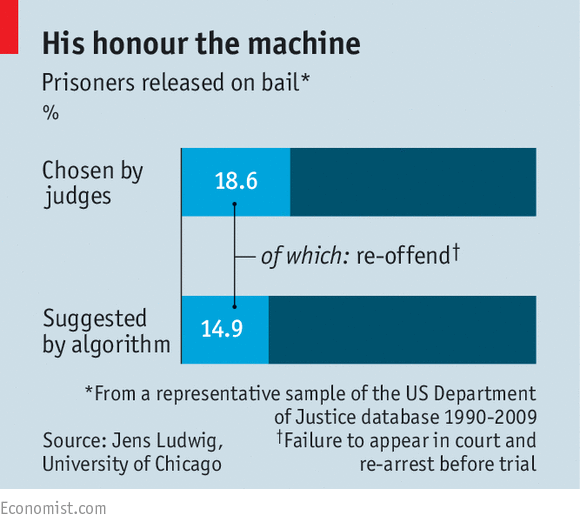
\includegraphics[width=\textwidth]{../figures/judge-fairness}
        }
      \end{column}
    \end{columns}
  }
  
  \only<article>{
    \begin{figure}
      \centering
      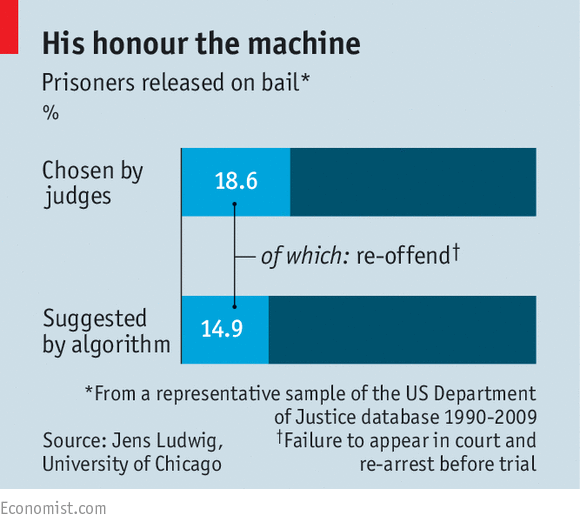
\includegraphics[width=0.5\textwidth]{../figures/judge-fairness}
      \caption{In some cases, it appears as though automating this procedure might lead to better outcomes. But is that generally true?}
      \label{fig:judge-fairness}
    \end{figure}
  }

\end{frame}

\begin{frame}
  \frametitle{Whites get lower scores than blacks\footnote{Pro-publica, 2016}}
  \only<article>{In a different study, it was shown that a commonly used software tool for determining 'risk scores' in the US was biased towards white defendants, who seemed to be always getting lower scores than blacks.}
  \begin{figure}[H]
    \begin{columns}
      \begin{column}{0.5\textwidth}
        \centering
        \def\svgwidth{0.45\textwidth}
        \input{../figures/risk-scores-black.pdf_tex}
        Black
      \end{column}
      \begin{column}{0.5\textwidth}
        \centering
        \def\svgwidth{0.45\textwidth}
        \input{../figures/risk-scores-white.pdf_tex}      
        White
      \end{column}
    \end{columns}
    \label{fig:risk-bias}
    \caption{Apparent bias in risk scores towards black versus white defendants.}
  \end{figure}
\end{frame}

\begin{frame}
  \frametitle{But scores equally accurately predict recidivsm\footnote{Washington Post, 2016}}
  \only<article>{On the other hand, the scores generated by the software seemed to be very predictive on whether or not defendants would re-offend, independently of their race.}
  \begin{figure}[H]
    \centering
    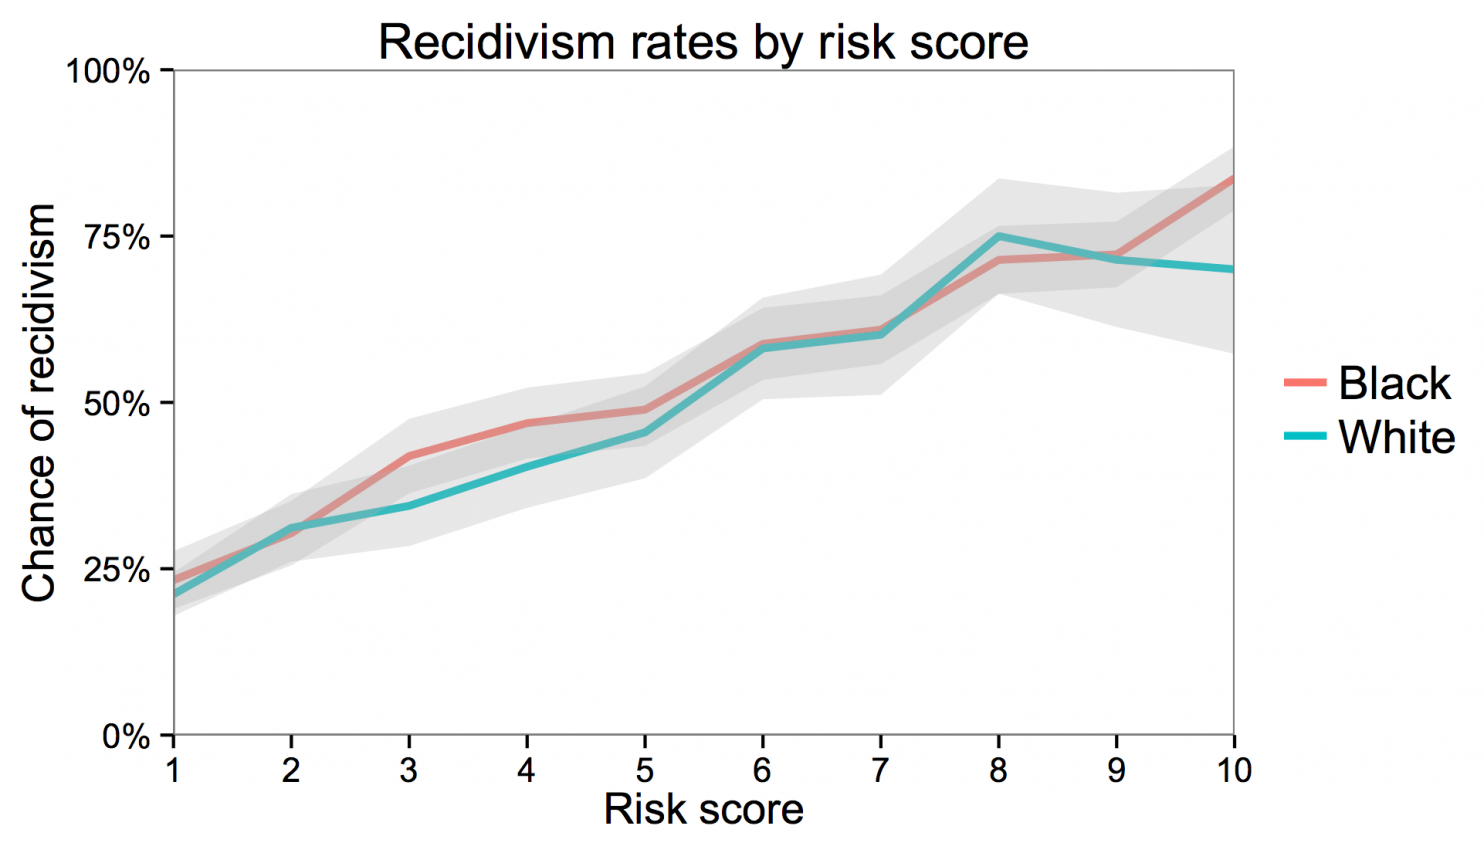
\includegraphics[width=\columnwidth]{../figures/imrs}
    \caption{Recidivism rates by risk score.}
    \label{fig:imrs}
  \end{figure}
\end{frame}
\begin{frame}
  \frametitle{But non-offending blacks get higher scores}
  \only<article>{On the third hand, we see that the system seemed to give higher risk scores to non-offending blacks. So, is there a way to fix that or not?}
  \begin{figure}[H]
    \centering
    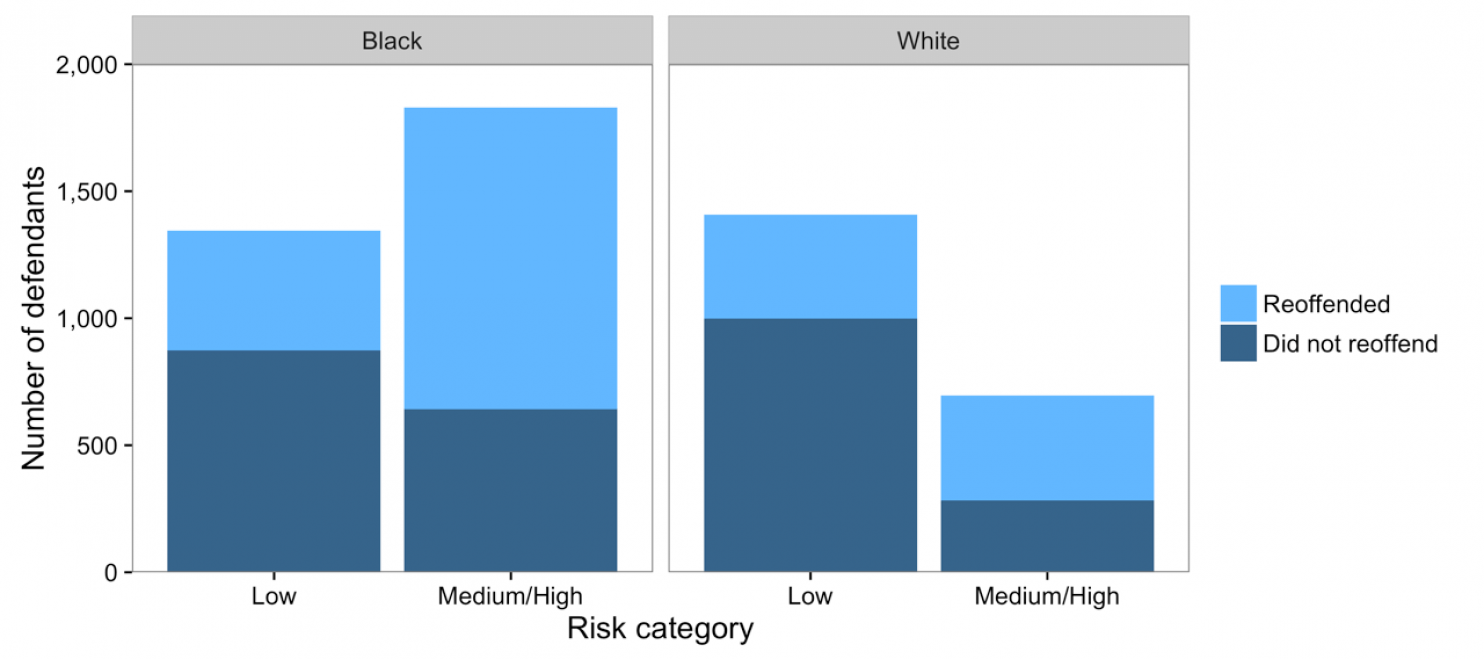
\includegraphics[width=0.5\textwidth]{../figures/imrs-risk}
    \caption{Score breakdown based on recidivism rates.}
    \label{fig:imrs-risk}
  \end{figure}
\end{frame}

\begin{frame}
  \frametitle{Bail decisions, revisited}
  \only<article>{Let us think of this problem in terms of bail decisions made by a judge using some policy $\pol$ with $\pol(a \mid x)$ being the probability that the judge decides $a$ when she observes $x$. Let $y$ be the outcome, which may or may not depend on $a$. In this particular case, $a$ is either release or jail. And $y$ is appears for trial or not. If we accept the tenets of decision theory, there is also a utility function $U(a, y)$ defined on which the judge bases her decision.}
  \only<presentation>{
    \centering

    \begin{columns}
      \begin{column}{0.5\textwidth}
        \begin{tikzpicture}
          \node[label=$x$] at (-1,2) (person)
          {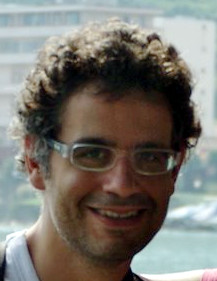
\includegraphics[width=0.2\columnwidth]{../figures/me-recent}};
          \node[label=$\pi$] at (0,0) (judge) {
\includegraphics[width=0.3\columnwidth]{../figures/judge}};
          \draw[->] (person) -- (judge);
          \uncover<2->{
            \node[label=$a_1$] at (-2,-2) (jail) {
\includegraphics[width=0.3\columnwidth]{../figures/jail}};
            \draw[->] (judge) -- (jail);
          }
          \uncover<3->{
            \node[label=$a_2$] at (2,-2) (bail) {
\includegraphics[width=0.3\columnwidth]{../figures/bail}};
            \draw[->] (judge) -- (bail);
          }
          \uncover<4->{
            \node[label=$y_1$] at (-2,-4) (trial) {
\includegraphics[width=0.3\columnwidth]{../figures/trial}};
            \draw[->] (jail) -- (trial);
          }
          \uncover<5->{
            \draw[->] (bail) -- (trial);
          }
          \uncover<6->{
            \node[label=$y_2$] at (2,-4) (arrest) {
\includegraphics[width=0.3\columnwidth]{../figures/handcuffs}};
            \draw[->] (bail) -- (arrest);
          }
        \end{tikzpicture}
      \end{column}
      \begin{column}{0.5\textwidth}
        \uncover<2->{\[\pi(a \mid x) \tag{policy}\]}
        \uncover<4->{\[\Pr(y \mid a, x) \tag{outcome}\]}
        \uncover<7->{\[U(a,y) \tag{utility}\]}
      \end{column}
    \end{columns}
  }
  \only<article>{
    \begin{figure}[H]
      \centering
      \begin{tikzpicture}
        \node[label=$x$] at (-1,3) (person)
        {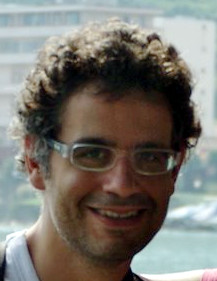
\includegraphics[width=0.1\textwidth]{../figures/me-recent}};
        \node[label=$\pi$] at (0,0) (judge) {
\includegraphics[width=0.2\textwidth]{../figures/judge}};
        \draw[->] (person) -- (judge);
        \uncover<2->{
          \node[label=$a_1$] at (-2,-3) (jail) {
\includegraphics[width=0.2\textwidth]{../figures/jail}};
          \draw[->] (judge) -- (jail);
        }
        \uncover<3->{
          \node[label=$a_2$] at (2,-3) (bail) {
\includegraphics[width=0.2\textwidth]{../figures/bail}};
          \draw[->] (judge) -- (bail);
        }
        \uncover<4->{
          \node[label=$y_1$] at (-2,-6) (trial) {
\includegraphics[width=0.2\textwidth]{../figures/trial}};
          \draw[->] (jail) -- (trial);
        }
        \uncover<5->{
          \draw[->] (bail) -- (trial);
        }
        \uncover<6->{
          \node[label=$y_2$] at (2,-6) (arrest) {
\includegraphics[width=0.2\textwidth]{../figures/handcuffs}};
          \draw[->] (bail) -- (arrest);
        }
      \end{tikzpicture}
      \caption{The bail decision process, simplified.}
      \label{fig:bail-process}
    \end{figure}
  }
\end{frame}


\subsection{Fairness as independence}
\begin{frame}
  \only<article>{So how can we reframe the above fairness notions in a more precise way? Both of them involve conditional independence between $y, a$ and a sensitive attribute $z$, such as race. The first notion says that the actions of the judge (or equivalently, the scores of the algorithm) are \emph{calibrated} with respect to the outcomes. The second says that they are \emph{balanced}, so that were the outcome known to the judge, she would be making a decision independently of the defendant's race.}
  \only<presentation>{
    \only<1>{
      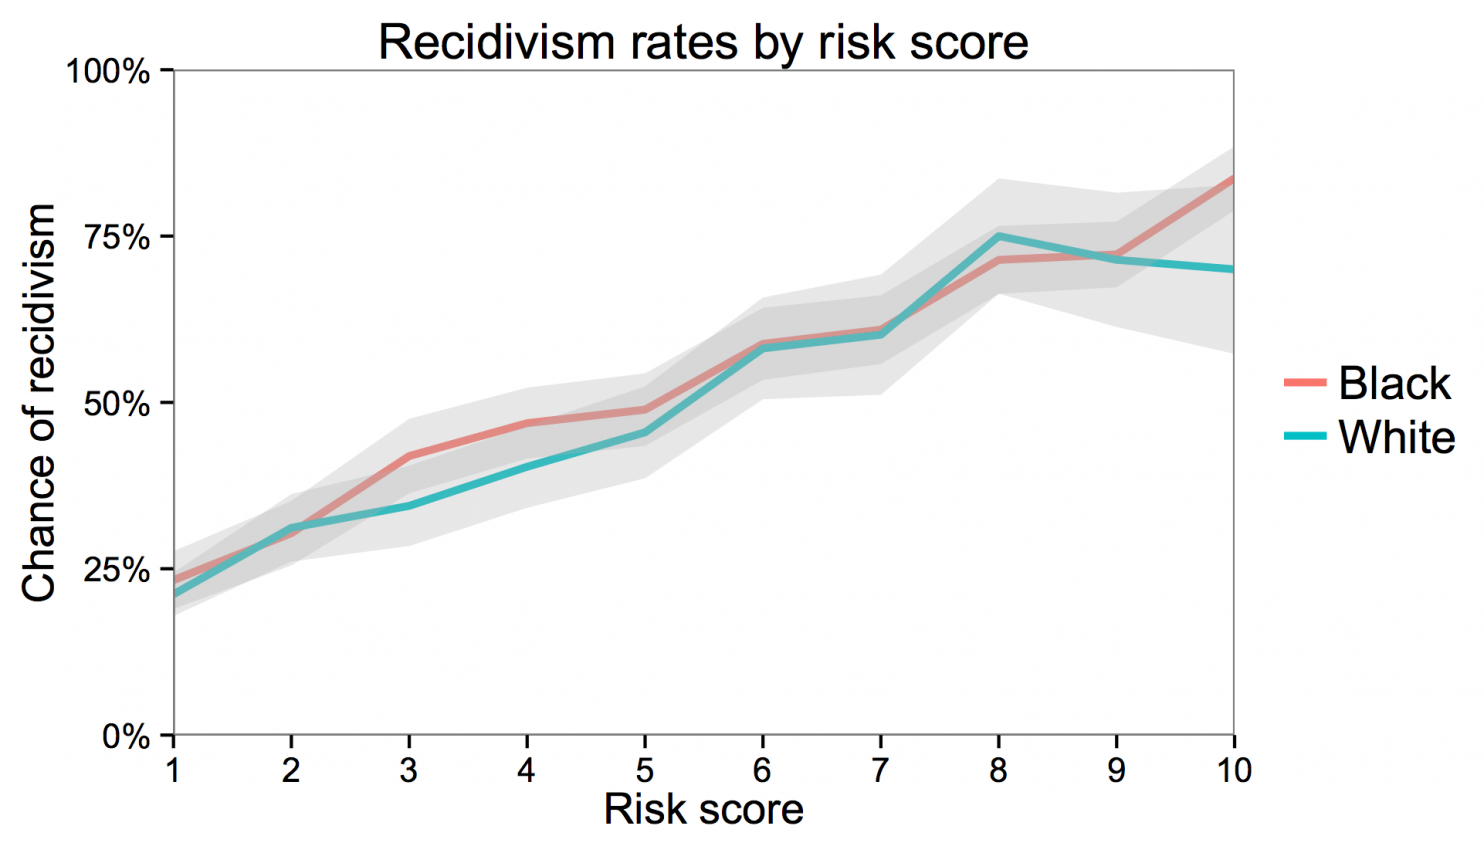
\includegraphics[width=\columnwidth]{../figures/imrs}
    }
    \only<2>{
      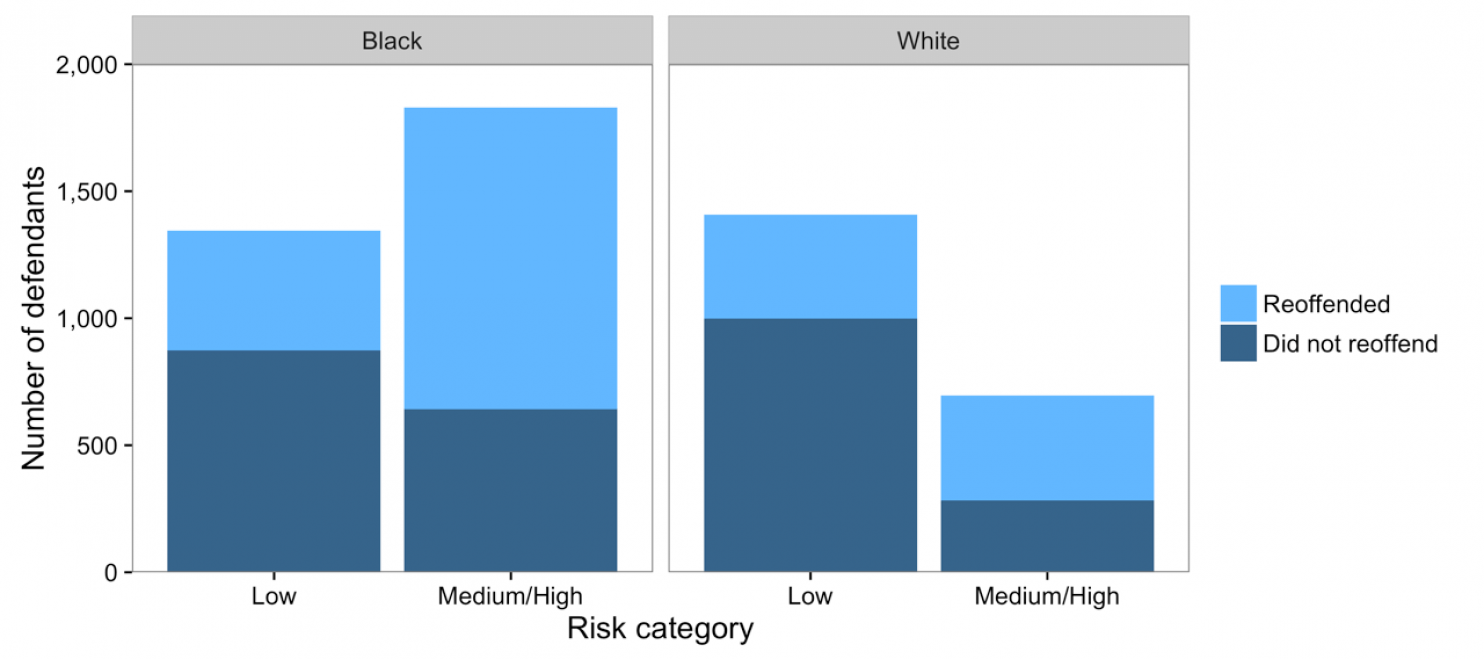
\includegraphics[width=\columnwidth]{../figures/imrs-risk}
    }
    \begin{columns}
      \begin{column}{0.3\textwidth}
        \begin{itemize}
        \item[$y$] Result.
        \item[$a$] Assigned score.
        \item[$z$] Race.
        \end{itemize}
      \end{column}
      \begin{column}{0.7\textwidth}
        \begin{align}
          \Pr^\pi(y \mid a, z) &= \Pr^\pi(y \mid a) \tag{\alert<1>{calibration}}\\
          \Pr^{\pi}(a \mid y, z) &= \Pr^{\pi}(a \mid y) \tag{\alert<2>{balance}}
        \end{align}
      \end{column}
    \end{columns}
  }
  \only<article>{
    \begin{definition}[Calibration]
      A policy $\pol$ is calibrated for parameter $\param$ with respect to $z$ if
      \begin{equation}
        \Pr_\param^\pol(y \mid a, z) = \Pr_\param^\pol(y \mid a), \qquad \forall a, z.
        \label{eq:calibration}
      \end{equation}
    \end{definition}
    You will observe that calibration here means that
    \[
      y \indep z \mid a, \param, \pol
    \]
    i.e. that $y$ is independent of $z$ given the judge's action $a$, so the distribution of outcomes is the same for every one of our actions no matter what the value of $z$ is.

    \begin{definition}[Balance]
      A policy $\pol$ is balanced for parameter $\param$ with respect to $z$ if
      \begin{equation}
        \Pr_\param^{\pol}(a \mid y, z) = \Pr_\param^{\pol}(a \mid y), \qquad \forall y, z.
        \label{eq:balance}
    \end{equation}
    \end{definition}
    On the other hand, balance means that
    \[
      a \indep z \mid y,
    \]
    i.e. that $a$ is independent of $z$ given the true outcome $y$.\footnote{This definition only really makes sense when $y$ does not depend on $a$ at all. When this is not the case, it's easy to construct a random variable $y'$ that does not depend on $a$ so that $y$ can be written as a function $y(y', a)$. Then we can achieve balance with respect to $y'$.}
  }

  \only<article>{In both cases, we defined conditional independence for a fixed probability distribution $P_\param(x,y,z)$ on the various variables.}
\end{frame}

\subsection{Fairness as meritocracy.}
  \only<article>{A different concept of fairness is meritocracy. For example, if one candidate for a job is better than another, shouldn't that candidate be always preferred? How can we formalise this?}


\begin{frame}

  \only<article>{Let us consider merit from the point of view of the decision maker, who can either hire $(a_t = 1)$ or not hire $(a_t = 0)$ the $t$-th applicant. If the applicant has characteristics $x_t$ and merit $y_t$, the DM's decision has utility $U(a_t, y_t)$. In order to model meritocracy, we assign an inherent \emph{quality} to $y$, expressed as an ordering, so that $U(1, y) \geq U(1, y')$ if $y \geq y'$. Assuming $P_\param(x_t, y_t)$ is known to the DM then clearly she should make the decision by solving the following maximisation problem:
  }
  \begin{align}
    a_t(\param, x_t) \in \argmax_a \E_\param(U \mid a, x_t)
    &=
      \int_\CY U(a_t, y) \E_\param(U \mid a_t, x_t) 
  \end{align}
  
  \only<article>{
    Here, the notion of meritocracy is defined through our utility function. The expectation here is essentially taken because we may not know for certain what the quality attribute of a given person might be.
  }
\end{frame}
\subsection{Fairness as similarity.}
\begin{frame}
  \only<article>{It makes sense to combine the idea of meritocracy with that of similarity. That is, similar people should be treated similarly. This means that we should find a policy $\pol$ that maximises utility $\util$ and makes similar decisions for similar people. We can formalize this as}
  \[
  D(\pol(a \mid x), \pol(a \mid x')
  \leq 
  \rho(x, x').
  \]
  \begin{tikzpicture}[scale=2,thick,domain=-2:2]
    \draw[->] (-2,0) -- (2,0) node[right] {$x$};
    \draw[->] (0,0) -- (0,1) node[above] {$\pol(a \mid x)$};
    \draw[color=blue] plot (\x,{0.5 + 0.5 * tanh(\x)}); % node[right] {$f(x) = \frac{1}{20} \mathrm e^x$};
    \draw [|<->|,color=red] plot (-0.5,-0.1) -- node[below=1em] {$\rho(x,x')$} ++(1, 0);
  \end{tikzpicture}
\end{frame}








%%% Local Variables:
%%% mode: latex
%%% TeX-engine: xetex
%%% TeX-master: "notes"
%%% End:


\chapter{Structured problems}

\chapter{Experiment design}

\end{document}
%%% Local Variables:
%%% mode: latex
%%% TeX-master: "notes"
%%% End:
